% Options for packages loaded elsewhere
% Options for packages loaded elsewhere
\PassOptionsToPackage{unicode}{hyperref}
\PassOptionsToPackage{hyphens}{url}
\PassOptionsToPackage{dvipsnames,svgnames,x11names}{xcolor}
%
\documentclass[
  12pt,
  letterpaper,
  DIV=11,
  numbers=noendperiod,
  oneside,
  open=any]{scrreprt}
\usepackage{xcolor}
\usepackage[top=30mm,bottom=30mm,left=25mm,right=25mm]{geometry}
\usepackage{amsmath,amssymb}
\setcounter{secnumdepth}{5}
\usepackage{iftex}
\ifPDFTeX
  \usepackage[T1]{fontenc}
  \usepackage[utf8]{inputenc}
  \usepackage{textcomp} % provide euro and other symbols
\else % if luatex or xetex
  \usepackage{unicode-math} % this also loads fontspec
  \defaultfontfeatures{Scale=MatchLowercase}
  \defaultfontfeatures[\rmfamily]{Ligatures=TeX,Scale=1}
\fi
\usepackage{lmodern}
\ifPDFTeX\else
  % xetex/luatex font selection
  \setmainfont[]{Times New Roman}
  \setsansfont[]{Arial}
  \setmonofont[]{Courier New}
\fi
% Use upquote if available, for straight quotes in verbatim environments
\IfFileExists{upquote.sty}{\usepackage{upquote}}{}
\IfFileExists{microtype.sty}{% use microtype if available
  \usepackage[]{microtype}
  \UseMicrotypeSet[protrusion]{basicmath} % disable protrusion for tt fonts
}{}
\usepackage{setspace}
\makeatletter
\@ifundefined{KOMAClassName}{% if non-KOMA class
  \IfFileExists{parskip.sty}{%
    \usepackage{parskip}
  }{% else
    \setlength{\parindent}{0pt}
    \setlength{\parskip}{6pt plus 2pt minus 1pt}}
}{% if KOMA class
  \KOMAoptions{parskip=half}}
\makeatother
% Make \paragraph and \subparagraph free-standing
\makeatletter
\ifx\paragraph\undefined\else
  \let\oldparagraph\paragraph
  \renewcommand{\paragraph}{
    \@ifstar
      \xxxParagraphStar
      \xxxParagraphNoStar
  }
  \newcommand{\xxxParagraphStar}[1]{\oldparagraph*{#1}\mbox{}}
  \newcommand{\xxxParagraphNoStar}[1]{\oldparagraph{#1}\mbox{}}
\fi
\ifx\subparagraph\undefined\else
  \let\oldsubparagraph\subparagraph
  \renewcommand{\subparagraph}{
    \@ifstar
      \xxxSubParagraphStar
      \xxxSubParagraphNoStar
  }
  \newcommand{\xxxSubParagraphStar}[1]{\oldsubparagraph*{#1}\mbox{}}
  \newcommand{\xxxSubParagraphNoStar}[1]{\oldsubparagraph{#1}\mbox{}}
\fi
\makeatother

\usepackage{color}
\usepackage{fancyvrb}
\newcommand{\VerbBar}{|}
\newcommand{\VERB}{\Verb[commandchars=\\\{\}]}
\DefineVerbatimEnvironment{Highlighting}{Verbatim}{commandchars=\\\{\}}
% Add ',fontsize=\small' for more characters per line
\usepackage{framed}
\definecolor{shadecolor}{RGB}{248,248,248}
\newenvironment{Shaded}{\begin{snugshade}}{\end{snugshade}}
\newcommand{\AlertTok}[1]{\textcolor[rgb]{0.94,0.16,0.16}{#1}}
\newcommand{\AnnotationTok}[1]{\textcolor[rgb]{0.56,0.35,0.01}{\textbf{\textit{#1}}}}
\newcommand{\AttributeTok}[1]{\textcolor[rgb]{0.13,0.29,0.53}{#1}}
\newcommand{\BaseNTok}[1]{\textcolor[rgb]{0.00,0.00,0.81}{#1}}
\newcommand{\BuiltInTok}[1]{#1}
\newcommand{\CharTok}[1]{\textcolor[rgb]{0.31,0.60,0.02}{#1}}
\newcommand{\CommentTok}[1]{\textcolor[rgb]{0.56,0.35,0.01}{\textit{#1}}}
\newcommand{\CommentVarTok}[1]{\textcolor[rgb]{0.56,0.35,0.01}{\textbf{\textit{#1}}}}
\newcommand{\ConstantTok}[1]{\textcolor[rgb]{0.56,0.35,0.01}{#1}}
\newcommand{\ControlFlowTok}[1]{\textcolor[rgb]{0.13,0.29,0.53}{\textbf{#1}}}
\newcommand{\DataTypeTok}[1]{\textcolor[rgb]{0.13,0.29,0.53}{#1}}
\newcommand{\DecValTok}[1]{\textcolor[rgb]{0.00,0.00,0.81}{#1}}
\newcommand{\DocumentationTok}[1]{\textcolor[rgb]{0.56,0.35,0.01}{\textbf{\textit{#1}}}}
\newcommand{\ErrorTok}[1]{\textcolor[rgb]{0.64,0.00,0.00}{\textbf{#1}}}
\newcommand{\ExtensionTok}[1]{#1}
\newcommand{\FloatTok}[1]{\textcolor[rgb]{0.00,0.00,0.81}{#1}}
\newcommand{\FunctionTok}[1]{\textcolor[rgb]{0.13,0.29,0.53}{\textbf{#1}}}
\newcommand{\ImportTok}[1]{#1}
\newcommand{\InformationTok}[1]{\textcolor[rgb]{0.56,0.35,0.01}{\textbf{\textit{#1}}}}
\newcommand{\KeywordTok}[1]{\textcolor[rgb]{0.13,0.29,0.53}{\textbf{#1}}}
\newcommand{\NormalTok}[1]{#1}
\newcommand{\OperatorTok}[1]{\textcolor[rgb]{0.81,0.36,0.00}{\textbf{#1}}}
\newcommand{\OtherTok}[1]{\textcolor[rgb]{0.56,0.35,0.01}{#1}}
\newcommand{\PreprocessorTok}[1]{\textcolor[rgb]{0.56,0.35,0.01}{\textit{#1}}}
\newcommand{\RegionMarkerTok}[1]{#1}
\newcommand{\SpecialCharTok}[1]{\textcolor[rgb]{0.81,0.36,0.00}{\textbf{#1}}}
\newcommand{\SpecialStringTok}[1]{\textcolor[rgb]{0.31,0.60,0.02}{#1}}
\newcommand{\StringTok}[1]{\textcolor[rgb]{0.31,0.60,0.02}{#1}}
\newcommand{\VariableTok}[1]{\textcolor[rgb]{0.00,0.00,0.00}{#1}}
\newcommand{\VerbatimStringTok}[1]{\textcolor[rgb]{0.31,0.60,0.02}{#1}}
\newcommand{\WarningTok}[1]{\textcolor[rgb]{0.56,0.35,0.01}{\textbf{\textit{#1}}}}

\usepackage{longtable,booktabs,array}
\usepackage{calc} % for calculating minipage widths
% Correct order of tables after \paragraph or \subparagraph
\usepackage{etoolbox}
\makeatletter
\patchcmd\longtable{\par}{\if@noskipsec\mbox{}\fi\par}{}{}
\makeatother
% Allow footnotes in longtable head/foot
\IfFileExists{footnotehyper.sty}{\usepackage{footnotehyper}}{\usepackage{footnote}}
\makesavenoteenv{longtable}
\usepackage{graphicx}
\makeatletter
\newsavebox\pandoc@box
\newcommand*\pandocbounded[1]{% scales image to fit in text height/width
  \sbox\pandoc@box{#1}%
  \Gscale@div\@tempa{\textheight}{\dimexpr\ht\pandoc@box+\dp\pandoc@box\relax}%
  \Gscale@div\@tempb{\linewidth}{\wd\pandoc@box}%
  \ifdim\@tempb\p@<\@tempa\p@\let\@tempa\@tempb\fi% select the smaller of both
  \ifdim\@tempa\p@<\p@\scalebox{\@tempa}{\usebox\pandoc@box}%
  \else\usebox{\pandoc@box}%
  \fi%
}
% Set default figure placement to htbp
\def\fps@figure{htbp}
\makeatother


% definitions for citeproc citations
\NewDocumentCommand\citeproctext{}{}
\NewDocumentCommand\citeproc{mm}{%
  \begingroup\def\citeproctext{#2}\cite{#1}\endgroup}
\makeatletter
 % allow citations to break across lines
 \let\@cite@ofmt\@firstofone
 % avoid brackets around text for \cite:
 \def\@biblabel#1{}
 \def\@cite#1#2{{#1\if@tempswa , #2\fi}}
\makeatother
\newlength{\cslhangindent}
\setlength{\cslhangindent}{1.5em}
\newlength{\csllabelwidth}
\setlength{\csllabelwidth}{3em}
\newenvironment{CSLReferences}[2] % #1 hanging-indent, #2 entry-spacing
 {\begin{list}{}{%
  \setlength{\itemindent}{0pt}
  \setlength{\leftmargin}{0pt}
  \setlength{\parsep}{0pt}
  % turn on hanging indent if param 1 is 1
  \ifodd #1
   \setlength{\leftmargin}{\cslhangindent}
   \setlength{\itemindent}{-1\cslhangindent}
  \fi
  % set entry spacing
  \setlength{\itemsep}{#2\baselineskip}}}
 {\end{list}}
\usepackage{calc}
\newcommand{\CSLBlock}[1]{\hfill\break\parbox[t]{\linewidth}{\strut\ignorespaces#1\strut}}
\newcommand{\CSLLeftMargin}[1]{\parbox[t]{\csllabelwidth}{\strut#1\strut}}
\newcommand{\CSLRightInline}[1]{\parbox[t]{\linewidth - \csllabelwidth}{\strut#1\strut}}
\newcommand{\CSLIndent}[1]{\hspace{\cslhangindent}#1}



\setlength{\emergencystretch}{3em} % prevent overfull lines

\providecommand{\tightlist}{%
  \setlength{\itemsep}{0pt}\setlength{\parskip}{0pt}}



 


\usepackage{booktabs}
\usepackage{caption}
\usepackage{longtable}
\usepackage{colortbl}
\usepackage{array}
\usepackage{anyfontsize}
\usepackage{multirow}
\KOMAoption{captions}{tableheading}
\makeatletter
\@ifpackageloaded{tcolorbox}{}{\usepackage[skins,breakable]{tcolorbox}}
\@ifpackageloaded{fontawesome5}{}{\usepackage{fontawesome5}}
\definecolor{quarto-callout-color}{HTML}{909090}
\definecolor{quarto-callout-note-color}{HTML}{0758E5}
\definecolor{quarto-callout-important-color}{HTML}{CC1914}
\definecolor{quarto-callout-warning-color}{HTML}{EB9113}
\definecolor{quarto-callout-tip-color}{HTML}{00A047}
\definecolor{quarto-callout-caution-color}{HTML}{FC5300}
\definecolor{quarto-callout-color-frame}{HTML}{acacac}
\definecolor{quarto-callout-note-color-frame}{HTML}{4582ec}
\definecolor{quarto-callout-important-color-frame}{HTML}{d9534f}
\definecolor{quarto-callout-warning-color-frame}{HTML}{f0ad4e}
\definecolor{quarto-callout-tip-color-frame}{HTML}{02b875}
\definecolor{quarto-callout-caution-color-frame}{HTML}{fd7e14}
\makeatother
\makeatletter
\@ifpackageloaded{bookmark}{}{\usepackage{bookmark}}
\makeatother
\makeatletter
\@ifpackageloaded{caption}{}{\usepackage{caption}}
\AtBeginDocument{%
\ifdefined\contentsname
  \renewcommand*\contentsname{Table of contents}
\else
  \newcommand\contentsname{Table of contents}
\fi
\ifdefined\listfigurename
  \renewcommand*\listfigurename{List of Figures}
\else
  \newcommand\listfigurename{List of Figures}
\fi
\ifdefined\listtablename
  \renewcommand*\listtablename{List of Tables}
\else
  \newcommand\listtablename{List of Tables}
\fi
\ifdefined\figurename
  \renewcommand*\figurename{Figure}
\else
  \newcommand\figurename{Figure}
\fi
\ifdefined\tablename
  \renewcommand*\tablename{Table}
\else
  \newcommand\tablename{Table}
\fi
}
\@ifpackageloaded{float}{}{\usepackage{float}}
\floatstyle{ruled}
\@ifundefined{c@chapter}{\newfloat{codelisting}{h}{lop}}{\newfloat{codelisting}{h}{lop}[chapter]}
\floatname{codelisting}{Listing}
\newcommand*\listoflistings{\listof{codelisting}{List of Listings}}
\makeatother
\makeatletter
\makeatother
\makeatletter
\@ifpackageloaded{caption}{}{\usepackage{caption}}
\@ifpackageloaded{subcaption}{}{\usepackage{subcaption}}
\makeatother
\makeatletter
\@ifpackageloaded{tcolorbox}{}{\usepackage[skins,breakable]{tcolorbox}}
\makeatother
\makeatletter
\@ifundefined{shadecolor}{\definecolor{shadecolor}{HTML}{E83E8C}}{}
\makeatother
\makeatletter
\makeatother
\makeatletter
\ifdefined\Shaded\renewenvironment{Shaded}{\begin{tcolorbox}[interior hidden, frame hidden, breakable, borderline west={3pt}{0pt}{shadecolor}, enhanced, sharp corners, boxrule=0pt]}{\end{tcolorbox}}\fi
\makeatother
\makeatletter
\@ifpackageloaded{sidenotes}{}{\usepackage{sidenotes}}
\@ifpackageloaded{marginnote}{}{\usepackage{marginnote}}
\makeatother
\usepackage{bookmark}
\IfFileExists{xurl.sty}{\usepackage{xurl}}{} % add URL line breaks if available
\urlstyle{same}
\hypersetup{
  pdftitle={Biostatistics with R},
  pdfauthor={Bikram Adhikari},
  colorlinks=true,
  linkcolor={NavyBlue},
  filecolor={Maroon},
  citecolor={NavyBlue},
  urlcolor={NavyBlue},
  pdfcreator={LaTeX via pandoc}}


\title{Biostatistics with R}
\usepackage{etoolbox}
\makeatletter
\providecommand{\subtitle}[1]{% add subtitle to \maketitle
  \apptocmd{\@title}{\par {\large #1 \par}}{}{}
}
\makeatother
\subtitle{A Practical Guide for Public Health Researchers}
\author{Bikram Adhikari}
\date{August 8, 2026}
\begin{document}
\maketitle

\renewcommand*\contentsname{Table of contents}
{
\hypersetup{linkcolor=}
\setcounter{tocdepth}{2}
\tableofcontents
}
\listoffigures
\listoftables

\setstretch{1.5}
\bookmarksetup{startatroot}

\chapter*{Preface}\label{preface}
\addcontentsline{toc}{chapter}{Preface}

\markboth{Preface}{Preface}

I'm writing this note book as a student, and I wrote it for students.

When I first started working with epidemiology and biostatistics, I
found plenty of resources explaining concepts, but very few showing how
to actually apply them using real data. I often struggled with cleaning
datasets, choosing the right methods, or understanding why my results
didn't make sense. Most explanations were either too technical or too
vague. I kept wishing for a practical, clear guide written from a
learner's perspective.

This book is my attempt to do exactly that.

It begins with the basics such as data import, cleaning, and descriptive
analysis, and gradually builds toward regression models, study design,
and interpretation. The focus is on practical application using R, with
clear explanations before code and simple interpretations after.

This is not a theoretical textbook. It is a hands-on guide to real
problems researchers face.

I hope it helps you learn, apply, and grow with confidence.

\part{Introduction to R}

\chapter{Introduction to R}\label{introduction-to-r-1}

\section{Background}\label{background}

R originated in the early 1990s as a free and open-source alternative to
the commercial statistical programming language S-PLUS. It was created
by \textbf{Ross Ihaka} and \textbf{Robert Gentleman} at the University
of Auckland, New Zealand. After two years in 1993 the R was made public
and its development continued with contributions from various
researchers and statisticians globally. In 1995, Martin Mächler played a
significant role in convincing Ross Ihaka and Robert Gentalman to adopt
GNU General Public License, making R free software(Ihaka, n.d.a) . Over
the years, R has evolved into a powerful tool for statistical computing,
data analysis, and visualization, with thousands of packages available
for various tasks. Its active development, frequent releases, and robust
graphics capabilities have contributed to its widespread adoption across
industry, academia, and research. Today, R is considered as one of the
most popular languages in data science and statistical analysis({``R for
Data Analysis - 1 What Is R?''} n.d.; Ihaka, n.d.b).

\section{Why to learn R?}\label{why-to-learn-r}

\begin{enumerate}
\def\labelenumi{\arabic{enumi}.}
\tightlist
\item
  R is free and open source tool.
\item
  It has large community of users.
\item
  It is a independent platform.
\item
  It has a robust visualization library.
\item
  It is use in almost every industry including health, finance.
\item
  It is hottest in trend.
\item
  Large number of packages are available which enables users with the
  extensive toolkit for data manipulation, analysis and machine
  learning.
\end{enumerate}

\section{Setup R in your computer}\label{setup-r-in-your-computer}

R requires installation of console R and R-studio in your computer.
Follow the instruction below to setup R in your computer

\subsection{Download and install R}\label{download-and-install-r}

\begin{enumerate}
\def\labelenumi{\arabic{enumi}.}
\item
  Open an internet browser and go to
  \url{https://cran.r-project.org/bin/} ({``The Comprehensive r Archive
  Network,''} n.d.).
\item
  Click the required Operating system. For Windows find the link
  ``\href{https://cran.r-project.org/bin/windows/base/}{install R for
  the first time}'' and for MacOSX click the link
  ``\href{https://cran.r-project.org/bin/macosx/}{macosx/}''
\item
  For windows click on link ``Download R for Windows''. For macOS find
  link with the name ``R-x.x.x-arm64.pkg'' or ``R-x.x.x-x86\_64.pkg''.
  Click one of them based on your macOS type
\item
  Download R executable file and save them somewhere on your computer.
  Run the executable file and follow the installation instructions.
\end{enumerate}

\subsection{Download and install
RStudio.}\label{download-and-install-rstudio.}

\begin{enumerate}
\def\labelenumi{\arabic{enumi}.}
\item
  To Install R-studio go to
  \url{https://posit.co/download/rstudio-desktop/} ({``RStudio IDE User
  Guide''} 2026).
\item
  Click on ``Download RStudio Desktop'', and save the executable file
  somewhere on your computer. Run the executable file and follow the
  installation instructions.
\end{enumerate}

\section{RStudio Interface}\label{rstudio-interface}

R Studio is an integrated development environment (IDE) for R. It has
four main panes, top-left, top-right, bottom-left and bottom-right. Each
panes has specific purpose.

\begin{figure}[H]

{\centering \pandocbounded{
\includegraphics[keepaspectratio]{section1/Chapter1/Pictures/picture_2.png}}

}

\caption{\emph{Figure 1: RStudio interface showing four panes}}

\end{figure}%

\textbf{Top-Left (Text editor, R-script, R-markdown, Quarto)}

This is where you can write and edit script that you want to run. You
can type multiple lines of code into the text editor without having each
line evaluated by R. You can save and share the code! There are a few
other ways to write R scripts, that may be useful in the future. (such
as R-markdown, R notebooks, quarto book or making slides.)

\textbf{Top-Right (Environment, History, Tutorials)}

\emph{Environment:} The Environment tab stores and shows all of the
active objects, values, and functions (and anything else you create)
during your R session. R stores both data and output from data analysis
(as well as everything else) in objects. Once you create an object, it
should appear in the RStudio Environment pane.

\emph{History:} You can explore your history if you've lost a command or
variable that you want back. It's searchable to make finding that
missing command super easy!

\emph{Tutorials:} You can get tutorials on R in this section.

\textbf{Bottom-left (R Console)}

The R console is the pane where R is waiting for us to tell it what to
do, and where it will show the results of the commands. We can type
directly into console, but they will be forgotten once we close the
session.

\textbf{Bottom Right}

\emph{Plots:} Any plots that you produce be in the ``Plots'' tab. It
will keep a history so you can see changes as you make them.

\emph{Packages:} You can download new packages by clicking Packages
-\textgreater{} Install. You can load packages by checking them off, but
this is best done in your scripts!

\emph{Help:} Have a question on syntax of a command? You can look at
it's help page by searching for it. You can also poke around tutorials
and FAQ.

\emph{Working Directory:} Files in the working directory, you can change
your working directory to anything else in the code or by going to that
location and clicking \emph{More -\textgreater{} Set as Directory}.

\section{Important shortcuts}\label{important-shortcuts}

You can get list of important shortcuts by navigating \emph{Tools
\textgreater{} Keyboard Shortcuts Help} or \texttt{ALT+SHIFT+K} Shortcut
keys can help to efficient coding.

\pandocbounded{
\includegraphics[keepaspectratio]{section1/Chapter1/Pictures/picture_6.png}}
\# RStudio Keyboard Shortcuts (Windows/Linux)

\subsection{File Management}\label{file-management}

\begin{longtable}[]{@{}ll@{}}
\toprule\noalign{}
Shortcut & Action \\
\midrule\noalign{}
\endhead
\bottomrule\noalign{}
\endlastfoot
\texttt{Ctrl+N} & New Script \\
\texttt{Ctrl+Shift+N} & New R Script \\
\texttt{Ctrl+O} & Open File \\
\texttt{Ctrl+S} & Save \\
\texttt{Ctrl+Alt+S} & Save All \\
\texttt{Ctrl+Shift+W} & Close All \\
\texttt{Ctrl+W} & Close Current File \\
\texttt{Ctrl+Shift+F4} & Close All Except Current \\
\texttt{Ctrl+P} & Open File Quickly \\
\end{longtable}

\begin{center}\rule{0.5\linewidth}{0.5pt}\end{center}

\subsection{Running Code}\label{running-code}

\begin{longtable}[]{@{}ll@{}}
\toprule\noalign{}
Shortcut & Action \\
\midrule\noalign{}
\endhead
\bottomrule\noalign{}
\endlastfoot
\texttt{Ctrl+Enter} & Run Current Line/Selection \\
\texttt{Alt+Enter} & Run Without Moving Cursor \\
\texttt{Ctrl+Alt+R} & Run All \\
\texttt{Ctrl+Alt+B} & Run from Beginning to Cursor \\
\texttt{Ctrl+Alt+E} & Run from Cursor to End \\
\texttt{Ctrl+Alt+F} & Run Current Function \\
\texttt{Ctrl+Alt+T} & Run Current Section \\
\texttt{Ctrl+Shift+Enter} & Source Current Script \\
\texttt{Ctrl+Shift+S} & Source Active File \\
\texttt{Ctrl+Alt+Enter} & Send to Terminal \\
\end{longtable}

\begin{center}\rule{0.5\linewidth}{0.5pt}\end{center}

\subsection{R Markdown / Quarto}\label{r-markdown-quarto}

\begin{longtable}[]{@{}ll@{}}
\toprule\noalign{}
Shortcut & Action \\
\midrule\noalign{}
\endhead
\bottomrule\noalign{}
\endlastfoot
\texttt{Ctrl+Alt+I} & Insert Code Chunk \\
\texttt{Ctrl+Shift+K} & Render / Knit Document \\
\texttt{Ctrl+Shift+F10} & Restart R Session \\
\texttt{Ctrl+Shift+C} & Comment / Uncomment Lines \\
\end{longtable}

\begin{center}\rule{0.5\linewidth}{0.5pt}\end{center}

\subsection{Code Editing}\label{code-editing}

\begin{longtable}[]{@{}ll@{}}
\toprule\noalign{}
Shortcut & Action \\
\midrule\noalign{}
\endhead
\bottomrule\noalign{}
\endlastfoot
\texttt{Tab} & Autocomplete \\
\texttt{Ctrl+Space} & Code Completion \\
\texttt{Ctrl+Shift+A} & Reformat Code \\
\texttt{Ctrl+D} & Delete Line \\
\texttt{Ctrl+Z} & Undo \\
\texttt{Ctrl+Shift+Z} & Redo \\
\texttt{Ctrl+C} & Copy \\
\texttt{Ctrl+X} & Cut \\
\texttt{Ctrl+V} & Paste \\
\texttt{Ctrl+A} & Select All \\
\texttt{Ctrl+Y} & Insert Previously Yanked Text \\
\texttt{Ctrl+K} & Yank Line After Cursor \\
\texttt{Ctrl+U} & Delete Line \\
\texttt{Ctrl+Shift+M} & Insert Pipe \texttt{\%\textgreater{}\%} \\
\texttt{Ctrl+Alt+Shift+M} & Insert Native Pipe
\texttt{\textbar{}\textgreater{}} \\
\texttt{Ctrl+Alt+-} & Assignment Operator \texttt{\textless{}-} \\
\end{longtable}

\begin{center}\rule{0.5\linewidth}{0.5pt}\end{center}

\subsection{Multi-Cursor Editing}\label{multi-cursor-editing}

\begin{longtable}[]{@{}ll@{}}
\toprule\noalign{}
Shortcut & Action \\
\midrule\noalign{}
\endhead
\bottomrule\noalign{}
\endlastfoot
\texttt{Ctrl+Alt+Up} & Add Cursor Above \\
\texttt{Ctrl+Alt+Down} & Add Cursor Below \\
\texttt{Ctrl+Alt+Shift+Up} & Expand Selection \\
\texttt{Ctrl+Alt+Shift+Down} & Shrink Selection \\
\end{longtable}

\begin{center}\rule{0.5\linewidth}{0.5pt}\end{center}

\subsection{Navigation}\label{navigation}

\begin{longtable}[]{@{}ll@{}}
\toprule\noalign{}
Shortcut & Action \\
\midrule\noalign{}
\endhead
\bottomrule\noalign{}
\endlastfoot
\texttt{Ctrl+F} & Find \\
\texttt{Ctrl+H} & Replace \\
\texttt{Ctrl+Shift+F} & Find in Files \\
\texttt{Ctrl+F3} & Find Next \\
\texttt{Shift+F3} & Find Previous \\
\texttt{Ctrl+L} & Jump to Line \\
\texttt{Ctrl+Alt+G} & Go to Line \\
\texttt{Ctrl+.} & Go to File / Function \\
\texttt{Ctrl+1} & Move Focus to Source \\
\texttt{Ctrl+2} & Move Focus to Console \\
\texttt{Ctrl+Shift+.} & Switch to Last Tab \\
\texttt{Ctrl+Tab} & Next Tab \\
\texttt{Ctrl+Shift+Tab} & Previous Tab \\
\end{longtable}

\begin{center}\rule{0.5\linewidth}{0.5pt}\end{center}

\subsection{Folding Code}\label{folding-code}

\begin{longtable}[]{@{}ll@{}}
\toprule\noalign{}
Shortcut & Action \\
\midrule\noalign{}
\endhead
\bottomrule\noalign{}
\endlastfoot
\texttt{Alt+L} & Collapse Fold \\
\texttt{Alt+Shift+L} & Expand Fold \\
\texttt{Alt+O} & Collapse All Folds \\
\texttt{Alt+Shift+O} & Expand All Folds \\
\end{longtable}

\begin{center}\rule{0.5\linewidth}{0.5pt}\end{center}

\subsection{Console}\label{console}

\begin{longtable}[]{@{}ll@{}}
\toprule\noalign{}
Shortcut & Action \\
\midrule\noalign{}
\endhead
\bottomrule\noalign{}
\endlastfoot
\texttt{Ctrl+Up} & Command History \\
\texttt{Esc} & Interrupt Running Code \\
\texttt{Ctrl+L} & Clear Console \\
\texttt{Ctrl+Shift+F10} & Restart R \\
\end{longtable}

\begin{center}\rule{0.5\linewidth}{0.5pt}\end{center}

\subsection{Debugging}\label{debugging}

\begin{longtable}[]{@{}ll@{}}
\toprule\noalign{}
Shortcut & Action \\
\midrule\noalign{}
\endhead
\bottomrule\noalign{}
\endlastfoot
\texttt{Shift+F9} & Toggle Breakpoint \\
\texttt{F10} & Step Over \\
\texttt{Shift+F4} & Step Into \\
\texttt{Shift+F7} & Finish Function \\
\texttt{Shift+F5} & Continue \\
\texttt{Shift+F8} & Stop Debugging \\
\end{longtable}

\begin{center}\rule{0.5\linewidth}{0.5pt}\end{center}

\subsection{Pane Navigation}\label{pane-navigation}

\begin{longtable}[]{@{}ll@{}}
\toprule\noalign{}
Shortcut & Action \\
\midrule\noalign{}
\endhead
\bottomrule\noalign{}
\endlastfoot
\texttt{Ctrl+1} & Source \\
\texttt{Ctrl+2} & Console \\
\texttt{Ctrl+3} & Help \\
\texttt{Ctrl+4} & History \\
\texttt{Ctrl+5} & Files \\
\texttt{Ctrl+6} & Plots \\
\texttt{Ctrl+7} & Packages \\
\texttt{Ctrl+8} & Environment \\
\texttt{Ctrl+9} & Viewer \\
\texttt{F6} & Next Pane \\
\texttt{Shift+F6} & Previous Pane \\
\end{longtable}

\begin{center}\rule{0.5\linewidth}{0.5pt}\end{center}

\subsection{Tabs}\label{tabs}

\begin{longtable}[]{@{}ll@{}}
\toprule\noalign{}
Shortcut & Action \\
\midrule\noalign{}
\endhead
\bottomrule\noalign{}
\endlastfoot
\texttt{Ctrl+Shift+.} & Switch to Last Tab \\
\texttt{Ctrl+Tab} & Next Tab \\
\texttt{Ctrl+Shift+Tab} & Previous Tab \\
\texttt{Ctrl+Shift+F11} & First Tab \\
\texttt{Ctrl+Shift+F12} & Last Tab \\
\end{longtable}

\begin{center}\rule{0.5\linewidth}{0.5pt}\end{center}

\subsection{Terminal}\label{terminal}

\begin{longtable}[]{@{}ll@{}}
\toprule\noalign{}
Shortcut & Action \\
\midrule\noalign{}
\endhead
\bottomrule\noalign{}
\endlastfoot
\texttt{Alt+Shift+R} & New Terminal \\
\texttt{Alt+Shift+M} & Focus Terminal \\
\texttt{Alt+Shift+F11} & Previous Terminal \\
\texttt{Alt+Shift+F12} & Next Terminal \\
\end{longtable}

\begin{center}\rule{0.5\linewidth}{0.5pt}\end{center}

\subsection{Build}\label{build}

\begin{longtable}[]{@{}ll@{}}
\toprule\noalign{}
Shortcut & Action \\
\midrule\noalign{}
\endhead
\bottomrule\noalign{}
\endlastfoot
\texttt{Ctrl+Shift+K} & Compile PDF / Knit / Render \\
\texttt{Ctrl+Shift+B} & Install Package \\
\texttt{Ctrl+Shift+L} & Load All \\
\texttt{Ctrl+Shift+E} & Check Package \\
\texttt{Ctrl+Shift+T} & Test Package \\
\texttt{Ctrl+Shift+D} & Document Package \\
\end{longtable}

\begin{center}\rule{0.5\linewidth}{0.5pt}\end{center}

\subsection{Git / Version Control}\label{git-version-control}

\begin{longtable}[]{@{}ll@{}}
\toprule\noalign{}
Shortcut & Action \\
\midrule\noalign{}
\endhead
\bottomrule\noalign{}
\endlastfoot
\texttt{Ctrl+Alt+D} & Diff \\
\texttt{Ctrl+Alt+M} & Commit \\
\end{longtable}

\begin{center}\rule{0.5\linewidth}{0.5pt}\end{center}

\subsection{Help}\label{help}

\begin{longtable}[]{@{}ll@{}}
\toprule\noalign{}
Shortcut & Action \\
\midrule\noalign{}
\endhead
\bottomrule\noalign{}
\endlastfoot
\texttt{F1} & Help \\
\texttt{Ctrl+Alt+F1} & Search Help \\
\texttt{F7} & Spell Check \\
\texttt{Alt+Shift+K} & Keyboard Shortcuts \\
\texttt{Ctrl+Shift+P} & Command Palette \\
\end{longtable}

\begin{center}\rule{0.5\linewidth}{0.5pt}\end{center}

\subsection{Useful R Operators}\label{useful-r-operators}

\begin{longtable}[]{@{}ll@{}}
\toprule\noalign{}
Shortcut & Inserts \\
\midrule\noalign{}
\endhead
\bottomrule\noalign{}
\endlastfoot
\texttt{Alt+-} & \texttt{\textless{}-} \\
\texttt{Ctrl+Shift+M} &
\texttt{\%\textgreater{}\%\ or\textasciigrave{}\textasciigrave{}\textbar{}\textgreater{}} \\
\end{longtable}

\begin{center}\rule{0.5\linewidth}{0.5pt}\end{center}

\subsection{Most Frequently Used
Shortcuts}\label{most-frequently-used-shortcuts}

\begin{longtable}[]{@{}ll@{}}
\toprule\noalign{}
Shortcut & Purpose \\
\midrule\noalign{}
\endhead
\bottomrule\noalign{}
\endlastfoot
\texttt{Ctrl+Enter} & Run code \\
\texttt{Ctrl+Shift+Enter} & Source script \\
\texttt{Ctrl+Shift+K} & Render Quarto/R Markdown \\
\texttt{Ctrl+Shift+C} & Comment/Uncomment \\
\texttt{Ctrl+Shift+M} & Pipe \texttt{\%\textgreater{}\%} or
\texttt{\textbar{}\textgreater{}} \\
\texttt{Ctrl+Space} & Autocomplete \\
\texttt{Ctrl+L} & Clear Console \\
\texttt{Ctrl+Shift+F10} & Restart R \\
\texttt{Ctrl+F} & Find \\
\texttt{Ctrl+Shift+F} & Find in Files \\
\texttt{Ctrl+.} & Go to File/Function \\
\texttt{Ctrl+Alt+I} & Insert Code Chunk \\
\end{longtable}

\section{References}\label{references}

\chapter{Basics in R: Part-1}\label{basics-in-r-part-1}

\section{Introduction to Function}\label{introduction-to-function}

Before getting into R, lets learn about function. In simple terms, a
function is something that takes inputs, processes them, and generates
outputs. A function is a sequence of program instructions that perform a
specific task. We can create a function and call it multiple times as
per our needs. Thus, we don't need to write the same piece of code again
and again.

\begin{figure}[H]

{\centering \pandocbounded{
\includegraphics[keepaspectratio]{section1/Chapter2/images/3e0c562c-f5ad-424b-bb2b-9d6e3c6d0152.png}}

}

\caption{Fig: Basic structure of function}

\end{figure}%

In the figure above, function \(f(x)\) processess the input of 5 and
gives output of 125. This showed that, function needs input which when
processed gives an output.

The different parts of a function are:

\begin{itemize}
\item
  \textbf{Function Name} − This is the actual name of the function. It
  is stored in R environment as an object with this name.
\item
  \textbf{Arguments} − An argument is a placeholder. When a function is
  invoked, you pass a value to the argument. Arguments are optional;
  that is, a function may contain no arguments. Also arguments can have
  default values.
\item
  \textbf{Function Body} − The function body contains a collection of
  statements that defines what the function does.
\item
  \textbf{Return Value} − The return value of a function is the last
  expression in the function body to be evaluated.
\end{itemize}

In R, the functions are called by their name and inputs are kept inside
small bracket separated by comma.

\begin{tcolorbox}[enhanced jigsaw, bottomrule=.15mm, breakable, opacityback=0, toptitle=1mm, titlerule=0mm, bottomtitle=1mm, colback=white, arc=.35mm, rightrule=.15mm, toprule=.15mm, leftrule=.75mm, title=\textcolor{quarto-callout-important-color}{\faExclamation}\hspace{0.5em}{Important}, colbacktitle=quarto-callout-important-color!10!white, colframe=quarto-callout-important-color-frame, coltitle=black, left=2mm, opacitybacktitle=0.6]

\textbf{Define function}

We can define functions in R using the~\textbf{function} keyword
followed by the function name and block of code inside the curly
braces~\textbf{\{ \}}.

\begin{verbatim}
function_name <- function ( arg1, arg2, .... ) {
    # Function body starts
    # rest of the function code
    # return value
}
\end{verbatim}

\textbf{Calling function}

In order to execute the created function, we need to call a function
which we can do by writing the name of the function followed by
arguments of the function (if required) inside the parentheses,
separated by ``comma''.

\begin{verbatim}
function_name( arg1, arg2, .... )
\end{verbatim}

\textbf{Calling Function without arguments}

\begin{Shaded}
\begin{Highlighting}[]
\CommentTok{\# Initialising a count variable}
\NormalTok{count }\OtherTok{\textless{}{-}} \DecValTok{0}

\CommentTok{\# Function definition}
\NormalTok{Num\_caller }\OtherTok{\textless{}{-}} \ControlFlowTok{function}\NormalTok{()\{}

    \CommentTok{\#Incrementing the count}
\NormalTok{    count }\OtherTok{\textless{}\textless{}{-}}\NormalTok{ count }\SpecialCharTok{+} \DecValTok{1}
  
    \CommentTok{\#Checking required conditions}
    \ControlFlowTok{if}\NormalTok{(count }\SpecialCharTok{==} \DecValTok{1}\NormalTok{)\{}
        \FunctionTok{print}\NormalTok{(}\StringTok{"First call to the function"}\NormalTok{)}
\NormalTok{    \}}\ControlFlowTok{else} \ControlFlowTok{if}\NormalTok{(count }\SpecialCharTok{==} \DecValTok{2}\NormalTok{)\{}
        \FunctionTok{print}\NormalTok{(}\StringTok{"Second call to the function"}\NormalTok{)}
\NormalTok{    \}}\ControlFlowTok{else}\NormalTok{\{}
        \FunctionTok{print}\NormalTok{(}\StringTok{"function called more than twice"}\NormalTok{)}
\NormalTok{    \}}
\NormalTok{\}}

\CommentTok{\#Calling the function without arguments}
\FunctionTok{Num\_caller}\NormalTok{()}
\end{Highlighting}
\end{Shaded}

\begin{verbatim}
#> [1] "First call to the function"
\end{verbatim}

\begin{Shaded}
\begin{Highlighting}[]
\FunctionTok{Num\_caller}\NormalTok{()}
\end{Highlighting}
\end{Shaded}

\begin{verbatim}
#> [1] "Second call to the function"
\end{verbatim}

\begin{Shaded}
\begin{Highlighting}[]
\FunctionTok{Num\_caller}\NormalTok{()}
\end{Highlighting}
\end{Shaded}

\begin{verbatim}
#> [1] "function called more than twice"
\end{verbatim}

\textbf{Calling Function with arguments}

\begin{Shaded}
\begin{Highlighting}[]
\CommentTok{\# Function definition}
\NormalTok{evaluate }\OtherTok{\textless{}{-}} \ControlFlowTok{function}\NormalTok{(a, x, b)\{}
    \FunctionTok{return}\NormalTok{  ((a}\SpecialCharTok{*}\NormalTok{x) }\SpecialCharTok{+}\NormalTok{ b)}
\NormalTok{\}}

\CommentTok{\#Calling the function correct an order}
\NormalTok{result1 }\OtherTok{\textless{}{-}} \FunctionTok{evaluate}\NormalTok{(}\DecValTok{2}\NormalTok{, }\DecValTok{3}\NormalTok{, }\DecValTok{4}\NormalTok{)}

\CommentTok{\#Calling the function in random order}
\NormalTok{result2 }\OtherTok{\textless{}{-}} \FunctionTok{evaluate}\NormalTok{(}\AttributeTok{b =} \DecValTok{4}\NormalTok{, }\AttributeTok{x =} \DecValTok{3}\NormalTok{, }\AttributeTok{a =} \DecValTok{2}\NormalTok{)}

\CommentTok{\#Printing both the results}
\FunctionTok{print}\NormalTok{(}\FunctionTok{paste}\NormalTok{(}\StringTok{"First result: "}\NormalTok{, result1, }\StringTok{"}\SpecialCharTok{\textbackslash{}n}\StringTok{"}\NormalTok{))}
\end{Highlighting}
\end{Shaded}

\begin{verbatim}
#> [1] "First result:  10 \n"
\end{verbatim}

\begin{Shaded}
\begin{Highlighting}[]
\FunctionTok{print}\NormalTok{(}\FunctionTok{paste}\NormalTok{(}\StringTok{"Second result: "}\NormalTok{, result2))}
\end{Highlighting}
\end{Shaded}

\begin{verbatim}
#> [1] "Second result:  10"
\end{verbatim}

\textbf{Calling function with default arguments}

\begin{Shaded}
\begin{Highlighting}[]
\CommentTok{\# Function definition}
\NormalTok{evaluate }\OtherTok{\textless{}{-}} \ControlFlowTok{function}\NormalTok{(}\AttributeTok{a=}\DecValTok{2}\NormalTok{, }\AttributeTok{x=}\DecValTok{3}\NormalTok{, }\AttributeTok{b=}\DecValTok{4}\NormalTok{)\{}
    \FunctionTok{return}\NormalTok{  ((a}\SpecialCharTok{*}\NormalTok{x) }\SpecialCharTok{+}\NormalTok{ b)}
\NormalTok{\}}

\CommentTok{\#Calling with no argument}
\FunctionTok{print}\NormalTok{(}\FunctionTok{evaluate}\NormalTok{())}
\end{Highlighting}
\end{Shaded}

\begin{verbatim}
#> [1] 10
\end{verbatim}

\begin{Shaded}
\begin{Highlighting}[]
\CommentTok{\#Calling with a single argument}
\FunctionTok{print}\NormalTok{(}\FunctionTok{evaluate}\NormalTok{(}\DecValTok{2}\NormalTok{))}
\end{Highlighting}
\end{Shaded}

\begin{verbatim}
#> [1] 10
\end{verbatim}

\begin{Shaded}
\begin{Highlighting}[]
\CommentTok{\#Calling with two arguments}
\FunctionTok{print}\NormalTok{(}\FunctionTok{evaluate}\NormalTok{(}\DecValTok{5}\NormalTok{, }\DecValTok{4}\NormalTok{))}
\end{Highlighting}
\end{Shaded}

\begin{verbatim}
#> [1] 24
\end{verbatim}

\begin{Shaded}
\begin{Highlighting}[]
\CommentTok{\#Calling with three arguments}
\FunctionTok{print}\NormalTok{(}\FunctionTok{evaluate}\NormalTok{(}\DecValTok{2}\NormalTok{, }\DecValTok{3}\NormalTok{, }\DecValTok{4}\NormalTok{))}
\end{Highlighting}
\end{Shaded}

\begin{verbatim}
#> [1] 10
\end{verbatim}

\textbf{Lazy evaluation of function}

In R, arguments are evaluated lazily. Here, lazily means that the
arguments will get used in the function whenever needed. If any argument
is passed but not needed in the function body, then it will get
neglected by the function. Thus, we can optimise resource utilisation
and increase the function performance with this feature.

\begin{Shaded}
\begin{Highlighting}[]
\CommentTok{\# Function definition}
\NormalTok{my\_function }\OtherTok{\textless{}{-}} \ControlFlowTok{function}\NormalTok{(a, b, c) \{}
\NormalTok{    result }\OtherTok{\textless{}{-}} \DecValTok{2} \SpecialCharTok{*}\NormalTok{ a }\SpecialCharTok{+}\NormalTok{ b;}
    \FunctionTok{print}\NormalTok{(}\FunctionTok{paste}\NormalTok{(}\StringTok{"Result is:"}\NormalTok{,result))}
\NormalTok{\}}

\CommentTok{\# Calling the function with lazy evaluation}
\FunctionTok{my\_function}\NormalTok{(}\DecValTok{2}\NormalTok{, }\DecValTok{3}\NormalTok{, }\DecValTok{4}\NormalTok{)}
\end{Highlighting}
\end{Shaded}

\begin{verbatim}
#> [1] "Result is: 7"
\end{verbatim}

\end{tcolorbox}

\section{Types of functions:}\label{types-of-functions}

There are two types of functions

\begin{enumerate}
\def\labelenumi{\arabic{enumi}.}
\item
  Built in function
\item
  User defined function
\end{enumerate}

\subsection{\texorpdfstring{\textbf{Built in
Functions:}}{Built in Functions:}}\label{built-in-functions}

R contains a wide variety of built-in functions in the base R package.
Build-in functions are pre-defined functions available to the user in R.
These functions enable the user to perform some common operations
without any need to implement them. Some build-in functions available in
R are \texttt{sum()}, \texttt{sqrt()}, \texttt{mean()}, \texttt{max()},
\texttt{min()}, \texttt{log()}, etc. Some other examples of inbuilt
functions are

\begin{itemize}
\item
  To get path of working directory: \texttt{getwd(\ )}
\item
  To setup path of working directory:
  \texttt{setwd("C:/Folder1/Folder1\_1")}
\item
  To seek help: \texttt{help(\ )}
\item
  To calculate mean: \texttt{mean(x,\ na.rm=T\ )}
\end{itemize}

In the following code, we used some built-in functions. \texttt{print()}
function takes input of all values to print and provides output of whats
input is present. \texttt{paste()} function takes inputs and paste the
values entered inside it as input. \texttt{sum()} function takes
numerical input and calculate sum, \texttt{sqrt()} function takes value
and calcualte square root. \texttt{abs()} function takes numeric value
and calcualte positive value. Similarly \texttt{max()} and
\texttt{min()} calcualte maximum and minimum values within the list of
numbers.

\begin{Shaded}
\begin{Highlighting}[]
\CommentTok{\# Sum of three numbers}
\FunctionTok{print}\NormalTok{(}\FunctionTok{paste}\NormalTok{(}\StringTok{"The Sum of numbers is : "}\NormalTok{,}\FunctionTok{sum}\NormalTok{(}\DecValTok{7}\NormalTok{, }\DecValTok{41}\NormalTok{, }\DecValTok{52}\NormalTok{)))}
\end{Highlighting}
\end{Shaded}

\begin{verbatim}
#> [1] "The Sum of numbers is :  100"
\end{verbatim}

\begin{Shaded}
\begin{Highlighting}[]
\CommentTok{\# Square root of a number}
\FunctionTok{print}\NormalTok{(}\FunctionTok{paste}\NormalTok{(}\StringTok{"Squre root is: "}\NormalTok{,}\FunctionTok{sqrt}\NormalTok{(}\DecValTok{64}\NormalTok{)))}
\end{Highlighting}
\end{Shaded}

\begin{verbatim}
#> [1] "Squre root is:  8"
\end{verbatim}

\begin{Shaded}
\begin{Highlighting}[]
\CommentTok{\# Absolute value of a number}
\FunctionTok{print}\NormalTok{(}\FunctionTok{paste}\NormalTok{(}\StringTok{"Absolute value is: "}\NormalTok{,}\FunctionTok{abs}\NormalTok{(}\SpecialCharTok{{-}}\FloatTok{56.5}\NormalTok{)))}
\end{Highlighting}
\end{Shaded}

\begin{verbatim}
#> [1] "Absolute value is:  56.5"
\end{verbatim}

\begin{Shaded}
\begin{Highlighting}[]
\CommentTok{\# Maximum of given numbers}
\FunctionTok{print}\NormalTok{(}\FunctionTok{paste}\NormalTok{(}\StringTok{"Maximum value is: "}\NormalTok{,}\FunctionTok{max}\NormalTok{(}\DecValTok{655}\NormalTok{, }\DecValTok{52}\NormalTok{, }\DecValTok{33}\NormalTok{, }\DecValTok{44}\NormalTok{)))}
\end{Highlighting}
\end{Shaded}

\begin{verbatim}
#> [1] "Maximum value is:  655"
\end{verbatim}

\begin{Shaded}
\begin{Highlighting}[]
\CommentTok{\# Minimum of given numbers}
\FunctionTok{print}\NormalTok{(}\FunctionTok{paste}\NormalTok{(}\StringTok{"Minimum value is: "}\NormalTok{,}\FunctionTok{min}\NormalTok{(}\DecValTok{23}\NormalTok{, }\SpecialCharTok{{-}}\DecValTok{27}\NormalTok{, }\DecValTok{0}\NormalTok{, }\SpecialCharTok{{-}}\DecValTok{8}\NormalTok{)))}
\end{Highlighting}
\end{Shaded}

\begin{verbatim}
#> [1] "Minimum value is:  -27"
\end{verbatim}

\subsection{\texorpdfstring{\textbf{User-defined
function}}{User-defined function}}\label{user-defined-function}

As the name suggests, these functions are created by the users. R allows
us to create our own functions for some specific tasks. It allows us to
make our code more readable and add modularity to our program.~

\begin{Shaded}
\begin{Highlighting}[]
\CommentTok{\# User{-}defined sum function}
\NormalTok{sum\_numbers }\OtherTok{\textless{}{-}} \ControlFlowTok{function}\NormalTok{(val1, val2, val3)\{}
    \FunctionTok{return}\NormalTok{ (val1 }\SpecialCharTok{+}\NormalTok{ val2 }\SpecialCharTok{+}\NormalTok{ val3)}
\NormalTok{\}}

\CommentTok{\#User{-}defined absolute function}
\NormalTok{abs\_value }\OtherTok{\textless{}{-}} \ControlFlowTok{function}\NormalTok{(val)\{}
    \ControlFlowTok{if}\NormalTok{(val}\SpecialCharTok{\textless{}}\DecValTok{0}\NormalTok{)\{}
        \FunctionTok{return}\NormalTok{ (val }\SpecialCharTok{*} \SpecialCharTok{{-}}\DecValTok{1}\NormalTok{)}
\NormalTok{    \}}\ControlFlowTok{else}\NormalTok{\{}
        \FunctionTok{return}\NormalTok{ (val)}
\NormalTok{    \}}
\NormalTok{\}}


\CommentTok{\# Print results}
\FunctionTok{paste}\NormalTok{(}\StringTok{\textquotesingle{}Sum of numbers is: \textquotesingle{}}\NormalTok{, }\FunctionTok{sum\_numbers}\NormalTok{(}\DecValTok{1}\NormalTok{, }\DecValTok{2}\NormalTok{, }\DecValTok{7}\NormalTok{),}\StringTok{"}\SpecialCharTok{\textbackslash{}n}\StringTok{"}\NormalTok{)}
\end{Highlighting}
\end{Shaded}

\begin{verbatim}
#> [1] "Sum of numbers is:  10 \n"
\end{verbatim}

\begin{Shaded}
\begin{Highlighting}[]
\FunctionTok{paste}\NormalTok{(}\StringTok{\textquotesingle{}Absolute value is: \textquotesingle{}}\NormalTok{, }\FunctionTok{abs\_value}\NormalTok{(}\SpecialCharTok{{-}}\DecValTok{55}\NormalTok{))}
\end{Highlighting}
\end{Shaded}

\begin{verbatim}
#> [1] "Absolute value is:  55"
\end{verbatim}

\section{Setup working directory}\label{setup-working-directory}

Lets start using R by setting up working directory. In order to setup
working directory, first you need to know which is your working
directory and if it is not in right place you have to setup working
directory. The function that help you to know your working directory is
\texttt{getwd(\ )} and the function that help you to set your working
directory is \texttt{setwd(\ )}.

\begin{Shaded}
\begin{Highlighting}[]
\CommentTok{\# identify working directory}
 \FunctionTok{getwd}\NormalTok{( )}
\end{Highlighting}
\end{Shaded}

\begin{verbatim}
#> [1] "D:/Epi Biostat with R/Biostat_with_R/Section1/Chapter2"
\end{verbatim}

\begin{Shaded}
\begin{Highlighting}[]
\CommentTok{\# setup working directory}
 \FunctionTok{setwd}\NormalTok{(}\StringTok{"D:/Epi Biostat with R/Biostat\_with\_R/Environment/"}\NormalTok{) }\CommentTok{\# put the path to folder as input}
\end{Highlighting}
\end{Shaded}

\section{R as a calculator}\label{r-as-a-calculator}

R can serve as a powerful calculator capable of performing basic
arithmetic operations (addition, subtraction, multiplication and
division), and handling various mathematical functions (square roots,
logarithms, trigonometric functions, and so on). R provide user-friendly
and efficient environment to perform simple calculations to complex
mathematical operations.

\begin{Shaded}
\begin{Highlighting}[]
\CommentTok{\# Addition}
\DecValTok{2} \SpecialCharTok{+} \DecValTok{9}
\end{Highlighting}
\end{Shaded}

\begin{verbatim}
#> [1] 11
\end{verbatim}

\begin{Shaded}
\begin{Highlighting}[]
\CommentTok{\# Substraction}
\DecValTok{6} \SpecialCharTok{{-}} \DecValTok{18}
\end{Highlighting}
\end{Shaded}

\begin{verbatim}
#> [1] -12
\end{verbatim}

\begin{Shaded}
\begin{Highlighting}[]
\CommentTok{\# Multiplication}
\FloatTok{4.54} \SpecialCharTok{*} \DecValTok{6}
\end{Highlighting}
\end{Shaded}

\begin{verbatim}
#> [1] 27.24
\end{verbatim}

\begin{Shaded}
\begin{Highlighting}[]
\CommentTok{\# Remainder}
\DecValTok{5} \SpecialCharTok{\%\%} \DecValTok{2}
\end{Highlighting}
\end{Shaded}

\begin{verbatim}
#> [1] 1
\end{verbatim}

\begin{Shaded}
\begin{Highlighting}[]
\CommentTok{\# Division}
\DecValTok{16}\SpecialCharTok{/}\DecValTok{4}
\end{Highlighting}
\end{Shaded}

\begin{verbatim}
#> [1] 4
\end{verbatim}

\begin{Shaded}
\begin{Highlighting}[]
\CommentTok{\# Power}
\DecValTok{7}\SpecialCharTok{\^{}}\DecValTok{5}
\end{Highlighting}
\end{Shaded}

\begin{verbatim}
#> [1] 16807
\end{verbatim}

\begin{Shaded}
\begin{Highlighting}[]
\CommentTok{\# Simplication}
\NormalTok{(}\DecValTok{3} \SpecialCharTok{+} \DecValTok{4}\NormalTok{)}\SpecialCharTok{*}\DecValTok{6}
\end{Highlighting}
\end{Shaded}

\begin{verbatim}
#> [1] 42
\end{verbatim}

\begin{Shaded}
\begin{Highlighting}[]
\CommentTok{\# Natural log of 10}
\FunctionTok{log}\NormalTok{(}\DecValTok{10}\NormalTok{)}
\end{Highlighting}
\end{Shaded}

\begin{verbatim}
#> [1] 2.302585
\end{verbatim}

\begin{Shaded}
\begin{Highlighting}[]
\CommentTok{\# log with base of 10}
\FunctionTok{log}\NormalTok{(}\DecValTok{100}\NormalTok{, }\AttributeTok{base =} \DecValTok{10}\NormalTok{)}
\end{Highlighting}
\end{Shaded}

\begin{verbatim}
#> [1] 2
\end{verbatim}

\begin{Shaded}
\begin{Highlighting}[]
\CommentTok{\# Square root}
\FunctionTok{sqrt}\NormalTok{(}\DecValTok{16}\NormalTok{)}
\end{Highlighting}
\end{Shaded}

\begin{verbatim}
#> [1] 4
\end{verbatim}

\begin{Shaded}
\begin{Highlighting}[]
\CommentTok{\# Exponential}
\FunctionTok{exp}\NormalTok{(}\DecValTok{10}\NormalTok{)}
\end{Highlighting}
\end{Shaded}

\begin{verbatim}
#> [1] 22026.47
\end{verbatim}

\begin{Shaded}
\begin{Highlighting}[]
\CommentTok{\# Generate sequence of number}
\FunctionTok{seq}\NormalTok{(}\DecValTok{1}\NormalTok{, }\DecValTok{20}\NormalTok{, }\DecValTok{1}\NormalTok{)}
\end{Highlighting}
\end{Shaded}

\begin{verbatim}
#>  [1]  1  2  3  4  5  6  7  8  9 10 11 12 13 14 15 16 17 18 19 20
\end{verbatim}

Here, we can nest mathematical function inside the other mathematical
function.

\begin{Shaded}
\begin{Highlighting}[]
\CommentTok{\# log of square root of 23}
\FunctionTok{log}\NormalTok{(}\FunctionTok{sqrt}\NormalTok{(}\DecValTok{49}\NormalTok{))}
\end{Highlighting}
\end{Shaded}

\begin{verbatim}
#> [1] 1.94591
\end{verbatim}

\begin{Shaded}
\begin{Highlighting}[]
\CommentTok{\# Square root of absolute value {-}25}

\FunctionTok{sqrt}\NormalTok{(}\FunctionTok{abs}\NormalTok{(}\SpecialCharTok{{-}}\DecValTok{36}\NormalTok{))}
\end{Highlighting}
\end{Shaded}

\begin{verbatim}
#> [1] 6
\end{verbatim}

\section{Operators in R}\label{operators-in-r}

\subsection{Assignment operator}\label{assignment-operator}

Assignments in R involve storing values or results of expressions in
variables. The assignment operator in R is
\textbf{\texttt{\textless{}-}} (less-than sign followed by a hyphen),
though \textbf{\texttt{=}} can also be used as a valid alternative.

\begin{tcolorbox}[enhanced jigsaw, bottomrule=.15mm, breakable, opacityback=0, toptitle=1mm, titlerule=0mm, bottomtitle=1mm, colback=white, arc=.35mm, rightrule=.15mm, toprule=.15mm, leftrule=.75mm, title=\textcolor{quarto-callout-tip-color}{\faLightbulb}\hspace{0.5em}{Tip}, colbacktitle=quarto-callout-tip-color!10!white, colframe=quarto-callout-tip-color-frame, coltitle=black, left=2mm, opacitybacktitle=0.6]

You can use the keyboard shortcut \texttt{Alt\ +\ =} to instantly insert
the assignment operator.

\end{tcolorbox}

\begin{Shaded}
\begin{Highlighting}[]
\CommentTok{\# Assignment examples}
\CommentTok{\# The value 5 is stored in the variable \textquotesingle{}x\textquotesingle{} }
\NormalTok{x }\OtherTok{\textless{}{-}} \DecValTok{5}           
\CommentTok{\# The value 3 is stored in the variable \textquotesingle{}radius\textquotesingle{} }
\NormalTok{radius }\OtherTok{\textless{}{-}} \DecValTok{3}      
\CommentTok{\# The result of the expression is stored in \textquotesingle{}area\textquotesingle{} }
\NormalTok{area }\OtherTok{\textless{}{-}}\NormalTok{ pi }\SpecialCharTok{*}\NormalTok{ radius}\SpecialCharTok{\^{}}\DecValTok{2}  
\end{Highlighting}
\end{Shaded}

It's essential to note that assignments are evaluated right-to-left. The
expression on the right is calculated first, and then the resulting
value is assigned to the variable on the left.

You can also use the \textbf{\texttt{assign()}} function for dynamic
assignment, where the variable name is passed as a character string.

\begin{Shaded}
\begin{Highlighting}[]
\CommentTok{\# The value 10 is assigned to the variable \textquotesingle{}z\textquotesingle{} }
\FunctionTok{assign}\NormalTok{(}\StringTok{"z"}\NormalTok{, }\DecValTok{10}\NormalTok{)   }
\end{Highlighting}
\end{Shaded}

Assignments allow you to store intermediate results, perform
calculations, and build complex analyses in R. They make your code more
efficient and readable, as you can refer to variables with meaningful
names rather than using direct values throughout your scripts.

\subsection{Other operators}\label{other-operators}

Besides the common arithmetic operators, R supports a variety of other
operators:

\begin{enumerate}
\def\labelenumi{\arabic{enumi}.}
\item
  \textbf{Relational Operators:}

  \begin{itemize}
  \tightlist
  \item
    \textbf{\texttt{\textless{}}} (less than)
  \item
    \textbf{\texttt{\textgreater{}}} (greater than)
  \item
    \textbf{\texttt{\textless{}=}} (less than or equal to)
  \item
    \textbf{\texttt{\textgreater{}=}} (greater than or equal to)
  \item
    \textbf{\texttt{==}} (equal to)
  \item
    \textbf{\texttt{!=}} or \textbf{\texttt{\textless{}\textgreater{}}}
    (not equal to)
  \end{itemize}
\item
  \textbf{Logical Operators:}

  \begin{itemize}
  \tightlist
  \item
    \textbf{\texttt{\&}} (element-wise AND)
  \item
    \textbf{\texttt{\textbar{}}} (element-wise OR)
  \item
    \textbf{\texttt{!}} (logical NOT)
  \item
    \textbf{\texttt{\&\&}} (AND, stops if the first condition is FALSE)
  \item
    \textbf{\texttt{\textbar{}\textbar{}}} (OR, stops if the first
    condition is TRUE)
  \end{itemize}
\item
  \textbf{Miscellaneous Operators:}

  \begin{itemize}
  \item
    \textbf{\texttt{\%*\%}} (matrix multiplication)
  \item
    \textbf{\texttt{\%in\%}} (returns a logical vector indicating if
    there is a match)
  \item
    \textbf{\texttt{:}} (creates a sequence of numbers)
  \item
    \textbf{\texttt{\%\textgreater{}\%}} or
    \texttt{\textbar{}\textgreater{}} (pipe operator used in the
    \textbf{\texttt{magrittr}} and \textbf{\texttt{dplyr}} packages for
    chaining operations)
  \end{itemize}
\end{enumerate}

\section{Adding comments}\label{adding-comments}

Include comments in your code to explain complex logic, document
assumptions, and provide context. Well-placed comments increase code
readability and help others understand your thought process.

\begin{tcolorbox}[enhanced jigsaw, bottomrule=.15mm, breakable, opacityback=0, toptitle=1mm, titlerule=0mm, bottomtitle=1mm, colback=white, arc=.35mm, rightrule=.15mm, toprule=.15mm, leftrule=.75mm, title=\textcolor{quarto-callout-tip-color}{\faLightbulb}\hspace{0.5em}{Tip}, colbacktitle=quarto-callout-tip-color!10!white, colframe=quarto-callout-tip-color-frame, coltitle=black, left=2mm, opacitybacktitle=0.6]

Use the keyboard shortcut \texttt{Ctrl\ +\ Shift\ +\ C} to instantly
comment out the lines of codes or annotations.

\end{tcolorbox}

\section{Seeking help}\label{seeking-help}

In R, searching R help pages is an essential skill for getting
assistance and understanding the usage of functions, packages, and
various topics related to R programming. You can search for R help pages
in several ways:

\begin{enumerate}
\def\labelenumi{\arabic{enumi}.}
\item
  \textbf{Using the \texttt{help()} function:} The primary method to
  access help in R is using the \textbf{\texttt{help()}} function or its
  shorthand \textbf{\texttt{?}}. You simply pass the function's name or
  topic as an argument to \textbf{\texttt{help()}} or
  \textbf{\texttt{?}}, respectively.

\begin{Shaded}
\begin{Highlighting}[]
\CommentTok{\# Using help() function }
\FunctionTok{help}\NormalTok{(getwd)  }
\CommentTok{\# Using ? operator }
\NormalTok{?setwd }
\end{Highlighting}
\end{Shaded}

  
\includegraphics[width=8.3125in,height=\textheight,keepaspectratio]{section1/Chapter2/Pictures/picture_8.png}
\item
  \textbf{Search for Keywords:} You can also use the
  \textbf{\texttt{help.search()}} function to search for keywords across
  all available help pages. This function will list all the topics that
  match the provided keywords.

\begin{Shaded}
\begin{Highlighting}[]
\CommentTok{\# Search for keywords }
\FunctionTok{help.search}\NormalTok{(}\StringTok{"linear regression"}\NormalTok{) }
\end{Highlighting}
\end{Shaded}

  
\includegraphics[width=8.48958in,height=\textheight,keepaspectratio]{section1/Chapter2/Pictures/picture_10.png}
\item
  \textbf{Use Books}
\item
  \textbf{Use
  \href{https://www.rstudio.com/resources/cheatsheets/}{cheat sheets} of
  different packages}
\item
  \href{https://www.google.com/}{\textbf{Google}} \textbf{Search}
\item
  \textbf{Ask questions in
  \href{https://stackoverflow.com/}{Stackoverflow}}
\item
  \textbf{Consultation with experts}
\end{enumerate}

\section{Create Project}\label{create-project}

A project in RStudio is a working directory designated with a specific R
context, including user-defined settings and files. Using projects in
RStudio offers several benefits:

\begin{itemize}
\item
  \textbf{Isolation}: Each project operates independently, with its own
  R scripts, data files, and settings. This isolation helps prevent
  conflicts between different projects.
\item
  \textbf{Reproducibility}: Projects make it easier to replicate results
  as all relevant materials are contained within one directory.
\item
  \textbf{Portability}: Transporting or sharing a project is as simple
  as zipping the project directory and sending it to collaborators.
\end{itemize}

Here's how to create your first project:

\begin{enumerate}
\def\labelenumi{\arabic{enumi}.}
\item
  Open RStudio to get started. The interface consists of several panes
  for scripts, console output, environment variables, and more.
\item
  Click on \textbf{\texttt{File}} in the top menu.
\item
  Select \textbf{\texttt{New\ Project}} to initiate a new workspace.
\item
  \textbf{Choose the Project Type:} You will see options for where to
  place your project:

  \begin{enumerate}
  \def\labelenumii{\arabic{enumii}.}
  \tightlist
  \item
    \textbf{New Directory}: Create a project in a new folder.
  \item
    \textbf{Existing Directory}: Set up a project in an already existing
    folder.
  \end{enumerate}

  For a new project, select \textbf{\texttt{New\ Directory}}, then
  choose:
\item
  \textbf{New Project}: Creates a basic project structure.
\item
  \textbf{Configure the Project}

  \begin{itemize}
  \tightlist
  \item
    Specify the project name and the directory where it should be
    stored. This directory will contain all the project's files.
  \end{itemize}
\item
  Click \textbf{\texttt{Create\ Project}} to finalize the setup.
\end{enumerate}

\section{Create folders and files (.R, .txt, .rmd
etc.)}\label{create-folders-and-files-.r-.txt-.rmd-etc.}

RStudio allows you to create folders and files manually and using code.
The steps and code are given below:

\subsection{Create Folder}\label{create-folder}

\begin{enumerate}
\def\labelenumi{\arabic{enumi}.}
\item
  In order to create folder, right-click the project root folder in the
  files pane.
\item
  Select New Folder, type the folder name, and press Enter.
\end{enumerate}

If you want to create folder using code:

\begin{Shaded}
\begin{Highlighting}[]
\CommentTok{\# Create a folder named Datasets}

\NormalTok{folder }\OtherTok{\textless{}{-}} \StringTok{"Datasets2"}

\CommentTok{\# Create directories if they do not exist}

\NormalTok{path }\OtherTok{\textless{}{-}} \FunctionTok{file.path}\NormalTok{(}\FunctionTok{getwd}\NormalTok{(), folder)}

\ControlFlowTok{if}\NormalTok{ (}\SpecialCharTok{!}\FunctionTok{dir.exists}\NormalTok{(path)) \{}
    \FunctionTok{dir.create}\NormalTok{(path)}
\NormalTok{  \}}
\end{Highlighting}
\end{Shaded}

\subsection{Create files}\label{create-files}

\begin{enumerate}
\def\labelenumi{\arabic{enumi}.}
\item
  In order to create Files, navigate to the directory where you want the
  new file in the files pane.
\item
  Click the New File button, choose the file type (e.g., R Script, R
  Markdown, text, etc), and name your file. In R script or R markdown,
  you can write your code.
\item
  Save the file within the intended folder.
\end{enumerate}

if you want to create file using code:

\begin{Shaded}
\begin{Highlighting}[]
\CommentTok{\# Create an  R script}
\NormalTok{r\_script\_file }\OtherTok{\textless{}{-}} \FunctionTok{file.path}\NormalTok{(}\FunctionTok{getwd}\NormalTok{(), }\StringTok{"script.R"}\NormalTok{) }\CommentTok{\# Script.R is the name  of the r script file}

\FunctionTok{file.create}\NormalTok{(r\_script\_file)}

\CommentTok{\# You can write in the created r script file from the code}
\FunctionTok{writeLines}\NormalTok{(}\FunctionTok{c}\NormalTok{(}\StringTok{"\# Initial setup"}\NormalTok{, }\StringTok{"library(dplyr)"}\NormalTok{), r\_script\_file)}
\end{Highlighting}
\end{Shaded}

\section{Packages in R}\label{packages-in-r}

As of Feburary 2024, there were over 20431 packages available on
the~\textbf{C}omprehensive~\textbf{R}~\textbf{A}rchive~\textbf{N}etwork,
or CRAN. The list of packages that are available in the CRAN can be
visualized in the
\href{https://cran.r-project.org/web/packages/available_packages_by_date.html}{\textbf{link}}
. In order to use the functionalists of the package, it is essential to
install the package and load the package before using them. Installation
of package can be done using \texttt{install.packages(\ )} function and
you can load package using \texttt{library(\ )}.

\section{Importing data into R}\label{importing-data-into-r}

Data are present in CSV files (.csv), Excel spreadsheets (.xlsx), SPSS
(.sav), SAS files(.sas), Stata files (.dta) or can be in Google sheets
or in the servers like Kobotoolbox. You can import data visually or
using code. If you are trying to import data visually. First of all go
to top right panel where you can see ``import dataset''.~Click the
``import dataset'' button. and select format of dataset (SPSS, STATA,
Excel ,CSV, Text, SAS). Add path to dataset and rename dataset.

\pandocbounded{
\includegraphics[keepaspectratio]{section1/Chapter2/Pictures/steps to import data.png}}

The sample datasets that are used in this chapter can be downloaded from
the google drive link below. Please keep them in your project folder
inside a folder named \textbf{``Datasets''.}

Sample excel (.csv) file:
\href{https://drive.google.com/file/d/1RovcGcliSq-u2MuXmfirhNWPhDwa-ST-/view?usp=sharing}{dt.csv}

Sample excel (.xlsx) file:
\href{https://docs.google.com/spreadsheets/d/14pqIkM-OaOfpisYo4gPhJ17xFEvpl9Wd/edit?usp=sharing&ouid=108599188159749824841&rtpof=true&sd=true}{dt.xlsx}

Sample spss (.sav) file:
\href{https://drive.google.com/file/d/1FA94PgbwE_hQYgEQVkghrY8_on174QZw/view?usp=sharing}{dt.sav}

Sample stata (.dta) file:
\href{https://drive.google.com/file/d/14IloLS5WhcztQ3jNAVV3B_ySE2QPQCn0/view?usp=sharing}{dt.dta}

The code to import different data formats into R are explained below:

\subsection{\texorpdfstring{\textbf{Comma separated values (.csv)
files}}{Comma separated values (.csv) files}}\label{comma-separated-values-.csv-files}

R can read CSV files natively using \texttt{read.csv()} as csv files are
simpler and contain only the raw data. The other alternative functions
to import csv files in R are \texttt{read\_csv} from \texttt{readr}
package and \texttt{fread()} for large datasets from \texttt{data.table}
package.

\begin{Shaded}
\begin{Highlighting}[]
\CommentTok{\# Load data from a CSV file}
\NormalTok{data }\OtherTok{\textless{}{-}} \FunctionTok{read.csv}\NormalTok{(}\StringTok{"Datasets/dt.csv"}\NormalTok{)}

\CommentTok{\# View the first few rows of the data}
\FunctionTok{head}\NormalTok{(data)}
\end{Highlighting}
\end{Shaded}

\subsection{\texorpdfstring{\textbf{Excel (.xlsx)
files}}{Excel (.xlsx) files}}\label{excel-.xlsx-files}

R required installation of packages like like \textbf{\texttt{readxl}},
\textbf{\texttt{openxlsx}}, or \textbf{\texttt{writexl}} to import excel
files into R. Here's an example using \texttt{readxl}.

\begin{Shaded}
\begin{Highlighting}[]
\CommentTok{\# Install and load the \textquotesingle{}readxl\textquotesingle{} package if not already installed}
\FunctionTok{install.packages}\NormalTok{(}\StringTok{"readxl"}\NormalTok{)}
\FunctionTok{library}\NormalTok{(readxl)}

\CommentTok{\# Load data from an Excel (XLSX) file}
\NormalTok{data }\OtherTok{\textless{}{-}}\NormalTok{ readxl}\SpecialCharTok{::}\FunctionTok{read\_xlsx}\NormalTok{(}\StringTok{"Datasets/dt.xlsx"}\NormalTok{, }\AttributeTok{sheet =} \StringTok{"data"}\NormalTok{)}

\CommentTok{\# View the first few rows of the data}
\FunctionTok{head}\NormalTok{(data)}
\end{Highlighting}
\end{Shaded}

\subsection{\texorpdfstring{\textbf{SPSS (.sav)
files}}{SPSS (.sav) files}}\label{spss-.sav-files}

SPSS (.sav) files are also common format in data analysis. We can import
.sav files into R using \texttt{haven} package.

\begin{Shaded}
\begin{Highlighting}[]
\CommentTok{\# Install and load the \textquotesingle{}haven\textquotesingle{} package if not already installed }
\FunctionTok{install.packages}\NormalTok{(}\StringTok{"haven"}\NormalTok{)}

\FunctionTok{library}\NormalTok{(haven)  }

\CommentTok{\# Load data from an SPSS (SAV) file }
\NormalTok{data }\OtherTok{\textless{}{-}} \FunctionTok{read\_sav}\NormalTok{(}\StringTok{"Datasets/dt.sav"}\NormalTok{) }

\CommentTok{\# View the first few rows of the data }
\FunctionTok{head}\NormalTok{(data)}
\end{Highlighting}
\end{Shaded}

\subsection{\texorpdfstring{\textbf{Stata (.dta)
files}}{Stata (.dta) files}}\label{stata-.dta-files}

The DTA format from Stata can also be imported into R using
\texttt{haven} package.

\begin{Shaded}
\begin{Highlighting}[]
\FunctionTok{library}\NormalTok{(haven)}

\CommentTok{\# Load data from a Stata (DTA) file}

\NormalTok{data }\OtherTok{\textless{}{-}} \FunctionTok{read\_dta}\NormalTok{(}\StringTok{"Datasets/dt.dta"}\NormalTok{)}

\CommentTok{\# View the first few rows of the data}

\FunctionTok{head}\NormalTok{(data)}
\end{Highlighting}
\end{Shaded}

While importing data from SPSS or Stata files into R, the value labels
can be directly imported to R. To do this, you can use
\texttt{as\_factor} command from the package \texttt{forcats} after you
first import the data to R.

\begin{tcolorbox}[enhanced jigsaw, bottomrule=.15mm, breakable, opacityback=0, toptitle=1mm, titlerule=0mm, bottomtitle=1mm, colback=white, arc=.35mm, rightrule=.15mm, toprule=.15mm, leftrule=.75mm, title=\textcolor{quarto-callout-important-color}{\faExclamation}\hspace{0.5em}{Important}, colbacktitle=quarto-callout-important-color!10!white, colframe=quarto-callout-important-color-frame, coltitle=black, left=2mm, opacitybacktitle=0.6]

\begin{Shaded}
\begin{Highlighting}[]
\FunctionTok{library}\NormalTok{(forcats)}

\NormalTok{data }\OtherTok{\textless{}{-}} \FunctionTok{as\_factor}\NormalTok{(data, }\AttributeTok{only\_labelled =} \ConstantTok{TRUE}\NormalTok{)}
\end{Highlighting}
\end{Shaded}

\end{tcolorbox}

\subsection{\texorpdfstring{\textbf{From Kobotoolbox
server}}{From Kobotoolbox server}}\label{from-kobotoolbox-server}

We can use \texttt{kobotools\_kpi\_data()} function from a package named
\textbf{\texttt{"koboconnectR"}} to pull data from the kobotoolbox
server. In order to pull data you must have ``assetid'' which can be
identified using \texttt{kobotools\_api()}. These functions required
\emph{url (}''kf.kobotoolbox.org'')\emph{, username} and \emph{password}
of kobotoolbox account.

\begin{Shaded}
\begin{Highlighting}[]
\CommentTok{\# Installation and loading libraries}
\CommentTok{\# install.packages("koboconnectR")}
\CommentTok{\# library(KoboconnectR)}

\CommentTok{\# Check API token using get\_kobo\_token()}
\CommentTok{\# get\_kobo\_token(url="kf.kobotoolbox.org", uname=username, pwd=pwd)}

\CommentTok{\# Check API token using kobotools\_api()}
\CommentTok{\# kobotools\_api(url="kf.kobotoolbox.org", uname=username, pwd=pwd)}

\CommentTok{\#Pull dataset using asset id that you get using "kobotools\_api()" function}
\NormalTok{dataset}\OtherTok{\textless{}{-}}\FunctionTok{kobotools\_kpi\_data}\NormalTok{(}\AttributeTok{url=}\StringTok{"kf.kobotoolbox.org"}\NormalTok{, }\AttributeTok{uname=}\NormalTok{username, }\AttributeTok{pwd=}\NormalTok{pwd, }\AttributeTok{assetid =} \StringTok{"amJJxHEMgCK9jX29cXcDpG"}\NormalTok{)}
\end{Highlighting}
\end{Shaded}

\subsection{\texorpdfstring{\textbf{From google
sheet}}{From google sheet}}\label{from-google-sheet}

We can pull data from google sheet directly into R using
\texttt{gsheet2tbl()} function from \texttt{gsheet} package

\begin{Shaded}
\begin{Highlighting}[]
\CommentTok{\# install.packages(\textquotesingle{}gsheet\textquotesingle{})}
\CommentTok{\# library(gsheet)}
\FunctionTok{gsheet2tbl}\NormalTok{(}\StringTok{\textquotesingle{}docs.google.com/spreadsheets/d/1I9mJsS5QnXF2TNNntTy{-}HrcdHmIF9wJ8ONYvEJTXSNo\textquotesingle{}}\NormalTok{)}
\end{Highlighting}
\end{Shaded}

\begin{verbatim}
#> # A tibble: 32 x 11
#>      mpg   cyl  disp    hp  drat    wt  qsec    vs    am  gear  carb
#>    <dbl> <dbl> <dbl> <dbl> <dbl> <dbl> <dbl> <dbl> <dbl> <dbl> <dbl>
#>  1  21       6  160    110  3.9   2.62  16.5     0     1     4     4
#>  2  21       6  160    110  3.9   2.88  17.0     0     1     4     4
#>  3  22.8     4  108     93  3.85  2.32  18.6     1     1     4     1
#>  4  21.4     6  258    110  3.08  3.22  19.4     1     0     3     1
#>  5  18.7     8  360    175  3.15  3.44  17.0     0     0     3     2
#>  6  18.1     6  225    105  2.76  3.46  20.2     1     0     3     1
#>  7  14.3     8  360    245  3.21  3.57  15.8     0     0     3     4
#>  8  24.4     4  147.    62  3.69  3.19  20       1     0     4     2
#>  9  22.8     4  141.    95  3.92  3.15  22.9     1     0     4     2
#> 10  19.2     6  168.   123  3.92  3.44  18.3     1     0     4     4
#> # i 22 more rows
\end{verbatim}

\section{Exporting data from R}\label{exporting-data-from-r}

In order to export your data from R to folder, it is essential for you
to have dataset in your working environment. In the examples below, we
are exporting data to a folder named \textbf{``Output''} within the root
project folder.

\subsection{\texorpdfstring{\textbf{Export to
Excel}}{Export to Excel}}\label{export-to-excel}

\begin{Shaded}
\begin{Highlighting}[]
\FunctionTok{write.csv}\NormalTok{(}\AttributeTok{x =}\NormalTok{ data, }\AttributeTok{file =} \StringTok{"Output/dt.csv"}\NormalTok{, }\AttributeTok{na=}\StringTok{""}\NormalTok{,}\AttributeTok{row.names =} \ConstantTok{FALSE}\NormalTok{)}
\end{Highlighting}
\end{Shaded}

\subsection{\texorpdfstring{\textbf{Export to
Stata}}{Export to Stata}}\label{export-to-stata}

\begin{Shaded}
\begin{Highlighting}[]
\FunctionTok{library}\NormalTok{(haven)}

\FunctionTok{write\_dta}\NormalTok{(}\AttributeTok{data =}\NormalTok{ data, }\AttributeTok{path  =} \StringTok{"Output/dt.dta"}\NormalTok{,}\AttributeTok{version =} \DecValTok{14}\NormalTok{)}
\end{Highlighting}
\end{Shaded}

\subsection{\texorpdfstring{\textbf{Export to
SPSS}}{Export to SPSS}}\label{export-to-spss}

\begin{Shaded}
\begin{Highlighting}[]
\FunctionTok{library}\NormalTok{(haven)}

\FunctionTok{write\_sav}\NormalTok{(}\AttributeTok{data =}\NormalTok{ data, }\AttributeTok{path =} \StringTok{"Output/dt.sav"}\NormalTok{)}
\end{Highlighting}
\end{Shaded}

\subsection{\texorpdfstring{\textbf{Export to R objects (.RData or
RDS)}}{Export to R objects (.RData or RDS)}}\label{export-to-r-objects-.rdata-or-rds}

\begin{Shaded}
\begin{Highlighting}[]
\CommentTok{\# save all objects in environment into one object (.RData)}
\FunctionTok{save.image}\NormalTok{(}\AttributeTok{file =} \StringTok{"Output/dt.RData"}\NormalTok{)}

\CommentTok{\# save specific object into one object (.rds)}
\FunctionTok{saveRDS}\NormalTok{(}\AttributeTok{object =}\NormalTok{ data,}\AttributeTok{file =} \StringTok{"Output/dt.RDS"}\NormalTok{)}
\end{Highlighting}
\end{Shaded}

\section{Save R script and R history}\label{save-r-script-and-r-history}

You can save R-scripts by just clicking the~\textbf{Save}~button just
above the top left panel


\includegraphics[width=13.33333in,height=\textheight,keepaspectratio]{section1/Chapter2/Pictures/picture_12.png}

In order to save history of codes that are already ran in console can be
save with the help of function \texttt{savehistory()}.


\includegraphics[width=6.86458in,height=\textheight,keepaspectratio]{section1/Chapter2/Pictures/Picture16.png}

\begin{Shaded}
\begin{Highlighting}[]
\FunctionTok{savehistory}\NormalTok{(}\AttributeTok{file =} \StringTok{"history\_file.Rhistory"}\NormalTok{)}
\end{Highlighting}
\end{Shaded}

\section{Data structure}\label{data-structure}

R objects are fundamental elements that hold data or values. Everything
in R is treated as an object, and understanding how objects work is
essential for effective programming.

\subsection{\texorpdfstring{\textbf{String:}}{String:}}\label{string}

A string is a sequence of characters. For example: ``Hello world'' is a
string that includes characters: H,e,l,l,o, ,w,o,r,l,d

\begin{Shaded}
\begin{Highlighting}[]
\StringTok{"Hello world"}
\end{Highlighting}
\end{Shaded}

\begin{verbatim}
#> [1] "Hello world"
\end{verbatim}

\begin{Shaded}
\begin{Highlighting}[]
\FunctionTok{class}\NormalTok{(}\StringTok{"Hello world"}\NormalTok{)}
\end{Highlighting}
\end{Shaded}

\begin{verbatim}
#> [1] "character"
\end{verbatim}

\begin{Shaded}
\begin{Highlighting}[]
\FunctionTok{print}\NormalTok{(}\StringTok{"Hello world"}\NormalTok{)}
\end{Highlighting}
\end{Shaded}

\begin{verbatim}
#> [1] "Hello world"
\end{verbatim}

\textbf{Vector:} It is basic data structure that contains list of
identical items with single dimension.(contains elements of same type:
integer, numeric, character, logical, factor) : \{1,3,5,8,9\}. They can
be created using the \textbf{\texttt{c()}} function.

\begin{Shaded}
\begin{Highlighting}[]
\NormalTok{people}\OtherTok{\textless{}{-}}\FunctionTok{c}\NormalTok{(}\StringTok{"Ram hari"}\NormalTok{,}\StringTok{"Dinesh Neupane"}\NormalTok{,}\StringTok{"Ramesh Singh"}\NormalTok{,}\StringTok{"Sabita karki"}\NormalTok{)}
\FunctionTok{print}\NormalTok{(people)}
\NormalTok{age}\OtherTok{\textless{}{-}}\FunctionTok{c}\NormalTok{(}\DecValTok{34}\NormalTok{,}\DecValTok{45}\NormalTok{,}\DecValTok{67}\NormalTok{,}\DecValTok{34}\NormalTok{)}
\FunctionTok{print}\NormalTok{(age)}
\end{Highlighting}
\end{Shaded}

\textbf{Matrix:} It is two-dimensional data structure where data are
arranged into rows and columns.two dimensional vector. They can be
created using the \textbf{\texttt{matrix()}} function.

\begin{Shaded}
\begin{Highlighting}[]
\NormalTok{mat1}\OtherTok{\textless{}{-}}\FunctionTok{matrix}\NormalTok{(}\FunctionTok{c}\NormalTok{(}\DecValTok{1}\SpecialCharTok{:}\DecValTok{8}\NormalTok{), }\AttributeTok{nrow =} \DecValTok{2}\NormalTok{, }\AttributeTok{ncol=}\DecValTok{4}\NormalTok{, }\AttributeTok{byrow =} \ConstantTok{TRUE}\NormalTok{)}

\FunctionTok{print}\NormalTok{(mat1)}
\end{Highlighting}
\end{Shaded}

\begin{verbatim}
#>      [,1] [,2] [,3] [,4]
#> [1,]    1    2    3    4
#> [2,]    5    6    7    8
\end{verbatim}

\subsection{\texorpdfstring{\textbf{List:}}{List:}}\label{list}

A List is a collection of similar or different types of data.We can use
list() function to create list. They are created using the
\textbf{\texttt{list()}} function.

\begin{Shaded}
\begin{Highlighting}[]
\NormalTok{name}\OtherTok{\textless{}{-}}\FunctionTok{c}\NormalTok{(}\StringTok{"red"}\NormalTok{,}\StringTok{"blue"}\NormalTok{,}\StringTok{"green"}\NormalTok{)}
\NormalTok{count}\OtherTok{\textless{}{-}}\FunctionTok{c}\NormalTok{(}\DecValTok{1}\NormalTok{,}\DecValTok{34}\NormalTok{,}\DecValTok{56}\NormalTok{)}
\NormalTok{type}\OtherTok{\textless{}{-}}\StringTok{"Excel"}
\NormalTok{list1}\OtherTok{\textless{}{-}}\FunctionTok{list}\NormalTok{(name, count, type)}

\NormalTok{list1}
\end{Highlighting}
\end{Shaded}

\begin{verbatim}
#> [[1]]
#> [1] "red"   "blue"  "green"
#> 
#> [[2]]
#> [1]  1 34 56
#> 
#> [[3]]
#> [1] "Excel"
\end{verbatim}

\begin{Shaded}
\begin{Highlighting}[]
\NormalTok{list1[[}\DecValTok{1}\NormalTok{]]}
\end{Highlighting}
\end{Shaded}

\begin{verbatim}
#> [1] "red"   "blue"  "green"
\end{verbatim}

\begin{Shaded}
\begin{Highlighting}[]
\NormalTok{list1[[}\DecValTok{1}\NormalTok{]][}\DecValTok{3}\NormalTok{]}
\end{Highlighting}
\end{Shaded}

\begin{verbatim}
#> [1] "green"
\end{verbatim}

\subsection{\texorpdfstring{\textbf{Array:}}{Array:}}\label{array}

Arrays are data structure that can store data of same type~ in multiple
dimensions. They can be created using the \textbf{\texttt{array()}}
function. The only difference between vectors, matrices, and arrays are

\begin{itemize}
\item
  Vectors are uni-dimensional arrays
\item
  Matrices are two-dimensional arrays
\item
  Arrays can have more than two dimensions
\end{itemize}

\subsection{\texorpdfstring{\textbf{Data
frame:}}{Data frame:}}\label{data-frame}

A data frame is a two-dimensional data structure which can store data in
tabular format. It has rows and columns. Rows indicates observation and
Column indicates variables. Data frames can be created using the
\textbf{\texttt{data.frame()}} function. In data frame, we can use
\textbf{\texttt{\$}} operator or \texttt{{[}\ {]}} to access variables
within the data frame. The structure of data frame is indicated by
\texttt{dataframe{[}row,\ coluumn{]}}

\begin{enumerate}
\def\labelenumi{\arabic{enumi}.}
\tightlist
\item
  To access specific cell from the data frame:
  \texttt{dataframe\_name{[}row\_index,\ column\_index{]}}.
\item
  To access specific row from the data frame:
  \texttt{dataframe\_name{[}row\_index,\ {]}}
\item
  To access specific column from the data frame:
  \texttt{dataframe\_name{[},\ column\_index{]}}
\end{enumerate}

\begin{tcolorbox}[enhanced jigsaw, bottomrule=.15mm, breakable, opacityback=0, toptitle=1mm, titlerule=0mm, bottomtitle=1mm, colback=white, arc=.35mm, rightrule=.15mm, toprule=.15mm, leftrule=.75mm, title=\textcolor{quarto-callout-note-color}{\faInfo}\hspace{0.5em}{Note}, colbacktitle=quarto-callout-note-color!10!white, colframe=quarto-callout-note-color-frame, coltitle=black, left=2mm, opacitybacktitle=0.6]

Note: row index can be single index number or vector of index numbers or
single or multiple conditions whereas column index can be single index
number or vector of index number or vectors consisting of column names.

\end{tcolorbox}

\begin{Shaded}
\begin{Highlighting}[]
\CommentTok{\# Lets pull one dataset}
\NormalTok{dt}\OtherTok{\textless{}{-}}\NormalTok{gsheet}\SpecialCharTok{::}\FunctionTok{gsheet2tbl}\NormalTok{(}\StringTok{\textquotesingle{}docs.google.com/spreadsheets/d/1I9mJsS5QnXF2TNNntTy{-}HrcdHmIF9wJ8ONYvEJTXSNo\textquotesingle{}}\NormalTok{)}

\CommentTok{\# Access variable with $}
\NormalTok{dt}\SpecialCharTok{$}\NormalTok{mpg}
\end{Highlighting}
\end{Shaded}

\begin{verbatim}
#>  [1] 21.0 21.0 22.8 21.4 18.7 18.1 14.3 24.4 22.8 19.2 17.8 16.4 17.3 15.2 10.4
#> [16] 10.4 14.7 32.4 30.4 33.9 21.5 15.5 15.2 13.3 19.2 27.3 26.0 30.4 15.8 19.7
#> [31] 15.0 21.4
\end{verbatim}

\begin{Shaded}
\begin{Highlighting}[]
\CommentTok{\# Access  variable using names of variables}
\NormalTok{dt[,}\StringTok{"mpg"}\NormalTok{]}
\end{Highlighting}
\end{Shaded}

\begin{verbatim}
#> # A tibble: 32 x 1
#>      mpg
#>    <dbl>
#>  1  21  
#>  2  21  
#>  3  22.8
#>  4  21.4
#>  5  18.7
#>  6  18.1
#>  7  14.3
#>  8  24.4
#>  9  22.8
#> 10  19.2
#> # i 22 more rows
\end{verbatim}

\begin{Shaded}
\begin{Highlighting}[]
\NormalTok{dt[, }\FunctionTok{c}\NormalTok{(}\StringTok{"mpg"}\NormalTok{, }\StringTok{"hp"}\NormalTok{, }\StringTok{"wt"}\NormalTok{)]}
\end{Highlighting}
\end{Shaded}

\begin{verbatim}
#> # A tibble: 32 x 3
#>      mpg    hp    wt
#>    <dbl> <dbl> <dbl>
#>  1  21     110  2.62
#>  2  21     110  2.88
#>  3  22.8    93  2.32
#>  4  21.4   110  3.22
#>  5  18.7   175  3.44
#>  6  18.1   105  3.46
#>  7  14.3   245  3.57
#>  8  24.4    62  3.19
#>  9  22.8    95  3.15
#> 10  19.2   123  3.44
#> # i 22 more rows
\end{verbatim}

\begin{Shaded}
\begin{Highlighting}[]
\CommentTok{\# Access variable with index}
\NormalTok{dt[,}\DecValTok{3}\NormalTok{]}
\end{Highlighting}
\end{Shaded}

\begin{verbatim}
#> # A tibble: 32 x 1
#>     disp
#>    <dbl>
#>  1  160 
#>  2  160 
#>  3  108 
#>  4  258 
#>  5  360 
#>  6  225 
#>  7  360 
#>  8  147.
#>  9  141.
#> 10  168.
#> # i 22 more rows
\end{verbatim}

\begin{Shaded}
\begin{Highlighting}[]
\NormalTok{dt[, }\FunctionTok{c}\NormalTok{(}\DecValTok{2}\NormalTok{,}\DecValTok{4}\NormalTok{,}\DecValTok{5}\NormalTok{)]}
\end{Highlighting}
\end{Shaded}

\begin{verbatim}
#> # A tibble: 32 x 3
#>      cyl    hp  drat
#>    <dbl> <dbl> <dbl>
#>  1     6   110  3.9 
#>  2     6   110  3.9 
#>  3     4    93  3.85
#>  4     6   110  3.08
#>  5     8   175  3.15
#>  6     6   105  2.76
#>  7     8   245  3.21
#>  8     4    62  3.69
#>  9     4    95  3.92
#> 10     6   123  3.92
#> # i 22 more rows
\end{verbatim}

\begin{Shaded}
\begin{Highlighting}[]
\CommentTok{\# Access specific row by row index}
\NormalTok{dt[}\DecValTok{1}\NormalTok{, ]}
\end{Highlighting}
\end{Shaded}

\begin{verbatim}
#> # A tibble: 1 x 11
#>     mpg   cyl  disp    hp  drat    wt  qsec    vs    am  gear  carb
#>   <dbl> <dbl> <dbl> <dbl> <dbl> <dbl> <dbl> <dbl> <dbl> <dbl> <dbl>
#> 1    21     6   160   110   3.9  2.62  16.5     0     1     4     4
\end{verbatim}

\begin{Shaded}
\begin{Highlighting}[]
\NormalTok{dt[}\DecValTok{1}\SpecialCharTok{:}\DecValTok{30}\NormalTok{, ]}
\end{Highlighting}
\end{Shaded}

\begin{verbatim}
#> # A tibble: 30 x 11
#>      mpg   cyl  disp    hp  drat    wt  qsec    vs    am  gear  carb
#>    <dbl> <dbl> <dbl> <dbl> <dbl> <dbl> <dbl> <dbl> <dbl> <dbl> <dbl>
#>  1  21       6  160    110  3.9   2.62  16.5     0     1     4     4
#>  2  21       6  160    110  3.9   2.88  17.0     0     1     4     4
#>  3  22.8     4  108     93  3.85  2.32  18.6     1     1     4     1
#>  4  21.4     6  258    110  3.08  3.22  19.4     1     0     3     1
#>  5  18.7     8  360    175  3.15  3.44  17.0     0     0     3     2
#>  6  18.1     6  225    105  2.76  3.46  20.2     1     0     3     1
#>  7  14.3     8  360    245  3.21  3.57  15.8     0     0     3     4
#>  8  24.4     4  147.    62  3.69  3.19  20       1     0     4     2
#>  9  22.8     4  141.    95  3.92  3.15  22.9     1     0     4     2
#> 10  19.2     6  168.   123  3.92  3.44  18.3     1     0     4     4
#> # i 20 more rows
\end{verbatim}

\begin{Shaded}
\begin{Highlighting}[]
\NormalTok{dt[}\FunctionTok{c}\NormalTok{(}\DecValTok{1}\NormalTok{,}\DecValTok{4}\NormalTok{,}\DecValTok{6}\NormalTok{,}\DecValTok{15}\SpecialCharTok{:}\DecValTok{20}\NormalTok{), ]}
\end{Highlighting}
\end{Shaded}

\begin{verbatim}
#> # A tibble: 9 x 11
#>     mpg   cyl  disp    hp  drat    wt  qsec    vs    am  gear  carb
#>   <dbl> <dbl> <dbl> <dbl> <dbl> <dbl> <dbl> <dbl> <dbl> <dbl> <dbl>
#> 1  21       6 160     110  3.9   2.62  16.5     0     1     4     4
#> 2  21.4     6 258     110  3.08  3.22  19.4     1     0     3     1
#> 3  18.1     6 225     105  2.76  3.46  20.2     1     0     3     1
#> 4  10.4     8 472     205  2.93  5.25  18.0     0     0     3     4
#> 5  10.4     8 460     215  3     5.42  17.8     0     0     3     4
#> 6  14.7     8 440     230  3.23  5.34  17.4     0     0     3     4
#> 7  32.4     4  78.7    66  4.08  2.2   19.5     1     1     4     1
#> 8  30.4     4  75.7    52  4.93  1.62  18.5     1     1     4     2
#> 9  33.9     4  71.1    65  4.22  1.84  19.9     1     1     4     1
\end{verbatim}

\begin{Shaded}
\begin{Highlighting}[]
\CommentTok{\# Access specific cell}
\NormalTok{dt[}\DecValTok{3}\NormalTok{,}\DecValTok{2}\NormalTok{]}
\end{Highlighting}
\end{Shaded}

\begin{verbatim}
#> # A tibble: 1 x 1
#>     cyl
#>   <dbl>
#> 1     4
\end{verbatim}

\section{Exploring your data}\label{exploring-your-data}

It is essential to explore imported data in R to prepare datasets for
analysis . Before diving into analysis, Lets explore a dataset in the
following steps.

\textbf{1. View Data:} We can view the first n rows of our dataset or
last n rows of dataset using functions like \texttt{head()} or
\texttt{tail()}.

\begin{Shaded}
\begin{Highlighting}[]
\FunctionTok{library}\NormalTok{(gsheet)}

\NormalTok{dt}\OtherTok{\textless{}{-}}\NormalTok{gsheet}\SpecialCharTok{::}\FunctionTok{gsheet2tbl}\NormalTok{(}\StringTok{\textquotesingle{}docs.google.com/spreadsheets/d/1I9mJsS5QnXF2TNNntTy{-}HrcdHmIF9wJ8ONYvEJTXSNo\textquotesingle{}}\NormalTok{)}

\FunctionTok{head}\NormalTok{(dt,}\AttributeTok{n =} \DecValTok{10}\NormalTok{)  }\CommentTok{\# To view first 10 rows}
\end{Highlighting}
\end{Shaded}

\begin{verbatim}
#> # A tibble: 10 x 11
#>      mpg   cyl  disp    hp  drat    wt  qsec    vs    am  gear  carb
#>    <dbl> <dbl> <dbl> <dbl> <dbl> <dbl> <dbl> <dbl> <dbl> <dbl> <dbl>
#>  1  21       6  160    110  3.9   2.62  16.5     0     1     4     4
#>  2  21       6  160    110  3.9   2.88  17.0     0     1     4     4
#>  3  22.8     4  108     93  3.85  2.32  18.6     1     1     4     1
#>  4  21.4     6  258    110  3.08  3.22  19.4     1     0     3     1
#>  5  18.7     8  360    175  3.15  3.44  17.0     0     0     3     2
#>  6  18.1     6  225    105  2.76  3.46  20.2     1     0     3     1
#>  7  14.3     8  360    245  3.21  3.57  15.8     0     0     3     4
#>  8  24.4     4  147.    62  3.69  3.19  20       1     0     4     2
#>  9  22.8     4  141.    95  3.92  3.15  22.9     1     0     4     2
#> 10  19.2     6  168.   123  3.92  3.44  18.3     1     0     4     4
\end{verbatim}

\begin{Shaded}
\begin{Highlighting}[]
\FunctionTok{tail}\NormalTok{(dt, }\AttributeTok{n=}\DecValTok{10}\NormalTok{)  }\CommentTok{\# To View last  10 rows}
\end{Highlighting}
\end{Shaded}

\begin{verbatim}
#> # A tibble: 10 x 11
#>      mpg   cyl  disp    hp  drat    wt  qsec    vs    am  gear  carb
#>    <dbl> <dbl> <dbl> <dbl> <dbl> <dbl> <dbl> <dbl> <dbl> <dbl> <dbl>
#>  1  15.2     8 304     150  3.15  3.44  17.3     0     0     3     2
#>  2  13.3     8 350     245  3.73  3.84  15.4     0     0     3     4
#>  3  19.2     8 400     175  3.08  3.84  17.0     0     0     3     2
#>  4  27.3     4  79      66  4.08  1.94  18.9     1     1     4     1
#>  5  26       4 120.     91  4.43  2.14  16.7     0     1     5     2
#>  6  30.4     4  95.1   113  3.77  1.51  16.9     1     1     5     2
#>  7  15.8     8 351     264  4.22  3.17  14.5     0     1     5     4
#>  8  19.7     6 145     175  3.62  2.77  15.5     0     1     5     6
#>  9  15       8 301     335  3.54  3.57  14.6     0     1     5     8
#> 10  21.4     4 121     109  4.11  2.78  18.6     1     1     4     2
\end{verbatim}

\begin{Shaded}
\begin{Highlighting}[]
\FunctionTok{View}\NormalTok{(dt) }\CommentTok{\# View in a tabular form}
\end{Highlighting}
\end{Shaded}

\textbf{2. Structure of Data:} In order to visualize the structure of
the dataset, we can use `str()` function or \texttt{glimpse()} functtion
from dplyr package.

\begin{Shaded}
\begin{Highlighting}[]
\FunctionTok{str}\NormalTok{(dt)}
\end{Highlighting}
\end{Shaded}

\begin{verbatim}
#> spc_tbl_ [32 x 11] (S3: spec_tbl_df/tbl_df/tbl/data.frame)
#>  $ mpg : num [1:32] 21 21 22.8 21.4 18.7 18.1 14.3 24.4 22.8 19.2 ...
#>  $ cyl : num [1:32] 6 6 4 6 8 6 8 4 4 6 ...
#>  $ disp: num [1:32] 160 160 108 258 360 ...
#>  $ hp  : num [1:32] 110 110 93 110 175 105 245 62 95 123 ...
#>  $ drat: num [1:32] 3.9 3.9 3.85 3.08 3.15 2.76 3.21 3.69 3.92 3.92 ...
#>  $ wt  : num [1:32] 2.62 2.88 2.32 3.21 3.44 ...
#>  $ qsec: num [1:32] 16.5 17 18.6 19.4 17 ...
#>  $ vs  : num [1:32] 0 0 1 1 0 1 0 1 1 1 ...
#>  $ am  : num [1:32] 1 1 1 0 0 0 0 0 0 0 ...
#>  $ gear: num [1:32] 4 4 4 3 3 3 3 4 4 4 ...
#>  $ carb: num [1:32] 4 4 1 1 2 1 4 2 2 4 ...
#>  - attr(*, "spec")=
#>   .. cols(
#>   ..   mpg = col_double(),
#>   ..   cyl = col_double(),
#>   ..   disp = col_double(),
#>   ..   hp = col_double(),
#>   ..   drat = col_double(),
#>   ..   wt = col_double(),
#>   ..   qsec = col_double(),
#>   ..   vs = col_double(),
#>   ..   am = col_double(),
#>   ..   gear = col_double(),
#>   ..   carb = col_double()
#>   .. )
#>  - attr(*, "problems")=<externalptr>
\end{verbatim}

\begin{Shaded}
\begin{Highlighting}[]
\NormalTok{dplyr}\SpecialCharTok{::}\FunctionTok{glimpse}\NormalTok{(dt) }\CommentTok{\# glimpse function helps to visualize structure in more arranged way}
\end{Highlighting}
\end{Shaded}

\begin{verbatim}
#> Rows: 32
#> Columns: 11
#> $ mpg  <dbl> 21.0, 21.0, 22.8, 21.4, 18.7, 18.1, 14.3, 24.4, 22.8, 19.2, 17.8,~
#> $ cyl  <dbl> 6, 6, 4, 6, 8, 6, 8, 4, 4, 6, 6, 8, 8, 8, 8, 8, 8, 4, 4, 4, 4, 8,~
#> $ disp <dbl> 160.0, 160.0, 108.0, 258.0, 360.0, 225.0, 360.0, 146.7, 140.8, 16~
#> $ hp   <dbl> 110, 110, 93, 110, 175, 105, 245, 62, 95, 123, 123, 180, 180, 180~
#> $ drat <dbl> 3.90, 3.90, 3.85, 3.08, 3.15, 2.76, 3.21, 3.69, 3.92, 3.92, 3.92,~
#> $ wt   <dbl> 2.620, 2.875, 2.320, 3.215, 3.440, 3.460, 3.570, 3.190, 3.150, 3.~
#> $ qsec <dbl> 16.46, 17.02, 18.61, 19.44, 17.02, 20.22, 15.84, 20.00, 22.90, 18~
#> $ vs   <dbl> 0, 0, 1, 1, 0, 1, 0, 1, 1, 1, 1, 0, 0, 0, 0, 0, 0, 1, 1, 1, 1, 0,~
#> $ am   <dbl> 1, 1, 1, 0, 0, 0, 0, 0, 0, 0, 0, 0, 0, 0, 0, 0, 0, 1, 1, 1, 0, 0,~
#> $ gear <dbl> 4, 4, 4, 3, 3, 3, 3, 4, 4, 4, 4, 3, 3, 3, 3, 3, 3, 4, 4, 4, 3, 3,~
#> $ carb <dbl> 4, 4, 1, 1, 2, 1, 4, 2, 2, 4, 4, 3, 3, 3, 4, 4, 4, 1, 2, 1, 1, 2,~
\end{verbatim}

\textbf{4. Dimensions :} To check the number of rows and columns in your
dataset, you can use the `dim()` function:

\begin{Shaded}
\begin{Highlighting}[]
\FunctionTok{dim}\NormalTok{(dt)}
\end{Highlighting}
\end{Shaded}

\begin{verbatim}
#> [1] 32 11
\end{verbatim}

\textbf{5. Name of variables:} To see the names of the variables
(columns), you can use the `names()` or `colnames()` functions:

\begin{Shaded}
\begin{Highlighting}[]
\FunctionTok{names}\NormalTok{(dt)  }\CommentTok{\# prints name of each variables in the dataset}
\end{Highlighting}
\end{Shaded}

\begin{verbatim}
#>  [1] "mpg"  "cyl"  "disp" "hp"   "drat" "wt"   "qsec" "vs"   "am"   "gear"
#> [11] "carb"
\end{verbatim}

\begin{Shaded}
\begin{Highlighting}[]
\FunctionTok{colnames}\NormalTok{(dt) }\CommentTok{\# prints name of each variables in the dataset}
\end{Highlighting}
\end{Shaded}

\begin{verbatim}
#>  [1] "mpg"  "cyl"  "disp" "hp"   "drat" "wt"   "qsec" "vs"   "am"   "gear"
#> [11] "carb"
\end{verbatim}

\textbf{6. Missing Data:} To check for missing values in your dataset,
you can use functions like `is.na()` and `sum()`:

\begin{Shaded}
\begin{Highlighting}[]
\FunctionTok{sum}\NormalTok{(}\FunctionTok{is.na}\NormalTok{(dt)) }\CommentTok{\# To count total missing data within  dataset}
\end{Highlighting}
\end{Shaded}

\begin{verbatim}
#> [1] 0
\end{verbatim}

\begin{Shaded}
\begin{Highlighting}[]
\FunctionTok{colSums}\NormalTok{(}\FunctionTok{is.na}\NormalTok{(dt)) }\CommentTok{\# To count number number of missing data by column}
\end{Highlighting}
\end{Shaded}

\begin{verbatim}
#>  mpg  cyl disp   hp drat   wt qsec   vs   am gear carb 
#>    0    0    0    0    0    0    0    0    0    0    0
\end{verbatim}

\begin{Shaded}
\begin{Highlighting}[]
\FunctionTok{rowSums}\NormalTok{(}\FunctionTok{is.na}\NormalTok{(dt)) }\CommentTok{\# To count number number of missing data by row}
\end{Highlighting}
\end{Shaded}

\begin{verbatim}
#>  [1] 0 0 0 0 0 0 0 0 0 0 0 0 0 0 0 0 0 0 0 0 0 0 0 0 0 0 0 0 0 0 0 0
\end{verbatim}

\chapter{Basics in R: Part-2}\label{basics-in-r-part-2}

\section{Basic data processing in R}\label{basic-data-processing-in-r}

\subsection{Generate datasets from
vectors}\label{generate-datasets-from-vectors}

The datasets are the two dimensional array whereas vectors are the one
dimensional array. The vector is the fundamental data structure used to
store the data of the same types. We can convert vectors to dataframe
using \texttt{data.frame(\ )} In order to create vectors, we can use
some important functions like \texttt{c(\ )}, \texttt{seq(\ )}, and
\texttt{rep(\ )}.

Lets create 3 vectors and combine them to create dataframe.

\begin{Shaded}
\begin{Highlighting}[]
\NormalTok{id }\OtherTok{\textless{}{-}} \DecValTok{1}\SpecialCharTok{:}\DecValTok{10}
\NormalTok{age}\OtherTok{\textless{}{-}}\FunctionTok{c}\NormalTok{(}\DecValTok{34}\NormalTok{,}\DecValTok{45}\NormalTok{,}\DecValTok{32}\NormalTok{,}\DecValTok{56}\NormalTok{,}\DecValTok{54}\NormalTok{,}\DecValTok{67}\NormalTok{,}\DecValTok{65}\NormalTok{,}\DecValTok{89}\NormalTok{,}\DecValTok{23}\NormalTok{,}\DecValTok{34}\NormalTok{)}
\NormalTok{sex }\OtherTok{\textless{}{-}} \FunctionTok{c}\NormalTok{(}\FunctionTok{rep}\NormalTok{(}\StringTok{"Male"}\NormalTok{,}\DecValTok{5}\NormalTok{), }\FunctionTok{rep}\NormalTok{(}\StringTok{"Female"}\NormalTok{,}\DecValTok{5}\NormalTok{))}


\NormalTok{dt}\OtherTok{\textless{}{-}}\FunctionTok{data.frame}\NormalTok{(id, age, sex)}

\FunctionTok{class}\NormalTok{(dt)}
\end{Highlighting}
\end{Shaded}

\begin{verbatim}
#> [1] "data.frame"
\end{verbatim}

\subsection{Data manipulation}\label{data-manipulation}

Data manipulation in R involves various operations that transform and
prepare data for analysis. The process includes tasks such as filtering
rows, selecting variables, sorting, aggregating, merging, and reshaping
data. In order to learn about data manipulation, lets explore mental
health related data from Nepal Demographic and Health survey 2022 which
is in the google drive.

\begin{Shaded}
\begin{Highlighting}[]
\CommentTok{\# install.packages(\textquotesingle{}gsheet\textquotesingle{})}
\CommentTok{\# library(gsheet)}

\NormalTok{data}\OtherTok{\textless{}{-}}\NormalTok{gsheet}\SpecialCharTok{::}\FunctionTok{gsheet2tbl}\NormalTok{(}\StringTok{\textquotesingle{}https://docs.google.com/spreadsheets/d/1Sdp2kz0BD5x3nXTk8KlK6LtVy1MWnb\_hcWuo67mrWgs\textquotesingle{}}\NormalTok{)}
\end{Highlighting}
\end{Shaded}

\begin{enumerate}
\def\labelenumi{\arabic{enumi}.}
\tightlist
\item
  \textbf{Filtering:} Filtering data in R is a common operation where
  you select a subset of rows based on certain conditions. Here's how
  you can filter data:
\end{enumerate}

\begin{Shaded}
\begin{Highlighting}[]
\CommentTok{\# Filters dataset by Sex and only includes the data of females (Using base commands)}
\NormalTok{dtF }\OtherTok{\textless{}{-}}\NormalTok{ data[data}\SpecialCharTok{$}\NormalTok{Sex }\SpecialCharTok{==} \StringTok{"Female"}\NormalTok{, ] }

\CommentTok{\# Filters dataset by sex and PHQ9 and includes data of females and who had PHQ{-}9 score greater than 10 (Using base commands)}
\NormalTok{dtFn }\OtherTok{\textless{}{-}}\NormalTok{ data[data}\SpecialCharTok{$}\NormalTok{Sex }\SpecialCharTok{==} \StringTok{"Female"}  \SpecialCharTok{\&}\NormalTok{ data}\SpecialCharTok{$}\NormalTok{PHQ9\_Score }\SpecialCharTok{\textgreater{}} \DecValTok{10}\NormalTok{, ] }

\CommentTok{\# Filters dataset by Sex and only includes the data of females (Using dplyr and without piping)}

\NormalTok{dtF }\OtherTok{\textless{}{-}}\NormalTok{ dplyr}\SpecialCharTok{::}\FunctionTok{filter}\NormalTok{(}\AttributeTok{.data =}\NormalTok{ data,data}\SpecialCharTok{$}\NormalTok{Sex }\SpecialCharTok{==} \StringTok{"Female"}\NormalTok{)}

\CommentTok{\# Filters dataset by sex and PHQ9 and includes data of females and who had PHQ{-}9 score greater than 10 (Using dplyr and with piping)}
\NormalTok{dtFn }\OtherTok{\textless{}{-}}\NormalTok{ data }\SpecialCharTok{|\textgreater{}} 
  \FunctionTok{filter}\NormalTok{(Sex }\SpecialCharTok{==} \StringTok{"Female"} \SpecialCharTok{\&}\NormalTok{ PHQ9\_Score }\SpecialCharTok{\textgreater{}} \DecValTok{10}\NormalTok{)}
\end{Highlighting}
\end{Shaded}

\begin{enumerate}
\def\labelenumi{\arabic{enumi}.}
\setcounter{enumi}{1}
\tightlist
\item
  \textbf{Selecting variables:} Variables selection from the pool of
  variables is important to work efficiently.
\end{enumerate}

\begin{Shaded}
\begin{Highlighting}[]
\CommentTok{\# Selecting variables (age, sex and PHQ9\_scores) (Using base commands and variable names)}
\NormalTok{sel\_dt}\OtherTok{\textless{}{-}}\NormalTok{ data[, }\FunctionTok{c}\NormalTok{(}\StringTok{"Age"}\NormalTok{,}\StringTok{"Sex"}\NormalTok{,}\StringTok{"PHQ9\_Score"}\NormalTok{)] }

\CommentTok{\# Selecting variables (age, sex and PHQ9\_scores) (Using base commands and using index)}
\NormalTok{sel\_dt}\OtherTok{\textless{}{-}}\NormalTok{ data[, }\FunctionTok{c}\NormalTok{(}\DecValTok{6}\NormalTok{,}\DecValTok{7}\SpecialCharTok{:}\DecValTok{10}\NormalTok{)] }

\CommentTok{\# Selecting variables (age, sex and PHQ9\_scores) (Using dplyr package and variable names)}
\NormalTok{sel\_dt }\OtherTok{\textless{}{-}}\NormalTok{ data }\SpecialCharTok{|\textgreater{}} 
\NormalTok{  dplyr}\SpecialCharTok{::}\FunctionTok{select}\NormalTok{(Age, Sex, PHQ9\_Score)}

\CommentTok{\# Selecting variables (age, sex and PHQ9\_scores) (Using dplyr package and variable names)}
\NormalTok{sel\_dt }\OtherTok{\textless{}{-}}\NormalTok{ data }\SpecialCharTok{|\textgreater{}} 
\NormalTok{  dplyr}\SpecialCharTok{::}\FunctionTok{select}\NormalTok{(}\DecValTok{6}\NormalTok{,}\DecValTok{7}\SpecialCharTok{:}\DecValTok{10}\NormalTok{)}

\CommentTok{\# Selecting variables that contains "score" in variable names (Using dplyr package)}
\NormalTok{sel\_dt2 }\OtherTok{\textless{}{-}}\NormalTok{ data }\SpecialCharTok{|\textgreater{}} 
\NormalTok{  dplyr}\SpecialCharTok{::}\FunctionTok{select}\NormalTok{(}\FunctionTok{contains}\NormalTok{(}\StringTok{"score"}\NormalTok{))}

\CommentTok{\# Selecting all variables between two variables (Using dplyr package)}
\NormalTok{sel\_dt3 }\OtherTok{\textless{}{-}}\NormalTok{ data }\SpecialCharTok{|\textgreater{}} 
\NormalTok{  dplyr}\SpecialCharTok{::}\FunctionTok{select}\NormalTok{(Education}\SpecialCharTok{:}\NormalTok{disability)}
\end{Highlighting}
\end{Shaded}

\textbf{3. Sorting :} Dataset can be sorted in ascending and descending
order using functions like \texttt{order(\ )} from base R or
\texttt{arrange(\ )} from dplyr.

\begin{Shaded}
\begin{Highlighting}[]
\NormalTok{    sel\_dt}\OtherTok{\textless{}{-}}\NormalTok{ data[, }\FunctionTok{c}\NormalTok{(}\StringTok{"Age"}\NormalTok{,}\StringTok{"Sex"}\NormalTok{,}\StringTok{"PHQ9\_Score"}\NormalTok{)] }
    \CommentTok{\# sorting using base R (descending order)}
\NormalTok{    sel\_dt[}\FunctionTok{order}\NormalTok{(sel\_dt}\SpecialCharTok{$}\NormalTok{Age,}\AttributeTok{decreasing =}\NormalTok{ T),] }\CommentTok{\# decreasing= F if to be sorted in ascending order}
\end{Highlighting}
\end{Shaded}

\begin{verbatim}
#> # A tibble: 12,353 x 3
#>      Age Sex   PHQ9_Score
#>    <dbl> <chr>      <dbl>
#>  1    49 Male           0
#>  2    49 Male           0
#>  3    49 Male           0
#>  4    49 Male           0
#>  5    49 Male           0
#>  6    49 Male           0
#>  7    49 Male           0
#>  8    49 Male           0
#>  9    49 Male           3
#> 10    49 Male          10
#> # i 12,343 more rows
\end{verbatim}

\begin{Shaded}
\begin{Highlighting}[]
    \CommentTok{\# sorting using dplyr (descending order)}
\NormalTok{    sel\_dt }\SpecialCharTok{\%\textgreater{}\%} 
\NormalTok{      dplyr}\SpecialCharTok{::}\FunctionTok{arrange}\NormalTok{(}\SpecialCharTok{{-}}\NormalTok{Age) }\CommentTok{\# remove {-}ve sign before Age for ascending order}
\end{Highlighting}
\end{Shaded}

\begin{verbatim}
#> # A tibble: 12,353 x 3
#>      Age Sex   PHQ9_Score
#>    <dbl> <chr>      <dbl>
#>  1    49 Male           0
#>  2    49 Male           0
#>  3    49 Male           0
#>  4    49 Male           0
#>  5    49 Male           0
#>  6    49 Male           0
#>  7    49 Male           0
#>  8    49 Male           0
#>  9    49 Male           3
#> 10    49 Male          10
#> # i 12,343 more rows
\end{verbatim}

\textbf{4. Grouping:} Another common operation in R is grouping.
Grouping is where you split the data into groups based on one or more
variables. Functions or summaries can then be applied to each group.

\begin{Shaded}
\begin{Highlighting}[]
\CommentTok{\# Using base commands}
\FunctionTok{lapply}\NormalTok{(}\FunctionTok{split}\NormalTok{(data}\SpecialCharTok{$}\NormalTok{PHQ9\_Score, data}\SpecialCharTok{$}\NormalTok{Sex), mean) }\CommentTok{\# The split function groups the PHQ{-}9 score by sex and the lapply function is applied to calculate the mean PHQ{-}9 score for each sex}

\CommentTok{\# Using dplyr}
\FunctionTok{library}\NormalTok{(dplyr)}
\NormalTok{data }\SpecialCharTok{|\textgreater{}} 
  \FunctionTok{group\_by}\NormalTok{(Sex) }\SpecialCharTok{|\textgreater{}} 
  \FunctionTok{summarise}\NormalTok{(}\AttributeTok{AvgPHQ9 =} \FunctionTok{mean}\NormalTok{(PHQ9\_Score))}
\end{Highlighting}
\end{Shaded}

\textbf{5. Computing a new variable:} There are various instances during
data manipulation and analysis where you might need to compute new
variables and this task is always specific to need. Here's how you can
compute new variables:

\textbf{6. Conditional computing:} There are various built-in functions
in R and some come with specific packages, that facilitate conditional
operations in R.

\begin{Shaded}
\begin{Highlighting}[]
\CommentTok{\# Using base commands}
\NormalTok{data}\SpecialCharTok{$}\NormalTok{depression.severity }\OtherTok{\textless{}{-}} \FunctionTok{ifelse}\NormalTok{(data}\SpecialCharTok{$}\NormalTok{PHQ9\_Score }\SpecialCharTok{\textgreater{}=} \DecValTok{10}\NormalTok{, }\StringTok{"Moderate to Severe"}\NormalTok{, }\StringTok{"None to Mild"}\NormalTok{) }\CommentTok{\# Creating a depression severity variable based on the variable PHQ9\_score}
\FunctionTok{table}\NormalTok{(data}\SpecialCharTok{$}\NormalTok{depression.severity)}
\end{Highlighting}
\end{Shaded}

\begin{verbatim}
#> 
#> Moderate to Severe       None to Mild 
#>                530              11823
\end{verbatim}

\begin{Shaded}
\begin{Highlighting}[]
\NormalTok{data}\SpecialCharTok{$}\NormalTok{agecat }\OtherTok{\textless{}{-}} \FunctionTok{ifelse}\NormalTok{(data}\SpecialCharTok{$}\NormalTok{Age }\SpecialCharTok{\textless{}} \DecValTok{20}\NormalTok{, }\StringTok{"15{-}19"}\NormalTok{,}
                      \FunctionTok{ifelse}\NormalTok{(data}\SpecialCharTok{$}\NormalTok{Age }\SpecialCharTok{\textgreater{}=} \DecValTok{20} \SpecialCharTok{\&}\NormalTok{ data}\SpecialCharTok{$}\NormalTok{Age }\SpecialCharTok{\textless{}=} \DecValTok{24}\NormalTok{, }\StringTok{"20{-}24"}\NormalTok{,}
                             \FunctionTok{ifelse}\NormalTok{(data}\SpecialCharTok{$}\NormalTok{Age }\SpecialCharTok{\textgreater{}=} \DecValTok{25} \SpecialCharTok{\&}\NormalTok{ data}\SpecialCharTok{$}\NormalTok{Age }\SpecialCharTok{\textless{}=} \DecValTok{29}\NormalTok{, }\StringTok{"25{-}29"}\NormalTok{, }
                                    \FunctionTok{ifelse}\NormalTok{(data}\SpecialCharTok{$}\NormalTok{Age }\SpecialCharTok{\textgreater{}=} \DecValTok{30} \SpecialCharTok{\&}\NormalTok{ data}\SpecialCharTok{$}\NormalTok{Age }\SpecialCharTok{\textless{}=} \DecValTok{34}\NormalTok{, }\StringTok{"30{-}34"}\NormalTok{, }
                                           \FunctionTok{ifelse}\NormalTok{(data}\SpecialCharTok{$}\NormalTok{Age }\SpecialCharTok{\textgreater{}=} \DecValTok{35} \SpecialCharTok{\&}\NormalTok{ data}\SpecialCharTok{$}\NormalTok{Age }\SpecialCharTok{\textless{}=} \DecValTok{39}\NormalTok{, }\StringTok{"35{-}39"}\NormalTok{,}
                                                  \FunctionTok{ifelse}\NormalTok{(data}\SpecialCharTok{$}\NormalTok{Age }\SpecialCharTok{\textgreater{}=} \DecValTok{40} \SpecialCharTok{\&}\NormalTok{ data}\SpecialCharTok{$}\NormalTok{Age }\SpecialCharTok{\textless{}=} \DecValTok{44}\NormalTok{, }\StringTok{"40{-}44"}\NormalTok{, }\StringTok{"45{-}49"}\NormalTok{))))))}
\FunctionTok{table}\NormalTok{(data}\SpecialCharTok{$}\NormalTok{agecat)}
\end{Highlighting}
\end{Shaded}

\begin{verbatim}
#> 
#> 15-19 20-24 25-29 30-34 35-39 40-44 45-49 
#>  2390  2116  1900  1642  1629  1438  1238
\end{verbatim}

\begin{tcolorbox}[enhanced jigsaw, bottomrule=.15mm, breakable, opacityback=0, toptitle=1mm, titlerule=0mm, bottomtitle=1mm, colback=white, arc=.35mm, rightrule=.15mm, toprule=.15mm, leftrule=.75mm, title=\textcolor{quarto-callout-note-color}{\faInfo}\hspace{0.5em}{Note}, colbacktitle=quarto-callout-note-color!10!white, colframe=quarto-callout-note-color-frame, coltitle=black, left=2mm, opacitybacktitle=0.6]

\texttt{ifelse} is a conditional function in R which takes in a certain
condition and returns (or conducts a specified operations) certain
values when the condition is \texttt{TRUE} or \texttt{FALSE}. In the
above example, we recoded the variable Age into age categories.

\end{tcolorbox}

\begin{Shaded}
\begin{Highlighting}[]
\CommentTok{\# Using dplyr}
\NormalTok{data }\OtherTok{\textless{}{-}}\NormalTok{ data }\SpecialCharTok{|\textgreater{}} 
  \FunctionTok{mutate}\NormalTok{(}\AttributeTok{depression.severity.dplyr =} \FunctionTok{case\_when}\NormalTok{(PHQ9\_Score }\SpecialCharTok{\textgreater{}=} \DecValTok{10} \SpecialCharTok{\textasciitilde{}} \StringTok{"Moderate to Severe"}\NormalTok{,}
                                               \ConstantTok{TRUE} \SpecialCharTok{\textasciitilde{}} \StringTok{"None to Mild"}\NormalTok{))}
\FunctionTok{table}\NormalTok{(data}\SpecialCharTok{$}\NormalTok{depression.severity.dplyr)}
\end{Highlighting}
\end{Shaded}

\begin{verbatim}
#> 
#> Moderate to Severe       None to Mild 
#>                530              11823
\end{verbatim}

\begin{Shaded}
\begin{Highlighting}[]
\NormalTok{data }\OtherTok{\textless{}{-}}\NormalTok{ data }\SpecialCharTok{|\textgreater{}} 
  \FunctionTok{mutate}\NormalTok{(}\AttributeTok{agecat.dplyr =} \FunctionTok{case\_when}\NormalTok{(Age }\SpecialCharTok{\textless{}} \DecValTok{20} \SpecialCharTok{\textasciitilde{}} \StringTok{"15{-}19"}\NormalTok{,}
\NormalTok{                                  Age }\SpecialCharTok{\textgreater{}=} \DecValTok{20} \SpecialCharTok{\&}\NormalTok{ Age }\SpecialCharTok{\textless{}=} \DecValTok{24} \SpecialCharTok{\textasciitilde{}} \StringTok{"20{-}24"}\NormalTok{,}
\NormalTok{                                  Age }\SpecialCharTok{\textgreater{}=} \DecValTok{25} \SpecialCharTok{\&}\NormalTok{ Age }\SpecialCharTok{\textless{}=} \DecValTok{29} \SpecialCharTok{\textasciitilde{}} \StringTok{"25{-}29"}\NormalTok{,}
\NormalTok{                                  Age }\SpecialCharTok{\textgreater{}=} \DecValTok{30} \SpecialCharTok{\&}\NormalTok{ Age }\SpecialCharTok{\textless{}=} \DecValTok{34} \SpecialCharTok{\textasciitilde{}} \StringTok{"30{-}34"}\NormalTok{,}
\NormalTok{                                  Age }\SpecialCharTok{\textgreater{}=} \DecValTok{35} \SpecialCharTok{\&}\NormalTok{ Age }\SpecialCharTok{\textless{}=} \DecValTok{39} \SpecialCharTok{\textasciitilde{}} \StringTok{"35{-}39"}\NormalTok{,}
\NormalTok{                                  Age }\SpecialCharTok{\textgreater{}=} \DecValTok{40} \SpecialCharTok{\&}\NormalTok{ Age }\SpecialCharTok{\textless{}=} \DecValTok{44} \SpecialCharTok{\textasciitilde{}} \StringTok{"40{-}44"}\NormalTok{,}
                                  \ConstantTok{TRUE} \SpecialCharTok{\textasciitilde{}} \StringTok{"45{-}49"}\NormalTok{))}
\FunctionTok{table}\NormalTok{(data}\SpecialCharTok{$}\NormalTok{agecat.dplyr)}
\end{Highlighting}
\end{Shaded}

\begin{verbatim}
#> 
#> 15-19 20-24 25-29 30-34 35-39 40-44 45-49 
#>  2390  2116  1900  1642  1629  1438  1238
\end{verbatim}

\textbf{7. Renaming columns or variables:} Some operations may require
you to rename the columns or variables. Here's how you can do this in R.

\begin{Shaded}
\begin{Highlighting}[]
\CommentTok{\# Using base commands}
\FunctionTok{colnames}\NormalTok{(data)[}\DecValTok{17}\NormalTok{] }\CommentTok{\# Printing the 17th column name}
\end{Highlighting}
\end{Shaded}

\begin{verbatim}
#> [1] "Wealth"
\end{verbatim}

\begin{Shaded}
\begin{Highlighting}[]
\FunctionTok{colnames}\NormalTok{(data)[}\FunctionTok{which}\NormalTok{(}\FunctionTok{colnames}\NormalTok{(data) }\SpecialCharTok{==} \StringTok{"Wealth"}\NormalTok{)] }\OtherTok{\textless{}{-}} \StringTok{"Wealth.Quintile"} \CommentTok{\# We want to change "Wealth" to "Wealth.Quintile"}
\FunctionTok{colnames}\NormalTok{(data)[}\DecValTok{17}\NormalTok{] }\CommentTok{\# Check if the column name is changed.}
\end{Highlighting}
\end{Shaded}

\begin{verbatim}
#> [1] "Wealth.Quintile"
\end{verbatim}

\begin{Shaded}
\begin{Highlighting}[]
\CommentTok{\# Using dplyr, let\textquotesingle{}s rename Health\_insurance to Health.Insurance}
\FunctionTok{colnames}\NormalTok{(data)[}\DecValTok{18}\NormalTok{]}
\end{Highlighting}
\end{Shaded}

\begin{verbatim}
#> [1] "Health_insurance"
\end{verbatim}

\begin{Shaded}
\begin{Highlighting}[]
\NormalTok{data }\OtherTok{\textless{}{-}}\NormalTok{ data }\SpecialCharTok{|\textgreater{}} 
  \FunctionTok{rename}\NormalTok{(}\AttributeTok{Health.Insurance =}\NormalTok{ Health\_insurance)}
\FunctionTok{colnames}\NormalTok{(data)[}\DecValTok{18}\NormalTok{]}
\end{Highlighting}
\end{Shaded}

\begin{verbatim}
#> [1] "Health.Insurance"
\end{verbatim}

\textbf{8. Merging dataframes:} Merging datasets is a fundamental task
in data analysis, enabling res./0 earchers and analysts to combine
different data sources into a single dataset for comprehensive analysis.
Before diving into specific functions, it's essential to understand some
key concepts: a) Types of merge and b) key columns.

\textbf{Types of Merges}

\begin{itemize}
\item
  \textbf{Inner Join:} Returns only the rows with matching values in
  both datasets.
\item
  \textbf{Outer Join:} Can be further classified into:

  \begin{itemize}
  \item
  \item
    \textbf{Full Outer Join:} Returns rows with matching values and
    those that do not match, filling missing matches with NA.
  \item
    \textbf{Left Outer Join:} Returns all rows from the left dataset and
    the matched rows from the right dataset. Rows in the left dataset
    without a match in the right dataset have NA for the right dataset's
    columns.
  \item
    \textbf{Right Outer Join:} Returns all rows from the right dataset
    and the matched rows from the left dataset. Rows in the right
    dataset without a match in the left dataset have NA for the left
    dataset's columns.
  \end{itemize}
\item
  \textbf{Cross Join:} Returns the Cartesian product of both datasets,
  combining each row of the first dataset with each row of the second
  dataset.
\end{itemize}

\textbf{Key Columns}

Key columns are the variables used to match rows between two datasets.
It's crucial that these variables have the same type (e.g., both are
integers or both are character) and ideally have the same name in both
datasets for ease of merging.

To learn about different dataset merging methods, lets create dummy data
frames and practice.

\emph{Condition 1: when key variable name is same in both the datasets}

\begin{Shaded}
\begin{Highlighting}[]
\CommentTok{\# Create two datasets}
\NormalTok{dt1 }\OtherTok{\textless{}{-}} \FunctionTok{data.frame}\NormalTok{(}\AttributeTok{id =} \FunctionTok{c}\NormalTok{(}\DecValTok{1}\SpecialCharTok{:}\DecValTok{10}\NormalTok{),}
                  \AttributeTok{age =} \FunctionTok{c}\NormalTok{(}\DecValTok{23}\NormalTok{,}\DecValTok{34}\NormalTok{,}\DecValTok{45}\NormalTok{,}\DecValTok{56}\NormalTok{,}\DecValTok{67}\NormalTok{,}\DecValTok{78}\NormalTok{,}\DecValTok{89}\NormalTok{,}\DecValTok{34}\NormalTok{,}\DecValTok{45}\NormalTok{,}\DecValTok{43}\NormalTok{),}
                  \AttributeTok{gender =} \FunctionTok{c}\NormalTok{(}\StringTok{"Male"}\NormalTok{, }\StringTok{"Female"}\NormalTok{, }\StringTok{"Female"}\NormalTok{, }\StringTok{"Female"}\NormalTok{, }\StringTok{"Male"}\NormalTok{, }\StringTok{"Male"}\NormalTok{, }\StringTok{"Male"}\NormalTok{, }\StringTok{"Female"}\NormalTok{, }\StringTok{"Female"}\NormalTok{, }\StringTok{"Male"}\NormalTok{))}
\NormalTok{dt2 }\OtherTok{\textless{}{-}} \FunctionTok{data.frame}\NormalTok{(}\AttributeTok{id =} \FunctionTok{c}\NormalTok{(}\DecValTok{3}\NormalTok{,}\DecValTok{5}\NormalTok{,}\DecValTok{7}\NormalTok{,}\DecValTok{9}\NormalTok{,}\DecValTok{11}\NormalTok{,}\DecValTok{13}\NormalTok{,}\DecValTok{17}\NormalTok{),}
                  \AttributeTok{smoke=}\FunctionTok{c}\NormalTok{(}\DecValTok{1}\NormalTok{,}\DecValTok{0}\NormalTok{,}\DecValTok{0}\NormalTok{,}\DecValTok{1}\NormalTok{,}\DecValTok{0}\NormalTok{,}\DecValTok{1}\NormalTok{,}\DecValTok{1}\NormalTok{),}
                  \AttributeTok{Alcohol=}\FunctionTok{c}\NormalTok{(}\DecValTok{0}\NormalTok{,}\DecValTok{0}\NormalTok{,}\DecValTok{1}\NormalTok{,}\DecValTok{0}\NormalTok{,}\DecValTok{0}\NormalTok{,}\DecValTok{0}\NormalTok{,}\DecValTok{1}\NormalTok{))}


\CommentTok{\# Inner join (Using base R)}
\NormalTok{injndt }\OtherTok{\textless{}{-}} \FunctionTok{merge}\NormalTok{(dt1, dt2, }\AttributeTok{by =} \StringTok{"id"}\NormalTok{) }
\NormalTok{injndt}
\end{Highlighting}
\end{Shaded}

\begin{verbatim}
#>   id age gender smoke Alcohol
#> 1  3  45 Female     1       0
#> 2  5  67   Male     0       0
#> 3  7  89   Male     0       1
#> 4  9  45 Female     1       0
\end{verbatim}

\begin{Shaded}
\begin{Highlighting}[]
\CommentTok{\# Outer join (Using base R)}
\NormalTok{outjndt }\OtherTok{\textless{}{-}} \FunctionTok{merge}\NormalTok{(dt1, dt2, }\AttributeTok{by =} \StringTok{"id"}\NormalTok{, }\AttributeTok{all =} \ConstantTok{TRUE}\NormalTok{) }
\NormalTok{outjndt}
\end{Highlighting}
\end{Shaded}

\begin{verbatim}
#>    id age gender smoke Alcohol
#> 1   1  23   Male    NA      NA
#> 2   2  34 Female    NA      NA
#> 3   3  45 Female     1       0
#> 4   4  56 Female    NA      NA
#> 5   5  67   Male     0       0
#> 6   6  78   Male    NA      NA
#> 7   7  89   Male     0       1
#> 8   8  34 Female    NA      NA
#> 9   9  45 Female     1       0
#> 10 10  43   Male    NA      NA
#> 11 11  NA   <NA>     0       0
#> 12 13  NA   <NA>     1       0
#> 13 17  NA   <NA>     1       1
\end{verbatim}

\begin{Shaded}
\begin{Highlighting}[]
\CommentTok{\# Left join (Using base R)}
\NormalTok{lefjndt }\OtherTok{\textless{}{-}} \FunctionTok{merge}\NormalTok{(dt1, dt2, }\AttributeTok{by =} \StringTok{"id"}\NormalTok{, }\AttributeTok{all.x =} \ConstantTok{TRUE}\NormalTok{) }
\NormalTok{lefjndt}
\end{Highlighting}
\end{Shaded}

\begin{verbatim}
#>    id age gender smoke Alcohol
#> 1   1  23   Male    NA      NA
#> 2   2  34 Female    NA      NA
#> 3   3  45 Female     1       0
#> 4   4  56 Female    NA      NA
#> 5   5  67   Male     0       0
#> 6   6  78   Male    NA      NA
#> 7   7  89   Male     0       1
#> 8   8  34 Female    NA      NA
#> 9   9  45 Female     1       0
#> 10 10  43   Male    NA      NA
\end{verbatim}

\begin{Shaded}
\begin{Highlighting}[]
\CommentTok{\# Right join (Using base R)}
\NormalTok{rigjndt }\OtherTok{\textless{}{-}} \FunctionTok{merge}\NormalTok{(dt1, dt2, }\AttributeTok{by =} \StringTok{"id"}\NormalTok{, }\AttributeTok{all.y =} \ConstantTok{TRUE}\NormalTok{) }
\NormalTok{rigjndt}
\end{Highlighting}
\end{Shaded}

\begin{verbatim}
#>   id age gender smoke Alcohol
#> 1  3  45 Female     1       0
#> 2  5  67   Male     0       0
#> 3  7  89   Male     0       1
#> 4  9  45 Female     1       0
#> 5 11  NA   <NA>     0       0
#> 6 13  NA   <NA>     1       0
#> 7 17  NA   <NA>     1       1
\end{verbatim}

\begin{Shaded}
\begin{Highlighting}[]
\CommentTok{\# Cross join (Using base R)}
\NormalTok{crsjndt}\OtherTok{\textless{}{-}} \FunctionTok{merge}\NormalTok{(dt1, dt2, }\AttributeTok{by =} \ConstantTok{NULL}\NormalTok{) }
\NormalTok{crsjndt}
\end{Highlighting}
\end{Shaded}

\begin{verbatim}
#>    id.x age gender id.y smoke Alcohol
#> 1     1  23   Male    3     1       0
#> 2     2  34 Female    3     1       0
#> 3     3  45 Female    3     1       0
#> 4     4  56 Female    3     1       0
#> 5     5  67   Male    3     1       0
#> 6     6  78   Male    3     1       0
#> 7     7  89   Male    3     1       0
#> 8     8  34 Female    3     1       0
#> 9     9  45 Female    3     1       0
#> 10   10  43   Male    3     1       0
#> 11    1  23   Male    5     0       0
#> 12    2  34 Female    5     0       0
#> 13    3  45 Female    5     0       0
#> 14    4  56 Female    5     0       0
#> 15    5  67   Male    5     0       0
#> 16    6  78   Male    5     0       0
#> 17    7  89   Male    5     0       0
#> 18    8  34 Female    5     0       0
#> 19    9  45 Female    5     0       0
#> 20   10  43   Male    5     0       0
#> 21    1  23   Male    7     0       1
#> 22    2  34 Female    7     0       1
#> 23    3  45 Female    7     0       1
#> 24    4  56 Female    7     0       1
#> 25    5  67   Male    7     0       1
#> 26    6  78   Male    7     0       1
#> 27    7  89   Male    7     0       1
#> 28    8  34 Female    7     0       1
#> 29    9  45 Female    7     0       1
#> 30   10  43   Male    7     0       1
#> 31    1  23   Male    9     1       0
#> 32    2  34 Female    9     1       0
#> 33    3  45 Female    9     1       0
#> 34    4  56 Female    9     1       0
#> 35    5  67   Male    9     1       0
#> 36    6  78   Male    9     1       0
#> 37    7  89   Male    9     1       0
#> 38    8  34 Female    9     1       0
#> 39    9  45 Female    9     1       0
#> 40   10  43   Male    9     1       0
#> 41    1  23   Male   11     0       0
#> 42    2  34 Female   11     0       0
#> 43    3  45 Female   11     0       0
#> 44    4  56 Female   11     0       0
#> 45    5  67   Male   11     0       0
#> 46    6  78   Male   11     0       0
#> 47    7  89   Male   11     0       0
#> 48    8  34 Female   11     0       0
#> 49    9  45 Female   11     0       0
#> 50   10  43   Male   11     0       0
#> 51    1  23   Male   13     1       0
#> 52    2  34 Female   13     1       0
#> 53    3  45 Female   13     1       0
#> 54    4  56 Female   13     1       0
#> 55    5  67   Male   13     1       0
#> 56    6  78   Male   13     1       0
#> 57    7  89   Male   13     1       0
#> 58    8  34 Female   13     1       0
#> 59    9  45 Female   13     1       0
#> 60   10  43   Male   13     1       0
#> 61    1  23   Male   17     1       1
#> 62    2  34 Female   17     1       1
#> 63    3  45 Female   17     1       1
#> 64    4  56 Female   17     1       1
#> 65    5  67   Male   17     1       1
#> 66    6  78   Male   17     1       1
#> 67    7  89   Male   17     1       1
#> 68    8  34 Female   17     1       1
#> 69    9  45 Female   17     1       1
#> 70   10  43   Male   17     1       1
\end{verbatim}

\begin{Shaded}
\begin{Highlighting}[]
\CommentTok{\# Inner join (Using dplyr)}
\NormalTok{injndt1 }\OtherTok{\textless{}{-}} \FunctionTok{inner\_join}\NormalTok{(dt1, dt2, }\AttributeTok{by =} \StringTok{"id"}\NormalTok{)}
\NormalTok{injndt1}
\end{Highlighting}
\end{Shaded}

\begin{verbatim}
#>   id age gender smoke Alcohol
#> 1  3  45 Female     1       0
#> 2  5  67   Male     0       0
#> 3  7  89   Male     0       1
#> 4  9  45 Female     1       0
\end{verbatim}

\begin{Shaded}
\begin{Highlighting}[]
\CommentTok{\# Outer join (Using dplyr)}
\NormalTok{outjndt1 }\OtherTok{\textless{}{-}} \FunctionTok{full\_join}\NormalTok{(dt1, dt2, }\AttributeTok{by =} \StringTok{"id"}\NormalTok{)}
\NormalTok{outjndt1}
\end{Highlighting}
\end{Shaded}

\begin{verbatim}
#>    id age gender smoke Alcohol
#> 1   1  23   Male    NA      NA
#> 2   2  34 Female    NA      NA
#> 3   3  45 Female     1       0
#> 4   4  56 Female    NA      NA
#> 5   5  67   Male     0       0
#> 6   6  78   Male    NA      NA
#> 7   7  89   Male     0       1
#> 8   8  34 Female    NA      NA
#> 9   9  45 Female     1       0
#> 10 10  43   Male    NA      NA
#> 11 11  NA   <NA>     0       0
#> 12 13  NA   <NA>     1       0
#> 13 17  NA   <NA>     1       1
\end{verbatim}

\begin{Shaded}
\begin{Highlighting}[]
\CommentTok{\# Left join (Using dplyr) }
\NormalTok{lftjndt1 }\OtherTok{\textless{}{-}} \FunctionTok{left\_join}\NormalTok{(dt1, dt2, }\AttributeTok{by =} \StringTok{"id"}\NormalTok{)}
\NormalTok{lftjndt1}
\end{Highlighting}
\end{Shaded}

\begin{verbatim}
#>    id age gender smoke Alcohol
#> 1   1  23   Male    NA      NA
#> 2   2  34 Female    NA      NA
#> 3   3  45 Female     1       0
#> 4   4  56 Female    NA      NA
#> 5   5  67   Male     0       0
#> 6   6  78   Male    NA      NA
#> 7   7  89   Male     0       1
#> 8   8  34 Female    NA      NA
#> 9   9  45 Female     1       0
#> 10 10  43   Male    NA      NA
\end{verbatim}

\begin{Shaded}
\begin{Highlighting}[]
\CommentTok{\# Right join (Using dplyr)}
\NormalTok{rigjndt1 }\OtherTok{\textless{}{-}} \FunctionTok{right\_join}\NormalTok{(dt1, dt2, }\AttributeTok{by =} \StringTok{"id"}\NormalTok{)}
\NormalTok{rigjndt1}
\end{Highlighting}
\end{Shaded}

\begin{verbatim}
#>   id age gender smoke Alcohol
#> 1  3  45 Female     1       0
#> 2  5  67   Male     0       0
#> 3  7  89   Male     0       1
#> 4  9  45 Female     1       0
#> 5 11  NA   <NA>     0       0
#> 6 13  NA   <NA>     1       0
#> 7 17  NA   <NA>     1       1
\end{verbatim}

\begin{Shaded}
\begin{Highlighting}[]
\CommentTok{\# Cross join (Using dplyr)}
\NormalTok{crsjndt1 }\OtherTok{\textless{}{-}} \FunctionTok{cross\_join}\NormalTok{(dt1, dt2)}
\NormalTok{crsjndt1}
\end{Highlighting}
\end{Shaded}

\begin{verbatim}
#>    id.x age gender id.y smoke Alcohol
#> 1     1  23   Male    3     1       0
#> 2     1  23   Male    5     0       0
#> 3     1  23   Male    7     0       1
#> 4     1  23   Male    9     1       0
#> 5     1  23   Male   11     0       0
#> 6     1  23   Male   13     1       0
#> 7     1  23   Male   17     1       1
#> 8     2  34 Female    3     1       0
#> 9     2  34 Female    5     0       0
#> 10    2  34 Female    7     0       1
#> 11    2  34 Female    9     1       0
#> 12    2  34 Female   11     0       0
#> 13    2  34 Female   13     1       0
#> 14    2  34 Female   17     1       1
#> 15    3  45 Female    3     1       0
#> 16    3  45 Female    5     0       0
#> 17    3  45 Female    7     0       1
#> 18    3  45 Female    9     1       0
#> 19    3  45 Female   11     0       0
#> 20    3  45 Female   13     1       0
#> 21    3  45 Female   17     1       1
#> 22    4  56 Female    3     1       0
#> 23    4  56 Female    5     0       0
#> 24    4  56 Female    7     0       1
#> 25    4  56 Female    9     1       0
#> 26    4  56 Female   11     0       0
#> 27    4  56 Female   13     1       0
#> 28    4  56 Female   17     1       1
#> 29    5  67   Male    3     1       0
#> 30    5  67   Male    5     0       0
#> 31    5  67   Male    7     0       1
#> 32    5  67   Male    9     1       0
#> 33    5  67   Male   11     0       0
#> 34    5  67   Male   13     1       0
#> 35    5  67   Male   17     1       1
#> 36    6  78   Male    3     1       0
#> 37    6  78   Male    5     0       0
#> 38    6  78   Male    7     0       1
#> 39    6  78   Male    9     1       0
#> 40    6  78   Male   11     0       0
#> 41    6  78   Male   13     1       0
#> 42    6  78   Male   17     1       1
#> 43    7  89   Male    3     1       0
#> 44    7  89   Male    5     0       0
#> 45    7  89   Male    7     0       1
#> 46    7  89   Male    9     1       0
#> 47    7  89   Male   11     0       0
#> 48    7  89   Male   13     1       0
#> 49    7  89   Male   17     1       1
#> 50    8  34 Female    3     1       0
#> 51    8  34 Female    5     0       0
#> 52    8  34 Female    7     0       1
#> 53    8  34 Female    9     1       0
#> 54    8  34 Female   11     0       0
#> 55    8  34 Female   13     1       0
#> 56    8  34 Female   17     1       1
#> 57    9  45 Female    3     1       0
#> 58    9  45 Female    5     0       0
#> 59    9  45 Female    7     0       1
#> 60    9  45 Female    9     1       0
#> 61    9  45 Female   11     0       0
#> 62    9  45 Female   13     1       0
#> 63    9  45 Female   17     1       1
#> 64   10  43   Male    3     1       0
#> 65   10  43   Male    5     0       0
#> 66   10  43   Male    7     0       1
#> 67   10  43   Male    9     1       0
#> 68   10  43   Male   11     0       0
#> 69   10  43   Male   13     1       0
#> 70   10  43   Male   17     1       1
\end{verbatim}

\emph{Condition 2: when key variable name is same in both the datasets}

\begin{Shaded}
\begin{Highlighting}[]
\CommentTok{\# Create two datasets with different name of key variable (IDs vs id)}
\NormalTok{dt1 }\OtherTok{\textless{}{-}} \FunctionTok{data.frame}\NormalTok{(}\AttributeTok{IDs =} \FunctionTok{c}\NormalTok{(}\DecValTok{1}\SpecialCharTok{:}\DecValTok{10}\NormalTok{),}
                  \AttributeTok{age =} \FunctionTok{c}\NormalTok{(}\DecValTok{23}\NormalTok{,}\DecValTok{34}\NormalTok{,}\DecValTok{45}\NormalTok{,}\DecValTok{56}\NormalTok{,}\DecValTok{67}\NormalTok{,}\DecValTok{78}\NormalTok{,}\DecValTok{89}\NormalTok{,}\DecValTok{34}\NormalTok{,}\DecValTok{45}\NormalTok{,}\DecValTok{43}\NormalTok{),}
                  \AttributeTok{gender =} \FunctionTok{c}\NormalTok{(}\StringTok{"Male"}\NormalTok{, }\StringTok{"Female"}\NormalTok{, }\StringTok{"Female"}\NormalTok{, }\StringTok{"Female"}\NormalTok{, }\StringTok{"Male"}\NormalTok{, }\StringTok{"Male"}\NormalTok{, }\StringTok{"Male"}\NormalTok{, }\StringTok{"Female"}\NormalTok{, }\StringTok{"Female"}\NormalTok{, }\StringTok{"Male"}\NormalTok{))}
\NormalTok{dt2 }\OtherTok{\textless{}{-}} \FunctionTok{data.frame}\NormalTok{(}\AttributeTok{id =} \FunctionTok{c}\NormalTok{(}\DecValTok{3}\NormalTok{,}\DecValTok{5}\NormalTok{,}\DecValTok{7}\NormalTok{,}\DecValTok{9}\NormalTok{,}\DecValTok{11}\NormalTok{,}\DecValTok{13}\NormalTok{,}\DecValTok{17}\NormalTok{),}
                  \AttributeTok{smoke=}\FunctionTok{c}\NormalTok{(}\DecValTok{1}\NormalTok{,}\DecValTok{0}\NormalTok{,}\DecValTok{0}\NormalTok{,}\DecValTok{1}\NormalTok{,}\DecValTok{0}\NormalTok{,}\DecValTok{1}\NormalTok{,}\DecValTok{1}\NormalTok{),}
                  \AttributeTok{Alcohol=}\FunctionTok{c}\NormalTok{(}\DecValTok{0}\NormalTok{,}\DecValTok{0}\NormalTok{,}\DecValTok{1}\NormalTok{,}\DecValTok{0}\NormalTok{,}\DecValTok{0}\NormalTok{,}\DecValTok{0}\NormalTok{,}\DecValTok{1}\NormalTok{))}

\CommentTok{\# Inner join (Using base R)}
\NormalTok{injndt }\OtherTok{\textless{}{-}} \FunctionTok{merge}\NormalTok{(dt1, dt2, }\AttributeTok{by.x =} \StringTok{"IDs"}\NormalTok{, }\AttributeTok{by.y=}\StringTok{"id"}\NormalTok{) }\CommentTok{\# Inner join}
\NormalTok{injndt}
\end{Highlighting}
\end{Shaded}

\begin{verbatim}
#>   IDs age gender smoke Alcohol
#> 1   3  45 Female     1       0
#> 2   5  67   Male     0       0
#> 3   7  89   Male     0       1
#> 4   9  45 Female     1       0
\end{verbatim}

\begin{Shaded}
\begin{Highlighting}[]
\CommentTok{\# Outer join (Using base R)}
\NormalTok{outjndt }\OtherTok{\textless{}{-}} \FunctionTok{merge}\NormalTok{(dt1, dt2, }\AttributeTok{by.x =} \StringTok{"IDs"}\NormalTok{, }\AttributeTok{by.y=}\StringTok{"id"}\NormalTok{, }\AttributeTok{all =} \ConstantTok{TRUE}\NormalTok{) }\CommentTok{\# Outer join}
\NormalTok{outjndt}
\end{Highlighting}
\end{Shaded}

\begin{verbatim}
#>    IDs age gender smoke Alcohol
#> 1    1  23   Male    NA      NA
#> 2    2  34 Female    NA      NA
#> 3    3  45 Female     1       0
#> 4    4  56 Female    NA      NA
#> 5    5  67   Male     0       0
#> 6    6  78   Male    NA      NA
#> 7    7  89   Male     0       1
#> 8    8  34 Female    NA      NA
#> 9    9  45 Female     1       0
#> 10  10  43   Male    NA      NA
#> 11  11  NA   <NA>     0       0
#> 12  13  NA   <NA>     1       0
#> 13  17  NA   <NA>     1       1
\end{verbatim}

\begin{Shaded}
\begin{Highlighting}[]
\CommentTok{\# Left join (Using dplyr)}
\NormalTok{lftjndt1 }\OtherTok{\textless{}{-}} \FunctionTok{left\_join}\NormalTok{(dt1, dt2, }\FunctionTok{c}\NormalTok{(}\StringTok{"IDs"}\OtherTok{=}\StringTok{"id"}\NormalTok{))}
\NormalTok{lftjndt1}
\end{Highlighting}
\end{Shaded}

\begin{verbatim}
#>    IDs age gender smoke Alcohol
#> 1    1  23   Male    NA      NA
#> 2    2  34 Female    NA      NA
#> 3    3  45 Female     1       0
#> 4    4  56 Female    NA      NA
#> 5    5  67   Male     0       0
#> 6    6  78   Male    NA      NA
#> 7    7  89   Male     0       1
#> 8    8  34 Female    NA      NA
#> 9    9  45 Female     1       0
#> 10  10  43   Male    NA      NA
\end{verbatim}

\begin{Shaded}
\begin{Highlighting}[]
\CommentTok{\# Right join (Using dplyr)}
\NormalTok{rigjndt1 }\OtherTok{\textless{}{-}} \FunctionTok{right\_join}\NormalTok{(dt1, dt2, }\FunctionTok{c}\NormalTok{(}\StringTok{"IDs"}\OtherTok{=}\StringTok{"id"}\NormalTok{))}
\NormalTok{rigjndt1}
\end{Highlighting}
\end{Shaded}

\begin{verbatim}
#>   IDs age gender smoke Alcohol
#> 1   3  45 Female     1       0
#> 2   5  67   Male     0       0
#> 3   7  89   Male     0       1
#> 4   9  45 Female     1       0
#> 5  11  NA   <NA>     0       0
#> 6  13  NA   <NA>     1       0
#> 7  17  NA   <NA>     1       1
\end{verbatim}

\textbf{7. Appending rows:} Appending rows involves stacking datasets
vertically, adding rows of one dataset below another. It is crucial that
the datasets share the same structure, meaning they should have the same
columns in the same order, and these columns should have compatible
types across the datasets being combined. It requires \textbf{a) Column
Matching:} The columns in the datasets must match in name and data type.
If they do not match exactly, adjustments might be necessary before
appending, and \textbf{b) Order of Rows:} The order in which datasets
are appended can impact the analysis, especially if the data is
time-sensitive.

\begin{Shaded}
\begin{Highlighting}[]
\CommentTok{\# Create two datasets}
\NormalTok{dt1 }\OtherTok{\textless{}{-}} \FunctionTok{data.frame}\NormalTok{(}\AttributeTok{id =} \FunctionTok{c}\NormalTok{(}\DecValTok{1}\SpecialCharTok{:}\DecValTok{10}\NormalTok{),}
                  \AttributeTok{age =} \FunctionTok{c}\NormalTok{(}\DecValTok{23}\NormalTok{,}\DecValTok{34}\NormalTok{,}\DecValTok{45}\NormalTok{,}\DecValTok{56}\NormalTok{,}\DecValTok{67}\NormalTok{,}\DecValTok{78}\NormalTok{,}\DecValTok{89}\NormalTok{,}\DecValTok{34}\NormalTok{,}\DecValTok{45}\NormalTok{,}\DecValTok{43}\NormalTok{),}
                  \AttributeTok{gender =} \FunctionTok{c}\NormalTok{(}\StringTok{"Male"}\NormalTok{, }\StringTok{"Female"}\NormalTok{, }\StringTok{"Female"}\NormalTok{, }\StringTok{"Female"}\NormalTok{, }\StringTok{"Male"}\NormalTok{, }\StringTok{"Male"}\NormalTok{, }\StringTok{"Male"}\NormalTok{, }\StringTok{"Female"}\NormalTok{, }\StringTok{"Female"}\NormalTok{, }\StringTok{"Male"}\NormalTok{),}
                  \AttributeTok{smoke=}\FunctionTok{c}\NormalTok{(}\DecValTok{1}\NormalTok{,}\DecValTok{1}\NormalTok{,}\DecValTok{0}\NormalTok{,}\DecValTok{0}\NormalTok{,}\DecValTok{1}\NormalTok{,}\DecValTok{0}\NormalTok{,}\DecValTok{1}\NormalTok{,}\DecValTok{0}\NormalTok{,}\DecValTok{0}\NormalTok{,}\DecValTok{0}\NormalTok{),}
                  \AttributeTok{alcohol=}\FunctionTok{c}\NormalTok{(}\DecValTok{0}\NormalTok{,}\DecValTok{1}\NormalTok{,}\DecValTok{0}\NormalTok{,}\DecValTok{1}\NormalTok{,}\DecValTok{1}\NormalTok{,}\DecValTok{0}\NormalTok{,}\DecValTok{1}\NormalTok{,}\DecValTok{0}\NormalTok{,}\DecValTok{1}\NormalTok{,}\DecValTok{1}\NormalTok{))}
\NormalTok{dt2 }\OtherTok{\textless{}{-}} \FunctionTok{data.frame}\NormalTok{(}\AttributeTok{id =} \FunctionTok{c}\NormalTok{(}\DecValTok{11}\SpecialCharTok{:}\DecValTok{20}\NormalTok{),}
                  \AttributeTok{age =} \FunctionTok{c}\NormalTok{(}\DecValTok{44}\NormalTok{,}\DecValTok{45}\NormalTok{,}\DecValTok{65}\NormalTok{,}\DecValTok{67}\NormalTok{,}\DecValTok{82}\NormalTok{,}\DecValTok{23}\NormalTok{,}\DecValTok{81}\NormalTok{,}\DecValTok{34}\NormalTok{,}\DecValTok{52}\NormalTok{,}\DecValTok{34}\NormalTok{),}
                  \AttributeTok{gender =} \FunctionTok{c}\NormalTok{( }\StringTok{"Male"}\NormalTok{, }\StringTok{"Male"}\NormalTok{, }\StringTok{"Male"}\NormalTok{,}\StringTok{"Male"}\NormalTok{, }\StringTok{"Female"}\NormalTok{, }\StringTok{"Female"}\NormalTok{, }\StringTok{"Female"}\NormalTok{, }\StringTok{"Female"}\NormalTok{, }\StringTok{"Female"}\NormalTok{, }\StringTok{"Male"}\NormalTok{),}
                  \AttributeTok{smoke=}\FunctionTok{c}\NormalTok{(}\DecValTok{1}\NormalTok{,}\DecValTok{1}\NormalTok{,}\DecValTok{0}\NormalTok{,}\DecValTok{0}\NormalTok{,}\DecValTok{0}\NormalTok{,}\DecValTok{0}\NormalTok{,}\DecValTok{0}\NormalTok{,}\DecValTok{1}\NormalTok{,}\DecValTok{0}\NormalTok{,}\DecValTok{1}\NormalTok{),}
                  \AttributeTok{alcohol=}\FunctionTok{c}\NormalTok{(}\DecValTok{0}\NormalTok{,}\DecValTok{1}\NormalTok{,}\DecValTok{1}\NormalTok{,}\DecValTok{0}\NormalTok{,}\DecValTok{1}\NormalTok{,}\DecValTok{0}\NormalTok{,}\DecValTok{1}\NormalTok{,}\DecValTok{0}\NormalTok{,}\DecValTok{1}\NormalTok{,}\DecValTok{1}\NormalTok{))}
\NormalTok{dt1}
\end{Highlighting}
\end{Shaded}

\begin{verbatim}
#>    id age gender smoke alcohol
#> 1   1  23   Male     1       0
#> 2   2  34 Female     1       1
#> 3   3  45 Female     0       0
#> 4   4  56 Female     0       1
#> 5   5  67   Male     1       1
#> 6   6  78   Male     0       0
#> 7   7  89   Male     1       1
#> 8   8  34 Female     0       0
#> 9   9  45 Female     0       1
#> 10 10  43   Male     0       1
\end{verbatim}

\begin{Shaded}
\begin{Highlighting}[]
\NormalTok{dt2}
\end{Highlighting}
\end{Shaded}

\begin{verbatim}
#>    id age gender smoke alcohol
#> 1  11  44   Male     1       0
#> 2  12  45   Male     1       1
#> 3  13  65   Male     0       1
#> 4  14  67   Male     0       0
#> 5  15  82 Female     0       1
#> 6  16  23 Female     0       0
#> 7  17  81 Female     0       1
#> 8  18  34 Female     1       0
#> 9  19  52 Female     0       1
#> 10 20  34   Male     1       1
\end{verbatim}

\begin{Shaded}
\begin{Highlighting}[]
\CommentTok{\# bind rows using base R}
\NormalTok{dt }\OtherTok{\textless{}{-}} \FunctionTok{rbind}\NormalTok{(dt1, dt2)}
\NormalTok{dt}
\end{Highlighting}
\end{Shaded}

\begin{verbatim}
#>    id age gender smoke alcohol
#> 1   1  23   Male     1       0
#> 2   2  34 Female     1       1
#> 3   3  45 Female     0       0
#> 4   4  56 Female     0       1
#> 5   5  67   Male     1       1
#> 6   6  78   Male     0       0
#> 7   7  89   Male     1       1
#> 8   8  34 Female     0       0
#> 9   9  45 Female     0       1
#> 10 10  43   Male     0       1
#> 11 11  44   Male     1       0
#> 12 12  45   Male     1       1
#> 13 13  65   Male     0       1
#> 14 14  67   Male     0       0
#> 15 15  82 Female     0       1
#> 16 16  23 Female     0       0
#> 17 17  81 Female     0       1
#> 18 18  34 Female     1       0
#> 19 19  52 Female     0       1
#> 20 20  34   Male     1       1
\end{verbatim}

\begin{Shaded}
\begin{Highlighting}[]
\CommentTok{\# bind rows using dplyr}
\FunctionTok{library}\NormalTok{(dplyr)}

\NormalTok{dt\_new }\OtherTok{\textless{}{-}} \FunctionTok{bind\_rows}\NormalTok{(dt1, dt2) }
\NormalTok{dt\_new}
\end{Highlighting}
\end{Shaded}

\begin{verbatim}
#>    id age gender smoke alcohol
#> 1   1  23   Male     1       0
#> 2   2  34 Female     1       1
#> 3   3  45 Female     0       0
#> 4   4  56 Female     0       1
#> 5   5  67   Male     1       1
#> 6   6  78   Male     0       0
#> 7   7  89   Male     1       1
#> 8   8  34 Female     0       0
#> 9   9  45 Female     0       1
#> 10 10  43   Male     0       1
#> 11 11  44   Male     1       0
#> 12 12  45   Male     1       1
#> 13 13  65   Male     0       1
#> 14 14  67   Male     0       0
#> 15 15  82 Female     0       1
#> 16 16  23 Female     0       0
#> 17 17  81 Female     0       1
#> 18 18  34 Female     1       0
#> 19 19  52 Female     0       1
#> 20 20  34   Male     1       1
\end{verbatim}

\textbf{8. Transforming datasets (wide to long or long to wide):} The
datasets can long or wide type based on the way it was collected or on
the nature/layout of the questionnaire. In a wide-format dataset, each
observation is represented by a single row, and different variables are
stored in separate columns. This format is often easy to read but may
become impractical when dealing with a large number of variables. In a
long-format dataset, each observation is represented by multiple rows,
and different variables are stored in a single column indicating the
variable type. This format is more flexible and is often preferred for
various analyses. Let's see how they look like and practice conversions
from long to wide format and vice-versa.

\textbf{Wide to long transformation}

\begin{Shaded}
\begin{Highlighting}[]
\CommentTok{\# Using base commmands}
\CommentTok{\# Create a wide{-}format data frame}
\NormalTok{wide\_data }\OtherTok{\textless{}{-}} \FunctionTok{data.frame}\NormalTok{(}
  \AttributeTok{ID =} \FunctionTok{c}\NormalTok{(}\DecValTok{1}\NormalTok{, }\DecValTok{2}\NormalTok{, }\DecValTok{3}\NormalTok{),}
  \AttributeTok{Score\_Math =} \FunctionTok{c}\NormalTok{(}\DecValTok{85}\NormalTok{, }\DecValTok{90}\NormalTok{, }\DecValTok{78}\NormalTok{),}
  \AttributeTok{Score\_English =} \FunctionTok{c}\NormalTok{(}\DecValTok{75}\NormalTok{, }\DecValTok{80}\NormalTok{, }\DecValTok{85}\NormalTok{)}
\NormalTok{)}

\CommentTok{\# Convert to long format using reshape}
\NormalTok{long\_data\_base\_wide\_to\_long }\OtherTok{\textless{}{-}}\FunctionTok{reshape}\NormalTok{(}
\NormalTok{  wide\_data, }\CommentTok{\# The wide{-}format dataset to be reshaped}
  \AttributeTok{direction =} \StringTok{"long"}\NormalTok{, }\CommentTok{\# The direction of the reshaping, here "long"}
  \AttributeTok{varying =} \DecValTok{2}\SpecialCharTok{:}\DecValTok{3}\NormalTok{, }\CommentTok{\# Columns to be reshaped (in this case, columns 2 and 3)}
  \AttributeTok{v.names =} \StringTok{"Score"}\NormalTok{, }\CommentTok{\# The name for the new value column}
  \AttributeTok{timevar =} \StringTok{"Subject"}\NormalTok{, }\CommentTok{\# The name for the new variable column}
  \AttributeTok{times =} \FunctionTok{c}\NormalTok{(}\StringTok{"Math"}\NormalTok{, }\StringTok{"English"}\NormalTok{)) }\CommentTok{\# The values to be used in the new variable column}
\NormalTok{long\_data\_base\_wide\_to\_long}
\end{Highlighting}
\end{Shaded}

\begin{verbatim}
#>           ID Subject Score id
#> 1.Math     1    Math    85  1
#> 2.Math     2    Math    90  2
#> 3.Math     3    Math    78  3
#> 1.English  1 English    75  1
#> 2.English  2 English    80  2
#> 3.English  3 English    85  3
\end{verbatim}

\begin{Shaded}
\begin{Highlighting}[]
\CommentTok{\# Using dplyr and tidyr}
\FunctionTok{library}\NormalTok{(dplyr)}
\FunctionTok{library}\NormalTok{(tidyr)}

\NormalTok{long\_data\_dplyr\_wide\_to\_long }\OtherTok{\textless{}{-}}\NormalTok{ wide\_data }\SpecialCharTok{|\textgreater{}} 
  \FunctionTok{pivot\_longer}\NormalTok{(}\AttributeTok{cols =} \FunctionTok{starts\_with}\NormalTok{(}\StringTok{"Score"}\NormalTok{), }\CommentTok{\# Columns to be reshaped (those starting with "Score")}
    \AttributeTok{names\_to =} \StringTok{"Subject"}\NormalTok{, }\CommentTok{\# The name for the new variable column}
    \AttributeTok{values\_to =} \StringTok{"Score"}\NormalTok{) }\CommentTok{\# The name for the new value column}
\NormalTok{long\_data\_dplyr\_wide\_to\_long}
\end{Highlighting}
\end{Shaded}

\begin{verbatim}
#> # A tibble: 6 x 3
#>      ID Subject       Score
#>   <dbl> <chr>         <dbl>
#> 1     1 Score_Math       85
#> 2     1 Score_English    75
#> 3     2 Score_Math       90
#> 4     2 Score_English    80
#> 5     3 Score_Math       78
#> 6     3 Score_English    85
\end{verbatim}

\begin{Shaded}
\begin{Highlighting}[]
\CommentTok{\# Using data.table}
\FunctionTok{library}\NormalTok{(data.table)}

\CommentTok{\# Create a wide{-}format data.table}
\NormalTok{wide\_data\_dt }\OtherTok{\textless{}{-}} \FunctionTok{data.table}\NormalTok{(}
  \AttributeTok{ID =} \FunctionTok{c}\NormalTok{(}\DecValTok{1}\NormalTok{, }\DecValTok{2}\NormalTok{, }\DecValTok{3}\NormalTok{),}
  \AttributeTok{Score\_Math =} \FunctionTok{c}\NormalTok{(}\DecValTok{85}\NormalTok{, }\DecValTok{90}\NormalTok{, }\DecValTok{78}\NormalTok{),}
  \AttributeTok{Score\_English =} \FunctionTok{c}\NormalTok{(}\DecValTok{75}\NormalTok{, }\DecValTok{80}\NormalTok{, }\DecValTok{85}\NormalTok{)}
\NormalTok{)}

\NormalTok{long\_data\_dt\_wide\_to\_long }\OtherTok{\textless{}{-}} \FunctionTok{melt}\NormalTok{(}
\NormalTok{  wide\_data\_dt, }\CommentTok{\# The wide{-}format dataset to be melted}
  \AttributeTok{id.vars =} \StringTok{"ID"}\NormalTok{, }\CommentTok{\# Columns to be retained as{-}is (in this case, "ID")}
  \AttributeTok{measure.vars =} \FunctionTok{patterns}\NormalTok{(}\StringTok{"\^{}Score\_"}\NormalTok{), }\CommentTok{\# Columns to be melted, specified using patterns (those starting with "Score\_")}
  \AttributeTok{variable.name =} \StringTok{"Subject"}\NormalTok{, }\CommentTok{\# The name for the new variable column in the long format}
  \AttributeTok{value.name =} \StringTok{"Score"}\NormalTok{) }\CommentTok{\# The name for the new value column in the long format}
\NormalTok{long\_data\_dt\_wide\_to\_long}
\end{Highlighting}
\end{Shaded}

\begin{verbatim}
#>       ID       Subject Score
#>    <num>        <fctr> <num>
#> 1:     1    Score_Math    85
#> 2:     2    Score_Math    90
#> 3:     3    Score_Math    78
#> 4:     1 Score_English    75
#> 5:     2 Score_English    80
#> 6:     3 Score_English    85
\end{verbatim}

\textbf{Long to wide transformation}

\begin{Shaded}
\begin{Highlighting}[]
\CommentTok{\# Using base commands}
\CommentTok{\# Create a long{-}format data frame}
\NormalTok{long\_data }\OtherTok{\textless{}{-}} \FunctionTok{data.frame}\NormalTok{(}\AttributeTok{ID =} \FunctionTok{c}\NormalTok{(}\DecValTok{1}\NormalTok{, }\DecValTok{1}\NormalTok{, }\DecValTok{2}\NormalTok{, }\DecValTok{2}\NormalTok{, }\DecValTok{3}\NormalTok{, }\DecValTok{3}\NormalTok{),}
                        \AttributeTok{Subject =} \FunctionTok{c}\NormalTok{(}\StringTok{"Math"}\NormalTok{, }\StringTok{"English"}\NormalTok{, }\StringTok{"Math"}\NormalTok{, }\StringTok{"English"}\NormalTok{, }\StringTok{"Math"}\NormalTok{, }\StringTok{"English"}\NormalTok{),}
                        \AttributeTok{Score =} \FunctionTok{c}\NormalTok{(}\DecValTok{85}\NormalTok{, }\DecValTok{75}\NormalTok{, }\DecValTok{90}\NormalTok{, }\DecValTok{80}\NormalTok{, }\DecValTok{78}\NormalTok{, }\DecValTok{85}\NormalTok{))}

\CommentTok{\# Convert to wide format using reshape}
\NormalTok{wide\_data\_base\_long\_to\_wide }\OtherTok{\textless{}{-}} \FunctionTok{reshape}\NormalTok{(}
\NormalTok{  long\_data, }\CommentTok{\# The long{-}format dataset to be reshaped}
  \AttributeTok{direction =} \StringTok{"wide"}\NormalTok{, }\CommentTok{\# The direction of the reshaping, here "wide"}
  \AttributeTok{idvar =} \StringTok{"ID"}\NormalTok{, }\CommentTok{\# The variable(s) to be retained as{-}is (in this case, "ID")}
  \AttributeTok{timevar =} \StringTok{"Subject"}\NormalTok{) }\CommentTok{\# The variable to be spread into wide format}
\NormalTok{wide\_data\_base\_long\_to\_wide}
\end{Highlighting}
\end{Shaded}

\begin{verbatim}
#>   ID Score.Math Score.English
#> 1  1         85            75
#> 3  2         90            80
#> 5  3         78            85
\end{verbatim}

\begin{Shaded}
\begin{Highlighting}[]
\CommentTok{\# Using dplyr and tidyr}
\FunctionTok{library}\NormalTok{(dplyr)}
\FunctionTok{library}\NormalTok{(tidyr)}

\NormalTok{wide\_data\_dplyr\_long\_to\_wide }\OtherTok{\textless{}{-}}\NormalTok{long\_data }\SpecialCharTok{|\textgreater{}} 
  \FunctionTok{pivot\_wider}\NormalTok{(}
    \AttributeTok{names\_from =}\NormalTok{ Subject, }\CommentTok{\# The variable to be spread into wide format (column names)}
    \AttributeTok{values\_from =}\NormalTok{ Score) }\CommentTok{\# The variable to be spread into wide format (cell values)}
\NormalTok{wide\_data\_dplyr\_long\_to\_wide}
\end{Highlighting}
\end{Shaded}

\begin{verbatim}
#> # A tibble: 3 x 3
#>      ID  Math English
#>   <dbl> <dbl>   <dbl>
#> 1     1    85      75
#> 2     2    90      80
#> 3     3    78      85
\end{verbatim}

\begin{Shaded}
\begin{Highlighting}[]
\CommentTok{\# Using data.table}
\CommentTok{\# Create a long{-}format data.table}
\NormalTok{long\_data\_dt }\OtherTok{\textless{}{-}} \FunctionTok{data.table}\NormalTok{(}\AttributeTok{ID =} \FunctionTok{c}\NormalTok{(}\DecValTok{1}\NormalTok{, }\DecValTok{1}\NormalTok{, }\DecValTok{2}\NormalTok{, }\DecValTok{2}\NormalTok{, }\DecValTok{3}\NormalTok{, }\DecValTok{3}\NormalTok{),}
                           \AttributeTok{Subject =} \FunctionTok{c}\NormalTok{(}\StringTok{"Math"}\NormalTok{, }\StringTok{"English"}\NormalTok{, }\StringTok{"Math"}\NormalTok{, }\StringTok{"English"}\NormalTok{, }\StringTok{"Math"}\NormalTok{, }\StringTok{"English"}\NormalTok{),}
                           \AttributeTok{Score =} \FunctionTok{c}\NormalTok{(}\DecValTok{85}\NormalTok{, }\DecValTok{75}\NormalTok{, }\DecValTok{90}\NormalTok{, }\DecValTok{80}\NormalTok{, }\DecValTok{78}\NormalTok{, }\DecValTok{85}\NormalTok{))}

\NormalTok{wide\_data\_dt\_long\_to\_wide }\OtherTok{\textless{}{-}} \FunctionTok{dcast}\NormalTok{(}
\NormalTok{  long\_data\_dt, }\CommentTok{\# The long{-}format data.table to be casted}
\NormalTok{  ID }\SpecialCharTok{\textasciitilde{}}\NormalTok{ Subject, }\CommentTok{\# The formula specifying the columns in the wide format}
  \AttributeTok{value.var =} \StringTok{"Score"}\NormalTok{) }\CommentTok{\# The variable whose values will populate the cells in the wide format}

\NormalTok{wide\_data\_dt\_long\_to\_wide}
\end{Highlighting}
\end{Shaded}

\begin{verbatim}
#> Key: <ID>
#>       ID English  Math
#>    <num>   <num> <num>
#> 1:     1      75    85
#> 2:     2      80    90
#> 3:     3      85    78
\end{verbatim}

\textbf{9. Creating functions:} Creating functions is a powerful method
for encapsulating a series of actions, that promotes code organization,
reusability, and readability. In data-centric tasks, functions become
especially valuable for speeding up~repetitive procedures like
filtering, summarizing, or transforming datasets. Here's a simple guide
to creating functions in R and using them for data manipulations:

\begin{Shaded}
\begin{Highlighting}[]
\CommentTok{\# Example 1: A function to calculate the mean of a vector}
\NormalTok{calculate\_mean }\OtherTok{\textless{}{-}} \ControlFlowTok{function}\NormalTok{(data) \{}
\NormalTok{  result }\OtherTok{\textless{}{-}} \FunctionTok{mean}\NormalTok{(data)}
  \FunctionTok{return}\NormalTok{(result)}
\NormalTok{\}}

\CommentTok{\# Using the calculate\_mean function created above}
\NormalTok{data }\OtherTok{\textless{}{-}} \FunctionTok{c}\NormalTok{(}\DecValTok{1}\NormalTok{, }\DecValTok{2}\NormalTok{, }\DecValTok{3}\NormalTok{, }\DecValTok{4}\NormalTok{, }\DecValTok{5}\NormalTok{)}
\FunctionTok{calculate\_mean}\NormalTok{(data)}
\end{Highlighting}
\end{Shaded}

\begin{verbatim}
#> [1] 3
\end{verbatim}

\begin{Shaded}
\begin{Highlighting}[]
\CommentTok{\# Example 2: A function with parameters}
\NormalTok{multiply\_numbers }\OtherTok{\textless{}{-}} \ControlFlowTok{function}\NormalTok{(x, y) \{}
\NormalTok{  result }\OtherTok{\textless{}{-}}\NormalTok{ x }\SpecialCharTok{*}\NormalTok{ y}
  \FunctionTok{return}\NormalTok{(result)}
\NormalTok{\}}

\CommentTok{\# Using the multiply\_numbers function created above}
\FunctionTok{multiply\_numbers}\NormalTok{(}\DecValTok{1024}\NormalTok{, }\DecValTok{88}\NormalTok{)}
\end{Highlighting}
\end{Shaded}

\begin{verbatim}
#> [1] 90112
\end{verbatim}

\begin{Shaded}
\begin{Highlighting}[]
\CommentTok{\# Example 3: Function to filter a data frame}
\NormalTok{filter\_data }\OtherTok{\textless{}{-}} \ControlFlowTok{function}\NormalTok{(df, condition) \{}
\NormalTok{  result }\OtherTok{\textless{}{-}}\NormalTok{ df[condition, ]}
  \FunctionTok{return}\NormalTok{(result)}
\NormalTok{\}}

\CommentTok{\# Using the filter\_data function created above}
\NormalTok{my\_data }\OtherTok{\textless{}{-}} \FunctionTok{data.frame}\NormalTok{(}\AttributeTok{ID =} \DecValTok{1}\SpecialCharTok{:}\DecValTok{5}\NormalTok{, }\AttributeTok{Value =} \FunctionTok{c}\NormalTok{(}\DecValTok{10}\NormalTok{, }\DecValTok{15}\NormalTok{, }\DecValTok{8}\NormalTok{, }\DecValTok{20}\NormalTok{, }\DecValTok{12}\NormalTok{))}
\NormalTok{my\_data}
\end{Highlighting}
\end{Shaded}

\begin{verbatim}
#>   ID Value
#> 1  1    10
#> 2  2    15
#> 3  3     8
#> 4  4    20
#> 5  5    12
\end{verbatim}

\begin{Shaded}
\begin{Highlighting}[]
\FunctionTok{filter\_data}\NormalTok{(my\_data, my\_data}\SpecialCharTok{$}\NormalTok{Value }\SpecialCharTok{\textgreater{}} \DecValTok{10}\NormalTok{)}
\end{Highlighting}
\end{Shaded}

\begin{verbatim}
#>   ID Value
#> 2  2    15
#> 4  4    20
#> 5  5    12
\end{verbatim}

\begin{Shaded}
\begin{Highlighting}[]
\CommentTok{\# Example 4: Function returning multiple values}
\NormalTok{calculate\_stats }\OtherTok{\textless{}{-}} \ControlFlowTok{function}\NormalTok{(data) \{}
\NormalTok{  mean\_val }\OtherTok{\textless{}{-}} \FunctionTok{mean}\NormalTok{(data)}
\NormalTok{  sd\_val }\OtherTok{\textless{}{-}} \FunctionTok{sd}\NormalTok{(data)}
  \FunctionTok{return}\NormalTok{(}\FunctionTok{list}\NormalTok{(}\AttributeTok{mean =}\NormalTok{ mean\_val, }\AttributeTok{sd =}\NormalTok{ sd\_val))}
\NormalTok{\}}

\CommentTok{\# Using the calculate\_stats function created above}
\NormalTok{my\_data }\OtherTok{\textless{}{-}} \FunctionTok{c}\NormalTok{(}\DecValTok{3}\NormalTok{, }\DecValTok{6}\NormalTok{, }\DecValTok{8}\NormalTok{, }\DecValTok{12}\NormalTok{, }\DecValTok{5}\NormalTok{)}
\FunctionTok{calculate\_stats}\NormalTok{(my\_data)}
\end{Highlighting}
\end{Shaded}

\begin{verbatim}
#> $mean
#> [1] 6.8
#> 
#> $sd
#> [1] 3.420526
\end{verbatim}

\textbf{10. Using Loops:} Loops are programming structures that allow
you to repeat a block of code multiple times. They are essential for
automating repetitive tasks and iterating over elements like vectors,
lists, or data frames. Here are two primary types of loops in R and
their common uses:

\textbf{For Loop:} The \textbf{\texttt{for}} loop is used when you know
the number of iterations in advance. It iterates over a sequence (which
can be a vector or a sequence generated by functions like
\textbf{\texttt{seq()}}).

\begin{Shaded}
\begin{Highlighting}[]
\CommentTok{\# Example: Printing numbers from 1 to 5 using a for loop}
\ControlFlowTok{for}\NormalTok{ (i }\ControlFlowTok{in} \DecValTok{1}\SpecialCharTok{:}\DecValTok{5}\NormalTok{) \{}
  \FunctionTok{print}\NormalTok{(i)}
\NormalTok{\}}
\end{Highlighting}
\end{Shaded}

\begin{verbatim}
#> [1] 1
#> [1] 2
#> [1] 3
#> [1] 4
#> [1] 5
\end{verbatim}

\textbf{While Loop:} The \textbf{\texttt{while}} loop is used when you
do not know the number of iterations in advance but have a condition
that, when met, stops the loop.

\begin{Shaded}
\begin{Highlighting}[]
\CommentTok{\# Example: Printing numbers from 1 to 5 using a while loop}
\NormalTok{i }\OtherTok{\textless{}{-}} \DecValTok{1}
\ControlFlowTok{while}\NormalTok{ (i }\SpecialCharTok{\textless{}=} \DecValTok{5}\NormalTok{) \{}
  \FunctionTok{print}\NormalTok{(i)}
\NormalTok{  i }\OtherTok{\textless{}{-}}\NormalTok{ i }\SpecialCharTok{+} \DecValTok{1}
\NormalTok{\}}
\end{Highlighting}
\end{Shaded}

\begin{verbatim}
#> [1] 1
#> [1] 2
#> [1] 3
#> [1] 4
#> [1] 5
\end{verbatim}

Loop control statements provide mechanisms to alter the flow of
execution within loops. The \texttt{break} statement allows for the
premature termination of a loop, while the \texttt{next} statement skips
the remaining code for the current iteration and proceeds to the next
iteration. These statements offer flexibility in managing loop execution
based on specific conditions.

\begin{Shaded}
\begin{Highlighting}[]
\CommentTok{\# Example: Using break and next in a for loop}
\ControlFlowTok{for}\NormalTok{ (i }\ControlFlowTok{in} \DecValTok{1}\SpecialCharTok{:}\DecValTok{10}\NormalTok{) \{}
  \ControlFlowTok{if}\NormalTok{ (i }\SpecialCharTok{==} \DecValTok{5}\NormalTok{) \{}
    \ControlFlowTok{break}  \CommentTok{\# Exit the loop when i is 5}
\NormalTok{  \}}
  \ControlFlowTok{if}\NormalTok{ (i }\SpecialCharTok{\%\%} \DecValTok{2} \SpecialCharTok{==} \DecValTok{0}\NormalTok{) \{ }\CommentTok{\# \%\% operator is the modulo operator. It returns the remainder of the division of one number by another.}
    \ControlFlowTok{next}  \CommentTok{\# Skip the rest of the code for even numbers}
\NormalTok{  \}}
  \FunctionTok{print}\NormalTok{(i)}
\NormalTok{\}}
\end{Highlighting}
\end{Shaded}

\begin{verbatim}
#> [1] 1
#> [1] 3
\end{verbatim}

Sometimes, a more functional programming approach is often preferred
over explicit loops. Functions like \textbf{\texttt{apply}},
\textbf{\texttt{lapply}}, \textbf{\texttt{sapply}}, and
\textbf{\texttt{mapply}}can be used for looping over elements more
efficiently.

\begin{Shaded}
\begin{Highlighting}[]
\CommentTok{\# \textquotesingle{}apply\textquotesingle{}: Applies a function over the margins (rows or columns) of a matrix.}
\CommentTok{\# Example: Sum of each column in a matrix}
\NormalTok{my\_matrix }\OtherTok{\textless{}{-}} \FunctionTok{matrix}\NormalTok{(}\DecValTok{1}\SpecialCharTok{:}\DecValTok{9}\NormalTok{, }\AttributeTok{ncol =} \DecValTok{3}\NormalTok{)}
\NormalTok{my\_matrix}
\end{Highlighting}
\end{Shaded}

\begin{verbatim}
#>      [,1] [,2] [,3]
#> [1,]    1    4    7
#> [2,]    2    5    8
#> [3,]    3    6    9
\end{verbatim}

\begin{Shaded}
\begin{Highlighting}[]
\FunctionTok{apply}\NormalTok{(my\_matrix, }\DecValTok{2}\NormalTok{, sum)}
\end{Highlighting}
\end{Shaded}

\begin{verbatim}
#> [1]  6 15 24
\end{verbatim}

\begin{Shaded}
\begin{Highlighting}[]
\CommentTok{\# \textquotesingle{}lapply\textquotesingle{}: Applies a function to each element of a list.}
\CommentTok{\# Example: Applying a function to each element of a list}
\NormalTok{my\_list }\OtherTok{\textless{}{-}} \FunctionTok{list}\NormalTok{(}\AttributeTok{a =} \DecValTok{1}\SpecialCharTok{:}\DecValTok{3}\NormalTok{, }\AttributeTok{b =} \DecValTok{4}\SpecialCharTok{:}\DecValTok{6}\NormalTok{, }\AttributeTok{c =} \DecValTok{7}\SpecialCharTok{:}\DecValTok{9}\NormalTok{)}
\NormalTok{my\_list}
\end{Highlighting}
\end{Shaded}

\begin{verbatim}
#> $a
#> [1] 1 2 3
#> 
#> $b
#> [1] 4 5 6
#> 
#> $c
#> [1] 7 8 9
\end{verbatim}

\begin{Shaded}
\begin{Highlighting}[]
\FunctionTok{lapply}\NormalTok{(my\_list, }\ControlFlowTok{function}\NormalTok{(x) x }\SpecialCharTok{*} \DecValTok{2}\NormalTok{)}
\end{Highlighting}
\end{Shaded}

\begin{verbatim}
#> $a
#> [1] 2 4 6
#> 
#> $b
#> [1]  8 10 12
#> 
#> $c
#> [1] 14 16 18
\end{verbatim}

\begin{Shaded}
\begin{Highlighting}[]
\CommentTok{\# \textquotesingle{}sapply\textquotesingle{}: Simplifies the result of lapply into a vector or matrix.}
\CommentTok{\# Example: Simplifying the result of lapply into a vector}
\FunctionTok{sapply}\NormalTok{(my\_list, }\ControlFlowTok{function}\NormalTok{(x) }\FunctionTok{sum}\NormalTok{(x))}
\end{Highlighting}
\end{Shaded}

\begin{verbatim}
#>  a  b  c 
#>  6 15 24
\end{verbatim}

\begin{Shaded}
\begin{Highlighting}[]
\CommentTok{\# \textquotesingle{}mapply\textquotesingle{}: Applies a function to multiple vectors element{-}wise.}
\CommentTok{\# Example: Applying a function to multiple vectors element{-}wise}
\FunctionTok{mapply}\NormalTok{(}\ControlFlowTok{function}\NormalTok{(x, y) x }\SpecialCharTok{+}\NormalTok{ y, }\FunctionTok{c}\NormalTok{(}\DecValTok{1}\NormalTok{, }\DecValTok{2}\NormalTok{, }\DecValTok{3}\NormalTok{), }\FunctionTok{c}\NormalTok{(}\DecValTok{4}\NormalTok{, }\DecValTok{5}\NormalTok{, }\DecValTok{6}\NormalTok{))}
\end{Highlighting}
\end{Shaded}

\begin{verbatim}
#> [1] 5 7 9
\end{verbatim}

Having completed our exploration of data manipulation in R, we now
possess a flexible range of tools for transforming and refining
datasets. We have explored effective techniques for preparing our data
for analysis, ranging from basic filtering and reshaping operations to
the advanced functionalities offered by the tidyverse and data.table
packages. Now, with a well-established foundation, we shift our focus to
the domain of descriptive statistics in the upcoming chapter where we
will unravel the insights concealed within our data, uncovering
patterns, trends, and key measures that will guide us in making informed
decisions.

\chapter{Data and variables}\label{data-and-variables}

\section{\texorpdfstring{\textbf{Data}}{Data}}\label{data}

Data is the raw material for the statistical work. Merriam-Webster
disctionary defined data as \emph{`factual information (such as
measurements or statistics) used as a basis for reasoning, discussion,
or calculation'}(\textbf{Merrianwebster?})\emph{.} Based in source, data
can be classified into two - a) Primary data, and b) Secondary data.

Primary data refers to the first hand data collected by the researcher
him/herself through direct efforts and experience for the purpose of
addressing the research problem. Primary data collection is carried out
under the direct supervision of research investigator. Primary data is
collected through surveys, observation, telephonic interviews, personal
interviews, self filled questionnaire, focus group discussion and so on.
Primary data are specific to researcher's need and are in crude form. It
is expensive as it requires time, investment and human resources.

Secondary data refers to the second hand data collected by somebody else
other than the researcher himself/herself for their own purpose. They
are available through sources like census, government publications, data
repositories, data dashboards, books, articles etc. Secondary data exist
in refined form. They are cost effective. But they are not specific to
researcher's need so they are less accurate, less reliable, and less
adequate compared to primary data.

\section{\texorpdfstring{\textbf{Variable}}{Variable}}\label{variable}

Any characteristics, attribute or measurement that varies with time,
place and person is called variable. Variable can be broadly classified
into two- a) qualitative variable and b) quantitative variable.

\subsection{\texorpdfstring{\textbf{Quantitative
variables}}{Quantitative variables}}\label{quantitative-variables}

The variables differing in quantity are quantitative variables. For
example: Age , Blood glucose level (mg/dl), height, weight etc.
Quantitative variables can be of two types: a) Discrete variables and b)
Continuous variables. In discrete variables, no values can be assumed
between two given numbers. Discrete variables have zero decimal places.
For example: number of family members, number of people etc. In
continuous variables, it can take any values between two given numbers.
Continuous variables have zero to above decimal places. For example:
Age, height, weight etc

In order to identify whether the variable is discrete or continuous, you
can use mid-way test. In this test, take a pair of the number and
determine the mid-way value. If value have meaning, the variable is
continuous and if not, the variable is discrete. For example: Lets take
two height 1m and 2m. The mid value is 1.5m which is meaningful so
height is continuous variable.

\subsection{\texorpdfstring{\textbf{Qualitative
variables}}{Qualitative variables}}\label{qualitative-variables}

The variable differing by quality are qualitative variables (aka
categorical variables). For example sex, ethnicity, nationality, stages
of cancer, etc. In R , we refer this type of variables as factor.
Qualitative variables can be nominal or ordinal. Nominal variables are
the categorical variables that can be slotted into different categories
but can't be ranked (e.g., sex, presence of disease). Ordinal variables
(aka ranked variables) are the categorical variables in which each
categories can be ranked or ordered(e.g., stages of cancer,
socio-economic status ).

\section{Scales of measurement}\label{scales-of-measurement}

There are four scales of measurement which are as follows:

\begin{itemize}
\item
  Nominal Scale
\item
  Ordinal Scale
\item
  Interval Scale
\item
  Ratio Scale
\end{itemize}

\pandocbounded{
\includegraphics[keepaspectratio]{section1/chapter4/Pictures/Figure_11.png}}

\subsection{\texorpdfstring{\textbf{Nominal
Scale}}{Nominal Scale}}\label{nominal-scale}

A nominal scale is the 1\textsuperscript{st} level of measurement scale
in which the numbers serve as ``tags'' or ``labels'' to classify or
identify the objects. A nominal scale usually deals with the non-numeric
variables or the numbers that do not have any value. A variable with
nominal scale can have two or more categories. The numbers don't define
the object characteristics. The only permissible aspect of numbers in
the nominal scale is ``counting.''

\textbf{\emph{Example:}} Sex (Male, Female), Nationality (Nepali,
Other), Ethnicity (Brahmin, Chhetri, Newar, Other)

\subsection{\texorpdfstring{\textbf{Ordinal
Scale}}{Ordinal Scale}}\label{ordinal-scale}

The ordinal scale is the 2\textsuperscript{nd}~level of measurement that
reports the ordering and ranking of variables without establishing the
degree of variation between them. Ordinal represents the ``order.''
Ordinal data is known as qualitative data or categorical data. It can be
grouped, named and also ranked. The ordinal scale shows the relative
ranking of the variables. It identifies and describes the magnitude of a
variable. The difference between two categories has no meaning.

\textbf{\emph{Example:}} stages of cancer (First stage, second stage,
third stage, Fourth stage), Socio-economic status (poor, middle, rich)

\subsection{\texorpdfstring{\textbf{Interval
Scale}}{Interval Scale}}\label{interval-scale}

The interval scale is quantitative measurement scale and the
3\textsuperscript{rd}~level of measurement scale. It is defined as a in
which the difference between the two variables is meaningful but ratio
between two numbers has no meaning. It allows calculating the mean and
median of the variables. To understand the difference between the
variables, you can subtract the values between the variables. The value
Zero in interval scale has some characteristics.

\textbf{Example:} Likert scale, Temperature

\subsection{\texorpdfstring{\textbf{Ratio
Scale}}{Ratio Scale}}\label{ratio-scale}

The ratio scale is quantitative measurement scale and the
4\textsuperscript{th}~level of measurement scale. It is the highest
scale of measurement. It is a type of variable measurement scale. It
allows researchers to compare the differences or intervals. The ratio
scale has a unique feature. Ratio scale has a feature of absolute zero.
It doesn't have negative numbers, because of its zero-point feature.

\textbf{Example:} Weight (in kilogram), Energy loss (in calories), Blood
glucose level (mg/dl).

\pandocbounded{
\includegraphics[keepaspectratio]{section1/chapter4/Pictures/four-levels-of-measurement-data.jpg}}

\section{Variables type in R}\label{variables-type-in-r}

\subsection{\texorpdfstring{\textbf{Logical}}{Logical}}\label{logical}

They are also known as boolean data type.It can only have two values
either TRUE~ or FALSE.

\begin{Shaded}
\begin{Highlighting}[]
\CommentTok{\# Lets create a object and assign TRUE or FALSE }
\NormalTok{obj}\OtherTok{\textless{}{-}} \ConstantTok{FALSE}
\FunctionTok{class}\NormalTok{(obj)}
\end{Highlighting}
\end{Shaded}

\begin{verbatim}
#> [1] "logical"
\end{verbatim}

\begin{Shaded}
\begin{Highlighting}[]
\NormalTok{vect}\OtherTok{\textless{}{-}}\FunctionTok{c}\NormalTok{(}\ConstantTok{TRUE}\NormalTok{,}\ConstantTok{TRUE}\NormalTok{,}\ConstantTok{FALSE}\NormalTok{,}\ConstantTok{TRUE}\NormalTok{,}\ConstantTok{FALSE}\NormalTok{)}
\FunctionTok{class}\NormalTok{(vect)}
\end{Highlighting}
\end{Shaded}

\begin{verbatim}
#> [1] "logical"
\end{verbatim}

\subsection{\texorpdfstring{\textbf{Numeric}}{Numeric}}\label{numeric}

It includes all real numbers with or without decimals: For example 1,
7.2566, 2.87, 1.3

\begin{Shaded}
\begin{Highlighting}[]
\NormalTok{weight}\OtherTok{\textless{}{-}}\FloatTok{78.5}
\FunctionTok{class}\NormalTok{(weight)}
\end{Highlighting}
\end{Shaded}

\begin{verbatim}
#> [1] "numeric"
\end{verbatim}

\begin{Shaded}
\begin{Highlighting}[]
\NormalTok{height}\OtherTok{\textless{}{-}}\FunctionTok{c}\NormalTok{(}\FloatTok{145.5}\NormalTok{,}\FloatTok{175.0}\NormalTok{,}\FloatTok{168.0}\NormalTok{)}
\FunctionTok{class}\NormalTok{(height)}
\end{Highlighting}
\end{Shaded}

\begin{verbatim}
#> [1] "numeric"
\end{verbatim}

\subsection{\texorpdfstring{\textbf{Integer}}{Integer}}\label{integer}

They are real numbers without decimals. For example: 1,7,9,3000. In
order to specify integer use suffix ``L''.

\begin{Shaded}
\begin{Highlighting}[]
\NormalTok{length}\OtherTok{\textless{}{-}}\DecValTok{34}\NormalTok{L}
\FunctionTok{class}\NormalTok{(length)}
\end{Highlighting}
\end{Shaded}

\begin{verbatim}
#> [1] "integer"
\end{verbatim}

\begin{Shaded}
\begin{Highlighting}[]
\NormalTok{price}\OtherTok{\textless{}{-}} \FunctionTok{c}\NormalTok{(}\DecValTok{5600}\NormalTok{L,}\DecValTok{56}\NormalTok{L,}\DecValTok{589}\NormalTok{L)}
\FunctionTok{class}\NormalTok{(price)}
\end{Highlighting}
\end{Shaded}

\begin{verbatim}
#> [1] "integer"
\end{verbatim}

\subsection{\texorpdfstring{\textbf{Character}}{Character}}\label{character}

This data type is used to specify character or string or word values in
a variable. Use Single quote or double quote to represent string.~ For
example:~~`Hari', ``shyam'', `red', ``a''

\begin{Shaded}
\begin{Highlighting}[]
\NormalTok{name}\OtherTok{\textless{}{-}}\StringTok{"Bikram"}
\FunctionTok{class}\NormalTok{(name)}
\end{Highlighting}
\end{Shaded}

\begin{verbatim}
#> [1] "character"
\end{verbatim}

\begin{Shaded}
\begin{Highlighting}[]
\NormalTok{name3}\OtherTok{\textless{}{-}}\FunctionTok{c}\NormalTok{(}\StringTok{"Bikram"}\NormalTok{, }\StringTok{"Ram"}\NormalTok{,}\StringTok{"Hari"}\NormalTok{)}
\FunctionTok{class}\NormalTok{(name3)}
\end{Highlighting}
\end{Shaded}

\begin{verbatim}
#> [1] "character"
\end{verbatim}

\subsection{\texorpdfstring{\textbf{Complex}}{Complex}}\label{complex}

It is used to specify purely imaginary values in R. We use the suffix i
to specify the imaginary part. For example 34+2i.

\begin{Shaded}
\begin{Highlighting}[]
\NormalTok{value}\OtherTok{\textless{}{-}}\DecValTok{34}\SpecialCharTok{+}\DecValTok{4}\NormalTok{i}
\FunctionTok{class}\NormalTok{(value)}
\end{Highlighting}
\end{Shaded}

\begin{verbatim}
#> [1] "complex"
\end{verbatim}

\begin{Shaded}
\begin{Highlighting}[]
\NormalTok{values}\OtherTok{\textless{}{-}}\FunctionTok{c}\NormalTok{(}\DecValTok{34}\SpecialCharTok{+}\DecValTok{5}\NormalTok{i, }\DecValTok{56}\SpecialCharTok{+}\DecValTok{3}\NormalTok{i)}
\FunctionTok{class}\NormalTok{(values)}
\end{Highlighting}
\end{Shaded}

\begin{verbatim}
#> [1] "complex"
\end{verbatim}

\textbf{Factor}

They are the categorical variables which can be nominal or ordinal (1:
male; 2: Female; 3: Other).~

\begin{Shaded}
\begin{Highlighting}[]
\NormalTok{gender}\OtherTok{\textless{}{-}}\FunctionTok{factor}\NormalTok{(}\FunctionTok{c}\NormalTok{(}\StringTok{"Male"}\NormalTok{, }\StringTok{"Female"}\NormalTok{,}\StringTok{"Female"}\NormalTok{,}\StringTok{"Male"}\NormalTok{))}
\FunctionTok{class}\NormalTok{(gender)}
\end{Highlighting}
\end{Shaded}

\begin{verbatim}
#> [1] "factor"
\end{verbatim}

\section{Converting data types}\label{converting-data-types}

Converting data types in R is a common task in data manipulation. The
data used in the examples beo can be downloaded from the this
\href{https://drive.google.com/file/d/1RovcGcliSq-u2MuXmfirhNWPhDwa-ST-/view?usp=sharing}{dt.csv}
and you have to import to the R environment to use this dataset. You can
use various functions to change data types as needed. Here are some
common data type conversions:

\textbf{1. Numeric to Factor:} To convert a numeric variable to a
factor, you can use the `factor()` function. For example:

\begin{Shaded}
\begin{Highlighting}[]
\FunctionTok{class}\NormalTok{(data}\SpecialCharTok{$}\NormalTok{Sex) }\CommentTok{\# Check the variable class }
\end{Highlighting}
\end{Shaded}

\begin{verbatim}
#> [1] "numeric"
\end{verbatim}

\begin{Shaded}
\begin{Highlighting}[]
\FunctionTok{is.numeric}\NormalTok{(data}\SpecialCharTok{$}\NormalTok{Sex) }\CommentTok{\# Check if numeric}
\end{Highlighting}
\end{Shaded}

\begin{verbatim}
#> [1] TRUE
\end{verbatim}

\begin{Shaded}
\begin{Highlighting}[]
\CommentTok{\# Label 0 as Female and 1 as Male using factor. Converts numeric to a categorical variable}
\NormalTok{data}\SpecialCharTok{$}\NormalTok{Sex }\OtherTok{\textless{}{-}} \FunctionTok{factor}\NormalTok{(data}\SpecialCharTok{$}\NormalTok{Sex,}
                   \AttributeTok{levels =} \FunctionTok{c}\NormalTok{(}\DecValTok{0}\SpecialCharTok{:}\DecValTok{1}\NormalTok{),}
                   \AttributeTok{labels =} \FunctionTok{c}\NormalTok{(}\StringTok{"Female"}\NormalTok{, }\StringTok{"Male"}\NormalTok{))}

\CommentTok{\# Check the converted variable}
\FunctionTok{class}\NormalTok{(data}\SpecialCharTok{$}\NormalTok{Sex)}
\end{Highlighting}
\end{Shaded}

\begin{verbatim}
#> [1] "factor"
\end{verbatim}

\begin{Shaded}
\begin{Highlighting}[]
\FunctionTok{is.factor}\NormalTok{(data}\SpecialCharTok{$}\NormalTok{Sex)}
\end{Highlighting}
\end{Shaded}

\begin{verbatim}
#> [1] TRUE
\end{verbatim}

\begin{Shaded}
\begin{Highlighting}[]
\FunctionTok{table}\NormalTok{(data}\SpecialCharTok{$}\NormalTok{Sex) }
\end{Highlighting}
\end{Shaded}

\begin{verbatim}
#> 
#> Female   Male 
#>   7440   4913
\end{verbatim}

\begin{tcolorbox}[enhanced jigsaw, bottomrule=.15mm, breakable, opacityback=0, toptitle=1mm, titlerule=0mm, bottomtitle=1mm, colback=white, arc=.35mm, rightrule=.15mm, toprule=.15mm, leftrule=.75mm, title=\textcolor{quarto-callout-caution-color}{\faFire}\hspace{0.5em}{Caution}, colbacktitle=quarto-callout-caution-color!10!white, colframe=quarto-callout-caution-color-frame, coltitle=black, left=2mm, opacitybacktitle=0.6]

Never run the command \texttt{factor} more than once for the same
variable. Doing this will convert the variable values to \texttt{NA}.

\end{tcolorbox}

\textbf{2. Character to Factor:} To convert a character variable to a
factor, you can use the `factor()` function as well. For example:

\begin{Shaded}
\begin{Highlighting}[]
\FunctionTok{class}\NormalTok{(data}\SpecialCharTok{$}\NormalTok{Ecologicalbelt) }\CommentTok{\# Check the variable class }
\end{Highlighting}
\end{Shaded}

\begin{verbatim}
#> [1] "character"
\end{verbatim}

\begin{Shaded}
\begin{Highlighting}[]
\FunctionTok{is.character}\NormalTok{(data}\SpecialCharTok{$}\NormalTok{Ecologicalbelt) }\CommentTok{\# Check if numeric}
\end{Highlighting}
\end{Shaded}

\begin{verbatim}
#> [1] TRUE
\end{verbatim}

\begin{Shaded}
\begin{Highlighting}[]
\FunctionTok{table}\NormalTok{(data}\SpecialCharTok{$}\NormalTok{Ecologicalbelt) }\CommentTok{\# Visually check data type using table}
\end{Highlighting}
\end{Shaded}

\begin{verbatim}
#> 
#>     hill mountain    terai 
#>     5443     1058     5852
\end{verbatim}

\begin{Shaded}
\begin{Highlighting}[]
\CommentTok{\# Convert to factor}
\NormalTok{data}\SpecialCharTok{$}\NormalTok{Ecologicalbelt }\OtherTok{\textless{}{-}} \FunctionTok{factor}\NormalTok{(data}\SpecialCharTok{$}\NormalTok{Ecologicalbelt)}

\CommentTok{\# Check converted variable}
\FunctionTok{class}\NormalTok{(data}\SpecialCharTok{$}\NormalTok{Ecologicalbelt) }\CommentTok{\# Check the variable class }
\end{Highlighting}
\end{Shaded}

\begin{verbatim}
#> [1] "factor"
\end{verbatim}

\begin{Shaded}
\begin{Highlighting}[]
\FunctionTok{is.factor}\NormalTok{(data}\SpecialCharTok{$}\NormalTok{Ecologicalbelt) }\CommentTok{\# Check if numeric}
\end{Highlighting}
\end{Shaded}

\begin{verbatim}
#> [1] TRUE
\end{verbatim}

\begin{Shaded}
\begin{Highlighting}[]
\FunctionTok{table}\NormalTok{(data}\SpecialCharTok{$}\NormalTok{Ecologicalbelt) }\CommentTok{\# Visually check data type using table}
\end{Highlighting}
\end{Shaded}

\begin{verbatim}
#> 
#>     hill mountain    terai 
#>     5443     1058     5852
\end{verbatim}

\textbf{3. Factor to Character:} To convert a factor variable to a
character variable, you can use the `as.character()` function. For
example:

\begin{Shaded}
\begin{Highlighting}[]
\CommentTok{\# Let\textquotesingle{}s use previously converted factor variable \textquotesingle{}Ecologicalbelt\textquotesingle{} and convert to character}

\NormalTok{data}\SpecialCharTok{$}\NormalTok{Ecologicalbelt\_chr }\OtherTok{\textless{}{-}} \FunctionTok{as.character}\NormalTok{(data}\SpecialCharTok{$}\NormalTok{Ecologicalbelt) }

\FunctionTok{class}\NormalTok{(data}\SpecialCharTok{$}\NormalTok{Ecologicalbelt\_chr) }\CommentTok{\# New character variable}
\end{Highlighting}
\end{Shaded}

\begin{verbatim}
#> [1] "character"
\end{verbatim}

\begin{Shaded}
\begin{Highlighting}[]
\FunctionTok{class}\NormalTok{(data}\SpecialCharTok{$}\NormalTok{Ecologicalbelt) }\CommentTok{\# Previous factor variable remains untouched}
\end{Highlighting}
\end{Shaded}

\begin{verbatim}
#> [1] "factor"
\end{verbatim}

\textbf{4. Factor to Numeric:} To convert a factor variable to a numeric
variable, you can first convert it to character and then to numeric. For
example:

\begin{Shaded}
\begin{Highlighting}[]
\CommentTok{\# Let\textquotesingle{}s use previously converted factor variable \textquotesingle{}Sex\textquotesingle{} and convert to numeric}

\NormalTok{data}\SpecialCharTok{$}\NormalTok{Sex\_num }\OtherTok{\textless{}{-}} \FunctionTok{as.numeric}\NormalTok{(data}\SpecialCharTok{$}\NormalTok{Sex)}

\FunctionTok{class}\NormalTok{(data}\SpecialCharTok{$}\NormalTok{Sex\_num) }\CommentTok{\# New numeric variable}
\end{Highlighting}
\end{Shaded}

\begin{verbatim}
#> [1] "numeric"
\end{verbatim}

\begin{Shaded}
\begin{Highlighting}[]
\FunctionTok{class}\NormalTok{(data}\SpecialCharTok{$}\NormalTok{Sex) }\CommentTok{\# Previous factor variable remains untouched}
\end{Highlighting}
\end{Shaded}

\begin{verbatim}
#> [1] "factor"
\end{verbatim}

\begin{Shaded}
\begin{Highlighting}[]
\FunctionTok{table}\NormalTok{(data}\SpecialCharTok{$}\NormalTok{Sex\_num) }
\end{Highlighting}
\end{Shaded}

\begin{verbatim}
#> 
#>    1    2 
#> 7440 4913
\end{verbatim}

\begin{tcolorbox}[enhanced jigsaw, bottomrule=.15mm, breakable, opacityback=0, toptitle=1mm, titlerule=0mm, bottomtitle=1mm, colback=white, arc=.35mm, rightrule=.15mm, toprule=.15mm, leftrule=.75mm, title=\textcolor{quarto-callout-caution-color}{\faFire}\hspace{0.5em}{Caution}, colbacktitle=quarto-callout-caution-color!10!white, colframe=quarto-callout-caution-color-frame, coltitle=black, left=2mm, opacitybacktitle=0.6]

The values you used to create factor variable won't be retained if you
convert numeric to factor and again convert to numeric.

\end{tcolorbox}

Note that the numeric values for Sex have changed to 1 and 2. When you
convert a numeric vector to a factor in R, by default, R assigns factor
levels to the unique values in the numeric vector, starting from 1. This
behavior is due to how factors work and how they are internally
represented in R.

Here's why R assigns factor levels this way:

\begin{itemize}
\item
  \textbf{Categorical Representation:} Factors in R are designed to
  represent categorical or nominal data, where each unique value
  represents a category or level. These levels are assigned numeric
  codes internally to make data processing more efficient.
\item
  \textbf{Efficiency:} By assigning numeric levels starting from 1, R
  can efficiently encode and store factor variables. This representation
  allows R to use integers (which are memory-efficient) instead of
  storing full character strings for each level.
\item
  \textbf{Ordered Factors:} In some cases, factors can also be ordered,
  indicating a specific order or hierarchy among the levels. In this
  case, the levels are assigned numeric values in the order specified.
\end{itemize}

Here's an example to illustrate this behavior:

\begin{Shaded}
\begin{Highlighting}[]
\CommentTok{\# Create a numeric vector}
\NormalTok{numeric\_vector }\OtherTok{\textless{}{-}} \FunctionTok{c}\NormalTok{(}\DecValTok{2}\NormalTok{, }\DecValTok{1}\NormalTok{, }\DecValTok{3}\NormalTok{, }\DecValTok{2}\NormalTok{, }\DecValTok{1}\NormalTok{, }\DecValTok{3}\NormalTok{)}

\CommentTok{\# Convert to factor}
\NormalTok{factor\_variable }\OtherTok{\textless{}{-}} \FunctionTok{factor}\NormalTok{(numeric\_vector)}

\CommentTok{\# View the levels of the factor}
\FunctionTok{levels}\NormalTok{(factor\_variable)}
\end{Highlighting}
\end{Shaded}

\begin{verbatim}
#> [1] "1" "2" "3"
\end{verbatim}

In this example, R assigns factor levels starting from 1 because it
treats the numeric vector as categorical data. The factor levels
correspond to the unique values in the numeric vector, and their order
is arbitrary unless you specify otherwise.

If you want to control the assignment of factor levels or preserve the
original numeric values as factor levels, you can use the
\textbf{\texttt{levels}} argument when creating the factor. For example:

\begin{Shaded}
\begin{Highlighting}[]
\CommentTok{\# Specify custom levels}
\NormalTok{factor\_variable }\OtherTok{\textless{}{-}} \FunctionTok{factor}\NormalTok{(numeric\_vector, }\AttributeTok{levels =} \FunctionTok{c}\NormalTok{(}\DecValTok{1}\NormalTok{, }\DecValTok{2}\NormalTok{, }\DecValTok{3}\NormalTok{))}
\end{Highlighting}
\end{Shaded}

\begin{tcolorbox}[enhanced jigsaw, bottomrule=.15mm, breakable, opacityback=0, toptitle=1mm, titlerule=0mm, bottomtitle=1mm, colback=white, arc=.35mm, rightrule=.15mm, toprule=.15mm, leftrule=.75mm, title=\textcolor{quarto-callout-tip-color}{\faLightbulb}\hspace{0.5em}{Tip}, colbacktitle=quarto-callout-tip-color!10!white, colframe=quarto-callout-tip-color-frame, coltitle=black, left=2mm, opacitybacktitle=0.6]

If you have maintained a codebook for your dataframe, the category
values change unless you specify custom levels.

\end{tcolorbox}

\textbf{5. Character to Numeric:} To convert a character variable to a
numeric variable, you can use the `as.numeric()` function directly. For
example:

\begin{Shaded}
\begin{Highlighting}[]
\CommentTok{\# Let\textquotesingle{}s first create a variable in our dataframe that should be numeric but is stored as a character}
\NormalTok{data}\SpecialCharTok{$}\NormalTok{mstat }\OtherTok{\textless{}{-}} \FunctionTok{as.character}\NormalTok{(data}\SpecialCharTok{$}\NormalTok{marital\_status)}

\CommentTok{\# Let\textquotesingle{}s check the class type}
\FunctionTok{class}\NormalTok{(data}\SpecialCharTok{$}\NormalTok{marital\_status) }\CommentTok{\# Old numeric variable}
\end{Highlighting}
\end{Shaded}

\begin{verbatim}
#> [1] "numeric"
\end{verbatim}

\begin{Shaded}
\begin{Highlighting}[]
\FunctionTok{class}\NormalTok{(data}\SpecialCharTok{$}\NormalTok{mstat) }\CommentTok{\# New character variable which should be numeric}
\end{Highlighting}
\end{Shaded}

\begin{verbatim}
#> [1] "character"
\end{verbatim}

\begin{Shaded}
\begin{Highlighting}[]
\FunctionTok{table}\NormalTok{(data}\SpecialCharTok{$}\NormalTok{mstat) }\CommentTok{\# Note that the frequency table looks exactly like a numeric variable but you cannot perfom any numeric calculations with this variable as R thinks that it is a character. Character variables are stored as strings which needs "" when referred to. }
\end{Highlighting}
\end{Shaded}

\begin{verbatim}
#> 
#>    1    2    3 
#> 3264 8805  284
\end{verbatim}

\begin{Shaded}
\begin{Highlighting}[]
\CommentTok{\# Convert the character value to numeric}
\NormalTok{data}\SpecialCharTok{$}\NormalTok{mstat }\OtherTok{\textless{}{-}} \FunctionTok{as.numeric}\NormalTok{(data}\SpecialCharTok{$}\NormalTok{mstat)}
\FunctionTok{class}\NormalTok{(data}\SpecialCharTok{$}\NormalTok{mstat) }\CommentTok{\# Check the data type }
\end{Highlighting}
\end{Shaded}

\begin{verbatim}
#> [1] "numeric"
\end{verbatim}

\chapter{Descriptive Statistics}\label{descriptive-statistics}

\section{Descriptive statistics for numeric
variables}\label{descriptive-statistics-for-numeric-variables}

While performing descriptive analysis of numeric variables, it is
essential to look at measure of central tendency and measure of
dispersion. The measure of central tendency along with measure of
dispersion parameters is fundamental in statistics and data analysis.
They help us describe data distributions, assess data quality, detect
outliers, and make informed decisions about data analysis techniques. By
understanding both, we can gain a comprehensive view of your dataset's
characteristics, enabling you to draw meaningful insights and perform
robust statistical analyses.

\subsection{Measure of Central
Tendency}\label{measure-of-central-tendency}

It is the summary measure that attempts to describe the whole dataset
with the single value that represents the middle or center of its
distribution. The characteristics required for the ideal measure of
central tendency are as follows:

\begin{enumerate}
\def\labelenumi{\arabic{enumi}.}
\tightlist
\item
  It should be simple, comprehensive to calculate and understand
\item
  It should be based on all observations
\item
  It should be least affected by extreme values or outliers
\item
  It should be least affected by fluctation of sampling
\item
  It should be suitable for comparision between groups
\end{enumerate}

There are three measures of central tendency:

\begin{itemize}
\item
  Mean
\item
  Median
\item
  Mode
\end{itemize}

\subsubsection{\texorpdfstring{\textbf{Mean}}{Mean}}\label{mean}

There are two different types of mean - a) arithmetic mean and b)
Geometric mean

\paragraph{Arithmetic mean}\label{arithmetic-mean}

It is the mathematical average value of the set of data. It is
calculated by summing up the observations, divided by number of
observations. It represents the arithmetic center of the data and is
sensitive to extreme values. Its characteristics are as follows:

\begin{itemize}
\item
  It is the most popular and commonly used measure of central tendency.
\item
  Its value is affected by extreme values or outliers.
\item
  It can be used to compare between groups as it's a single value
\end{itemize}

\textbf{Formula}

The formula for the arithmetic mean of a set of \$ n \$ numbers
\(( x_1, x_2, \dots...., x_n )\) is given by:

\[mean = \frac{x_1 + x_2 + \dots + x_n}{n}
\]

\emph{where,}

\(mean\) is the arithmetic mean

\(n\) is the total number of observations

\(x_i\) represents each individual observation in the dataset

\paragraph{Geometric mean}\label{geometric-mean}

The geometric mean of n numbers of data points is obtained by
multiplying all the data points and taking the nth root of them. To
calculate geometric mean, observations shoul be non-zero and
non-negative. Geometric mean is not affected extreme values. It is very
difficult to understand and calculate. It is used to describe data with
extreme skewness to the right

\textbf{Formula}

The formula for the geometric mean of a set of \(n\) positive numbers
\((x_1, x_2, \dots, x_n)\) is given by:

\[
GM = \sqrt[n]{x_1 \cdot x_2 \cdot \dots \cdot x_n} = \left( \prod_{i=1}^n x_i \right)^{1/n}
\]

\emph{Where}

\(GM\) is the geometric mean

\(n\) is the total number of observations

\(x_i\) represents each individual observation in the dataset

\paragraph{Harmonic mean}\label{harmonic-mean}

The harmonic mean is another measure of central tendency that is useful
when dealing with rates or ratios. It is the reciprocal of the
arithmetic mean of the reciprocal of the set of non-zero data points.

\textbf{Formula}

The formula to calculate harmonic mean for grouped and ungrouped mean
are as follows:

\textbf{Ungrouped Data}

The formula for the harmonic mean of a set of \(n\) numbers
\((x_1, x_2, \dots, x_n)\) is given by:

\[
HM = \frac{n}{\frac{1}{x_1} + \frac{1}{x_2} + \dots + \frac{1}{x_n}}
\]

Where:

\(HM\) is the harmonic mean

\(n\) is the total number of observations

\(x_i\) represents each individual observation in the dataset

\textbf{Grouped Data}

For grouped data with frequencies \(( f_1, f_2, \dots, f_k )\) and
corresponding values \(( x_1, x_2, \dots, x_k )\):

\[
HM = \frac{\sum f_i}{\sum \frac{f_i}{x_i}}
\]

Where:

\(HM\) the harmonic mean

\(f_i\) is the frequency of the \(i^{th}\) value

\(x_i\) is the value of the \(i^{th}\) observation

\subsubsection{Median}\label{median}

It is the middle most observation in data if data is arranged in
ascending or descending order. It is simple to calculate but it is not
as popular as mean. Its characteristics are:

\begin{itemize}
\item
  It's robust to outliers, making it a better choice when data is skewed
  or has extreme values.
\item
  It can be used to compare between groups as its a single value
\end{itemize}

\subsubsection{Mode}\label{mode}

It is the most frequently occurring value in the set of observations.
There are chances of having multiple modes and no mode. Some
characteistics of mode are as follows:

\begin{itemize}
\item
  It can't be used to compare between groups as it can have multiple
  possible values or no value
\item
  It is not popular as mean and median.
\end{itemize}

\subsection{Measure of Dispersion}\label{measure-of-dispersion}

The values of variables varies with person, place and time. The height
or weight of person differs between person. This variation is a
biological variability. Measure of dispersion is the measure of how
spread out of values in the dataset representing variability. It is also
known as measure of variation.~ Different measures of dispersion are as
follows:

\begin{itemize}
\item
  Range
\item
  Coefficient of range
\item
  Standard deviation
\item
  Variance
\item
  Coefficient of variance
\item
  Mean deviation from mean, median and mode
\item
  Quartile deviation and interquartile range
\item
  Percentile
\end{itemize}

\subsubsection{Range}\label{range}

It is the basic form of measure of dispersion and defined as the
difference between largest and smallest observation. If X and Y are the
smallest and largest observation in the dataset respectively, the range,

\(R =Y-X\) \emph{where Y is highest value and X is lowest value}

Example: For a data of BMI of 6 individuals: \$17.1, 18.3, 19.3, 24.2,
21.2, 27.8 \$

\(Range (R) = 27.8-17.1 = 10.7\)

\subsubsection{Coefficient of Range}\label{coefficient-of-range}

It is the ralative measure of corresponding to range. It can be used to
compared variation between two different distributions. The formula to
calculate coefficient of range is as follows:

\[
CoR= \frac{Y-X}{Y+X}
\]\emph{where Y is highest value and X is lowest value}

The coefficient of range for above example is as follows:

\(CoR =\frac{10.7}{44.9} = 0.24\)

\emph{where} \(Y-X= 27.8-17.1\) and\(Y+X= 27.8+17.1\)

\subsubsection{\texorpdfstring{\textbf{Standard
Deviation}}{Standard Deviation}}\label{standard-deviation}

The standard deviation is the square root of the variance. It represents
the average deviation of data points from the mean. A low standard
deviation indicates that data points are close to the mean, while a high
standard deviation suggests greater dispersion. The formula to calculate
standar deviation is as follows:

\[
SD = \sqrt{\frac{1}{N} \sum_{i=1}^{N} (x_i - \mu)^2}
\]

\emph{Where,}

\(SF\): Standard deviation

\(x_i\): Individual data points

\(\mu\): Mean of the data

\(N\): Number of data points

Some pros and cons of standard deviation are as follows:

a. It resolves the problem of ignoring the sign on mean deviation by
squaring the deviations.

b. It is based on all observations

c. It is useful in calculationg standard error. The formula to calculate
standard error, \(SE=\frac{SD}{\sqrt{n}}\)

d. It gives greater weights to extreme values.

\subsubsection{\texorpdfstring{\textbf{Variance}}{Variance}}\label{variance}

Variance measures the average of the squared differences from the mean.
It quantifies how much data points deviate from the mean and provides
valuable information about data dispersion.

The formula to calculate variance is as follows:

\[
Var = \frac{1}{N} \sum_{i=1}^{N} (x_i - \mu)^2
\]

Where:

\(Var\): Variance

\(x_i\): Individual data points

\(\mu\): Mean of the data

\(N\): Number of data points

\subsubsection{Mean Deviation}\label{mean-deviation}

It is the average of the deviations of values from the measure of
central tendency ignoring the sign of these deviations.

\subsubsection{Quartiles deviation and interquartile
range}\label{quartiles-deviation-and-interquartile-range}

Quartiles are the three points in the dataset that divide it into four
groups each containing 25\% of the total data points. ~If Q1, Q2, Q3 are
the three quartiles then interquartile range (IQR) is Q3-Q1. Q2 is the
median. Some characteristics of quartiles are as follows:

\subsubsection{Coefficient of Variance}\label{coefficient-of-variance}

It is the ratio of standard deviation with respect to mean expressed as
percentage. Lower the COV, lower is the variability in the dataset. Some
characteristics of Coefficient of variance are as follows:

\begin{itemize}
\item
  It is useful in comparing variability between two distributions
\item
  It is expressed in percent
\item
  It can be used to compared variation between two data in different
  units
\end{itemize}

The formula to calculate coefficient of variance is as follows:

\[
COV = \frac{SD}{Mean}*100
\]

\textbf{Example:} If the mean height of students in a class is 172.4 cm
and standard deviation is 10.1cm. The COV is 10.1/172.4*100 = 5.86\%. It
means the standard deviation is 5.86\% of its mean value. ~

\section{Descriptive statistics of categorical
variables}\label{descriptive-statistics-of-categorical-variables}

The categorical variables can be described using frequency, and
percentage.

\section{Practical session}\label{practical-session}

Lets practically perform descriptive analysis of numeric and categorical
variables. The important resources for this chapter is the data set
which can be downloaded from the
\href{https://drive.google.com/file/d/1HKmKNHtB9taXxXRtg_ngPkEb6mafTGm8/view?usp=drive_link}{link
here}.

You can get descriptive overview of the dataset using \texttt{summary()}
function

\begin{Shaded}
\begin{Highlighting}[]
\NormalTok{data }\OtherTok{\textless{}{-}}\NormalTok{ haven}\SpecialCharTok{::}\FunctionTok{read\_dta}\NormalTok{(}\StringTok{"Datasets/dt.dta"}\NormalTok{)}
\FunctionTok{summary}\NormalTok{(data)}
\end{Highlighting}
\end{Shaded}

\begin{verbatim}
#>    mcaseid             Cluster        Household      Line_number    
#>  Length:12353       Min.   :  1.0   Min.   :  1.0   Min.   : 1.000  
#>  Class :character   1st Qu.:115.0   1st Qu.: 31.0   1st Qu.: 1.000  
#>  Mode  :character   Median :237.0   Median : 67.0   Median : 2.000  
#>                     Mean   :237.8   Mean   : 85.3   Mean   : 2.641  
#>                     3rd Qu.:359.0   3rd Qu.:125.0   3rd Qu.: 3.000  
#>                     Max.   :476.0   Max.   :505.0   Max.   :24.000  
#>                                                                     
#>  Sampling_weight       Age             Sex          Ethnicity        
#>  Min.   :0.1606   Min.   :15.00   Min.   :0.0000   Length:12353      
#>  1st Qu.:0.5619   1st Qu.:21.00   1st Qu.:0.0000   Class :character  
#>  Median :0.8889   Median :29.00   Median :0.0000   Mode  :character  
#>  Mean   :0.9975   Mean   :29.85   Mean   :0.3977                     
#>  3rd Qu.:1.3270   3rd Qu.:38.00   3rd Qu.:1.0000                     
#>  Max.   :3.7038   Max.   :49.00   Max.   :1.0000                     
#>                                                                      
#>    Religion         marital_status    Education      occupation       
#>  Length:12353       Min.   :1.000   Min.   :0.000   Length:12353      
#>  Class :character   1st Qu.:1.000   1st Qu.:1.000   Class :character  
#>  Mode  :character   Median :2.000   Median :1.000   Mode  :character  
#>                     Mean   :1.759   Mean   :1.298                     
#>                     3rd Qu.:2.000   3rd Qu.:2.000                     
#>                     Max.   :3.000   Max.   :3.000                     
#>                                                                       
#>     Location     Ecologicalbelt       Province           District        
#>  Min.   :1.000   Length:12353       Length:12353       Length:12353      
#>  1st Qu.:1.000   Class :character   Class :character   Class :character  
#>  Median :2.000   Mode  :character   Mode  :character   Mode  :character  
#>  Mean   :1.545                                                           
#>  3rd Qu.:2.000                                                           
#>  Max.   :2.000                                                           
#>                                                                          
#>     Wealth          Health_insurance current_alcohol    current_smoke     
#>  Length:12353       Min.   :0.0000   Length:12353       Length:12353      
#>  Class :character   1st Qu.:0.0000   Class :character   Class :character  
#>  Mode  :character   Median :0.0000   Mode  :character   Mode  :character  
#>                     Mean   :0.1172                                        
#>                     3rd Qu.:0.0000                                        
#>                     Max.   :1.0000                                        
#>                                                                           
#>  Self_reported_health   disability     Food_insecurity      PHQ9_Score    
#>  Length:12353         Min.   :0.0000   Length:12353       Min.   : 0.000  
#>  Class :character     1st Qu.:0.0000   Class :character   1st Qu.: 0.000  
#>  Mode  :character     Median :0.0000   Mode  :character   Median : 1.000  
#>                       Mean   :0.2272                      Mean   : 2.279  
#>                       3rd Qu.:0.0000                      3rd Qu.: 3.000  
#>                       Max.   :2.0000                      Max.   :24.000  
#>                       NA's   :5                                           
#>    GAD_Score     
#>  Min.   : 0.000  
#>  1st Qu.: 0.000  
#>  Median : 2.000  
#>  Mean   : 2.942  
#>  3rd Qu.: 4.000  
#>  Max.   :21.000  
#> 
\end{verbatim}

\begin{tcolorbox}[enhanced jigsaw, bottomrule=.15mm, breakable, opacityback=0, toptitle=1mm, titlerule=0mm, bottomtitle=1mm, colback=white, arc=.35mm, rightrule=.15mm, toprule=.15mm, leftrule=.75mm, title=\textcolor{quarto-callout-note-color}{\faInfo}\hspace{0.5em}{Note}, colbacktitle=quarto-callout-note-color!10!white, colframe=quarto-callout-note-color-frame, coltitle=black, left=2mm, opacitybacktitle=0.6]

Notice that the summary are different for different data types.

\end{tcolorbox}

\subsection{\texorpdfstring{\textbf{Descriptive table for single
variable}}{Descriptive table for single variable}}\label{descriptive-table-for-single-variable}

\subsubsection{\texorpdfstring{\textbf{Frequency}}{Frequency}}\label{frequency}

We can use \texttt{table()} function to generate frequency table for
categorical variables. Within the function \texttt{table}, you can have
additional arguments like \texttt{useNA} which is used when you want to
include \texttt{NA} in the table. The \texttt{useNA} argument takes
three inputs \texttt{"no"}, \texttt{"ifany"} and \texttt{"always"}. The
default is \texttt{"no"}.

\begin{Shaded}
\begin{Highlighting}[]
\FunctionTok{table}\NormalTok{(data}\SpecialCharTok{$}\NormalTok{Sex)}
\end{Highlighting}
\end{Shaded}

\begin{verbatim}
#> 
#>    0    1 
#> 7440 4913
\end{verbatim}

\begin{Shaded}
\begin{Highlighting}[]
\FunctionTok{table}\NormalTok{(data}\SpecialCharTok{$}\NormalTok{Sex, }\AttributeTok{useNA=}\StringTok{"no"}\NormalTok{)}
\end{Highlighting}
\end{Shaded}

\begin{verbatim}
#> 
#>    0    1 
#> 7440 4913
\end{verbatim}

\begin{Shaded}
\begin{Highlighting}[]
\FunctionTok{table}\NormalTok{(data}\SpecialCharTok{$}\NormalTok{Sex, }\AttributeTok{useNA=}\StringTok{"ifany"}\NormalTok{) }\CommentTok{\# Displays NA column in table if there are any missings within variable}
\end{Highlighting}
\end{Shaded}

\begin{verbatim}
#> 
#>    0    1 
#> 7440 4913
\end{verbatim}

\begin{Shaded}
\begin{Highlighting}[]
\FunctionTok{table}\NormalTok{(data}\SpecialCharTok{$}\NormalTok{Sex, }\AttributeTok{useNA=}\StringTok{"always"}\NormalTok{) }\CommentTok{\# Always displays NA column in the table even if missings don\textquotesingle{}t exist}
\end{Highlighting}
\end{Shaded}

\begin{verbatim}
#> 
#>    0    1 <NA> 
#> 7440 4913    0
\end{verbatim}

\subsubsection{\texorpdfstring{\textbf{Proportion}}{Proportion}}\label{proportion}

To calculate the proportions, you can use \texttt{prop.table()} function
which determines the proportion of each categories within the variable.
The \texttt{prop.table()} function is always used with \texttt{table()}
function for summarized table, otherwise the \texttt{prop.table()}
command generates proportion for each observation of the variable.

\begin{Shaded}
\begin{Highlighting}[]
\NormalTok{sex }\OtherTok{\textless{}{-}} \FunctionTok{table}\NormalTok{(data}\SpecialCharTok{$}\NormalTok{Sex) }\CommentTok{\# Generate table and save to a object here "sex"}
\FunctionTok{prop.table}\NormalTok{(sex) }\CommentTok{\# This will generate proportion}
\end{Highlighting}
\end{Shaded}

\begin{verbatim}
#> 
#>         0         1 
#> 0.6022828 0.3977172
\end{verbatim}

\begin{Shaded}
\begin{Highlighting}[]
\CommentTok{\# To calculate the percentage}
\FunctionTok{prop.table}\NormalTok{(sex)}\SpecialCharTok{*}\DecValTok{100}
\end{Highlighting}
\end{Shaded}

\begin{verbatim}
#> 
#>        0        1 
#> 60.22828 39.77172
\end{verbatim}

\begin{Shaded}
\begin{Highlighting}[]
\CommentTok{\# Round off the percentage}
\FunctionTok{round}\NormalTok{(}\FunctionTok{prop.table}\NormalTok{(sex)}\SpecialCharTok{*}\DecValTok{100}\NormalTok{, }\DecValTok{1}\NormalTok{) }\CommentTok{\# Round function has 2 arguments, one is the value to round off (here: proportion table) and second is the number of digits after decimal for the value.}
\end{Highlighting}
\end{Shaded}

\begin{verbatim}
#> 
#>    0    1 
#> 60.2 39.8
\end{verbatim}

\begin{Shaded}
\begin{Highlighting}[]
\CommentTok{\# You can do this using piping (|\textgreater{}) "tidyverse" package is to be loaded before using piping}
\DecValTok{100}\SpecialCharTok{*}\FunctionTok{table}\NormalTok{(data}\SpecialCharTok{$}\NormalTok{Sex) }\SpecialCharTok{|\textgreater{}} 
  \FunctionTok{prop.table}\NormalTok{() }\SpecialCharTok{|\textgreater{}} 
  \FunctionTok{round}\NormalTok{(}\DecValTok{3}\NormalTok{)}
\end{Highlighting}
\end{Shaded}

\begin{verbatim}
#> 
#>    0    1 
#> 60.2 39.8
\end{verbatim}

\subsubsection{\texorpdfstring{\textbf{Bar chart and Pie
chart}}{Bar chart and Pie chart}}\label{bar-chart-and-pie-chart}

\textbf{Pie chart:} For pie chart, you can use \texttt{pie()} function.
To create pie chart, use table that you have generated earlier.

Usage:
\texttt{pie(x,\ labels\ =\ names(x),\ col\ =\ NULL,\ main\ =\ NULL,\ ...)}

\begin{itemize}
\tightlist
\item
  \texttt{x}: A numeric vector containing non-negative values,
  representing the sizes of the slices in the pie chart.
\item
  \texttt{labels}: (Optional) A vector of labels for the slices. By
  default, it uses the names of \texttt{x}.
\item
  \texttt{col}: (Optional) A vector of colors for the slices. If not
  specified, a default set of colors is used.
\item
  \texttt{main}: (Optional) The title for the pie chart.
\item
  \texttt{...}: Additional graphical parameters (e.g., \texttt{cex} for
  character expansion, \texttt{border} for slice borders).
\end{itemize}

\begin{Shaded}
\begin{Highlighting}[]
\CommentTok{\# Default pie chart}
\FunctionTok{pie}\NormalTok{(sex)}
\end{Highlighting}
\end{Shaded}

\begin{center}

\includegraphics[width=0.85\linewidth,height=\textheight,keepaspectratio]{section1/chapter5/04_descriptives_files/figure-pdf/unnamed-chunk-5-1.pdf}
\end{center}

\begin{Shaded}
\begin{Highlighting}[]
\CommentTok{\# Add title to the pie chart}
\FunctionTok{pie}\NormalTok{(sex,}
    \AttributeTok{main=}\StringTok{"Sex{-}wise distribution of population"}\NormalTok{)}
\end{Highlighting}
\end{Shaded}

\begin{center}

\includegraphics[width=0.85\linewidth,height=\textheight,keepaspectratio]{section1/chapter5/04_descriptives_files/figure-pdf/unnamed-chunk-5-2.pdf}
\end{center}

\begin{Shaded}
\begin{Highlighting}[]
\CommentTok{\# Change labels from Male and Female to M and F respectively}
\FunctionTok{pie}\NormalTok{(sex,}
    \AttributeTok{main=}\StringTok{"Sex{-}wise distribution of population"}\NormalTok{,}
    \AttributeTok{labels =} \FunctionTok{c}\NormalTok{(}\StringTok{"F"}\NormalTok{, }\StringTok{"M"}\NormalTok{))}
\end{Highlighting}
\end{Shaded}

\begin{center}

\includegraphics[width=0.85\linewidth,height=\textheight,keepaspectratio]{section1/chapter5/04_descriptives_files/figure-pdf/unnamed-chunk-5-3.pdf}
\end{center}

\begin{Shaded}
\begin{Highlighting}[]
\CommentTok{\# Change color of slices }
\FunctionTok{pie}\NormalTok{(sex,}
    \AttributeTok{main=}\StringTok{"Sex{-}wise distribution of population"}\NormalTok{, }
    \AttributeTok{labels =} \FunctionTok{c}\NormalTok{(}\StringTok{"Female"}\NormalTok{, }\StringTok{"Male"}\NormalTok{),}
    \AttributeTok{col =} \FunctionTok{c}\NormalTok{(}\StringTok{"pink"}\NormalTok{, }\StringTok{"lightblue"}\NormalTok{))}
\end{Highlighting}
\end{Shaded}

\begin{center}

\includegraphics[width=0.85\linewidth,height=\textheight,keepaspectratio]{section1/chapter5/04_descriptives_files/figure-pdf/unnamed-chunk-5-4.pdf}
\end{center}

\begin{Shaded}
\begin{Highlighting}[]
\CommentTok{\# Change size of labels (using cex) and change border color}
\FunctionTok{pie}\NormalTok{(sex,}
    \AttributeTok{main=}\StringTok{"Sex{-}wise distribution of population"}\NormalTok{,}
    \AttributeTok{labels =} \FunctionTok{c}\NormalTok{(}\StringTok{"Female"}\NormalTok{, }\StringTok{"Male"}\NormalTok{),}
    \AttributeTok{col =} \FunctionTok{c}\NormalTok{(}\StringTok{"pink"}\NormalTok{, }\StringTok{"lightblue"}\NormalTok{),}
    \AttributeTok{cex=}\DecValTok{2}\NormalTok{,}\CommentTok{\# Changes the font size of the labels}
    \AttributeTok{border =} \StringTok{"white"}\NormalTok{)}
\end{Highlighting}
\end{Shaded}

\begin{center}

\includegraphics[width=0.85\linewidth,height=\textheight,keepaspectratio]{section1/chapter5/04_descriptives_files/figure-pdf/unnamed-chunk-5-5.pdf}
\end{center}

\textbf{Bar chart:} For bar chart, you can use \texttt{barplot()}
function. To create bar chart, lets use the same table that we generated
earlier.

Usage:
\texttt{barplot(height,\ names.arg,\ beside\ =\ TRUE,\ col\ =\ NULL,\ main\ =\ NULL,\ xlab\ =\ NULL,\ ylab\ =\ NULL)}

\begin{itemize}
\tightlist
\item
  \texttt{height}: A numeric vector or matrix containing the heights of
  the bars.
\item
  \texttt{names.arg}: (Optional) A vector of names to be plotted below
  each bar.
\item
  \texttt{beside}: (Optional) Logical. If \texttt{TRUE}, the bars will
  be plotted beside each other; if \texttt{FALSE}, bars will be plotted
  as stacked bars.
\item
  \texttt{col}: (Optional) A vector of colors for the bars.
\item
  \texttt{main}, \texttt{xlab}, \texttt{ylab}: (Optional) Titles for the
  main plot and the x and y-axes.
\end{itemize}

\begin{Shaded}
\begin{Highlighting}[]
\CommentTok{\# Default barplot}
\FunctionTok{barplot}\NormalTok{(sex)  }
\end{Highlighting}
\end{Shaded}

\begin{center}

\includegraphics[width=0.85\linewidth,height=\textheight,keepaspectratio]{section1/chapter5/04_descriptives_files/figure-pdf/unnamed-chunk-6-1.pdf}
\end{center}

\begin{Shaded}
\begin{Highlighting}[]
\CommentTok{\# Add title to bar chart}
\FunctionTok{barplot}\NormalTok{(sex,}
    \AttributeTok{main=}\StringTok{"Sex{-}wise distribution of population"}\NormalTok{)}
\end{Highlighting}
\end{Shaded}

\begin{center}

\includegraphics[width=0.85\linewidth,height=\textheight,keepaspectratio]{section1/chapter5/04_descriptives_files/figure-pdf/unnamed-chunk-6-2.pdf}
\end{center}

\begin{Shaded}
\begin{Highlighting}[]
\CommentTok{\# Change x{-}axis and y{-}axis labels}
\FunctionTok{barplot}\NormalTok{(sex,}
    \AttributeTok{main=}\StringTok{"Sex{-}wise distribution of population"}\NormalTok{,}
    \AttributeTok{ylab=}\StringTok{"Frequency"}\NormalTok{,}
    \AttributeTok{xlab=}\StringTok{"Gender"}\NormalTok{, }\AttributeTok{beside =}\NormalTok{ F)}
\end{Highlighting}
\end{Shaded}

\begin{center}

\includegraphics[width=0.85\linewidth,height=\textheight,keepaspectratio]{section1/chapter5/04_descriptives_files/figure-pdf/unnamed-chunk-6-3.pdf}
\end{center}

\begin{Shaded}
\begin{Highlighting}[]
\CommentTok{\# Change labels of the sex}
\FunctionTok{barplot}\NormalTok{(sex,}
    \AttributeTok{main=}\StringTok{"Sex{-}wise distribution of sex"}\NormalTok{,}
    \AttributeTok{names.arg =} \FunctionTok{row.names}\NormalTok{(sex), }\CommentTok{\# you can manually change it as c("Female", "Male")}
    \AttributeTok{ylab=}\StringTok{"Frequency"}\NormalTok{,}
    \AttributeTok{xlab=}\StringTok{"Gender"}\NormalTok{, }\AttributeTok{beside =}\NormalTok{ F)}
\end{Highlighting}
\end{Shaded}

\begin{center}

\includegraphics[width=0.85\linewidth,height=\textheight,keepaspectratio]{section1/chapter5/04_descriptives_files/figure-pdf/unnamed-chunk-6-4.pdf}
\end{center}

\begin{Shaded}
\begin{Highlighting}[]
\CommentTok{\# Change color of bar }
\FunctionTok{barplot}\NormalTok{(sex,}
    \AttributeTok{main=}\StringTok{"Sex{-}wise distribution of sex"}\NormalTok{, }
    \AttributeTok{col =} \FunctionTok{c}\NormalTok{(}\StringTok{"pink"}\NormalTok{, }\StringTok{"lightblue"}\NormalTok{),}
    \AttributeTok{las =} \DecValTok{1}\NormalTok{)}
\end{Highlighting}
\end{Shaded}

\begin{center}

\includegraphics[width=0.85\linewidth,height=\textheight,keepaspectratio]{section1/chapter5/04_descriptives_files/figure-pdf/unnamed-chunk-6-5.pdf}
\end{center}

\subsection{\texorpdfstring{\textbf{Descriptive table for single
variable
(Cross-tabulation)}}{Descriptive table for single variable (Cross-tabulation)}}\label{descriptive-table-for-single-variable-cross-tabulation}

\subsubsection{\texorpdfstring{\textbf{Frequency}}{Frequency}}\label{frequency-1}

Same as the frequency for single categorical variable, we can use the
function \texttt{table()} but with two variables as arguments inside the
\texttt{table()} function to create a cross-tabulation.

\begin{Shaded}
\begin{Highlighting}[]
\FunctionTok{table}\NormalTok{(data}\SpecialCharTok{$}\NormalTok{Sex, data}\SpecialCharTok{$}\NormalTok{Ethnicity) }\CommentTok{\# Here first variable will be in row and second will be in column}
\end{Highlighting}
\end{Shaded}

\begin{verbatim}
#>    
#>     Brahmin_chhetri Dalit Janajati Madheshi Others
#>   0            2405  1242     2584      931    278
#>   1            1438   721     1805      767    182
\end{verbatim}

\begin{Shaded}
\begin{Highlighting}[]
\CommentTok{\# table can be used with dplyr and data.table as well}
\CommentTok{\# Using dplyr}
\FunctionTok{library}\NormalTok{(dplyr)}
\NormalTok{data }\SpecialCharTok{|\textgreater{}} 
  \FunctionTok{select}\NormalTok{(Sex, Ethnicity) }\SpecialCharTok{|\textgreater{}} 
  \FunctionTok{table}\NormalTok{()}
\end{Highlighting}
\end{Shaded}

\begin{verbatim}
#>    Ethnicity
#> Sex Brahmin_chhetri Dalit Janajati Madheshi Others
#>   0            2405  1242     2584      931    278
#>   1            1438   721     1805      767    182
\end{verbatim}

\begin{Shaded}
\begin{Highlighting}[]
\CommentTok{\# Using data.table}
\FunctionTok{library}\NormalTok{(data.table)}
\NormalTok{data.dt }\OtherTok{\textless{}{-}} \FunctionTok{data.table}\NormalTok{(data)}
\NormalTok{data.dt[, }\FunctionTok{table}\NormalTok{(Sex, Ethnicity)]}
\end{Highlighting}
\end{Shaded}

\begin{verbatim}
#>    Ethnicity
#> Sex Brahmin_chhetri Dalit Janajati Madheshi Others
#>   0            2405  1242     2584      931    278
#>   1            1438   721     1805      767    182
\end{verbatim}

\begin{tcolorbox}[enhanced jigsaw, bottomrule=.15mm, breakable, opacityback=0, toptitle=1mm, titlerule=0mm, bottomtitle=1mm, colback=white, arc=.35mm, rightrule=.15mm, toprule=.15mm, leftrule=.75mm, title=\textcolor{quarto-callout-note-color}{\faInfo}\hspace{0.5em}{Note}, colbacktitle=quarto-callout-note-color!10!white, colframe=quarto-callout-note-color-frame, coltitle=black, left=2mm, opacitybacktitle=0.6]

Now try the cross-tabulation for other variables and see how the results
change.

\end{tcolorbox}

\subsubsection{\texorpdfstring{\textbf{Proportions}}{Proportions}}\label{proportions}

Same as proportion for single categorical variable, you can use
\texttt{prop.table()} function to determine proportion for
cross-tabulation. But in cross-tabulation, you will need additional
argument if you wish to calculate row proportion or column proportion or
overall proportion.

\begin{itemize}
\tightlist
\item
  default: for relative percent/proportion for entire table
\item
  \texttt{margin\ =\ 1}: for row percent/proportion
\item
  \texttt{margin\ =\ 2}: for column percent/proportion
\end{itemize}

\begin{Shaded}
\begin{Highlighting}[]
\NormalTok{ctable.sex.eth }\OtherTok{\textless{}{-}} \FunctionTok{table}\NormalTok{(data}\SpecialCharTok{$}\NormalTok{Sex, data}\SpecialCharTok{$}\NormalTok{Ethnicity) }\CommentTok{\# Generate table and save to a object here "ctable.sex.eth"}

\FunctionTok{prop.table}\NormalTok{(ctable.sex.eth) }\CommentTok{\# This will generate overall proportion}
\end{Highlighting}
\end{Shaded}

\begin{verbatim}
#>    
#>     Brahmin_chhetri      Dalit   Janajati   Madheshi     Others
#>   0      0.19468955 0.10054238 0.20917996 0.07536631 0.02250465
#>   1      0.11640897 0.05836639 0.14611835 0.06209018 0.01473326
\end{verbatim}

\begin{Shaded}
\begin{Highlighting}[]
\CommentTok{\# Changing the \textquotesingle{}margin\textquotesingle{} argument}
\FunctionTok{prop.table}\NormalTok{(ctable.sex.eth, }\AttributeTok{margin =} \DecValTok{1}\NormalTok{) }\CommentTok{\# margin = 1 for row proportion}
\end{Highlighting}
\end{Shaded}

\begin{verbatim}
#>    
#>     Brahmin_chhetri      Dalit   Janajati   Madheshi     Others
#>   0      0.32325269 0.16693548 0.34731183 0.12513441 0.03736559
#>   1      0.29269286 0.14675351 0.36739263 0.15611643 0.03704458
\end{verbatim}

\begin{Shaded}
\begin{Highlighting}[]
\FunctionTok{prop.table}\NormalTok{(ctable.sex.eth, }\AttributeTok{margin =} \DecValTok{2}\NormalTok{) }\CommentTok{\# margin=2 for column proportion}
\end{Highlighting}
\end{Shaded}

\begin{verbatim}
#>    
#>     Brahmin_chhetri     Dalit  Janajati  Madheshi    Others
#>   0       0.6258132 0.6327050 0.5887446 0.5482921 0.6043478
#>   1       0.3741868 0.3672950 0.4112554 0.4517079 0.3956522
\end{verbatim}

\begin{Shaded}
\begin{Highlighting}[]
\CommentTok{\# Convert to percentage}
\FunctionTok{prop.table}\NormalTok{(ctable.sex.eth)}\SpecialCharTok{*}\DecValTok{100}
\end{Highlighting}
\end{Shaded}

\begin{verbatim}
#>    
#>     Brahmin_chhetri     Dalit  Janajati  Madheshi    Others
#>   0       19.468955 10.054238 20.917996  7.536631  2.250465
#>   1       11.640897  5.836639 14.611835  6.209018  1.473326
\end{verbatim}

\begin{Shaded}
\begin{Highlighting}[]
\CommentTok{\# Round off the percentage}
\FunctionTok{round}\NormalTok{(}\FunctionTok{prop.table}\NormalTok{(ctable.sex.eth)}\SpecialCharTok{*}\DecValTok{100}\NormalTok{, }\DecValTok{2}\NormalTok{)}
\end{Highlighting}
\end{Shaded}

\begin{verbatim}
#>    
#>     Brahmin_chhetri Dalit Janajati Madheshi Others
#>   0           19.47 10.05    20.92     7.54   2.25
#>   1           11.64  5.84    14.61     6.21   1.47
\end{verbatim}

\begin{Shaded}
\begin{Highlighting}[]
\CommentTok{\# You can do this using piping (|\textgreater{}) "tidyverse" package is to be loaded before using piping}
\CommentTok{\# For row percent}
\DecValTok{100}\SpecialCharTok{*}\FunctionTok{table}\NormalTok{(data}\SpecialCharTok{$}\NormalTok{Sex, data}\SpecialCharTok{$}\NormalTok{Ethnicity)}\SpecialCharTok{|\textgreater{}}
  \FunctionTok{prop.table}\NormalTok{(}\DecValTok{1}\NormalTok{) }\SpecialCharTok{|\textgreater{}} 
  \FunctionTok{round}\NormalTok{(}\DecValTok{3}\NormalTok{)}
\end{Highlighting}
\end{Shaded}

\begin{verbatim}
#>    
#>     Brahmin_chhetri Dalit Janajati Madheshi Others
#>   0            32.3  16.7     34.7     12.5    3.7
#>   1            29.3  14.7     36.7     15.6    3.7
\end{verbatim}

\begin{Shaded}
\begin{Highlighting}[]
\CommentTok{\# For column percent}
\DecValTok{100}\SpecialCharTok{*}\FunctionTok{table}\NormalTok{(data}\SpecialCharTok{$}\NormalTok{Sex, data}\SpecialCharTok{$}\NormalTok{Ethnicity)}\SpecialCharTok{|\textgreater{}}
  \FunctionTok{prop.table}\NormalTok{(}\DecValTok{2}\NormalTok{) }\SpecialCharTok{|\textgreater{}} 
  \FunctionTok{round}\NormalTok{(}\DecValTok{3}\NormalTok{)}
\end{Highlighting}
\end{Shaded}

\begin{verbatim}
#>    
#>     Brahmin_chhetri Dalit Janajati Madheshi Others
#>   0            62.6  63.3     58.9     54.8   60.4
#>   1            37.4  36.7     41.1     45.2   39.6
\end{verbatim}

\begin{Shaded}
\begin{Highlighting}[]
\CommentTok{\# Same thing using data.table}
\NormalTok{data.dt[, }\FunctionTok{round}\NormalTok{(}\FunctionTok{prop.table}\NormalTok{(}\FunctionTok{table}\NormalTok{(Sex, Ethnicity), }\DecValTok{1}\NormalTok{)}\SpecialCharTok{*}\DecValTok{100}\NormalTok{, }\DecValTok{1}\NormalTok{)]}
\end{Highlighting}
\end{Shaded}

\begin{verbatim}
#>    Ethnicity
#> Sex Brahmin_chhetri Dalit Janajati Madheshi Others
#>   0            32.3  16.7     34.7     12.5    3.7
#>   1            29.3  14.7     36.7     15.6    3.7
\end{verbatim}

\begin{Shaded}
\begin{Highlighting}[]
\NormalTok{data.dt[, }\FunctionTok{round}\NormalTok{(}\FunctionTok{prop.table}\NormalTok{(}\FunctionTok{table}\NormalTok{(Sex, Ethnicity), }\DecValTok{2}\NormalTok{)}\SpecialCharTok{*}\DecValTok{100}\NormalTok{, }\DecValTok{1}\NormalTok{)]}
\end{Highlighting}
\end{Shaded}

\begin{verbatim}
#>    Ethnicity
#> Sex Brahmin_chhetri Dalit Janajati Madheshi Others
#>   0            62.6  63.3     58.9     54.8   60.4
#>   1            37.4  36.7     41.1     45.2   39.6
\end{verbatim}

\begin{tcolorbox}[enhanced jigsaw, bottomrule=.15mm, breakable, opacityback=0, toptitle=1mm, titlerule=0mm, bottomtitle=1mm, colback=white, arc=.35mm, rightrule=.15mm, toprule=.15mm, leftrule=.75mm, title=\textcolor{quarto-callout-tip-color}{\faLightbulb}\hspace{0.5em}{Tip}, colbacktitle=quarto-callout-tip-color!10!white, colframe=quarto-callout-tip-color-frame, coltitle=black, left=2mm, opacitybacktitle=0.6]

\texttt{prop.table()}~uses as first argument a cross table as produced
by~\texttt{table()}. Only if we use it with the
pipe~\texttt{\textbar{}\textgreater{}}~we can use the unnamed value for
the margin argument as presented above.

\end{tcolorbox}

\subsubsection{\texorpdfstring{\textbf{Bar-chart}}{Bar-chart}}\label{bar-chart}

\begin{Shaded}
\begin{Highlighting}[]
\CommentTok{\# Default is the stacked plot}
\FunctionTok{barplot}\NormalTok{(ctable.sex.eth)}
\end{Highlighting}
\end{Shaded}

\begin{center}

\includegraphics[width=0.85\linewidth,height=\textheight,keepaspectratio]{section1/chapter5/04_descriptives_files/figure-pdf/unnamed-chunk-9-1.pdf}
\end{center}

\begin{Shaded}
\begin{Highlighting}[]
\CommentTok{\# Let\textquotesingle{}s give \textquotesingle{}Sex\textquotesingle{} variable a separate bar}
\FunctionTok{barplot}\NormalTok{(ctable.sex.eth, }\AttributeTok{beside =} \ConstantTok{TRUE}\NormalTok{)}
\end{Highlighting}
\end{Shaded}

\begin{center}

\includegraphics[width=0.85\linewidth,height=\textheight,keepaspectratio]{section1/chapter5/04_descriptives_files/figure-pdf/unnamed-chunk-9-2.pdf}
\end{center}

\begin{Shaded}
\begin{Highlighting}[]
\CommentTok{\# Add title to the bar chart}
\FunctionTok{barplot}\NormalTok{(ctable.sex.eth,}
    \AttributeTok{main=}\StringTok{"Sex and ethnicity{-}wise distribution of population"}\NormalTok{,}
    \AttributeTok{beside =} \ConstantTok{TRUE}\NormalTok{)}
\end{Highlighting}
\end{Shaded}

\begin{center}

\includegraphics[width=0.85\linewidth,height=\textheight,keepaspectratio]{section1/chapter5/04_descriptives_files/figure-pdf/unnamed-chunk-9-3.pdf}
\end{center}

\begin{Shaded}
\begin{Highlighting}[]
\CommentTok{\# Change x{-}axis and y{-}axis labels}
\FunctionTok{barplot}\NormalTok{(ctable.sex.eth,}
    \AttributeTok{main=}\StringTok{"Sex and ethnicity{-}wise distribution of population"}\NormalTok{,}
    \AttributeTok{ylab=}\StringTok{"Frequency"}\NormalTok{,}
    \AttributeTok{xlab=}\StringTok{"Ethnicity"}\NormalTok{, }
    \AttributeTok{beside =} \ConstantTok{TRUE}\NormalTok{)}
\end{Highlighting}
\end{Shaded}

\begin{center}

\includegraphics[width=0.85\linewidth,height=\textheight,keepaspectratio]{section1/chapter5/04_descriptives_files/figure-pdf/unnamed-chunk-9-4.pdf}
\end{center}

\begin{Shaded}
\begin{Highlighting}[]
\CommentTok{\# Change the bar color and add a legend }
\FunctionTok{barplot}\NormalTok{(ctable.sex.eth,}
    \AttributeTok{main=}\StringTok{"Sex and ethnicity{-}wise distribution of population"}\NormalTok{,}
    \AttributeTok{ylab=}\StringTok{"Frequency"}\NormalTok{,}
    \AttributeTok{xlab=}\StringTok{"Ethnicity"}\NormalTok{,}
    \AttributeTok{beside =} \ConstantTok{TRUE}\NormalTok{,}
    \AttributeTok{col =} \FunctionTok{c}\NormalTok{(}\StringTok{"skyblue"}\NormalTok{, }\StringTok{"orange"}\NormalTok{))}
\FunctionTok{legend}\NormalTok{(}\StringTok{"topright"}\NormalTok{, }\AttributeTok{legend =} \FunctionTok{c}\NormalTok{(}\StringTok{"Female"}\NormalTok{,}\StringTok{"Male"}\NormalTok{), }\AttributeTok{fill =} \FunctionTok{c}\NormalTok{(}\StringTok{"skyblue"}\NormalTok{, }\StringTok{"orange"}\NormalTok{))}
\end{Highlighting}
\end{Shaded}

\begin{center}

\includegraphics[width=0.85\linewidth,height=\textheight,keepaspectratio]{section1/chapter5/04_descriptives_files/figure-pdf/unnamed-chunk-9-5.pdf}
\end{center}

\begin{Shaded}
\begin{Highlighting}[]
\CommentTok{\# Flip the bar plot}
\FunctionTok{barplot}\NormalTok{(ctable.sex.eth,}
    \AttributeTok{main=}\StringTok{"Sex and ethnicity{-}wise distribution of population"}\NormalTok{,}
    \AttributeTok{xlab=}\StringTok{"Frequency"}\NormalTok{,}
    \AttributeTok{beside =} \ConstantTok{TRUE}\NormalTok{,}
    \AttributeTok{col =} \FunctionTok{c}\NormalTok{(}\StringTok{"skyblue"}\NormalTok{, }\StringTok{"orange"}\NormalTok{),}
    \AttributeTok{horiz =} \ConstantTok{TRUE}\NormalTok{)}
\FunctionTok{legend}\NormalTok{(}\StringTok{"topright"}\NormalTok{, }\AttributeTok{legend =} \FunctionTok{c}\NormalTok{(}\StringTok{"Female"}\NormalTok{,}\StringTok{"Male"}\NormalTok{), }\AttributeTok{fill =} \FunctionTok{c}\NormalTok{(}\StringTok{"skyblue"}\NormalTok{, }\StringTok{"orange"}\NormalTok{))}
\end{Highlighting}
\end{Shaded}

\begin{center}

\includegraphics[width=0.85\linewidth,height=\textheight,keepaspectratio]{section1/chapter5/04_descriptives_files/figure-pdf/unnamed-chunk-9-6.pdf}
\end{center}

\begin{Shaded}
\begin{Highlighting}[]
\CommentTok{\# Straighten the text label}
\FunctionTok{barplot}\NormalTok{(ctable.sex.eth,}
    \AttributeTok{main=}\StringTok{"Sex and ethnicity{-}wise distribution of population"}\NormalTok{,}
    \AttributeTok{xlab=}\StringTok{"Frequency"}\NormalTok{,}
    \AttributeTok{beside =} \ConstantTok{TRUE}\NormalTok{,}
    \AttributeTok{col =} \FunctionTok{c}\NormalTok{(}\StringTok{"skyblue"}\NormalTok{, }\StringTok{"orange"}\NormalTok{),}
    \AttributeTok{horiz =} \ConstantTok{TRUE}\NormalTok{,}
    \AttributeTok{las=}\DecValTok{1}\NormalTok{)}
\FunctionTok{legend}\NormalTok{(}\StringTok{"topright"}\NormalTok{, }\AttributeTok{legend =} \FunctionTok{c}\NormalTok{(}\StringTok{"Female"}\NormalTok{,}\StringTok{"Male"}\NormalTok{), }\AttributeTok{fill =} \FunctionTok{c}\NormalTok{(}\StringTok{"skyblue"}\NormalTok{, }\StringTok{"orange"}\NormalTok{))}
\end{Highlighting}
\end{Shaded}

\begin{center}

\includegraphics[width=0.85\linewidth,height=\textheight,keepaspectratio]{section1/chapter5/04_descriptives_files/figure-pdf/unnamed-chunk-9-7.pdf}
\end{center}

\begin{Shaded}
\begin{Highlighting}[]
\CommentTok{\# Add value labels to the column}
\FunctionTok{text}\NormalTok{(}\AttributeTok{x =} \FunctionTok{barplot}\NormalTok{(ctable.sex.eth,}
    \AttributeTok{main=}\StringTok{"Sex and ethnicity{-}wise distribution of population"}\NormalTok{,}
    \AttributeTok{ylab=}\StringTok{"Frequency"}\NormalTok{,}
    \AttributeTok{xlab=}\StringTok{"Ethnicity"}\NormalTok{,}
    \AttributeTok{beside =} \ConstantTok{TRUE}\NormalTok{,}
    \AttributeTok{col =} \FunctionTok{c}\NormalTok{(}\StringTok{"skyblue"}\NormalTok{, }\StringTok{"orange"}\NormalTok{)) }\SpecialCharTok{+} \DecValTok{0}\NormalTok{, }
    \AttributeTok{y =}\NormalTok{ ctable.sex.eth }\SpecialCharTok{+} \DecValTok{1}\NormalTok{, }
    \AttributeTok{labels =}\NormalTok{ ctable.sex.eth, }
    \AttributeTok{pos =} \DecValTok{3}\NormalTok{, }
    \AttributeTok{col =} \StringTok{"red"}\NormalTok{, }
    \AttributeTok{cex =} \FloatTok{0.8}\NormalTok{)}
\end{Highlighting}
\end{Shaded}

\begin{center}

\includegraphics[width=0.85\linewidth,height=\textheight,keepaspectratio]{section1/chapter5/04_descriptives_files/figure-pdf/unnamed-chunk-9-8.pdf}
\end{center}

\begin{Shaded}
\begin{Highlighting}[]
\CommentTok{\# Change the xlimit and ylimit }
\FunctionTok{text}\NormalTok{(}\AttributeTok{x =} \FunctionTok{barplot}\NormalTok{(ctable.sex.eth,}
    \AttributeTok{main=}\StringTok{"Sex and ethnicity{-}wise distribution of population"}\NormalTok{,}
    \AttributeTok{ylab=}\StringTok{"Frequency"}\NormalTok{,}
    \AttributeTok{xlab=}\StringTok{"Ethnicity"}\NormalTok{,}
    \AttributeTok{beside =} \ConstantTok{TRUE}\NormalTok{,}
    \AttributeTok{col =} \FunctionTok{c}\NormalTok{(}\StringTok{"skyblue"}\NormalTok{, }\StringTok{"orange"}\NormalTok{), }
    \AttributeTok{ylim=}\FunctionTok{c}\NormalTok{(}\DecValTok{0}\NormalTok{,}\DecValTok{3000}\NormalTok{)) }\SpecialCharTok{+} \DecValTok{0}\NormalTok{, }
    \AttributeTok{y =}\NormalTok{ ctable.sex.eth }\SpecialCharTok{+} \DecValTok{1}\NormalTok{, }
    \AttributeTok{labels =}\NormalTok{ ctable.sex.eth, }
    \AttributeTok{pos =} \DecValTok{3}\NormalTok{, }
    \AttributeTok{col =} \StringTok{"red"}\NormalTok{, }
    \AttributeTok{cex =} \FloatTok{0.8}\NormalTok{)}
\FunctionTok{legend}\NormalTok{(}\StringTok{"topright"}\NormalTok{, }\AttributeTok{legend =} \FunctionTok{c}\NormalTok{(}\StringTok{"Female"}\NormalTok{,}\StringTok{"Male"}\NormalTok{), }\AttributeTok{fill =} \FunctionTok{c}\NormalTok{(}\StringTok{"skyblue"}\NormalTok{, }\StringTok{"orange"}\NormalTok{))}
\end{Highlighting}
\end{Shaded}

\begin{center}

\includegraphics[width=0.85\linewidth,height=\textheight,keepaspectratio]{section1/chapter5/04_descriptives_files/figure-pdf/unnamed-chunk-9-9.pdf}
\end{center}

\section{Descriptive statistics for numerical
variables}\label{descriptive-statistics-for-numerical-variables}

The basic functions for the descriptive statistics of numerical
variables and their use are as follows:

\begin{longtable}[]{@{}
  >{\raggedright\arraybackslash}p{(\linewidth - 2\tabcolsep) * \real{0.4000}}
  >{\raggedright\arraybackslash}p{(\linewidth - 2\tabcolsep) * \real{0.6000}}@{}}
\toprule\noalign{}
\begin{minipage}[b]{\linewidth}\raggedright
Functions
\end{minipage} & \begin{minipage}[b]{\linewidth}\raggedright
Use
\end{minipage} \\
\midrule\noalign{}
\endhead
\bottomrule\noalign{}
\endlastfoot
\texttt{mean\ (x,\ na.rm=TRUE)} & Arithmetic mean \\
\texttt{sd(x,\ na.rm=TRUE)} & Standard deviation \\
\texttt{var(x,\ na.rm=TRUE)} & Variance \\
\texttt{median\ (x,\ na.rm=T)} & Median \\
\texttt{quantile(x,\ probs,\ type)} & Quantiles of x probs: with
probabilities \\
\texttt{min\ (x,\ na.rm=T)} & Minimum value \\
\texttt{max(x,\ na.rm=T)} & Maximum value \\
\texttt{range(x,\ na.rm=T)} & Minimum and maximum value \\
\end{longtable}

\subsection{Descriptives of single
variables}\label{descriptives-of-single-variables}

\subsubsection{Measure of central tendency and
dispersion}\label{measure-of-central-tendency-and-dispersion}

The mean, median, mode, quantile, standard deviations, variance minimum,
maximum, range of the data can be calculated using several base
functions like \texttt{mean()}, \texttt{median()}, \texttt{sd()},
\texttt{var()}, \texttt{max()}, \texttt{min()}, \texttt{range()}, etc.

\begin{Shaded}
\begin{Highlighting}[]
\CommentTok{\# Mean}
\FunctionTok{mean}\NormalTok{(data}\SpecialCharTok{$}\NormalTok{Age, }\AttributeTok{na.rm=}\NormalTok{T) }
\end{Highlighting}
\end{Shaded}

\begin{verbatim}
#> [1] 29.84554
\end{verbatim}

\begin{Shaded}
\begin{Highlighting}[]
\CommentTok{\# Standard Deviation}
\FunctionTok{sd}\NormalTok{(data}\SpecialCharTok{$}\NormalTok{Age, }\AttributeTok{na.rm=}\NormalTok{T) }
\end{Highlighting}
\end{Shaded}

\begin{verbatim}
#> [1] 9.973959
\end{verbatim}

\begin{Shaded}
\begin{Highlighting}[]
\CommentTok{\# Variance}
\FunctionTok{var}\NormalTok{(data}\SpecialCharTok{$}\NormalTok{Age, }\AttributeTok{na.rm=}\NormalTok{T) }
\end{Highlighting}
\end{Shaded}

\begin{verbatim}
#> [1] 99.47987
\end{verbatim}

\begin{Shaded}
\begin{Highlighting}[]
\CommentTok{\# Median}
\FunctionTok{median}\NormalTok{(data}\SpecialCharTok{$}\NormalTok{Age, }\AttributeTok{na.rm=}\NormalTok{T) }
\end{Highlighting}
\end{Shaded}

\begin{verbatim}
#> [1] 29
\end{verbatim}

\begin{Shaded}
\begin{Highlighting}[]
\CommentTok{\# Percentiles}
\FunctionTok{quantile}\NormalTok{(data}\SpecialCharTok{$}\NormalTok{Age,}\AttributeTok{probs=}\FunctionTok{c}\NormalTok{(}\FloatTok{0.25}\NormalTok{, }\FloatTok{0.5}\NormalTok{, }\FloatTok{0.75}\NormalTok{), }\AttributeTok{na.rm=}\NormalTok{T) }
\end{Highlighting}
\end{Shaded}

\begin{verbatim}
#> 25% 50% 75% 
#>  21  29  38
\end{verbatim}

\begin{Shaded}
\begin{Highlighting}[]
\CommentTok{\# Minimum}
\FunctionTok{min}\NormalTok{(data}\SpecialCharTok{$}\NormalTok{Age, }\AttributeTok{na.rm=}\NormalTok{T) }
\end{Highlighting}
\end{Shaded}

\begin{verbatim}
#> [1] 15
\end{verbatim}

\begin{Shaded}
\begin{Highlighting}[]
\CommentTok{\# Maximum}
\FunctionTok{max}\NormalTok{(data}\SpecialCharTok{$}\NormalTok{Age, }\AttributeTok{na.rm=}\NormalTok{T) }
\end{Highlighting}
\end{Shaded}

\begin{verbatim}
#> [1] 49
\end{verbatim}

\begin{Shaded}
\begin{Highlighting}[]
\CommentTok{\# Range}
\FunctionTok{range}\NormalTok{(data}\SpecialCharTok{$}\NormalTok{Age, }\AttributeTok{na.rm=}\NormalTok{T) }
\end{Highlighting}
\end{Shaded}

\begin{verbatim}
#> [1] 15 49
\end{verbatim}

\begin{Shaded}
\begin{Highlighting}[]
\CommentTok{\# Determine mode}
\FunctionTok{names}\NormalTok{(}\FunctionTok{which.max}\NormalTok{(}\FunctionTok{table}\NormalTok{(data}\SpecialCharTok{$}\NormalTok{Age))) }
\end{Highlighting}
\end{Shaded}

\begin{verbatim}
#> [1] "18"
\end{verbatim}

\begin{tcolorbox}[enhanced jigsaw, bottomrule=.15mm, breakable, opacityback=0, toptitle=1mm, titlerule=0mm, bottomtitle=1mm, colback=white, arc=.35mm, rightrule=.15mm, toprule=.15mm, leftrule=.75mm, title=\textcolor{quarto-callout-tip-color}{\faLightbulb}\hspace{0.5em}{Tip}, colbacktitle=quarto-callout-tip-color!10!white, colframe=quarto-callout-tip-color-frame, coltitle=black, left=2mm, opacitybacktitle=0.6]

\texttt{mode()} function does not calculate mode of the numeric
variables instead it is the function to display the class of the object
(i.e.~numeric, integer, list, factor etc)

\end{tcolorbox}

\subsubsection{\texorpdfstring{\textbf{Histogram}}{Histogram}}\label{histogram}

We can use histogram or boxplot to visualize numeric variables.

\textbf{Histogram:} Histogram is created using \texttt{hist()} function.

\texttt{hist(x,\ main\ =\ NULL,\ xlab\ =\ NULL,\ ylab\ =\ NULL,\ col\ =\ NULL,\ breaks\ =\ "Sturges",\ …)}

\begin{itemize}
\tightlist
\item
  \texttt{x}: A numeric vector containing the data values.
\item
  \texttt{main}, \texttt{xlab}, \texttt{ylab}: (Optional) Titles for the
  main plot and the x and y-axes.
\item
  \texttt{col}: (Optional) Color for the bars.
\item
  \texttt{breaks}: (Optional) Method for determining the number of
  breaks in the histogram.
\item
  \texttt{...}: Additional graphical parameters.
\end{itemize}

\begin{Shaded}
\begin{Highlighting}[]
\CommentTok{\#| fig{-}cap: "Defalt histogram"}
\FunctionTok{hist}\NormalTok{(data}\SpecialCharTok{$}\NormalTok{Age)}
\CommentTok{\#| fig{-}cap: "Histogram with main and axis tiltle, and color change" }
\FunctionTok{hist}\NormalTok{(data}\SpecialCharTok{$}\NormalTok{Age,}
     \AttributeTok{main =} \StringTok{"Distribution of Age"}\NormalTok{,}
     \AttributeTok{ylab =} \StringTok{"Frequency"}\NormalTok{,}
     \AttributeTok{xlab=}\StringTok{"Age"}\NormalTok{,}
     \AttributeTok{col=}\StringTok{"skyblue"}\NormalTok{)}
\CommentTok{\#| fig{-}cap: "Add normal curve to the histogram"}
\CommentTok{\# X{-}axis grid}
\NormalTok{sequence }\OtherTok{\textless{}{-}} \FunctionTok{seq}\NormalTok{(}\FunctionTok{min}\NormalTok{(data}\SpecialCharTok{$}\NormalTok{Age), }\FunctionTok{max}\NormalTok{(data}\SpecialCharTok{$}\NormalTok{Age), }\DecValTok{1}\NormalTok{) }\CommentTok{\# Generate sequence between min and max value, each unit differeng by 1 unit}

\CommentTok{\# Normal curve}
\NormalTok{fun }\OtherTok{\textless{}{-}} \FunctionTok{dnorm}\NormalTok{(sequence, }\AttributeTok{mean =} \FunctionTok{mean}\NormalTok{(data}\SpecialCharTok{$}\NormalTok{Age), }\AttributeTok{sd =} \FunctionTok{sd}\NormalTok{(data}\SpecialCharTok{$}\NormalTok{Age))}
\CommentTok{\# Note: dnorm function calculates how steep the cumulative normal distribution is at a given value (y).}

\FunctionTok{hist}\NormalTok{(data}\SpecialCharTok{$}\NormalTok{Age,}
     \AttributeTok{main =} \StringTok{"Distribution of Age"}\NormalTok{,}
     \AttributeTok{ylab =} \StringTok{"Frequency"}\NormalTok{,}
     \AttributeTok{xlab=}\StringTok{"Age"}\NormalTok{,}
     \AttributeTok{col=}\StringTok{"skyblue"}\NormalTok{, }\AttributeTok{probability =}\NormalTok{ T)}
\FunctionTok{lines}\NormalTok{(sequence, fun, }\AttributeTok{col=}\StringTok{"blue"}\NormalTok{, }\AttributeTok{lwd=}\DecValTok{2}\NormalTok{) }\CommentTok{\# lwd changed the thickness of the normal curve}
\end{Highlighting}
\end{Shaded}

\begin{figure*}

\begin{minipage}{0.33\linewidth}
\begin{center}
\pandocbounded{
\includegraphics[keepaspectratio]{section1/chapter5/04_descriptives_files/figure-pdf/unnamed-chunk-11-1.pdf}}
\end{center}
\end{minipage}%
%
\begin{minipage}{0.33\linewidth}
\begin{center}
\pandocbounded{
\includegraphics[keepaspectratio]{section1/chapter5/04_descriptives_files/figure-pdf/unnamed-chunk-11-2.pdf}}
\end{center}
\end{minipage}%
%
\begin{minipage}{0.33\linewidth}
\begin{center}
\pandocbounded{
\includegraphics[keepaspectratio]{section1/chapter5/04_descriptives_files/figure-pdf/unnamed-chunk-11-3.pdf}}
\end{center}
\end{minipage}%

\end{figure*}%

\subsubsection{\texorpdfstring{\textbf{Boxplot}}{Boxplot}}\label{boxplot}

Box plots (box-and-whisker plots) are graphical representations of the
distribution of a dataset. They display the median, quartiles, and
potential outliers.

Usage:
\texttt{boxplot(x,\ notch\ =\ FALSE,\ varwidth\ =\ FALSE,\ col\ =\ NULL,\ names\ =\ NULL,\ …)}

\begin{itemize}
\tightlist
\item
  \textbf{\texttt{x}}: A numeric vector or a list of numeric vectors.
\item
  \textbf{\texttt{notch}}: (Optional) Logical. If
  \textbf{\texttt{TRUE}}, a notch is drawn around the median.
\item
  \textbf{\texttt{varwidth}}: (Optional) Logical. If
  \textbf{\texttt{TRUE}}, box widths are proportional to the square root
  of the sample size.
\item
  \textbf{\texttt{col}}: (Optional) Color for the boxes.
\item
  \textbf{\texttt{names}}: (Optional) Labels for the boxes.
\item
  \textbf{\texttt{...}}: Additional graphical parameters.
\end{itemize}

\begin{Shaded}
\begin{Highlighting}[]
\FunctionTok{boxplot}\NormalTok{(data}\SpecialCharTok{$}\NormalTok{Age)}
\CommentTok{\# Add mean point and change title of the text in the box plot}
\FunctionTok{boxplot}\NormalTok{(data}\SpecialCharTok{$}\NormalTok{Age, }\AttributeTok{main=}\StringTok{"Box plot for age"}\NormalTok{, }\AttributeTok{col=}\StringTok{"skyblue"}\NormalTok{)}
\FunctionTok{points}\NormalTok{(}\AttributeTok{x =} \DecValTok{1}\NormalTok{, }\AttributeTok{y =} \FunctionTok{mean}\NormalTok{(data}\SpecialCharTok{$}\NormalTok{Age), }\AttributeTok{col =} \StringTok{"red"}\NormalTok{, }\AttributeTok{pch =} \DecValTok{16}\NormalTok{)}
\end{Highlighting}
\end{Shaded}

\begin{figure*}

\begin{minipage}{0.50\linewidth}
\begin{center}
\pandocbounded{
\includegraphics[keepaspectratio]{section1/chapter5/04_descriptives_files/figure-pdf/unnamed-chunk-12-1.pdf}}
\end{center}
\end{minipage}%
%
\begin{minipage}{0.50\linewidth}
\begin{center}
\pandocbounded{
\includegraphics[keepaspectratio]{section1/chapter5/04_descriptives_files/figure-pdf/unnamed-chunk-12-2.pdf}}
\end{center}
\end{minipage}%

\end{figure*}%

\section{Descriptive statistics for numerical variables by categorical
variables}\label{descriptive-statistics-for-numerical-variables-by-categorical-variables}

It can be done by using different approaches

\subsubsection{\texorpdfstring{\textbf{Using base function (tapply and
aggregate)}}{Using base function (tapply and aggregate)}}\label{using-base-function-tapply-and-aggregate}

\begin{itemize}
\item
  \texttt{tapply} is used to apply a function over subsets of a vector.
  It is particularly useful when you have a vector and want to apply a
  function to subsets of that vector based on some factor variable.

  \textbf{Usage:} \texttt{tapply(X,\ INDEX,\ FUN)}

  \begin{itemize}
  \tightlist
  \item
    where X: Vector of data values;
  \item
    INDEX: Factor or a list of factors indicating how to form subsets
  \item
    FUN: Function to apply to each subset.
  \end{itemize}
\end{itemize}

\begin{Shaded}
\begin{Highlighting}[]
\CommentTok{\# Descriptive statistics of a numerical variable by one categorical variable}
\FunctionTok{tapply}\NormalTok{(data}\SpecialCharTok{$}\NormalTok{Age, data}\SpecialCharTok{$}\NormalTok{Sex, mean)}
\end{Highlighting}
\end{Shaded}

\begin{verbatim}
#>        0        1 
#> 29.78965 29.93019
\end{verbatim}

\begin{Shaded}
\begin{Highlighting}[]
\FunctionTok{tapply}\NormalTok{(data}\SpecialCharTok{$}\NormalTok{Age, data}\SpecialCharTok{$}\NormalTok{Sex, sd)}
\end{Highlighting}
\end{Shaded}

\begin{verbatim}
#>         0         1 
#>  9.820693 10.202101
\end{verbatim}

\begin{Shaded}
\begin{Highlighting}[]
\CommentTok{\# Let\textquotesingle{}s create a quantile function}
\NormalTok{quantile\_fun }\OtherTok{\textless{}{-}} \ControlFlowTok{function}\NormalTok{(x) \{}
\NormalTok{  quantiles }\OtherTok{\textless{}{-}} \FunctionTok{quantile}\NormalTok{(x, }\AttributeTok{probs =} \FunctionTok{c}\NormalTok{(}\FloatTok{0.25}\NormalTok{, }\FloatTok{0.75}\NormalTok{))}
  \FunctionTok{names}\NormalTok{(quantiles) }\OtherTok{\textless{}{-}} \FunctionTok{c}\NormalTok{(}\StringTok{"q1"}\NormalTok{, }\StringTok{"q3"}\NormalTok{)}
  \FunctionTok{return}\NormalTok{(quantiles)}
\NormalTok{\}}
\FunctionTok{tapply}\NormalTok{(data}\SpecialCharTok{$}\NormalTok{Age, data}\SpecialCharTok{$}\NormalTok{Sex, quantile\_fun)}
\end{Highlighting}
\end{Shaded}

\begin{verbatim}
#> $`0`
#> q1 q3 
#> 21 38 
#> 
#> $`1`
#> q1 q3 
#> 21 39
\end{verbatim}

\begin{Shaded}
\begin{Highlighting}[]
\CommentTok{\# This also works}
\FunctionTok{tapply}\NormalTok{(data}\SpecialCharTok{$}\NormalTok{Age, data}\SpecialCharTok{$}\NormalTok{Sex, quantile, }\AttributeTok{probs=}\FunctionTok{c}\NormalTok{(}\FloatTok{0.25}\NormalTok{, }\FloatTok{0.75}\NormalTok{)) }\CommentTok{\# Note: here the arguments within quantile is kept outside quantile function but inside tapply function}
\end{Highlighting}
\end{Shaded}

\begin{verbatim}
#> $`0`
#> 25% 75% 
#>  21  38 
#> 
#> $`1`
#> 25% 75% 
#>  21  39
\end{verbatim}

\begin{Shaded}
\begin{Highlighting}[]
\CommentTok{\# Using aggregate}
\FunctionTok{aggregate}\NormalTok{(Age }\SpecialCharTok{\textasciitilde{}}\NormalTok{ Sex, }\AttributeTok{data =}\NormalTok{ data, }\AttributeTok{FUN =}\NormalTok{ mean)}
\end{Highlighting}
\end{Shaded}

\begin{verbatim}
#>   Sex      Age
#> 1   0 29.78965
#> 2   1 29.93019
\end{verbatim}

\begin{Shaded}
\begin{Highlighting}[]
\FunctionTok{aggregate}\NormalTok{(Age }\SpecialCharTok{\textasciitilde{}}\NormalTok{ Sex, }\AttributeTok{data =}\NormalTok{ data, }\AttributeTok{FUN =}\NormalTok{ sd)}
\end{Highlighting}
\end{Shaded}

\begin{verbatim}
#>   Sex       Age
#> 1   0  9.820693
#> 2   1 10.202101
\end{verbatim}

\begin{Shaded}
\begin{Highlighting}[]
\FunctionTok{aggregate}\NormalTok{(Age }\SpecialCharTok{\textasciitilde{}}\NormalTok{ Sex, }\AttributeTok{data =}\NormalTok{ data, }\AttributeTok{FUN =}\NormalTok{ quantile\_fun)}
\end{Highlighting}
\end{Shaded}

\begin{verbatim}
#>   Sex Age.q1 Age.q3
#> 1   0     21     38
#> 2   1     21     39
\end{verbatim}

\subsubsection{\texorpdfstring{\textbf{Using dplyr
package}}{Using dplyr package}}\label{using-dplyr-package}

\begin{Shaded}
\begin{Highlighting}[]
\CommentTok{\# Summary by single categorical variable}
\NormalTok{data }\SpecialCharTok{|\textgreater{}}
  \FunctionTok{group\_by}\NormalTok{(Sex) }\SpecialCharTok{|\textgreater{}}
  \FunctionTok{summarise}\NormalTok{(}\AttributeTok{age\_mean=}\FunctionTok{mean}\NormalTok{(Age, }\AttributeTok{na.rm=}\NormalTok{T),}
            \AttributeTok{age\_sd=}\FunctionTok{sd}\NormalTok{(Age,}\AttributeTok{na.rm=}\NormalTok{T),}
            \AttributeTok{age\_min=}\FunctionTok{min}\NormalTok{(Age,}\AttributeTok{na.rm=}\NormalTok{T),}
            \AttributeTok{age\_q1=}\FunctionTok{quantile}\NormalTok{(Age,}\AttributeTok{probs=}\FunctionTok{c}\NormalTok{(}\FloatTok{0.25}\NormalTok{), }\AttributeTok{na.rm=}\NormalTok{T),}
            \AttributeTok{age\_q2=}\FunctionTok{quantile}\NormalTok{(Age,}\AttributeTok{probs=}\FunctionTok{c}\NormalTok{(}\FloatTok{0.50}\NormalTok{), }\AttributeTok{na.rm=}\NormalTok{T),}
            \AttributeTok{age\_q3=}\FunctionTok{quantile}\NormalTok{(Age,}\AttributeTok{probs=}\FunctionTok{c}\NormalTok{(}\FloatTok{0.75}\NormalTok{), }\AttributeTok{na.rm=}\NormalTok{T))}
\end{Highlighting}
\end{Shaded}

\begin{verbatim}
#> # A tibble: 2 x 7
#>     Sex age_mean age_sd age_min age_q1 age_q2 age_q3
#>   <dbl>    <dbl>  <dbl>   <dbl>  <dbl>  <dbl>  <dbl>
#> 1     0     29.8   9.82      15     21     29     38
#> 2     1     29.9  10.2       15     21     29     39
\end{verbatim}

\begin{Shaded}
\begin{Highlighting}[]
\CommentTok{\# Summary by multiple categorical variable}
\NormalTok{data }\SpecialCharTok{|\textgreater{}}
  \FunctionTok{group\_by}\NormalTok{(Sex, Ethnicity) }\SpecialCharTok{|\textgreater{}}
  \FunctionTok{summarise}\NormalTok{(}\AttributeTok{age\_mean=}\FunctionTok{mean}\NormalTok{(Age, }\AttributeTok{na.rm=}\NormalTok{T),}
            \AttributeTok{age\_sd=}\FunctionTok{sd}\NormalTok{(Age,}\AttributeTok{na.rm=}\NormalTok{T),}
            \AttributeTok{age\_min=}\FunctionTok{min}\NormalTok{(Age,}\AttributeTok{na.rm=}\NormalTok{T),}
            \AttributeTok{age\_q1=}\FunctionTok{quantile}\NormalTok{(Age,}\AttributeTok{probs=}\FunctionTok{c}\NormalTok{(}\FloatTok{0.25}\NormalTok{), }\AttributeTok{na.rm=}\NormalTok{T),}
            \AttributeTok{age\_q2=}\FunctionTok{quantile}\NormalTok{(Age,}\AttributeTok{probs=}\FunctionTok{c}\NormalTok{(}\FloatTok{0.50}\NormalTok{), }\AttributeTok{na.rm=}\NormalTok{T),}
            \AttributeTok{age\_q3=}\FunctionTok{quantile}\NormalTok{(Age,}\AttributeTok{probs=}\FunctionTok{c}\NormalTok{(}\FloatTok{0.75}\NormalTok{), }\AttributeTok{na.rm=}\NormalTok{T))}
\end{Highlighting}
\end{Shaded}

\begin{verbatim}
#> # A tibble: 10 x 8
#> # Groups:   Sex [2]
#>      Sex Ethnicity       age_mean age_sd age_min age_q1 age_q2 age_q3
#>    <dbl> <chr>              <dbl>  <dbl>   <dbl>  <dbl>  <dbl>  <dbl>
#>  1     0 Brahmin_chhetri     30.1  10.0       15     21     29   38  
#>  2     0 Dalit               28.7   9.69      15     20     27   37  
#>  3     0 Janajati            30.4   9.69      15     22     30   38  
#>  4     0 Madheshi            29.4   9.63      15     21     28   37  
#>  5     0 Others              28.0   9.87      15     19     26   36  
#>  6     1 Brahmin_chhetri     30.3  10.4       15     21     30   39  
#>  7     1 Dalit               28.9  10.3       15     20     27   38  
#>  8     1 Janajati            30.6   9.98      15     22     30   39  
#>  9     1 Madheshi            29.1  10.2       15     20     27   38.5
#> 10     1 Others              28.3  10.0       15     19     27   38
\end{verbatim}

\subsubsection{\texorpdfstring{\textbf{Using
data.table}}{Using data.table}}\label{using-data.table}

\begin{Shaded}
\begin{Highlighting}[]
\FunctionTok{library}\NormalTok{(data.table)}
\FunctionTok{setDT}\NormalTok{(data)}

\CommentTok{\# Summary by single categorical variable}
\NormalTok{data[, .(}\AttributeTok{age\_mean =} \FunctionTok{mean}\NormalTok{(Age, }\AttributeTok{na.rm =} \ConstantTok{TRUE}\NormalTok{),}
                   \AttributeTok{age\_sd =} \FunctionTok{sd}\NormalTok{(Age, }\AttributeTok{na.rm =} \ConstantTok{TRUE}\NormalTok{),}
                   \AttributeTok{age\_min =} \FunctionTok{min}\NormalTok{(Age, }\AttributeTok{na.rm =} \ConstantTok{TRUE}\NormalTok{),}
                   \AttributeTok{age\_q1 =} \FunctionTok{quantile}\NormalTok{(Age, }\AttributeTok{probs =} \FunctionTok{c}\NormalTok{(}\FloatTok{0.25}\NormalTok{), }\AttributeTok{na.rm =} \ConstantTok{TRUE}\NormalTok{),}
                   \AttributeTok{age\_q2 =} \FunctionTok{quantile}\NormalTok{(Age, }\AttributeTok{probs =} \FunctionTok{c}\NormalTok{(}\FloatTok{0.50}\NormalTok{), }\AttributeTok{na.rm =} \ConstantTok{TRUE}\NormalTok{),}
                   \AttributeTok{age\_q3 =} \FunctionTok{quantile}\NormalTok{(Age, }\AttributeTok{probs =} \FunctionTok{c}\NormalTok{(}\FloatTok{0.75}\NormalTok{), }\AttributeTok{na.rm =} \ConstantTok{TRUE}\NormalTok{)),}
\NormalTok{               by }\OtherTok{=}\NormalTok{ Sex]}
\end{Highlighting}
\end{Shaded}

\begin{verbatim}
#>      Sex age_mean    age_sd age_min age_q1 age_q2 age_q3
#>    <num>    <num>     <num>   <num>  <num>  <num>  <num>
#> 1:     1 29.93019 10.202101      15     21     29     39
#> 2:     0 29.78965  9.820693      15     21     29     38
\end{verbatim}

\begin{Shaded}
\begin{Highlighting}[]
\CommentTok{\# Summary by multiple categorical variable}
\NormalTok{data[, .(}\AttributeTok{age\_mean =} \FunctionTok{mean}\NormalTok{(Age, }\AttributeTok{na.rm =} \ConstantTok{TRUE}\NormalTok{),}
                   \AttributeTok{age\_sd =} \FunctionTok{sd}\NormalTok{(Age, }\AttributeTok{na.rm =} \ConstantTok{TRUE}\NormalTok{),}
                   \AttributeTok{age\_min =} \FunctionTok{min}\NormalTok{(Age, }\AttributeTok{na.rm =} \ConstantTok{TRUE}\NormalTok{),}
                   \AttributeTok{age\_q1 =} \FunctionTok{quantile}\NormalTok{(Age, }\AttributeTok{probs =} \FunctionTok{c}\NormalTok{(}\FloatTok{0.25}\NormalTok{), }\AttributeTok{na.rm =} \ConstantTok{TRUE}\NormalTok{),}
                   \AttributeTok{age\_q2 =} \FunctionTok{quantile}\NormalTok{(Age, }\AttributeTok{probs =} \FunctionTok{c}\NormalTok{(}\FloatTok{0.50}\NormalTok{), }\AttributeTok{na.rm =} \ConstantTok{TRUE}\NormalTok{),}
                   \AttributeTok{age\_q3 =} \FunctionTok{quantile}\NormalTok{(Age, }\AttributeTok{probs =} \FunctionTok{c}\NormalTok{(}\FloatTok{0.75}\NormalTok{), }\AttributeTok{na.rm =} \ConstantTok{TRUE}\NormalTok{)),}
\NormalTok{               by }\OtherTok{=}\NormalTok{ .(Sex, Ethnicity)]}
\end{Highlighting}
\end{Shaded}

\begin{verbatim}
#>       Sex       Ethnicity age_mean    age_sd age_min age_q1 age_q2 age_q3
#>     <num>          <char>    <num>     <num>   <num>  <num>  <num>  <num>
#>  1:     1        Janajati 30.59778  9.982634      15     22     30   39.0
#>  2:     1 Brahmin_chhetri 30.29485 10.373504      15     21     30   39.0
#>  3:     1           Dalit 28.86685 10.273970      15     20     27   38.0
#>  4:     1        Madheshi 29.05476 10.203651      15     20     27   38.5
#>  5:     1          Others 28.32967 10.035908      15     19     27   38.0
#>  6:     0        Janajati 30.37771  9.688996      15     22     30   38.0
#>  7:     0 Brahmin_chhetri 30.08274 10.026432      15     21     29   38.0
#>  8:     0           Dalit 28.69726  9.685055      15     20     27   37.0
#>  9:     0        Madheshi 29.38453  9.632401      15     21     28   37.0
#> 10:     0          Others 28.02518  9.874816      15     19     26   36.0
\end{verbatim}

\subsubsection{\texorpdfstring{\textbf{Boxplot by
categorical}}{Boxplot by categorical}}\label{boxplot-by-categorical}

\begin{Shaded}
\begin{Highlighting}[]
\FunctionTok{boxplot}\NormalTok{(data}\SpecialCharTok{$}\NormalTok{Age}\SpecialCharTok{\textasciitilde{}}\NormalTok{data}\SpecialCharTok{$}\NormalTok{Sex, }\AttributeTok{main=}\StringTok{"Distribition of age by sex"}\NormalTok{, }\AttributeTok{col=}\FunctionTok{c}\NormalTok{(}\StringTok{"lightpink"}\NormalTok{, }\StringTok{"lightblue"}\NormalTok{))}
\FunctionTok{boxplot}\NormalTok{(data}\SpecialCharTok{$}\NormalTok{Age}\SpecialCharTok{\textasciitilde{}}\NormalTok{data}\SpecialCharTok{$}\NormalTok{Ethnicity,}
        \AttributeTok{main=}\StringTok{"Distribition of age by ethnicity"}\NormalTok{,}
        \AttributeTok{col=}\FunctionTok{c}\NormalTok{(}\StringTok{"grey"}\NormalTok{, }\StringTok{"skyblue"}\NormalTok{, }\StringTok{"lightpink"}\NormalTok{, }\StringTok{"lightgreen"}\NormalTok{,}\StringTok{"lightyellow"}\NormalTok{))}
\end{Highlighting}
\end{Shaded}

\begin{figure*}

\begin{minipage}{0.50\linewidth}
\begin{center}
\pandocbounded{
\includegraphics[keepaspectratio]{section1/chapter5/04_descriptives_files/figure-pdf/unnamed-chunk-16-1.pdf}}
\end{center}
\end{minipage}%
%
\begin{minipage}{0.50\linewidth}
\begin{center}
\pandocbounded{
\includegraphics[keepaspectratio]{section1/chapter5/04_descriptives_files/figure-pdf/unnamed-chunk-16-2.pdf}}
\end{center}
\end{minipage}%

\end{figure*}%

\section{Skewness and Kurtosis}\label{skewness-and-kurtosis}

\begin{itemize}
\tightlist
\item
  \textbf{Skewness:} Skewness measures the asymmetry of a distribution.
  It indicates whether the data is skewed to the left (negatively
  skewed) or to the right (positively skewed). A skewness value close to
  0 suggest a roughly symmetric distribution. Negative skewness
  indicates a tail to the left while positive skewness indicates a tail
  to the right
\item
  \textbf{Kurtosis:} Kurtosis measures the ``tailedness'' of a
  distribution. It reflects how much data is in the tails and how sharp
  or flat the peak is. A kurtosis value around 0 is associated to normal
  distribution. Positive kurtosis indicates heavier tails while negative
  kurtosis indicates lighter tails.
\end{itemize}

We can calculate skewness and kurtosis using \textbf{moments} package.
Lets calculate skewness and kurtosis in our dataset.

Function used: \texttt{skewness\ ()} and \texttt{kurtosis()}

\begin{Shaded}
\begin{Highlighting}[]
\CommentTok{\# install.packages("moments")}
\FunctionTok{library}\NormalTok{(moments)}

\CommentTok{\# skewness}
\FunctionTok{skewness}\NormalTok{(data}\SpecialCharTok{$}\NormalTok{Age) }\CommentTok{\# Interpretation: slight right ward skew}
\end{Highlighting}
\end{Shaded}

\begin{verbatim}
#> [1] 0.245344
\end{verbatim}

\begin{Shaded}
\begin{Highlighting}[]
\FunctionTok{kurtosis}\NormalTok{(data}\SpecialCharTok{$}\NormalTok{Age) }\CommentTok{\# Interpretation: it is higher than 3 (this indicates heavier tails)}
\end{Highlighting}
\end{Shaded}

\begin{verbatim}
#> [1] 1.868973
\end{verbatim}

\section{Testing normality of numeric
variables}\label{testing-normality-of-numeric-variables}

Normality is an important assumption in many statistical tests, such as
\textbf{t-tests, ANOVA, linear regression, and parametric tests}.
Ensuring that data is normally distributed helps validate the results of
these tests and ensures the reliability of statistical inferences. In
the figure below, only middle one is normally distributed whereas other
two are not.

\pandocbounded{
\includegraphics[keepaspectratio]{section1/chapter5/Pictures/skewed data.png}}

Normality testing can be conducted using several methods:

\begin{enumerate}
\def\labelenumi{\arabic{enumi}.}
\tightlist
\item
  Statistical test

  \begin{enumerate}
  \def\labelenumii{\arabic{enumii}.}
  \tightlist
  \item
    Shapiro-Wilk test
  \item
    Kolmogorov-Smirnov (KS) test
  \end{enumerate}
\item
  Graphical

  \begin{enumerate}
  \def\labelenumii{\arabic{enumii}.}
  \tightlist
  \item
    Q-Q plot
  \item
    Histogram
  \end{enumerate}
\end{enumerate}

\subsection{Shapiro-Wilk Test}\label{shapiro-wilk-test}

The Shapiro-Wilk test is a widely used statistical test for normality.
It evaluates the null hypothesis that a sample comes from a normally
distributed population. It is particularly effective for small to
moderate sample sizes (typically \textless{} 50).

The test statistic, W, compares the observed data to what would be
expected under normality. A p-value \textless{} 0.05 often leads to
rejecting the null hypothesis, indicating non-normality.

\begin{Shaded}
\begin{Highlighting}[]
\NormalTok{dt }\OtherTok{\textless{}{-}} \FunctionTok{rnorm}\NormalTok{(}\DecValTok{1000}\NormalTok{)}

\CommentTok{\# Shapiro wilk test (works for sample \textless{}5000)}
\FunctionTok{shapiro.test}\NormalTok{(dt)}
\end{Highlighting}
\end{Shaded}

\begin{verbatim}
#> 
#>  Shapiro-Wilk normality test
#> 
#> data:  dt
#> W = 0.99844, p-value = 0.516
\end{verbatim}

\textbf{Interpretation:} The test statistic (W) is 0.99786, and the
p-value is 0.7844. With a high p-value, there is no significant evidence
to reject the null hypothesis, suggesting that the data is reasonably
consistent with a normal distribution.

\subsection{Kolmogorov-Smirnov (KS)
test}\label{kolmogorov-smirnov-ks-test}

The Kolmogorov-Smirnov test is a non-parametric test used to compare a
sample distribution to a reference distribution (e.g., normal
distribution). It measures the maximum distance between the empirical
distribution function of the sample and the cumulative distribution
function of the reference distribution. While it can be used for
normality testing, it is less powerful than the Shapiro-Wilk test for
this purpose, especially for small samples.

\begin{Shaded}
\begin{Highlighting}[]
\CommentTok{\# KS test}
\FunctionTok{ks.test}\NormalTok{(dt,}\StringTok{"pnorm"}\NormalTok{, }\AttributeTok{exact =}\NormalTok{ T)}
\end{Highlighting}
\end{Shaded}

\begin{verbatim}
#> 
#>  Exact one-sample Kolmogorov-Smirnov test
#> 
#> data:  dt
#> D = 0.031281, p-value = 0.276
#> alternative hypothesis: two-sided
\end{verbatim}

\textbf{Interpretation:} The test statistic (D) is 0.017067, and the
p-value is 0.9982. With a high p-value, there is no significant evidence
to reject the null hypothesis, indicating that the data does not
significantly differ from the assumed distribution in a two-sided test.

\subsection{Q-Q plot}\label{q-q-plot}

A Q-Q plot is a graphical tool to assess whether a dataset follows a
particular distribution, such as the normal distribution. It plots the
quantiles of the sample data against the quantiles of the theoretical
distribution. If the points fall approximately along a straight line,
the data is likely normally distributed. Deviations from the line (e.g.,
curves or outliers) suggest departures from normality.

\begin{Shaded}
\begin{Highlighting}[]
\CommentTok{\# QQ plot}
\FunctionTok{qqnorm}\NormalTok{(dt)}
\end{Highlighting}
\end{Shaded}

\begin{center}

\includegraphics[width=0.85\linewidth,height=\textheight,keepaspectratio]{section1/chapter5/04_descriptives_files/figure-pdf/unnamed-chunk-20-1.pdf}
\end{center}

\begin{Shaded}
\begin{Highlighting}[]
\FunctionTok{qqnorm}\NormalTok{(data}\SpecialCharTok{$}\NormalTok{Age)}
\end{Highlighting}
\end{Shaded}

\begin{center}

\includegraphics[width=0.85\linewidth,height=\textheight,keepaspectratio]{section1/chapter5/04_descriptives_files/figure-pdf/unnamed-chunk-20-2.pdf}
\end{center}

\textbf{Interpretation:} In the first chart, the points do not deviate
significantly from the line, indicating that the data, \texttt{dt}, is
normally distributed. However, in the second chart, the points deviate
from the line, forming an S-shaped curve, which suggests that the data
is not normally distributed.

\subsection{Histogram}\label{histogram-1}

A histogram is a visual representation of the distribution of a dataset.
It divides the data into bins and displays the frequency of observations
in each bin.For normality testing, the shape of the histogram is
compared to the bell-shaped curve of a normal distribution. Symmetry,
peak at the mean, and tapering tails are indicators of normality. While
useful for a quick visual check, histograms can be subjective and less
reliable for small sample sizes.

\begin{Shaded}
\begin{Highlighting}[]
\CommentTok{\# Histogram}
\NormalTok{sequence }\OtherTok{\textless{}{-}} \FunctionTok{seq}\NormalTok{(}\FunctionTok{min}\NormalTok{(dt), }\FunctionTok{max}\NormalTok{(dt), }\FloatTok{0.2}\NormalTok{)}
\NormalTok{fun }\OtherTok{\textless{}{-}} \FunctionTok{dnorm}\NormalTok{(sequence, }\AttributeTok{mean =} \FunctionTok{mean}\NormalTok{(dt), }\AttributeTok{sd =} \FunctionTok{sd}\NormalTok{(dt))}
\FunctionTok{hist}\NormalTok{(dt,}
     \AttributeTok{main =} \StringTok{"data"}\NormalTok{,}
     \AttributeTok{ylab =} \StringTok{"Frequency"}\NormalTok{,}
     \AttributeTok{xlab=}\StringTok{"dt"}\NormalTok{,}
     \AttributeTok{col=}\StringTok{"skyblue"}\NormalTok{, }\AttributeTok{probability =}\NormalTok{ T)}
\FunctionTok{lines}\NormalTok{(sequence, fun, }\AttributeTok{col=}\StringTok{"blue"}\NormalTok{, }\AttributeTok{lwd=}\DecValTok{2}\NormalTok{)}
\end{Highlighting}
\end{Shaded}

\begin{center}

\includegraphics[width=0.85\linewidth,height=\textheight,keepaspectratio]{section1/chapter5/04_descriptives_files/figure-pdf/unnamed-chunk-21-1.pdf}
\end{center}

\textbf{Interpretation:} Since, the chart seems to be symmetric with
peak at mean and tapering tails which indicates that the data is
normally distributed.

\chapter{Selection of Graphics for data
presentation}\label{selection-of-graphics-for-data-presentation}

The choice of visualization or graphics depends on the specific insights
you want to communicate to your target audience. It is essential to
ensure that the chosen visualization or graphics effectively represents
your data and is easily understandable to your audience. The following
chart summarizes how the data can be visualized on different situations.

\pandocbounded{
\includegraphics[keepaspectratio]{section1/chapter6/Pictures/chart selection.JPG}}

The selection of suitable charts also depends on the type of the
variables. The choice of charts for different variable types are as
follows:

\textbf{Nominal Data:}

For nominal variables like Gender,ethnicity, province, etc, following
charts can be of choice:

\begin{itemize}
\tightlist
\item
  Bar chart
\item
  Pie chart
\item
  Tree map
\end{itemize}

\textbf{Ordinal Data:}

For ordinal variables consiting of categories with a meaningful order
but without a consistent interval like education levels (High School,
College, Graduate), Likert scale, following charts can be of choice.

\begin{itemize}
\tightlist
\item
  Bar chart
\item
  Dot plot
\item
  Ordered bar chart
\end{itemize}

I\textbf{nterval Data:}

For numeric variables like Temperature (in Celsius or Fahrenheit), IQ
scores, following charts can be of choice.

\begin{itemize}
\tightlist
\item
  Line chart
\item
  Histogram
\item
  Box plot
\end{itemize}

\textbf{Ratio Data:}

For ratio scale variables like Height, Weight, Income etx, following
charts can be of choice.

\begin{itemize}
\tightlist
\item
  Scatter plot
\item
  Histogram
\item
  Box plot
\end{itemize}

\textbf{Time Series Data:}

For data points collected over time, following charts can be of choice.

\begin{itemize}
\tightlist
\item
  Line chart
\item
  Area chart
\item
  Candlestick chart
\end{itemize}

\textbf{Hierarchical Data:}

For data with a nested structure, following charts can be of choice.

\begin{itemize}
\tightlist
\item
  Treemap
\item
  Sunburst chart
\item
  Nesting in a bar or column chart
\end{itemize}

\textbf{Correlation and Relationships:}

To show relationships between two or more variables, we can select
following charts.

\begin{itemize}
\tightlist
\item
  Scatter plot
\item
  Bubble chart
\item
  Heatmap
\end{itemize}

\textbf{Distribution:}

To visualizing the spread of data, we can use following charts.

\begin{itemize}
\tightlist
\item
  Histogram
\item
  Box plot
\item
  Kernel density plot
\end{itemize}

\textbf{Geospatial Data:}

To visualize data associated with geographical locations, following
charts can be used.

\begin{itemize}
\tightlist
\item
  Map
\item
  Choropleth map
\item
  Cartogram
\end{itemize}

\textbf{Comparison:}

To visualize comparison of values across different categories, we can
use followinf charts.

\begin{itemize}
\tightlist
\item
  Bar chart
\item
  Grouped bar chart
\item
  Stacked bar chart
\end{itemize}

\subsection{Graphics with ggplot}\label{graphics-with-ggplot}

\texttt{ggplot()}, a function from ggplot2 package, allows us to plot
simple to complex plots. Every ggplot2 plot have three important
components

\begin{enumerate}
\def\labelenumi{\arabic{enumi}.}
\tightlist
\item
  Dataset in correct format
\item
  A set of aesthetic mapping between variables in the data and visual
  properties: \emph{x-axis, y-axis, color, fill color, shape, and size
  are the aesthetic attributes}
\item
  At least one layer that describes how to render each observation

  \begin{enumerate}
  \def\labelenumii{\arabic{enumii}.}
  \tightlist
  \item
    \texttt{geom\_area()} draws an \textbf{area plot}, which is a line
    plot filled to the y-axis (filled lines). Multiple groups will be
    stacked on top of each other.
  \item
    \texttt{geom\_boxplot()} draws box plot
  \item
    \texttt{geom\_bar(stat\ =\ "identity")} makes a \textbf{bar chart}.
    We need \texttt{stat\ =\ "identity"} because the default stat
    automatically counts values . The identity stat leaves the data
    unchanged. Multiple bars in the same location will be stacked on top
    of one another.
  \item
    \texttt{geom\_line()} makes a \textbf{line plot}. The \texttt{group}
    aesthetic determines which observations are connected; connects
    points from left to right; \texttt{geom\_path()} is similar but
    connects points in the order they appear in the data. Both
    \texttt{geom\_line()} and \texttt{geom\_path()} also understand the
    aesthetic \texttt{linetype}, which maps a categorical variable to
    solid, dotted and dashed lines.
  \item
    \texttt{geom\_point()} produces a \textbf{scatterplot}.
    \texttt{geom\_point()} also understands the \texttt{shape}
    aesthetic.
  \item
    \texttt{geom\_polygon()} draws polygons, which are filled paths.
    Each vertex of the polygon requires a separate row in the data. It
    is often useful to merge a data frame of polygon coordinates with
    the data just prior to plotting.
  \item
    \texttt{geom\_text()} adds text to a plot. It requires a
    \texttt{label} aesthetic that provides the text to display, and has
    a number of parameters (\texttt{angle}, \texttt{family},
    \texttt{fontface}, \texttt{hjust} and \texttt{vjust}) that control
    the appearance of the text.
  \end{enumerate}
\end{enumerate}

\subsection{\texorpdfstring{\textbf{Basics}}{Basics}}\label{basics}

\begin{Shaded}
\begin{Highlighting}[]
\FunctionTok{head}\NormalTok{(data[, }\FunctionTok{c}\NormalTok{(}\StringTok{"Age"}\NormalTok{,}\StringTok{"Sex"}\NormalTok{)],}\DecValTok{10}\NormalTok{)}
\end{Highlighting}
\end{Shaded}

\begin{verbatim}
#> # A tibble: 10 x 2
#>      Age   Sex
#>    <dbl> <dbl>
#>  1    31     1
#>  2    30     1
#>  3    21     1
#>  4    16     1
#>  5    29     1
#>  6    28     1
#>  7    49     1
#>  8    20     1
#>  9    34     1
#> 10    18     1
\end{verbatim}

\begin{Shaded}
\begin{Highlighting}[]
\CommentTok{\#simple box plot of age by sex}
\FunctionTok{ggplot}\NormalTok{(}\AttributeTok{data =}\NormalTok{ data,}
       \FunctionTok{aes}\NormalTok{(}\AttributeTok{x =}\NormalTok{ Sex, }\AttributeTok{y=}\NormalTok{Age))}\SpecialCharTok{+}
  \FunctionTok{geom\_boxplot}\NormalTok{()}
\end{Highlighting}
\end{Shaded}

\begin{center}

\includegraphics[width=0.85\linewidth,height=\textheight,keepaspectratio]{section1/chapter6/04_graphics_files/figure-pdf/unnamed-chunk-2-1.pdf}
\end{center}

\begin{Shaded}
\begin{Highlighting}[]
\CommentTok{\# here data is the dataset, x and y axis include sex and age respectively and layer include box plot}

\CommentTok{\# lets add some other asthetics and see changes}
\CommentTok{\#fill: it will create age distribution of population by sex and ethnicity (change the fill color)}
\FunctionTok{ggplot}\NormalTok{(}\AttributeTok{data =}\NormalTok{ data,}
       \FunctionTok{aes}\NormalTok{(}\AttributeTok{x =}\NormalTok{ Sex, }\AttributeTok{y=}\NormalTok{Age, }\AttributeTok{fill=}\NormalTok{Ethnicity))}\SpecialCharTok{+}
  \FunctionTok{geom\_boxplot}\NormalTok{()}
\end{Highlighting}
\end{Shaded}

\begin{center}

\includegraphics[width=0.85\linewidth,height=\textheight,keepaspectratio]{section1/chapter6/04_graphics_files/figure-pdf/unnamed-chunk-2-2.pdf}
\end{center}

\begin{Shaded}
\begin{Highlighting}[]
\CommentTok{\# see difference here  when you add specific color to fill and col attribute}
\FunctionTok{ggplot}\NormalTok{(}\AttributeTok{data =}\NormalTok{ data,}
       \FunctionTok{aes}\NormalTok{(}\AttributeTok{x =}\NormalTok{ Sex, }\AttributeTok{y=}\NormalTok{Age, }\AttributeTok{fill=}\StringTok{"red"}\NormalTok{))}\SpecialCharTok{+}
  \FunctionTok{geom\_boxplot}\NormalTok{()}
\end{Highlighting}
\end{Shaded}

\begin{center}

\includegraphics[width=0.85\linewidth,height=\textheight,keepaspectratio]{section1/chapter6/04_graphics_files/figure-pdf/unnamed-chunk-2-3.pdf}
\end{center}

\begin{Shaded}
\begin{Highlighting}[]
\FunctionTok{ggplot}\NormalTok{(}\AttributeTok{data =}\NormalTok{ data,}
       \FunctionTok{aes}\NormalTok{(}\AttributeTok{x =}\NormalTok{ Sex, }\AttributeTok{y=}\NormalTok{Age, }\AttributeTok{col=}\StringTok{"red"}\NormalTok{))}\SpecialCharTok{+}
  \FunctionTok{geom\_boxplot}\NormalTok{()}
\end{Highlighting}
\end{Shaded}

\begin{center}

\includegraphics[width=0.85\linewidth,height=\textheight,keepaspectratio]{section1/chapter6/04_graphics_files/figure-pdf/unnamed-chunk-2-4.pdf}
\end{center}

\begin{Shaded}
\begin{Highlighting}[]
\CommentTok{\# add title and change axis title}
\FunctionTok{ggplot}\NormalTok{(}\AttributeTok{data =}\NormalTok{ data,}
       \FunctionTok{aes}\NormalTok{(}\AttributeTok{x =}\NormalTok{ Sex, }\AttributeTok{y=}\NormalTok{Age, }\AttributeTok{fill=}\NormalTok{Ethnicity))}\SpecialCharTok{+}
  \FunctionTok{geom\_boxplot}\NormalTok{()}\SpecialCharTok{+}
  \FunctionTok{xlab}\NormalTok{(}\StringTok{"Gender"}\NormalTok{)}\SpecialCharTok{+}
  \FunctionTok{ylab}\NormalTok{(}\StringTok{"Age (in years)"}\NormalTok{)}\SpecialCharTok{+}
  \FunctionTok{labs}\NormalTok{(}\AttributeTok{title =} \StringTok{"Sex and ethnicity{-}wise distribution of Age"}\NormalTok{,}
       \AttributeTok{subtitle =} \StringTok{"Caption here"}\NormalTok{,}\AttributeTok{tag =} \StringTok{"A"}\NormalTok{)}
\end{Highlighting}
\end{Shaded}

\begin{center}

\includegraphics[width=0.85\linewidth,height=\textheight,keepaspectratio]{section1/chapter6/04_graphics_files/figure-pdf/unnamed-chunk-2-5.pdf}
\end{center}

\subsection{\texorpdfstring{\textbf{Manual color to the chart (fill and
line
color)}}{Manual color to the chart (fill and line color)}}\label{manual-color-to-the-chart-fill-and-line-color}

\begin{Shaded}
\begin{Highlighting}[]
\CommentTok{\# change fill color by variable}
\FunctionTok{ggplot}\NormalTok{(}\AttributeTok{data =}\NormalTok{ data,}
       \FunctionTok{aes}\NormalTok{(}\AttributeTok{x =}\NormalTok{ Sex, }\AttributeTok{y=}\NormalTok{Age, }\AttributeTok{fill=}\NormalTok{Ethnicity))}\SpecialCharTok{+}
  \FunctionTok{geom\_boxplot}\NormalTok{()}\SpecialCharTok{+}
  \FunctionTok{scale\_fill\_manual}\NormalTok{(}\AttributeTok{values=}\FunctionTok{c}\NormalTok{(}\StringTok{"lightpink"}\NormalTok{,}\StringTok{"lightblue"}\NormalTok{,}\StringTok{"lightyellow"}\NormalTok{, }\StringTok{"lightgreen"}\NormalTok{,}\StringTok{"navy"}\NormalTok{))}\SpecialCharTok{+}
  \FunctionTok{xlab}\NormalTok{(}\StringTok{"Gender"}\NormalTok{)}\SpecialCharTok{+}
  \FunctionTok{ylab}\NormalTok{(}\StringTok{"Age (in years)"}\NormalTok{)}\SpecialCharTok{+}
  \FunctionTok{labs}\NormalTok{(}\AttributeTok{title =} \StringTok{"Sex and ethnicity{-}wise distribution of Age"}\NormalTok{,}
       \AttributeTok{subtitle =} \StringTok{"Caption here"}\NormalTok{,}\AttributeTok{tag =} \StringTok{"A"}\NormalTok{)}
\end{Highlighting}
\end{Shaded}

\begin{center}

\includegraphics[width=0.85\linewidth,height=\textheight,keepaspectratio]{section1/chapter6/04_graphics_files/figure-pdf/unnamed-chunk-3-1.pdf}
\end{center}

\begin{Shaded}
\begin{Highlighting}[]
\CommentTok{\# change line color by variable}
\FunctionTok{ggplot}\NormalTok{(}\AttributeTok{data =}\NormalTok{ data,}
       \FunctionTok{aes}\NormalTok{(}\AttributeTok{x =}\NormalTok{ Sex, }\AttributeTok{y=}\NormalTok{Age, }\AttributeTok{col=}\NormalTok{Ethnicity))}\SpecialCharTok{+}
  \FunctionTok{geom\_boxplot}\NormalTok{()}\SpecialCharTok{+}
  \FunctionTok{scale\_color\_manual}\NormalTok{(}\AttributeTok{values=}\FunctionTok{c}\NormalTok{(}\StringTok{"lightpink"}\NormalTok{,}\StringTok{"lightblue"}\NormalTok{,}\StringTok{"lightyellow"}\NormalTok{, }\StringTok{"lightgreen"}\NormalTok{,}\StringTok{"navy"}\NormalTok{))}\SpecialCharTok{+}
  \FunctionTok{xlab}\NormalTok{(}\StringTok{"Gender"}\NormalTok{)}\SpecialCharTok{+}
  \FunctionTok{ylab}\NormalTok{(}\StringTok{"Age (in years)"}\NormalTok{)}\SpecialCharTok{+}
  \FunctionTok{xlab}\NormalTok{(}\StringTok{"Gender"}\NormalTok{) }\SpecialCharTok{+}
  \FunctionTok{ylab}\NormalTok{(}\StringTok{"Age (in years)"}\NormalTok{) }\SpecialCharTok{+}
  \FunctionTok{labs}\NormalTok{(}\AttributeTok{title =} \StringTok{"Sex and ethnicity{-}wise distribution of Age"}\NormalTok{,}
       \AttributeTok{subtitle =} \StringTok{"Caption here"}\NormalTok{,}\AttributeTok{tag =} \StringTok{"A"}\NormalTok{)}
\end{Highlighting}
\end{Shaded}

\begin{center}

\includegraphics[width=0.85\linewidth,height=\textheight,keepaspectratio]{section1/chapter6/04_graphics_files/figure-pdf/unnamed-chunk-3-2.pdf}
\end{center}

\subsection{Faceting}\label{faceting}

Faceting creates tables of graphics by splitting the data into subsets
and displaying the same graph for each subset. There are two types of
faceting- grid and wrap

\begin{center}
\pandocbounded{
\includegraphics[keepaspectratio]{section1/chapter6/Pictures/facet_wrap vs grid.JPG}}
\end{center}

\begin{Shaded}
\begin{Highlighting}[]
\CommentTok{\#facet wrap}
\FunctionTok{ggplot}\NormalTok{(}\AttributeTok{data =}\NormalTok{ data,}
       \FunctionTok{aes}\NormalTok{(}\AttributeTok{x =}\NormalTok{ Sex, }\AttributeTok{y=}\NormalTok{Age, }\AttributeTok{fill=}\NormalTok{Ethnicity))}\SpecialCharTok{+}
  \FunctionTok{geom\_boxplot}\NormalTok{()}\SpecialCharTok{+}
  \FunctionTok{facet\_wrap}\NormalTok{(}\AttributeTok{facets =} \SpecialCharTok{\textasciitilde{}}\NormalTok{Ethnicity,}\AttributeTok{nrow =}\DecValTok{3}\NormalTok{, }\AttributeTok{scales =} \StringTok{"free"}\NormalTok{) }\CommentTok{\# scales ("free", "free\_x", "free\_y")}
\end{Highlighting}
\end{Shaded}

\begin{center}

\includegraphics[width=0.85\linewidth,height=\textheight,keepaspectratio]{section1/chapter6/04_graphics_files/figure-pdf/unnamed-chunk-4-1.pdf}
\end{center}

\begin{Shaded}
\begin{Highlighting}[]
\CommentTok{\#facet grid}
\FunctionTok{ggplot}\NormalTok{(}\AttributeTok{data =}\NormalTok{ data,}
       \FunctionTok{aes}\NormalTok{(}\AttributeTok{x =}\NormalTok{ Sex, }\AttributeTok{y=}\NormalTok{Age, }\AttributeTok{fill=}\NormalTok{Ethnicity))}\SpecialCharTok{+}
  \FunctionTok{geom\_boxplot}\NormalTok{()}\SpecialCharTok{+}
  \FunctionTok{facet\_grid}\NormalTok{(}\SpecialCharTok{\textasciitilde{}}\NormalTok{Ethnicity, }\AttributeTok{scales =} \StringTok{"free"}\NormalTok{) }\CommentTok{\# scales ("free", "free\_x", "free\_y")}
\end{Highlighting}
\end{Shaded}

\begin{center}

\includegraphics[width=0.85\linewidth,height=\textheight,keepaspectratio]{section1/chapter6/04_graphics_files/figure-pdf/unnamed-chunk-4-2.pdf}
\end{center}

\subsection{\texorpdfstring{\textbf{Change
themes}}{Change themes}}\label{change-themes}

In order to change the themes, you first need to know the components of
charts

\pandocbounded{
\includegraphics[keepaspectratio]{section1/chapter6/Pictures/theme_elements.png}}

Source: \url{https://henrywang.nl/ggplot2-theme-elements-demonstration/}

The theming system is composed of four main components:

\begin{enumerate}
\def\labelenumi{\arabic{enumi}.}
\item
  Theme \textbf{elements} specify the non-data elements that you can
  control.

  \begin{itemize}
  \item
    \textbf{General Appearance:}

    \begin{itemize}
    \item
      \textbf{\texttt{panel.background}}: Background color of the
      plotting area.
    \item
      \textbf{\texttt{plot.background}}: Background color of the entire
      plot.
    \item
      \textbf{\texttt{plot.title}}: Text appearance for the plot title.
    \item
      \textbf{\texttt{plot.subtitle}}: Text appearance for the plot
      subtitle.
    \end{itemize}
  \item
    \textbf{Axis Labels and Title:}

    \begin{itemize}
    \item
      \textbf{\texttt{axis.title.x}} and \textbf{\texttt{axis.title.y}}:
      Text appearance for the x and y-axis titles.
    \item
      \textbf{\texttt{axis.text.x}} and \textbf{\texttt{axis.text.y}}:
      Text appearance for tick labels on the x and y-axes.
    \item
      \textbf{\texttt{axis.title}}: Text appearance for both x and
      y-axis titles simultaneously.
    \end{itemize}
  \item
    \textbf{Axis Lines and Ticks:}

    \begin{itemize}
    \item
      \textbf{\texttt{axis.line}}: Line appearance for axis lines.
    \item
      \textbf{\texttt{axis.ticks}}: Line appearance for axis ticks.
    \item
      \textbf{\texttt{axis.text}}: Text appearance for axis tick labels.
    \end{itemize}
  \item
    \textbf{Grid Lines:}

    \begin{itemize}
    \tightlist
    \item
      \textbf{\texttt{panel.grid.major}} and
      \textbf{\texttt{panel.grid.minor}}: Line appearance for major and
      minor grid lines.
    \end{itemize}
  \item
    \textbf{Legend:}

    \begin{itemize}
    \item
      \textbf{\texttt{legend.background}}: Background color of the
      legend.
    \item
      \textbf{\texttt{legend.title}}: Text appearance for the legend
      title.
    \item
      \textbf{\texttt{legend.text}}: Text appearance for legend labels.
    \end{itemize}
  \item
    \textbf{Margins and Spacing:}

    \begin{itemize}
    \item
      \textbf{\texttt{plot.margin}}: Margins around the entire plot.
    \item
      \textbf{\texttt{panel.spacing}}: Spacing between panels if there
      are multiple facets.
    \end{itemize}
  \item
    \textbf{Facet Labels:}

    \begin{itemize}
    \item
      \textbf{\texttt{strip.text}}: Text appearance for facet labels.
    \item
      \textbf{\texttt{strip.background}}: Background color of the facet
      labels.
    \end{itemize}
  \end{itemize}
\item
  Each theme element is associated with an \textbf{element function},
  which describes the visual properties of the element.

  \begin{itemize}
  \item
    \textbf{Background Elements:}

    \begin{itemize}
    \item
      \textbf{\texttt{element\_blank()}}: Removes the element (e.g.,
      removes the background or border).
    \item
      \textbf{\texttt{element\_rect()}}: Customizes the appearance of
      rectangular elements.
    \end{itemize}
  \item
    \textbf{Text Elements:}

    \begin{itemize}
    \tightlist
    \item
      \textbf{\texttt{element\_text()}}: Customizes the appearance of
      text elements.
    \end{itemize}
  \item
    \textbf{Line Elements:}

    \begin{itemize}
    \tightlist
    \item
      \textbf{\texttt{element\_line()}}: Customizes the appearance of
      line elements.
    \end{itemize}
  \item
    \textbf{Arrow Elements:}

    \begin{itemize}
    \tightlist
    \item
      \textbf{\texttt{element\_arrow()}}: Customizes the appearance of
      arrow elements.
    \end{itemize}
  \item
    \textbf{Title Elements:}

    \begin{itemize}
    \tightlist
    \item
      \textbf{\texttt{element\_title()}}: Customizes the appearance of
      title elements.
    \end{itemize}
  \item
    \textbf{Line Breaks and Wrapping:}

    \begin{itemize}
    \tightlist
    \item
      \textbf{\texttt{element\_markdown()}}: Allows using Markdown
      syntax for text elements.
    \end{itemize}
  \item
    \textbf{Spacing Elements:}

    \begin{itemize}
    \tightlist
    \item
      \textbf{\texttt{element\_spacing()}}: Customizes the spacing
      between various elements.
    \end{itemize}
  \item
    \textbf{Miscellaneous Elements:}

    \begin{itemize}
    \item
      \textbf{\texttt{element\_grob()}}: Allows direct insertion of
      graphical objects.
    \item
      \textbf{\texttt{element\_render()}} and
      \textbf{\texttt{element\_render\_args()}}: Used for rendering
      custom elements.
    \end{itemize}
  \end{itemize}
\item
  The \texttt{theme()} function which allows you to override the default
  theme elements by calling element functions, like
  \texttt{theme(plot.title\ =\ element\_text(colour\ =\ "red"))}.
\item
  \textbf{Complete} \textbf{themes}
\end{enumerate}

\begin{itemize}
\item
  \textbf{\texttt{theme\_minimal()}}: A minimalistic theme.
\item
  \textbf{\texttt{theme\_light()}}: A light-colored theme.
\item
  \textbf{\texttt{theme\_dark()}}: A dark-colored theme.
\item
  \textbf{\texttt{theme\_classic()}}: A classic, gray-scale theme.
\end{itemize}

\begin{Shaded}
\begin{Highlighting}[]
\FunctionTok{ggplot}\NormalTok{(}\AttributeTok{data =}\NormalTok{ data,}
       \FunctionTok{aes}\NormalTok{(}\AttributeTok{x =}\NormalTok{ Sex, }\AttributeTok{y=}\NormalTok{Age, }\AttributeTok{fill=}\NormalTok{Ethnicity))}\SpecialCharTok{+}
  \FunctionTok{geom\_boxplot}\NormalTok{()}\SpecialCharTok{+}
  \FunctionTok{xlab}\NormalTok{(}\StringTok{"Gender"}\NormalTok{)}\SpecialCharTok{+}
  \FunctionTok{ylab}\NormalTok{(}\StringTok{"Age (in years)"}\NormalTok{)}\SpecialCharTok{+}
  \FunctionTok{labs}\NormalTok{(}\AttributeTok{title =} \StringTok{"Sex and ethnicity{-}wise distribution of Age"}\NormalTok{,}
       \AttributeTok{subtitle =} \StringTok{"Caption here"}\NormalTok{,}\AttributeTok{tag =} \StringTok{"A"}\NormalTok{)}\SpecialCharTok{+}
  \FunctionTok{facet\_wrap}\NormalTok{(}\AttributeTok{facets =} \SpecialCharTok{\textasciitilde{}}\NormalTok{Ethnicity,}\AttributeTok{nrow =}\DecValTok{3}\NormalTok{, }\AttributeTok{scales =} \StringTok{"free\_x"}\NormalTok{)}\SpecialCharTok{+} \CommentTok{\# scales ("free", "free\_x", "free\_y")}
  \FunctionTok{theme}\NormalTok{(}\AttributeTok{panel.background=}\FunctionTok{element\_rect}\NormalTok{(}\AttributeTok{fill=}\StringTok{"lightgreen"}\NormalTok{),}
        \AttributeTok{panel.grid =} \FunctionTok{element\_blank}\NormalTok{(),}
        \AttributeTok{plot.title =} \FunctionTok{element\_text}\NormalTok{(}\AttributeTok{face=}\StringTok{"bold"}\NormalTok{,}\AttributeTok{color =} \StringTok{"red"}\NormalTok{, }\AttributeTok{size =} \DecValTok{13}\NormalTok{),}
        \AttributeTok{axis.title =} \FunctionTok{element\_text}\NormalTok{(}\AttributeTok{face=}\StringTok{"bold"}\NormalTok{, }\AttributeTok{color=}\StringTok{"blue"}\NormalTok{),}
        \AttributeTok{legend.title =}\FunctionTok{element\_text}\NormalTok{(}\AttributeTok{face=}\StringTok{"bold"}\NormalTok{, }\AttributeTok{color=}\StringTok{"pink"}\NormalTok{),}
        \AttributeTok{legend.position =} \StringTok{"bottom"}\NormalTok{,}
        \AttributeTok{axis.text=}\FunctionTok{element\_text}\NormalTok{(}\AttributeTok{colour =} \StringTok{"darkgreen"}\NormalTok{),}
        \AttributeTok{axis.line=}\FunctionTok{element\_line}\NormalTok{(}\AttributeTok{color=}\StringTok{"blue"}\NormalTok{, }\AttributeTok{linewidth =} \DecValTok{1}\NormalTok{)}
\NormalTok{  )}
\end{Highlighting}
\end{Shaded}

\begin{center}

\includegraphics[width=0.85\linewidth,height=\textheight,keepaspectratio]{section1/chapter6/04_graphics_files/figure-pdf/unnamed-chunk-5-1.pdf}
\end{center}

\section{Example 1: Bar plot with CI}\label{example-1-bar-plot-with-ci}

Lets create bar diagram from another dataset

\begin{Shaded}
\begin{Highlighting}[]
\CommentTok{\# load dataset}
\NormalTok{dt}\OtherTok{\textless{}{-}}\FunctionTok{readRDS}\NormalTok{(}\StringTok{"Datasets/For graphics1.RDS"}\NormalTok{)}
\CommentTok{\# Prepare the aggregated pivot table}
\NormalTok{a}\OtherTok{\textless{}{-}}\NormalTok{dt }\SpecialCharTok{|\textgreater{}} 
  \FunctionTok{group\_by}\NormalTok{(Province, Four\_ANC) }\SpecialCharTok{|\textgreater{}} 
  \FunctionTok{tally}\NormalTok{() }\SpecialCharTok{|\textgreater{}} 
  \FunctionTok{mutate}\NormalTok{(}\AttributeTok{total =} \FunctionTok{sum}\NormalTok{(n),}
         \AttributeTok{percent=}\NormalTok{n}\SpecialCharTok{/}\NormalTok{total}\SpecialCharTok{*}\DecValTok{100}\NormalTok{) }\SpecialCharTok{|\textgreater{}} 
  \FunctionTok{filter}\NormalTok{(Four\_ANC}\SpecialCharTok{==}\StringTok{"Yes"}\NormalTok{)}

\CommentTok{\# plot bar diagram}
\FunctionTok{ggplot}\NormalTok{(}\AttributeTok{data=}\NormalTok{a)}\SpecialCharTok{+}
  \FunctionTok{geom\_bar}\NormalTok{(}\FunctionTok{aes}\NormalTok{(}\AttributeTok{x=}\NormalTok{Province, }\AttributeTok{y=}\NormalTok{percent), }\AttributeTok{stat =} \StringTok{"identity"}\NormalTok{)}
\end{Highlighting}
\end{Shaded}

\begin{center}

\includegraphics[width=0.85\linewidth,height=\textheight,keepaspectratio]{section1/chapter6/04_graphics_files/figure-pdf/unnamed-chunk-6-1.pdf}
\end{center}

\begin{Shaded}
\begin{Highlighting}[]
\CommentTok{\# lets add vaule label to the barplot}



\CommentTok{\# Prepare the aggregated pivot table}
\NormalTok{a}\OtherTok{\textless{}{-}}\NormalTok{dt }\SpecialCharTok{|\textgreater{}} 
  \FunctionTok{group\_by}\NormalTok{(Location,Province, Four\_ANC) }\SpecialCharTok{|\textgreater{}} 
  \FunctionTok{tally}\NormalTok{() }\SpecialCharTok{|\textgreater{}} 
  \FunctionTok{ungroup}\NormalTok{() }\SpecialCharTok{|\textgreater{}}
  \FunctionTok{group\_by}\NormalTok{(Location,Province) }\SpecialCharTok{|\textgreater{}} 
  \FunctionTok{mutate}\NormalTok{(}\AttributeTok{total =} \FunctionTok{sum}\NormalTok{(n),}
         \AttributeTok{percent=}\NormalTok{n}\SpecialCharTok{/}\NormalTok{total}\SpecialCharTok{*}\DecValTok{100}\NormalTok{,}
         \AttributeTok{ci=}\NormalTok{DescTools}\SpecialCharTok{::}\FunctionTok{BinomCI}\NormalTok{(n,total,}\AttributeTok{method=}\StringTok{"clopper{-}pearson"}\NormalTok{)}\SpecialCharTok{*}\DecValTok{100}\NormalTok{) }\SpecialCharTok{|\textgreater{}} 
  \FunctionTok{filter}\NormalTok{(Four\_ANC}\SpecialCharTok{==}\StringTok{"Yes"}\NormalTok{)}

\CommentTok{\# Generate bar\_plot}
\FunctionTok{ggplot}\NormalTok{(}\AttributeTok{data=}\NormalTok{a)}\SpecialCharTok{+}
  \FunctionTok{geom\_bar}\NormalTok{(}\FunctionTok{aes}\NormalTok{(}\AttributeTok{x=}\NormalTok{Location, }\AttributeTok{y=}\NormalTok{percent), }\AttributeTok{stat =} \StringTok{"identity"}\NormalTok{)}
\end{Highlighting}
\end{Shaded}

\begin{center}

\includegraphics[width=0.85\linewidth,height=\textheight,keepaspectratio]{section1/chapter6/04_graphics_files/figure-pdf/unnamed-chunk-6-2.pdf}
\end{center}

\begin{Shaded}
\begin{Highlighting}[]
\CommentTok{\# what is wrong with this ????}

\CommentTok{\# We have calculated percent for location under provicne too which is to be faceted}
\FunctionTok{ggplot}\NormalTok{(}\AttributeTok{data=}\NormalTok{a)}\SpecialCharTok{+}
  \FunctionTok{geom\_bar}\NormalTok{(}\FunctionTok{aes}\NormalTok{(}\AttributeTok{x=}\NormalTok{Location, }\AttributeTok{y=}\NormalTok{percent), }\AttributeTok{stat =} \StringTok{"identity"}\NormalTok{)}\SpecialCharTok{+}
  \FunctionTok{facet\_wrap}\NormalTok{(}\SpecialCharTok{\textasciitilde{}}\NormalTok{Province, }\AttributeTok{nrow =} \DecValTok{1}\NormalTok{)}
\end{Highlighting}
\end{Shaded}

\begin{center}

\includegraphics[width=0.85\linewidth,height=\textheight,keepaspectratio]{section1/chapter6/04_graphics_files/figure-pdf/unnamed-chunk-6-3.pdf}
\end{center}

\begin{Shaded}
\begin{Highlighting}[]
\CommentTok{\# Now lets add CI to the bar}
\FunctionTok{ggplot}\NormalTok{(}\AttributeTok{data=}\NormalTok{a)}\SpecialCharTok{+}
  \FunctionTok{geom\_bar}\NormalTok{(}\FunctionTok{aes}\NormalTok{(}\AttributeTok{x=}\NormalTok{Location, }\AttributeTok{y=}\NormalTok{percent), }\AttributeTok{stat =} \StringTok{"identity"}\NormalTok{)}\SpecialCharTok{+}
  \FunctionTok{geom\_errorbar}\NormalTok{(}\FunctionTok{aes}\NormalTok{(}\AttributeTok{x=}\NormalTok{Location, }\AttributeTok{y=}\NormalTok{percent,}\AttributeTok{ymin =}\NormalTok{ a}\SpecialCharTok{$}\NormalTok{ci[,}\DecValTok{2}\NormalTok{], }\AttributeTok{ymax =}\NormalTok{ a}\SpecialCharTok{$}\NormalTok{ci[,}\DecValTok{3}\NormalTok{]), }\AttributeTok{alpha =} \DecValTok{1}\NormalTok{, }\AttributeTok{size=}\DecValTok{1}\NormalTok{, }\AttributeTok{width=}\FloatTok{0.3}\NormalTok{)}\SpecialCharTok{+}
  \FunctionTok{facet\_wrap}\NormalTok{(}\SpecialCharTok{\textasciitilde{}}\NormalTok{Province, }\AttributeTok{nrow =} \DecValTok{1}\NormalTok{)}
\end{Highlighting}
\end{Shaded}

\begin{center}

\includegraphics[width=0.85\linewidth,height=\textheight,keepaspectratio]{section1/chapter6/04_graphics_files/figure-pdf/unnamed-chunk-6-4.pdf}
\end{center}

\begin{Shaded}
\begin{Highlighting}[]
\CommentTok{\#Now lets add value label the chart}
\FunctionTok{ggplot}\NormalTok{(}\AttributeTok{data=}\NormalTok{a)}\SpecialCharTok{+}
  \FunctionTok{geom\_bar}\NormalTok{(}\FunctionTok{aes}\NormalTok{(}\AttributeTok{x=}\NormalTok{Location, }\AttributeTok{y=}\NormalTok{percent,}\AttributeTok{fill=}\NormalTok{Location),}\AttributeTok{col=}\StringTok{"black"}\NormalTok{, }\AttributeTok{stat =} \StringTok{"identity"}\NormalTok{, }\AttributeTok{alpha=}\DecValTok{1}\NormalTok{)}\SpecialCharTok{+}
  \FunctionTok{geom\_errorbar}\NormalTok{(}\FunctionTok{aes}\NormalTok{(}\AttributeTok{x=}\NormalTok{Location, }\AttributeTok{y=}\NormalTok{percent,}\AttributeTok{ymin =}\NormalTok{ a}\SpecialCharTok{$}\NormalTok{ci[,}\DecValTok{2}\NormalTok{], }\AttributeTok{ymax =}\NormalTok{ a}\SpecialCharTok{$}\NormalTok{ci[,}\DecValTok{3}\NormalTok{]), }\AttributeTok{alpha =} \DecValTok{1}\NormalTok{, }\AttributeTok{size=}\DecValTok{1}\NormalTok{, }\AttributeTok{width=}\FloatTok{0.3}\NormalTok{)}\SpecialCharTok{+}
  \FunctionTok{facet\_wrap}\NormalTok{(}\SpecialCharTok{\textasciitilde{}}\NormalTok{Province, }\AttributeTok{nrow =} \DecValTok{1}\NormalTok{)}\SpecialCharTok{+}
  \FunctionTok{geom\_text}\NormalTok{(}\FunctionTok{aes}\NormalTok{(}\AttributeTok{x=}\NormalTok{Location, }\AttributeTok{y=}\NormalTok{percent, }\AttributeTok{label=}\FunctionTok{sprintf}\NormalTok{(}\StringTok{"\%0.2f"}\NormalTok{,percent)), }\AttributeTok{size=}\DecValTok{4}\NormalTok{, }\AttributeTok{vjust=}\FloatTok{1.5}\NormalTok{,}\AttributeTok{hjust=}\SpecialCharTok{{-}}\FloatTok{0.1}\NormalTok{, }\AttributeTok{angle=}\DecValTok{90}\NormalTok{, }\AttributeTok{col=}\StringTok{"blue"}\NormalTok{)}\SpecialCharTok{+}
  \FunctionTok{scale\_fill\_manual}\NormalTok{(}\AttributeTok{values=}\FunctionTok{c}\NormalTok{(}\StringTok{"pink"}\NormalTok{,}\StringTok{"lightgreen"}\NormalTok{))}\SpecialCharTok{+}
  \FunctionTok{xlab}\NormalTok{(}\StringTok{"Location"}\NormalTok{)}\SpecialCharTok{+}
  \FunctionTok{ylab}\NormalTok{(}\StringTok{"Percent (\%) with CI"}\NormalTok{)}\SpecialCharTok{+}
  \FunctionTok{labs}\NormalTok{(}\AttributeTok{title =} \StringTok{"Distribution of 4+ANC by Location and Provice"}\NormalTok{)}\SpecialCharTok{+}
  \FunctionTok{theme}\NormalTok{(}\AttributeTok{panel.background=}\FunctionTok{element\_blank}\NormalTok{(),}
        \AttributeTok{panel.grid =} \FunctionTok{element\_blank}\NormalTok{(),}
        \AttributeTok{plot.title =} \FunctionTok{element\_text}\NormalTok{(}\AttributeTok{face=}\StringTok{"bold"}\NormalTok{,}\AttributeTok{color =} \StringTok{"black"}\NormalTok{, }\AttributeTok{size =} \DecValTok{13}\NormalTok{),}
        \AttributeTok{axis.title =} \FunctionTok{element\_text}\NormalTok{(}\AttributeTok{face=}\StringTok{"bold"}\NormalTok{, }\AttributeTok{color=}\StringTok{"black"}\NormalTok{),}
        \AttributeTok{legend.title =}\FunctionTok{element\_text}\NormalTok{(}\AttributeTok{face=}\StringTok{"bold"}\NormalTok{, }\AttributeTok{color=}\StringTok{"black"}\NormalTok{),}
        \AttributeTok{legend.position =} \StringTok{"bottom"}\NormalTok{,}
        \AttributeTok{axis.text=}\FunctionTok{element\_text}\NormalTok{(}\AttributeTok{colour =} \StringTok{"darkgreen"}\NormalTok{),}
        \AttributeTok{axis.line=}\FunctionTok{element\_line}\NormalTok{(}\AttributeTok{color=}\StringTok{"black"}\NormalTok{, }\AttributeTok{linewidth =} \DecValTok{1}\NormalTok{)}
\NormalTok{  )}
\end{Highlighting}
\end{Shaded}

\begin{center}

\includegraphics[width=0.85\linewidth,height=\textheight,keepaspectratio]{section1/chapter6/04_graphics_files/figure-pdf/unnamed-chunk-6-5.pdf}
\end{center}

\section{Example 2: plot of chart from global burden of
disease}\label{example-2-plot-of-chart-from-global-burden-of-disease}

\begin{Shaded}
\begin{Highlighting}[]
\CommentTok{\#load dataset}
\NormalTok{gbd }\OtherTok{\textless{}{-}}\NormalTok{ readxl}\SpecialCharTok{::}\FunctionTok{read\_excel}\NormalTok{(}\StringTok{"Datasets/For graphics2.xlsx"}\NormalTok{, }\AttributeTok{sheet =} \StringTok{"dataset"}\NormalTok{)}

\FunctionTok{head}\NormalTok{(gbd, }\DecValTok{10}\NormalTok{)}
\end{Highlighting}
\end{Shaded}

\begin{verbatim}
#> # A tibble: 10 x 8
#>    Ovearll_class Class estimate_type Sex      Age     prop     lci    uci
#>    <chr>         <chr> <chr>         <chr>    <chr>  <dbl>   <dbl>  <dbl>
#>  1 DM_P          DM    P             Both sex <1       0      0       0  
#>  2 DM_P          DM    P             Both sex 1-4     11.5    5.52   19.2
#>  3 DM_P          DM    P             Both sex 5-9     57.9   30.6    93.8
#>  4 DM_P          DM    P             Both sex 10-14  125.    77.4   183. 
#>  5 DM_P          DM    P             Both sex 15-19  763.   572.   1000. 
#>  6 DM_P          DM    P             Both sex 20-24 1391.  1101.   1765. 
#>  7 DM_P          DM    P             Both sex 25-29 2275.  1825.   2831. 
#>  8 DM_P          DM    P             Both sex 30-34 3451.  2846.   4179. 
#>  9 DM_P          DM    P             Both sex 35-39 4929.  4120.   5802. 
#> 10 DM_P          DM    P             Both sex 40-44 6782.  5718.   7965.
\end{verbatim}

\begin{Shaded}
\begin{Highlighting}[]
\NormalTok{gbd}\SpecialCharTok{$}\NormalTok{Age2}\OtherTok{\textless{}{-}}\FunctionTok{factor}\NormalTok{(gbd}\SpecialCharTok{$}\NormalTok{Age, }\AttributeTok{levels =} \FunctionTok{c}\NormalTok{(}\StringTok{"\textless{}1"}\NormalTok{,}\StringTok{"1{-}4"}\NormalTok{,}\StringTok{"5{-}9"}\NormalTok{,}\StringTok{"10{-}14"}\NormalTok{,}\StringTok{"15{-}19"}\NormalTok{,}\StringTok{"20{-}24"}\NormalTok{,}\StringTok{"25{-}29"}\NormalTok{,}\StringTok{"30{-}34"}\NormalTok{,}\StringTok{"35{-}39"}\NormalTok{,}\StringTok{"40{-}44"}\NormalTok{, }\StringTok{"45{-}49"}\NormalTok{,}\StringTok{"50{-}54"}\NormalTok{,}\StringTok{"55{-}59"}\NormalTok{,}\StringTok{"60{-}64"}\NormalTok{,}\StringTok{"65{-}69"}\NormalTok{,}\StringTok{"70+"}\NormalTok{ ),}\AttributeTok{labels=} \FunctionTok{c}\NormalTok{(}\StringTok{"\textless{}1"}\NormalTok{,}\StringTok{"1{-}4"}\NormalTok{,}\StringTok{"5{-}9"}\NormalTok{,}\StringTok{"10{-}14"}\NormalTok{,}\StringTok{"15{-}19"}\NormalTok{,}\StringTok{"20{-}24"}\NormalTok{,}\StringTok{"25{-}29"}\NormalTok{,}\StringTok{"30{-}34"}\NormalTok{,}\StringTok{"35{-}39"}\NormalTok{,}\StringTok{"40{-}44"}\NormalTok{, }\StringTok{"45{-}49"}\NormalTok{,}\StringTok{"50{-}54"}\NormalTok{,}\StringTok{"55{-}59"}\NormalTok{,}\StringTok{"60{-}64"}\NormalTok{,}\StringTok{"65{-}69"}\NormalTok{,}\StringTok{"70+"}\NormalTok{ ), }\AttributeTok{ordered =}\NormalTok{ T )}

\NormalTok{gbd}\SpecialCharTok{$}\NormalTok{Class}\OtherTok{\textless{}{-}}\FunctionTok{factor}\NormalTok{(gbd}\SpecialCharTok{$}\NormalTok{Class, }\AttributeTok{levels =} \FunctionTok{c}\NormalTok{(}\StringTok{"DM"}\NormalTok{, }\StringTok{"DM1"}\NormalTok{, }\StringTok{"DM2"}\NormalTok{), }\AttributeTok{labels =} \FunctionTok{c}\NormalTok{(}\StringTok{"Diabetes Mellitus (Type{-}1 and Type{-}2 combined)"}\NormalTok{, }\StringTok{"Diabetes Mellitus (Type{-}1)"}\NormalTok{,}\StringTok{"Diabetes Mellitus (Type{-}2)"}\NormalTok{))}


\NormalTok{prevalence}\OtherTok{\textless{}{-}}\NormalTok{gbd[gbd}\SpecialCharTok{$}\NormalTok{Ovearll\_class }\SpecialCharTok{\%in\%} \FunctionTok{c}\NormalTok{(}\StringTok{"DM\_P"}\NormalTok{, }\StringTok{"DM1\_P"}\NormalTok{, }\StringTok{"DM2\_P"}\NormalTok{),]}

\NormalTok{death}\OtherTok{\textless{}{-}}\NormalTok{gbd[gbd}\SpecialCharTok{$}\NormalTok{Ovearll\_class }\SpecialCharTok{\%in\%} \FunctionTok{c}\NormalTok{(}\StringTok{"DM\_D"}\NormalTok{, }\StringTok{"DM1\_D"}\NormalTok{, }\StringTok{"DM2\_D"}\NormalTok{),]}
\NormalTok{daly}\OtherTok{\textless{}{-}}\NormalTok{gbd[gbd}\SpecialCharTok{$}\NormalTok{Ovearll\_class }\SpecialCharTok{\%in\%} \FunctionTok{c}\NormalTok{(}\StringTok{"DM\_Da"}\NormalTok{, }\StringTok{"DM1\_Da"}\NormalTok{, }\StringTok{"DM2\_Da"}\NormalTok{),]}


\NormalTok{c1}\OtherTok{\textless{}{-}}\FunctionTok{ggplot}\NormalTok{(}\AttributeTok{data =}\NormalTok{ prevalence)}\SpecialCharTok{+}
  \FunctionTok{geom\_bar}\NormalTok{(}\FunctionTok{aes}\NormalTok{(}\AttributeTok{x=}\NormalTok{Age2, }\AttributeTok{y=}\NormalTok{prop, }\AttributeTok{fill=}\NormalTok{Sex), }\AttributeTok{stat =} \StringTok{"identity"}\NormalTok{, }\AttributeTok{position =} \StringTok{"dodge"}\NormalTok{)}\SpecialCharTok{+}
  \FunctionTok{xlab}\NormalTok{(}\StringTok{"Age in years"}\NormalTok{)}\SpecialCharTok{+}\FunctionTok{ylab}\NormalTok{(}\StringTok{"Prevalence "}\NormalTok{)}\SpecialCharTok{+}
  \FunctionTok{facet\_wrap}\NormalTok{(}\SpecialCharTok{\textasciitilde{}}\NormalTok{Class,}\AttributeTok{nrow =} \DecValTok{3}\NormalTok{,}\AttributeTok{scales =} \StringTok{"free\_x"}\NormalTok{)}\SpecialCharTok{+}
  \FunctionTok{theme}\NormalTok{(}\AttributeTok{legend.position =} \StringTok{"none"}\NormalTok{,}
        \AttributeTok{axis.title.x =} \FunctionTok{element\_text}\NormalTok{(}\AttributeTok{size =} \DecValTok{12}\NormalTok{,}\AttributeTok{face =} \StringTok{"bold"}\NormalTok{),}
        \AttributeTok{axis.title.y=}\FunctionTok{element\_text}\NormalTok{(}\AttributeTok{size=}\DecValTok{12}\NormalTok{, }\AttributeTok{face=}\StringTok{"bold"}\NormalTok{),}
        \CommentTok{\#strip.text = element\_text(size=10, face="bold")}
        \AttributeTok{strip.text=}\FunctionTok{element\_blank}\NormalTok{()}
\NormalTok{        )}\SpecialCharTok{+}

  \FunctionTok{coord\_flip}\NormalTok{()}


\NormalTok{c2}\OtherTok{\textless{}{-}}\FunctionTok{ggplot}\NormalTok{(}\AttributeTok{data =}\NormalTok{ death)}\SpecialCharTok{+}
  \FunctionTok{geom\_bar}\NormalTok{(}\FunctionTok{aes}\NormalTok{(}\AttributeTok{x=}\NormalTok{Age2, }\AttributeTok{y=}\NormalTok{prop, }\AttributeTok{fill=}\NormalTok{Sex), }\AttributeTok{stat =} \StringTok{"identity"}\NormalTok{, }\AttributeTok{position =} \StringTok{"dodge"}\NormalTok{)}\SpecialCharTok{+}
  \FunctionTok{xlab}\NormalTok{(}\StringTok{""}\NormalTok{)}\SpecialCharTok{+}\FunctionTok{ylab}\NormalTok{(}\StringTok{"Deaths"}\NormalTok{)}\SpecialCharTok{+}
  \FunctionTok{facet\_wrap}\NormalTok{(}\SpecialCharTok{\textasciitilde{}}\NormalTok{Class,}\AttributeTok{nrow =} \DecValTok{3}\NormalTok{,}\AttributeTok{scales =} \StringTok{"free\_x"}\NormalTok{)}\SpecialCharTok{+}
  \FunctionTok{theme}\NormalTok{(}\AttributeTok{legend.position =} \StringTok{"none"}\NormalTok{,}
        \AttributeTok{axis.title.x =} \FunctionTok{element\_text}\NormalTok{(}\AttributeTok{size =} \DecValTok{12}\NormalTok{,}\AttributeTok{face =} \StringTok{"bold"}\NormalTok{),}
        \AttributeTok{axis.title.y=}\FunctionTok{element\_text}\NormalTok{(}\AttributeTok{size=}\DecValTok{12}\NormalTok{, }\AttributeTok{face=}\StringTok{"bold"}\NormalTok{),}
        \CommentTok{\#strip.text = element\_text(size=10, face="bold")}
        \AttributeTok{strip.text=}\FunctionTok{element\_blank}\NormalTok{())}\SpecialCharTok{+}
  \FunctionTok{coord\_flip}\NormalTok{()}

\NormalTok{c3}\OtherTok{\textless{}{-}}\FunctionTok{ggplot}\NormalTok{(}\AttributeTok{data =}\NormalTok{ daly)}\SpecialCharTok{+}
  \FunctionTok{geom\_bar}\NormalTok{(}\FunctionTok{aes}\NormalTok{(}\AttributeTok{x=}\NormalTok{Age2, }\AttributeTok{y=}\NormalTok{prop, }\AttributeTok{fill=}\NormalTok{Sex), }\AttributeTok{stat =} \StringTok{"identity"}\NormalTok{, }\AttributeTok{position =} \StringTok{"dodge"}\NormalTok{)}\SpecialCharTok{+}
  \FunctionTok{xlab}\NormalTok{(}\StringTok{""}\NormalTok{)}\SpecialCharTok{+}\FunctionTok{ylab}\NormalTok{(}\StringTok{"DAILYs"}\NormalTok{)}\SpecialCharTok{+}
  \FunctionTok{facet\_wrap}\NormalTok{(.}\SpecialCharTok{\textasciitilde{}}\NormalTok{Class,}\AttributeTok{nrow =} \DecValTok{3}\NormalTok{,}\AttributeTok{scales =} \StringTok{"free\_x"}\NormalTok{,}\AttributeTok{strip.position=}\StringTok{"right"}\NormalTok{ , }\AttributeTok{labeller =} \FunctionTok{label\_wrap\_gen}\NormalTok{(}\AttributeTok{multi\_line =} \ConstantTok{TRUE}\NormalTok{))}\SpecialCharTok{+}
  \FunctionTok{theme}\NormalTok{(}\AttributeTok{legend.position =} \StringTok{"none"}\NormalTok{,}
        \AttributeTok{axis.title.x =} \FunctionTok{element\_text}\NormalTok{(}\AttributeTok{size =} \DecValTok{12}\NormalTok{,}\AttributeTok{face =} \StringTok{"bold"}\NormalTok{),}
        \AttributeTok{axis.title.y=}\FunctionTok{element\_text}\NormalTok{(}\AttributeTok{size=}\DecValTok{12}\NormalTok{, }\AttributeTok{face=}\StringTok{"bold"}\NormalTok{),}
        \AttributeTok{strip.text =} \FunctionTok{element\_text}\NormalTok{(}\AttributeTok{size=}\DecValTok{10}\NormalTok{, }\AttributeTok{face=}\StringTok{"bold"}\NormalTok{,}\AttributeTok{hjust =} \FloatTok{0.5}\NormalTok{)}
\NormalTok{        )}\SpecialCharTok{+}
  \FunctionTok{coord\_flip}\NormalTok{()}


\FunctionTok{grid.arrange}\NormalTok{(c1,c2,c3, }\AttributeTok{ncol=}\DecValTok{3}\NormalTok{)}
\end{Highlighting}
\end{Shaded}

\begin{center}

\includegraphics[width=0.85\linewidth,height=\textheight,keepaspectratio]{section1/chapter6/04_graphics_files/figure-pdf/unnamed-chunk-7-1.pdf}
\end{center}

\begin{Shaded}
\begin{Highlighting}[]
\FunctionTok{library}\NormalTok{(patchwork)}

\NormalTok{combined}\OtherTok{\textless{}{-}}\NormalTok{c1}\SpecialCharTok{+}\NormalTok{c2}\SpecialCharTok{+}\NormalTok{c3 }\SpecialCharTok{\&} \FunctionTok{theme}\NormalTok{(}\AttributeTok{legend.position =} \StringTok{"top"}\NormalTok{, }\AttributeTok{legend.title =} \FunctionTok{element\_blank}\NormalTok{())}

\NormalTok{m}\OtherTok{\textless{}{-}}\NormalTok{combined }\SpecialCharTok{+} \FunctionTok{plot\_layout}\NormalTok{(}\AttributeTok{guides =} \StringTok{"collect"}\NormalTok{)}
\NormalTok{m}
\end{Highlighting}
\end{Shaded}

\begin{center}

\includegraphics[width=0.85\linewidth,height=\textheight,keepaspectratio]{section1/chapter6/04_graphics_files/figure-pdf/unnamed-chunk-7-2.pdf}
\end{center}

\begin{Shaded}
\begin{Highlighting}[]
\FunctionTok{ggsave}\NormalTok{(}\AttributeTok{filename =} \StringTok{"Output/chartpdfff.pdf"}\NormalTok{, }\AttributeTok{plot =}\NormalTok{ m, }\AttributeTok{dpi =} \DecValTok{300}\NormalTok{ , )}
\end{Highlighting}
\end{Shaded}

\section{Example 2: Plot of chart from global burden of
disease}\label{example-2-plot-of-chart-from-global-burden-of-disease-1}

\begin{Shaded}
\begin{Highlighting}[]
\NormalTok{gbd }\OtherTok{\textless{}{-}}\NormalTok{ readxl}\SpecialCharTok{::}\FunctionTok{read\_excel}\NormalTok{(}\StringTok{"Datasets/For graphics3.xlsx"}\NormalTok{)}


\NormalTok{gbd}\SpecialCharTok{$}\NormalTok{age\_name}\OtherTok{\textless{}{-}}\FunctionTok{factor}\NormalTok{(gbd}\SpecialCharTok{$}\NormalTok{age\_name, }\AttributeTok{levels =} \FunctionTok{c}\NormalTok{(}\StringTok{"\textless{}1 year"}\NormalTok{,}\StringTok{"1{-}4 years"}\NormalTok{,}\StringTok{"5{-}9 years"}\NormalTok{,}\StringTok{"10{-}14 years"}\NormalTok{,}\StringTok{"15{-}19 years"}\NormalTok{,}\StringTok{"20{-}24 years"}\NormalTok{,}\StringTok{"25{-}29 years"}\NormalTok{,}\StringTok{"30{-}34 years"}\NormalTok{,}\StringTok{"35{-}39 years"}\NormalTok{,}\StringTok{"40{-}44 years"}\NormalTok{,}\StringTok{"45{-}49 years"}\NormalTok{,}\StringTok{"50{-}54 years"}\NormalTok{,}\StringTok{"55{-}59 years"}\NormalTok{,}\StringTok{"60{-}64 years"}\NormalTok{,}\StringTok{"65{-}69 years"}\NormalTok{,}\StringTok{"70{-}74 years"}\NormalTok{,}\StringTok{"70+ years"}\NormalTok{,}\StringTok{"75{-}79 years"}\NormalTok{,}\StringTok{"80+ years"}\NormalTok{,}\StringTok{"Age{-}standardized"}\NormalTok{, }\StringTok{"All ages"}\NormalTok{), }\AttributeTok{labels =} \FunctionTok{c}\NormalTok{(}\StringTok{"\textless{}1"}\NormalTok{,}\StringTok{"1{-}4"}\NormalTok{,}\StringTok{"5{-}9"}\NormalTok{,}\StringTok{"10{-}14"}\NormalTok{,}\StringTok{"15{-}19"}\NormalTok{,}\StringTok{"20{-}24"}\NormalTok{,}\StringTok{"25{-}29"}\NormalTok{,}\StringTok{"30{-}34"}\NormalTok{,}\StringTok{"35{-}39"}\NormalTok{,}\StringTok{"40{-}44"}\NormalTok{,}\StringTok{"45{-}49"}\NormalTok{,}\StringTok{"50{-}54"}\NormalTok{,}\StringTok{"55{-}59"}\NormalTok{,}\StringTok{"60{-}64"}\NormalTok{,}\StringTok{"65{-}69"}\NormalTok{,}\StringTok{"70{-}74"}\NormalTok{,}\StringTok{"70+"}\NormalTok{,}\StringTok{"75{-}79"}\NormalTok{,}\StringTok{"80+"}\NormalTok{,}\StringTok{"Age{-}standardized"}\NormalTok{, }\StringTok{"All ages"}\NormalTok{), }\AttributeTok{ordered =}\NormalTok{ T)}

\NormalTok{gbd}\SpecialCharTok{$}\NormalTok{cause\_name}\OtherTok{\textless{}{-}}\FunctionTok{as.factor}\NormalTok{(gbd}\SpecialCharTok{$}\NormalTok{cause\_name)}
\NormalTok{gbd}\SpecialCharTok{$}\NormalTok{Year}\OtherTok{\textless{}{-}}\FunctionTok{factor}\NormalTok{(gbd}\SpecialCharTok{$}\NormalTok{year, }\AttributeTok{levels =} \FunctionTok{c}\NormalTok{(}\DecValTok{1990}\NormalTok{,}\DecValTok{1995}\NormalTok{,}\DecValTok{2000}\NormalTok{,}\DecValTok{2005}\NormalTok{,}\DecValTok{2010}\NormalTok{,}\DecValTok{2015}\NormalTok{,}\DecValTok{2019}\NormalTok{), }\AttributeTok{labels =} \FunctionTok{c}\NormalTok{(}\StringTok{"1990"}\NormalTok{,}\StringTok{"1995"}\NormalTok{,}\StringTok{"2000"}\NormalTok{,}\StringTok{"2005"}\NormalTok{,}\StringTok{"2010"}\NormalTok{,}\StringTok{"2015"}\NormalTok{,}\StringTok{"2019"}\NormalTok{), }\AttributeTok{ordered =}\NormalTok{ T)}

\NormalTok{gbd}\SpecialCharTok{$}\NormalTok{sex\_name}\OtherTok{\textless{}{-}}\FunctionTok{as.factor}\NormalTok{(gbd}\SpecialCharTok{$}\NormalTok{sex\_name)}


\NormalTok{gbd}\SpecialCharTok{$}\NormalTok{measure\_id}\OtherTok{\textless{}{-}}\ConstantTok{NULL}\NormalTok{; gbd}\SpecialCharTok{$}\NormalTok{location\_id}\OtherTok{\textless{}{-}}\ConstantTok{NULL}\NormalTok{; gbd}\SpecialCharTok{$}\NormalTok{sex\_id}\OtherTok{\textless{}{-}}\ConstantTok{NULL}\NormalTok{; gbd}\SpecialCharTok{$}\NormalTok{age\_id}\OtherTok{\textless{}{-}}\ConstantTok{NULL}\NormalTok{; gbd}\SpecialCharTok{$}\NormalTok{cause\_id}\OtherTok{\textless{}{-}}\ConstantTok{NULL}\NormalTok{;gbd}\SpecialCharTok{$}\NormalTok{metric\_id}\OtherTok{\textless{}{-}}\ConstantTok{NULL}\NormalTok{; gbd}\SpecialCharTok{$}\NormalTok{location\_name}\OtherTok{\textless{}{-}}\ConstantTok{NULL}



\NormalTok{gbd}\SpecialCharTok{$}\NormalTok{ID}\OtherTok{\textless{}{-}}\FunctionTok{paste}\NormalTok{(gbd}\SpecialCharTok{$}\NormalTok{year,gbd}\SpecialCharTok{$}\NormalTok{age\_name,gbd}\SpecialCharTok{$}\NormalTok{sex\_name, gbd}\SpecialCharTok{$}\NormalTok{cause\_name, gbd}\SpecialCharTok{$}\NormalTok{measure\_name,}\AttributeTok{sep =} \StringTok{"."}\NormalTok{)}




\NormalTok{dataset}\OtherTok{\textless{}{-}}\NormalTok{gbd}
\NormalTok{daly}\OtherTok{\textless{}{-}}\NormalTok{dataset[dataset}\SpecialCharTok{$}\NormalTok{measure\_name}\SpecialCharTok{==}\StringTok{"DALYs (Disability{-}Adjusted Life Years)"}\NormalTok{,]}

\NormalTok{deaths}\OtherTok{\textless{}{-}}\NormalTok{dataset[dataset}\SpecialCharTok{$}\NormalTok{measure\_name}\SpecialCharTok{==}\StringTok{"Deaths"}\NormalTok{,]}

\NormalTok{prev}\OtherTok{\textless{}{-}}\NormalTok{dataset[dataset}\SpecialCharTok{$}\NormalTok{measure\_name}\SpecialCharTok{==}\StringTok{"Prevalence"}\NormalTok{,]}

\NormalTok{yll}\OtherTok{\textless{}{-}}\NormalTok{dataset[dataset}\SpecialCharTok{$}\NormalTok{measure\_name}\SpecialCharTok{==}\StringTok{"YLLs (Years of Life Lost)"}\NormalTok{,]}
\NormalTok{yld}\OtherTok{\textless{}{-}}\NormalTok{dataset[dataset}\SpecialCharTok{$}\NormalTok{measure\_name}\SpecialCharTok{==}\StringTok{"YLDs (Years Lived with Disability)"}\NormalTok{,]}


\CommentTok{\# age\textless{}{-}daly[daly$sex\_name=="Both",]}
\CommentTok{\# age\textless{}{-}age[age$age\_name!="Age{-}standardized"\& age$age\_name!="All ages"\& age$age\_name!="70+",]}
\CommentTok{\# age\textless{}{-}age[age$metric\_name=="Number",]}
\CommentTok{\# age\textless{}{-}age[age$cause\_name!="Chronic kidney disease",]}
\CommentTok{\# age\textless{}{-}age[age$year==1990|age$year==2019,]}

\NormalTok{age1}\OtherTok{\textless{}{-}}\NormalTok{daly[daly}\SpecialCharTok{$}\NormalTok{sex\_name}\SpecialCharTok{==}\StringTok{"Both"}\NormalTok{,]}
\NormalTok{age1}\OtherTok{\textless{}{-}}\NormalTok{age1[age1}\SpecialCharTok{$}\NormalTok{age\_name}\SpecialCharTok{!=}\StringTok{"Age{-}standardized"}\SpecialCharTok{\&}\NormalTok{ age1}\SpecialCharTok{$}\NormalTok{age\_name}\SpecialCharTok{!=}\StringTok{"All ages"}\SpecialCharTok{\&}\NormalTok{age1}\SpecialCharTok{$}\NormalTok{age\_name}\SpecialCharTok{!=}\StringTok{"70+"}\NormalTok{,]}
\NormalTok{age1}\OtherTok{\textless{}{-}}\NormalTok{age1[age1}\SpecialCharTok{$}\NormalTok{metric\_name}\SpecialCharTok{==}\StringTok{"Rate"}\NormalTok{,]}
\NormalTok{age1}\OtherTok{\textless{}{-}}\NormalTok{age1[age1}\SpecialCharTok{$}\NormalTok{cause\_name}\SpecialCharTok{!=}\StringTok{"Chronic kidney disease"}\NormalTok{,]}
\NormalTok{age1}\OtherTok{\textless{}{-}}\NormalTok{age1[age1}\SpecialCharTok{$}\NormalTok{year}\SpecialCharTok{==}\DecValTok{1990}\SpecialCharTok{|}\NormalTok{age1}\SpecialCharTok{$}\NormalTok{year}\SpecialCharTok{==}\DecValTok{2019}\NormalTok{,]}


\NormalTok{yll}\OtherTok{\textless{}{-}}\NormalTok{dataset[dataset}\SpecialCharTok{$}\NormalTok{measure\_name}\SpecialCharTok{==}\StringTok{"YLLs (Years of Life Lost)"}\NormalTok{,]}
\NormalTok{yll2}\OtherTok{\textless{}{-}}\NormalTok{yll[yll}\SpecialCharTok{$}\NormalTok{sex\_name}\SpecialCharTok{!=}\StringTok{"Both"}\NormalTok{,]}
\NormalTok{yll2}\OtherTok{\textless{}{-}}\NormalTok{yll2[yll2}\SpecialCharTok{$}\NormalTok{age\_name}\SpecialCharTok{==}\StringTok{"Age{-}standardized"}\SpecialCharTok{|}\NormalTok{yll2}\SpecialCharTok{$}\NormalTok{age\_name}\SpecialCharTok{==}\StringTok{"All ages"}\NormalTok{,]}
\NormalTok{yll2}\OtherTok{\textless{}{-}}\NormalTok{yll2[yll2}\SpecialCharTok{$}\NormalTok{metric\_name}\SpecialCharTok{==}\StringTok{"Rate"}\NormalTok{,]}
\NormalTok{yll2}\OtherTok{\textless{}{-}}\NormalTok{yll2[yll2}\SpecialCharTok{$}\NormalTok{cause\_name}\SpecialCharTok{==}\StringTok{"Chronic kidney disease"}\NormalTok{,]}


\NormalTok{yld}\OtherTok{\textless{}{-}}\NormalTok{dataset[dataset}\SpecialCharTok{$}\NormalTok{measure\_name}\SpecialCharTok{==}\StringTok{"YLDs (Years Lived with Disability)"}\NormalTok{,]}
\NormalTok{yld2}\OtherTok{\textless{}{-}}\NormalTok{yld[yld}\SpecialCharTok{$}\NormalTok{sex\_name}\SpecialCharTok{!=}\StringTok{"Both"}\NormalTok{,]}
\NormalTok{yld2}\OtherTok{\textless{}{-}}\NormalTok{yld2[yld2}\SpecialCharTok{$}\NormalTok{age\_name}\SpecialCharTok{==}\StringTok{"Age{-}standardized"}\SpecialCharTok{|}\NormalTok{yld2}\SpecialCharTok{$}\NormalTok{age\_name}\SpecialCharTok{==}\StringTok{"All ages"}\NormalTok{,]}
\NormalTok{yld2}\OtherTok{\textless{}{-}}\NormalTok{yld2[yld2}\SpecialCharTok{$}\NormalTok{metric\_name}\SpecialCharTok{==}\StringTok{"Rate"}\NormalTok{,]}
\NormalTok{yld2}\OtherTok{\textless{}{-}}\NormalTok{yld2[yld2}\SpecialCharTok{$}\NormalTok{cause\_name}\SpecialCharTok{==}\StringTok{"Chronic kidney disease"}\NormalTok{,]}


\CommentTok{\# age2\textless{}{-}daly[daly$sex\_name=="Both",]}
\CommentTok{\# age2\textless{}{-}age2[age2$age\_name!="Age{-}standardized"\& age2$age\_name!="All ages"\& age2$age\_name!="70+",]}
\CommentTok{\# age2\textless{}{-}age2[age2$metric\_name=="Percent",]}
\CommentTok{\# age2\textless{}{-}age2[age2$cause\_name!="Chronic kidney disease",]}
\CommentTok{\# age2\textless{}{-}age2[age2$year==1990|age2$year==2019,]}


\NormalTok{dea}\OtherTok{\textless{}{-}}\NormalTok{deaths[deaths}\SpecialCharTok{$}\NormalTok{sex\_name}\SpecialCharTok{==}\StringTok{"Both"}\NormalTok{,]}
\NormalTok{dea}\OtherTok{\textless{}{-}}\NormalTok{dea[dea}\SpecialCharTok{$}\NormalTok{age\_name}\SpecialCharTok{!=}\StringTok{"Age{-}standardized"}\SpecialCharTok{\&}\NormalTok{ dea}\SpecialCharTok{$}\NormalTok{age\_name}\SpecialCharTok{!=}\StringTok{"All ages"}\SpecialCharTok{\&}\NormalTok{ dea}\SpecialCharTok{$}\NormalTok{age\_name}\SpecialCharTok{!=}\StringTok{"70+"}\NormalTok{,]}
\NormalTok{dea}\OtherTok{\textless{}{-}}\NormalTok{dea[dea}\SpecialCharTok{$}\NormalTok{metric\_name}\SpecialCharTok{==}\StringTok{"Rate"}\NormalTok{,]}
\NormalTok{dea}\OtherTok{\textless{}{-}}\NormalTok{dea[dea}\SpecialCharTok{$}\NormalTok{cause\_name}\SpecialCharTok{!=}\StringTok{"Chronic kidney disease"}\NormalTok{,]}
\NormalTok{dea}\OtherTok{\textless{}{-}}\NormalTok{dea[dea}\SpecialCharTok{$}\NormalTok{year}\SpecialCharTok{==}\DecValTok{1990}\SpecialCharTok{|}\NormalTok{dea}\SpecialCharTok{$}\NormalTok{year}\SpecialCharTok{==}\DecValTok{2019}\NormalTok{,]}

\NormalTok{pe}\OtherTok{\textless{}{-}}\NormalTok{prev[prev}\SpecialCharTok{$}\NormalTok{sex\_name}\SpecialCharTok{==}\StringTok{"Both"}\NormalTok{,]}
\NormalTok{pe}\OtherTok{\textless{}{-}}\NormalTok{pe[pe}\SpecialCharTok{$}\NormalTok{age\_name}\SpecialCharTok{!=}\StringTok{"Age{-}standardized"}\SpecialCharTok{\&}\NormalTok{ pe}\SpecialCharTok{$}\NormalTok{age\_name}\SpecialCharTok{!=}\StringTok{"All ages"}\SpecialCharTok{\&}\NormalTok{ pe}\SpecialCharTok{$}\NormalTok{age\_name}\SpecialCharTok{!=}\StringTok{"70+"}\NormalTok{,]}
\NormalTok{pe}\OtherTok{\textless{}{-}}\NormalTok{pe[pe}\SpecialCharTok{$}\NormalTok{metric\_name}\SpecialCharTok{==}\StringTok{"Rate"}\NormalTok{,]}
\NormalTok{pe}\OtherTok{\textless{}{-}}\NormalTok{pe[pe}\SpecialCharTok{$}\NormalTok{cause\_name}\SpecialCharTok{!=}\StringTok{"Chronic kidney disease"}\NormalTok{,]}
\NormalTok{pe}\OtherTok{\textless{}{-}}\NormalTok{pe[pe}\SpecialCharTok{$}\NormalTok{year}\SpecialCharTok{==}\DecValTok{1990}\SpecialCharTok{|}\NormalTok{pe}\SpecialCharTok{$}\NormalTok{year}\SpecialCharTok{==}\DecValTok{2019}\NormalTok{,]}





\CommentTok{\#number DALY}
\NormalTok{a}\OtherTok{\textless{}{-}}\FunctionTok{ggplot}\NormalTok{(}\AttributeTok{data =}\NormalTok{ pe)}\SpecialCharTok{+}
  \FunctionTok{geom\_bar}\NormalTok{(}\FunctionTok{aes}\NormalTok{(}\AttributeTok{x=}\NormalTok{age\_name, }\AttributeTok{y=}\NormalTok{val, }\AttributeTok{fill=}\NormalTok{cause\_name),}\AttributeTok{stat =} \StringTok{"identity"}\NormalTok{, }\AttributeTok{position =} \StringTok{"stack"}\NormalTok{, }\AttributeTok{size=}\FloatTok{0.01}\NormalTok{, }\AttributeTok{color=}\StringTok{"black"}\NormalTok{)}\SpecialCharTok{+} \FunctionTok{ylab}\NormalTok{(}\StringTok{"Prevalence rate (per 100,000)"}\NormalTok{)}\SpecialCharTok{+}\FunctionTok{xlab}\NormalTok{(}\StringTok{""}\NormalTok{)}\SpecialCharTok{+}
  \FunctionTok{scale\_fill\_manual}\NormalTok{(}\AttributeTok{values=}\FunctionTok{c}\NormalTok{(}\StringTok{"\#9CD5E8"}\NormalTok{, }\StringTok{"\#E69F00"}\NormalTok{, }\StringTok{"\#00559C"}\NormalTok{,}\StringTok{"\#CD534C"}\NormalTok{,}\StringTok{"\#6BB43E"}\NormalTok{))}\SpecialCharTok{+}
  \FunctionTok{guides}\NormalTok{(}\AttributeTok{fill=}\FunctionTok{guide\_legend}\NormalTok{(}\AttributeTok{ncol=}\DecValTok{1}\NormalTok{))}\SpecialCharTok{+}
 \FunctionTok{facet\_wrap}\NormalTok{(}\AttributeTok{facets =}\NormalTok{ .}\SpecialCharTok{\textasciitilde{}}\NormalTok{Year)}\SpecialCharTok{+}
  \FunctionTok{theme}\NormalTok{(}\AttributeTok{legend.position =} \FunctionTok{c}\NormalTok{(}\FloatTok{0.19}\NormalTok{,}\FloatTok{0.75}\NormalTok{),}
        \AttributeTok{axis.title.x =} \FunctionTok{element\_text}\NormalTok{(}\AttributeTok{size =} \DecValTok{14}\NormalTok{,}\AttributeTok{face =} \StringTok{"bold"}\NormalTok{),}
        \AttributeTok{axis.title.y=}\FunctionTok{element\_text}\NormalTok{(}\AttributeTok{size=}\DecValTok{14}\NormalTok{, }\AttributeTok{face=}\StringTok{"bold"}\NormalTok{),}
        \AttributeTok{axis.text.x =} \FunctionTok{element\_text}\NormalTok{(}\AttributeTok{size=}\DecValTok{10}\NormalTok{, }\AttributeTok{face=}\StringTok{"bold"}\NormalTok{, }\AttributeTok{angle =} \DecValTok{45}\NormalTok{, }\AttributeTok{hjust =} \DecValTok{1}\NormalTok{),}
        \AttributeTok{axis.text.y =} \FunctionTok{element\_text}\NormalTok{(}\AttributeTok{size=}\DecValTok{10}\NormalTok{, }\AttributeTok{face=}\StringTok{"bold"}\NormalTok{),}
        \AttributeTok{strip.text =} \FunctionTok{element\_text}\NormalTok{(}\AttributeTok{size=}\DecValTok{14}\NormalTok{, }\AttributeTok{face=}\StringTok{"bold"}\NormalTok{),}
        \AttributeTok{legend.text =} \FunctionTok{element\_text}\NormalTok{(}\AttributeTok{size=}\DecValTok{8}\NormalTok{),}
        \AttributeTok{legend.title =} \FunctionTok{element\_blank}\NormalTok{(),}
        \AttributeTok{legend.background =} \FunctionTok{element\_blank}\NormalTok{())}

\CommentTok{\# Percent daly}
\NormalTok{b}\OtherTok{\textless{}{-}}\FunctionTok{ggplot}\NormalTok{(}\AttributeTok{data =}\NormalTok{ dea)}\SpecialCharTok{+}
  \FunctionTok{geom\_bar}\NormalTok{(}\FunctionTok{aes}\NormalTok{(}\AttributeTok{x=}\NormalTok{age\_name, }\AttributeTok{y=}\NormalTok{val, }\AttributeTok{fill=}\NormalTok{cause\_name),}\AttributeTok{stat =} \StringTok{"identity"}\NormalTok{, }\AttributeTok{position =} \StringTok{"stack"}\NormalTok{,}\AttributeTok{size=}\FloatTok{0.01}\NormalTok{, }\AttributeTok{color=}\StringTok{"black"}\NormalTok{)}\SpecialCharTok{+} \FunctionTok{ylab}\NormalTok{(}\StringTok{"Death rate (per 100,000)"}\NormalTok{)}\SpecialCharTok{+}\FunctionTok{xlab}\NormalTok{(}\StringTok{""}\NormalTok{)}\SpecialCharTok{+}
  \FunctionTok{scale\_fill\_manual}\NormalTok{(}\AttributeTok{values=}\FunctionTok{c}\NormalTok{(}\StringTok{"\#9CD5E8"}\NormalTok{, }\StringTok{"\#E69F00"}\NormalTok{, }\StringTok{"\#00559C"}\NormalTok{,}\StringTok{"\#CD534C"}\NormalTok{,}\StringTok{"\#6BB43E"}\NormalTok{))}\SpecialCharTok{+}
  \FunctionTok{facet\_wrap}\NormalTok{(}\AttributeTok{facets =}\NormalTok{ .}\SpecialCharTok{\textasciitilde{}}\NormalTok{Year)}\SpecialCharTok{+}
  \FunctionTok{guides}\NormalTok{(}\AttributeTok{fill=}\FunctionTok{guide\_legend}\NormalTok{(}\AttributeTok{ncol=}\DecValTok{2}\NormalTok{))}\SpecialCharTok{+}
  \FunctionTok{theme}\NormalTok{(}\AttributeTok{legend.position =} \StringTok{"none"}\NormalTok{,}
        \AttributeTok{legend.text =} \FunctionTok{element\_blank}\NormalTok{(),}
        \AttributeTok{axis.title.x =} \FunctionTok{element\_text}\NormalTok{(}\AttributeTok{size =} \DecValTok{14}\NormalTok{,}\AttributeTok{face =} \StringTok{"bold"}\NormalTok{),}
        \AttributeTok{axis.title.y=}\FunctionTok{element\_text}\NormalTok{(}\AttributeTok{size=}\DecValTok{14}\NormalTok{, }\AttributeTok{face=}\StringTok{"bold"}\NormalTok{),}
        \AttributeTok{axis.text.x =} \FunctionTok{element\_text}\NormalTok{(}\AttributeTok{size=}\DecValTok{10}\NormalTok{, }\AttributeTok{face=}\StringTok{"bold"}\NormalTok{,}\AttributeTok{angle =} \DecValTok{45}\NormalTok{, }\AttributeTok{hjust =} \DecValTok{1}\NormalTok{),}
        \AttributeTok{axis.text.y =} \FunctionTok{element\_text}\NormalTok{(}\AttributeTok{size=}\DecValTok{10}\NormalTok{, }\AttributeTok{face=}\StringTok{"bold"}\NormalTok{),}
        \AttributeTok{strip.text =} \FunctionTok{element\_blank}\NormalTok{())}

\CommentTok{\# Percent daly}
\NormalTok{c}\OtherTok{\textless{}{-}}\FunctionTok{ggplot}\NormalTok{(}\AttributeTok{data =}\NormalTok{ age1)}\SpecialCharTok{+}
  \FunctionTok{geom\_bar}\NormalTok{(}\FunctionTok{aes}\NormalTok{(}\AttributeTok{x=}\NormalTok{age\_name, }\AttributeTok{y=}\NormalTok{val, }\AttributeTok{fill=}\NormalTok{cause\_name),}\AttributeTok{stat =} \StringTok{"identity"}\NormalTok{, }\AttributeTok{position =} \StringTok{"stack"}\NormalTok{,}\AttributeTok{size=}\FloatTok{0.01}\NormalTok{, }\AttributeTok{color=}\StringTok{"black"}\NormalTok{)}\SpecialCharTok{+} \FunctionTok{ylab}\NormalTok{(}\StringTok{"DALY rate (per 100,000)"}\NormalTok{)}\SpecialCharTok{+}\FunctionTok{xlab}\NormalTok{(}\StringTok{"Age (in years)"}\NormalTok{)}\SpecialCharTok{+}
  \FunctionTok{scale\_fill\_manual}\NormalTok{(}\AttributeTok{values=}\FunctionTok{c}\NormalTok{(}\StringTok{"\#9CD5E8"}\NormalTok{,}\StringTok{"\#E69F00"}\NormalTok{, }\StringTok{"\#00559C"}\NormalTok{,}\StringTok{"\#CD534C"}\NormalTok{,}\StringTok{"\#6BB43E"}\NormalTok{))}\SpecialCharTok{+}
  \FunctionTok{facet\_wrap}\NormalTok{(}\AttributeTok{facets =}\NormalTok{ .}\SpecialCharTok{\textasciitilde{}}\NormalTok{Year)}\SpecialCharTok{+}
  \FunctionTok{guides}\NormalTok{(}\AttributeTok{fill=}\FunctionTok{guide\_legend}\NormalTok{(}\AttributeTok{ncol=}\DecValTok{2}\NormalTok{))}\SpecialCharTok{+}
  \FunctionTok{theme}\NormalTok{(}\AttributeTok{legend.position =} \StringTok{"none"}\NormalTok{,}
        \AttributeTok{legend.text =} \FunctionTok{element\_blank}\NormalTok{(),}
        \AttributeTok{axis.title.x =} \FunctionTok{element\_text}\NormalTok{(}\AttributeTok{size =} \DecValTok{14}\NormalTok{,}\AttributeTok{face =} \StringTok{"bold"}\NormalTok{),}
        \AttributeTok{axis.title.y=}\FunctionTok{element\_text}\NormalTok{(}\AttributeTok{size=}\DecValTok{14}\NormalTok{, }\AttributeTok{face=}\StringTok{"bold"}\NormalTok{,),}
        \AttributeTok{axis.text.x =} \FunctionTok{element\_text}\NormalTok{(}\AttributeTok{size=}\DecValTok{10}\NormalTok{, }\AttributeTok{face=}\StringTok{"bold"}\NormalTok{, }\AttributeTok{angle =} \DecValTok{45}\NormalTok{, }\AttributeTok{hjust =} \DecValTok{1}\NormalTok{),}
        \AttributeTok{axis.text.y =} \FunctionTok{element\_text}\NormalTok{(}\AttributeTok{size=}\DecValTok{10}\NormalTok{, }\AttributeTok{face=}\StringTok{"bold"}\NormalTok{),}
        \AttributeTok{strip.text =} \FunctionTok{element\_blank}\NormalTok{())}



\FunctionTok{library}\NormalTok{(patchwork)}

\NormalTok{m}\OtherTok{\textless{}{-}}\FunctionTok{grid.arrange}\NormalTok{(a,b,c, }\AttributeTok{ncol=}\DecValTok{1}\NormalTok{)}
\end{Highlighting}
\end{Shaded}

\begin{center}

\includegraphics[width=0.85\linewidth,height=\textheight,keepaspectratio]{section1/chapter6/04_graphics_files/figure-pdf/unnamed-chunk-8-1.pdf}
\end{center}

\begin{Shaded}
\begin{Highlighting}[]
\FunctionTok{ggsave}\NormalTok{(}\AttributeTok{filename =} \StringTok{"Output/death\_pre\_daly.png"}\NormalTok{, }\AttributeTok{plot =}\NormalTok{ m, }\AttributeTok{dpi =} \DecValTok{300}\NormalTok{ )}
\end{Highlighting}
\end{Shaded}

\chapter{Export chart from ggplot to
pdf}\label{export-chart-from-ggplot-to-pdf}

You can directly export from the plot and also using the code specifying
dpi using \texttt{ggsave()}

\begin{Shaded}
\begin{Highlighting}[]
\FunctionTok{ggsave}\NormalTok{(}\AttributeTok{filename =} \StringTok{"Output/chartpdfff.pdf"}\NormalTok{, }\AttributeTok{plot =}\NormalTok{ m, }\AttributeTok{dpi =} \DecValTok{300}\NormalTok{ )}
\end{Highlighting}
\end{Shaded}

\chapter{\texorpdfstring{\textbf{Plot maps with
ggplot}}{Plot maps with ggplot}}\label{plot-maps-with-ggplot}

\begin{Shaded}
\begin{Highlighting}[]
\CommentTok{\# Read shape file}
\NormalTok{llmap}\OtherTok{\textless{}{-}}\NormalTok{sf}\SpecialCharTok{::}\FunctionTok{st\_read}\NormalTok{(}\StringTok{"Datasets/Shape file of Nepal/Nepal\_llmapcoded.shp"}\NormalTok{)}
\end{Highlighting}
\end{Shaded}

\begin{verbatim}
#> Reading layer `Nepal_llmapcoded' from data source 
#>   `D:\Epi Biostat with R\Biostat_with_R\Section1\Chapter6\Datasets\Shape file of Nepal\Nepal_llmapcoded.shp' 
#>   using driver `ESRI Shapefile'
#> Simple feature collection with 777 features and 8 fields
#> Geometry type: MULTIPOLYGON
#> Dimension:     XY
#> Bounding box:  xmin: 80.06015 ymin: 26.34742 xmax: 88.2043 ymax: 30.46745
#> Geodetic CRS:  WGS 84
\end{verbatim}

\begin{Shaded}
\begin{Highlighting}[]
\FunctionTok{ggplot}\NormalTok{(}\AttributeTok{data =}\NormalTok{ llmap)}\SpecialCharTok{+}
  \FunctionTok{geom\_sf}\NormalTok{(}\FunctionTok{aes}\NormalTok{(}\AttributeTok{geometry=}\NormalTok{geometry), }\AttributeTok{col=}\StringTok{"black"}\NormalTok{)}\SpecialCharTok{+}
  \FunctionTok{coord\_sf}\NormalTok{(}\AttributeTok{crs =} \StringTok{"WGS84"}\NormalTok{)}\SpecialCharTok{+}
  \FunctionTok{theme}\NormalTok{(}
    \AttributeTok{panel.background =} \FunctionTok{element\_blank}\NormalTok{(),}
    \AttributeTok{legend.title =} \FunctionTok{element\_text}\NormalTok{(}\AttributeTok{face=}\StringTok{"bold"}\NormalTok{),}
    \AttributeTok{axis.title =} \FunctionTok{element\_blank}\NormalTok{(),}
    \AttributeTok{axis.text =} \FunctionTok{element\_blank}\NormalTok{(),}
    \AttributeTok{axis.ticks =} \FunctionTok{element\_blank}\NormalTok{()}
\NormalTok{  )}
\end{Highlighting}
\end{Shaded}

\begin{center}

\includegraphics[width=0.85\linewidth,height=\textheight,keepaspectratio]{section1/chapter6/04_graphics_files/figure-pdf/unnamed-chunk-10-1.pdf}
\end{center}

\begin{Shaded}
\begin{Highlighting}[]
\FunctionTok{ggplot}\NormalTok{(}\AttributeTok{data =}\NormalTok{ llmap)}\SpecialCharTok{+}
  \FunctionTok{geom\_sf}\NormalTok{(}\FunctionTok{aes}\NormalTok{(}\AttributeTok{geometry=}\NormalTok{geometry, }\AttributeTok{fill=}\NormalTok{TYPE), }\AttributeTok{col=}\StringTok{"black"}\NormalTok{)}\SpecialCharTok{+}
  \FunctionTok{scale\_fill\_viridis\_d}\NormalTok{()}\SpecialCharTok{+}
  \FunctionTok{coord\_sf}\NormalTok{(}\AttributeTok{crs =} \StringTok{"WGS84"}\NormalTok{)}\SpecialCharTok{+}
  \FunctionTok{theme}\NormalTok{(}
    \AttributeTok{panel.background =} \FunctionTok{element\_blank}\NormalTok{(),}
    \AttributeTok{legend.title =} \FunctionTok{element\_text}\NormalTok{(}\AttributeTok{face=}\StringTok{"bold"}\NormalTok{),}
    \AttributeTok{axis.title =} \FunctionTok{element\_blank}\NormalTok{(),}
    \AttributeTok{axis.text =} \FunctionTok{element\_blank}\NormalTok{(),}
    \AttributeTok{axis.ticks =} \FunctionTok{element\_blank}\NormalTok{()}
\NormalTok{  )}
\end{Highlighting}
\end{Shaded}

\begin{center}

\includegraphics[width=0.85\linewidth,height=\textheight,keepaspectratio]{section1/chapter6/04_graphics_files/figure-pdf/unnamed-chunk-10-2.pdf}
\end{center}

We will explain about mapping in later chapters in detail.

\part{Biostatistics}

\chapter{Introduction to
Biostatistics}\label{introduction-to-biostatistics}

\section{A brief history of
Biostatistics}\label{a-brief-history-of-biostatistics}

Biostatistics developed through a long-running tension between
\textbf{continuity and change}. The continuity derives from focusing on
the group rather than the clinically distinct individual. The change
derives from developments in statistical theory that have led to more
sophisticated analyses(Matthews 2016).

\textbf{Ancient precedents.} The Hippocratic treatise \emph{On Airs,
Waters, and Places} (c.~400 BCE) linked seasonal climate changes to
disease patterns. It was a qualitative work but it looked beyond
individual and suggested geographical and environmental factor's role.
It relied on naturalistic explaination rather than using dieties to
account for illness. Another ancient forerunner of contemporary clinical
trials is discussed in the Bible's Book of Daniel. In this book, King
Nebuchadnezzar of Babylon wanted some subjects to eat only meat and
wine, and other jewish chidren to eat legumes and water for 10 days.
Though this experiment was informal and did not use any comparative
testing but they used comparison to test efficacy of a dietary
intervention(Matthews 2016).

\textbf{18th century.} Smallpox inoculation debates introduced early
risk-benefit reasoning. John Arbuthnot (1722) used mortality data to
argue inoculation reduced death rates tenfold(Rusnock 2002). Later,
Daniel Bernoulli and Jean d'Alembert clashed over whether probability
math could capture real human decision-making around risk(Rusnock 2002).
Separately, ship's surgeon James Lind ran what's regarded as the first
true controlled clinical trial in 1757: dividing 12 scurvy-stricken
sailors into six paired groups with differing diets, finding citrus
fruit clearly superior(Collier 2009).

\textbf{19th century.} Pierre-Charles-Alexandre Louis pioneered the
``numerical method,'' using hospital data to show bloodletting increased
mortality, arguing statistics should replace physicians' intuitive
judgment. Critics like Risueño d'Amador and François Double countered
that population averages couldn't predict outcomes for any individual
patient, a debate over whether medicine should serve scientific
knowledge or personalized care. Jules Gavarret then added mathematical
rigor, showing Louis's results carried what we'd now call a confidence
interval, prescient work that nonetheless failed to gain contemporary
followers, leaving disputes over statistical evidence unresolved for
decades.

\textbf{Founding the modern clinical trial.} Karl Pearson's Biometric
School (UCL, 1893) formalized statistical techniques like correlation
and goodness-of-fit testing and pushed their use in medicine. His
student Major Greenwood became the first professor of epidemiology and
vital statistics (Farewell and Johnson 2016). Greenwood's own student,
Austin Bradford Hill, designed the 1946 streptomycin tuberculosis trial,
the first to use formal randomization, and later developed the Bradford
Hill Criteria (1965) for judging whether an association reflects true
causation(Doll 1992).

\begin{figure}[H]

{\centering \pandocbounded{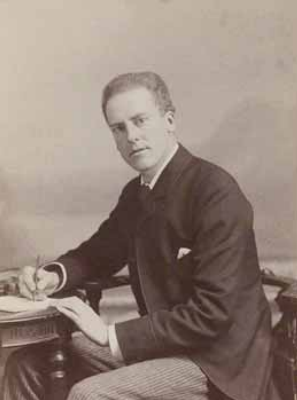
\includegraphics[keepaspectratio]{Section2/Pictures/Karl Pearson.png}}

}

\caption{Karl Pearson (1857-1936)}

\end{figure}%

\section{Introduction}\label{introduction}

Biostatistics is the branch of statistics concerned with the collection,
organization, analysis, interpretation, and presentation of data arising
from the biological and health sciences, including medicine,
epidemiology, public health, biology, and pharmacology. It applies
mathematical and statistical principles to design studies, summarize
data, test hypotheses, and draw valid conclusions about health-related
phenomena --- ranging from the effectiveness of a new drug to the spread
of an infectious disease across a population. At its core, biostatistics
provides the quantitative framework that allows researchers to
distinguish real, meaningful patterns in health data from patterns that
could plausibly have occurred by chance alone.

\subsection{\texorpdfstring{\textbf{Importance of
Biostatistics}}{Importance of Biostatistics}}\label{importance-of-biostatistics}

Think of \textbf{biostatistics} as the backbone of modern medicine and
public health. Without it, most of what we know about diseases,
treatments, and health policies would just be guesswork. Here's why it
matters:

\begin{itemize}
\item
  It builds evidence-based medicine. Every time a doctor prescribes a
  drug based on ``proven effectiveness,'' biostatistics is behind that
  proof.
\item
  It separates real effects from chance. A patient may improve after
  treatment but was it the drug, or just luck? Statistics tells us the
  difference.
\item
  It helps design better research. Before a study even begins,
  biostatistics decides how many people are needed, how they should be
  grouped, and how bias can be avoided.
\item
  It powers public health planning. Governments use disease rates, death
  rates, and survey data to decide where hospitals, vaccines, or health
  campaigns are most needed.
\item
  It ensures new drugs are safe. Regulatory bodies like the FDA require
  statistical proof before approving any new medicine or vaccine.
\item
  It helps track and control epidemics. During outbreaks (like
  COVID-19), statistical models are used to predict spread and evaluate
  control measures.
\item
  It supports personalized treatment. By analyzing patterns in patient
  data, statistics helps doctors predict who is at higher risk and
  tailor treatment accordingly.
\end{itemize}

\subsection{Scope of Biostatistics}\label{scope-of-biostatistics}

Biostatistics is a vast field, touching almost every stage of medical
and health research. Its scope can be understood as a journey from
planning a study to interpreting its results:

\begin{enumerate}
\def\labelenumi{\arabic{enumi}.}
\item
  \textbf{Planning the Study}\\
  Before any data is collected, biostatistics helps decide the best way
  to conduct research --- whether through a cohort study, case-control
  study, or a randomized controlled trial.
\item
  \textbf{Describing the Data}\\
  Once data is collected, it needs to be summarized using averages,
  percentages, and simple charts, so that patterns are easy to see.
\item
  \textbf{Drawing Conclusions}\\
  This is where biostatistics answers the big question: ``Is this result
  real, or just by chance?'' Tools like hypothesis testing, p-values,
  and confidence intervals are used here.
\item
  \textbf{Studying Disease Over Time}\\
  Especially important in chronic disease research which looks at how
  long patients survive, or how long it takes for a disease event to
  occur, using tools like Kaplan-Meier curves.
\item
  \textbf{Following People Over Time (Longitudinal Studies)}\\
  Some diseases develop slowly, so researchers study the same people
  repeatedly over months or years, using specialized statistical models.
\item
  \textbf{Measuring Disease in Populations}\\
  This includes calculating rates of disease occurrence and figuring out
  risk factors --- essential for public health decision-making.
\item
  \textbf{Testing New Treatments}\\
  Biostatistics guides every phase of drug and vaccine testing from
  calculating the right sample size to monitoring safety during the
  trial.
\item
  \textbf{Handling Complex Surveys}\\
  National health surveys often use special sampling methods.
  Biostatistics ensures the results still represent the whole population
  accurately.
\item
  \textbf{Modern Applications}\\
  Today, biostatistics also supports genetic research and machine
  learning tools used for predicting disease risk.
\end{enumerate}

\subsection{Types of Biostatistics}\label{types-of-biostatistics}

Biostatistics is broadly divided into two major types:
\textbf{descriptive} and \textbf{analytical (or inferential)
statistics}.

\subsubsection{Descriptive Statistics}\label{descriptive-statistics-1}

Descriptive statistics refers to the set of methods used to organize,
summarize, and present data in a clear and meaningful way, without
drawing conclusions that go beyond the data itself.

\begin{tcolorbox}[enhanced jigsaw, bottomrule=.15mm, breakable, opacityback=0, toptitle=1mm, titlerule=0mm, bottomtitle=1mm, colback=white, arc=.35mm, rightrule=.15mm, toprule=.15mm, leftrule=.75mm, title=\textcolor{quarto-callout-note-color}{\faInfo}\hspace{0.5em}{Note}, colbacktitle=quarto-callout-note-color!10!white, colframe=quarto-callout-note-color-frame, coltitle=black, left=2mm, opacitybacktitle=0.6]

\textbf{Definition:} Descriptive statistics is the branch of statistics
concerned with \textbf{summarizing, organizing, and presenting} data
using numbers, tables, and graphs, so that the essential features of a
data set can be understood quickly and accurately.

\end{tcolorbox}

Descriptive statistics answers questions such as:

\begin{itemize}
\tightlist
\item
  What is the ``typical'' value in this data set? (measures of central
  tendency)
\item
  How spread out or variable are the observations? (measures of
  dispersion)
\item
  What is the shape of the distribution? Is it symmetric or skewed?
\item
  How are categorical characteristics distributed across groups?
\end{itemize}

Descriptive statistics is contrasted with \textbf{inferential
statistics}, which uses sample data to draw conclusions, make
predictions, or test hypotheses about a larger population (covered later
in this book, beginning with Section 9). Descriptive statistics is
almost always the \textbf{first step} in any statistical analysis before
we can test hypotheses or build models, we must understand the basic
structure of our data.

\textbf{Example (Public Health):} Suppose a health department records
the systolic blood pressure of 200 adults attending a community
screening. Before running any hypothesis test, we would first describe
the data: What is the mean blood pressure? What is the range? How many
participants have blood pressure above 140 mmHg? These are all
descriptive statistics questions.

\textbf{Importance of Descriptive Statistics in Public Health}

Descriptive statistics is foundational to public health practice and
research for several reasons:

\begin{enumerate}
\def\labelenumi{\arabic{enumi}.}
\tightlist
\item
  \textbf{Surveillance:} Public health surveillance systems (e.g.,
  disease registries, vital statistics) rely on descriptive statistics
  --- incidence rates, prevalence, mortality rates --- to monitor
  population health over time.
\item
  \textbf{Needs assessment:} Descriptive statistics identify which
  populations are most affected by a disease or risk factor, guiding
  resource allocation.
\item
  \textbf{Hypothesis generation:} Patterns observed in descriptive data
  (e.g., a cluster of cases in a geographic area) often generate
  hypotheses that are later tested using inferential statistics.
\item
  \textbf{Communication:} Tables, graphs, and summary numbers translate
  complex data into a form that policymakers, clinicians, and the public
  can understand.
\item
  \textbf{Quality control and monitoring:} Hospitals and health systems
  use descriptive statistics (e.g., average length of stay, infection
  rates) to monitor quality of care.
\item
  \textbf{Baseline for comparison:} Before evaluating an intervention,
  descriptive statistics establish a baseline against which
  post-intervention data can be compared.
\end{enumerate}

\textbf{Applications of Descriptive Statistics}

Common applications encountered in biostatistics and epidemiology
include:

\begin{itemize}
\tightlist
\item
  Summarizing \textbf{demographic characteristics} of a study population
  in a ``Table 1'' of a research paper (age, sex, BMI, comorbidities).
\item
  Calculating \textbf{prevalence} and \textbf{incidence} of diseases in
  a population.
\item
  Describing the \textbf{distribution of a biomarker} (e.g., mean and SD
  of fasting glucose in a diabetes study).
\item
  Creating \textbf{epidemic curves} to show the number of new cases of a
  disease over time during an outbreak.
\item
  Producing \textbf{choropleth maps} showing the geographic distribution
  of disease rates.
\item
  Reporting \textbf{vaccination coverage} rates across regions or age
  groups.
\item
  Summarizing \textbf{clinical trial} baseline characteristics before
  comparing treatment arms.
\end{itemize}

\begin{tcolorbox}[enhanced jigsaw, bottomrule=.15mm, breakable, opacityback=0, toptitle=1mm, titlerule=0mm, bottomtitle=1mm, colback=white, arc=.35mm, rightrule=.15mm, toprule=.15mm, leftrule=.75mm, title=\textcolor{quarto-callout-important-color}{\faExclamation}\hspace{0.5em}{Important}, colbacktitle=quarto-callout-important-color!10!white, colframe=quarto-callout-important-color-frame, coltitle=black, left=2mm, opacitybacktitle=0.6]

Descriptive statistics \textbf{describes} the data you have; it does
\textbf{not} allow you to generalize findings to a broader population
with a stated level of confidence which is done by analutical
statistics. That is the role of inferential statistics, introduced
starting in Section 9 of this chapter. Confusing the two --- for
example, treating a sample mean as if it were the population mean
without accounting for sampling variability --- is a common and
important error to avoid.

\end{tcolorbox}

\subsubsection{\texorpdfstring{\textbf{Analytical (inferential)
statistics}}{Analytical (inferential) statistics}}\label{analytical-inferential-statistics}

Analytical statistics by contrast, goes further by using sample data to
draw conclusions, make predictions, or test hypotheses about a larger
population. This branch includes techniques such as hypothesis testing,
confidence interval estimation, regression analysis, survival analysis,
and analysis of variance (ANOVA). Analytical statistics allow
researchers to determine, for example, whether a difference in recovery
rates between two treatment groups is statistically significant or
likely due to chance, or to estimate the strength and direction of the
relationship between a risk factor and a health outcome. Because
analytical methods involve making inferences beyond the observed data,
they require careful attention to study design, sample size, and the
assumptions underlying each statistical test reinforcing why the
historical development of rigorous statistical reasoning, discussed
earlier, remains so central to sound biomedical research today.

\textbf{Importance of Analytical Statistics}

\begin{itemize}
\item
  \textbf{Tests hypotheses scientifically} -- helps confirm or reject
  assumptions using objective, mathematical methods rather than opinion
  or observation alone.
\item
  \textbf{Establishes cause-and-effect relationships} -- helps identify
  whether a risk factor (like smoking) is actually associated with a
  disease outcome (like lung cancer).
\item
  \textbf{Reduces the role of chance and bias} -- through significance
  testing (p-values, confidence intervals), it tells us whether a result
  is likely real or just random variation.
\item
  \textbf{Supports decision-making in medicine} -- guides whether a new
  drug, vaccine, or intervention should be adopted based on solid proof
  of effectiveness.
\item
  \textbf{Allows generalization} -- lets researchers apply conclusions
  from a small sample to a larger population with a known degree of
  confidence.
\item
  \textbf{Strengthens research validity} -- proper analytical methods
  control for confounding factors and bias, making study results more
  trustworthy.
\item
  \textbf{Helps compare groups} -- enables comparison between treatment
  vs.~control groups, exposed vs.~unexposed populations, etc.
\item
  \textbf{Improves resource allocation} -- governments and health
  organizations use analytical findings to prioritize where funding and
  interventions are most needed.
\item
  \textbf{Enables risk prediction} -- helps calculate the probability of
  disease occurrence based on various risk factors.
\item
  \textbf{Forms the basis of evidence-based practice} -- nearly every
  clinical guideline is built on findings validated through analytical
  statistical methods.
\end{itemize}

\textbf{Applications of Analytical Statistics}

\begin{enumerate}
\def\labelenumi{\arabic{enumi}.}
\tightlist
\item
  \textbf{Hypothesis Testing}\\
  Used to test whether a new treatment is significantly better than an
  existing one (e.g., t-test, chi-square test, ANOVA).
\item
  \textbf{Measures of Association}\\
  Calculating relative risk, odds ratio, and attributable risk to
  understand how strongly a factor is linked to a disease.
\item
  \textbf{Regression Analysis}\\
  Used to study the relationship between one outcome and multiple risk
  factors simultaneously (linear, logistic, Cox regression).
\item
  \textbf{Correlation Analysis}\\
  Determines whether two variables (e.g., blood pressure and age) move
  together, and how strongly.
\item
  \textbf{Survival Analysis}\\
  Applied in chronic disease and cancer research to study time-to-event
  outcomes, like time until death or relapse.
\item
  \textbf{Epidemiological Study Designs}\\
  Used in cohort and case-control studies to identify risk factors and
  calculate disease association.
\item
  \textbf{Clinical Trials}\\
  Applied to test whether new drugs or vaccines produce statistically
  significant improvements over placebo or standard treatment.
\item
  \textbf{Quality Control in Public Health Programs}\\
  Used to monitor whether a health intervention (like a vaccination
  drive) is producing the intended effect at a population level.
\item
  \textbf{Predictive Modeling}\\
  Helps forecast disease outbreaks or identify high-risk individuals
  using statistical/machine learning models.
\item
  \textbf{Survey Data Analysis}\\
  Applied in large-scale health surveys to draw valid conclusions while
  accounting for complex sampling designs.
\end{enumerate}

\section{Types of Data}\label{types-of-data}

Data collected in biostatistics and epidemiology generally fall into two
broad categories: \textbf{qualitative (categorical)} and
\textbf{quantitative (numerical)} data.

\begin{Shaded}
\begin{Highlighting}[]
\NormalTok{flowchart TD}
\NormalTok{    A[Types of Data] {-}{-}\textgreater{} B[Qualitative / Categorical]}
\NormalTok{    A {-}{-}\textgreater{} C[Quantitative / Numerical]}
\NormalTok{    B {-}{-}\textgreater{} B1[Nominal]}
\NormalTok{    B {-}{-}\textgreater{} B2[Ordinal]}
\NormalTok{    C {-}{-}\textgreater{} C1[Discrete]}
\NormalTok{    C {-}{-}\textgreater{} C2[Continuous]}
\end{Highlighting}
\end{Shaded}

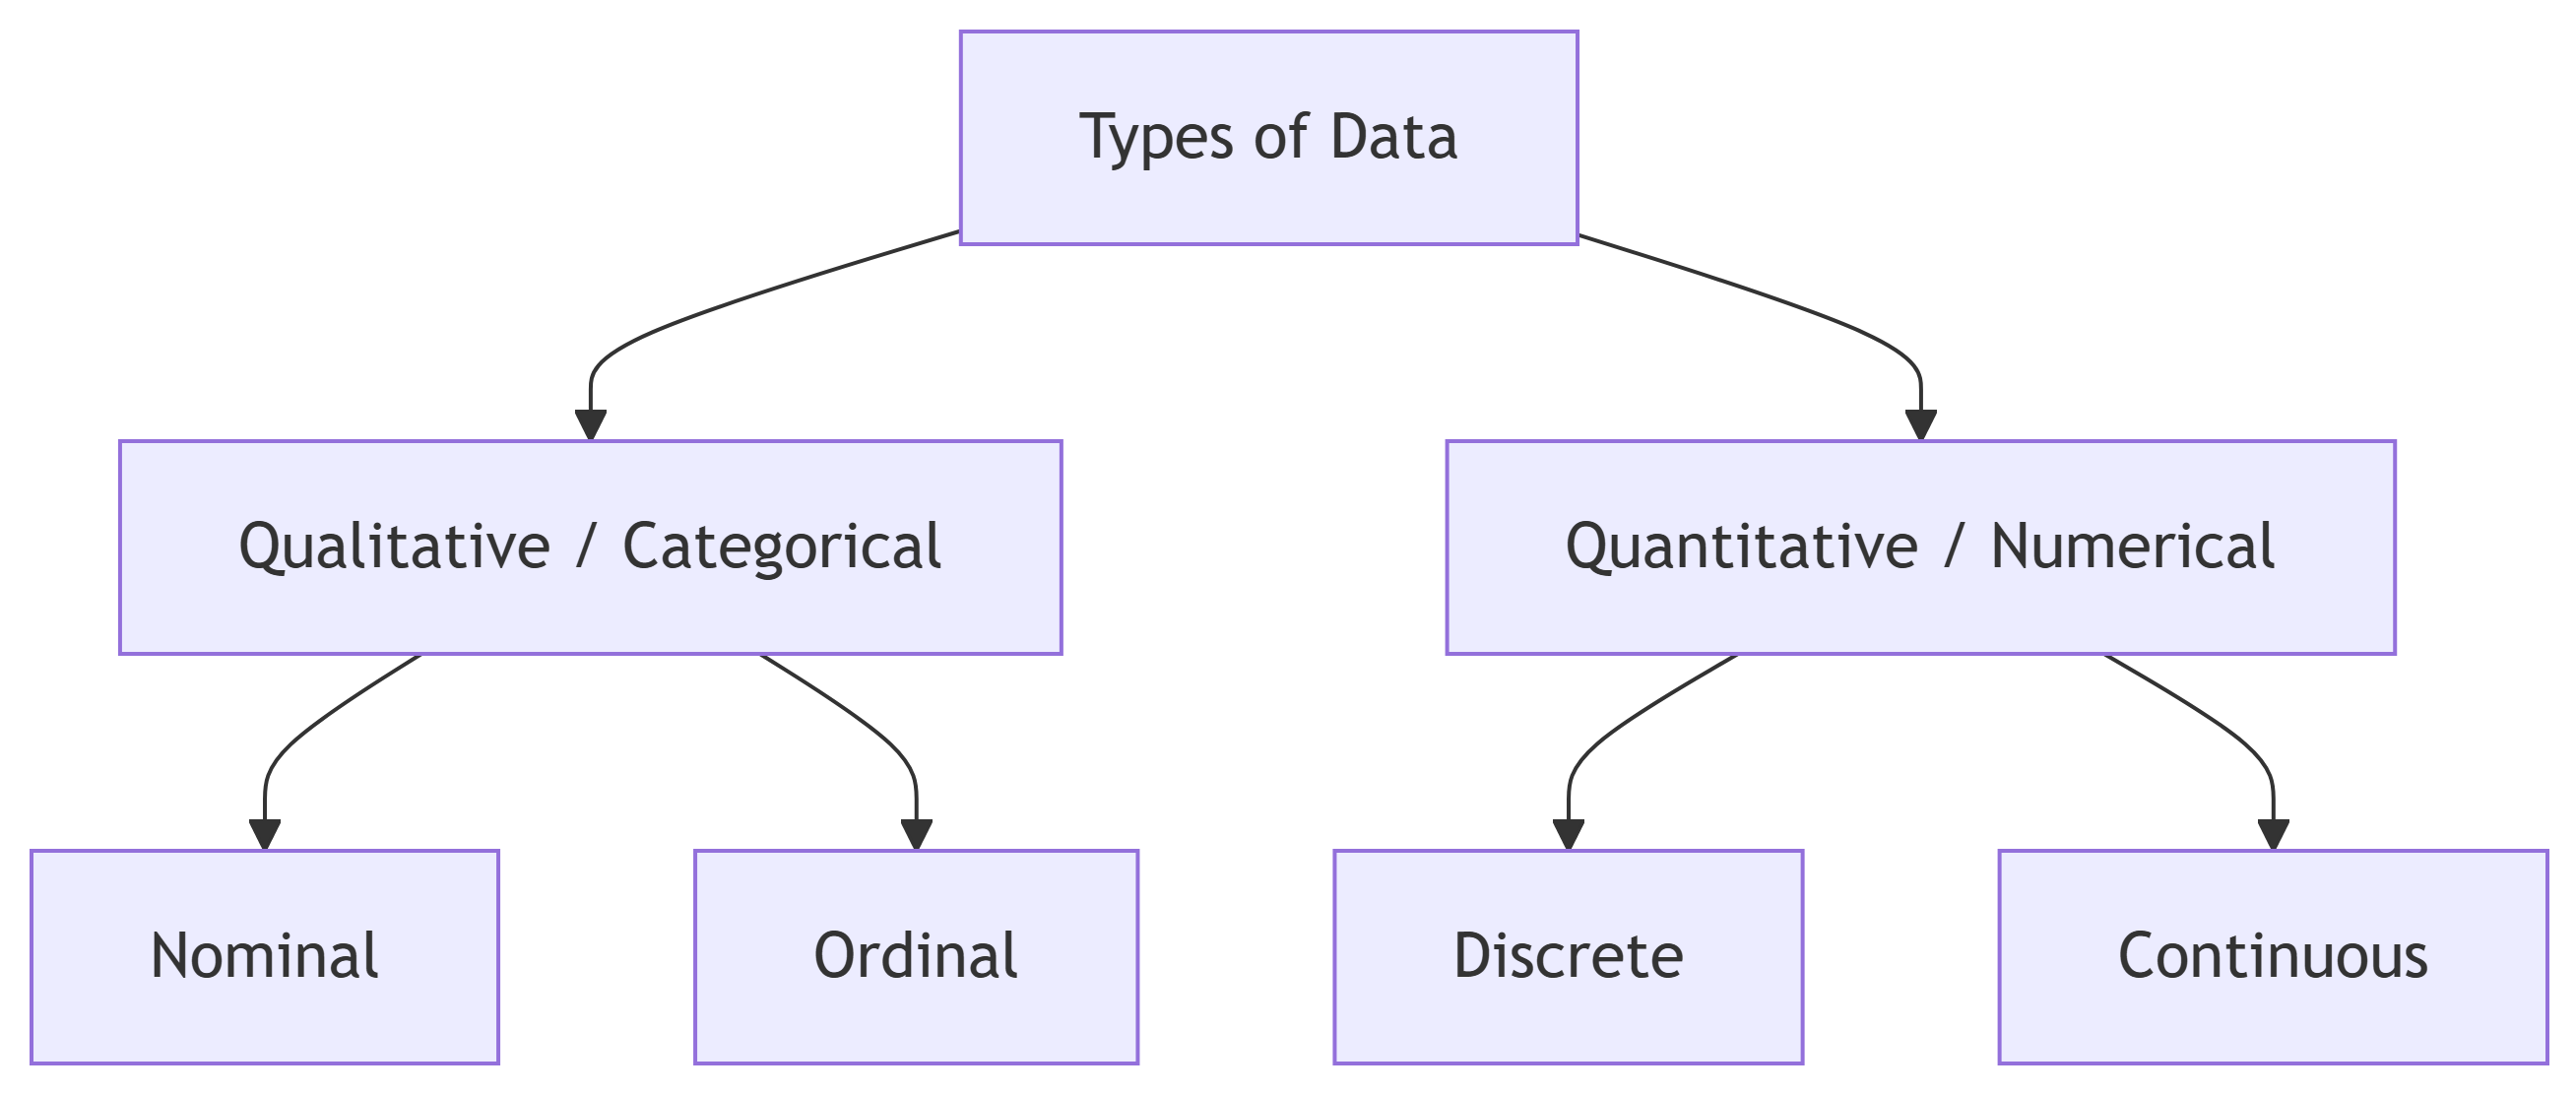
\includegraphics[width=6.82in,height=2.9in]{Section2/01_introduction_descriptive_statistics_files/figure-latex/mermaid-figure-1.png}

\subsection{Qualitative (Categorical)
Data}\label{qualitative-categorical-data}

Categorical data represent characteristics or attributes that place
individuals into groups or categories. They cannot be meaningfully
added, subtracted, or averaged.

\begin{itemize}
\tightlist
\item
  \textbf{Nominal data:} Categories with no inherent order. Example:
  blood type (A, B, AB, O), sex, marital status, country of residence,
  vaccination status (vaccinated/unvaccinated).
\item
  \textbf{Ordinal data:} Categories with a meaningful order, but the
  intervals between categories are not necessarily equal. Example:
  cancer stage (I, II, III, IV), pain severity (mild, moderate, severe),
  socioeconomic status (low, middle, high), Likert scale responses
  (strongly disagree to strongly agree).
\end{itemize}

\subsection{Quantitative (Numerical)
Data}\label{quantitative-numerical-data}

Numerical data represent measurable quantities and can be manipulated
arithmetically.

\begin{itemize}
\tightlist
\item
  \textbf{Discrete data:} Data that can take only specific, countable
  values (usually whole numbers), typically arising from counting.
  Example: number of children per household, number of hospital
  admissions per day, number of new COVID-19 cases per week, parity
  (number of live births).
\item
  \textbf{Continuous data:} Data that can take any value within a range,
  typically arising from measurement. Example: height, weight, blood
  pressure, serum cholesterol level, BMI, gestational age.
\end{itemize}

\begin{tcolorbox}[enhanced jigsaw, bottomrule=.15mm, breakable, opacityback=0, toptitle=1mm, titlerule=0mm, bottomtitle=1mm, colback=white, arc=.35mm, rightrule=.15mm, toprule=.15mm, leftrule=.75mm, title=\textcolor{quarto-callout-tip-color}{\faLightbulb}\hspace{0.5em}{Tip}, colbacktitle=quarto-callout-tip-color!10!white, colframe=quarto-callout-tip-color-frame, coltitle=black, left=2mm, opacitybacktitle=0.6]

A useful rule of thumb: if you can meaningfully ask ``how many?'' the
data are usually discrete; if you can ask ``how much?'' and fractional
values make sense, the data are usually continuous.

\end{tcolorbox}

\textbf{Comparison Table}

\begin{longtable}[]{@{}
  >{\raggedright\arraybackslash}p{(\linewidth - 8\tabcolsep) * \real{0.2000}}
  >{\raggedright\arraybackslash}p{(\linewidth - 8\tabcolsep) * \real{0.2000}}
  >{\raggedright\arraybackslash}p{(\linewidth - 8\tabcolsep) * \real{0.2000}}
  >{\raggedright\arraybackslash}p{(\linewidth - 8\tabcolsep) * \real{0.2000}}
  >{\raggedright\arraybackslash}p{(\linewidth - 8\tabcolsep) * \real{0.2000}}@{}}
\toprule\noalign{}
\begin{minipage}[b]{\linewidth}\raggedright
Feature
\end{minipage} & \begin{minipage}[b]{\linewidth}\raggedright
Nominal
\end{minipage} & \begin{minipage}[b]{\linewidth}\raggedright
Ordinal
\end{minipage} & \begin{minipage}[b]{\linewidth}\raggedright
Discrete
\end{minipage} & \begin{minipage}[b]{\linewidth}\raggedright
Continuous
\end{minipage} \\
\midrule\noalign{}
\endhead
\bottomrule\noalign{}
\endlastfoot
Type & Categorical & Categorical & Numerical & Numerical \\
Order meaningful? & No & Yes & Yes & Yes \\
Arithmetic meaningful? & No & No (generally) & Yes & Yes \\
Example & Blood type & Cancer stage & Number of pregnancies & Blood
pressure \\
\end{longtable}

\section{Population vs.~Sample}\label{population-vs.-sample}

Two of the most fundamental concepts in statistics are the
\textbf{population} and the \textbf{sample}.

\begin{tcolorbox}[enhanced jigsaw, bottomrule=.15mm, breakable, opacityback=0, toptitle=1mm, titlerule=0mm, bottomtitle=1mm, colback=white, arc=.35mm, rightrule=.15mm, toprule=.15mm, leftrule=.75mm, title=\textcolor{quarto-callout-note-color}{\faInfo}\hspace{0.5em}{Note}, colbacktitle=quarto-callout-note-color!10!white, colframe=quarto-callout-note-color-frame, coltitle=black, left=2mm, opacitybacktitle=0.6]

\begin{itemize}
\item
  \textbf{Population:} The complete set of individuals, items, or events
  that share a defining characteristic and about which we want to draw
  conclusions.
\item
  \textbf{Sample:} A subset of the population that is actually observed
  or measured, ideally selected so that it represents the population
  well.

  \pandocbounded{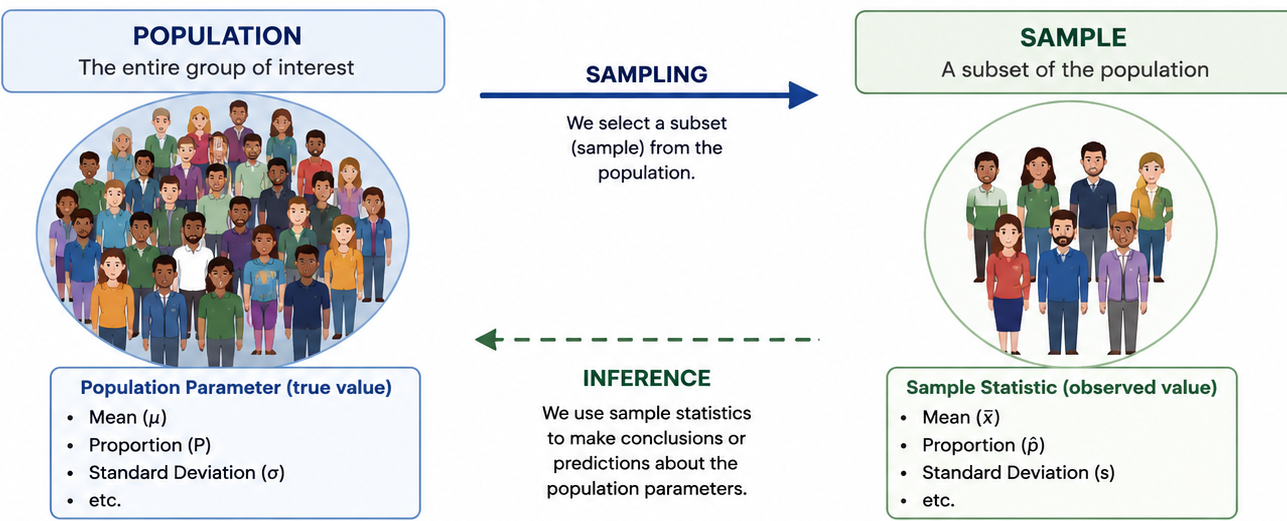
\includegraphics[keepaspectratio]{Section2/Pictures/sample and population.png}}
\end{itemize}

\end{tcolorbox}

We use Greek letters for \textbf{population parameters} (fixed but
usually unknown quantities) and Roman letterss for \textbf{sample
statistics} (computed from data and used to estimate the parameters).

\begin{longtable}[]{@{}lll@{}}
\toprule\noalign{}
Quantity & Population Parameter & Sample Statistic \\
\midrule\noalign{}
\endhead
\bottomrule\noalign{}
\endlastfoot
Mean & \(\mu\) & \(\bar{x}\) \\
Variance & \(\sigma^2\) & \(s^2\) \\
Standard deviation & \(\sigma\) & \(s\) \\
Proportion & \(\pi\) or \(P\) & \(\hat{p}\) \\
Size & \(N\) & \(n\) \\
\end{longtable}

\textbf{Public health example:} A researcher wants to know the average
hemoglobin level of all pregnant women in a country (the population,
size \(N\)). Since testing every pregnant woman is infeasible, a
\textbf{sample} of \(n = 500\) pregnant women is selected from antenatal
clinics, and the sample mean \(\bar{x}\) is used to \textbf{estimate}
the unknown population mean \(\mu\).

Why do we sample instead of studying the whole population?

\begin{itemize}
\tightlist
\item
  \textbf{Feasibility:} Populations are often too large (e.g., all
  adults in a country).
\item
  \textbf{Cost and time:} Surveying an entire population is expensive
  and slow.
\item
  \textbf{Practicality:} Some measurements are destructive or invasive
  (e.g., biopsy), so testing everyone is not possible.
\item
  \textbf{Accuracy:} A well-designed sample with careful data collection
  can sometimes yield more accurate information than a poorly conducted
  census.
\end{itemize}

For a sample to give a good estimate of the population, it should
ideally be selected using a method that avoids \textbf{selection bias},
such as simple random sampling, stratified sampling, or cluster
sampling.

\section{Variables}\label{variables}

A \textbf{variable} is any characteristic, number, or quantity that can
be measured or counted and that can differ from one individual (or
observation) to another.

\subsection{Classification of
Variables}\label{classification-of-variables}

\begin{Shaded}
\begin{Highlighting}[]
\NormalTok{flowchart TD}
\NormalTok{    V[Variables] {-}{-}\textgreater{} Q[Quantitative]}
\NormalTok{    V {-}{-}\textgreater{} C[Qualitative]}
\NormalTok{    Q {-}{-}\textgreater{} QD[Discrete]}
\NormalTok{    Q {-}{-}\textgreater{} QC[Continuous]}
\NormalTok{    C {-}{-}\textgreater{} CN[Nominal]}
\NormalTok{    C {-}{-}\textgreater{} CO[Ordinal]}
\NormalTok{    V {-}{-}\textgreater{} R[By Role in Analysis]}
\NormalTok{    R {-}{-}\textgreater{} R1[Independent / Exposure Variable]}
\NormalTok{    R {-}{-}\textgreater{} R2[Dependent / Outcome Variable]}
\NormalTok{    R {-}{-}\textgreater{} R3[Confounding Variable]}
\end{Highlighting}
\end{Shaded}

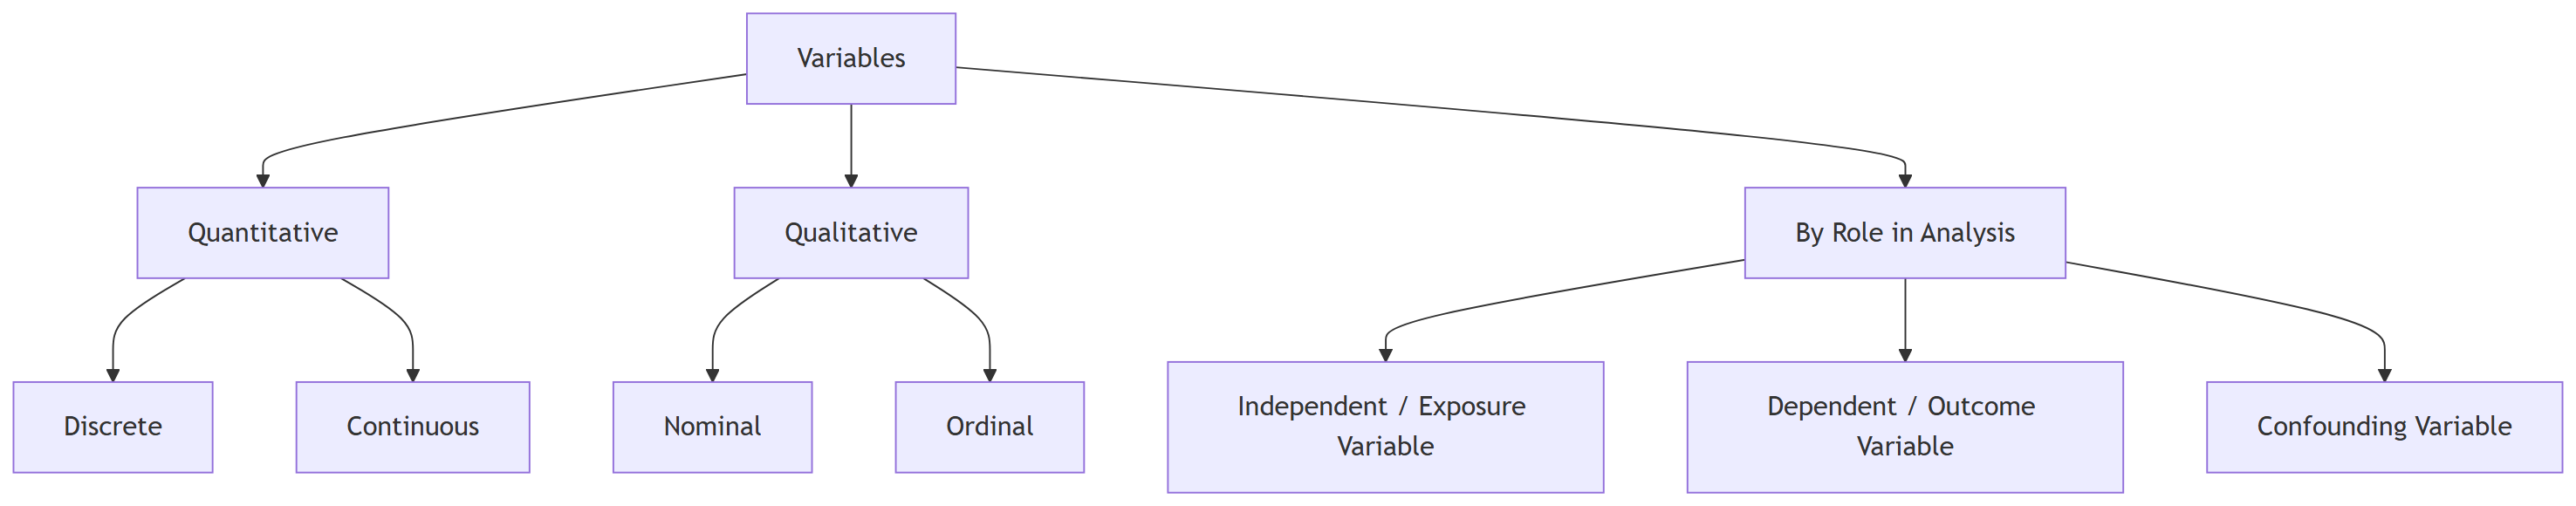
\includegraphics[width=16.01in,height=3.15in]{Section2/01_introduction_descriptive_statistics_files/figure-latex/mermaid-figure-2.png}

\begin{itemize}
\tightlist
\item
  \textbf{Independent variable (exposure/predictor):} The variable
  believed to influence or predict the outcome. Example: smoking status.
\item
  \textbf{Dependent variable (outcome/response):} The variable being
  predicted or explained. Example: lung cancer status.
\item
  \textbf{Confounding variable:} A variable associated with both the
  exposure and the outcome that can distort the observed association if
  not controlled for. Example: age as a confounder in the relationship
  between physical activity and heart disease.
\end{itemize}

\textbf{Public health example:} In a study of the relationship between
air pollution (independent variable measured as PM2.5 concentration, a
continuous variable) and asthma attacks (dependent variable, a discrete
count), age and smoking status might act as confounding variables.

\section{Scales of Measurement}\label{scales-of-measurement-1}

Stanley Smith Stevens (1946) classified measurement into four
scales(Stevens 1946). Understanding the scale of measurement of a
variable is essential because it determines which descriptive statistics
and which statistical tests are appropriate.

\begin{longtable}[]{@{}
  >{\raggedright\arraybackslash}p{(\linewidth - 10\tabcolsep) * \real{0.1667}}
  >{\raggedright\arraybackslash}p{(\linewidth - 10\tabcolsep) * \real{0.1667}}
  >{\raggedright\arraybackslash}p{(\linewidth - 10\tabcolsep) * \real{0.1667}}
  >{\raggedright\arraybackslash}p{(\linewidth - 10\tabcolsep) * \real{0.1667}}
  >{\raggedright\arraybackslash}p{(\linewidth - 10\tabcolsep) * \real{0.1667}}
  >{\raggedright\arraybackslash}p{(\linewidth - 10\tabcolsep) * \real{0.1667}}@{}}
\toprule\noalign{}
\begin{minipage}[b]{\linewidth}\raggedright
Scale
\end{minipage} & \begin{minipage}[b]{\linewidth}\raggedright
Order?
\end{minipage} & \begin{minipage}[b]{\linewidth}\raggedright
Equal intervals?
\end{minipage} & \begin{minipage}[b]{\linewidth}\raggedright
True zero?
\end{minipage} & \begin{minipage}[b]{\linewidth}\raggedright
Allowed operations
\end{minipage} & \begin{minipage}[b]{\linewidth}\raggedright
Examples
\end{minipage} \\
\midrule\noalign{}
\endhead
\bottomrule\noalign{}
\endlastfoot
\textbf{Nominal} & No & No & No & Counting, mode, frequencies & Blood
type, sex, ethnicity \\
\textbf{Ordinal} & Yes & No & No & Median, percentiles, ranking & Cancer
stage, pain scale \\
\textbf{Interval} & Yes & Yes & No (arbitrary zero) & Mean, SD,
addition/subtraction & Temperature (°C), IQ score \\
\textbf{Ratio} & Yes & Yes & Yes (true zero) & All arithmetic, including
ratios & Weight, height, age, blood pressure \\
\end{longtable}

\begin{tcolorbox}[enhanced jigsaw, bottomrule=.15mm, breakable, opacityback=0, toptitle=1mm, titlerule=0mm, bottomtitle=1mm, colback=white, arc=.35mm, rightrule=.15mm, toprule=.15mm, leftrule=.75mm, title=\textcolor{quarto-callout-tip-color}{\faLightbulb}\hspace{0.5em}{Tip}, colbacktitle=quarto-callout-tip-color!10!white, colframe=quarto-callout-tip-color-frame, coltitle=black, left=2mm, opacitybacktitle=0.6]

A simple test for \textbf{ratio scale}: does ``zero'' mean ``none of the
quantity,'' and does it make sense to say ``20 kg is twice as heavy as
10 kg''? If yes, it is a ratio scale. Temperature in Celsius fails this
test (0°C is not ``no temperature,'' and 20°C is not ``twice as hot'' as
10°C), so it is only an interval scale.

\end{tcolorbox}

Nominal and ordinal scales are collectively referred to as
\textbf{categorical}, while interval and ratio scales are collectively
referred to as \textbf{numerical/quantitative}. Most public health and
clinical measurements (weight, blood pressure, cell counts, survival
time) are on the ratio scale.

\section{Summary}\label{summary}

\begin{itemize}
\tightlist
\item
  Descriptive statistics organizes, summarizes, and presents data using
  numbers, tables, and graphs.
\item
  Data are broadly classified as \textbf{qualitative} (nominal, ordinal)
  or \textbf{quantitative} (discrete, continuous).
\item
  A \textbf{population} is the complete group of interest; a
  \textbf{sample} is a subset used to estimate population
  characteristics.
\item
  \textbf{Variables} may serve as independent, dependent, or confounding
  variables in an analysis.
\item
  The \textbf{scale of measurement} (nominal, ordinal, interval, ratio)
  determines which statistical summaries and tests are valid.
\item
  Descriptive statistics underlies nearly every activity in public
  health practice, from surveillance to communication of results.
\end{itemize}

The next section will build on these foundations by covering
\textbf{measures of central tendency} in depth.

\section{References}\label{references-1}

\chapter{Measures of Central
Tendency}\label{measures-of-central-tendency}

\section{Introduction}\label{introduction-1}

A \textbf{measure of central tendency} is a single value that attempts
to describe a data set by identifying the ``center'' or ``typical''
value of the distribution. The three classical measures are the
\textbf{mean}, \textbf{median}, and \textbf{mode}; we also cover
\textbf{quartiles}, \textbf{percentiles}, and \textbf{deciles}, which
are measures of \emph{position} closely related to the median.

Throughout this section we will use three running data sets so every
formula can be demonstrated with a full, step-by-step manual
calculation:

\begin{itemize}
\item
  \textbf{Dataset A (raw/ungrouped data):} Fasting blood glucose (mg/dL)
  of 11 patients attending a diabetes clinic:

  \texttt{88,\ 92,\ 95,\ 98,\ 101,\ 104,\ 108,\ 112,\ 118,\ 125,\ 250}
\item
  \textbf{Dataset B (frequency table / discrete data):} Number of
  children in 40 households in a village survey.

  \begin{longtable}[]{@{}ll@{}}
  \toprule\noalign{}
  Number of children (\(x\)) & Frequency (\(f\)) \\
  \midrule\noalign{}
  \endhead
  \bottomrule\noalign{}
  \endlastfoot
  0 & 6 \\
  1 & 10 \\
  2 & 14 \\
  3 & 7 \\
  4 & 3 \\
  \textbf{Total} & 40 \\
  \end{longtable}
\item
  \textbf{Data Set C (grouped frequency distribution):} Age (in years)
  of 50 patients admitted with hypertension, grouped into class
  intervals.

  \begin{longtable}[]{@{}ll@{}}
  \toprule\noalign{}
  Class interval & Frequency (\(f\)) \\
  \midrule\noalign{}
  \endhead
  \bottomrule\noalign{}
  \endlastfoot
  30--39 & 4 \\
  40--49 & 9 \\
  50--59 & 15 \\
  60--69 & 13 \\
  70--79 & 7 \\
  80--89 & 2 \\
  \textbf{Total} & 50 \\
  \end{longtable}
\end{itemize}

\section{The Arithmetic Mean}\label{the-arithmetic-mean}

\subsection{Definition}\label{definition}

The \textbf{arithmetic mean} (commonly just called ``the mean'' or
``average'') is the sum of all observations divided by the number of
observations.

\subsection{Formula}\label{formula}

For a population of size \(N\): \[\mu = \frac{\sum_{i=1}^{N} X_i}{N}\]

For a sample of size \(n\): \[\bar{x} = \frac{\sum_{i=1}^{n} x_i}{n}\]

\subsection{Manual Calculation}\label{manual-calculation}

\subsubsection{A. Raw (Ungrouped) Data}\label{a.-raw-ungrouped-data}

Using Data Set A (fasting glucose, mg/dL): 88, 92, 95, 98, 101, 104,
108, 112, 118, 125, 250 (\(n = 11\))

\textbf{Step 1.} Sum all observations:
\[\sum x_i = 88+92+95+98+101+104+108+112+118+125+250 = 1291\]

\textbf{Step 2.} Divide by \(n\):
\[\bar{x} = \frac{1291}{11} = 117.4 \text{ mg/dL}\]

Notice that the single extreme value (250 mg/dL, representing an
undiagnosed diabetic outlier) pulls the mean upward --- this illustrates
the mean's \textbf{sensitivity to outliers}, discussed further below.

\subsubsection{B. Frequency Table (Ungrouped, Discrete
Data)}\label{b.-frequency-table-ungrouped-discrete-data}

Data Set B --- number of children (\(x\)) per household, surveyed in 40
households:

\begin{longtable}[]{@{}lll@{}}
\toprule\noalign{}
Number of children (\(x\)) & Frequency (\(f\)) & \(f \times x\) \\
\midrule\noalign{}
\endhead
\bottomrule\noalign{}
\endlastfoot
0 & 6 & 0 \\
1 & 10 & 10 \\
2 & 14 & 28 \\
3 & 7 & 21 \\
4 & 3 & 12 \\
\textbf{Total} & \(n = \sum f = 40\) & \(\sum fx = 71\) \\
\end{longtable}

\textbf{Formula:} \(\bar{x} = \dfrac{\sum f_i x_i}{\sum f_i}\)

\textbf{Step 1.} Compute \(f \times x\) for each row (shown above).

\textbf{Step 2.} Sum the \(fx\) column:
\(\sum fx = 0+10+28+21+12 = 71\).

\textbf{Step 3.} Sum the frequency column:
\(\sum f = 6+10+14+7+3 = 40\).

\textbf{Step 4.} Divide:
\[\bar{x} = \frac{71}{40} = 1.775 \approx 1.8 \text{ children per household}\]

\subsection{C. Grouped Frequency
Distribution}\label{c.-grouped-frequency-distribution}

Data Set C is a age (in years) of 50 hypertension patients:

\begin{longtable}[]{@{}
  >{\raggedright\arraybackslash}p{(\linewidth - 6\tabcolsep) * \real{0.2319}}
  >{\raggedright\arraybackslash}p{(\linewidth - 6\tabcolsep) * \real{0.2319}}
  >{\raggedright\arraybackslash}p{(\linewidth - 6\tabcolsep) * \real{0.2464}}
  >{\raggedright\arraybackslash}p{(\linewidth - 6\tabcolsep) * \real{0.2899}}@{}}
\toprule\noalign{}
\begin{minipage}[b]{\linewidth}\raggedright
Class interval
\end{minipage} & \begin{minipage}[b]{\linewidth}\raggedright
Midpoint (\(m\))
\end{minipage} & \begin{minipage}[b]{\linewidth}\raggedright
Frequency (\(f\))
\end{minipage} & \begin{minipage}[b]{\linewidth}\raggedright
\(f \times m\)
\end{minipage} \\
\midrule\noalign{}
\endhead
\bottomrule\noalign{}
\endlastfoot
30--39 & 34.5 & 4 & 138.0 \\
40--49 & 44.5 & 9 & 400.5 \\
50--59 & 54.5 & 15 & 817.5 \\
60--69 & 64.5 & 13 & 838.5 \\
70--79 & 74.5 & 7 & 521.5 \\
80--89 & 84.5 & 2 & 169.0 \\
\textbf{Total} & - & \(n = 50\) & \(\sum fm = 2885.0\) \\
\end{longtable}

\textbf{Formula:} \(\bar{x} = \dfrac{\sum f_i m_i}{\sum f_i}\), where
\(m_i\) is the midpoint of each class.

\textbf{Step 1.} Find the midpoint of each class:
\(m = \dfrac{\text{lower limit} + \text{upper limit}}{2}\). For 30--39:
\(m = (30+39)/2 = 34.5\) (using continuous class boundaries 29.5--39.5
is also acceptable and gives the same midpoint here). \textbf{Step 2.}
Multiply each midpoint by its frequency (\(f \times m\)), shown above.
\textbf{Step 3.} Sum the \(fm\) column: \(2885.0\). \textbf{Step 4.}
Divide by total frequency:
\[\bar{x} = \frac{2885.0}{50} = 57.7 \text{ years}\]

\begin{tcolorbox}[enhanced jigsaw, bottomrule=.15mm, breakable, opacityback=0, toptitle=1mm, titlerule=0mm, bottomtitle=1mm, colback=white, arc=.35mm, rightrule=.15mm, toprule=.15mm, leftrule=.75mm, title=\textcolor{quarto-callout-important-color}{\faExclamation}\hspace{0.5em}{Important}, colbacktitle=quarto-callout-important-color!10!white, colframe=quarto-callout-important-color-frame, coltitle=black, left=2mm, opacitybacktitle=0.6]

The grouped mean is an \textbf{approximation} because individual raw
values inside each class are unknown; we assume every observation in a
class is located at the midpoint. This assumption introduces a small
amount of \textbf{grouping error}.

\end{tcolorbox}

\subsection{Interpretation}\label{interpretation}

The arithmetic mean represents the ``balance point'' of the data. If the
data were weights on a see-saw, the mean is where it would balance.

\subsection{Advantages}\label{advantages}

\begin{itemize}
\tightlist
\item
  Uses every observation in the data set.
\item
  Algebraically tractable (has well-defined mathematical properties,
  e.g., \(\sum (x_i - \bar{x}) = 0\)), making it the basis for further
  statistics (variance, regression, etc.).
\item
  Familiar and easy to interpret.
\item
  Stable from sample to sample (least sampling variability among the
  three central tendency measures, under normality).
\end{itemize}

\subsection{Disadvantages}\label{disadvantages}

\begin{itemize}
\tightlist
\item
  Highly sensitive to \textbf{outliers and skewed data} (as shown above,
  one value of 250 pulled the mean far above where most data points
  lie).
\item
  Cannot be computed for open-ended class intervals or for
  nominal/ordinal data.
\item
  Can produce a value that does not correspond to any actual observation
  (e.g., ``1.8 children''), which may seem unnatural.
\end{itemize}

\subsection{Appropriate Use}\label{appropriate-use}

The mean is most appropriate when data are \textbf{symmetric
(approximately normally distributed)} and free of major outliers, and
when the variable is measured on an \textbf{interval or ratio scale}.

\subsection{Public Health Example}\label{public-health-example}

The mean is used to report the \textbf{average birth weight} of newborns
in a hospital, the \textbf{mean systolic blood pressure} in a screened
population, or the \textbf{mean length of hospital stay} for a given
diagnosis.

\section{Weighted Mean}\label{weighted-mean}

\subsection{Definition}\label{definition-1}

The \textbf{weighted mean} is a generalization of the arithmetic mean in
which each observation is multiplied by a weight reflecting its relative
importance, rather than being treated equally.

\subsection{Formula}\label{formula-1}

\[\bar{x}_w = \frac{\sum_{i=1}^{k} w_i x_i}{\sum_{i=1}^{k} w_i}\]

where \(w_i\) is the weight assigned to value \(x_i\).

\subsection{Worked Example (Public
Health)}\label{worked-example-public-health}

A district's overall infant mortality rate (IMR) is calculated by
combining IMRs from three sub-districts, weighted by the number of live
births in each (not by simply averaging the three rates):

\begin{longtable}[]{@{}
  >{\raggedright\arraybackslash}p{(\linewidth - 6\tabcolsep) * \real{0.2500}}
  >{\raggedright\arraybackslash}p{(\linewidth - 6\tabcolsep) * \real{0.2500}}
  >{\raggedright\arraybackslash}p{(\linewidth - 6\tabcolsep) * \real{0.2500}}
  >{\raggedright\arraybackslash}p{(\linewidth - 6\tabcolsep) * \real{0.2500}}@{}}
\toprule\noalign{}
\begin{minipage}[b]{\linewidth}\raggedright
Sub-district
\end{minipage} & \begin{minipage}[b]{\linewidth}\raggedright
IMR per 1000 live births (\(x\))
\end{minipage} & \begin{minipage}[b]{\linewidth}\raggedright
Live births (weight \(w\))
\end{minipage} & \begin{minipage}[b]{\linewidth}\raggedright
\(w \times x\)
\end{minipage} \\
\midrule\noalign{}
\endhead
\bottomrule\noalign{}
\endlastfoot
A & 25 & 2000 & 50,000 \\
B & 40 & 500 & 20,000 \\
C & 18 & 3500 & 63,000 \\
\textbf{Total} & & \(\sum w = 6000\) & \(\sum wx = 133{,}000\) \\
\end{longtable}

\textbf{Step 1.} Multiply each rate by its weight (live births): shown
above. \textbf{Step 2.} Sum the weighted values: \(133{,}000\).
\textbf{Step 3.} Sum the weights: \(6000\). \textbf{Step 4.} Divide:
\[\bar{x}_w = \frac{133{,}000}{6000} = 22.17 \text{ per } 1000 \text{ live births}\]

Notice that the naive (unweighted) average of 25, 40, and 18 would be
\(27.7\) --- quite different, and misleading, because it ignores that
sub-district B has far fewer births and should count less toward the
district total.

\subsection{Interpretation}\label{interpretation-1}

The weighted mean reflects the true overall rate/value when subgroups
contribute unequally to the total.

\subsection{Advantages}\label{advantages-1}

\begin{itemize}
\tightlist
\item
  Accounts for differing sample sizes or importance across subgroups.
\item
  Prevents small subgroups from distorting the overall estimate.
\end{itemize}

\subsection{Disadvantages}\label{disadvantages-1}

\begin{itemize}
\tightlist
\item
  Requires accurate and appropriate weights; incorrect weights produce a
  misleading result.
\item
  More complex to compute and explain than the simple mean.
\end{itemize}

\subsection{Appropriate Use}\label{appropriate-use-1}

Used whenever combining rates or averages from groups of unequal size.
Standardized mortality/morbidity rates, meta-analysis of study results
(weighted by sample size or inverse variance), grade point averages
(weighted by credit hours).

\subsection{Public Health Example}\label{public-health-example-1}

\textbf{Age-standardized mortality rates}, which combine age-specific
death rates using a standard population's age distribution as weights,
so that mortality rates can be fairly compared across populations with
different age structures.

\section{Geometric Mean}\label{geometric-mean-1}

\subsection{Definition}\label{definition-2}

The \textbf{geometric mean (GM)} is the \(n\)-th root of the product of
\(n\) observations. It is used for data that grow
\textbf{multiplicatively} (e.g., rates of change, ratios, or
log-normally distributed data such as antibody titers).

\subsection{Formula}\label{formula-2}

\[GM = \sqrt[n]{x_1 \times x_2 \times \cdots \times x_n} = \left( \prod_{i=1}^n x_i \right)^{1/n}\]

Equivalently, using logarithms (easier for manual calculation with many
observations):
\[GM = \exp\left( \frac{\sum_{i=1}^{n} \ln(x_i)}{n} \right)\]

\subsection{Manual Calculation}\label{manual-calculation-1}

Suppose antibody titers (reciprocal dilution) from 4 patients after
vaccination are: 8, 16, 32, 128.

\textbf{Step 1.} Multiply all values:
\(8 \times 16 \times 32 \times 128 = 524{,}288\). \textbf{Step 2.} Take
the \(n\)-th root (\(n = 4\)): \[GM = \sqrt[4]{524{,}288} = 26.9\]

\textbf{Verification using logarithms:} \(\ln 8 = 2.079\),
\(\ln 16 = 2.773\), \(\ln 32 = 3.466\), \(\ln 128 = 4.852\). Sum
\(= 13.17\). Mean of logs \(= 13.17/4 = 3.29\). \(GM = e^{3.29} = 26.9\)
✓.

Compare this to the arithmetic mean of the same data:
\(\bar{x} = (8+16+32+128)/4 = 46\). The geometric mean (26.9) is always
\(\le\) the arithmetic mean (46) for positive data, and is much less
influenced by the largest value (128).

\subsection{Interpretation}\label{interpretation-2}

The geometric mean represents the central tendency of
\textbf{multiplicative or exponential} processes; it is the appropriate
``average'' when data are ratios, growth rates, or span several orders
of magnitude.

\subsection{Advantages}\label{advantages-2}

\begin{itemize}
\tightlist
\item
  Less affected by extreme high values than the arithmetic mean (dampens
  the effect of outliers because it operates on a log scale).
\item
  Appropriate for \textbf{log-normally distributed} data (very common in
  laboratory/biological measurements such as titers, viral loads, and
  PCR cycle thresholds).
\item
  Useful for averaging ratios, rates of growth, or index numbers.
\end{itemize}

\subsection{Disadvantages}\label{disadvantages-2}

\begin{itemize}
\tightlist
\item
  Undefined if any observation is zero or negative.
\item
  More difficult to compute manually and less intuitive to interpret
  than the arithmetic mean.
\item
  Not appropriate for additive data.
\end{itemize}

\subsection{Appropriate Use}\label{appropriate-use-2}

Used for \textbf{serial dilution titers}, \textbf{viral load and
antibody data}, growth rates of populations or bacterial cultures, and
any positively skewed, log-normal biological data.

\subsection{Public Health Example}\label{public-health-example-2}

Reporting the \textbf{geometric mean antibody titer} post-vaccination in
a clinical trial, or the \textbf{geometric mean viral load} in an HIV
cohort, standard practice in immunology and virology because titers are
log-normally distributed.

\section{Harmonic Mean}\label{harmonic-mean-1}

\subsection{Definition}\label{definition-3}

The \textbf{harmonic mean (HM)} is the reciprocal of the arithmetic mean
of the reciprocals of the observations. It is most appropriate for
averaging \textbf{rates} (e.g., speeds, rates per unit time) when the
numerator is fixed.

\subsection{Formula}\label{formula-3}

\[HM = \frac{n}{\sum_{i=1}^{n} \frac{1}{x_i}}\]

\subsection{Manual Calculation}\label{manual-calculation-2}

Suppose three health workers screen patients at rates of 20, 30, and 60
patients per hour, and each worked for the \textbf{same total number of
patients screened} (not the same amount of time). Find the average
screening rate.

\textbf{Step 1.} Take the reciprocal of each rate: \(1/20 = 0.0500\),
\(1/30 = 0.0333\), \(1/60 = 0.0167\).

\textbf{Step 2.} Sum the reciprocals: \(0.0500+0.0333+0.0167 = 0.1000\).

\textbf{Step 3.} Divide \(n\) by this sum:
\[HM = \frac{3}{0.1000} = 30 \text{ patients/hour}\]

Note that the arithmetic mean of the same three rates would be
\((20+30+60)/3 = 36.7\), which would \textbf{overstate} the true average
rate when the underlying quantity (patients screened) is fixed, not the
time.

\subsection{Interpretation}\label{interpretation-3}

The harmonic mean gives the correct ``average rate'' when combining
rates that share a common numerator (e.g., a fixed distance, fixed
number of patients, or fixed dose).

\subsection{Advantages}\label{advantages-3}

\begin{itemize}
\tightlist
\item
  Correct choice for averaging rates and ratios where the denominator
  varies.
\item
  Strongly dampens the influence of large values --- most conservative
  of the three Pythagorean means (\(HM \le GM \le AM\)).
\end{itemize}

\subsection{Disadvantages}\label{disadvantages-3}

\begin{itemize}
\tightlist
\item
  Undefined if any value is zero.
\item
  Rarely used and often misunderstood; easy to apply incorrectly.
\item
  Heavily influenced by small values.
\end{itemize}

\subsection{Appropriate Use}\label{appropriate-use-3}

Used when averaging \textbf{rates} such as speed, dose per kilogram, or
performance rates, particularly when the events being counted (not the
time) are held constant.

\subsection{Public Health Example}\label{public-health-example-3}

Calculating the average \textbf{turnaround time rate} for laboratory
tests processed at different rates by different technicians, or
combining rates in \textbf{person-time incidence} calculations.

\section{Relationship Among the Three
Means}\label{relationship-among-the-three-means}

For any set of positive numbers that are not all identical:
\[HM \le GM \le AM\]

The three means are equal only when all observations are identical.

\section{The Median}\label{the-median}

\subsection{Definition}\label{definition-4}

The \textbf{median} is the middle value of a data set when the
observations are arranged in ascending (or descending) order. It divides
the data into two equal halves: 50\% of observations lie at or below the
median, and 50\% lie at or above it.

\subsection{Formula}\label{formula-4}

For raw/ungrouped data with \(n\) observations sorted in order:

\begin{itemize}
\tightlist
\item
  If \(n\) is \textbf{odd}: Median \(= x_{\left(\frac{n+1}{2}\right)}\)
\item
  If \(n\) is \textbf{even}: Median
  \(= \dfrac{x_{(n/2)} + x_{(n/2+1)}}{2}\)
\end{itemize}

For grouped data:
\[\text{Median} = L + \left( \frac{\frac{n}{2} - CF}{f} \right) \times h\]

where \(L\) = lower boundary of the median class, \(n\) = total
frequency, \(CF\) = cumulative frequency before the median class, \(f\)
= frequency of the median class, \(h\) = class width.

\subsection{Manual Calculation}\label{manual-calculation-3}

\subsection{A. Raw Data}\label{a.-raw-data}

Dataset A sorted: 88, 92, 95, 98, 101, 104, 108, 112, 118, 125, 250
(\(n = 11\), odd)

\textbf{Step 1.} Confirm data are sorted (already sorted above).

\textbf{Step 2.} Since \(n = 11\) is odd, the median is the
\(\left(\frac{11+1}{2}\right) = 6^{th}\) value.

\textbf{Step 3.} Count to the 6th value: 88(1), 92(2), 95(3), 98(4),
101(5), \textbf{104(6)}. \[\text{Median} = 104 \text{ mg/dL}\]

Notice the median (104) is much closer to where most of the data lie
than the mean (117.4). Here, the median is \textbf{not} pulled by the
outlier of 250.

\subsection{B. Frequency Table}\label{b.-frequency-table}

Data Set B (number of children per household):

\begin{longtable}[]{@{}lll@{}}
\toprule\noalign{}
\(x\) & \(f\) & Cumulative frequency (\(CF\)) \\
\midrule\noalign{}
\endhead
\bottomrule\noalign{}
\endlastfoot
0 & 6 & 6 \\
1 & 10 & 16 \\
2 & 14 & 30 \\
3 & 7 & 37 \\
4 & 3 & 40 \\
\end{longtable}

\textbf{Step 1.} Build the cumulative frequency column (shown above).

\textbf{Step 2.} With \(n = 40\) (even), the median position is the
average of the \(20^{th}\) and \(21^{st}\) values.

\textbf{Step 3.} Locate these positions using \(CF\): the
\(17^{th}\)--\(30^{th}\) values all equal 2 (since \(CF\) jumps from 16
to 30 at \(x=2\)). Both the \(20^{th}\) and \(21^{st}\) values fall in
this range.

\textbf{Step 4.} Calculation
\[\text{Median} = \frac{2+2}{2} = 2 \text{ children}\]

\subsection{C. Grouped Frequency
Distribution}\label{c.-grouped-frequency-distribution-1}

Data Set C (age of 50 hypertension patients):

\begin{longtable}[]{@{}lll@{}}
\toprule\noalign{}
Class & \(f\) & \(CF\) \\
\midrule\noalign{}
\endhead
\bottomrule\noalign{}
\endlastfoot
30--39 & 4 & 4 \\
40--49 & 9 & 13 \\
50--59 & 15 & 28 \\
60--69 & 13 & 41 \\
70--79 & 7 & 48 \\
80--89 & 2 & 50 \\
\end{longtable}

\textbf{Step 1.} \(n/2 = 50/2 = 25\).

\textbf{Step 2.} Find the median class: the class where the cumulative
frequency first reaches/exceeds 25. That is the \textbf{50--59} class
(\(CF\) jumps from 13 to 28).

\textbf{Step 3.} Identify: \(L = 49.5\) (lower boundary), \(CF = 13\)
(cumulative frequency \emph{before} median class), \(f = 15\) (frequency
of median class), \(h = 10\) (class width).

\textbf{Step 4.} Apply the formula:
\[\text{Median} = 49.5 + \left( \frac{25 - 13}{15} \right) \times 10 = 49.5 + \left(\frac{12}{15}\right)\times 10 = 49.5 + 8.0 = 57.5 \text{ years}\]

\subsection{Interpretation}\label{interpretation-4}

The median is the value at the 50th percentile --- half the observations
fall below it, half above.

\subsection{Advantages}\label{advantages-4}

\begin{itemize}
\tightlist
\item
  \textbf{Robust to outliers and skewed distributions} (unaffected by
  extreme values, as shown above).
\item
  Can be computed for ordinal data (does not require interval/ratio
  scale).
\item
  Not distorted by open-ended class intervals.
\end{itemize}

\subsection{Disadvantages}\label{disadvantages-4}

\begin{itemize}
\tightlist
\item
  Does not use the actual value of every observation (only their
  rank/position), so it ``wastes'' information present in the data.
\item
  Less amenable to further algebraic/statistical manipulation than the
  mean.
\item
  Can be less stable (more sampling variability) than the mean for
  perfectly normal data.
\end{itemize}

\subsection{Appropriate Use}\label{appropriate-use-4}

Preferred over the mean for \textbf{skewed distributions} (e.g., income,
hospital charges, length of stay) or when outliers are present, and for
\textbf{ordinal data}.

\subsection{Public Health Example}\label{public-health-example-4}

\textbf{Median household income}, \textbf{median survival time} in a
cancer study (widely reported instead of mean survival because survival
time is typically right-skewed and subject to censoring), \textbf{median
age at diagnosis}.

\section{The Mode}\label{the-mode}

\subsection{Definition}\label{definition-5}

The \textbf{mode} is the value (or category) that occurs most frequently
in a data set. Unlike the mean and median, the mode can be identified
for \textbf{nominal data}, and a data set can have zero, one (unimodal),
two (bimodal), or more (multimodal) modes.

\subsection{Formula (Grouped Data)}\label{formula-grouped-data}

\[\text{Mode} = L + \left( \frac{f_1 - f_0}{2f_1 - f_0 - f_2} \right) \times h\]

where \(L\) = lower boundary of the modal class, \(f_1\) = frequency of
modal class, \(f_0\) = frequency of class before modal class, \(f_2\) =
frequency of class after modal class, \(h\) = class width.

\subsection{Manual Calculation}\label{manual-calculation-4}

\subsection{A. Raw Data}\label{a.-raw-data-1}

Data Set A: 88, 92, 95, 98, 101, 104, 108, 112, 118, 125, 250. Every
value occurs exactly once, So, there is \textbf{no mode} for this data
set.

Consider instead a small illustrative data set of patient temperatures
(°F): 98.6, 99.1, 98.6, 100.2, 98.6, 99.1.

\textbf{Step 1.} Tally the frequency of each distinct value:

\begin{longtable}[]{@{}ll@{}}
\toprule\noalign{}
Value & Frequency \\
\midrule\noalign{}
\endhead
\bottomrule\noalign{}
\endlastfoot
98.6 & 3 \\
99.1 & 2 \\
100.2 & 1 \\
\end{longtable}

\textbf{Step 2.} The value with the highest frequency is the mode:

\(Mode = 98.6°F\)

\subsection{B. Frequency Table}\label{b.-frequency-table-1}

For dataset B, the highest frequency is \(f = 14\), occurring at
\(x = 2\). \[\text{Mode} = 2 \text{ children}\]

This simply corresponds to the category with the largest tally in the
frequency table.

\subsection{C. Grouped Frequency
Distribution}\label{c.-grouped-frequency-distribution-2}

For the dataset C, mode can be estimated using following steps:

\textbf{Step 1.} Identify the modal class - the class with the highest
frequency: \textbf{50--59} (\(f_1 = 15\)).

\textbf{Step 2.} Identify neighboring frequencies: \(f_0 = 9\) (40--49
class, before), \(f_2 = 13\) (60--69 class, after).

\textbf{Step 3.} \(L = 49.5\), \(h = 10\).

\textbf{Step 4.} Apply the formula:
\[\text{Mode} = 49.5 + \left( \frac{15-9}{2(15)-9-13} \right)\times 10 = 49.5 + \left(\frac{6}{8}\right)\times 10 = 49.5+7.5 = 57.0 \text{ years}\]

\subsection{Interpretation}\label{interpretation-5}

The mode identifies the most ``popular'' or common value/category ---
useful for describing the peak of a distribution or the most frequent
category in nominal data.

\subsection{Advantages}\label{advantages-5}

\begin{itemize}
\tightlist
\item
  Only measure of central tendency valid for \textbf{nominal data}.
\item
  Not affected by extreme outliers.
\item
  Easy to understand intuitively; represents an actual,
  commonly-occurring value.
\item
  Directly identifies the most frequent category, useful for resource
  planning (e.g., ``most common blood type needed'').
\end{itemize}

\subsection{Disadvantages}\label{disadvantages-5}

\begin{itemize}
\tightlist
\item
  May not exist, or may not be unique (bimodal/multimodal data).
\item
  Ignores much of the data (based only on the frequency of the most
  common value(s)).
\item
  Can be unstable in small samples --- a small change in the data can
  shift the mode considerably.
\end{itemize}

\subsection{Appropriate Use}\label{appropriate-use-5}

Best used for \textbf{categorical (nominal) data}, or to describe the
peak/most common value of any distribution alongside other measures.

\subsection{Public Health Example}\label{public-health-example-5}

The \textbf{modal blood type} in a blood bank's donor registry (to guide
blood product stocking), or the modal age group affected in an outbreak
(identifying which age group to target with an intervention).

\section{Quartiles, Percentiles, and
Deciles}\label{quartiles-percentiles-and-deciles}

Quartiles, percentiles, and deciles are collectively called
\textbf{measures of position} (or \textbf{quantiles}) --- they divide an
ordered data set into equal-sized parts and are closely related to the
median (which is both the 2nd quartile, the 50th percentile, and the 5th
decile).

\subsection{Definitions}\label{definitions}

\begin{itemize}
\tightlist
\item
  \textbf{Quartiles (}\(Q_1, Q_2, Q_3\)): Divide data into 4 equal
  parts. \(Q_1\) = 25th percentile, \(Q_2\) = median (50th percentile),
  \(Q_3\) = 75th percentile.
\item
  \textbf{Deciles (}\(D_1 \ldots D_9\)): Divide data into 10 equal
  parts. \(D_5\) = median.
\item
  \textbf{Percentiles (}\(P_1 \ldots P_{99}\)): Divide data into 100
  equal parts. \(P_{50}\) = median.
\end{itemize}

\subsection{Formula (Grouped Data)}\label{formula-grouped-data-1}

\[Q_k = L + \left( \frac{\frac{kn}{4} - CF}{f} \right)\times h \quad (k=1,2,3)\]
\[P_k = L + \left( \frac{\frac{kn}{100} - CF}{f} \right)\times h \quad (k=1,\ldots,99)\]
\[D_k = L + \left( \frac{\frac{kn}{10} - CF}{f} \right)\times h \quad (k=1,\ldots,9)\]

These all use the same logic as the median formula, simply replacing
\(n/2\) with the appropriate fraction of \(n\).

\subsection{Manual Calculation --- A. Raw
Data}\label{manual-calculation-a.-raw-data}

Using Data Set A (sorted): 88, 92, 95, 98, 101, 104, 108, 112, 118, 125,
250 (\(n=11\))

\textbf{Finding} \(Q_1\) (25th percentile):

\textbf{Step 1.} Compute the position:
\(\dfrac{n+1}{4} = \dfrac{12}{4} = 3^{rd}\) position. \textbf{Step 2.}
The 3rd value in the ordered list is \textbf{95}.
\[Q_1 = 95 \text{ mg/dL}\]

\textbf{Finding} \(Q_3\) (75th percentile):

\textbf{Step 1.} Compute the position:
\(\dfrac{3(n+1)}{4} = \dfrac{3 \times 12}{4} = 9^{th}\) position.
\textbf{Step 2.} The 9th value is \textbf{118}.
\[Q_3 = 118 \text{ mg/dL}\]

\textbf{Interquartile Range (a byproduct, used in Section 3):}
\(IQR = Q_3 - Q_1 = 118 - 95 = 23\).

\begin{tcolorbox}[enhanced jigsaw, bottomrule=.15mm, breakable, opacityback=0, toptitle=1mm, titlerule=0mm, bottomtitle=1mm, colback=white, arc=.35mm, rightrule=.15mm, toprule=.15mm, leftrule=.75mm, title=\textcolor{quarto-callout-tip-color}{\faLightbulb}\hspace{0.5em}{Tip}, colbacktitle=quarto-callout-tip-color!10!white, colframe=quarto-callout-tip-color-frame, coltitle=black, left=2mm, opacitybacktitle=0.6]

Several valid methods exist for computing quantile positions with raw
data (e.g., the method shown above vs.~linear interpolation methods used
by software like R, Excel, or SPSS). Minor differences between hand
calculations and software output are normal and expected; always report
which method/software was used.

\end{tcolorbox}

\subsection{Manual Calculation --- C. Grouped Frequency
Distribution}\label{manual-calculation-c.-grouped-frequency-distribution}

Using Data Set C (age of 50 hypertension patients), find \(Q_1\) and
\(P_{90}\).

\textbf{Finding} \(Q_1\):

\textbf{Step 1.} Position:
\(\dfrac{kn}{4} = \dfrac{1 \times 50}{4} = 12.5\). \textbf{Step 2.} Find
the class where cumulative frequency first reaches 12.5: looking at the
\(CF\) column (4, 13, 28, 41, 48, 50), this occurs in the
\textbf{40--49} class (\(CF\) jumps from 4 to 13). \textbf{Step 3.}
\(L=39.5\), \(CF_{\text{before}}=4\), \(f=9\), \(h=10\). \textbf{Step
4.}
\[Q_1 = 39.5 + \left(\frac{12.5-4}{9}\right)\times 10 = 39.5+9.44 = 48.9 \text{ years}\]

\textbf{Finding} \(P_{90}\) (90th percentile):

\textbf{Step 1.} Position:
\(\dfrac{kn}{100} = \dfrac{90\times 50}{100}=45\). \textbf{Step 2.} Find
the class where \(CF\) first reaches 45: the \textbf{70--79} class
(\(CF\) jumps from 41 to 48). \textbf{Step 3.} \(L=69.5\),
\(CF_{\text{before}}=41\), \(f=7\), \(h=10\). \textbf{Step 4.}
\[P_{90} = 69.5 + \left(\frac{45-41}{7}\right)\times 10 = 69.5+5.71 = 75.2 \text{ years}\]

\subsection{Interpretation}\label{interpretation-6}

\(Q_1 = 48.9\) years means 25\% of hypertension patients in this sample
are younger than 48.9 years. \(P_{90} = 75.2\) years means 90\% of
patients are younger than 75.2 years (only 10\% are older).

\subsection{Advantages}\label{advantages-6}

\begin{itemize}
\tightlist
\item
  Provide detailed information about the \textbf{shape and spread} of a
  distribution beyond a single center value.
\item
  Robust to outliers (like the median).
\item
  Useful for constructing \textbf{growth charts}, \textbf{reference
  ranges}, and \textbf{box plots}.
\end{itemize}

\subsection{Disadvantages}\label{disadvantages-6}

\begin{itemize}
\tightlist
\item
  Do not summarize the data in a single number; require reporting
  multiple values.
\item
  Can be sensitive to the choice of interpolation method, especially in
  small samples.
\end{itemize}

\subsection{Appropriate Use}\label{appropriate-use-6}

Used whenever the \textbf{position} of an individual within a
distribution matters --- growth charts (a child's weight at the 15th
percentile), setting clinical reference ranges, identifying high-risk
groups (e.g., the top decile of BMI).

\subsection{Public Health Example}\label{public-health-example-6}

\textbf{Pediatric growth charts} (WHO/CDC) report a child's
weight-for-age and height-for-age as a \textbf{percentile}, e.g., ``this
infant's weight is at the 25th percentile,'' meaning 25\% of same-age,
same-sex infants weigh less.

\section{Comparing All Measures of Central
Tendency}\label{comparing-all-measures-of-central-tendency}

\begin{longtable}[]{@{}
  >{\raggedright\arraybackslash}p{(\linewidth - 10\tabcolsep) * \real{0.1667}}
  >{\raggedright\arraybackslash}p{(\linewidth - 10\tabcolsep) * \real{0.1667}}
  >{\raggedright\arraybackslash}p{(\linewidth - 10\tabcolsep) * \real{0.1667}}
  >{\raggedright\arraybackslash}p{(\linewidth - 10\tabcolsep) * \real{0.1667}}
  >{\raggedright\arraybackslash}p{(\linewidth - 10\tabcolsep) * \real{0.1667}}
  >{\raggedright\arraybackslash}p{(\linewidth - 10\tabcolsep) * \real{0.1667}}@{}}
\toprule\noalign{}
\begin{minipage}[b]{\linewidth}\raggedright
Measure
\end{minipage} & \begin{minipage}[b]{\linewidth}\raggedright
Data type
\end{minipage} & \begin{minipage}[b]{\linewidth}\raggedright
Uses all data?
\end{minipage} & \begin{minipage}[b]{\linewidth}\raggedright
Affected by outliers?
\end{minipage} & \begin{minipage}[b]{\linewidth}\raggedright
Unique?
\end{minipage} & \begin{minipage}[b]{\linewidth}\raggedright
Algebraically tractable?
\end{minipage} \\
\midrule\noalign{}
\endhead
\bottomrule\noalign{}
\endlastfoot
Arithmetic mean & Interval/ratio & Yes & Highly & Yes & Yes \\
Weighted mean & Interval/ratio & Yes & Highly & Yes & Yes \\
Geometric mean & Ratio (positive only) & Yes & Moderately & Yes & Yes
(on log scale) \\
Harmonic mean & Ratio (positive only) & Yes & Least (of the 3 means) &
Yes & Yes \\
Median & Ordinal, interval, ratio & No (only rank used) & No (robust) &
Yes & Limited \\
Mode & Nominal, ordinal, interval, ratio & No & No (robust) & Not always
& No \\
Quartiles/Percentiles/Deciles & Ordinal, interval, ratio & No
(rank-based) & No (robust) & Yes & Limited \\
\end{longtable}

\subsection{Choosing the Right Measure --- Effect of
Skewness}\label{choosing-the-right-measure-effect-of-skewness}

\begin{Shaded}
\begin{Highlighting}[]
\NormalTok{flowchart TD}
\NormalTok{    A[Is the variable numeric?] {-}{-}\textgreater{}|No, categorical| B[Use Mode]}
\NormalTok{    A {-}{-}\textgreater{}|Yes| C\{Is the distribution roughly symmetric, no major outliers?\}}
\NormalTok{    C {-}{-}\textgreater{}|Yes| D[Use Mean]}
\NormalTok{    C {-}{-}\textgreater{}|No: skewed or has outliers| E[Use Median]}
\NormalTok{    D {-}{-}\textgreater{} F\{Is the data multiplicative / ratios / log{-}normal, e.g. titers?\}}
\NormalTok{    F {-}{-}\textgreater{}|Yes| G[Consider Geometric Mean]}
\NormalTok{    F {-}{-}\textgreater{}|No| D}
\end{Highlighting}
\end{Shaded}

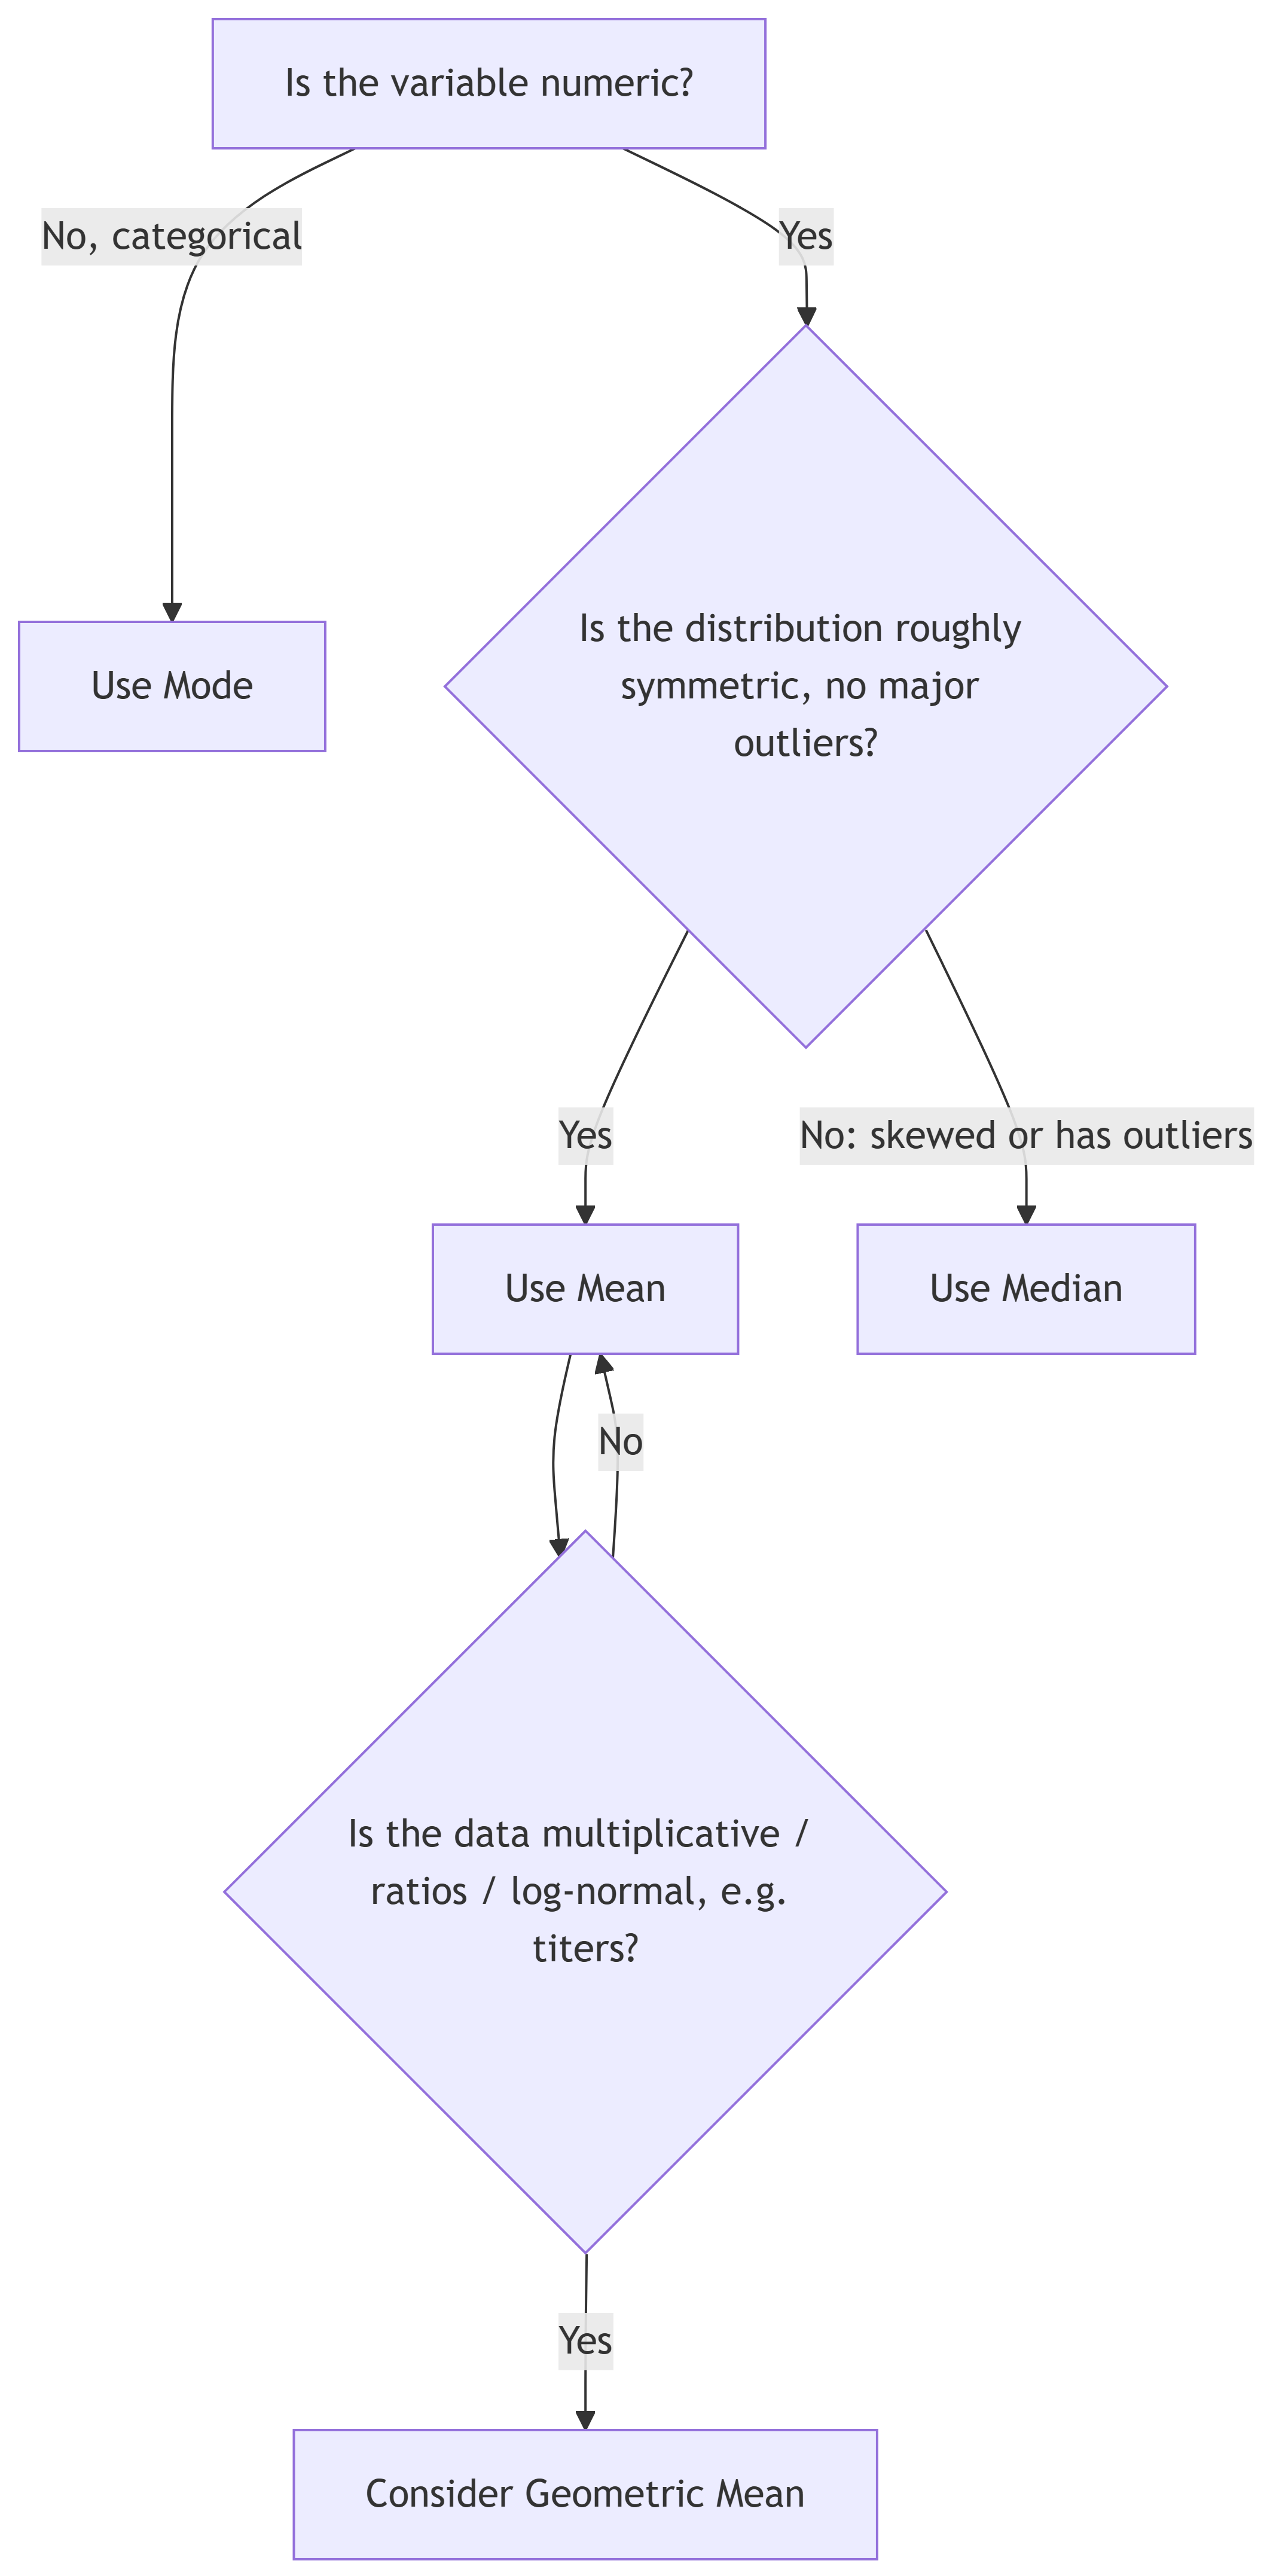
\includegraphics[width=5.54in,height=11.23in]{Section2/02_measures_central_tendency_files/figure-latex/mermaid-figure-1.png}

\textbf{Relationship between mean, median, and skewness:}

\begin{itemize}
\tightlist
\item
  \textbf{Symmetric distribution:} Mean ≈ Median ≈ Mode.
\item
  \textbf{Right-skewed (positively skewed) distribution} (e.g., income,
  hospital charges, our Data Set A with the outlier of 250): Mean
  \textgreater{} Median \textgreater{} Mode.
\item
  \textbf{Left-skewed (negatively skewed) distribution} (e.g., age at
  death from a disease mostly affecting the elderly): Mean \textless{}
  Median \textless{} Mode.
\end{itemize}

In Data Set A: Mean = 117.4, Median = 104 --- the mean exceeds the
median, correctly signaling a right-skewed distribution due to the
outlier.

\section{Summary}\label{summary-1}

\begin{itemize}
\tightlist
\item
  The \textbf{mean} is the most commonly used and mathematically useful
  measure, but it is sensitive to outliers and skewness.
\item
  The \textbf{weighted mean} correctly combines subgroup values with
  different levels of importance/sample size.
\item
  The \textbf{geometric mean} and \textbf{harmonic mean} are specialized
  means for multiplicative data and rates, respectively;
  \(HM \le GM \le AM\).
\item
  The \textbf{median} is robust to outliers and skewness and is
  preferred for skewed public health data such as income or survival
  time.
\item
  The \textbf{mode} is the only central tendency measure usable with
  nominal data.
\item
  \textbf{Quartiles, percentiles, and deciles} describe an individual's
  position within a distribution and underlie growth charts and
  reference ranges.
\end{itemize}

Section 3 builds directly on these concepts by covering \textbf{measures
of dispersion}, which quantify how spread out the data are around these
central values.

\chapter{Measures of Dispersion}\label{measures-of-dispersion}

\section{Introduction}\label{introduction-2}

A measure of central tendency alone can be misleading. Two data sets can
have the \textbf{same mean} but very different \textbf{spreads}. For
example, two clinics may both report a mean systolic blood pressure of
130 mmHg, but in Clinic A all patients cluster tightly between 125--135
mmHg, while in Clinic B patients range from 90--180 mmHg.
\textbf{Measures of dispersion (variability)} quantify this spread and
are therefore essential complements to measures of central tendency.

We continue using the same running data sets introduced in Section 2:

\begin{itemize}
\tightlist
\item
  \textbf{Data Set A (raw data):} Fasting glucose (mg/dL), \(n=11\): 88,
  92, 95, 98, 101, 104, 108, 112, 118, 125, 250.
\item
  \textbf{Data Set B (frequency table):} Number of children per
  household, \(n=40\).
\item
  \textbf{Data Set C (grouped data):} Age of 50 hypertension patients.
\end{itemize}

\section{Range}\label{range-1}

\subsection{Formula}\label{formula-5}

\[\text{Range} = \text{Maximum} - \text{Minimum}\]

\subsection{Manual Calculation --- Data Set
A}\label{manual-calculation-data-set-a}

\[\text{Range} = 250 - 88 = 162 \text{ mg/dL}\]

\subsection{Manual Calculation --- Data Set C
(Grouped)}\label{manual-calculation-data-set-c-grouped}

For grouped data, the range is estimated using the class boundaries:
upper boundary of the last class minus lower boundary of the first
class. \[\text{Range} = 89.5 - 29.5 = 60 \text{ years}\]

\subsection{Interpretation}\label{interpretation-7}

The range describes the total spread covered by the data, from smallest
to largest value.

\subsection{Applications}\label{applications}

Quick, rough check of variability; used in quality control charts (e.g.,
range charts in laboratory quality assurance) and as a preliminary check
before deeper analysis.

\subsection{Pros and Cons}\label{pros-and-cons}

\begin{longtable}[]{@{}
  >{\raggedright\arraybackslash}p{(\linewidth - 2\tabcolsep) * \real{0.5000}}
  >{\raggedright\arraybackslash}p{(\linewidth - 2\tabcolsep) * \real{0.5000}}@{}}
\toprule\noalign{}
\begin{minipage}[b]{\linewidth}\raggedright
Pros
\end{minipage} & \begin{minipage}[b]{\linewidth}\raggedright
Cons
\end{minipage} \\
\midrule\noalign{}
\endhead
\bottomrule\noalign{}
\endlastfoot
Very easy and fast to compute & Uses only 2 data points; ignores the
distribution of everything in between \\
Intuitive to understand & Extremely sensitive to outliers (a single
extreme value inflates the range) \\
& Tends to increase with sample size, making comparisons across
different \(n\) unreliable \\
\end{longtable}

\section{Interquartile Range (IQR)}\label{interquartile-range-iqr}

\subsection{Formula}\label{formula-6}

\[IQR = Q_3 - Q_1\]

The IQR represents the range of the \textbf{middle 50\%} of the data,
and is the basis for detecting outliers using \textbf{Tukey's fences}:
\[\text{Lower fence} = Q_1 - 1.5 \times IQR \qquad \text{Upper fence} = Q_3 + 1.5\times IQR\]
Any observation outside these fences is flagged as a potential outlier
(used to construct box-and-whisker plots).

\subsection{Manual Calculation --- Data Set
A}\label{manual-calculation-data-set-a-1}

From Section 2: \(Q_1 = 95\), \(Q_3 = 118\).
\[IQR = 118 - 95 = 23 \text{ mg/dL}\]

\textbf{Outlier check using Tukey's fences:}

\textbf{Step 1.} Lower fence \(= 95 - 1.5(23) = 95 - 34.5 = 60.5\).
\textbf{Step 2.} Upper fence \(= 118 + 1.5(23) = 118 + 34.5 = 152.5\).
\textbf{Step 3.} Any value below 60.5 or above 152.5 is a potential
outlier. Our value of \textbf{250} exceeds 152.5, confirming it is a
statistical outlier --- consistent with our earlier observation that it
distorted the mean.

\subsection{Manual Calculation --- Data Set C
(Grouped)}\label{manual-calculation-data-set-c-grouped-1}

From Section 2, \(Q_1 = 48.9\) years. Using the same method, \(Q_3\)
(75th percentile) is found:

\textbf{Step 1.} Position: \(\frac{3 \times 50}{4} = 37.5\).
\textbf{Step 2.} Cumulative frequencies (4, 13, 28, 41, 48, 50) show
37.5 falls in the \textbf{60--69} class (\(CF\) jumps from 28 to 41).
\textbf{Step 3.} \(L=59.5\), \(CF_{\text{before}}=28\), \(f=13\),
\(h=10\). \textbf{Step 4.}
\(Q_3 = 59.5 + \left(\frac{37.5-28}{13}\right)\times 10 = 59.5+7.31=66.8\)
years.

\[IQR = 66.8 - 48.9 = 17.9 \text{ years}\]

\subsection{Interpretation}\label{interpretation-8}

The middle 50\% of hypertension patients in Data Set C span an age range
of 17.9 years (from 48.9 to 66.8 years).

\subsection{Applications}\label{applications-1}

Constructing \textbf{box-and-whisker plots}, detecting outliers,
describing spread of skewed distributions (e.g., hospital length of
stay, cost data).

\subsection{Pros and Cons}\label{pros-and-cons-1}

\begin{longtable}[]{@{}
  >{\raggedright\arraybackslash}p{(\linewidth - 2\tabcolsep) * \real{0.5000}}
  >{\raggedright\arraybackslash}p{(\linewidth - 2\tabcolsep) * \real{0.5000}}@{}}
\toprule\noalign{}
\begin{minipage}[b]{\linewidth}\raggedright
Pros
\end{minipage} & \begin{minipage}[b]{\linewidth}\raggedright
Cons
\end{minipage} \\
\midrule\noalign{}
\endhead
\bottomrule\noalign{}
\endlastfoot
Robust to outliers (unaffected by extreme values) & Ignores the tails
(25\% smallest and 25\% largest values) entirely \\
Appropriate for skewed data & Does not use every data point \\
Basis for standard outlier detection rule & Less familiar to
non-technical audiences than the range \\
\end{longtable}

\section{Variance}\label{variance-1}

\subsection{Definition}\label{definition-6}

\textbf{Variance} measures the average squared deviation of each
observation from the mean. Squaring the deviations prevents positive and
negative deviations from canceling out and gives greater weight to
larger deviations.

\subsection{Formula}\label{formula-7}

Population variance:
\[\sigma^2 = \frac{\sum_{i=1}^{N}(X_i - \mu)^2}{N}\]

Sample variance (uses \(n-1\), \textbf{Bessel's correction}, so that
\(s^2\) is an unbiased estimator of \(\sigma^2\)):
\[s^2 = \frac{\sum_{i=1}^{n}(x_i - \bar{x})^2}{n-1}\]

For a frequency table:
\[s^2 = \frac{\sum f_i (x_i - \bar{x})^2}{\sum f_i - 1}\]

\begin{tcolorbox}[enhanced jigsaw, bottomrule=.15mm, breakable, opacityback=0, toptitle=1mm, titlerule=0mm, bottomtitle=1mm, colback=white, arc=.35mm, rightrule=.15mm, toprule=.15mm, leftrule=.75mm, title=\textcolor{quarto-callout-note-color}{\faInfo}\hspace{0.5em}{Note}, colbacktitle=quarto-callout-note-color!10!white, colframe=quarto-callout-note-color-frame, coltitle=black, left=2mm, opacitybacktitle=0.6]

We divide by \(n-1\) rather than \(n\) for a \textbf{sample} because
using the sample mean \(\bar x\) (rather than the true, unknown
population mean \(\mu\)) to compute deviations slightly underestimates
the true variance. Dividing by \(n-1\) (``degrees of freedom'') corrects
this bias.

\end{tcolorbox}

\subsection{Manual Calculation --- A. Raw
Data}\label{manual-calculation-a.-raw-data-1}

Data Set A: 88, 92, 95, 98, 101, 104, 108, 112, 118, 125, 250. We
already found \(\bar{x} = 117.4\).

\begin{longtable}[]{@{}lll@{}}
\toprule\noalign{}
\(x_i\) & \(x_i - \bar{x}\) & \((x_i - \bar{x})^2\) \\
\midrule\noalign{}
\endhead
\bottomrule\noalign{}
\endlastfoot
88 & -29.4 & 864.36 \\
92 & -25.4 & 645.16 \\
95 & -22.4 & 501.76 \\
98 & -19.4 & 376.36 \\
101 & -16.4 & 268.96 \\
104 & -13.4 & 179.56 \\
108 & -9.4 & 88.36 \\
112 & -5.4 & 29.16 \\
118 & 0.6 & 0.36 \\
125 & 7.6 & 57.76 \\
250 & 132.6 & 17,582.76 \\
\textbf{Sum} & 0.0 & \textbf{20,594.56} \\
\end{longtable}

\textbf{Step 1.} Compute \(\bar{x} = 117.4\) (from Section 2).
\textbf{Step 2.} Subtract the mean from each value (\(x_i - \bar{x}\)),
shown in column 2. Note these sum to (approximately) zero --- a useful
check. \textbf{Step 3.} Square each deviation, shown in column 3.
\textbf{Step 4.} Sum the squared deviations:
\(\sum(x_i-\bar{x})^2 = 20{,}594.56\). \textbf{Step 5.} Divide by
\(n-1 = 10\):
\[s^2 = \frac{20{,}594.56}{10} = 2059.46 \text{ (mg/dL)}^2\]

\subsection{Manual Calculation --- B. Frequency
Table}\label{manual-calculation-b.-frequency-table}

Data Set B (children per household), \(\bar{x} = 1.775\):

\begin{longtable}[]{@{}lllll@{}}
\toprule\noalign{}
\(x\) & \(f\) & \(x-\bar{x}\) & \((x-\bar{x})^2\) &
\(f(x-\bar{x})^2\) \\
\midrule\noalign{}
\endhead
\bottomrule\noalign{}
\endlastfoot
0 & 6 & -1.775 & 3.1506 & 18.9038 \\
1 & 10 & -0.775 & 0.6006 & 6.0063 \\
2 & 14 & 0.225 & 0.0506 & 0.7088 \\
3 & 7 & 1.225 & 1.5006 & 10.5044 \\
4 & 3 & 2.225 & 4.9506 & 14.8519 \\
\textbf{Total} & 40 & & & \textbf{51.0 (rounded)} \\
\end{longtable}

\textbf{Step 1--4.} Compute \(x - \bar{x}\), square it, multiply by
\(f\), then sum (shown above): \(\sum f(x-\bar{x})^2 \approx 50.98\).
\textbf{Step 5.} Divide by \(n - 1 = 39\):
\[s^2 = \frac{50.98}{39} = 1.307 \text{ children}^2\]

\subsection{Manual Calculation --- C. Grouped
Data}\label{manual-calculation-c.-grouped-data}

Data Set C, \(\bar{x} = 57.7\) years:

\begin{longtable}[]{@{}llllll@{}}
\toprule\noalign{}
Class & \(m\) & \(f\) & \(m-\bar{x}\) & \((m-\bar{x})^2\) &
\(f(m-\bar{x})^2\) \\
\midrule\noalign{}
\endhead
\bottomrule\noalign{}
\endlastfoot
30--39 & 34.5 & 4 & -23.2 & 538.24 & 2152.96 \\
40--49 & 44.5 & 9 & -13.2 & 174.24 & 1568.16 \\
50--59 & 54.5 & 15 & -3.2 & 10.24 & 153.60 \\
60--69 & 64.5 & 13 & 6.8 & 46.24 & 601.12 \\
70--79 & 74.5 & 7 & 16.8 & 282.24 & 1975.68 \\
80--89 & 84.5 & 2 & 26.8 & 718.24 & 1436.48 \\
\textbf{Total} & & 50 & & & \textbf{7888.0} \\
\end{longtable}

\textbf{Step 1--4.} Compute midpoint deviations from the mean, square
them, multiply by frequency, then sum: \(\sum f(m-\bar{x})^2 = 7888.0\).
\textbf{Step 5.} Divide by \(n-1=49\):
\[s^2 = \frac{7888.0}{49} = 160.98 \text{ years}^2\]

\subsection{Interpretation}\label{interpretation-9}

Variance is expressed in \textbf{squared units} (e.g., mg²/dL²), which
makes it difficult to interpret directly on the original measurement
scale --- this is the main motivation for the standard deviation, below.

\subsection{Applications}\label{applications-2}

Variance is the building block for standard deviation, ANOVA (analysis
of variance), regression, and virtually all inferential statistics.

\subsection{Pros and Cons}\label{pros-and-cons-2}

\begin{longtable}[]{@{}
  >{\raggedright\arraybackslash}p{(\linewidth - 2\tabcolsep) * \real{0.5000}}
  >{\raggedright\arraybackslash}p{(\linewidth - 2\tabcolsep) * \real{0.5000}}@{}}
\toprule\noalign{}
\begin{minipage}[b]{\linewidth}\raggedright
Pros
\end{minipage} & \begin{minipage}[b]{\linewidth}\raggedright
Cons
\end{minipage} \\
\midrule\noalign{}
\endhead
\bottomrule\noalign{}
\endlastfoot
Uses every observation & Expressed in squared units --- not directly
interpretable \\
Mathematically tractable, foundational for advanced methods & Very
sensitive to outliers (squaring amplifies large deviations, as seen with
250 in Data Set A) \\
\end{longtable}

\section{Standard Deviation}\label{standard-deviation-1}

\subsection{Definition}\label{definition-7}

The \textbf{standard deviation (SD)} is the square root of the variance,
returning the measure of spread to the \textbf{original units} of the
data.

\subsection{Formula}\label{formula-8}

\[s = \sqrt{s^2} = \sqrt{\frac{\sum(x_i-\bar{x})^2}{n-1}}\]

\subsection{Manual Calculation --- All Three Data
Sets}\label{manual-calculation-all-three-data-sets}

\begin{itemize}
\tightlist
\item
  \textbf{Data Set A:} \(s = \sqrt{2059.46} = 45.4\) mg/dL.
\item
  \textbf{Data Set B:} \(s = \sqrt{1.307} = 1.14\) children.
\item
  \textbf{Data Set C:} \(s = \sqrt{160.98} = 12.7\) years.
\end{itemize}

\subsection{Interpretation}\label{interpretation-10}

The SD represents the ``typical'' or ``average'' distance of an
observation from the mean. For Data Set A, a typical fasting glucose
reading is about 45.4 mg/dL away from the mean of 117.4 mg/dL (though
this is inflated by the outlier of 250). For approximately normal data,
the \textbf{empirical rule} applies: about 68\% of observations fall
within \(\bar{x} \pm 1s\), 95\% within \(\bar{x}\pm2s\), and 99.7\%
within \(\bar{x}\pm3s\).

\subsection{Applications}\label{applications-3}

SD is used to construct \textbf{reference ranges} (e.g., ``normal'' lab
values are often defined as mean ± 2 SD), calculate \textbf{z-scores},
determine \textbf{sample sizes}, and compute \textbf{confidence
intervals} (Section 11) and \textbf{effect sizes}.

\subsection{Pros and Cons}\label{pros-and-cons-3}

\begin{longtable}[]{@{}
  >{\raggedright\arraybackslash}p{(\linewidth - 2\tabcolsep) * \real{0.5000}}
  >{\raggedright\arraybackslash}p{(\linewidth - 2\tabcolsep) * \real{0.5000}}@{}}
\toprule\noalign{}
\begin{minipage}[b]{\linewidth}\raggedright
Pros
\end{minipage} & \begin{minipage}[b]{\linewidth}\raggedright
Cons
\end{minipage} \\
\midrule\noalign{}
\endhead
\bottomrule\noalign{}
\endlastfoot
Same units as original data --- directly interpretable & Sensitive to
outliers and skewness \\
Widely used, well understood, foundation of many statistical procedures
& Assumes meaningful arithmetic mean; less appropriate for skewed
data \\
\end{longtable}

\section{Mean Absolute Deviation
(MAD)}\label{mean-absolute-deviation-mad}

\subsection{Definition}\label{definition-8}

The \textbf{Mean Absolute Deviation} is the average of the
\emph{absolute} values of the deviations from the mean, avoiding the
squaring used in variance.

\subsection{Formula}\label{formula-9}

\[MAD = \frac{\sum_{i=1}^{n}|x_i - \bar{x}|}{n}\]

\subsection{Manual Calculation --- Data Set
A}\label{manual-calculation-data-set-a-2}

\begin{longtable}[]{@{}ll@{}}
\toprule\noalign{}
\(x_i\) & \(|x_i - \bar{x}|\) \\
\midrule\noalign{}
\endhead
\bottomrule\noalign{}
\endlastfoot
88 & 29.4 \\
92 & 25.4 \\
95 & 22.4 \\
98 & 19.4 \\
101 & 16.4 \\
104 & 13.4 \\
108 & 9.4 \\
112 & 5.4 \\
118 & 0.6 \\
125 & 7.6 \\
250 & 132.6 \\
\textbf{Sum} & \textbf{282.0} \\
\end{longtable}

\textbf{Step 1.} Compute the absolute deviation of each value from the
mean (117.4), shown above. \textbf{Step 2.} Sum the absolute deviations:
\(282.0\). \textbf{Step 3.} Divide by \(n = 11\):
\[MAD = \frac{282.0}{11} = 25.6 \text{ mg/dL}\]

Compare to \(s = 45.4\): because MAD does not square deviations, it is
far less inflated by the outlier of 250 than the SD is.

\subsection{Interpretation}\label{interpretation-11}

On average, an observation is 25.6 mg/dL away from the mean.

\subsection{Applications}\label{applications-4}

Used in robust statistics, forecast-error evaluation, and quality
control, especially when a measure of spread less sensitive to outliers
than SD is desired but a full rank-based measure (like IQR) is not
preferred.

\subsection{Pros and Cons}\label{pros-and-cons-4}

\begin{longtable}[]{@{}
  >{\raggedright\arraybackslash}p{(\linewidth - 2\tabcolsep) * \real{0.5000}}
  >{\raggedright\arraybackslash}p{(\linewidth - 2\tabcolsep) * \real{0.5000}}@{}}
\toprule\noalign{}
\begin{minipage}[b]{\linewidth}\raggedright
Pros
\end{minipage} & \begin{minipage}[b]{\linewidth}\raggedright
Cons
\end{minipage} \\
\midrule\noalign{}
\endhead
\bottomrule\noalign{}
\endlastfoot
Easier to interpret than variance (original units, no squaring) & Less
mathematically tractable (absolute value is not differentiable at 0), so
rarely used in advanced inferential methods \\
Less sensitive to outliers than variance/SD & Less commonly reported;
audiences less familiar with it than SD \\
\end{longtable}

\section{Coefficient of Variation
(CV)}\label{coefficient-of-variation-cv}

\subsection{Definition}\label{definition-9}

The \textbf{Coefficient of Variation} is the standard deviation
expressed as a percentage of the mean. Because it is unitless, it allows
comparison of variability \textbf{between data sets with different units
or very different means}.

\subsection{Formula}\label{formula-10}

\[CV = \frac{s}{\bar{x}} \times 100\%\]

\subsection{Manual Calculation and Worked
Comparison}\label{manual-calculation-and-worked-comparison}

Suppose we want to compare the variability of fasting glucose (Data Set
A, excluding the extreme outlier for a fairer comparison:
\(\bar x = 104.1\), \(s=11.8\)) against birth weight measurements in the
same clinic (\(\bar x = 3.2\) kg, \(s = 0.45\) kg).

\textbf{Glucose:}
\[CV_{glucose} = \frac{11.8}{104.1}\times 100\% = 11.3\%\]

\textbf{Birth weight:}
\[CV_{weight} = \frac{0.45}{3.2}\times 100\% = 14.1\%\]

\textbf{Step 1.} Compute \(s/\bar{x}\) for each variable. \textbf{Step
2.} Multiply by 100 to express as a percentage. \textbf{Step 3.}
Compare: even though glucose (mg/dL) and birth weight (kg) are on
completely different scales and units, CV allows direct comparison.
Here, birth weight (14.1\%) is relatively more variable than fasting
glucose (11.3\%) in this clinic population.

\subsection{Interpretation}\label{interpretation-12}

CV expresses variability \textbf{relative to the size of the mean}. A CV
of 11.3\% means the SD is about 11.3\% of the mean value.

\subsection{Applications}\label{applications-5}

Comparing variability of \textbf{different variables measured in
different units} (e.g., cholesterol in mg/dL vs.~BMI in kg/m²),
comparing variability of the \textbf{same variable across different
populations or time periods}, and assessing \textbf{laboratory assay
precision} (CV is a standard measure of assay reproducibility; CV
\textless{} 10-15\% is often considered acceptable).

\subsection{Pros and Cons}\label{pros-and-cons-5}

\begin{longtable}[]{@{}
  >{\raggedright\arraybackslash}p{(\linewidth - 2\tabcolsep) * \real{0.5000}}
  >{\raggedright\arraybackslash}p{(\linewidth - 2\tabcolsep) * \real{0.5000}}@{}}
\toprule\noalign{}
\begin{minipage}[b]{\linewidth}\raggedright
Pros
\end{minipage} & \begin{minipage}[b]{\linewidth}\raggedright
Cons
\end{minipage} \\
\midrule\noalign{}
\endhead
\bottomrule\noalign{}
\endlastfoot
Unitless --- enables comparison across different scales/variables &
Undefined or meaningless when the mean is zero or near zero \\
Standard tool for comparing precision of lab assays & Misleading for
data with negative values or interval-scale data without a true zero
(e.g., temperature in °C) \\
\end{longtable}

\section{Comparing SD, Variance, and
IQR}\label{comparing-sd-variance-and-iqr}

\begin{longtable}[]{@{}
  >{\raggedright\arraybackslash}p{(\linewidth - 6\tabcolsep) * \real{0.2500}}
  >{\raggedright\arraybackslash}p{(\linewidth - 6\tabcolsep) * \real{0.2500}}
  >{\raggedright\arraybackslash}p{(\linewidth - 6\tabcolsep) * \real{0.2500}}
  >{\raggedright\arraybackslash}p{(\linewidth - 6\tabcolsep) * \real{0.2500}}@{}}
\toprule\noalign{}
\begin{minipage}[b]{\linewidth}\raggedright
Feature
\end{minipage} & \begin{minipage}[b]{\linewidth}\raggedright
Variance
\end{minipage} & \begin{minipage}[b]{\linewidth}\raggedright
Standard Deviation
\end{minipage} & \begin{minipage}[b]{\linewidth}\raggedright
IQR
\end{minipage} \\
\midrule\noalign{}
\endhead
\bottomrule\noalign{}
\endlastfoot
Units & Squared original units & Original units & Original units \\
Uses all data? & Yes & Yes & No (only \(Q_1\), \(Q_3\)) \\
Robust to outliers? & No & No & \textbf{Yes} \\
Based on & Mean & Mean & Median/quantiles \\
Typical pairing & Reported alongside mean & Reported alongside mean &
Reported alongside median \\
Use case & Foundation for inferential stats (ANOVA, regression) & Most
common reported spread measure for symmetric data & Preferred spread
measure for skewed data / with box plots \\
\end{longtable}

\section{Robustness to Outliers}\label{robustness-to-outliers}

Using Data Set A (with the outlier 250) vs.~the same data with the
outlier removed (\(n=10\): 88--125):

\begin{longtable}[]{@{}
  >{\raggedright\arraybackslash}p{(\linewidth - 6\tabcolsep) * \real{0.2500}}
  >{\raggedright\arraybackslash}p{(\linewidth - 6\tabcolsep) * \real{0.2500}}
  >{\raggedright\arraybackslash}p{(\linewidth - 6\tabcolsep) * \real{0.2500}}
  >{\raggedright\arraybackslash}p{(\linewidth - 6\tabcolsep) * \real{0.2500}}@{}}
\toprule\noalign{}
\begin{minipage}[b]{\linewidth}\raggedright
Statistic
\end{minipage} & \begin{minipage}[b]{\linewidth}\raggedright
With outlier (\(n=11\))
\end{minipage} & \begin{minipage}[b]{\linewidth}\raggedright
Without outlier (\(n=10\))
\end{minipage} & \begin{minipage}[b]{\linewidth}\raggedright
\% change
\end{minipage} \\
\midrule\noalign{}
\endhead
\bottomrule\noalign{}
\endlastfoot
Mean & 117.4 & 104.1 & −11.3\% \\
Median & 104.0 & 102.5 & −1.4\% \\
SD & 45.4 & 11.8 & −74.0\% \\
IQR & 23.0 & \textasciitilde21.5 & \textasciitilde−6.5\% \\
\end{longtable}

\begin{tcolorbox}[enhanced jigsaw, bottomrule=.15mm, breakable, opacityback=0, toptitle=1mm, titlerule=0mm, bottomtitle=1mm, colback=white, arc=.35mm, rightrule=.15mm, toprule=.15mm, leftrule=.75mm, title=\textcolor{quarto-callout-important-color}{\faExclamation}\hspace{0.5em}{Important}, colbacktitle=quarto-callout-important-color!10!white, colframe=quarto-callout-important-color-frame, coltitle=black, left=2mm, opacitybacktitle=0.6]

This comparison makes the key lesson of this section concrete: removing
a single outlier changed the \textbf{mean by 11\%} and the \textbf{SD by
74\%}, but the \textbf{median} and \textbf{IQR} barely changed. When
data are skewed or contain outliers (common in public health data such
as cost, length of stay, or lab values with occasional extreme results),
the \textbf{median and IQR} should be reported as the primary summary,
often alongside the mean and SD for completeness.

\end{tcolorbox}

\section{Summary}\label{summary-2}

\begin{itemize}
\tightlist
\item
  \textbf{Range} is simple but crude --- based on only two values.
\item
  \textbf{IQR} is robust to outliers and pairs naturally with the
  median.
\item
  \textbf{Variance} and \textbf{standard deviation} use all the data and
  are mathematically central to inferential statistics, but are
  sensitive to outliers; SD is preferred for reporting because it
  retains the original units.
\item
  \textbf{MAD} is a robust, interpretable alternative to SD that is less
  commonly used in practice.
\item
  \textbf{CV} enables fair comparison of variability across variables
  with different units or scales.
\item
  When data are skewed or contain outliers, prefer \textbf{median and
  IQR}; when data are approximately symmetric, \textbf{mean and SD} are
  appropriate and more information-efficient.
\end{itemize}

Section 4 shifts from descriptive statistics to the theoretical
foundation of \textbf{probability}, which underlies all of inferential
statistics covered later in this book.

\chapter{Probability}\label{probability}

\section{Introduction}\label{introduction-3}

\textbf{Probability} is the mathematical language for quantifying
uncertainty. Everything that follows in this book --- hypothesis
testing, confidence intervals, regression, diagnostic testing --- rests
on probability theory. In biostatistics, probability lets us answer
questions such as: What is the chance that a patient with a positive
screening test truly has the disease? What is the probability that a
randomly selected newborn is preterm? How likely is it that an observed
difference between treatment groups occurred by chance alone?

\begin{tcolorbox}[enhanced jigsaw, bottomrule=.15mm, breakable, opacityback=0, toptitle=1mm, titlerule=0mm, bottomtitle=1mm, colback=white, arc=.35mm, rightrule=.15mm, toprule=.15mm, leftrule=.75mm, title=\textcolor{quarto-callout-note-color}{\faInfo}\hspace{0.5em}{Note}, colbacktitle=quarto-callout-note-color!10!white, colframe=quarto-callout-note-color-frame, coltitle=black, left=2mm, opacitybacktitle=0.6]

\textbf{Definition:} Probability is a numerical measure, between 0 and 1
(or 0\% and 100\%), of the likelihood that a particular event will
occur. A probability of 0 means the event is impossible; a probability
of 1 means the event is certain.

\end{tcolorbox}

\section{Random Experiments}\label{random-experiments}

A \textbf{random experiment} is any process or procedure that can be
repeated (at least conceptually) under the same conditions, whose
individual outcome cannot be predicted with certainty, but whose set of
\emph{possible} outcomes is known in advance.

\textbf{Examples in public health:}

\begin{itemize}
\tightlist
\item
  Testing a randomly selected patient for a disease (outcome: positive
  or negative).
\item
  Recording the number of new malaria cases in a district in one month.
\item
  Selecting a newborn and recording birth weight.
\item
  Administering a vaccine and observing whether the recipient develops
  an adverse reaction.
\end{itemize}

\section{Sample Space}\label{sample-space}

The \textbf{sample space}, denoted \(S\) or \(\Omega\), is the set of
\textbf{all possible outcomes} of a random experiment.

\textbf{Examples:}

\begin{itemize}
\tightlist
\item
  Testing a patient for a disease:
  \(S = \{\text{Positive}, \text{Negative}\}\).
\item
  Rolling a die to randomly assign a patient to 1 of 6 study arms:
  \(S=\{1,2,3,4,5,6\}\).
\item
  Recording the number of hospital-acquired infections in a month:
  \(S = \{0,1,2,3,\ldots\}\) (a countably infinite sample space).
\item
  Measuring a patient's temperature:
  \(S = (\text{all real numbers in a plausible physiological range})\),
  a continuous sample space.
\end{itemize}

\section{Events}\label{events}

An \textbf{event} is any subset of the sample space --- a collection of
one or more outcomes we are interested in. Events are typically denoted
with capital letters (\(A\), \(B\), \(C\), \ldots).

\textbf{Example:} In the die-rolling experiment for assigning patients
to 6 study arms, let \(A\) = ``patient assigned to an even-numbered
arm'' \(= \{2,4,6\}\).

\subsection{Types of Events}\label{types-of-events}

\begin{itemize}
\tightlist
\item
  \textbf{Simple (elementary) event:} Consists of exactly one outcome,
  e.g., \(\{3\}\).
\item
  \textbf{Compound event:} Consists of more than one outcome, e.g.,
  \(\{2,4,6\}\).
\item
  \textbf{Certain event:} The entire sample space \(S\); probability =
  1.
\item
  \textbf{Impossible event:} The empty set \(\emptyset\); probability =
  0.
\item
  \textbf{Complementary event (}\(A^c\) or \(\bar{A}\)): All outcomes in
  \(S\) that are \emph{not} in \(A\). \(P(A^c) = 1-P(A)\).
\item
  \textbf{Mutually exclusive (disjoint) events:} Two events that cannot
  occur at the same time, i.e., \(A \cap B = \emptyset\).
\item
  \textbf{Independent events:} The occurrence of one event does not
  affect the probability of the other.
\item
  \textbf{Dependent events:} The occurrence of one event changes the
  probability of the other.
\end{itemize}

\section{Probability Axioms (Kolmogorov's
Axioms)}\label{probability-axioms-kolmogorovs-axioms}

For any event \(A\) in sample space \(S\):

\begin{enumerate}
\def\labelenumi{\arabic{enumi}.}
\tightlist
\item
  \textbf{Non-negativity:} \(P(A) \ge 0\) for every event \(A\).
\item
  \textbf{Normalization:} \(P(S) = 1\) (something in the sample space
  must happen).
\item
  \textbf{Additivity:} For any two \textbf{mutually exclusive} events
  \(A\) and \(B\): \(P(A \cup B) = P(A) + P(B)\). (More generally, for a
  countable sequence of mutually exclusive events, the probability of
  their union is the sum of their probabilities.)
\end{enumerate}

From these three axioms, all other probability rules can be derived,
including \(P(A^c) = 1 - P(A)\) and \(0 \le P(A) \le 1\).

\section{Three Approaches to Assigning
Probability}\label{three-approaches-to-assigning-probability}

\subsection{1. Classical (A Priori)
Probability}\label{classical-a-priori-probability}

Applies when all outcomes in the sample space are \textbf{equally
likely}.
\[P(A) = \frac{\text{Number of outcomes favorable to } A}{\text{Total number of outcomes in } S}\]

\textbf{Worked example:} A study randomizes patients to one of 4 equally
likely treatment arms. The probability a given patient is assigned to
Arm 1 is \(P(\text{Arm 1}) = 1/4 = 0.25\).

\subsection{2. Empirical (Relative Frequency)
Probability}\label{empirical-relative-frequency-probability}

Based on \textbf{observed data} from repeated trials or historical
records, rather than theoretical assumptions.
\[P(A) = \frac{\text{Number of times } A \text{ occurred}}{\text{Total number of trials observed}}\]

\textbf{Worked example (clinical):} Among 500 patients who underwent a
particular surgery at a hospital last year, 15 developed a
post-operative infection. The empirical probability of infection is:
\[P(\text{infection}) = \frac{15}{500} = 0.03 = 3\%\]

This is exactly how incidence proportions/risk are calculated in
epidemiology.

\subsection{3. Subjective Probability}\label{subjective-probability}

Based on \textbf{personal judgment, experience, or belief}, used when
neither equally likely outcomes nor sufficient historical data are
available.

\textbf{Example:} A clinician estimates ``I believe there is about a
70\% chance this patient's symptoms are due to a viral rather than
bacterial infection,'' based on clinical experience rather than a formal
calculation. Subjective probability underlies \textbf{prior
probabilities} in Bayesian analysis (Sections 5--6).

\section{Venn Diagrams}\label{venn-diagrams}

Venn diagrams visually represent relationships between events (sets)
within a sample space. Below, regions are labeled to show set
relationships; overlapping regions represent intersections.

\subsection{General Two-Event Venn
Diagram}\label{general-two-event-venn-diagram}

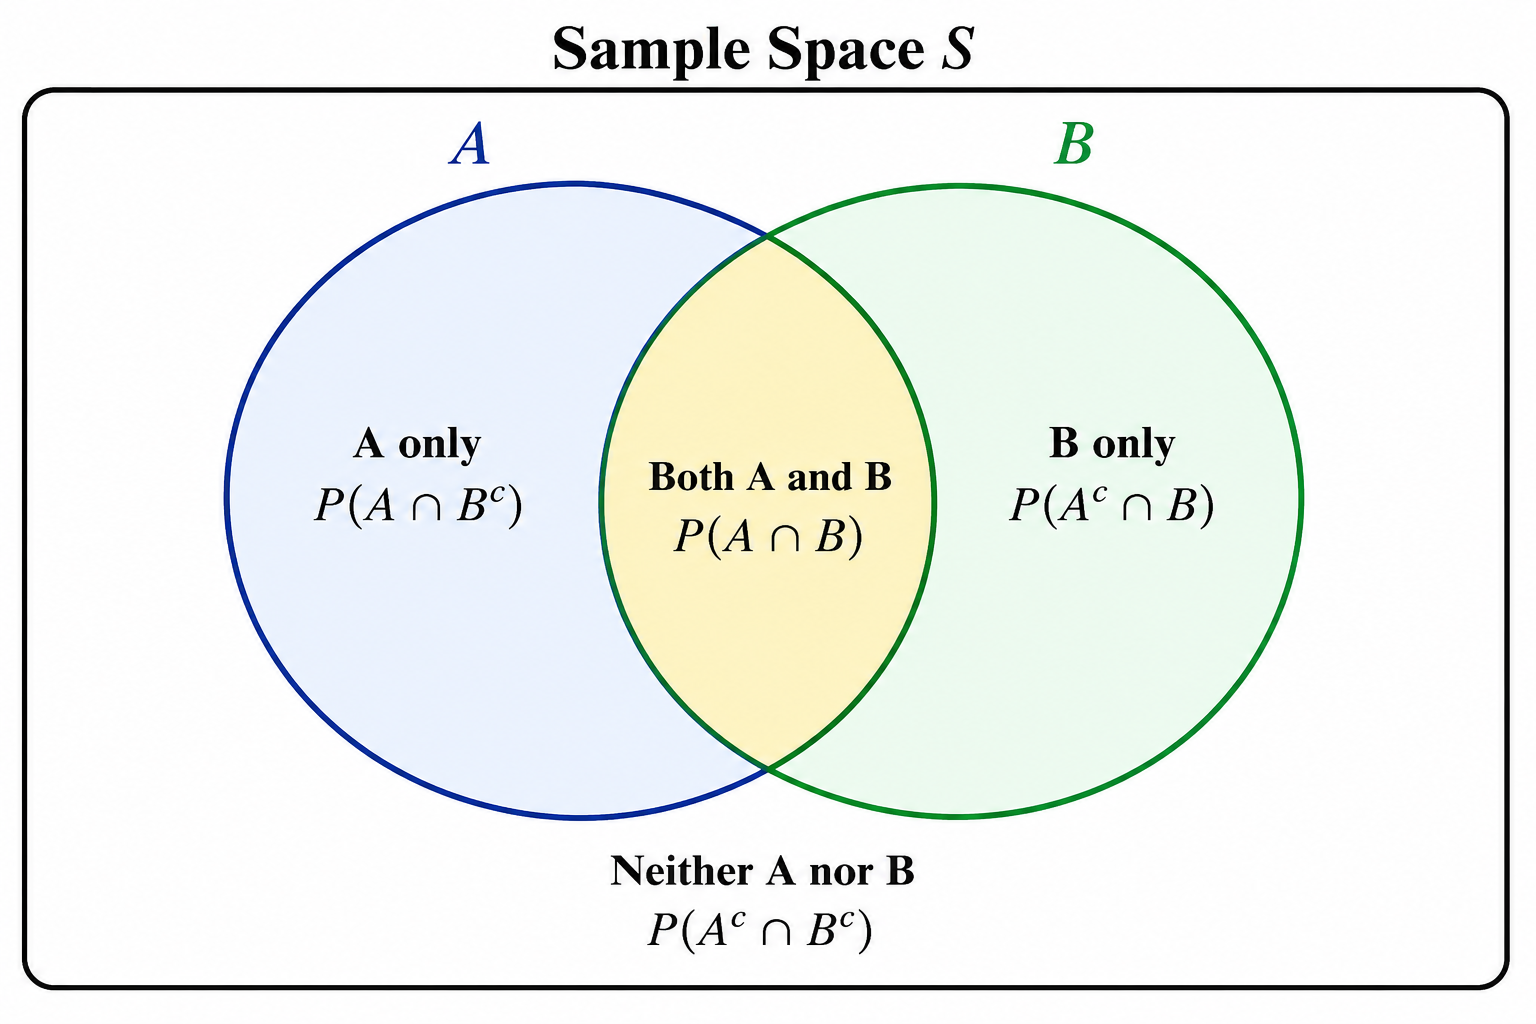
\includegraphics[width=5.22917in,height=\textheight,keepaspectratio]{Section2/images/7f2f6957-e099-4d7a-af82-90f5eae0a750.png}

\subsection{Mutually Exclusive Events (No
Overlap)}\label{mutually-exclusive-events-no-overlap}

\pandocbounded{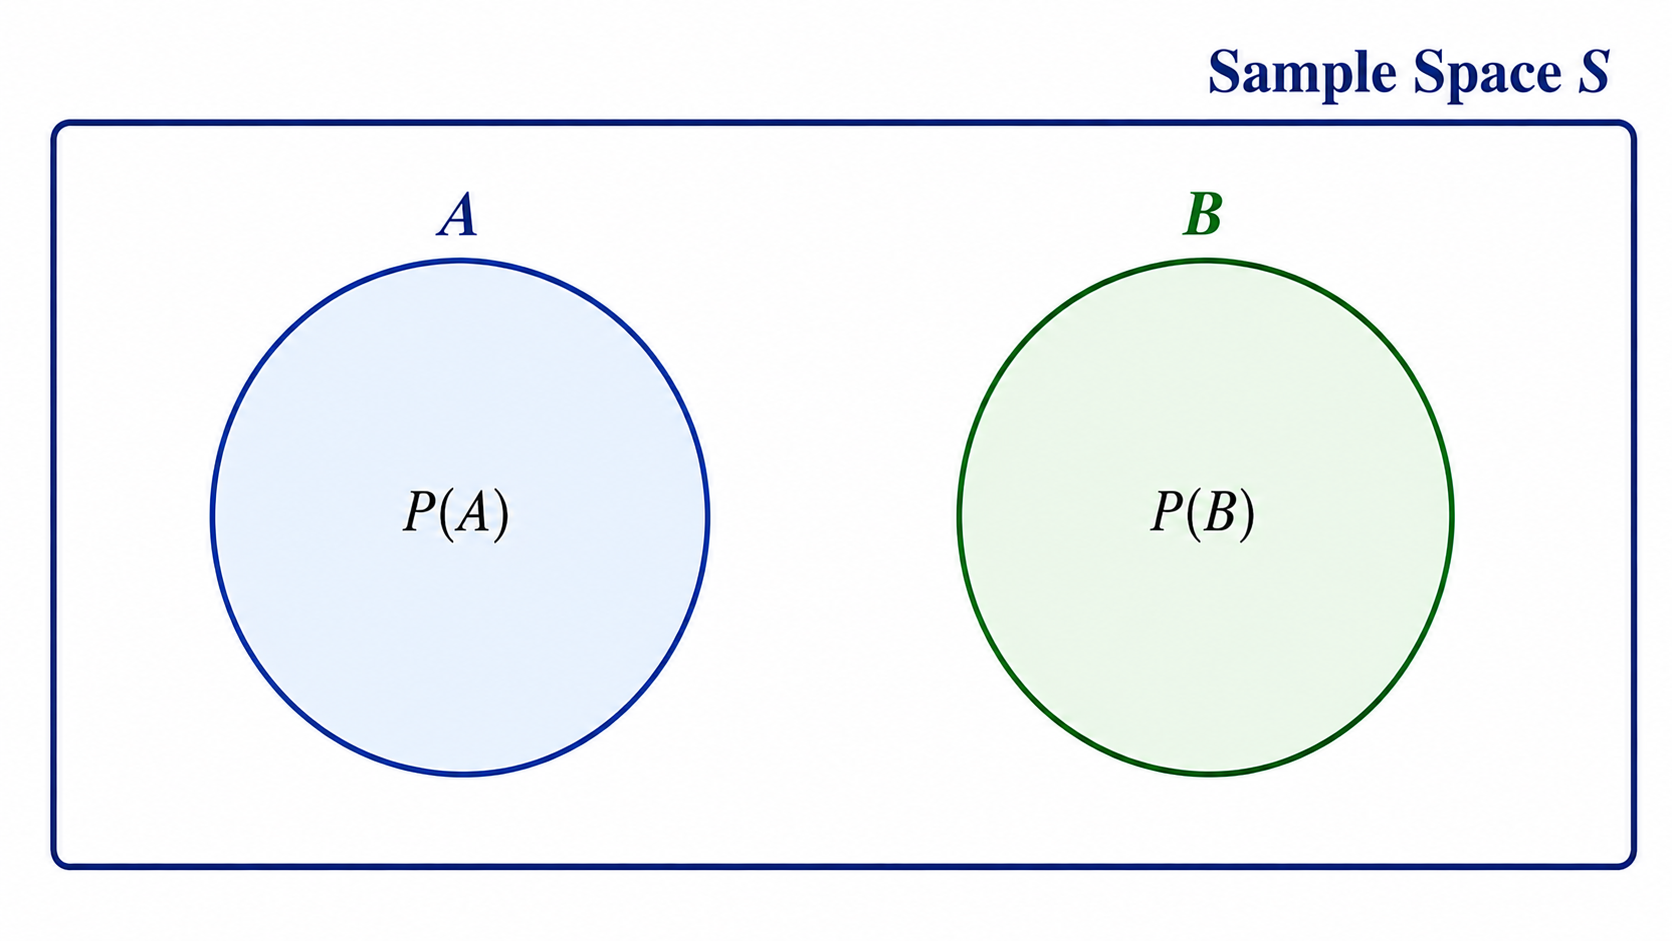
\includegraphics[keepaspectratio]{Section2/images/21eb2b12-30c4-4987-ae8b-628e810dbbb8-02.png}}

Because \(A\) and \(B\) share no outcomes, there is no overlapping
region --- this is the defining feature of mutually exclusive events.

\subsection{Clinical Example Venn
Diagram}\label{clinical-example-venn-diagram}

Let \(A\) = ``patient has diabetes'' and \(B\) = ``patient has
hypertension'' in a clinic population of 200 patients: 60 have diabetes
only, 50 have hypertension only, 40 have both, and 50 have neither.

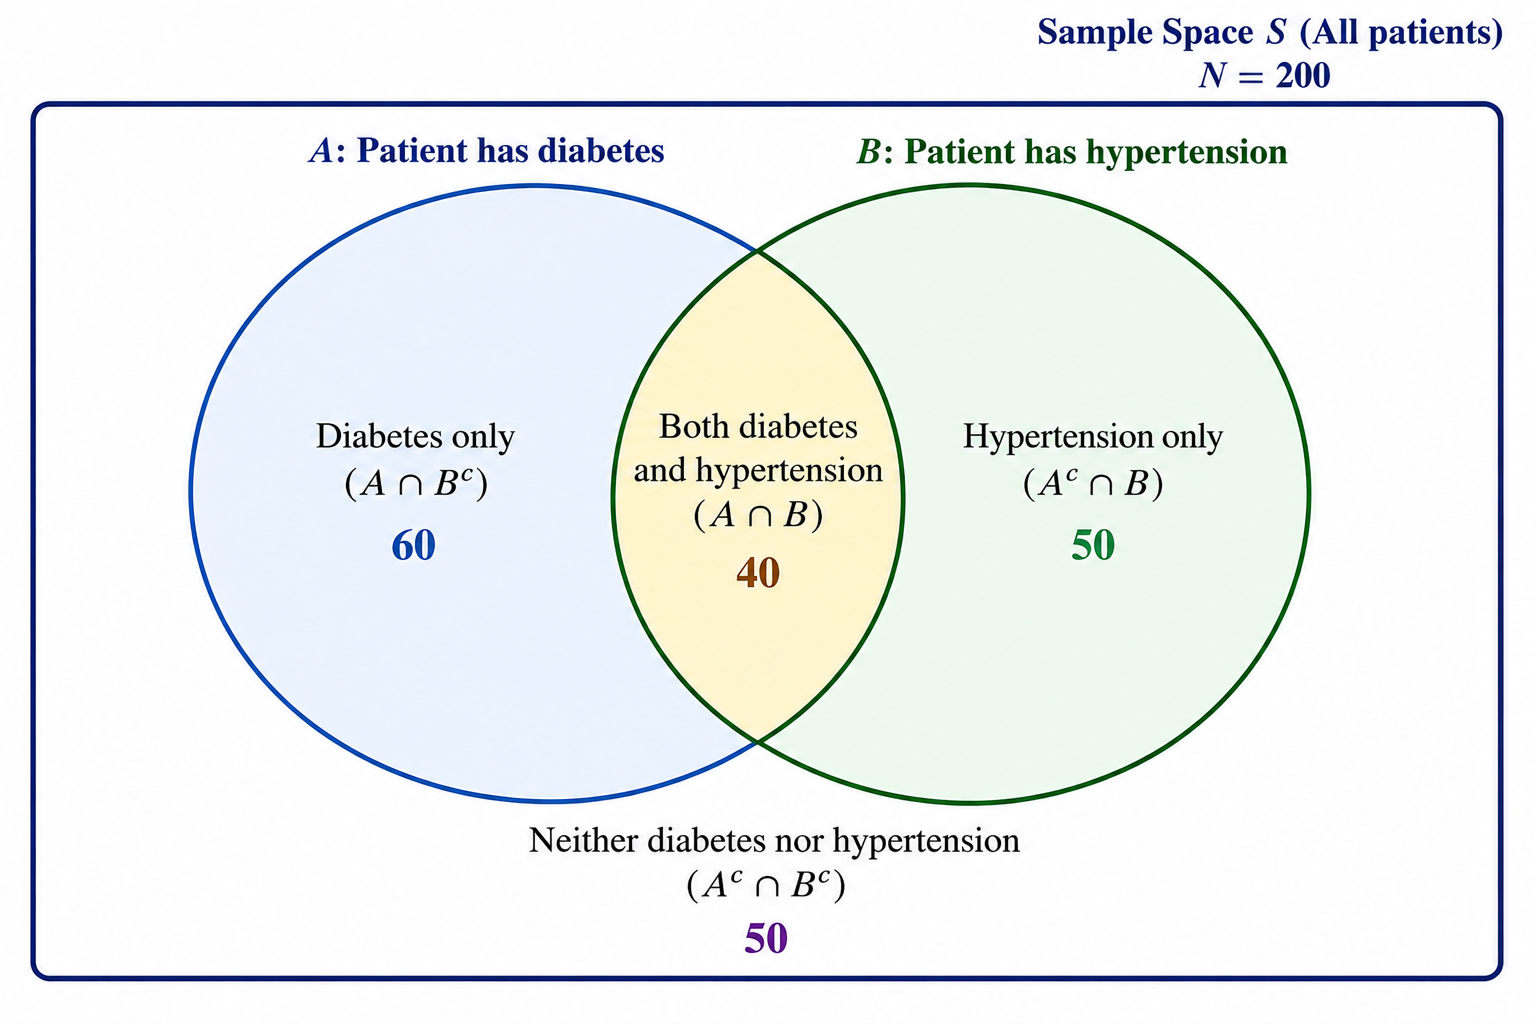
\includegraphics[width=6.8125in,height=\textheight,keepaspectratio]{Section2/images/b21f6b39-cfca-428f-88a9-8e717cadce66.png}

From this diagram:

\(P(\text{diabetes}) = (60+40)/200 = 0.50\);

\(P(\text{hypertension}) = (50+40)/200=0.45\);

\(P(\text{both}) = 40/200 = 0.20\); \(P(\text{neither}) = 50/200=0.25\).

\section{The Addition Rule}\label{the-addition-rule}

\subsection{General Addition Rule}\label{general-addition-rule}

\[P(A \cup B) = P(A) + P(B) - P(A \cap B)\]

We subtract \(P(A \cap B)\) to avoid double-counting outcomes that
belong to both events.

\subsection{Addition Rule for Mutually Exclusive
Events}\label{addition-rule-for-mutually-exclusive-events}

If \(A\) and \(B\) are mutually exclusive (\(P(A \cap B) = 0\)):
\[P(A \cup B) = P(A) + P(B)\]

\subsection{Worked Example}\label{worked-example}

Using the clinic data above (\(n=200\)): What is the probability a
randomly selected patient has diabetes \textbf{or} hypertension (or
both)?

\textbf{Step 1.} \(P(A) = P(\text{diabetes}) = 100/200 = 0.50\) (60
diabetes-only + 40 both).

\textbf{Step 2.} \(P(B) = P(\text{hypertension}) = 90/200 = 0.45\) (50
hypertension-only + 40 both).

\textbf{Step 3.} \(P(A \cap B) = 40/200 = 0.20\).

\textbf{Step 4.} Apply the addition rule:
\[P(A \cup B) = 0.50+0.45-0.20 = 0.75\]

\textbf{Verification by direct count:}
\((60+50+40)/200 = 150/200 = 0.75\) ✓. This confirms 75\% of patients
have at least one of the two conditions.

\section{Mutually Exclusive Events}\label{mutually-exclusive-events}

Two events \(A\) and \(B\) are \textbf{mutually exclusive (disjoint)} if
they cannot both occur simultaneously: \(P(A \cap B) = 0\).

\textbf{Clinical example:} A patient's ABO blood type result is a single
test outcome --- a patient cannot simultaneously be ``type A'' and
``type B'' (ignoring rare chimerism); these are mutually exclusive
events.

\section{Independent vs.~Dependent
Events}\label{independent-vs.-dependent-events}

\subsection{Independent Events}\label{independent-events}

Two events are \textbf{independent} if the occurrence of one does not
change the probability of the other:
\[P(A \cap B) = P(A) \times P(B) \quad \text{(Multiplication Rule for independent events)}\]
Equivalently, \(A\) and \(B\) are independent if \(P(A|B) = P(A)\).

\textbf{Worked example:} The sex of a first-born child and the sex of a
second-born child (in the absence of any biological linkage) are
independent. If \(P(\text{boy}) = 0.5\) for each birth, then:
\[P(\text{both children are boys}) = 0.5 \times 0.5 = 0.25\]

\subsection{Dependent Events}\label{dependent-events}

Two events are \textbf{dependent} if the occurrence of one \textbf{does}
affect the probability of the other. In this case, we must use
\textbf{conditional probability}:
\[P(A \cap B) = P(A) \times P(B|A) \quad \text{(General/Multiplication Rule)}\]

\textbf{Clinical example:} Smoking status and lung cancer diagnosis are
dependent events --- knowing a patient smokes changes the probability
that they will be diagnosed with lung cancer.

\section{Conditional Probability}\label{conditional-probability}

\subsection{Definition}\label{definition-10}

\textbf{Conditional probability} is the probability that event \(B\)
occurs, \emph{given that} event \(A\) has already occurred (or is known
to be true).

\subsection{Formula}\label{formula-11}

\[P(B|A) = \frac{P(A \cap B)}{P(A)}, \quad \text{provided } P(A) > 0\]

\subsection{Worked Example (Clinical)}\label{worked-example-clinical}

Using the clinic data (\(n=200\): 60 diabetes only, 50 hypertension
only, 40 both, 50 neither): What is the probability a patient has
hypertension, \textbf{given} that they have diabetes?

\textbf{Step 1.} \(P(\text{diabetes}) = 100/200 = 0.50\). \textbf{Step
2.} \(P(\text{diabetes} \cap \text{hypertension}) = 40/200 = 0.20\).
\textbf{Step 3.} Apply the formula:
\[P(\text{hypertension}|\text{diabetes}) = \frac{0.20}{0.50} = 0.40\]

\textbf{Interpretation:} Among diabetic patients, 40\% also have
hypertension --- noticeably higher than the overall prevalence of
hypertension in the whole clinic (45\%\ldots{} actually let's compare
correctly: overall \(P(\text{hypertension})=0.45\)). Here conditioning
on diabetes gives 40\%, close to but not equal to the unconditional
45\%, illustrating how conditioning can shift a probability up, down, or
leave it nearly unchanged depending on the strength of association
between the two conditions.

\section{The Multiplication Rule}\label{the-multiplication-rule}

\subsection{General Rule (Dependent
Events)}\label{general-rule-dependent-events}

\[P(A \cap B) = P(A)\times P(B|A)\]

\subsection{Special Case (Independent
Events)}\label{special-case-independent-events}

\[P(A \cap B) = P(A) \times P(B)\]

\subsection{Worked Example: Sequential (Dependent)
Sampling}\label{worked-example-sequential-dependent-sampling}

A batch of 10 vaccine vials contains 2 defective vials. Two vials are
selected \textbf{without replacement} for quality testing. What is the
probability both are defective?

\textbf{Step 1.} \(P(\text{1st defective}) = 2/10 = 0.20\).

\textbf{Step 2.} Given the 1st is defective, 1 defective vial remains
out of 9:
\(P(\text{2nd defective}|\text{1st defective}) = 1/9 = 0.111\).

\textbf{Step 3.} Apply the multiplication rule:
\[P(\text{both defective}) = 0.20 \times 0.111 = 0.0222 \approx 2.2\%\]

\section{Tree Diagrams}\label{tree-diagrams}

Tree diagrams visually organize sequential/conditional probabilities and
are especially useful for multi-stage experiments (they will be used
again for diagnostic testing in Section 5).

\begin{Shaded}
\begin{Highlighting}[]
\NormalTok{flowchart LR}
\NormalTok{    Start(("Select\textless{}br/\textgreater{}Vial 1")) {-}{-}\textgreater{}|"P = 0.20\textless{}br/\textgreater{}Defective"| D1["1st Defective"]}
\NormalTok{    Start {-}{-}\textgreater{}|"P = 0.80\textless{}br/\textgreater{}Not Defective"| ND1["1st OK"]}
\NormalTok{    D1 {-}{-}\textgreater{}|"P = 1/9\textless{}br/\textgreater{}Defective"| D1D2["Both Defective\textless{}br/\textgreater{}P = 0.20 × 0.111 = 0.022"]}
\NormalTok{    D1 {-}{-}\textgreater{}|"P = 8/9\textless{}br/\textgreater{}Not Defective"| D1ND2["1st Def, 2nd OK\textless{}br/\textgreater{}P = 0.20 × 0.889 = 0.178"]}
\NormalTok{    ND1 {-}{-}\textgreater{}|"P = 2/9\textless{}br/\textgreater{}Defective"| ND1D2["1st OK, 2nd Def\textless{}br/\textgreater{}P = 0.80 × 0.222 = 0.178"]}
\NormalTok{    ND1 {-}{-}\textgreater{}|"P = 7/9\textless{}br/\textgreater{}Not Defective"| ND1ND2["Neither Defective\textless{}br/\textgreater{}P = 0.80 × 0.778 = 0.622"]}
\end{Highlighting}
\end{Shaded}

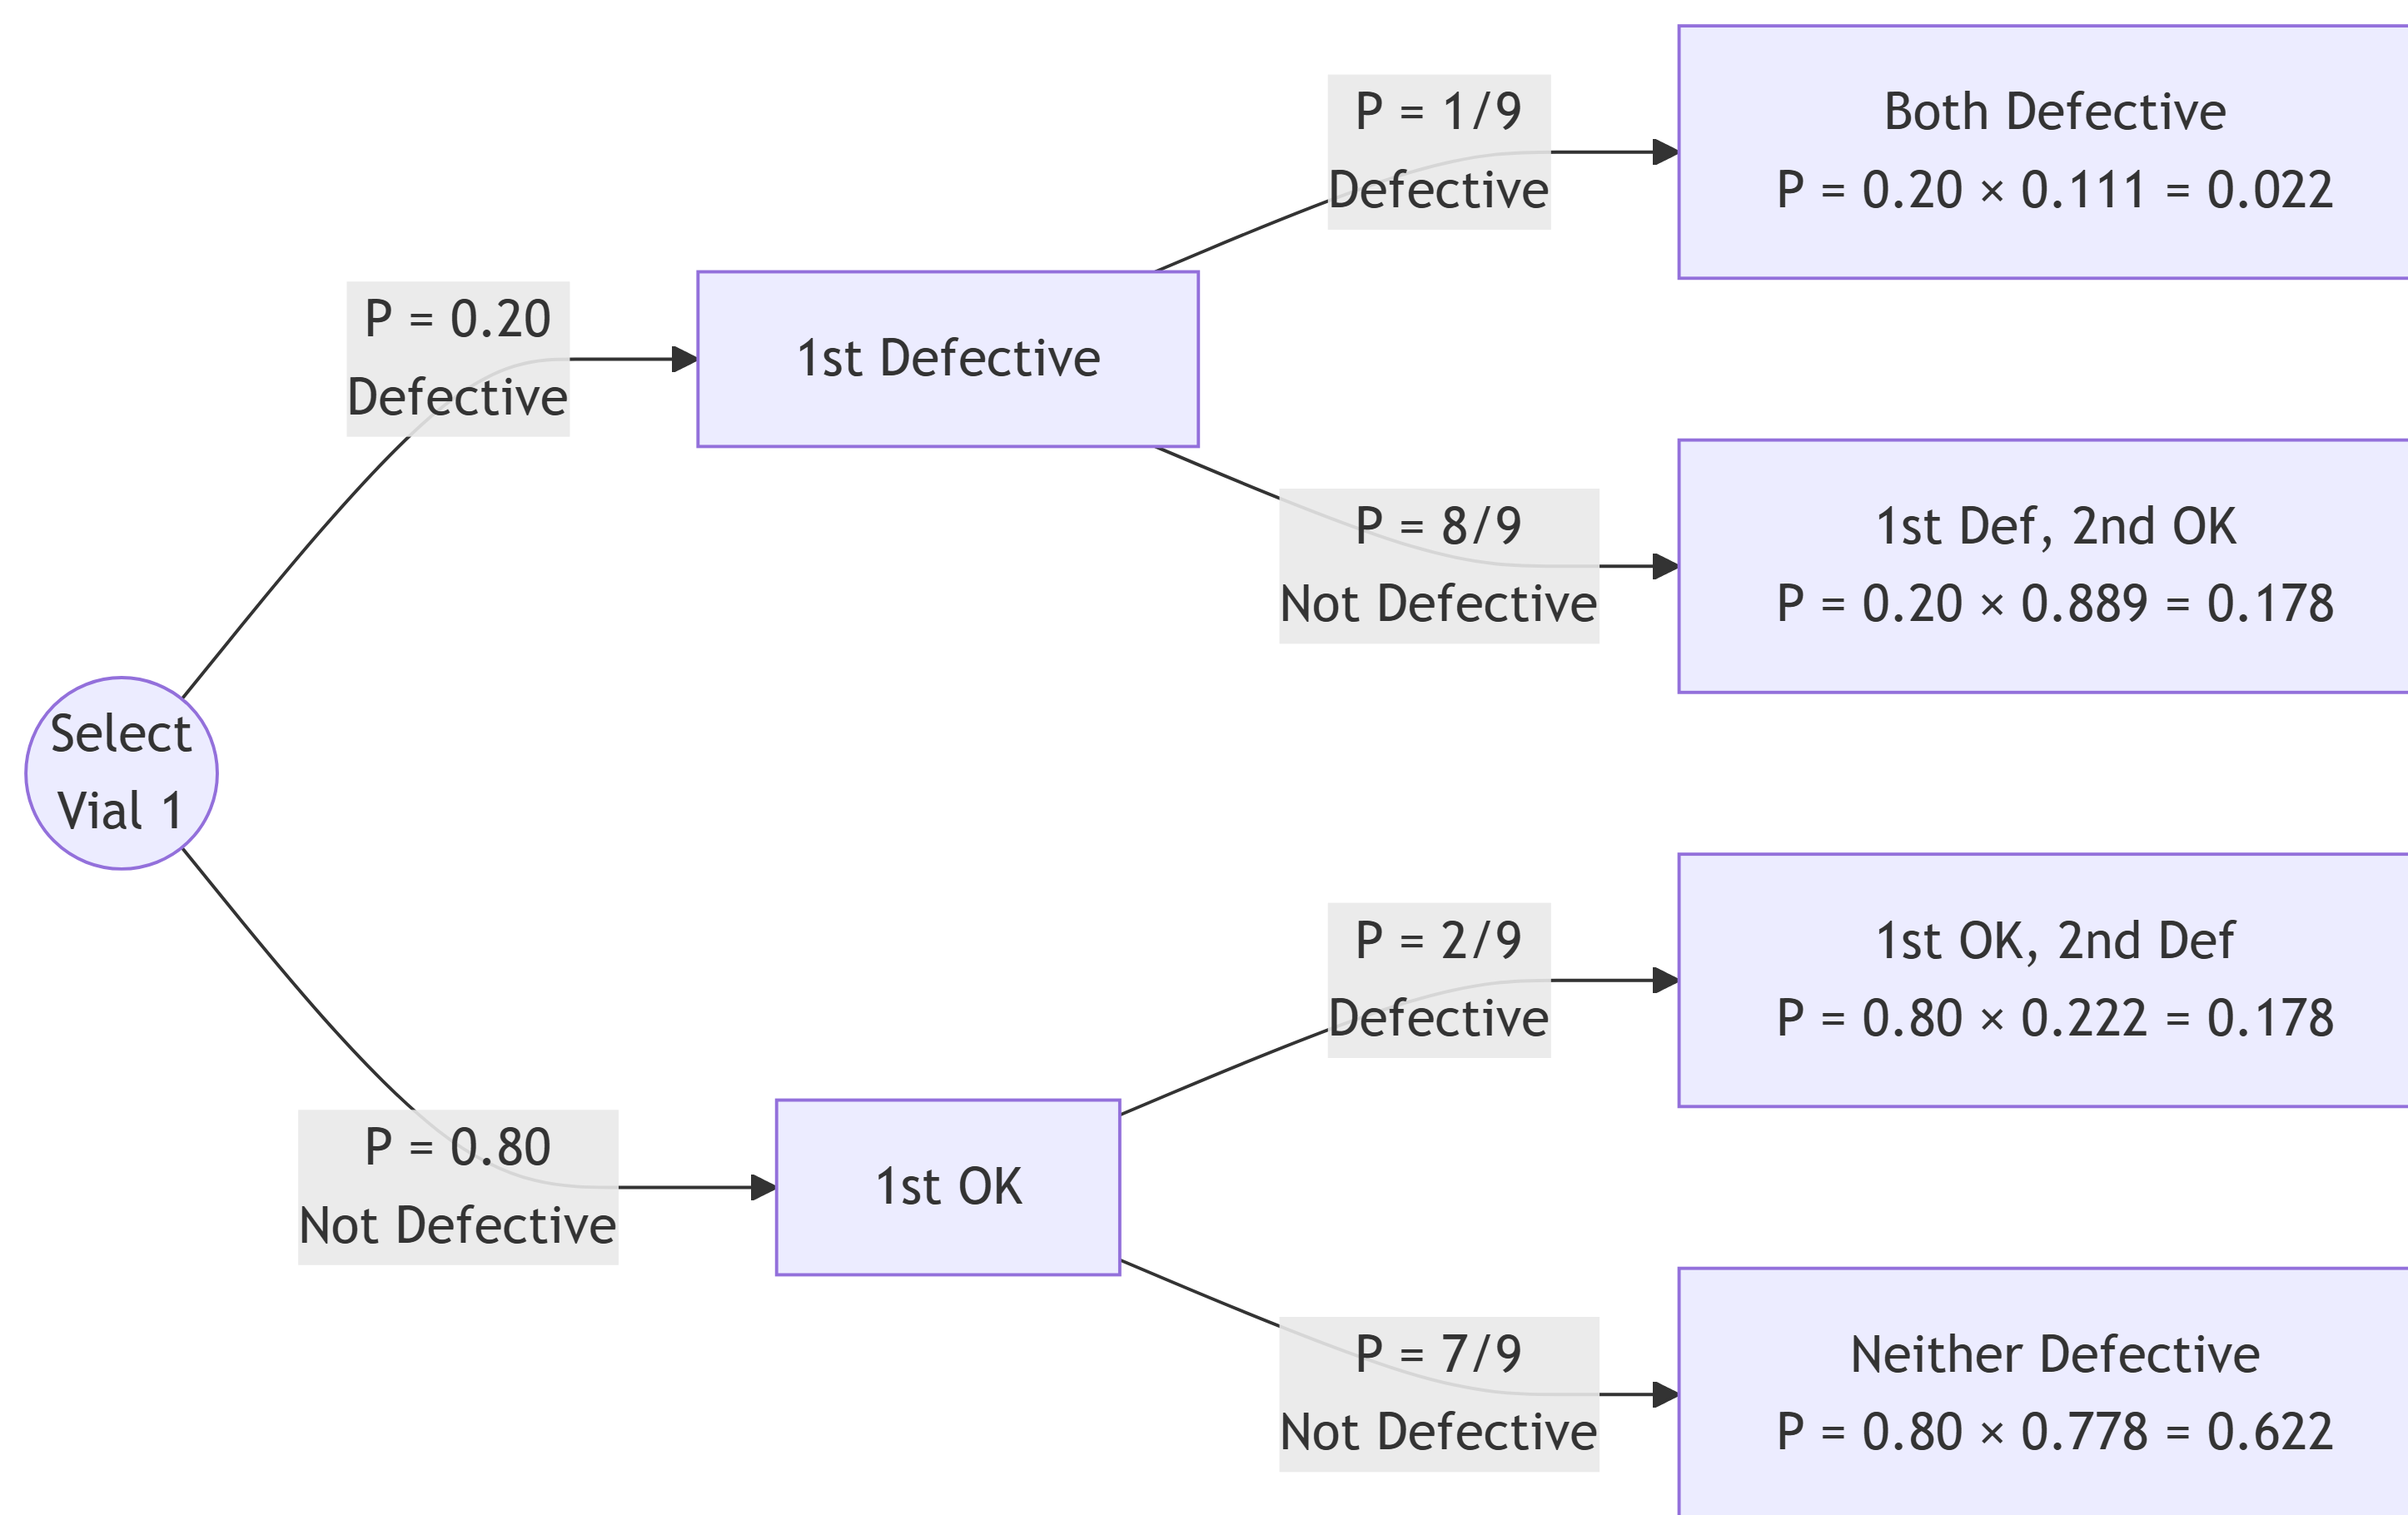
\includegraphics[width=7.91in,height=4.98in]{Section2/04_probability_files/figure-latex/mermaid-figure-1.png}

\textbf{Check:} The four end-branch probabilities should sum to 1:
\(0.022+0.178+0.178+0.622 = 1.000\) ✓.

\section{Worked Example Combining Multiple Rules
(Clinical)}\label{worked-example-combining-multiple-rules-clinical}

In a population, 10\% of people have a certain risk gene (\(G\)). Among
those with the gene, 40\% develop the disease (\(D\)) by age 60; among
those without the gene, only 5\% develop the disease. Find the overall
probability a randomly selected person develops the disease (this
previews the \textbf{Law of Total Probability}, essential for Bayes'
Theorem in Section 5).

\begin{Shaded}
\begin{Highlighting}[]
\NormalTok{flowchart LR}
\NormalTok{    Start(("Population")) {-}{-}\textgreater{}|"P(G) = 0.10"| G["Has Gene"]}
\NormalTok{    Start {-}{-}\textgreater{}|"P(Gᶜ) = 0.90"| Gc["No Gene"]}
\NormalTok{    G {-}{-}\textgreater{}|"P(D|G) = 0.40"| GD["Gene \& Disease\textless{}br/\textgreater{}P = 0.10×0.40 = 0.04"]}
\NormalTok{    G {-}{-}\textgreater{}|"P(Dᶜ|G) = 0.60"| GDc["Gene, No Disease\textless{}br/\textgreater{}P = 0.10×0.60 = 0.06"]}
\NormalTok{    Gc {-}{-}\textgreater{}|"P(D|Gᶜ) = 0.05"| GcD["No Gene, Disease\textless{}br/\textgreater{}P = 0.90×0.05 = 0.045"]}
\NormalTok{    Gc {-}{-}\textgreater{}|"P(Dᶜ|Gᶜ) = 0.95"| GcDc["No Gene, No Disease\textless{}br/\textgreater{}P = 0.90×0.95 = 0.855"]}
\end{Highlighting}
\end{Shaded}

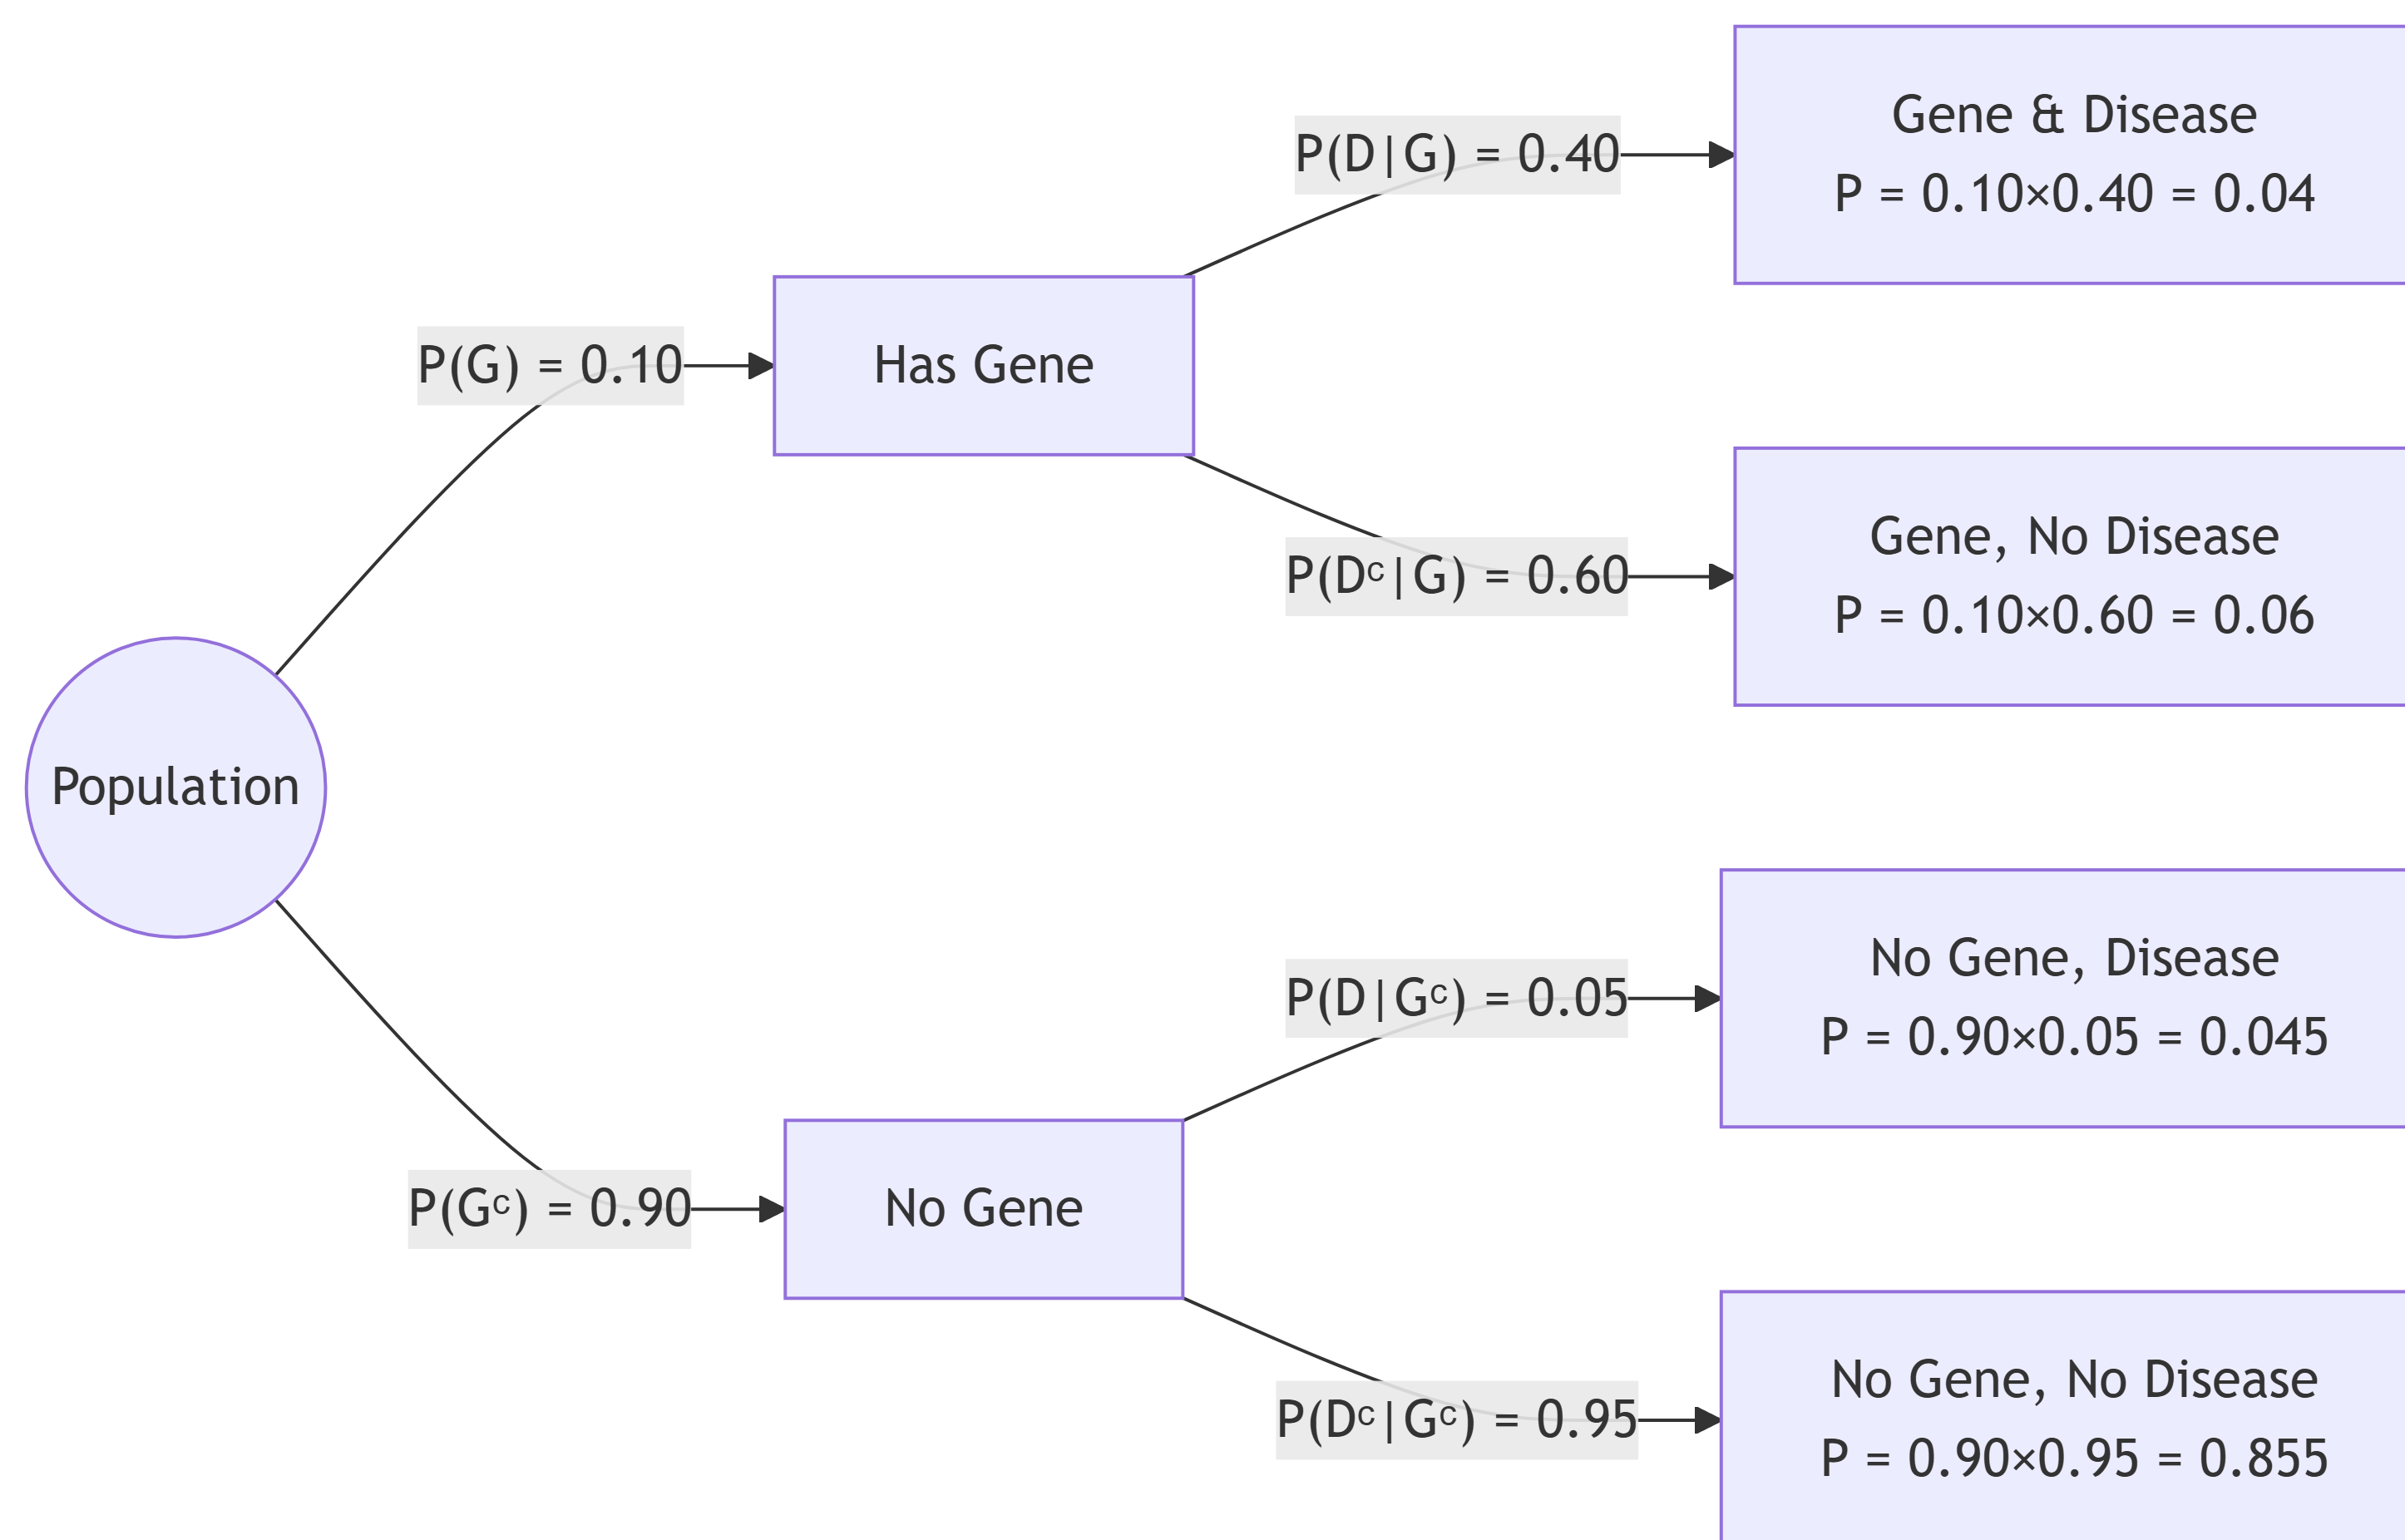
\includegraphics[width=7.76in,height=4.98in]{Section2/04_probability_files/figure-latex/mermaid-figure-3.png}

\textbf{Step 1.} Multiply along each branch (multiplication rule for
dependent events): \(P(G \cap D) = 0.04\), \(P(G^c \cap D) = 0.045\).
\textbf{Step 2.} Since ``has gene'' and ``no gene'' are mutually
exclusive and exhaustive, add the two paths that end in disease
(addition rule):
\[P(D) = P(G\cap D) + P(G^c \cap D) = 0.04+0.045 = 0.085 = 8.5\%\]

This is the \textbf{Law of Total Probability}:
\(P(D) = P(D|G)P(G) + P(D|G^c)P(G^c)\).

\chapter{Bayes' Theorem}\label{bayes-theorem}

\section{Conditional Probability
Review}\label{conditional-probability-review}

Recall from Section 4 that conditional probability is defined as:
\[P(B|A) = \frac{P(A\cap B)}{P(A)}\]

By symmetry, we can also write:
\[P(A|B) = \frac{P(A\cap B)}{P(B)} \implies P(A\cap B) = P(A|B)\,P(B)\]

Setting the two expressions for \(P(A \cap B)\) equal to each other
gives us the foundation for Bayes' Theorem:
\[P(B|A)\,P(A) = P(A|B)\,P(B)\]

\section{Bayes' Rule - Derivation}\label{bayes-rule---derivation}

Starting from \(P(B|A)\,P(A) = P(A|B)\,P(B)\), divide both sides by
\(P(A)\):

\[P(B|A) = \frac{P(A|B)\,P(B)}{P(A)}\]

This is \textbf{Bayes' Theorem}. In words: it lets us ``reverse'' a
conditional probability --- converting \(P(A|B)\) (which we may know)
into \(P(B|A)\) (which we actually want to know).

If \(P(A)\) is not known directly, it can be expanded using the
\textbf{Law of Total Probability} (introduced in Section 4), assuming
\(B\) and \(B^c\) partition the sample space:
\[P(A) = P(A|B)\,P(B) + P(A|B^c)\,P(B^c)\]

giving the most commonly used form of Bayes' Theorem:

\[\boxed{P(B|A) = \frac{P(A|B)\,P(B)}{P(A|B)\,P(B) + P(A|B^c)\,P(B^c)}}\]

\subsection{Interpretation}\label{interpretation-13}

Bayes' Theorem updates our belief about event \(B\) (e.g., ``patient has
disease'') after observing evidence \(A\) (e.g., ``test result is
positive''), by combining:

\begin{itemize}
\tightlist
\item
  \(P(B)\) : the \textbf{prior probability} of \(B\) (what we believed
  before seeing the evidence),
\item
  \(P(A|B)\) : the \textbf{likelihood} of observing the evidence if
  \(B\) is true,
\end{itemize}

to produce \(P(B|A)\) --- the \textbf{posterior probability} of \(B\)
after seeing the evidence. This prior/likelihood/posterior framework is
developed further in Section 6.

\section{Applications: Medical Diagnosis and Screening
Tests}\label{applications-medical-diagnosis-and-screening-tests}

Bayes' Theorem is the mathematical backbone of \textbf{diagnostic
testing} in medicine and \textbf{screening program evaluation} in public
health. It answers the clinically crucial question: \emph{``Given that
this patient tested positive, what is the probability they actually have
the disease?''} --- which is generally \textbf{not} the same as the
test's sensitivity.

\subsection{The Confusion Matrix}\label{the-confusion-matrix}

Diagnostic test performance is organized in a \textbf{2×2 confusion
matrix (contingency table)}, cross-classifying the true disease status
against the test result:

\begin{longtable}[]{@{}
  >{\raggedright\arraybackslash}p{(\linewidth - 6\tabcolsep) * \real{0.3158}}
  >{\raggedright\arraybackslash}p{(\linewidth - 6\tabcolsep) * \real{0.2895}}
  >{\raggedright\arraybackslash}p{(\linewidth - 6\tabcolsep) * \real{0.2763}}
  >{\raggedright\arraybackslash}p{(\linewidth - 6\tabcolsep) * \real{0.1184}}@{}}
\toprule\noalign{}
\begin{minipage}[b]{\linewidth}\raggedright
\end{minipage} & \begin{minipage}[b]{\linewidth}\raggedright
Disease Present (D+)
\end{minipage} & \begin{minipage}[b]{\linewidth}\raggedright
Disease Absent (D−)
\end{minipage} & \begin{minipage}[b]{\linewidth}\raggedright
Total
\end{minipage} \\
\midrule\noalign{}
\endhead
\bottomrule\noalign{}
\endlastfoot
\textbf{Test Positive (T+)} & True Positive (TP) & False Positive (FP) &
TP + FP \\
\textbf{Test Negative (T−)} & False Negative (FN) & True Negative (TN) &
FN + TN \\
\textbf{Total} & TP + FN & FP + TN & \(N\) \\
\end{longtable}

\begin{itemize}
\tightlist
\item
  \textbf{False positive:} Test says positive, but the patient does not
  actually have the disease (a ``false alarm'').
\item
  \textbf{False negative:} Test says negative, but the patient actually
  has the disease (a ``missed case'').
\end{itemize}

\subsection{Key Diagnostic Test
Measures}\label{key-diagnostic-test-measures}

\begin{longtable}[]{@{}
  >{\raggedright\arraybackslash}p{(\linewidth - 4\tabcolsep) * \real{0.3333}}
  >{\raggedright\arraybackslash}p{(\linewidth - 4\tabcolsep) * \real{0.3333}}
  >{\raggedright\arraybackslash}p{(\linewidth - 4\tabcolsep) * \real{0.3333}}@{}}
\toprule\noalign{}
\begin{minipage}[b]{\linewidth}\raggedright
Measure
\end{minipage} & \begin{minipage}[b]{\linewidth}\raggedright
Formula
\end{minipage} & \begin{minipage}[b]{\linewidth}\raggedright
Meaning
\end{minipage} \\
\midrule\noalign{}
\endhead
\bottomrule\noalign{}
\endlastfoot
\textbf{Sensitivity} (True Positive Rate) & \(\dfrac{TP}{TP+FN}\) &
Among those \textbf{with} disease, proportion correctly identified as
positive \\
\textbf{Specificity} (True Negative Rate) & \(\dfrac{TN}{TN+FP}\) &
Among those \textbf{without} disease, proportion correctly identified as
negative \\
\textbf{Positive Predictive Value (PPV)} & \(\dfrac{TP}{TP+FP}\) & Among
those who \textbf{test positive}, proportion who truly have disease \\
\textbf{Negative Predictive Value (NPV)} & \(\dfrac{TN}{TN+FN}\) & Among
those who \textbf{test negative}, proportion who truly do not have
disease \\
\textbf{Prevalence} & \(\dfrac{TP+FN}{N}\) & Proportion of the
population with disease \\
\textbf{Positive Likelihood Ratio (LR+)} &
\(\dfrac{\text{Sensitivity}}{1-\text{Specificity}}\) & How much a
positive result increases the odds of disease \\
\textbf{Negative Likelihood Ratio (LR−)} &
\(\dfrac{1-\text{Sensitivity}}{\text{Specificity}}\) & How much a
negative result decreases the odds of disease \\
\end{longtable}

\begin{tcolorbox}[enhanced jigsaw, bottomrule=.15mm, breakable, opacityback=0, toptitle=1mm, titlerule=0mm, bottomtitle=1mm, colback=white, arc=.35mm, rightrule=.15mm, toprule=.15mm, leftrule=.75mm, title=\textcolor{quarto-callout-important-color}{\faExclamation}\hspace{0.5em}{Important}, colbacktitle=quarto-callout-important-color!10!white, colframe=quarto-callout-important-color-frame, coltitle=black, left=2mm, opacitybacktitle=0.6]

\textbf{Sensitivity and specificity are intrinsic properties of the
test} and do not depend on disease prevalence. \textbf{PPV and NPV,
however, depend heavily on prevalence} --- the same test performs very
differently (in terms of PPV) in a high-prevalence population (e.g., a
specialist referral clinic) versus a low-prevalence population (e.g.,
mass community screening). This is precisely why Bayes' Theorem is
required to move from sensitivity/specificity to PPV/NPV.

\end{tcolorbox}

\section{Worked Example: Full Manual
Calculation}\label{worked-example-full-manual-calculation}

A tuberculosis (TB) screening test has \textbf{sensitivity = 90\%} and
\textbf{specificity = 95\%}. It is used to screen a population where the
true \textbf{prevalence of TB is 1\%}. Suppose we screen
\(N = 10{,}000\) people. Find the PPV and NPV, and interpret using
Bayes' Theorem.

\textbf{Step 1: Determine the number with and without disease using
prevalence:}
\[\text{Diseased} = 0.01 \times 10{,}000 = 100 \qquad \text{Not diseased} = 9900\]

\textbf{Step 2: Apply sensitivity to the diseased group:}
\[TP = 0.90 \times 100 = 90 \qquad FN = 100-90=10\]

\textbf{Step 3: Apply specificity to the non-diseased group:}
\[TN = 0.95\times 9900 = 9405 \qquad FP = 9900-9405=495\]

\textbf{Step 4: Completed confusion matrix:}

\begin{longtable}[]{@{}llll@{}}
\toprule\noalign{}
& D+ & D− & Total \\
\midrule\noalign{}
\endhead
\bottomrule\noalign{}
\endlastfoot
T+ & 90 & 495 & 585 \\
T− & 10 & 9405 & 9415 \\
Total & 100 & 9900 & 10,000 \\
\end{longtable}

\textbf{Step 5: Calculate PPV using Bayes' Theorem:}
\[PPV = P(D+|T+) = \frac{P(T+|D+)P(D+)}{P(T+|D+)P(D+)+P(T+|D-)P(D-)} \]
\[= \frac{(0.90)(0.01)}{(0.90)(0.01)+(0.05)(0.99)}\]
\[PPV = \frac{0.009}{0.009+0.0495} = \frac{0.009}{0.0585} = 0.1538 \approx 15.4\%\]

\textbf{Verification from the confusion matrix:}
\(PPV = TP/(TP+FP) = 90/585 = 0.1538\)

\textbf{Step 6: Calculate NPV:}
\[NPV = \frac{TN}{TN+FN} = \frac{9405}{9415} = 0.9989 \approx 99.9\%\]

\subsection{Interpretation}\label{interpretation-14}

Even with a ``good'' test (90\% sensitive, 95\% specific), because TB
prevalence is low (1\%), only about \textbf{15.4\%} of people who test
positive actually have TB --- the majority of positives (84.6\%) are
\textbf{false positives}. This counterintuitive result is one of the
most important lessons in diagnostic testing and is a direct consequence
of Bayes' Theorem: \textbf{low prevalence sharply lowers PPV}, even for
tests with high sensitivity and specificity. In contrast, the NPV is
excellent (99.9\%), a negative result is highly reassuring in this
low-prevalence setting.

\subsection{Likelihood Ratios (Worked
Calculation)}\label{likelihood-ratios-worked-calculation}

\[LR+ = \frac{\text{Sensitivity}}{1-\text{Specificity}} = \frac{0.90}{1-0.95} = \frac{0.90}{0.05} = 18\]
\[LR- = \frac{1-\text{Sensitivity}}{\text{Specificity}} = \frac{1-0.90}{0.95} = \frac{0.10}{0.95} = 0.105\]

\textbf{Interpretation:} A positive result is 18 times more likely in a
person with TB than without --- a strong LR+ (values \textgreater{} 10
are considered to provide strong evidence). A negative result's LR− of
0.105 substantially reduces the likelihood of disease (values
\textless{} 0.1 are considered strong evidence against disease).

\section{Bayes' Theorem Flowchart (Diagnostic
Testing)}\label{bayes-theorem-flowchart-diagnostic-testing}

\begin{Shaded}
\begin{Highlighting}[]
\NormalTok{flowchart TD}
\NormalTok{    Pop(("Population\textless{}br/\textgreater{}N = 10,000\textless{}br/\textgreater{}Prevalence = 1\%")) {-}{-}\textgreater{} D["Diseased\textless{}br/\textgreater{}n = 100"]}
\NormalTok{    Pop {-}{-}\textgreater{} ND["Not Diseased\textless{}br/\textgreater{}n = 9,900"]}
\NormalTok{    D {-}{-}\textgreater{}|"Sensitivity = 90\%"| TP["True Positive\textless{}br/\textgreater{}n = 90"]}
\NormalTok{    D {-}{-}\textgreater{}|"1 {-} Sensitivity = 10\%"| FN["False Negative\textless{}br/\textgreater{}n = 10"]}
\NormalTok{    ND {-}{-}\textgreater{}|"1 {-} Specificity = 5\%"| FP["False Positive\textless{}br/\textgreater{}n = 495"]}
\NormalTok{    ND {-}{-}\textgreater{}|"Specificity = 95\%"| TN["True Negative\textless{}br/\textgreater{}n = 9,405"]}
\NormalTok{    TP {-}{-}\textgreater{} PPV["PPV = 90 / (90+495) = 15.4\%"]}
\NormalTok{    FP {-}{-}\textgreater{} PPV}
\NormalTok{    TN {-}{-}\textgreater{} NPV["NPV = 9405 / (9405+10) = 99.9\%"]}
\NormalTok{    FN {-}{-}\textgreater{} NPV}
\end{Highlighting}
\end{Shaded}

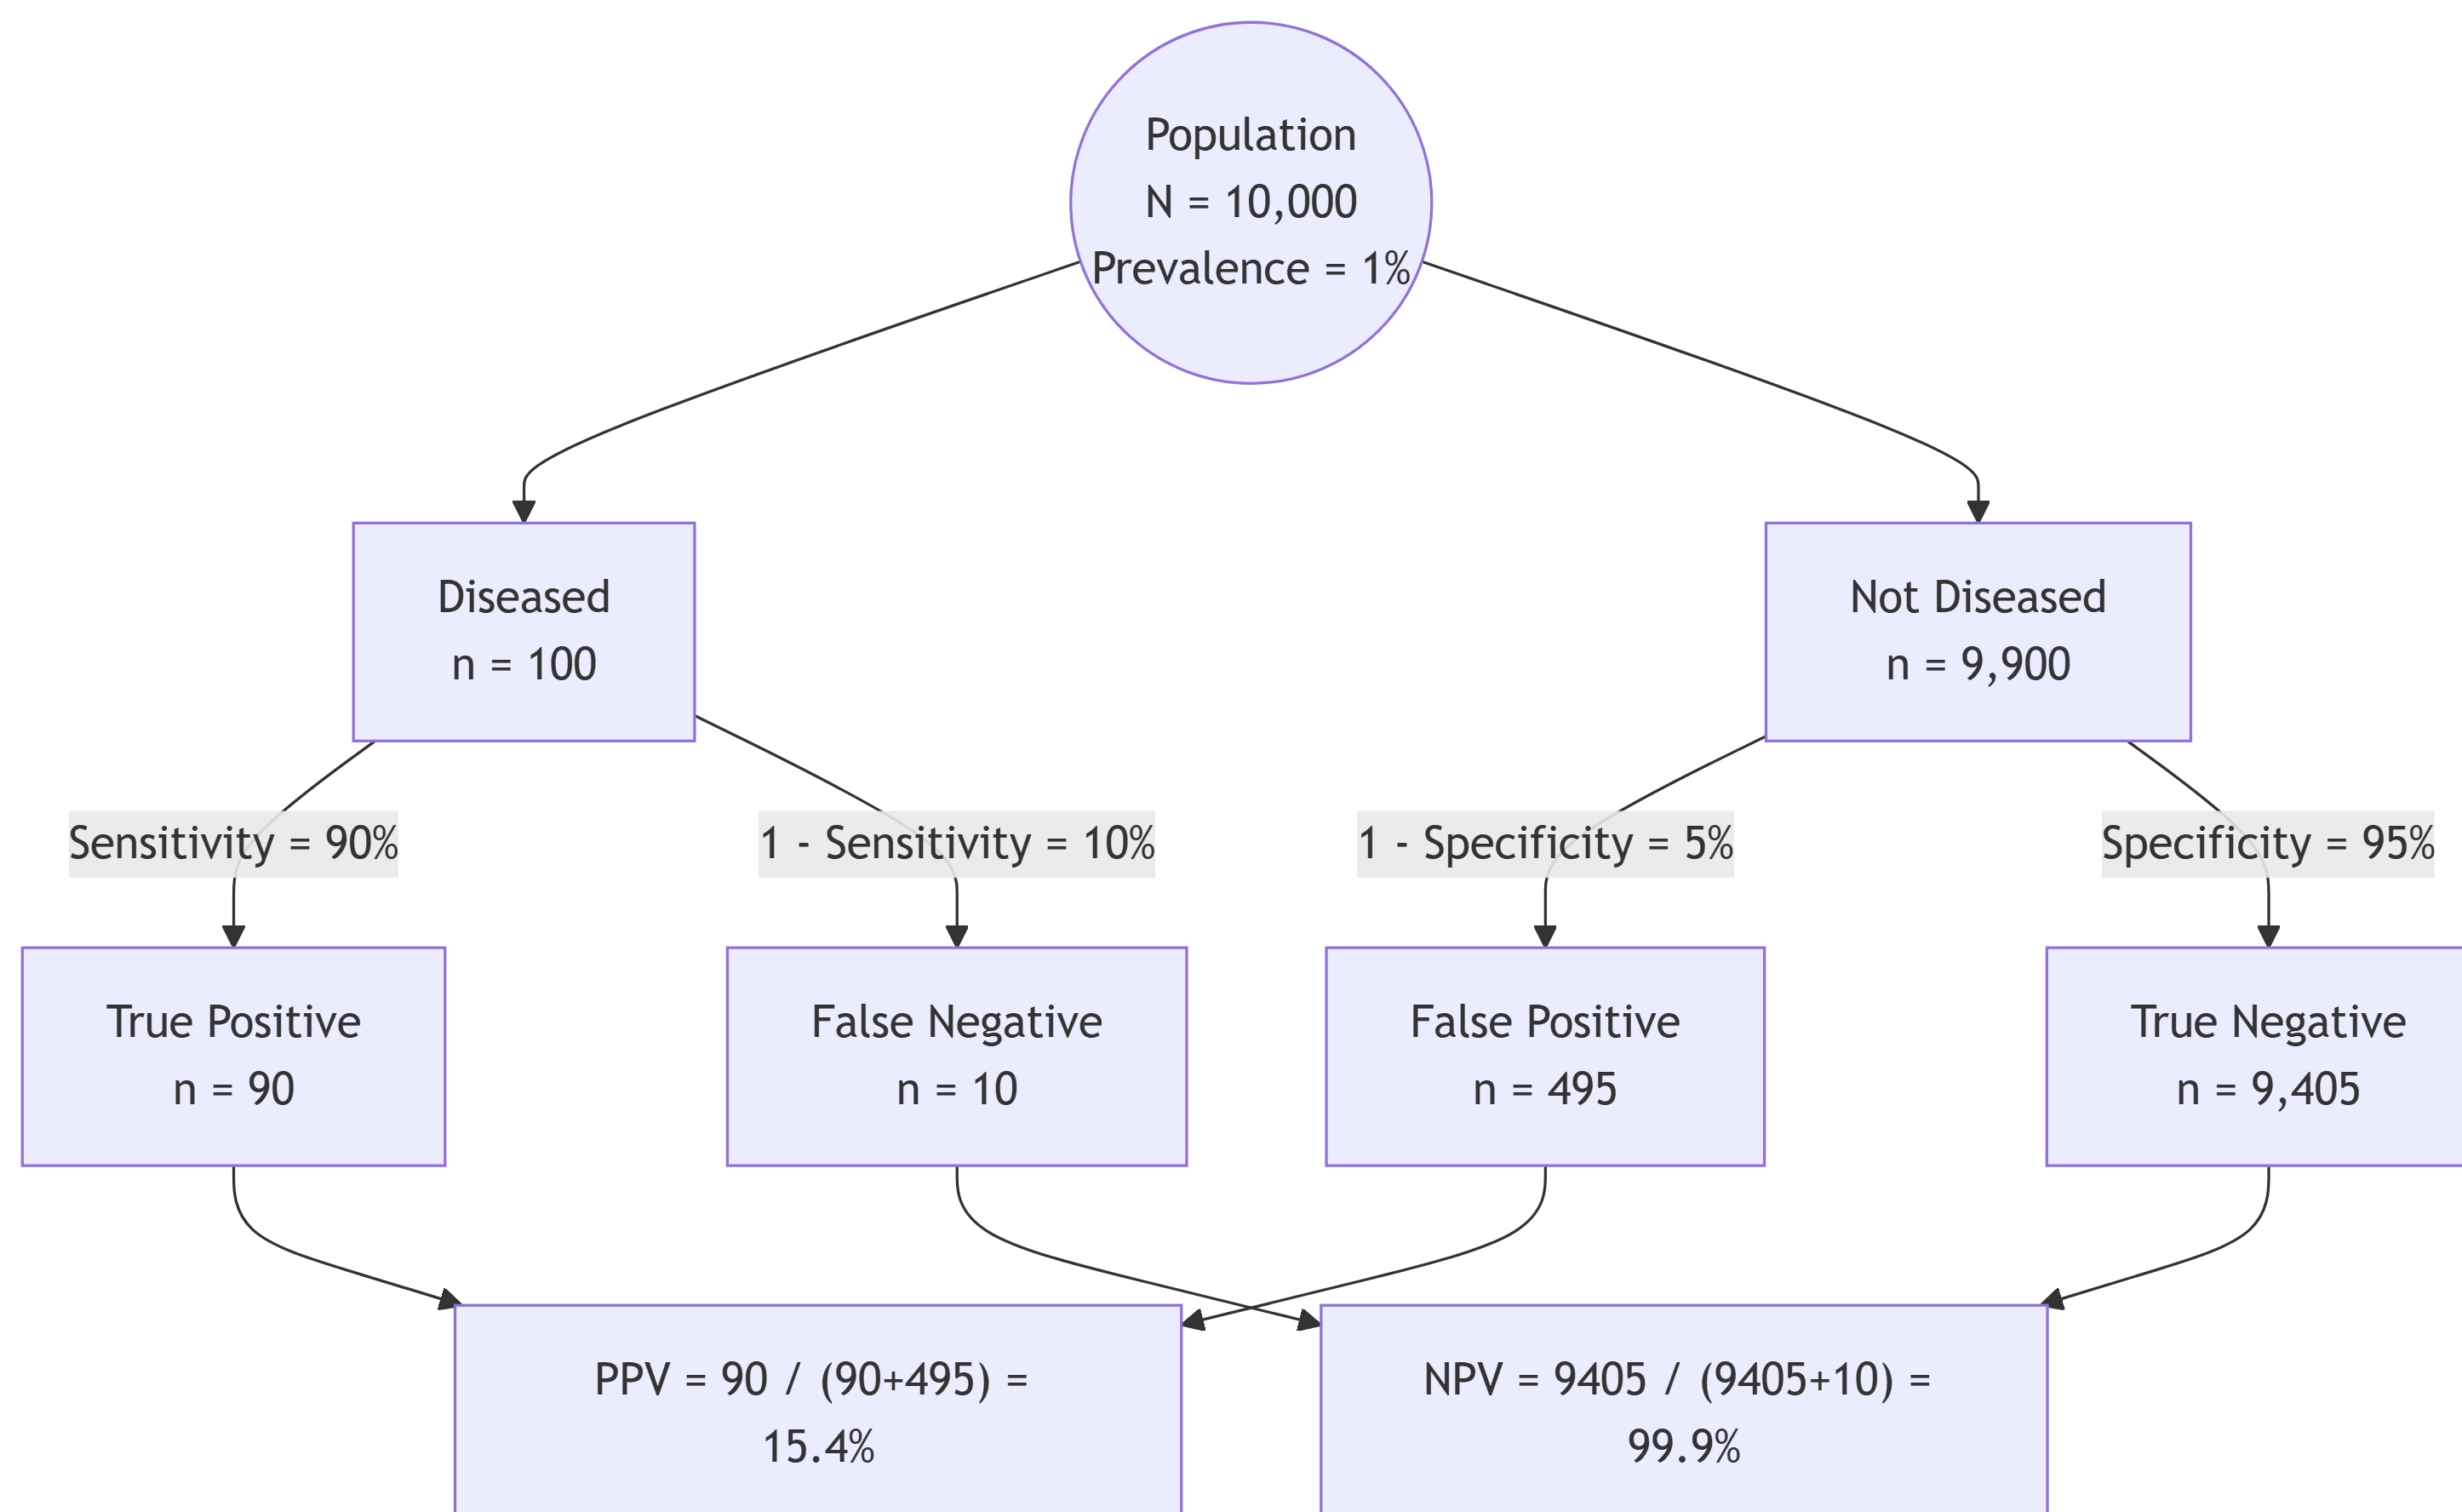
\includegraphics[width=9.37in,height=5.76in]{Section2/04_probability_files/figure-latex/mermaid-figure-2.png}

\section{Additional Worked Example: Public Health Screening Program
Comparison}\label{additional-worked-example-public-health-screening-program-comparison}

Compare the same test (sensitivity 90\%, specificity 95\%) used in two
settings: (1) general community screening, prevalence = 1\%; (2) a
high-risk clinic (e.g., HIV-positive patients, close TB contacts),
prevalence = 20\%.

\textbf{Setting 2 calculation (prevalence = 20\%, per 10,000 screened):}

\textbf{Step 1.} Diseased \(= 0.20\times10{,}000=2000\); Not diseased
\(=8000\).

\textbf{Step 2.} \(TP = 0.90\times2000=1800\); \(FN=200\).

\textbf{Step 3.} \(TN=0.95\times8000=7600\); \(FP=400\).

\textbf{Step 4.} \(PPV = 1800/(1800+400) = 1800/2200 = 0.818 = 81.8\%\).

\begin{longtable}[]{@{}llll@{}}
\toprule\noalign{}
Setting & Prevalence & PPV & NPV \\
\midrule\noalign{}
\endhead
\bottomrule\noalign{}
\endlastfoot
Community screening & 1\% & 15.4\% & 99.9\% \\
High-risk clinic & 20\% & 81.8\% & 97.4\% (calc: \(7600/7800\)) \\
\end{longtable}

\begin{tcolorbox}[enhanced jigsaw, bottomrule=.15mm, breakable, opacityback=0, toptitle=1mm, titlerule=0mm, bottomtitle=1mm, colback=white, arc=.35mm, rightrule=.15mm, toprule=.15mm, leftrule=.75mm, title=\textcolor{quarto-callout-tip-color}{\faLightbulb}\hspace{0.5em}{Tip}, colbacktitle=quarto-callout-tip-color!10!white, colframe=quarto-callout-tip-color-frame, coltitle=black, left=2mm, opacitybacktitle=0.6]

This is why public health screening programs \textbf{target high-risk
subgroups} rather than screening entire low-prevalence populations
indiscriminately, PPV improves dramatically as prevalence rises, even
with an unchanged test.

\end{tcolorbox}

\chapter{Bayesian Inference}\label{bayesian-inference}

Section 5 applied Bayes' Theorem to a binary event (disease
present/absent). \textbf{Bayesian inference} generalizes this idea to
estimate unknown \textbf{parameters} (like a population proportion or
mean), treating them not as fixed unknown constants (as in frequentist
statistics) but as quantities with their own probability distributions
that get updated as data accumulate.

\section{The Core Components}\label{the-core-components}

\subsection{Prior}\label{prior}

The \textbf{prior distribution}, \(P(\theta)\), represents our belief
about a parameter \(\theta\) \textbf{before} observing the current data.
It may come from previous studies, expert opinion, or be deliberately
``uninformative'' (flat) if little is known in advance.

\subsection{Likelihood}\label{likelihood}

The \textbf{likelihood}, \(P(\text{data}|\theta)\), quantifies how
probable the observed data are, for each possible value of the parameter
\(\theta\). It is the same likelihood function used in classical
(frequentist) statistics, e.g., in maximum likelihood estimation.

\subsection{Posterior}\label{posterior}

The \textbf{posterior distribution}, \(P(\theta|\text{data})\),
represents our updated belief about \(\theta\) \textbf{after} combining
the prior with the observed data, via Bayes' Theorem:

\[P(\theta|\text{data}) = \frac{P(\text{data}|\theta)\,P(\theta)}{P(\text{data})} \propto P(\text{data}|\theta)\,P(\theta)\]

In words: \textbf{Posterior} \(\propto\) Likelihood \(\times\) Prior.
The denominator \(P(\text{data})\) is a normalizing constant (the
marginal probability of the data, integrated/summed over all possible
\(\theta\)) that ensures the posterior is a valid probability
distribution.

\subsection{Posterior Predictive
Distribution}\label{posterior-predictive-distribution}

The \textbf{posterior predictive distribution} is the probability
distribution of a \textbf{new, not-yet-observed} data point, averaged
over the uncertainty in the parameter as captured by the posterior
distribution:
\[P(\tilde{y}|\text{data}) = \int P(\tilde{y}|\theta)\,P(\theta|\text{data})\,d\theta\]

Unlike a frequentist prediction that plugs in a single point estimate of
\(\theta\), the posterior predictive distribution properly accounts for
\textbf{both} the inherent randomness in new data \textbf{and} our
remaining uncertainty about \(\theta\) itself --- typically giving
wider, more honest prediction intervals.

\section{Simple Numerical Example --- Estimating a Disease
Prevalence}\label{simple-numerical-example-estimating-a-disease-prevalence}

A researcher wants to estimate the prevalence (\(\theta\)) of a rare
infection in a village. Based on similar villages studied previously,
the researcher's \textbf{prior belief} is centered around 10\%
prevalence, formalized as a Beta distribution:
\(\theta \sim \text{Beta}(2, 18)\) (prior mean \(= 2/(2+18) = 0.10\)).

A sample of \(n = 50\) villagers is tested, and \(x = 8\) test positive
(this is the \textbf{data/likelihood}, modeled as Binomial).

\textbf{Step 1: Prior:} \(\text{Beta}(\alpha=2, \beta=18)\), prior mean
\(=0.10\).

\textbf{Step 2: Likelihood:} Binomial with \(x=8\) successes out of
\(n=50\).

\textbf{Step 3: Posterior:} For a Binomial likelihood with a Beta prior
(a ``conjugate prior'' pair), the posterior is also Beta, with
parameters updated simply by adding the observed successes/failures:
\[\theta|\text{data} \sim \text{Beta}(\alpha + x,\ \beta + n - x) = \text{Beta}(2+8,\ 18+42) = \text{Beta}(10, 60)\]

\textbf{Step 4: Posterior mean:}
\[E[\theta|\text{data}] = \frac{10}{10+60} = \frac{10}{70} = 0.143 = 14.3\%\]

\textbf{Interpretation:} The posterior mean (14.3\%) lies between the
prior mean (10\%) and the raw sample proportion (\(8/50=16\%\)). The
Bayesian estimate is a \textbf{weighted compromise} between prior belief
and observed data, with the weight determined by the relative
``strength'' (sample size) of the prior versus the new data. As more
data accumulate, the posterior increasingly reflects the observed data
and less the prior.

\section{Frequentist vs.~Bayesian
Comparison}\label{frequentist-vs.-bayesian-comparison}

\begin{longtable}[]{@{}
  >{\raggedright\arraybackslash}p{(\linewidth - 4\tabcolsep) * \real{0.3333}}
  >{\raggedright\arraybackslash}p{(\linewidth - 4\tabcolsep) * \real{0.3333}}
  >{\raggedright\arraybackslash}p{(\linewidth - 4\tabcolsep) * \real{0.3333}}@{}}
\toprule\noalign{}
\begin{minipage}[b]{\linewidth}\raggedright
Aspect
\end{minipage} & \begin{minipage}[b]{\linewidth}\raggedright
Frequentist
\end{minipage} & \begin{minipage}[b]{\linewidth}\raggedright
Bayesian
\end{minipage} \\
\midrule\noalign{}
\endhead
\bottomrule\noalign{}
\endlastfoot
View of parameters & Fixed, unknown constants & Random variables with a
probability distribution \\
Uses prior information? & No & Yes, explicitly via the prior
distribution \\
Key output & Point estimate + confidence interval + p-value & Posterior
distribution (full distribution of belief) \\
Interval interpretation & 95\% CI: if we repeated the study infinitely,
95\% of such intervals would contain the true parameter & 95\% Credible
Interval: there is a 95\% probability the true parameter lies in this
interval, given the data and prior \\
Probability interpretation & Long-run frequency of repeatable events &
Degree of belief/uncertainty, updatable with new evidence \\
Handles small samples/rare events well? & Can struggle (e.g., wide,
unstable CIs) & Can incorporate prior knowledge to stabilize
estimates \\
Computational approach & Closed-form formulas, hypothesis tests & Often
requires simulation (e.g., MCMC) for complex models \\
\end{longtable}

\begin{tcolorbox}[enhanced jigsaw, bottomrule=.15mm, breakable, opacityback=0, toptitle=1mm, titlerule=0mm, bottomtitle=1mm, colback=white, arc=.35mm, rightrule=.15mm, toprule=.15mm, leftrule=.75mm, title=\textcolor{quarto-callout-tip-color}{\faLightbulb}\hspace{0.5em}{Tip}, colbacktitle=quarto-callout-tip-color!10!white, colframe=quarto-callout-tip-color-frame, coltitle=black, left=2mm, opacitybacktitle=0.6]

The \textbf{frequentist confidence interval} and the \textbf{Bayesian
credible interval} often look numerically similar (especially with large
samples and uninformative priors), but their \emph{interpretations} are
fundamentally different. The Bayesian interpretation: ``there is a 95\%
probability the parameter lies in this range'' is usually closer to what
people \emph{intuitively} (though incorrectly, in the frequentist
framework) assume a confidence interval means. This distinction is
revisited in Section 11.

\end{tcolorbox}

\section{Applications in
Epidemiology}\label{applications-in-epidemiology}

\begin{itemize}
\tightlist
\item
  \textbf{Disease surveillance:} Updating estimated outbreak size or
  reproduction number (\(R_t\)) in real time as new case data arrive,
  using previous estimates as priors.
\item
  \textbf{Diagnostic test evaluation:} Combining sparse validation data
  with prior information from similar tests to estimate
  sensitivity/specificity, especially useful when validation samples are
  small.
\item
  \textbf{Meta-analysis:} Hierarchical Bayesian models combine evidence
  across multiple studies, treating study-specific effects as drawn from
  a common prior distribution.
\item
  \textbf{Clinical trial monitoring:} Bayesian adaptive designs update
  the probability that a treatment is superior as data accrue, allowing
  trials to stop early for efficacy or futility.
\item
  \textbf{Small-area health estimation:} Bayesian smoothing (e.g.,
  disease mapping) borrows strength from neighboring regions as priors
  to stabilize rate estimates in small populations, where raw rates
  would be highly unstable.
\end{itemize}

\section{Summary}\label{summary-3}

\begin{itemize}
\tightlist
\item
  A random experiment has a defined \textbf{sample space};
  \textbf{events} are subsets of that space.
\item
  The three \textbf{probability axioms} (non-negativity, normalization,
  additivity) form the mathematical foundation of all probability rules.
\item
  Probability can be assigned via the \textbf{classical},
  \textbf{empirical}, or \textbf{subjective} approach depending on the
  situation.
\item
  The \textbf{addition rule} combines ``or'' probabilities; subtract the
  intersection unless events are mutually exclusive.
\item
  The \textbf{multiplication rule} combines ``and'' probabilities; use
  conditional probability unless events are independent.
\item
  \textbf{Conditional probability}, \(P(B|A) = P(A\cap B)/P(A)\), is the
  gateway to Bayes' Theorem, covered next in Section 5.
\item
  Bayes' Theorem, \(P(B|A) = \dfrac{P(A|B)P(B)}{P(A)}\), lets us
  ``reverse'' a conditional probability using the prior probability and
  likelihood.
\item
  In diagnostic testing, Bayes' Theorem converts
  \textbf{sensitivity/specificity} (properties of the test) into
  \textbf{PPV/NPV} (what clinicians and patients actually want to know),
  and critically depends on \textbf{disease prevalence}.
\item
  \textbf{Sensitivity and specificity are independent of prevalence; PPV
  and NPV are not.}
\item
  \textbf{Likelihood ratios} summarize how much a test result shifts the
  probability of disease, independent of prevalence, and can be combined
  with pre-test odds to get post-test odds.
\item
  Bayesian inference combines a \textbf{prior} belief with the
  \textbf{likelihood} of observed data to produce a \textbf{posterior}
  distribution: Posterior \(\propto\) Likelihood \(\times\) Prior.
\item
  The \textbf{posterior predictive distribution} forecasts new data
  while properly accounting for parameter uncertainty.
\item
  Bayesian and frequentist approaches often agree numerically with large
  samples and weak priors, but differ fundamentally in interpretation
  and in their ability to formally incorporate prior information.
\item
  Bayesian methods are increasingly used in epidemiology for
  surveillance, small-area estimation, and adaptive clinical trial
  design.
\end{itemize}

\chapter{Discrete Probability
Distributions}\label{discrete-probability-distributions}

\section{Random Variables}\label{random-variables}

A \textbf{random variable} is a numeric variable whose value is
determined by the outcome of a random experiment. Random variables are
denoted with capital letters (\(X\), \(Y\)) and their specific realized
values with lowercase letters (\(x\), \(y\)).

\begin{itemize}
\tightlist
\item
  A \textbf{discrete random variable} takes a countable number of values
  (finite or countably infinite), e.g., number of ER visits in a month.
\item
  A \textbf{continuous random variable} takes any value within an
  interval (covered in Section 8), e.g., blood pressure.
\end{itemize}

\section{Probability Mass Function
(PMF)}\label{probability-mass-function-pmf}

For a discrete random variable \(X\), the \textbf{probability mass
function (PMF)}, \(P(X=x)\), gives the probability that \(X\) takes on
each specific value \(x\). A valid PMF must satisfy:

\begin{enumerate}
\def\labelenumi{\arabic{enumi}.}
\tightlist
\item
  \(0 \le P(X=x) \le 1\) for every \(x\)
\item
  \(\sum_{\text{all } x} P(X=x) = 1\)
\end{enumerate}

The \textbf{cumulative distribution function (CDF)} is
\(F(x) = P(X \le x) = \sum_{k\le x} P(X=k)\).

\section{Expected Value}\label{expected-value}

The \textbf{expected value} (mean) of a discrete random variable is the
long-run average value, weighted by probability:
\[E(X) = \mu = \sum_{\text{all } x} x\, P(X=x)\]

\section{Variance}\label{variance-2}

\[Var(X) = \sigma^2 = \sum_{\text{all }x}(x-\mu)^2 P(X=x) = E(X^2) - [E(X)]^2\]

\textbf{Worked example:} A community health worker screens patients. let
\(X\) = number of positive screens out of the first 3 patients tested,
with PMF:

\(P(0)=0.20\)

\(P(1)=0.35\)

\(P(2)=0.30\)

\(P(3)=0.15\)

\textbf{Step 1:} Verify PMF sums to 1:

\(0.20+0.35+0.30+0.15=1.00\)

\textbf{Step 2:}
\(E(X) = 0(0.20)+1(0.35)+2(0.30)+3(0.15) = 0+0.35+0.60+0.45=1.40\)

\textbf{Step
3:}\(E(X^2) = 0^2(0.20)+1^2(0.35)+2^2(0.30)+3^2(0.15)=0+0.35+1.20+1.35=2.90\)

\textbf{Step 4:}

\(Var(X) = 2.90-1.40^2=2.90-1.96=0.94\)

\(SD(X)=\sqrt{0.94}=0.97\).

\begin{center}\rule{0.5\linewidth}{0.5pt}\end{center}

\section{Bernoulli Distribution}\label{bernoulli-distribution}

\subsection{Definition}\label{definition-11}

Models a \textbf{single trial} with exactly two possible outcomes:
``success'' (1) or ``failure'' (0).

\subsection{PMF}\label{pmf}

\[P(X=x) = p^x(1-p)^{1-x}, \quad x \in \{0,1\}\]

\subsection{Parameters, Mean, Variance}\label{parameters-mean-variance}

\begin{longtable}[]{@{}ll@{}}
\toprule\noalign{}
Parameter & \(p\) = probability of success \\
\midrule\noalign{}
\endhead
\bottomrule\noalign{}
\endlastfoot
Mean & \(E(X) = p\) \\
Variance & \(Var(X) = p(1-p)\) \\
\end{longtable}

\textbf{Derivation of mean:}

\(E(X) = 0\cdot(1-p) + 1\cdot p = p\)

\textbf{Derivation of variance:}

\(E(X^2) = 0^2(1-p)+1^2(p) = p\)

\(Var(X) = E(X^2)-[E(X)]^2 = p-p^2=p(1-p)\).

\subsection{Shape \& Assumptions}\label{shape-assumptions}

\begin{itemize}
\item
  Two-point distribution
\item
  Shape depends entirely on \(p\).
\item
  Assumes a single trial with a fixed success probability.
\end{itemize}

\subsection{Applications / Public Health
Example}\label{applications-public-health-example}

Whether a single patient tests positive for a disease (\(p\) =
prevalence); whether a single newborn is preterm; the building block for
the Binomial distribution.

\subsection{R Code and Graph}\label{r-code-and-graph}

\begin{Shaded}
\begin{Highlighting}[]
\NormalTok{p }\OtherTok{\textless{}{-}} \FloatTok{0.3}
\NormalTok{x }\OtherTok{\textless{}{-}} \FunctionTok{c}\NormalTok{(}\DecValTok{0}\NormalTok{, }\DecValTok{1}\NormalTok{)}
\NormalTok{prob }\OtherTok{\textless{}{-}} \FunctionTok{dbinom}\NormalTok{(x, }\AttributeTok{size =} \DecValTok{1}\NormalTok{, }\AttributeTok{prob =}\NormalTok{ p)}
\FunctionTok{ggplot}\NormalTok{(}\FunctionTok{data.frame}\NormalTok{(}\AttributeTok{x =} \FunctionTok{factor}\NormalTok{(x), prob), }\FunctionTok{aes}\NormalTok{(x, prob)) }\SpecialCharTok{+}
  \FunctionTok{geom\_col}\NormalTok{(}\AttributeTok{fill =} \StringTok{"steelblue"}\NormalTok{) }\SpecialCharTok{+}
  \FunctionTok{labs}\NormalTok{(}\AttributeTok{title =} \StringTok{"Bernoulli(p = 0.3)"}\NormalTok{, }\AttributeTok{x =} \StringTok{"X"}\NormalTok{, }\AttributeTok{y =} \StringTok{"P(X = x)"}\NormalTok{) }\SpecialCharTok{+}
  \FunctionTok{theme\_minimal}\NormalTok{()}
\end{Highlighting}
\end{Shaded}

\begin{center}
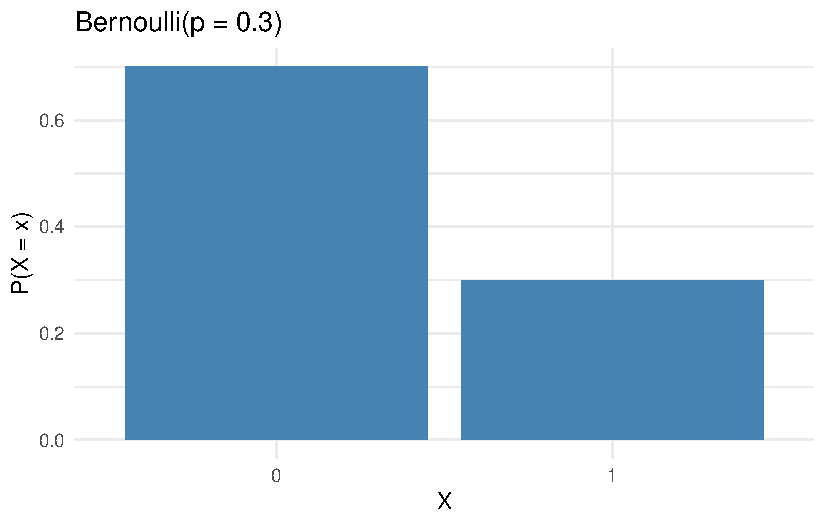
\includegraphics[width=0.85\linewidth,height=\textheight,keepaspectratio]{Section2/05_discrete_probability_distributions_files/figure-pdf/bernoulli-1.pdf}
\end{center}

\subsection{Manual Calculation}\label{manual-calculation-5}

If prevalence of a risk factor 30\% (\(p = 0.30\)).

\(P(X=1) = 0.30\)

\(P(X=0)=0.70\)

Mean \(=0.30\)

Variance \(=0.30(0.70)=0.21\)

\begin{center}\rule{0.5\linewidth}{0.5pt}\end{center}

\section{Binomial Distribution}\label{binomial-distribution}

\subsection{Definition}\label{definition-12}

Models the number of \textbf{successes in} \(n\) independent Bernoulli
trials, each with the same probability of success \(p\).

\subsection{PMF}\label{pmf-1}

\[P(X=x) = \binom{n}{x}p^x(1-p)^{n-x}, \quad x=0,1,\ldots,n\]

where \(\binom{n}{x} = \dfrac{n!}{x!(n-x)!}\).

\subsection{Parameters, Mean,
Variance}\label{parameters-mean-variance-1}

\begin{longtable}[]{@{}ll@{}}
\toprule\noalign{}
Parameter & \(n\) = number of trials, \(p\) = probability of success \\
\midrule\noalign{}
\endhead
\bottomrule\noalign{}
\endlastfoot
Mean & \(E(X) = np\) \\
Variance & \(Var(X) = np(1-p)\) \\
\end{longtable}

\subsection{Shape}\label{shape}

\begin{itemize}
\item
  Symmetric when \(p=0.5\)
\item
  Right-skewed when \(p<0.5\) and left-skewed when \(p>0.5\)
\item
  Approaches a Normal shape as \(n\) grows (for fixed \(p\) not too
  close to 0 or 1). It is a consequence of the Central Limit Theorem.
\end{itemize}

\subsection{Assumptions}\label{assumptions}

\begin{enumerate}
\def\labelenumi{\arabic{enumi}.}
\tightlist
\item
  Fixed number of trials \(n\).
\item
  Each trial has only two outcomes.
\item
  Constant probability of success \(p\) across trials.
\item
  Trials are independent.
\end{enumerate}

\subsection{Applications / Public Health
Example}\label{applications-public-health-example-1}

Number of patients who respond to treatment out of \(n\) treated; number
of children vaccinated out of \(n\) eligible; number of surgical-site
infections out of \(n\) surgeries.

\subsection{R Code and Graph}\label{r-code-and-graph-1}

\begin{Shaded}
\begin{Highlighting}[]
\NormalTok{n }\OtherTok{\textless{}{-}} \DecValTok{20}\NormalTok{; p }\OtherTok{\textless{}{-}} \FloatTok{0.3}
\NormalTok{x }\OtherTok{\textless{}{-}} \DecValTok{0}\SpecialCharTok{:}\NormalTok{n}
\NormalTok{prob }\OtherTok{\textless{}{-}} \FunctionTok{dbinom}\NormalTok{(x, }\AttributeTok{size =}\NormalTok{ n, }\AttributeTok{prob =}\NormalTok{ p)}
\FunctionTok{ggplot}\NormalTok{(}\FunctionTok{data.frame}\NormalTok{(x, prob), }\FunctionTok{aes}\NormalTok{(x, prob)) }\SpecialCharTok{+}
  \FunctionTok{geom\_col}\NormalTok{(}\AttributeTok{fill =} \StringTok{"darkorange"}\NormalTok{) }\SpecialCharTok{+}
  \FunctionTok{labs}\NormalTok{(}\AttributeTok{title =} \StringTok{"Binomial(n = 20, p = 0.3)"}\NormalTok{, }\AttributeTok{x =} \StringTok{"Number of successes"}\NormalTok{, }\AttributeTok{y =} \StringTok{"P(X = x)"}\NormalTok{) }\SpecialCharTok{+}
  \FunctionTok{theme\_minimal}\NormalTok{()}
\end{Highlighting}
\end{Shaded}

\begin{center}
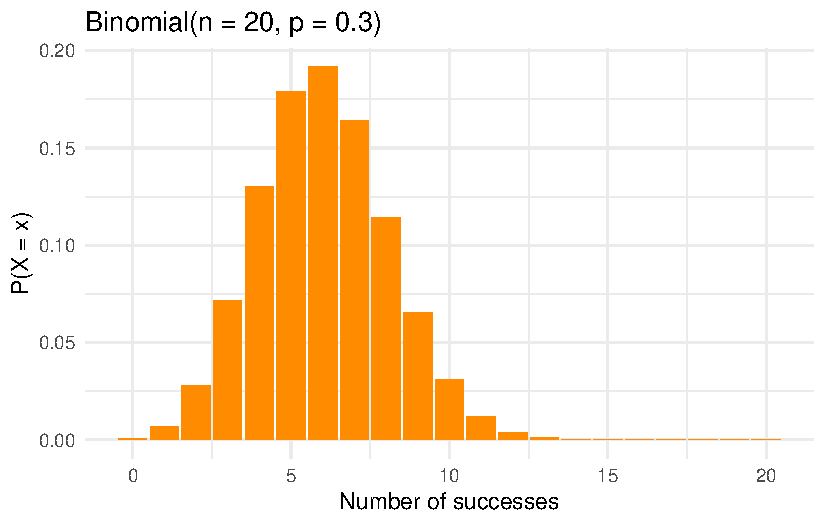
\includegraphics[width=0.85\linewidth,height=\textheight,keepaspectratio]{Section2/05_discrete_probability_distributions_files/figure-pdf/binomial-1.pdf}
\end{center}

\subsection{Worked Example (Manual
Calculation)}\label{worked-example-manual-calculation}

In a clinic, 30\% of screened patients (\(p=0.3\)) are found to have
elevated cholesterol. Out of \(n=5\) patients screened today, what is
the probability exactly 2 have elevated cholesterol?

\textbf{Step 1:} Identify \(n=5\), \(x=2\), \(p=0.3\)

\textbf{Step 2:} Compute the binomial coefficient:
\(\binom{5}{2} = \dfrac{5!}{2!3!} = \dfrac{120}{2\times 6}=10\)

\textbf{Step 3:} Compute \(p^x = 0.3^2 = 0.09\) and
\((1-p)^{n-x} = 0.7^3=0.343\).

\textbf{Step 4:} Multiply:
\[P(X=2) = 10 \times 0.09 \times 0.343 = 0.3087 \approx 30.9\%\]

\textbf{Verification in R:}
\texttt{dbinom(2,\ size\ =\ 5,\ prob\ =\ 0.3)} returns 0.3087.

Mean \(= np = 5(0.3) = 1.5\) patients

Variance \(= np(1-p)=5(0.3)(0.7)=1.05\)

\begin{center}\rule{0.5\linewidth}{0.5pt}\end{center}

\section{Geometric Distribution}\label{geometric-distribution}

\subsection{Definition}\label{definition-13}

Models the \textbf{number of trials needed to obtain the first success}
in a sequence of independent Bernoulli trials.

\subsection{PMF}\label{pmf-2}

\[P(X=x) = (1-p)^{x-1}p, \quad x=1,2,3,\ldots\]

(Convention: \(X\) counts the trial \emph{on which} the first success
occurs. An alternative parameterization counts the number of
\emph{failures before} the first success, \(Y=X-1\).)

\subsection{Parameters, Mean,
Variance}\label{parameters-mean-variance-2}

\begin{longtable}[]{@{}ll@{}}
\toprule\noalign{}
Parameter & \(p\) = probability of success per trial \\
\midrule\noalign{}
\endhead
\bottomrule\noalign{}
\endlastfoot
Mean & \(E(X) = \dfrac{1}{p}\) \\
Variance & \(Var(X) = \dfrac{1-p}{p^2}\) \\
\end{longtable}

\subsection{Shape \& Assumptions}\label{shape-assumptions-1}

\begin{itemize}
\item
  Always right-skewed
\item
  Highest probability at \(x=1\), decreasing geometrically thereafter.
\item
  Assumes independent trials with constant \(p\), continuing until the
  first success (a ``waiting time'' distribution).
\end{itemize}

\subsection{Applications / Public Health
Example}\label{applications-public-health-example-2}

\begin{itemize}
\tightlist
\item
  Number of couples' pregnancy attempts (cycles) until conception
\end{itemize}

\begin{itemize}
\item
  Number of blood donors screened until finding one with a specific rare
  blood type
\item
  Number of contact-tracing attempts until successfully reaching a
  contact.
\end{itemize}

\subsection{R Code and Graph}\label{r-code-and-graph-2}

\begin{Shaded}
\begin{Highlighting}[]
\NormalTok{p }\OtherTok{\textless{}{-}} \FloatTok{0.25}
\NormalTok{x }\OtherTok{\textless{}{-}} \DecValTok{1}\SpecialCharTok{:}\DecValTok{15}
\NormalTok{prob }\OtherTok{\textless{}{-}} \FunctionTok{dgeom}\NormalTok{(x }\SpecialCharTok{{-}} \DecValTok{1}\NormalTok{, }\AttributeTok{prob =}\NormalTok{ p)  }\CommentTok{\# R\textquotesingle{}s dgeom counts failures before success}
\FunctionTok{ggplot}\NormalTok{(}\FunctionTok{data.frame}\NormalTok{(x, prob), }\FunctionTok{aes}\NormalTok{(x, prob)) }\SpecialCharTok{+}
  \FunctionTok{geom\_col}\NormalTok{(}\AttributeTok{fill =} \StringTok{"seagreen"}\NormalTok{) }\SpecialCharTok{+}
  \FunctionTok{labs}\NormalTok{(}\AttributeTok{title =} \StringTok{"Geometric(p = 0.25), X = trial of first success"}\NormalTok{,}
       \AttributeTok{x =} \StringTok{"Trial number of first success"}\NormalTok{, }\AttributeTok{y =} \StringTok{"P(X = x)"}\NormalTok{) }\SpecialCharTok{+}
  \FunctionTok{theme\_minimal}\NormalTok{()}
\end{Highlighting}
\end{Shaded}

\begin{center}
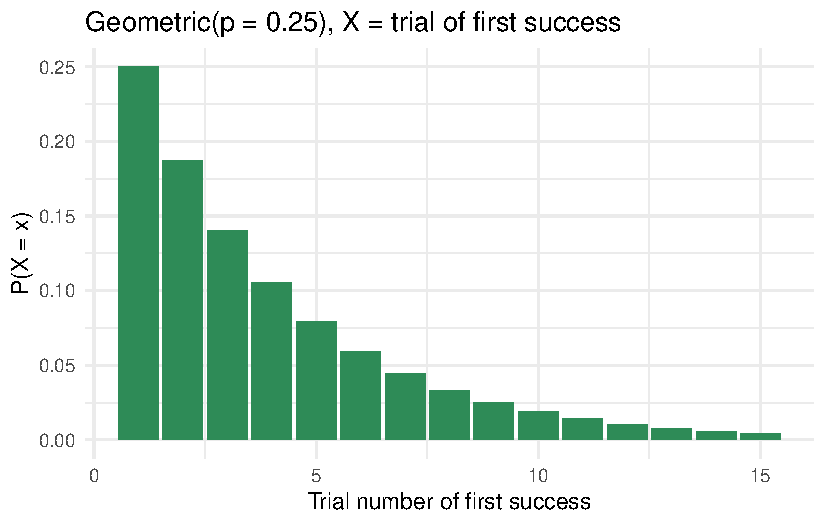
\includegraphics[width=0.85\linewidth,height=\textheight,keepaspectratio]{Section2/05_discrete_probability_distributions_files/figure-pdf/geometric-1.pdf}
\end{center}

\begin{tcolorbox}[enhanced jigsaw, bottomrule=.15mm, breakable, opacityback=0, toptitle=1mm, titlerule=0mm, bottomtitle=1mm, colback=white, arc=.35mm, rightrule=.15mm, toprule=.15mm, leftrule=.75mm, title=\textcolor{quarto-callout-tip-color}{\faLightbulb}\hspace{0.5em}{Tip}, colbacktitle=quarto-callout-tip-color!10!white, colframe=quarto-callout-tip-color-frame, coltitle=black, left=2mm, opacitybacktitle=0.6]

R's \texttt{dgeom(k,\ prob)} defines \(k\) as the number of
\textbf{failures before} the first success, so to match the ``trial
number'' parameterization above, use \texttt{dgeom(x\ -\ 1,\ prob)}.

\end{tcolorbox}

\subsection{Worked Example (Manual
Calculation)}\label{worked-example-manual-calculation-1}

If 25\% of blood donors (\(p=0.25\)) have blood type O-negative, what is
the probability that the \textbf{4th} donor screened is the first one
with O-negative blood?

\textbf{Step 1:}

\(x=4\), \(p=0.25\), so \(1-p=0.75\)

\textbf{Step 2:} Apply the PMF\\
\[P(X=4) = (0.75)^{3}(0.25) = 0.4219\times0.25 = 0.1055 \approx 10.6\%\]

\textbf{Mean} \(= 1/0.25 = 4\) donors (on average, expect to screen 4
donors to find one O-negative).

\textbf{Variance} \(= (1-0.25)/0.25^2 = 0.75/0.0625=12\).

\begin{center}\rule{0.5\linewidth}{0.5pt}\end{center}

\section{Negative Binomial
Distribution}\label{negative-binomial-distribution}

\subsection{Definition}\label{definition-14}

Generalizes the Geometric distribution: models the \textbf{number of
trials needed to achieve the} \(r\)-th success.

\subsection{PMF}\label{pmf-3}

\[P(X=x) = \binom{x-1}{r-1}p^r(1-p)^{x-r}, \quad x=r,r+1,r+2,\ldots\]

\subsection{Parameters, Mean,
Variance}\label{parameters-mean-variance-3}

\begin{longtable}[]{@{}
  >{\raggedright\arraybackslash}p{(\linewidth - 2\tabcolsep) * \real{0.3380}}
  >{\raggedright\arraybackslash}p{(\linewidth - 2\tabcolsep) * \real{0.6620}}@{}}
\toprule\noalign{}
\begin{minipage}[b]{\linewidth}\raggedright
Parameter
\end{minipage} & \begin{minipage}[b]{\linewidth}\raggedright
\(r\) = target number of successes, \(p\) = probability of success per
trial
\end{minipage} \\
\midrule\noalign{}
\endhead
\bottomrule\noalign{}
\endlastfoot
Mean & \(E(X) = \dfrac{r}{p}\) \\
Variance & \(Var(X) = \dfrac{r(1-p)}{p^2}\) \\
\end{longtable}

\subsection{Shape \& Assumptions}\label{shape-assumptions-2}

\begin{itemize}
\item
  Right-skewed (less so as \(r\) increases)
\item
  Same independence/constant-\(p\) assumptions as the Geometric
  distribution (which is the special case \(r=1\)).
\item
  Also widely used (in its alternative ``count'' parameterization) to
  model \textbf{overdispersed count data}, count data whose variance
  exceeds its mean, which the Poisson distribution cannot accommodate.
\end{itemize}

\subsection{Applications / Public Health
Example}\label{applications-public-health-example-3}

\begin{itemize}
\item
  Number of patients that must be screened to identify \(r=3\) cases of
  a rare disease for a case series.
\item
  Modeling overdispersed disease counts (e.g., hospital readmission
  counts) where a Poisson model underestimates variability.
\end{itemize}

\subsection{R Code and Graph}\label{r-code-and-graph-3}

\begin{Shaded}
\begin{Highlighting}[]
\NormalTok{r }\OtherTok{\textless{}{-}} \DecValTok{3}\NormalTok{; p }\OtherTok{\textless{}{-}} \FloatTok{0.25}
\NormalTok{x }\OtherTok{\textless{}{-}}\NormalTok{ r}\SpecialCharTok{:}\DecValTok{30}
\NormalTok{prob }\OtherTok{\textless{}{-}} \FunctionTok{dnbinom}\NormalTok{(x }\SpecialCharTok{{-}}\NormalTok{ r, }\AttributeTok{size =}\NormalTok{ r, }\AttributeTok{prob =}\NormalTok{ p)  }\CommentTok{\# R counts failures before r{-}th success}
\FunctionTok{ggplot}\NormalTok{(}\FunctionTok{data.frame}\NormalTok{(x, prob), }\FunctionTok{aes}\NormalTok{(x, prob)) }\SpecialCharTok{+}
  \FunctionTok{geom\_col}\NormalTok{(}\AttributeTok{fill =} \StringTok{"purple"}\NormalTok{) }\SpecialCharTok{+}
  \FunctionTok{labs}\NormalTok{(}\AttributeTok{title =} \StringTok{"Negative Binomial(r = 3, p = 0.25)"}\NormalTok{,}
       \AttributeTok{x =} \StringTok{"Trial of 3rd success"}\NormalTok{, }\AttributeTok{y =} \StringTok{"P(X = x)"}\NormalTok{) }\SpecialCharTok{+}
  \FunctionTok{theme\_minimal}\NormalTok{()}
\end{Highlighting}
\end{Shaded}

\begin{center}
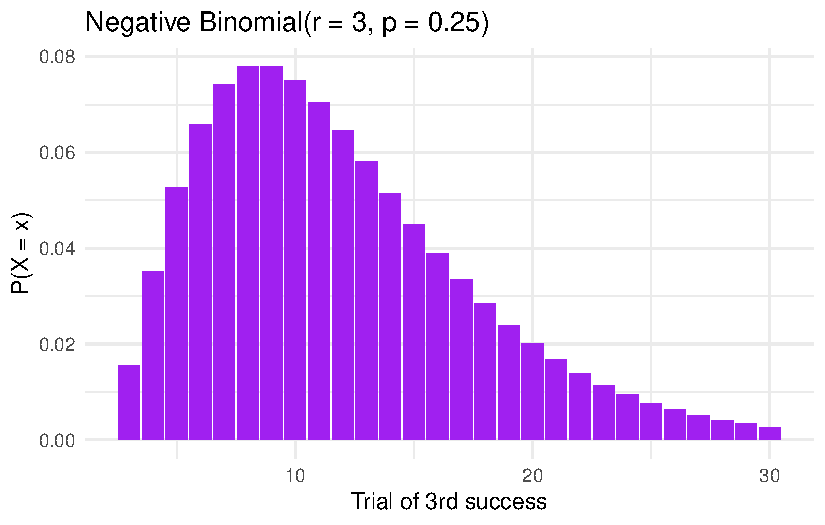
\includegraphics[width=0.85\linewidth,height=\textheight,keepaspectratio]{Section2/05_discrete_probability_distributions_files/figure-pdf/negbinom-1.pdf}
\end{center}

\subsection{Worked Example (Manual
Calculation)}\label{worked-example-manual-calculation-2}

Continuing the O-negative blood donor example (\(p=0.25\)): what is the
probability that the \textbf{6th} donor screened is the one who provides
the \textbf{3rd} O-negative unit found (\(r=3\))?

\textbf{Step 1:}

\(x=6\), \(r=3\), \(p=0.25\)

\textbf{Step 2:}

Binomial coefficient: \(\binom{x-1}{r-1} = \binom{5}{2} = 10\)

\textbf{Step 3:}

\(p^r = 0.25^3 = 0.015625\)

\((1-p)^{x-r} = 0.75^3 = 0.421875\)

\textbf{Step 4:}
\[P(X=6) = 10\times 0.015625\times 0.421875 = 0.0659 \approx 6.6\%\]

Mean \(= r/p = 3/0.25=12\) donors expected to find 3 O-negative units.

\begin{center}\rule{0.5\linewidth}{0.5pt}\end{center}

\section{Hypergeometric Distribution}\label{hypergeometric-distribution}

\subsection{Definition}\label{definition-15}

Models the number of successes in \(n\) draws \textbf{without
replacement} from a finite population of size \(N\) containing \(K\)
successes, used when sampling is done \textbf{without replacement} from
a small, finite population (in contrast to the Binomial, which assumes
independence/replacement).

\subsection{PMF}\label{pmf-4}

\[P(X=x) = \frac{\binom{K}{x}\binom{N-K}{n-x}}{\binom{N}{n}}\]

\subsection{Parameters, Mean,
Variance}\label{parameters-mean-variance-4}

\begin{longtable}[]{@{}
  >{\raggedright\arraybackslash}p{(\linewidth - 2\tabcolsep) * \real{0.3611}}
  >{\raggedright\arraybackslash}p{(\linewidth - 2\tabcolsep) * \real{0.6389}}@{}}
\toprule\noalign{}
\begin{minipage}[b]{\linewidth}\raggedright
Parameter
\end{minipage} & \begin{minipage}[b]{\linewidth}\raggedright
\(N\) = population size, \(K\) = number of successes in population,
\(n\) = sample size
\end{minipage} \\
\midrule\noalign{}
\endhead
\bottomrule\noalign{}
\endlastfoot
Mean & \(E(X) = n\dfrac{K}{N}\) \\
Variance &
\(Var(X) = n\dfrac{K}{N}\cdot\dfrac{N-K}{N}\cdot\dfrac{N-n}{N-1}\) \\
\end{longtable}

The variance formula includes the \textbf{finite population correction
factor}, \(\dfrac{N-n}{N-1}\), which distinguishes it from the Binomial.

\subsection{Shape \& Assumptions}\label{shape-assumptions-3}

\begin{itemize}
\item
  Similar in shape to the Binomial for large \(N\) relative to \(n\) (in
  fact, the Hypergeometric converges to the Binomial as \(N\to\infty\)
  with \(K/N=p\) fixed).
\item
  Assumes sampling \textbf{without replacement} from a finite, known
  population.
\end{itemize}

\subsection{Applications / Public Health
Example}\label{applications-public-health-example-4}

Selecting a sample of vials for quality control from a finite batch (as
in Section 4's defective-vial example); selecting a committee/sample
from a small finite roster of patients with known disease status;
capture-recapture population size estimation.

\subsection{R Code and Graph}\label{r-code-and-graph-4}

\begin{Shaded}
\begin{Highlighting}[]
\NormalTok{N }\OtherTok{\textless{}{-}} \DecValTok{50}\NormalTok{; K }\OtherTok{\textless{}{-}} \DecValTok{10}\NormalTok{; n }\OtherTok{\textless{}{-}} \DecValTok{8}
\NormalTok{x }\OtherTok{\textless{}{-}} \DecValTok{0}\SpecialCharTok{:}\FunctionTok{min}\NormalTok{(n, K)}
\NormalTok{prob }\OtherTok{\textless{}{-}} \FunctionTok{dhyper}\NormalTok{(x, }\AttributeTok{m =}\NormalTok{ K, }\AttributeTok{n =}\NormalTok{ N }\SpecialCharTok{{-}}\NormalTok{ K, }\AttributeTok{k =}\NormalTok{ n)}
\FunctionTok{ggplot}\NormalTok{(}\FunctionTok{data.frame}\NormalTok{(x, prob), }\FunctionTok{aes}\NormalTok{(x, prob)) }\SpecialCharTok{+}
  \FunctionTok{geom\_col}\NormalTok{(}\AttributeTok{fill =} \StringTok{"firebrick"}\NormalTok{) }\SpecialCharTok{+}
  \FunctionTok{labs}\NormalTok{(}\AttributeTok{title =} \StringTok{"Hypergeometric(N=50, K=10, n=8)"}\NormalTok{, }\AttributeTok{x =} \StringTok{"Number of successes"}\NormalTok{, }\AttributeTok{y =} \StringTok{"P(X = x)"}\NormalTok{) }\SpecialCharTok{+}
  \FunctionTok{theme\_minimal}\NormalTok{()}
\end{Highlighting}
\end{Shaded}

\begin{center}
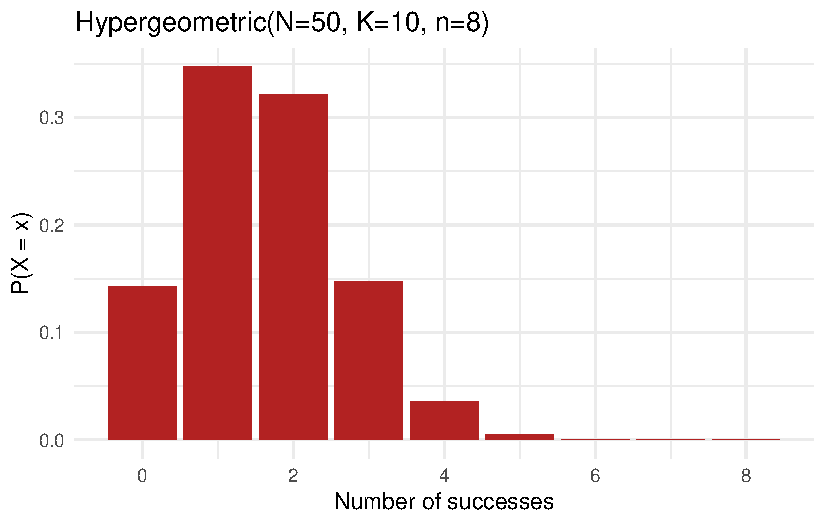
\includegraphics[width=0.85\linewidth,height=\textheight,keepaspectratio]{Section2/05_discrete_probability_distributions_files/figure-pdf/hypergeom-1.pdf}
\end{center}

\subsection{Worked Example (Manual
Calculation)}\label{worked-example-manual-calculation-3}

A batch of \(N=50\) vaccine vials contains \(K=10\) expired vials. A
quality inspector randomly selects \(n=5\) vials for testing (without
replacement). What is the probability exactly \(x=2\) are expired?

\textbf{Step 1:}

\(\binom{K}{x} = \binom{10}{2} = 45\)

\textbf{Step 2:}

\(\binom{N-K}{n-x} = \binom{40}{3} = 9880\)

\textbf{Step 3:}

\(\binom{N}{n} = \binom{50}{5} = 2{,}118{,}760\)

\textbf{Step 4:}
\[P(X=2) = \frac{45\times9880}{2{,}118{,}760} = \frac{444{,}600}{2{,}118{,}760}=0.2099\approx21.0\%\]

Mean \(= n(K/N) = 5(10/50)=1.0\) expired vial expected in the sample.

\begin{center}\rule{0.5\linewidth}{0.5pt}\end{center}

\section{Poisson Distribution}\label{poisson-distribution}

\subsection{Definition}\label{definition-16}

Models the number of \textbf{rare, independent events occurring in a
fixed interval} of time, space, or exposure, when events happen at a
constant average rate \(\lambda\).

\subsection{PMF}\label{pmf-5}

\[P(X=x) = \frac{e^{-\lambda}\lambda^x}{x!}, \quad x=0,1,2,\ldots\]

\subsection{Parameters, Mean,
Variance}\label{parameters-mean-variance-5}

\begin{longtable}[]{@{}ll@{}}
\toprule\noalign{}
Parameter & \(\lambda\) = mean (and rate) of events per interval \\
\midrule\noalign{}
\endhead
\bottomrule\noalign{}
\endlastfoot
Mean & \(E(X) = \lambda\) \\
Variance & \(Var(X) = \lambda\) \\
\end{longtable}

The Poisson is unique in that its \textbf{mean equals its variance}, an
assumption that is often violated in real disease-count data
(overdispersion), motivating the use of the Negative Binomial as an
alternative.

\subsection{Shape \& Assumptions}\label{shape-assumptions-4}

\begin{itemize}
\item
  Right-skewed for small \(\lambda\), approaching a symmetric,
  Normal-like shape as \(\lambda\) increases.
\item
  Assumes:

  \begin{itemize}
  \item
    events occur independently,
  \item
    at a constant average rate,
  \item
    two events cannot occur at exactly the same instant,
  \item
    the number of events in non-overlapping intervals is independent.
  \end{itemize}
\end{itemize}

\subsection{Applications / Public Health
Example}\label{applications-public-health-example-5}

Number of new cases of a rare disease reported per month in a district;
number of hospital-acquired infections per 1000 patient-days; number of
deaths from a rare adverse drug reaction; number of disease outbreaks
per year in a region. The Poisson also arises as the limiting
distribution of the Binomial when \(n\) is large, \(p\) is small, and
\(np=\lambda\) is moderate (the ``law of rare events'').

\subsection{R Code and Graph}\label{r-code-and-graph-5}

\begin{Shaded}
\begin{Highlighting}[]
\NormalTok{lambda }\OtherTok{\textless{}{-}} \DecValTok{4}
\NormalTok{x }\OtherTok{\textless{}{-}} \DecValTok{0}\SpecialCharTok{:}\DecValTok{15}
\NormalTok{prob }\OtherTok{\textless{}{-}} \FunctionTok{dpois}\NormalTok{(x, }\AttributeTok{lambda =}\NormalTok{ lambda)}
\FunctionTok{ggplot}\NormalTok{(}\FunctionTok{data.frame}\NormalTok{(x, prob), }\FunctionTok{aes}\NormalTok{(x, prob)) }\SpecialCharTok{+}
  \FunctionTok{geom\_col}\NormalTok{(}\AttributeTok{fill =} \StringTok{"slateblue"}\NormalTok{) }\SpecialCharTok{+}
  \FunctionTok{labs}\NormalTok{(}\AttributeTok{title =} \StringTok{"Poisson(lambda = 4)"}\NormalTok{, }\AttributeTok{x =} \StringTok{"Number of events"}\NormalTok{, }\AttributeTok{y =} \StringTok{"P(X = x)"}\NormalTok{) }\SpecialCharTok{+}
  \FunctionTok{theme\_minimal}\NormalTok{()}
\end{Highlighting}
\end{Shaded}

\begin{center}
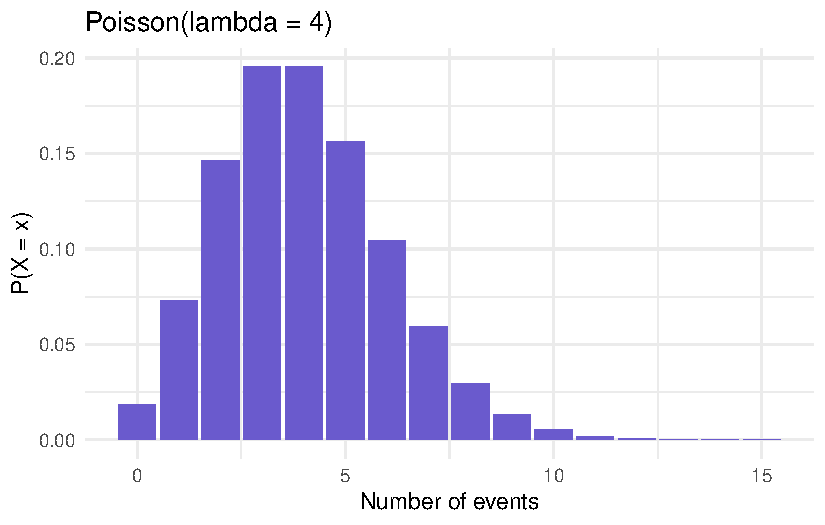
\includegraphics[width=0.85\linewidth,height=\textheight,keepaspectratio]{Section2/05_discrete_probability_distributions_files/figure-pdf/poisson-1.pdf}
\end{center}

\subsection{Worked Example (Manual
Calculation)}\label{worked-example-manual-calculation-4}

A district reports an average of \(\lambda=4\) cases of a rare disease
per month. What is the probability that exactly 6 cases are reported
next month?

\textbf{Step 1:}

\(\lambda=4\), \(x=6\)

\textbf{Step 2:}

\(e^{-\lambda} = e^{-4} = 0.01832\)

\textbf{Step 3:}

\(\lambda^x = 4^6=4096\)

\textbf{Step 4:}

\(x! = 6! = 720\)

\textbf{Step 5:}
\[P(X=6) = \frac{0.01832\times4096}{720} = \frac{75.03}{720}=0.1042\approx10.4\%\]

\textbf{Verification in R:} \texttt{dpois(6,\ lambda\ =\ 4)} returns
0.1042.

\textbf{Probability of zero cases:}
\(P(X=0) = e^{-4}(4^0)/0! = e^{-4} = 0.0183\).

It means 1.8\% chance of no cases reported at all next month.

\begin{center}\rule{0.5\linewidth}{0.5pt}\end{center}

\section{Comparison Table --- Discrete
Distributions}\label{comparison-table-discrete-distributions}

\begin{longtable}[]{@{}
  >{\raggedright\arraybackslash}p{(\linewidth - 12\tabcolsep) * \real{0.1429}}
  >{\raggedright\arraybackslash}p{(\linewidth - 12\tabcolsep) * \real{0.1429}}
  >{\raggedright\arraybackslash}p{(\linewidth - 12\tabcolsep) * \real{0.1429}}
  >{\raggedright\arraybackslash}p{(\linewidth - 12\tabcolsep) * \real{0.1429}}
  >{\raggedright\arraybackslash}p{(\linewidth - 12\tabcolsep) * \real{0.1429}}
  >{\raggedright\arraybackslash}p{(\linewidth - 12\tabcolsep) * \real{0.1429}}
  >{\raggedright\arraybackslash}p{(\linewidth - 12\tabcolsep) * \real{0.1429}}@{}}
\toprule\noalign{}
\begin{minipage}[b]{\linewidth}\raggedright
Distribution
\end{minipage} & \begin{minipage}[b]{\linewidth}\raggedright
Models
\end{minipage} & \begin{minipage}[b]{\linewidth}\raggedright
Parameters
\end{minipage} & \begin{minipage}[b]{\linewidth}\raggedright
Mean
\end{minipage} & \begin{minipage}[b]{\linewidth}\raggedright
Variance
\end{minipage} & \begin{minipage}[b]{\linewidth}\raggedright
Trials fixed?
\end{minipage} & \begin{minipage}[b]{\linewidth}\raggedright
Sampling
\end{minipage} \\
\midrule\noalign{}
\endhead
\bottomrule\noalign{}
\endlastfoot
Bernoulli & Single success/failure & \(p\) & \(p\) & \(p(1-p)\) & 1
trial & \\
Binomial & \# successes in \(n\) trials & \(n,p\) & \(np\) & \(np(1-p)\)
& Yes & With replacement / independent \\
Geometric & \# trials to 1st success & \(p\) & \(1/p\) & \((1-p)/p^2\) &
No (random) & With replacement / independent \\
Negative Binomial & \# trials to \(r\)-th success & \(r,p\) & \(r/p\) &
\(r(1-p)/p^2\) & No (random) & With replacement / independent \\
Hypergeometric & \# successes in \(n\) draws, finite pop. & \(N,K,n\) &
\(nK/N\) & \(n\frac{K}{N}\frac{N-K}{N}\frac{N-n}{N-1}\) & Yes &
\textbf{Without} replacement \\
Poisson & \# events in fixed interval & \(\lambda\) & \(\lambda\) &
\(\lambda\) & N/A (rate-based) & \\
\end{longtable}

\section{Decision Guide: Which Distribution Should I
Use?}\label{decision-guide-which-distribution-should-i-use}

\begin{Shaded}
\begin{Highlighting}[]
\NormalTok{flowchart TD}
\NormalTok{    Q1\{"Are you counting events\textless{}br/\textgreater{}per unit time/space\textless{}br/\textgreater{}(no fixed \textquotesingle{}n\textquotesingle{})?"\} {-}{-}\textgreater{}|Yes| Poisson["Use Poisson"]}
\NormalTok{    Q1 {-}{-}\textgreater{}|No, fixed number of trials/draws| Q2\{"Sampling with or without\textless{}br/\textgreater{}replacement from a\textless{}br/\textgreater{}finite, small population?"\}}
\NormalTok{    Q2 {-}{-}\textgreater{}|Without replacement, finite pop.| Hyper["Use Hypergeometric"]}
\NormalTok{    Q2 {-}{-}\textgreater{}|With replacement / independent trials, or infinite population| Q3\{"Are you counting\textless{}br/\textgreater{}successes in n fixed trials,\textless{}br/\textgreater{}or waiting for success(es)?"\}}
\NormalTok{    Q3 {-}{-}\textgreater{}|"Counting successes in fixed n"| Q4\{"n = 1 trial?"\}}
\NormalTok{    Q4 {-}{-}\textgreater{}|Yes| Bern["Use Bernoulli"]}
\NormalTok{    Q4 {-}{-}\textgreater{}|No, n \textgreater{} 1| Binom["Use Binomial"]}
\NormalTok{    Q3 {-}{-}\textgreater{}|"Waiting for success(es)"| Q5\{"Waiting for 1st success\textless{}br/\textgreater{}or r{-}th success?"\}}
\NormalTok{    Q5 {-}{-}\textgreater{}|"1st success"| Geo["Use Geometric"]}
\NormalTok{    Q5 {-}{-}\textgreater{}|"r{-}th success"| NB["Use Negative Binomial"]}
\end{Highlighting}
\end{Shaded}

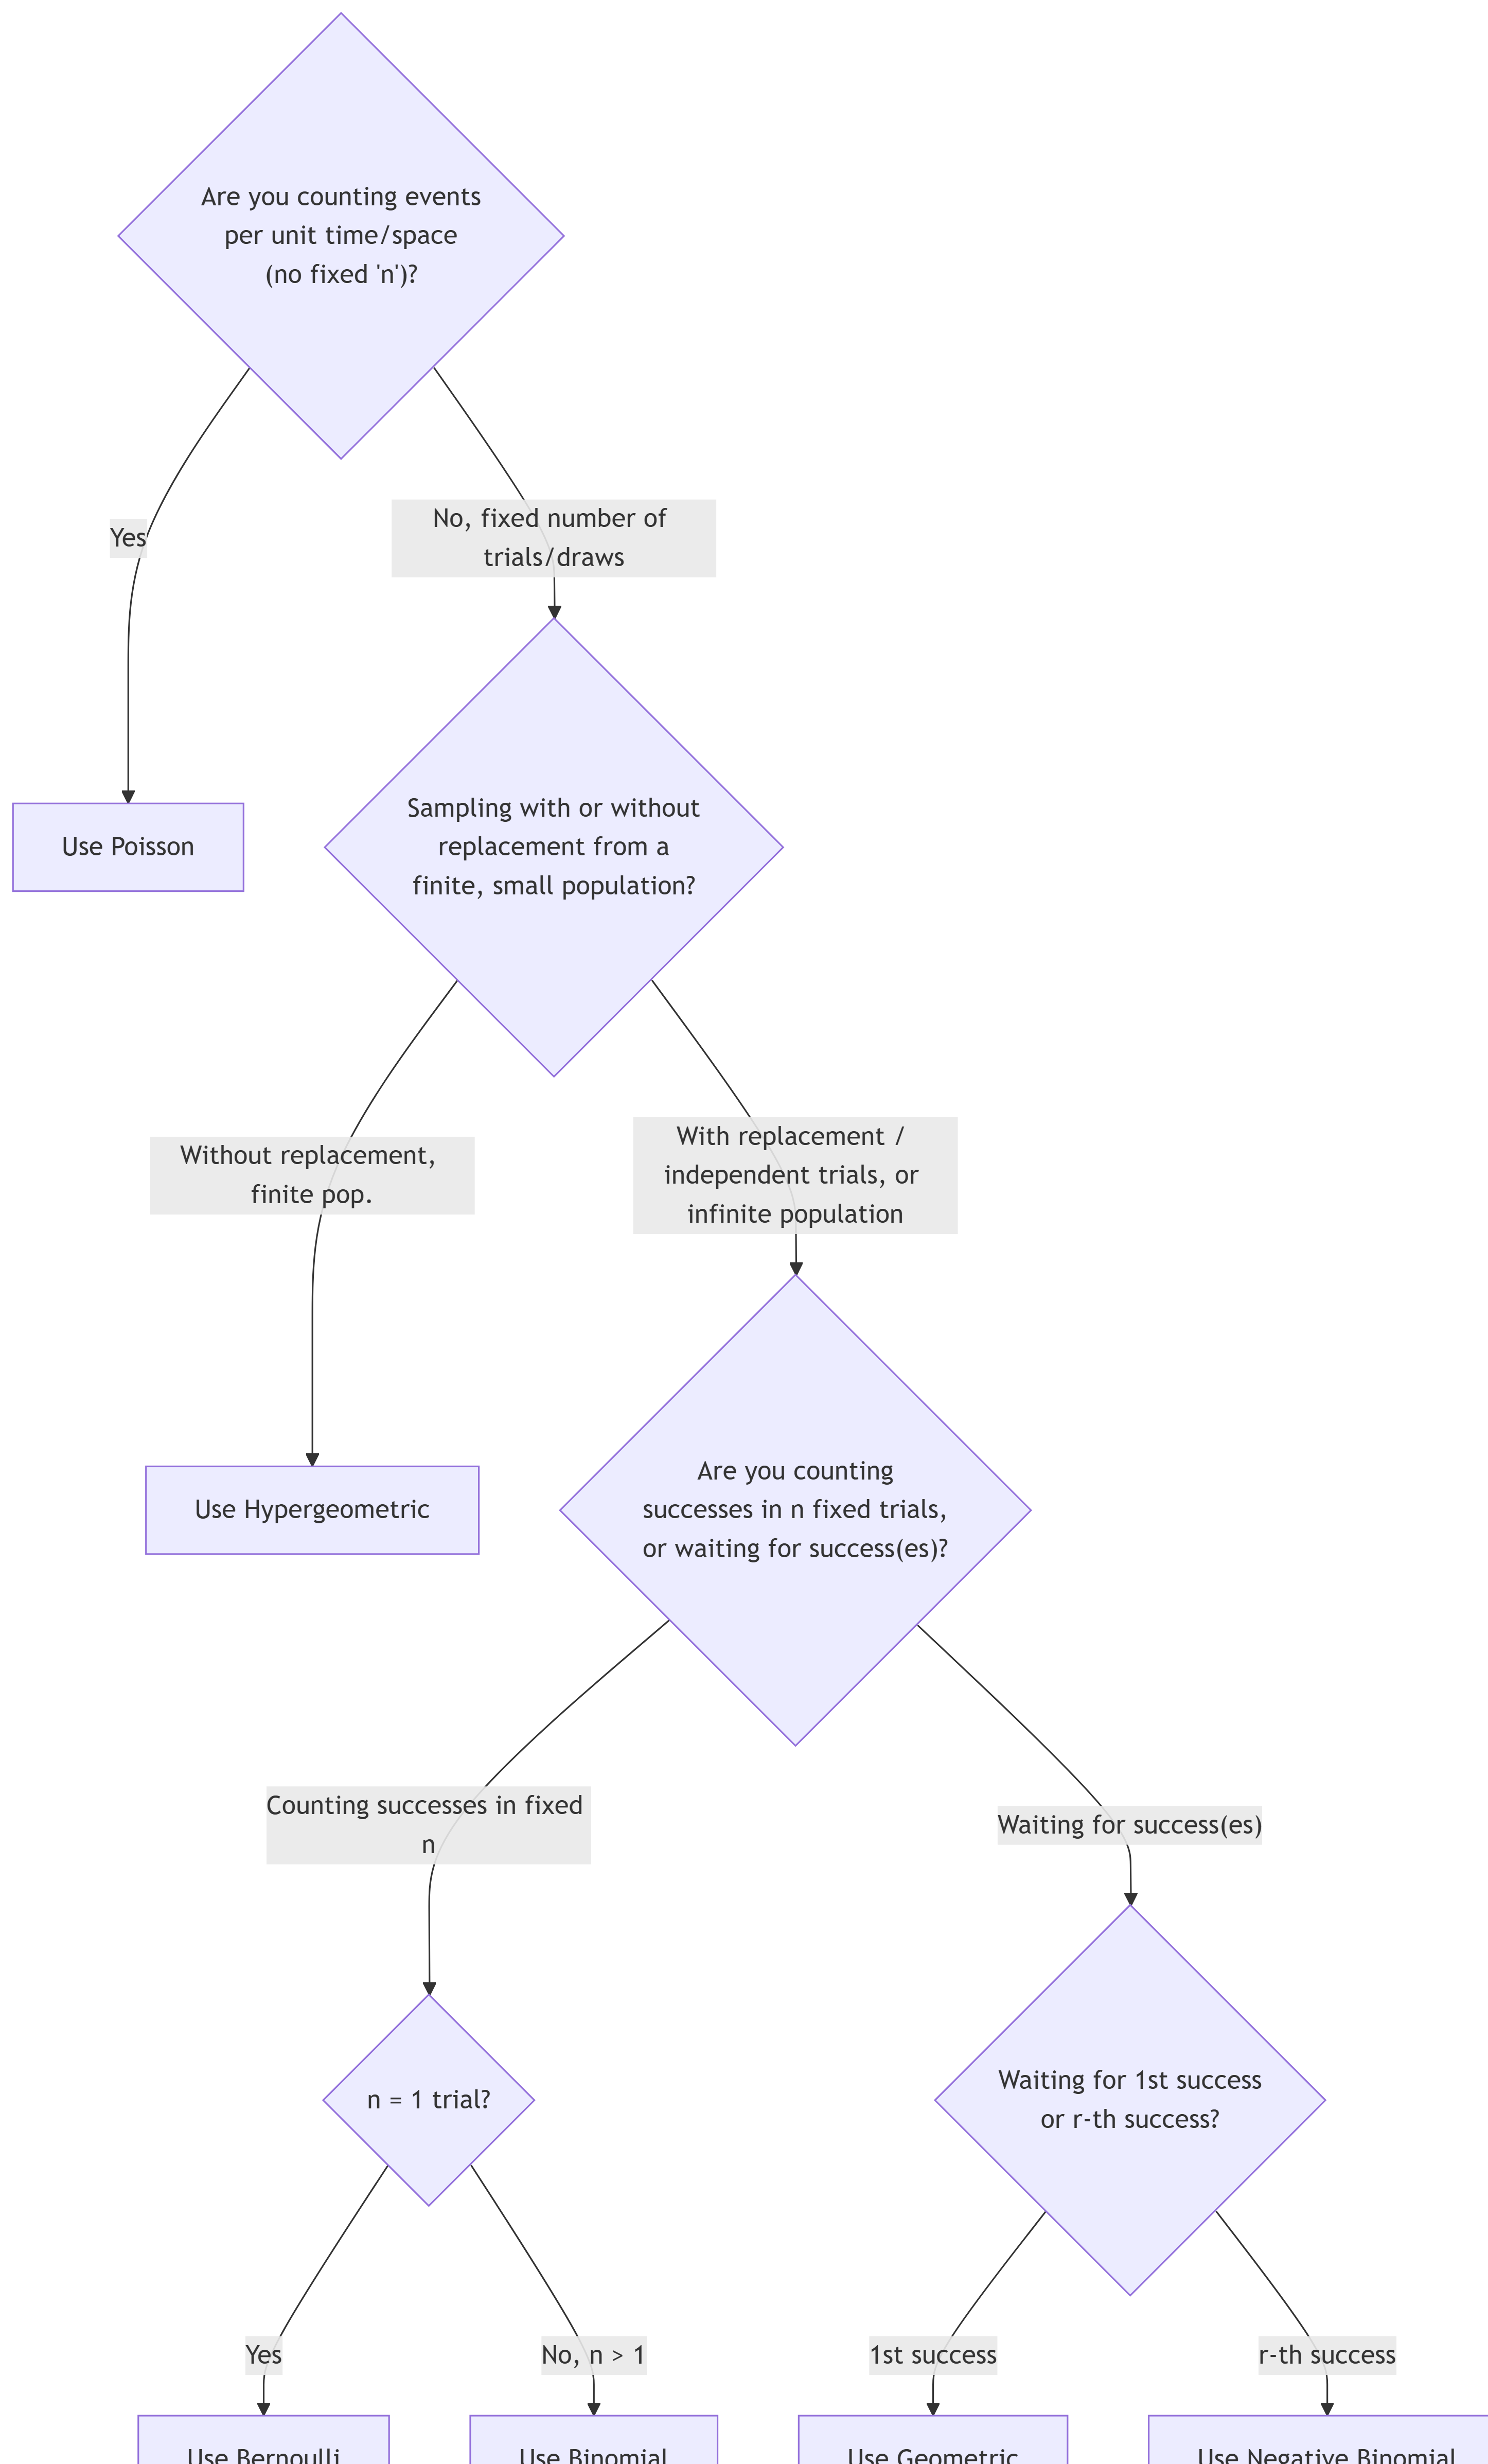
\includegraphics[width=9.75in,height=16.14in]{Section2/05_discrete_probability_distributions_files/figure-latex/mermaid-figure-1.png}

\section{Summary}\label{summary-4}

\begin{itemize}
\tightlist
\item
  A \textbf{random variable} maps outcomes of a random experiment to
  numbers; its \textbf{PMF} assigns probabilities to each possible
  value.
\item
  \textbf{Expected value} and \textbf{variance} summarize the center and
  spread of a discrete distribution.
\item
  \textbf{Bernoulli} (1 trial) generalizes to \textbf{Binomial} (\(n\)
  trials); \textbf{Geometric} (wait for 1st success) generalizes to
  \textbf{Negative Binomial} (wait for \(r\)-th success).
\item
  \textbf{Hypergeometric} is the without-replacement analogue of the
  Binomial for finite populations.
\item
  \textbf{Poisson} models rare events over a fixed interval and is the
  limiting case of the Binomial as \(n\to\infty\), \(p\to0\), with
  \(np=\lambda\) fixed.
\end{itemize}

Next section will deal with the probability distribution of
\textbf{continuous variables}.

\chapter{Continuous Probability
Distributions}\label{continuous-probability-distributions}

\section{Probability Density Function
(PDF)}\label{probability-density-function-pdf}

For a \textbf{continuous random variable}, probability is not assigned
to individual points (which each have probability zero) but to
\textbf{intervals}, via the \textbf{probability density function (PDF)},
\(f(x)\). The probability that \(X\) falls between \(a\) and \(b\) is
the area under the curve: \[P(a \le X \le b) = \int_a^b f(x)\,dx\]

A valid PDF satisfies \(f(x) \ge 0\) for all \(x\), and
\(\int_{-\infty}^{\infty} f(x)\,dx = 1\) (total area under the curve
equals 1).

\section{Cumulative Distribution Function
(CDF)}\label{cumulative-distribution-function-cdf}

\[F(x) = P(X \le x) = \int_{-\infty}^{x} f(t)\,dt\]

\(F(x)\) gives the cumulative probability up to \(x\), and is used to
find percentiles and probabilities directly.

\section{Expected Value and Variance}\label{expected-value-and-variance}

\[E(X) = \mu = \int_{-\infty}^{\infty} x f(x)\,dx \qquad Var(X) = \sigma^2 = \int_{-\infty}^{\infty}(x-\mu)^2 f(x)\,dx\]

\begin{center}\rule{0.5\linewidth}{0.5pt}\end{center}

\section{Uniform Distribution}\label{uniform-distribution}

\subsection{Definition}\label{definition-17}

All values in an interval \([a,b]\) are \textbf{equally likely}.

\subsection{PDF and CDF}\label{pdf-and-cdf}

\[f(x) = \frac{1}{b-a}, \quad a \le x \le b \qquad \]
\[F(x) = \frac{x-a}{b-a}\]

\subsection{Parameters, Mean,
Variance}\label{parameters-mean-variance-6}

\begin{longtable}[]{@{}ll@{}}
\toprule\noalign{}
Parameter & \(a\) = minimum, \(b\) = maximum \\
\midrule\noalign{}
\endhead
\bottomrule\noalign{}
\endlastfoot
Mean & \(\dfrac{a+b}{2}\) \\
Variance & \(\dfrac{(b-a)^2}{12}\) \\
\end{longtable}

\subsection{Properties}\label{properties}

Constant (flat) density; symmetric about the midpoint \((a+b)/2\).

\subsection{Applications / Public Health
Example}\label{applications-public-health-example-6}

Modeling a patient's arrival time within a clinic's operating hours as
``equally likely'' across the interval; simulation studies (uniform
random number generation is the basis for simulating other
distributions).

\subsection{Worked Example}\label{worked-example-1}

Appointment arrival times are uniformly distributed between 8:00 AM
(\(a=0\)) and 5:00 PM (\(b=9\) hours). What is the probability a patient
arrives in the first hour?
\[P(0\le X\le1) = \frac{1-0}{9-0} = 0.111 \approx 11.1\%\]

\subsection{R Code and Graph}\label{r-code-and-graph-6}

\begin{Shaded}
\begin{Highlighting}[]
\FunctionTok{ggplot}\NormalTok{(}\FunctionTok{data.frame}\NormalTok{(}\AttributeTok{x =} \FunctionTok{c}\NormalTok{(}\DecValTok{0}\NormalTok{, }\DecValTok{9}\NormalTok{)), }\FunctionTok{aes}\NormalTok{(x)) }\SpecialCharTok{+}
  \FunctionTok{stat\_function}\NormalTok{(}\AttributeTok{fun =}\NormalTok{ dunif, }\AttributeTok{args =} \FunctionTok{list}\NormalTok{(}\AttributeTok{min =} \DecValTok{0}\NormalTok{, }\AttributeTok{max =} \DecValTok{9}\NormalTok{), }\AttributeTok{geom =} \StringTok{"area"}\NormalTok{, }\AttributeTok{fill =} \StringTok{"skyblue"}\NormalTok{, }\AttributeTok{alpha =} \FloatTok{0.5}\NormalTok{) }\SpecialCharTok{+}
  \FunctionTok{labs}\NormalTok{(}\AttributeTok{title =} \StringTok{"Uniform(0, 9)"}\NormalTok{, }\AttributeTok{x =} \StringTok{"Hours after 8:00 AM"}\NormalTok{, }\AttributeTok{y =} \StringTok{"Density"}\NormalTok{) }\SpecialCharTok{+} \FunctionTok{theme\_minimal}\NormalTok{()}
\end{Highlighting}
\end{Shaded}

\begin{center}
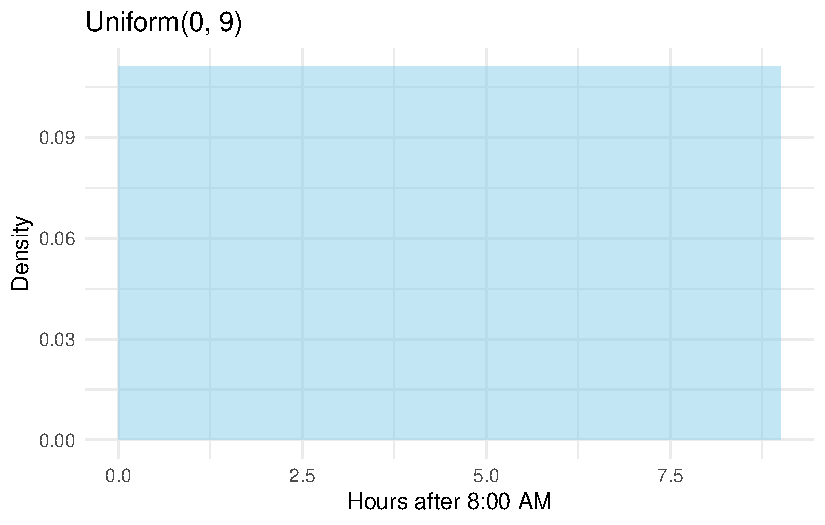
\includegraphics[width=0.85\linewidth,height=\textheight,keepaspectratio]{Section2/06_continuous_probability_distributions_files/figure-pdf/uniform-1.pdf}
\end{center}

\begin{center}\rule{0.5\linewidth}{0.5pt}\end{center}

\section{Normal (Gaussian)
Distribution}\label{normal-gaussian-distribution}

\subsection{Definition}\label{definition-18}

The most important distribution in statistics is a normal or Gaussian
distribution. It is a symmetric, bell-shaped distribution characterized
fully by its mean and standard deviation. Many biological measurements
(height, blood pressure, IQ) are approximately Normal, and the Normal
distribution is central to the Central Limit Theorem underlying most
inferential methods (Sections 9-11).

\subsection{PDF}\label{pdf}

\[f(x) = \frac{1}{\sigma\sqrt{2\pi}}\exp\left(-\frac{(x-\mu)^2}{2\sigma^2}\right), \quad -\infty<x<\infty\]

\subsection{Parameters, Mean,
Variance}\label{parameters-mean-variance-7}

\begin{longtable}[]{@{}ll@{}}
\toprule\noalign{}
Parameter & \(\mu\) = mean, \(\sigma\) = standard deviation \\
\midrule\noalign{}
\endhead
\bottomrule\noalign{}
\endlastfoot
Mean & \(\mu\) \\
Variance & \(\sigma^2\) \\
\end{longtable}

\subsection{Properties}\label{properties-1}

\begin{itemize}
\item
  Symmetric, bell-shaped, unimodal
\item
  Mean = Median = Mode.
\item
  Defined by the empirical rule:

  \begin{itemize}
  \item
    \textasciitilde68\% of values fall within \(\mu\pm1\sigma\)
  \item
    \textasciitilde95\% within \(\mu\pm2\sigma\)
  \item
    \textasciitilde99.7\% within \(\mu\pm3\sigma\)
  \end{itemize}
\item
  Notation: \(X\sim N(\mu,\sigma^2)\).
\end{itemize}

\subsection{Applications / Public Health
Example}\label{applications-public-health-example-7}

Birth weight, height, blood pressure, cholesterol levels are frequently
modeled as approximately Normal; the sampling distribution of the sample
mean is approximately Normal for large \(n\) (Central Limit Theorem),
justifying most confidence intervals and hypothesis tests in Sections 7.

\subsection{R Code and Graph}\label{r-code-and-graph-7}

\begin{Shaded}
\begin{Highlighting}[]
\FunctionTok{ggplot}\NormalTok{(}\FunctionTok{data.frame}\NormalTok{(}\AttributeTok{x =} \FunctionTok{c}\NormalTok{(}\DecValTok{40}\NormalTok{, }\DecValTok{160}\NormalTok{)), }\FunctionTok{aes}\NormalTok{(x)) }\SpecialCharTok{+}
  \FunctionTok{stat\_function}\NormalTok{(}\AttributeTok{fun =}\NormalTok{ dnorm, }\AttributeTok{args =} \FunctionTok{list}\NormalTok{(}\AttributeTok{mean =} \DecValTok{100}\NormalTok{, }\AttributeTok{sd =} \DecValTok{15}\NormalTok{), }\AttributeTok{geom =} \StringTok{"area"}\NormalTok{, }\AttributeTok{fill =} \StringTok{"tomato"}\NormalTok{, }\AttributeTok{alpha =} \FloatTok{0.5}\NormalTok{) }\SpecialCharTok{+}
  \FunctionTok{labs}\NormalTok{(}\AttributeTok{title =} \StringTok{"Normal(mean = 100, SD = 15)"}\NormalTok{, }\AttributeTok{x =} \StringTok{"X"}\NormalTok{, }\AttributeTok{y =} \StringTok{"Density"}\NormalTok{) }\SpecialCharTok{+} \FunctionTok{theme\_minimal}\NormalTok{()}
\end{Highlighting}
\end{Shaded}

\begin{center}
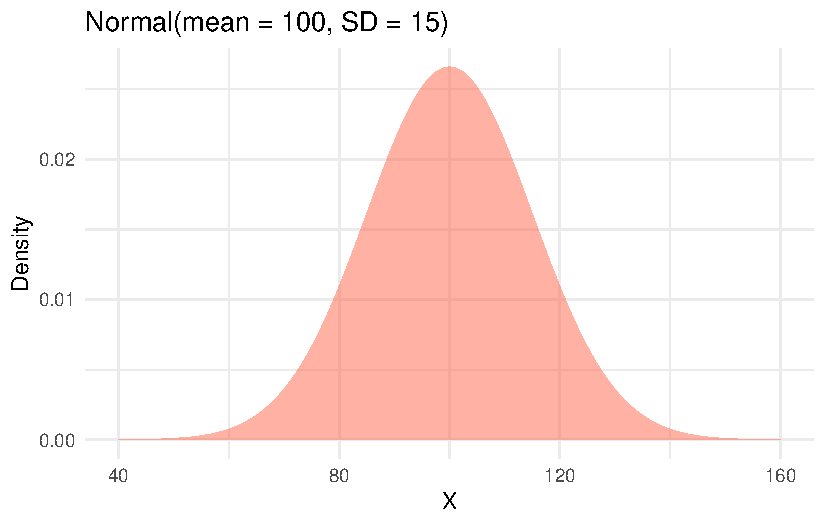
\includegraphics[width=0.85\linewidth,height=\textheight,keepaspectratio]{Section2/06_continuous_probability_distributions_files/figure-pdf/normal-1.pdf}
\end{center}

\begin{center}\rule{0.5\linewidth}{0.5pt}\end{center}

\section{Standard Normal
Distribution}\label{standard-normal-distribution}

\subsection{Definition}\label{definition-19}

The special case of the Normal distribution with \(\mu=0\) and
\(\sigma=1\), denoted \(Z \sim N(0,1)\). Any Normal variable can be
converted (``standardized'') to the standard Normal using the
\textbf{z-score}: \[Zscore = \frac{X-\mu}{\sigma}\]

\subsection{PDF}\label{pdf-1}

\[f(z) = \frac{1}{\sqrt{2\pi}}e^{-z^2/2}\]

\subsection{Worked Example (Manual
Calculation)}\label{worked-example-manual-calculation-5}

Adult male height is Normally distributed with \(\mu=170\) cm,
\(\sigma=7\) cm. What proportion of men are taller than 180 cm?

\textbf{Step 1:} Compute the z-score: \(z = \dfrac{180-170}{7} = 1.43\)

\textbf{Step 2:} Look up (or compute via software) \(P(Z>1.43)\): from
the standard Normal table, \(P(Z\le1.43)=0.9236\), so
\(P(Z>1.43) = 1-0.9236=0.0764\)

\textbf{Step 3:} Interpretation: approximately \textbf{7.6\%} of adult
men are taller than 180 cm.

\textbf{In R:} \texttt{1\ -\ pnorm(180,\ mean\ =\ 170,\ sd\ =\ 7)}
returns 0.0764.

\subsection{R Code and Graph}\label{r-code-and-graph-8}

\begin{Shaded}
\begin{Highlighting}[]
\FunctionTok{ggplot}\NormalTok{(}\FunctionTok{data.frame}\NormalTok{(}\AttributeTok{x =} \FunctionTok{c}\NormalTok{(}\SpecialCharTok{{-}}\DecValTok{4}\NormalTok{, }\DecValTok{4}\NormalTok{)), }\FunctionTok{aes}\NormalTok{(x)) }\SpecialCharTok{+}
  \FunctionTok{stat\_function}\NormalTok{(}\AttributeTok{fun =}\NormalTok{ dnorm, }\AttributeTok{geom =} \StringTok{"area"}\NormalTok{, }\AttributeTok{fill =} \StringTok{"gray70"}\NormalTok{, }\AttributeTok{alpha =} \FloatTok{0.5}\NormalTok{,}
                \AttributeTok{xlim =} \FunctionTok{c}\NormalTok{(}\FloatTok{1.43}\NormalTok{, }\DecValTok{4}\NormalTok{)) }\SpecialCharTok{+}
  \FunctionTok{stat\_function}\NormalTok{(}\AttributeTok{fun =}\NormalTok{ dnorm) }\SpecialCharTok{+}
  \FunctionTok{labs}\NormalTok{(}\AttributeTok{title =} \StringTok{"Standard Normal Z \textasciitilde{} N(0,1); shaded area = P(Z \textgreater{} 1.43)"}\NormalTok{,}
       \AttributeTok{x =} \StringTok{"z"}\NormalTok{, }\AttributeTok{y =} \StringTok{"Density"}\NormalTok{) }\SpecialCharTok{+} \FunctionTok{theme\_minimal}\NormalTok{()}
\end{Highlighting}
\end{Shaded}

\begin{center}
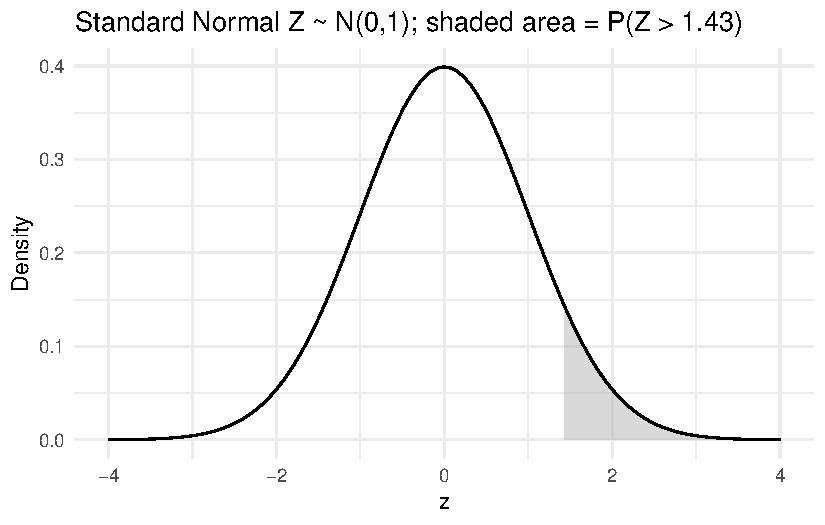
\includegraphics[width=0.85\linewidth,height=\textheight,keepaspectratio]{Section2/06_continuous_probability_distributions_files/figure-pdf/stdnormal-1.pdf}
\end{center}

\begin{center}\rule{0.5\linewidth}{0.5pt}\end{center}

\section{Exponential Distribution}\label{exponential-distribution}

\subsection{Definition}\label{definition-20}

Models the \textbf{waiting time (or distance)} until the next event in a
process where events occur at a constant average rate --- the continuous
analogue of the Geometric distribution, closely related to the Poisson
process.

\subsection{PDF and CDF}\label{pdf-and-cdf-1}

\[f(x) = \lambda e^{-\lambda x}, \quad x\ge0 \qquad F(x) = 1-e^{-\lambda x}\]

\subsection{Parameters, Mean,
Variance}\label{parameters-mean-variance-8}

\begin{longtable}[]{@{}ll@{}}
\toprule\noalign{}
Parameter & \(\lambda\) = rate parameter \\
\midrule\noalign{}
\endhead
\bottomrule\noalign{}
\endlastfoot
Mean & \(1/\lambda\) \\
Variance & \(1/\lambda^2\) \\
\end{longtable}

\subsection{Properties}\label{properties-2}

\begin{itemize}
\tightlist
\item
  Right-skewed;
\end{itemize}

\begin{itemize}
\item
  Exhibits the \textbf{memoryless property}: \(P(X>s+t\mid X>s)=P(X>t)\)

  {[}The remaining waiting time does not depend on how long you have
  already waited{]}
\end{itemize}

\subsection{Applications / Public Health
Example}\label{applications-public-health-example-8}

Time between successive patient arrivals at an emergency department;
survival time in simple constant-hazard survival models; time until
equipment failure in a medical device.

\subsection{Worked Example}\label{worked-example-2}

Patients arrive at an ED at an average rate of \(\lambda=3\) per hour.
What is the probability the next patient arrives within 10 minutes (1/6
hour)?

\textbf{Step 1:} \(F(x) = 1-e^{-\lambda x}\), with \(\lambda=3\),
\(x=1/6\)

\textbf{Step 2:} \(\lambda x = 3\times(1/6) = 0.5\)

\textbf{Step 3:}
\[P(X\le 1/6) = 1-e^{-0.5} = 1-0.6065=0.3935\approx39.4\%\]

\subsection{R Code and Graph}\label{r-code-and-graph-9}

\begin{Shaded}
\begin{Highlighting}[]
\FunctionTok{ggplot}\NormalTok{(}\FunctionTok{data.frame}\NormalTok{(}\AttributeTok{x =} \FunctionTok{c}\NormalTok{(}\DecValTok{0}\NormalTok{, }\DecValTok{2}\NormalTok{)), }\FunctionTok{aes}\NormalTok{(x)) }\SpecialCharTok{+}
  \FunctionTok{stat\_function}\NormalTok{(}\AttributeTok{fun =}\NormalTok{ dexp, }\AttributeTok{args =} \FunctionTok{list}\NormalTok{(}\AttributeTok{rate =} \DecValTok{3}\NormalTok{), }\AttributeTok{geom =} \StringTok{"area"}\NormalTok{, }\AttributeTok{fill =} \StringTok{"darkgreen"}\NormalTok{, }\AttributeTok{alpha =} \FloatTok{0.5}\NormalTok{) }\SpecialCharTok{+}
  \FunctionTok{labs}\NormalTok{(}\AttributeTok{title =} \StringTok{"Exponential(rate = 3 per hour)"}\NormalTok{, }\AttributeTok{x =} \StringTok{"Hours until next arrival"}\NormalTok{, }\AttributeTok{y =} \StringTok{"Density"}\NormalTok{) }\SpecialCharTok{+} \FunctionTok{theme\_minimal}\NormalTok{()}
\end{Highlighting}
\end{Shaded}

\begin{center}
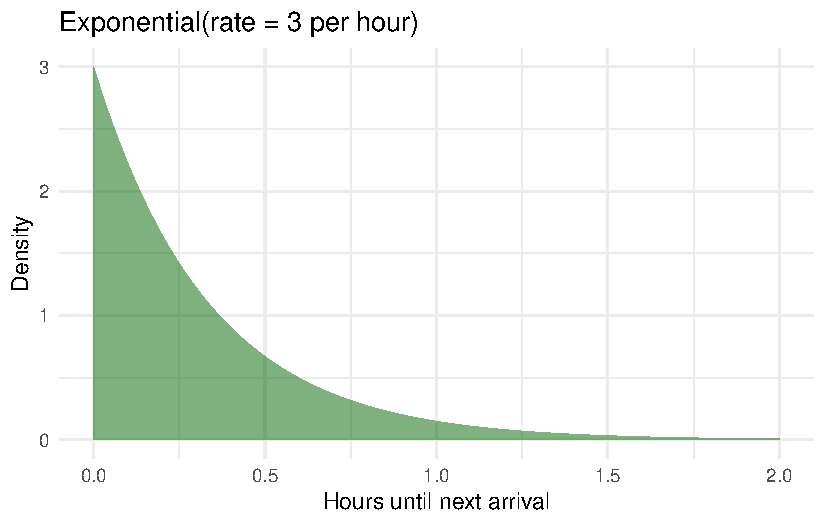
\includegraphics[width=0.85\linewidth,height=\textheight,keepaspectratio]{Section2/06_continuous_probability_distributions_files/figure-pdf/exponential-1.pdf}
\end{center}

\begin{center}\rule{0.5\linewidth}{0.5pt}\end{center}

\section{Gamma Distribution}\label{gamma-distribution}

\subsection{Definition}\label{definition-21}

Generalizes the Exponential distribution to model the \textbf{waiting
time until the} \(k\)-th event in a Poisson process (analogous to how
Negative Binomial generalizes Geometric in the discrete case).

\subsection{PDF}\label{pdf-2}

\[f(x) = \frac{\lambda^k x^{k-1}e^{-\lambda x}}{\Gamma(k)}, \quad x>0\]
where \(\Gamma(k)\) is the Gamma function (for integer \(k\),
\(\Gamma(k)=(k-1)!\)).

\subsection{Parameters, Mean,
Variance}\label{parameters-mean-variance-9}

\begin{longtable}[]{@{}ll@{}}
\toprule\noalign{}
Parameter & \(k\) (shape), \(\lambda\) (rate) \\
\midrule\noalign{}
\endhead
\bottomrule\noalign{}
\endlastfoot
Mean & \(k/\lambda\) \\
Variance & \(k/\lambda^2\) \\
\end{longtable}

\subsection{Properties}\label{properties-3}

\begin{itemize}
\item
  Right-skewed for small \(k\), approaching Normal shape as \(k\)
  increases
\item
  Exponential distribution is the special case at \(k=1\)
\item
  Chi-square distribution (below) is also a special case of the Gamma.
\end{itemize}

\subsection{Applications / Public Health
Example}\label{applications-public-health-example-9}

Modeling time until \(k\) disease relapses occur; modeling right-skewed
cost or length-of-stay data in health economics; modeling total rainfall
or time until \(k\)-th case in an outbreak.

\subsection{R Code and Graph}\label{r-code-and-graph-10}

\begin{Shaded}
\begin{Highlighting}[]
\FunctionTok{ggplot}\NormalTok{(}\FunctionTok{data.frame}\NormalTok{(}\AttributeTok{x =} \FunctionTok{c}\NormalTok{(}\DecValTok{0}\NormalTok{, }\DecValTok{10}\NormalTok{)), }\FunctionTok{aes}\NormalTok{(x)) }\SpecialCharTok{+}
  \FunctionTok{stat\_function}\NormalTok{(}\AttributeTok{fun =}\NormalTok{ dgamma, }\AttributeTok{args =} \FunctionTok{list}\NormalTok{(}\AttributeTok{shape =} \DecValTok{3}\NormalTok{, }\AttributeTok{rate =} \DecValTok{1}\NormalTok{), }\AttributeTok{geom =} \StringTok{"area"}\NormalTok{, }\AttributeTok{fill =} \StringTok{"orchid"}\NormalTok{, }\AttributeTok{alpha =} \FloatTok{0.5}\NormalTok{) }\SpecialCharTok{+}
  \FunctionTok{labs}\NormalTok{(}\AttributeTok{title =} \StringTok{"Gamma(shape = 3, rate = 1)"}\NormalTok{, }\AttributeTok{x =} \StringTok{"X"}\NormalTok{, }\AttributeTok{y =} \StringTok{"Density"}\NormalTok{) }\SpecialCharTok{+} \FunctionTok{theme\_minimal}\NormalTok{()}
\end{Highlighting}
\end{Shaded}

\begin{center}
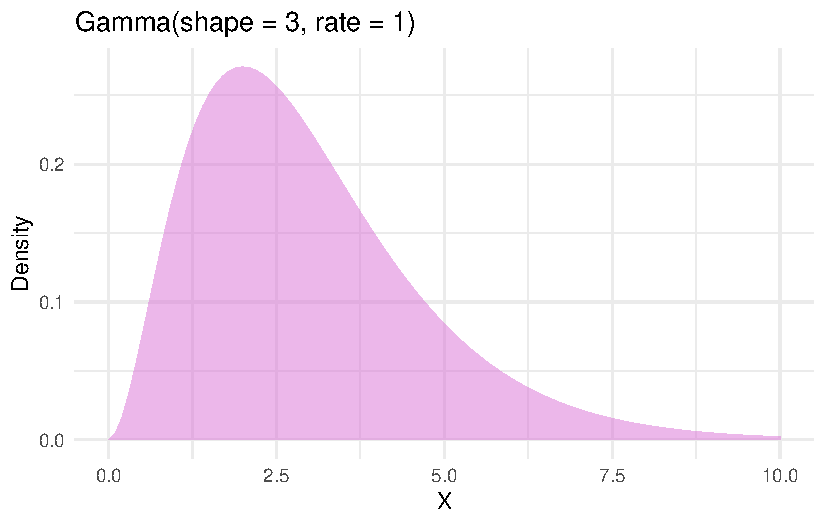
\includegraphics[width=0.85\linewidth,height=\textheight,keepaspectratio]{Section2/06_continuous_probability_distributions_files/figure-pdf/gamma-1.pdf}
\end{center}

\begin{center}\rule{0.5\linewidth}{0.5pt}\end{center}

\section{Chi-Square Distribution}\label{chi-square-distribution}

\subsection{Definition}\label{definition-22}

The distribution of the \textbf{sum of squares of} \(k\) independent
standard Normal variables; a special case of the Gamma distribution
(\(k\) degrees of freedom, rate \(=1/2\)). Central to goodness-of-fit
tests, tests of independence in contingency tables, and the sampling
distribution of the sample variance.

\[X = \sum_{i=1}^{k} Z_i^2 \sim \chi^2_k\]

\subsection{Parameters, Mean,
Variance}\label{parameters-mean-variance-10}

\begin{longtable}[]{@{}ll@{}}
\toprule\noalign{}
Parameter & \(k\) = degrees of freedom \\
\midrule\noalign{}
\endhead
\bottomrule\noalign{}
\endlastfoot
Mean & \(k\) \\
Variance & \(2k\) \\
\end{longtable}

\subsection{Properties}\label{properties-4}

\begin{itemize}
\item
  Right-skewed, especially for small \(k\)
\item
  Becomes more symmetric (approaching Normal) as \(k\) increases
\item
  Always non-negative.
\end{itemize}

\subsection{Applications / Public Health
Example}\label{applications-public-health-example-10}

Chi-square test of independence for contingency tables (e.g., testing
association between vaccination status and infection outcome);
goodness-of-fit tests; constructing confidence intervals for a
population variance.

\subsection{R Code and Graph}\label{r-code-and-graph-11}

\begin{Shaded}
\begin{Highlighting}[]
\FunctionTok{ggplot}\NormalTok{(}\FunctionTok{data.frame}\NormalTok{(}\AttributeTok{x =} \FunctionTok{c}\NormalTok{(}\DecValTok{0}\NormalTok{, }\DecValTok{20}\NormalTok{)), }\FunctionTok{aes}\NormalTok{(x)) }\SpecialCharTok{+}
  \FunctionTok{stat\_function}\NormalTok{(}\AttributeTok{fun =}\NormalTok{ dchisq, }\AttributeTok{args =} \FunctionTok{list}\NormalTok{(}\AttributeTok{df =} \DecValTok{4}\NormalTok{), }\AttributeTok{geom =} \StringTok{"area"}\NormalTok{, }\AttributeTok{fill =} \StringTok{"chocolate"}\NormalTok{, }\AttributeTok{alpha =} \FloatTok{0.5}\NormalTok{) }\SpecialCharTok{+}
  \FunctionTok{labs}\NormalTok{(}\AttributeTok{title =} \StringTok{"Chi{-}square(df = 4)"}\NormalTok{, }\AttributeTok{x =} \StringTok{"X"}\NormalTok{, }\AttributeTok{y =} \StringTok{"Density"}\NormalTok{) }\SpecialCharTok{+} \FunctionTok{theme\_minimal}\NormalTok{()}
\end{Highlighting}
\end{Shaded}

\begin{center}
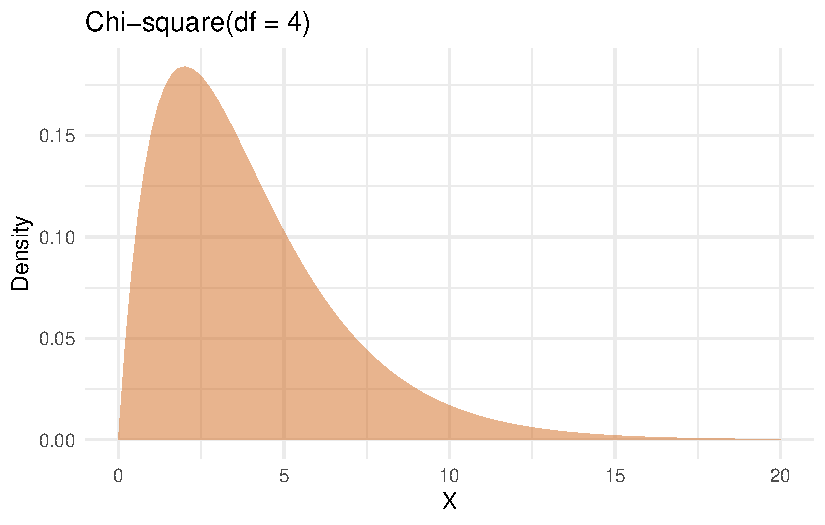
\includegraphics[width=0.85\linewidth,height=\textheight,keepaspectratio]{Section2/06_continuous_probability_distributions_files/figure-pdf/chisq-1.pdf}
\end{center}

\begin{center}\rule{0.5\linewidth}{0.5pt}\end{center}

\section{Student's t-Distribution}\label{students-t-distribution}

\subsection{Definition}\label{definition-23}

Similar in shape to the standard Normal, but with \textbf{heavier
tails}, used when estimating a population mean with an \textbf{unknown
population variance} and a small sample size (the sample SD, \(s\), is
used in place of \(\sigma\)).

\[t = \frac{\bar{x}-\mu}{s/\sqrt{n}} \sim t_{n-1}\]

\subsection{Parameters, Mean,
Variance}\label{parameters-mean-variance-11}

\begin{longtable}[]{@{}ll@{}}
\toprule\noalign{}
Parameter & \(\nu\) (degrees of freedom, typically \(n-1\)) \\
\midrule\noalign{}
\endhead
\bottomrule\noalign{}
\endlastfoot
Mean & \(0\) (for \(\nu>1\)) \\
Variance & \(\dfrac{\nu}{\nu-2}\) (for \(\nu>2\)) \\
\end{longtable}

\subsection{Properties}\label{properties-5}

\begin{itemize}
\item
  Symmetric, bell-shaped, centered at 0
\item
  Heavier tails than the standard Normal, especially for small \(\nu\);
  converges to the standard Normal as \(\nu\to\infty\) (in practice,
  \(t\) and \(Z\) are nearly identical for \(\nu>30\)).
\end{itemize}

\subsection{Applications / Public Health
Example}\label{applications-public-health-example-11}

The basis for the \textbf{one-sample and two-sample t-tests} and t-based
confidence intervals for means (used throughout later chapters) when
sample sizes are small and population SD is unknown, the standard
situation in most clinical studies.

\subsection{R Code and Graph}\label{r-code-and-graph-12}

\begin{Shaded}
\begin{Highlighting}[]
\FunctionTok{ggplot}\NormalTok{(}\FunctionTok{data.frame}\NormalTok{(}\AttributeTok{x =} \FunctionTok{c}\NormalTok{(}\SpecialCharTok{{-}}\DecValTok{4}\NormalTok{, }\DecValTok{4}\NormalTok{)), }\FunctionTok{aes}\NormalTok{(x)) }\SpecialCharTok{+}
  \FunctionTok{stat\_function}\NormalTok{(}\AttributeTok{fun =}\NormalTok{ dt, }\AttributeTok{args =} \FunctionTok{list}\NormalTok{(}\AttributeTok{df =} \DecValTok{5}\NormalTok{), }\FunctionTok{aes}\NormalTok{(}\AttributeTok{color =} \StringTok{"t (df=5)"}\NormalTok{)) }\SpecialCharTok{+}
  \FunctionTok{stat\_function}\NormalTok{(}\AttributeTok{fun =}\NormalTok{ dnorm, }\FunctionTok{aes}\NormalTok{(}\AttributeTok{color =} \StringTok{"Standard Normal"}\NormalTok{)) }\SpecialCharTok{+}
  \FunctionTok{labs}\NormalTok{(}\AttributeTok{title =} \StringTok{"Student\textquotesingle{}s t (df = 5) vs Standard Normal"}\NormalTok{, }\AttributeTok{x =} \StringTok{"x"}\NormalTok{, }\AttributeTok{y =} \StringTok{"Density"}\NormalTok{, }\AttributeTok{color =} \StringTok{""}\NormalTok{) }\SpecialCharTok{+}
  \FunctionTok{theme\_minimal}\NormalTok{()}
\end{Highlighting}
\end{Shaded}

\begin{center}
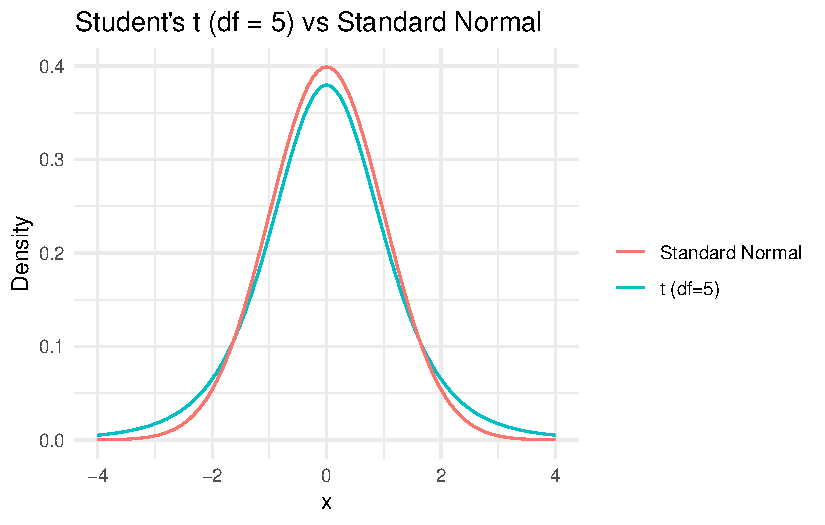
\includegraphics[width=0.85\linewidth,height=\textheight,keepaspectratio]{Section2/06_continuous_probability_distributions_files/figure-pdf/tdist-1.pdf}
\end{center}

\begin{center}\rule{0.5\linewidth}{0.5pt}\end{center}

\section{F Distribution}\label{f-distribution}

\subsection{Definition}\label{definition-24}

The distribution of the \textbf{ratio of two independent chi-square
variables}, each divided by their own degrees of freedom, used to
compare two variances, and as the basis for ANOVA (Analysis of
Variance).

\[F = \frac{\chi^2_{d_1}/d_1}{\chi^2_{d_2}/d_2} \sim F_{d_1,d_2}\]

\subsection{Parameters, Mean,
Variance}\label{parameters-mean-variance-12}

\begin{longtable}[]{@{}
  >{\raggedright\arraybackslash}p{(\linewidth - 2\tabcolsep) * \real{0.1571}}
  >{\raggedright\arraybackslash}p{(\linewidth - 2\tabcolsep) * \real{0.8429}}@{}}
\toprule\noalign{}
\begin{minipage}[b]{\linewidth}\raggedright
Parameter
\end{minipage} & \begin{minipage}[b]{\linewidth}\raggedright
\(d_1\) (numerator df), \(d_2\) (denominator df)
\end{minipage} \\
\midrule\noalign{}
\endhead
\bottomrule\noalign{}
\endlastfoot
Mean & \(\dfrac{d_2}{d_2-2}\) (for \(d_2>2\)) \\
Variance & Complex expression involving both \(d_1,d_2\) (for
\(d_2>4\)) \\
\end{longtable}

\subsection{Properties}\label{properties-6}

Right-skewed, always non-negative; shape depends on both degrees of
freedom; approaches Normal-like shape as both \(d_1,d_2\) grow large.

\subsection{Applications / Public Health
Example}\label{applications-public-health-example-12}

Comparing variability between two treatment groups (F-test for equal
variances); the basis of \textbf{ANOVA}, used to compare means across
three or more groups (e.g., comparing mean recovery time across three
treatment protocols).

\subsection{R Code and Graph}\label{r-code-and-graph-13}

\begin{Shaded}
\begin{Highlighting}[]
\FunctionTok{ggplot}\NormalTok{(}\FunctionTok{data.frame}\NormalTok{(}\AttributeTok{x =} \FunctionTok{c}\NormalTok{(}\DecValTok{0}\NormalTok{, }\DecValTok{5}\NormalTok{)), }\FunctionTok{aes}\NormalTok{(x)) }\SpecialCharTok{+}
  \FunctionTok{stat\_function}\NormalTok{(}\AttributeTok{fun =}\NormalTok{ df, }\AttributeTok{args =} \FunctionTok{list}\NormalTok{(}\AttributeTok{df1 =} \DecValTok{5}\NormalTok{, }\AttributeTok{df2 =} \DecValTok{20}\NormalTok{), }\AttributeTok{geom =} \StringTok{"area"}\NormalTok{, }\AttributeTok{fill =} \StringTok{"gold"}\NormalTok{, }\AttributeTok{alpha =} \FloatTok{0.5}\NormalTok{) }\SpecialCharTok{+}
  \FunctionTok{labs}\NormalTok{(}\AttributeTok{title =} \StringTok{"F(df1 = 5, df2 = 20)"}\NormalTok{, }\AttributeTok{x =} \StringTok{"F"}\NormalTok{, }\AttributeTok{y =} \StringTok{"Density"}\NormalTok{) }\SpecialCharTok{+} \FunctionTok{theme\_minimal}\NormalTok{()}
\end{Highlighting}
\end{Shaded}

\begin{center}
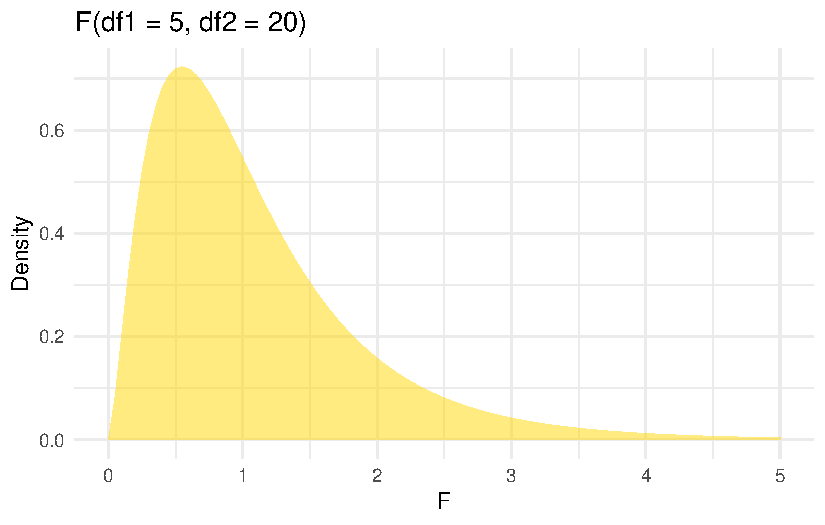
\includegraphics[width=0.85\linewidth,height=\textheight,keepaspectratio]{Section2/06_continuous_probability_distributions_files/figure-pdf/fdist-1.pdf}
\end{center}

\begin{center}\rule{0.5\linewidth}{0.5pt}\end{center}

\section{Comparison Table --- Continuous
Distributions}\label{comparison-table-continuous-distributions}

\begin{longtable}[]{@{}
  >{\raggedright\arraybackslash}p{(\linewidth - 12\tabcolsep) * \real{0.1429}}
  >{\raggedright\arraybackslash}p{(\linewidth - 12\tabcolsep) * \real{0.1429}}
  >{\raggedright\arraybackslash}p{(\linewidth - 12\tabcolsep) * \real{0.1429}}
  >{\raggedright\arraybackslash}p{(\linewidth - 12\tabcolsep) * \real{0.1429}}
  >{\raggedright\arraybackslash}p{(\linewidth - 12\tabcolsep) * \real{0.1429}}
  >{\raggedright\arraybackslash}p{(\linewidth - 12\tabcolsep) * \real{0.1429}}
  >{\raggedright\arraybackslash}p{(\linewidth - 12\tabcolsep) * \real{0.1429}}@{}}
\toprule\noalign{}
\begin{minipage}[b]{\linewidth}\raggedright
Distribution
\end{minipage} & \begin{minipage}[b]{\linewidth}\raggedright
Range
\end{minipage} & \begin{minipage}[b]{\linewidth}\raggedright
Parameters
\end{minipage} & \begin{minipage}[b]{\linewidth}\raggedright
Mean
\end{minipage} & \begin{minipage}[b]{\linewidth}\raggedright
Variance
\end{minipage} & \begin{minipage}[b]{\linewidth}\raggedright
Shape
\end{minipage} & \begin{minipage}[b]{\linewidth}\raggedright
Typical Use
\end{minipage} \\
\midrule\noalign{}
\endhead
\bottomrule\noalign{}
\endlastfoot
Uniform & \([a,b]\) & \(a, b\) & \((a+b)/2\) & \((b-a)^2/12\) & Flat &
Equally likely outcomes \\
Normal & \((-\infty,\infty)\) & \(\mu,\sigma\) & \(\mu\) & \(\sigma^2\)
& Symmetric, bell & Biological measurements, CLT \\
Standard Normal & \((-\infty,\infty)\) & none (\(\mu=0,\sigma=1\)) & 0 &
1 & Symmetric, bell & z-scores, standardization \\
Exponential & \([0,\infty)\) & \(\lambda\) & \(1/\lambda\) &
\(1/\lambda^2\) & Right-skewed & Waiting times, survival \\
Gamma & \([0,\infty)\) & \(k,\lambda\) & \(k/\lambda\) & \(k/\lambda^2\)
& Right-skewed & Time to \(k\)-th event, cost data \\
Chi-square & \([0,\infty)\) & \(k\) (df) & \(k\) & \(2k\) & Right-skewed
& Variance tests, goodness-of-fit \\
Student's t & \((-\infty,\infty)\) & \(\nu\) (df) & 0 & \(\nu/(\nu-2)\)
& Symmetric, heavy tails & Small-sample mean inference \\
F & \([0,\infty)\) & \(d_1,d_2\) (df) & \(d_2/(d_2-2)\) & complex &
Right-skewed & ANOVA, variance ratio tests \\
\end{longtable}

\section{Decision Guide: Which Continuous Distribution Should I
Use?}\label{decision-guide-which-continuous-distribution-should-i-use}

\begin{Shaded}
\begin{Highlighting}[]
\NormalTok{flowchart TD}
\NormalTok{    Q1\{"What are you modeling?"\} {-}{-}\textgreater{} Q2["A single continuous\textless{}br/\textgreater{}measurement, symmetric,\textless{}br/\textgreater{}bell{-}shaped?"]}
\NormalTok{    Q1 {-}{-}\textgreater{} Q3["Waiting time / time{-}to{-}event?"]}
\NormalTok{    Q1 {-}{-}\textgreater{} Q4["A test statistic for\textless{}br/\textgreater{}inference?"]}
\NormalTok{    Q1 {-}{-}\textgreater{} Q5["All outcomes\textless{}br/\textgreater{}equally likely in a range?"]}
\NormalTok{    Q2 {-}{-}\textgreater{}|Yes| Normal["Use Normal\textless{}br/\textgreater{}(or Standard Normal if standardized)"]}
\NormalTok{    Q3 {-}{-}\textgreater{}|"Time to 1st event"| Expo["Use Exponential"]}
\NormalTok{    Q3 {-}{-}\textgreater{}|"Time to k{-}th event"| Gam["Use Gamma"]}
\NormalTok{    Q5 {-}{-}\textgreater{}|Yes| Unif["Use Uniform"]}
\NormalTok{    Q4 {-}{-}\textgreater{} Q6\{"Comparing a mean,\textless{}br/\textgreater{}small n, sigma unknown?"\}}
\NormalTok{    Q4 {-}{-}\textgreater{} Q7\{"Testing a variance or\textless{}br/\textgreater{}categorical association?"\}}
\NormalTok{    Q4 {-}{-}\textgreater{} Q8\{"Comparing variances\textless{}br/\textgreater{}across 3+ groups (ANOVA)?"\}}
\NormalTok{    Q6 {-}{-}\textgreater{}|Yes| Tdist["Use Student\textquotesingle{}s t"]}
\NormalTok{    Q7 {-}{-}\textgreater{}|Yes| Chisq["Use Chi{-}square"]}
\NormalTok{    Q8 {-}{-}\textgreater{}|Yes| Fdist["Use F distribution"]}
\end{Highlighting}
\end{Shaded}

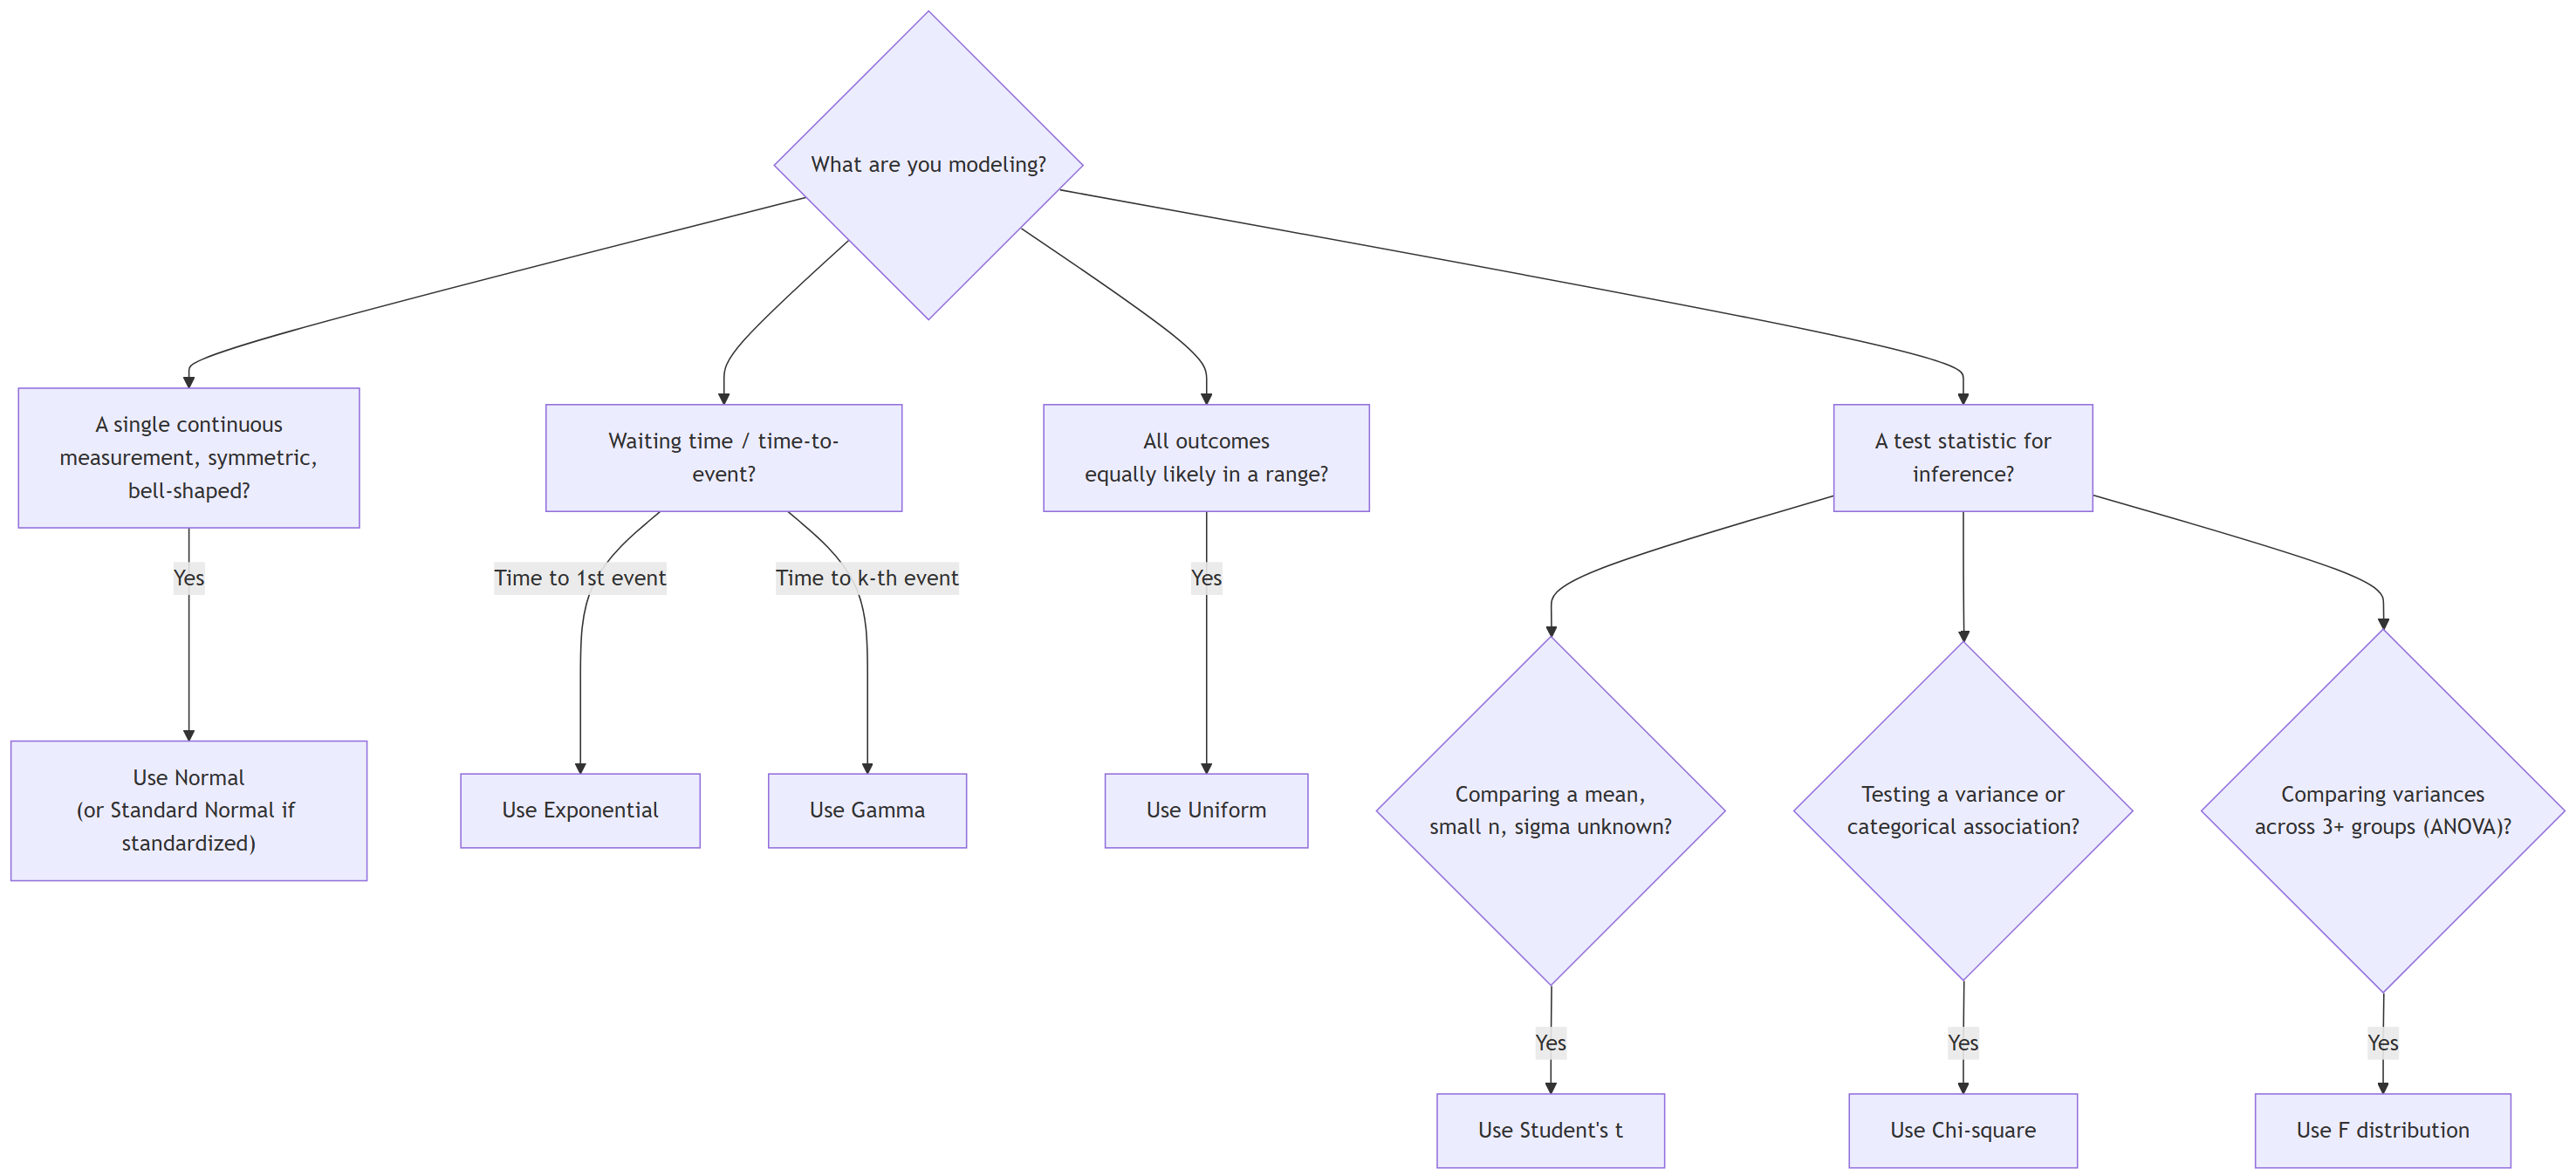
\includegraphics[width=19.6in,height=8.97in]{Section2/06_continuous_probability_distributions_files/figure-latex/mermaid-figure-1.png}

\section{Summary}\label{summary-5}

\begin{itemize}
\tightlist
\item
  Continuous distributions use a \textbf{PDF} (density, area =
  probability) and \textbf{CDF} (cumulative probability) rather than a
  PMF.
\item
  The \textbf{Normal distribution} is central to biostatistics because
  of the Central Limit Theorem; the \textbf{Standard Normal} enables
  z-score based probability calculations.
\item
  The \textbf{Exponential} and \textbf{Gamma} distributions model
  waiting times, closely paralleling the discrete Geometric and Negative
  Binomial distributions.
\item
  The \textbf{Chi-square}, \textbf{Student's t}, and \textbf{F
  distributions} are not typically used to model raw data directly ---
  they arise as \textbf{sampling distributions of test statistics}, and
  are the foundation of the hypothesis testing methods introduced in
  Sections 9-11 and developed throughout the rest of this book.
\end{itemize}

Sections 9-11 now turn from probability theory to \textbf{statistical
inference}: using these distributions to test hypotheses and estimate
population parameters from sample data.

\chapter{Hypothesis Testing}\label{hypothesis-testing}

\chapter{Introduction}\label{introduction-4}

Having established descriptive statistics and probability distributions,
we now turn to \textbf{inferential statistics}. It is used to draw
conclusions about a population from sample data. \textbf{Hypothesis
testing} is a formal procedure for deciding whether sample data provide
enough evidence to support a claim about a population.

\section{Population Parameter vs.~Sample
Statistic}\label{population-parameter-vs.-sample-statistic}

As introduced in Chapter 1, a \textbf{population parameter} (e.g.,
\(\mu\), \(\sigma\), \(\pi\)) is a fixed, usually unknown, numerical
characteristic of an entire population. A \textbf{sample statistic}
(e.g., \(\bar{x}\), \(s\), \(\hat{p}\)) is computed from sample data and
used to estimate the corresponding parameter. Hypothesis testing uses
sample statistic, together with its known sampling distribution, to make
a probabilistic statement about the population parameter.

\section{Research Hypothesis, Null, and Alternative
Hypothesis}\label{research-hypothesis-null-and-alternative-hypothesis}

\begin{itemize}
\item
  \textbf{Research hypothesis:} The substantive question or claim the
  investigator wants to evaluate (e.g., ``a new antihypertensive drug
  lowers blood pressure more than the standard drug'').
\item
  \textbf{Null hypothesis (}\(H_0\)): A statement of ``no effect,'' ``no
  difference,'' or ``no association'' .It is the default position that
  is assumed true until evidence suggests otherwise.

  Example: \(H_0: \mu_{new}=\mu_{standard}\).
\item
  \textbf{Alternative hypothesis (}\(H_1\) or \(H_a\)): The statement
  that contradicts \(H_0\), representing what the researcher suspects
  may actually be true.

  Example: \(H_a: \mu_{new} \ne \mu_{standard}\) (or \(<\), or \(>\),
  depending on the research question).
\end{itemize}

\begin{tcolorbox}[enhanced jigsaw, bottomrule=.15mm, breakable, opacityback=0, toptitle=1mm, titlerule=0mm, bottomtitle=1mm, colback=white, arc=.35mm, rightrule=.15mm, toprule=.15mm, leftrule=.75mm, title=\textcolor{quarto-callout-note-color}{\faInfo}\hspace{0.5em}{Note}, colbacktitle=quarto-callout-note-color!10!white, colframe=quarto-callout-note-color-frame, coltitle=black, left=2mm, opacitybacktitle=0.6]

Hypothesis testing follows the logic of a courtroom trial: \(H_0\)
(``the defendant is innocent'') is assumed true until the evidence
(data) is strong enough to reject it ``beyond reasonable doubt'' (a
pre-specified significance level) in favor of \(H_a\) (``the defendant
is guilty''). We never ``prove'' \(H_0\) true; we only fail to reject
it, or reject it in favor of \(H_a\).

\end{tcolorbox}

\section{\texorpdfstring{Significance Level
(\(\alpha\))}{Significance Level (\textbackslash alpha)}}\label{significance-level-alpha}

The \textbf{significance level}, \(\alpha\), is the threshold
probability of incorrectly rejecting a true null hypothesis (a
\textbf{Type I error}, detailed in Section 10) that the researcher is
willing to accept, chosen \textbf{before} collecting/analyzing data.
Common conventions: \(\alpha=0.05\) (5\%), \(\alpha=0.01\) (1\%).

\section{Test Statistic}\label{test-statistic}

A \textbf{test statistic} is a single value, computed from the sample
data, that measures how far the observed data deviate from what would be
expected under \(H_0\). Its form depends on the hypothesis and data type
(e.g., \(z\), \(t\), \(\chi^2\), \(F\) ).

General structure of test statistics is as follows:
\[\text{Test statistic} = \frac{\text{Observed estimate} - \text{Hypothesized value under } H_0}{\text{Standard error of the estimate}}\]

\section{P-value}\label{p-value}

The \textbf{p-value} is the probability of obtaining a test statistic
\textbf{as extreme as, or more extreme than}, the one observed,
\textbf{assuming} \(H_0\) is true. A small p-value indicates the
observed data would be unusual if \(H_0\) were true, providing evidence
against \(H_0\).

\begin{tcolorbox}[enhanced jigsaw, bottomrule=.15mm, breakable, opacityback=0, toptitle=1mm, titlerule=0mm, bottomtitle=1mm, colback=white, arc=.35mm, rightrule=.15mm, toprule=.15mm, leftrule=.75mm, title=\textcolor{quarto-callout-important-color}{\faExclamation}\hspace{0.5em}{Important}, colbacktitle=quarto-callout-important-color!10!white, colframe=quarto-callout-important-color-frame, coltitle=black, left=2mm, opacitybacktitle=0.6]

A p-value is \textbf{not} the probability that \(H_0\) is true, and it
is \textbf{not} the probability the results occurred ``by chance'' in a
broad sense. It is a conditional probability:
\(P(\text{data this extreme or more} \mid H_0 \text{ true})\).
Misinterpreting the p-value is one of the most common errors in the
interpretation of statistical results.

\end{tcolorbox}

\section{Critical Value and Decision
Rule}\label{critical-value-and-decision-rule}

The \textbf{critical value} is the cutoff value of the test statistic
that separates the ``rejection region'' from the ``non-rejection
region,'' determined by \(\alpha\) and the sampling distribution of the
test statistic.

Decision for a hypothesis can be taken using two approaches. First
decision rule is based on p-value \textbf{(p-value approach)}. In this
approach, null hypothesis (\(H_0\)) is rejected if p-value
\(\le \alpha\), and otherwise failed to reject null hypothesis
(\(H_0\)). Second decison rule is based on critical value
\textbf{(critical value approach).} In this appraoch, \(H_0\) is
rejected if the test statistic falls in the rejection region (beyond the
critical value), and otherwise, fail to reject \(H_0\).

Both approaches always give the same conclusion for a given \(\alpha\).

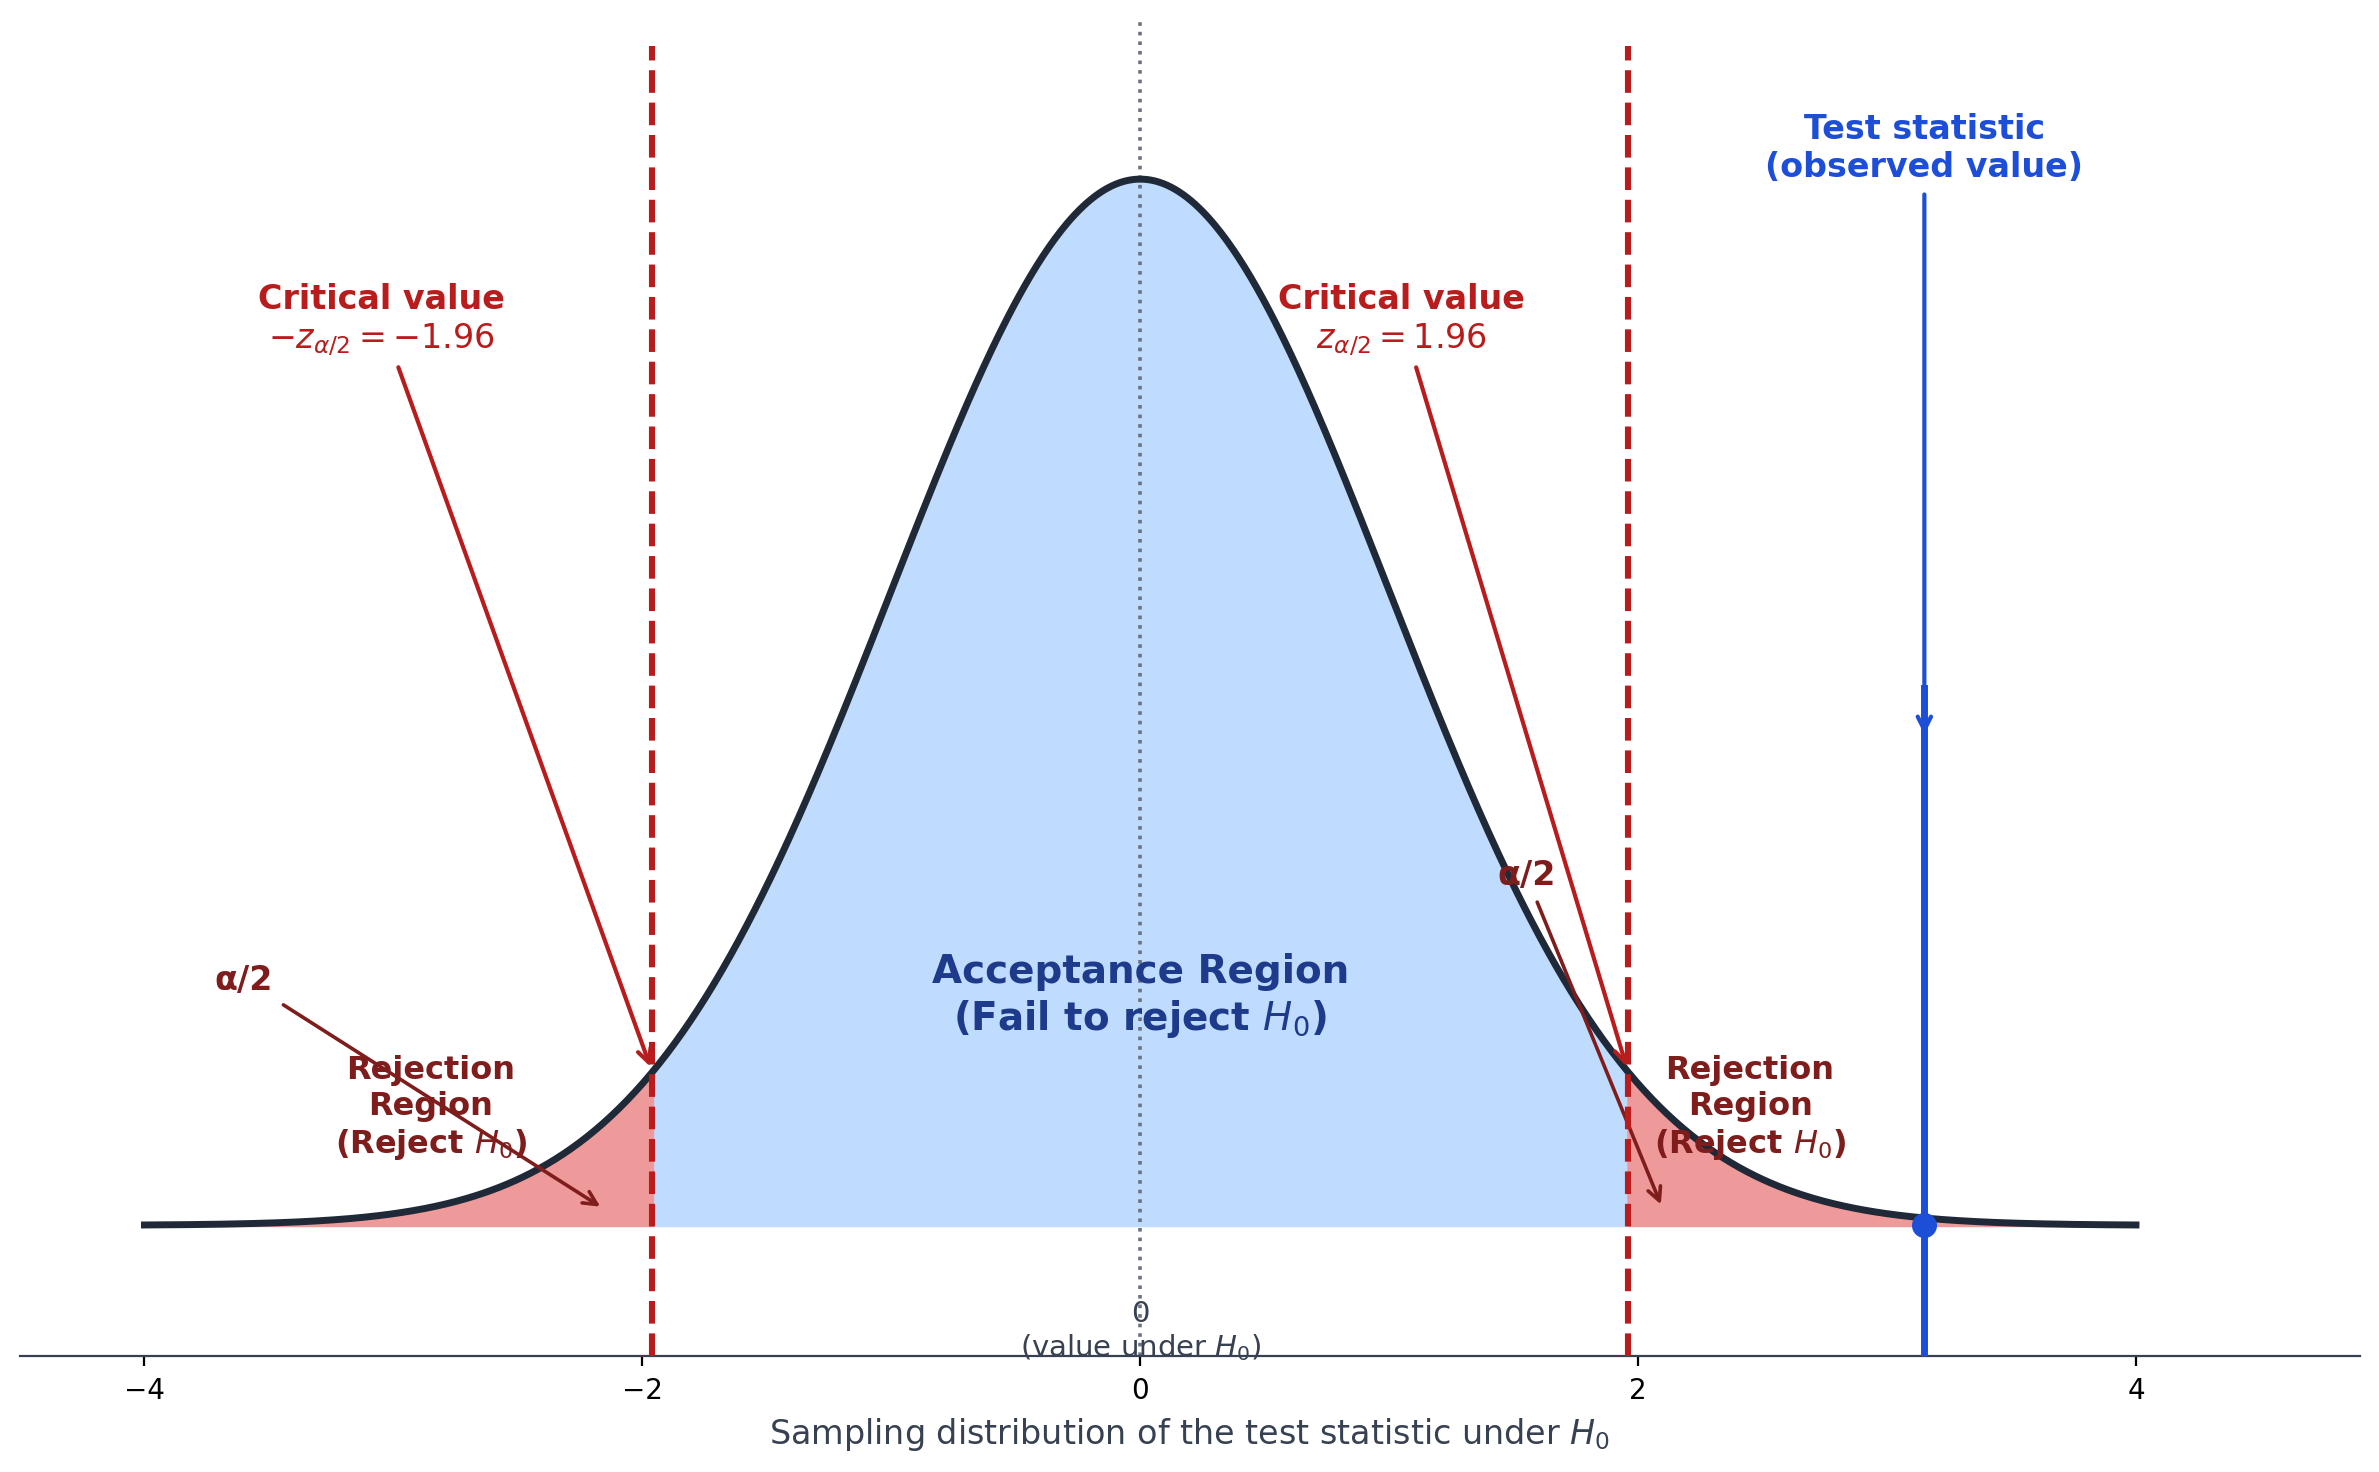
\includegraphics[width=5.85417in,height=\textheight,keepaspectratio]{Section2/images/two_tailed_critical_value.png}

\subsection{Worked Example}\label{worked-example-3}

A researcher tests whether a new drug changes mean blood pressure from
the population mean of \(\mu_0=130\) mmHg. A sample of \(n=36\) patients
gives \(\bar{x}=126\) mmHg, \(s=12\) mmHg. Test at \(\alpha=0.05\)
(two-tailed).

\textbf{Step 1:} State hypotheses: \(H_0: \mu=130\)
vs.~\(H_a: \mu\ne130\).

\textbf{Step 2:} Level of significance (\(\alpha=0.05\))

\textbf{Step 3:} Compute the test statistic (using \(z\) since \(n\) is
reasonably large)

\[ SE = s/\sqrt{n} = 12/\sqrt{36}=12/6=2.0 \]
\[z = \frac{\bar{x}-\mu_0}{SE} = \frac{126-130}{2.0} = -2.0\]

\textbf{Step 4:} Determine P-value or critical value

\begin{itemize}
\tightlist
\item
  Find the p-value for a two-tailed test:
\end{itemize}

\(p = 2\times P(Z\le-2.0) = 2\times0.0228=0.0456\).

\begin{itemize}
\tightlist
\item
  Critical value of Z at α=0.05 is -1.96 (from Z table)
\end{itemize}

\textbf{Step 5:} Decision and conclusion: When p-value is compared with
\(\alpha=0.05\) or critical value is compared with test statistics.
Since \(0.0456<0.05\) or -2.0 is less than -1.96, \(H_0\) is rejected.
Thus,there is statistically significant evidence, at the 5\% level, that
mean blood pressure differs from 130 mmHg.

\section{Statistical Significance vs.~Practical (Clinical)
Significance}\label{statistical-significance-vs.-practical-clinical-significance}

\textbf{Statistical significance} means the observed effect is unlikely
to have arisen from chance alone (p ≤ α), given the sample size and
variability. \textbf{Practical (or clinical) significance} asks whether
the size of the effect is large enough to matter in real-world,
clinical, or public health terms.

\begin{tcolorbox}[enhanced jigsaw, bottomrule=.15mm, breakable, opacityback=0, toptitle=1mm, titlerule=0mm, bottomtitle=1mm, colback=white, arc=.35mm, rightrule=.15mm, toprule=.15mm, leftrule=.75mm, title=\textcolor{quarto-callout-important-color}{\faExclamation}\hspace{0.5em}{Important}, colbacktitle=quarto-callout-important-color!10!white, colframe=quarto-callout-important-color-frame, coltitle=black, left=2mm, opacitybacktitle=0.6]

With a very large sample size, even a \textbf{tiny, clinically
meaningless difference} (e.g., a 0.5 mmHg drop in blood pressure) can be
statistically significant. Conversely, with a small sample, a
\textbf{large, clinically important effect} may fail to reach
statistical significance. Always report and interpret \textbf{effect
sizes and confidence intervals} alongside p-values, not p-values alone.

\end{tcolorbox}

\section{One-Tailed vs.~Two-Tailed
Tests}\label{one-tailed-vs.-two-tailed-tests}

\begin{itemize}
\item
  \textbf{Two-tailed test:} Tests for a difference in \textbf{either
  direction} (\(H_a: \mu \ne \mu_0\)). The rejection region is split
  between both tails of the distribution.
\item
  \textbf{One-tailed test:} Tests for a difference in \textbf{one
  specific direction} only (\(H_a: \mu>\mu_0\) or \(H_a:\mu<\mu_0\)).
  The entire rejection region is in one tail. It can be right tailed and
  left tailed

  \begin{longtable}[]{@{}
    >{\raggedright\arraybackslash}p{(\linewidth - 2\tabcolsep) * \real{0.5060}}
    >{\raggedright\arraybackslash}p{(\linewidth - 2\tabcolsep) * \real{0.4940}}@{}}
  \toprule\noalign{}
  \endhead
  \bottomrule\noalign{}
  \endlastfoot
  \begin{minipage}[t]{\linewidth}\raggedright
  \begin{figure}[H]

  {\centering 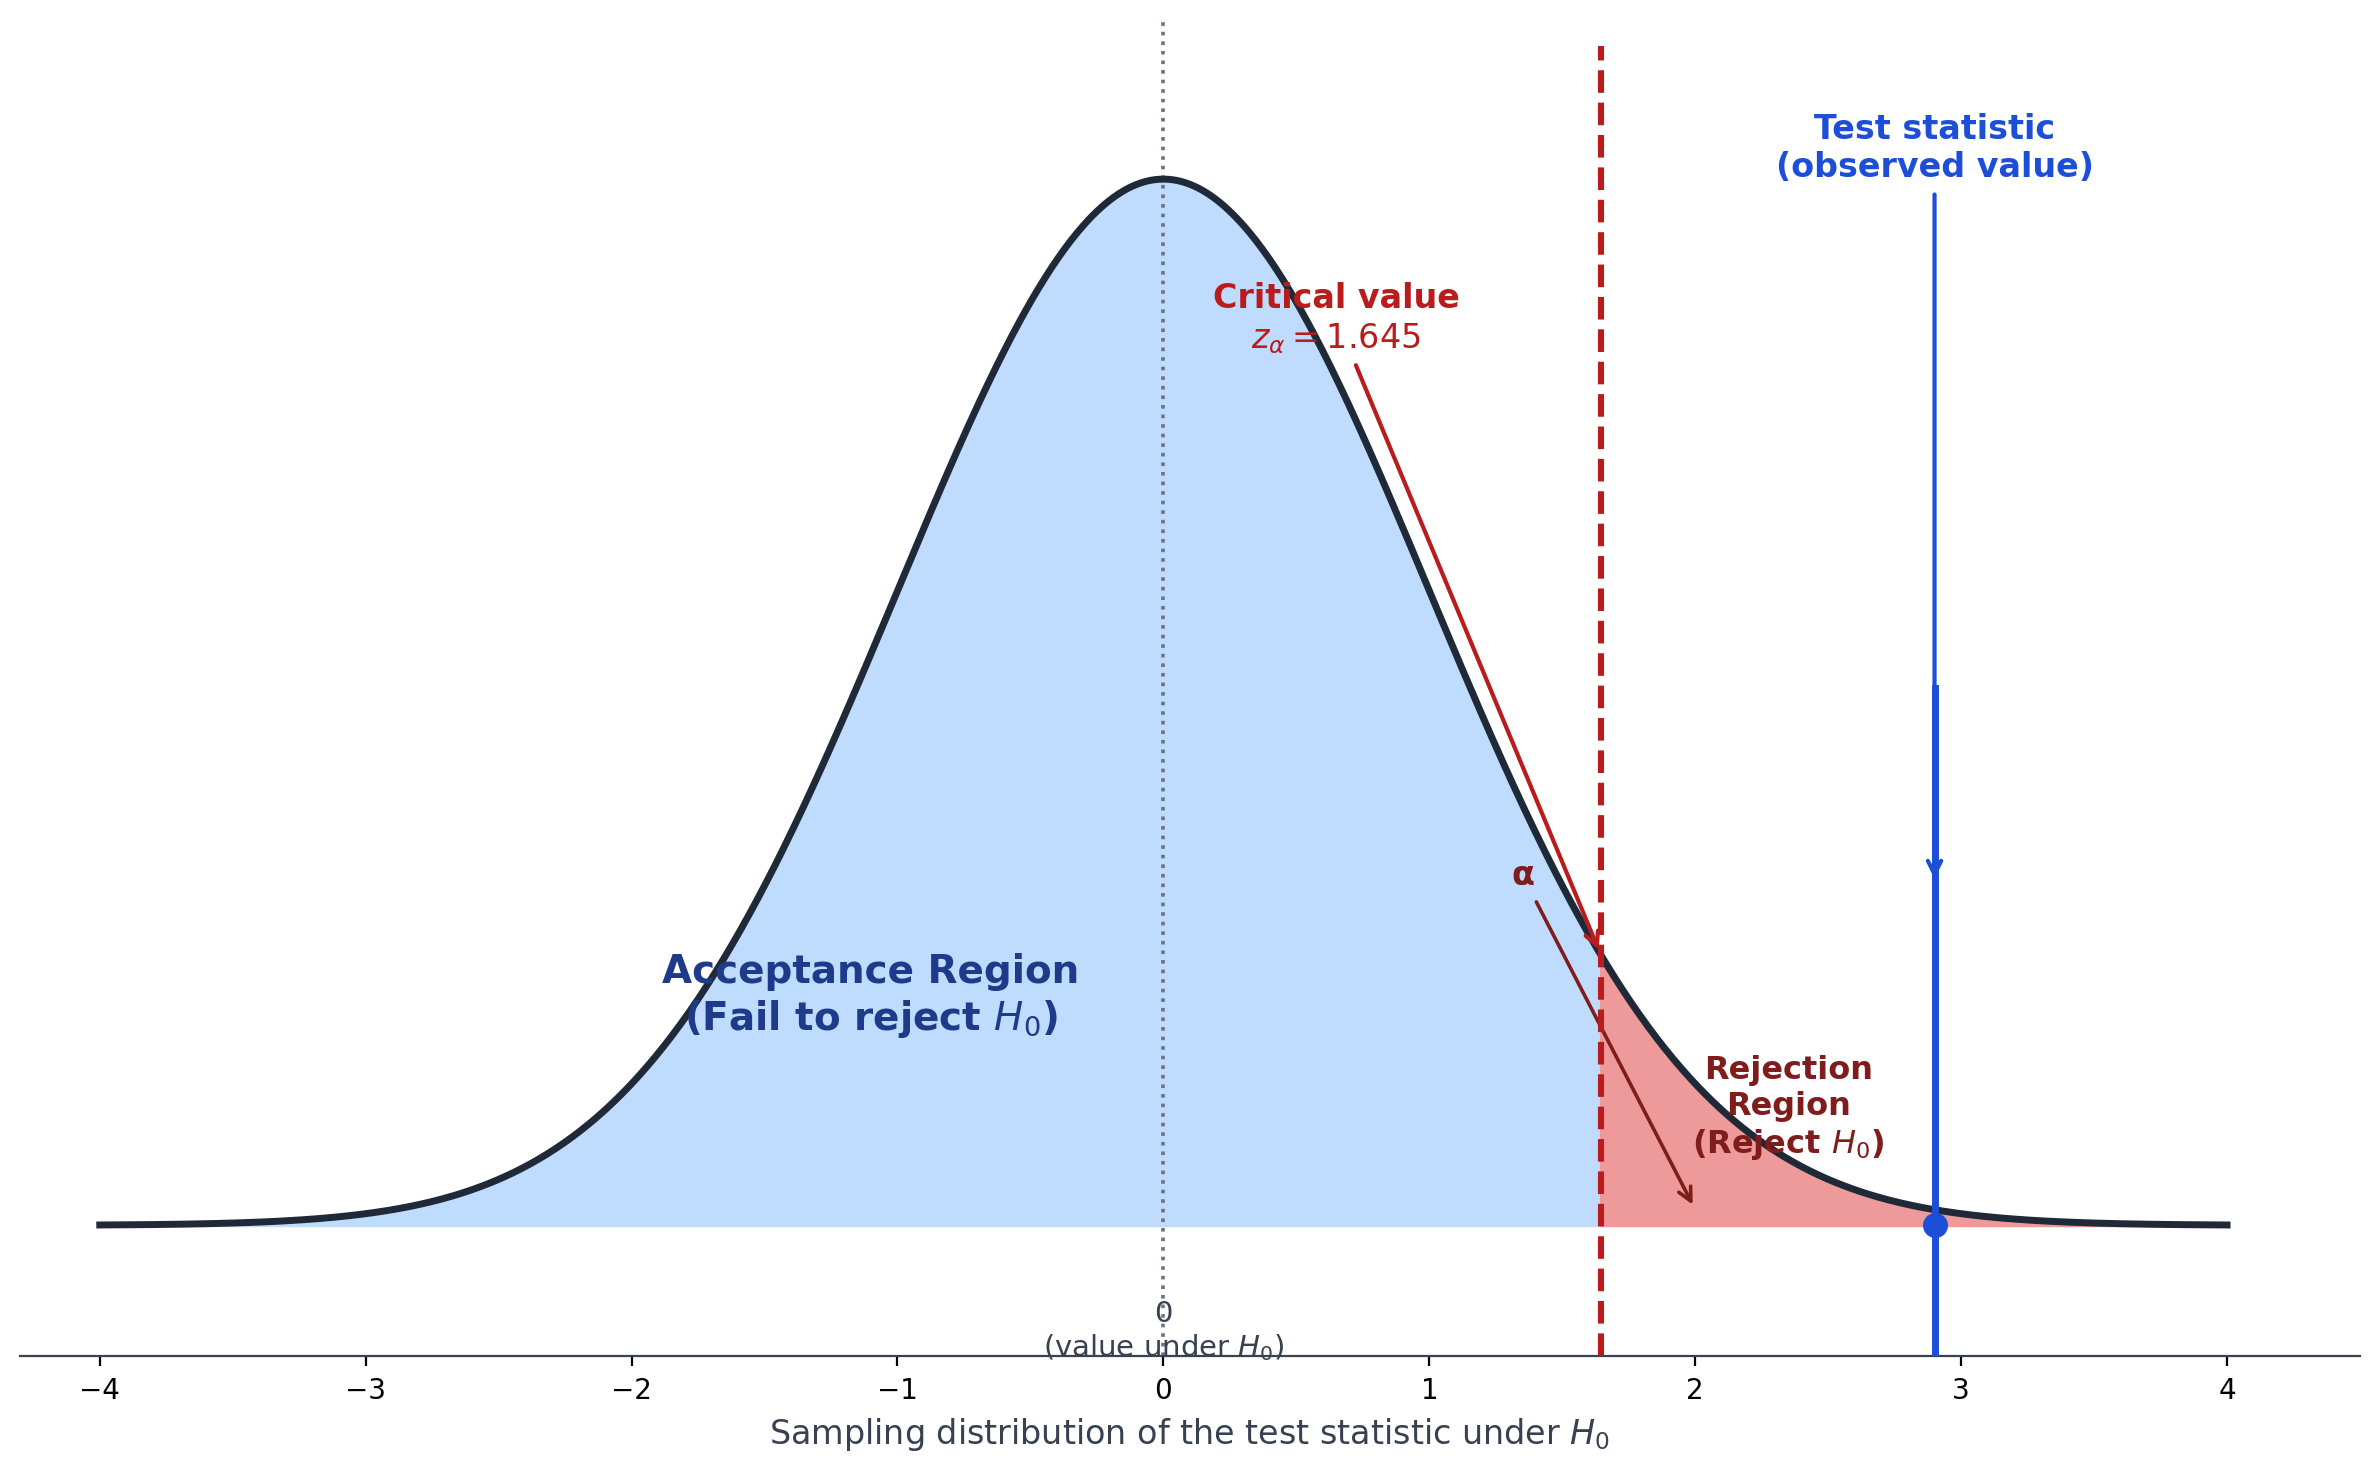
\includegraphics[width=5.42708in,height=\textheight,keepaspectratio]{Section2/images/right_tailed_test.png}

  }

  \caption{Figure: Right-tailed hypothesis test}

  \end{figure}%
  \end{minipage} & \begin{minipage}[t]{\linewidth}\raggedright
  \begin{figure}[H]

  {\centering 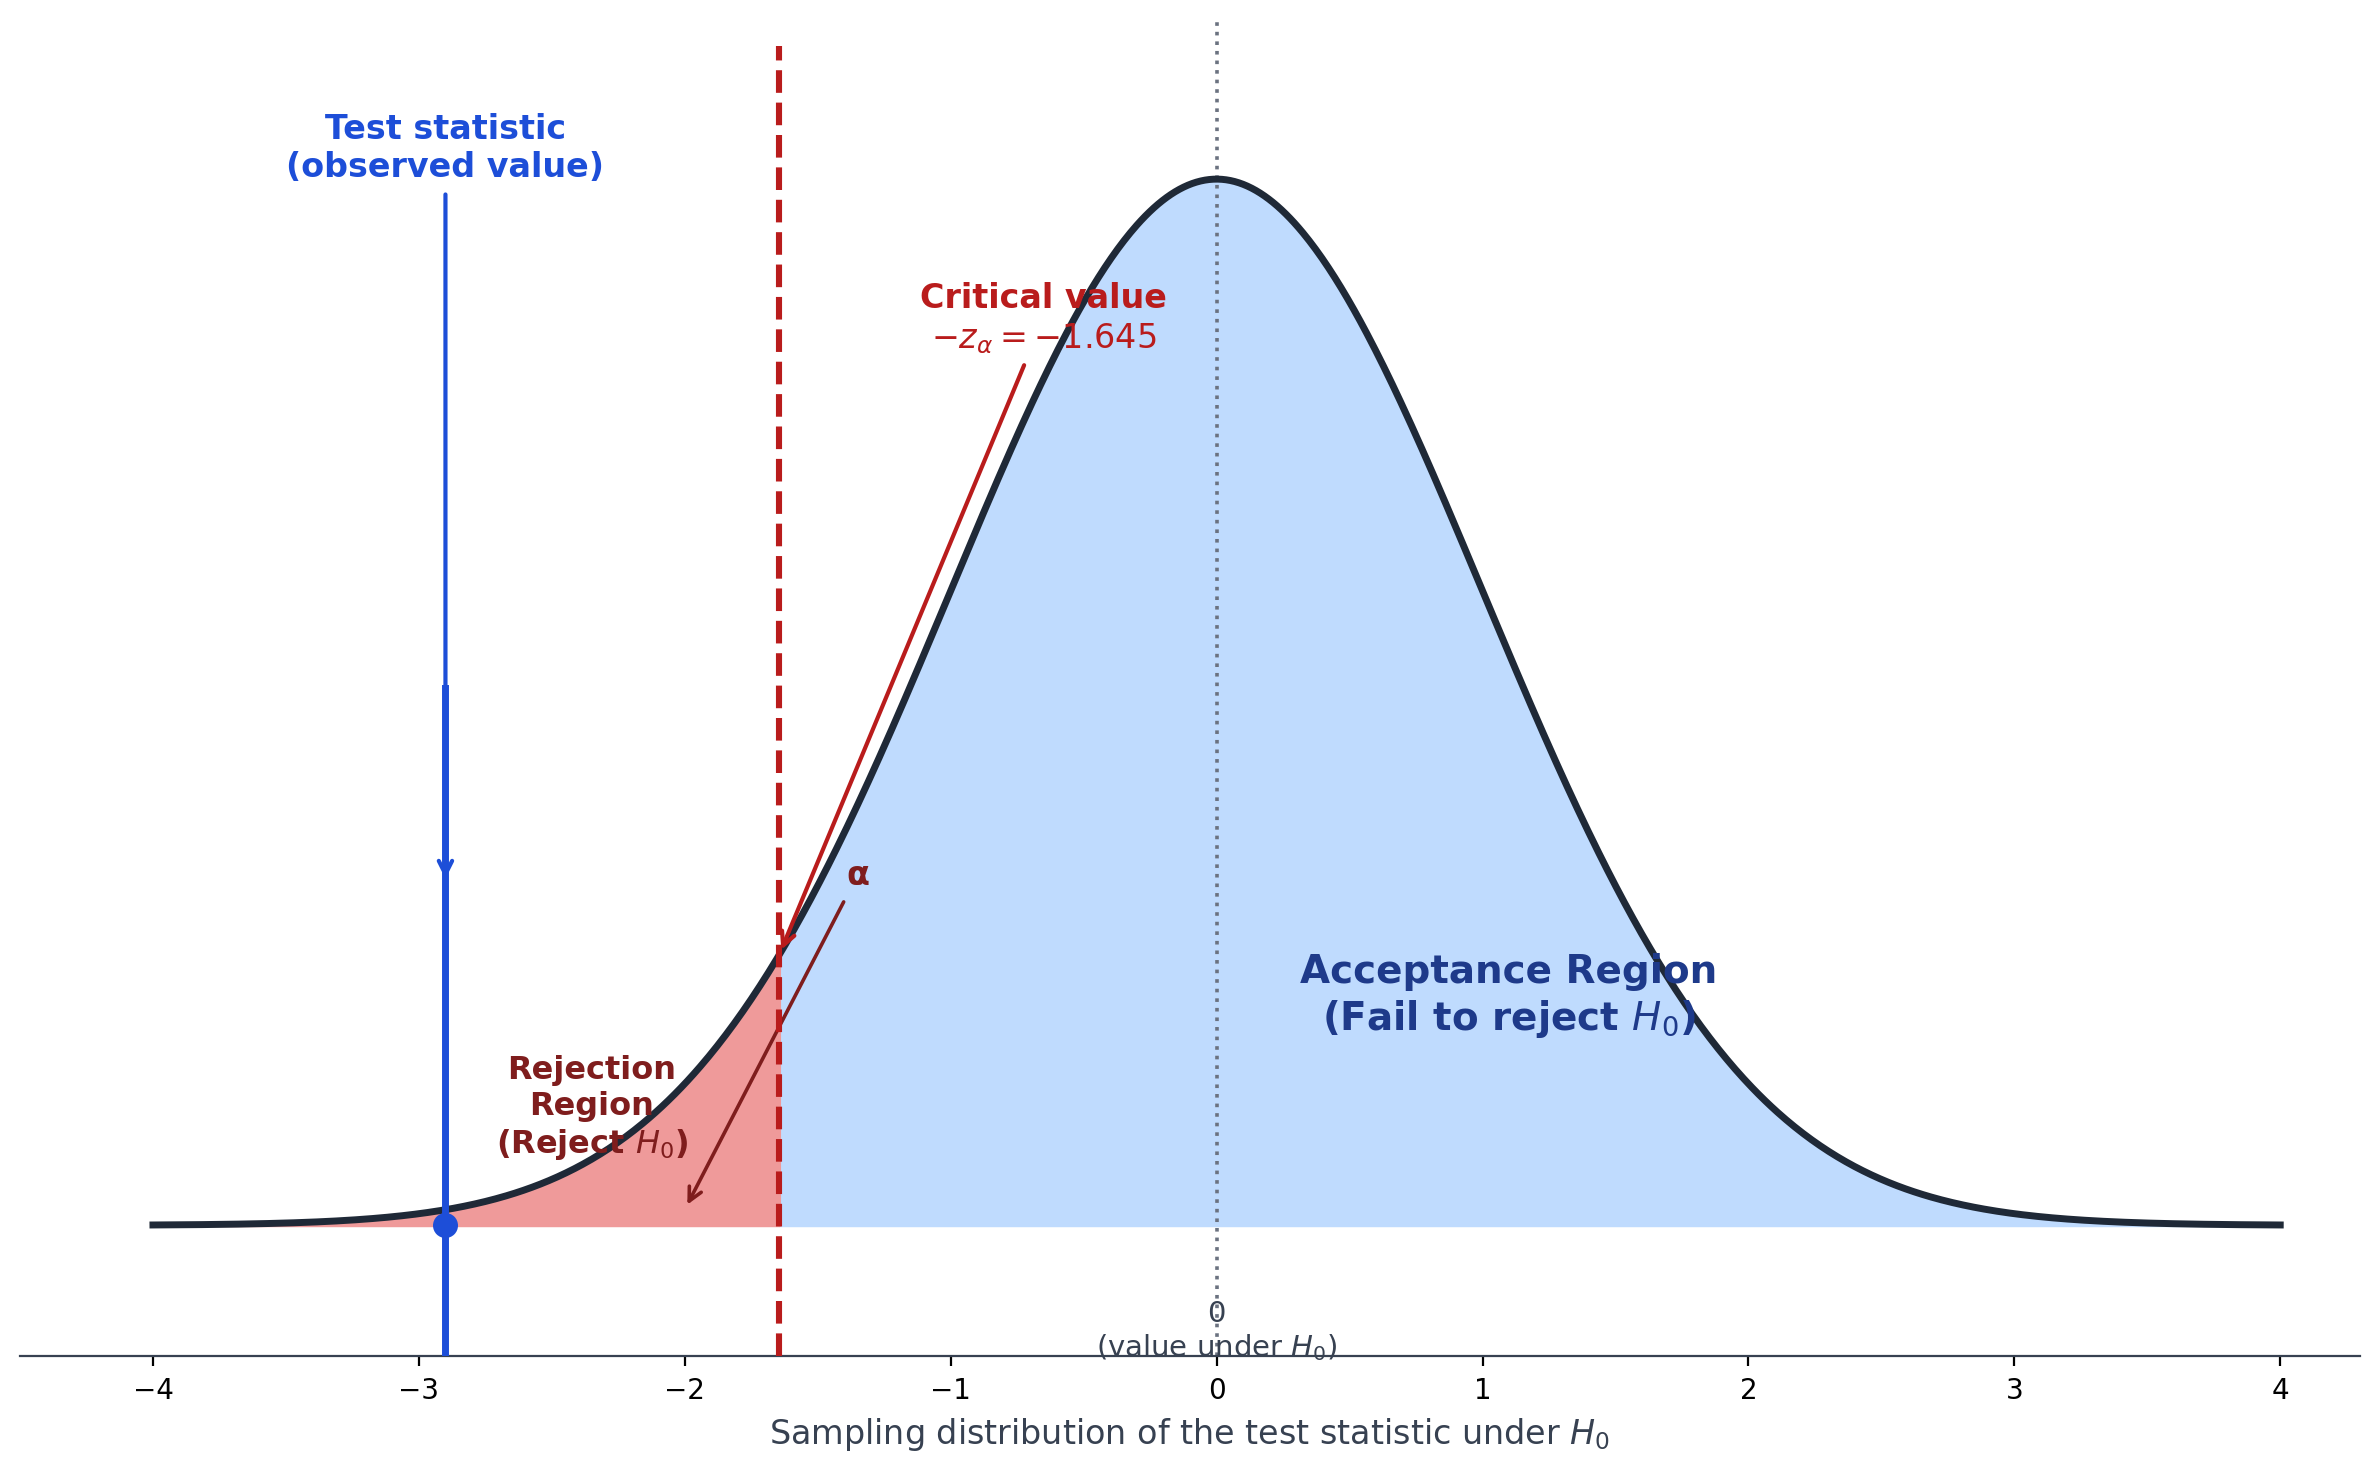
\includegraphics[width=5.39583in,height=\textheight,keepaspectratio]{Section2/images/left_tailed_test.png}

  }

  \caption{Figure: Left-tailed hypothesis test}

  \end{figure}%
  \end{minipage} \\
  \end{longtable}
\end{itemize}

\textbf{Choosing a tail:} A one-tailed test should be specified
\textbf{before} looking at the data and only when there is a strong a
priori reason to test in only one direction (e.g., testing whether a new
drug is \emph{better than} placebo, not just \emph{different}).
Two-tailed tests are more conservative and are the standard default in
most biomedical research.

\chapter{Types of Errors}\label{types-of-errors}

Every hypothesis test decision (reject \(H_0\) or fail to reject
\(H_0\)) can be right or wrong, because the decision is based on a
\textbf{sample}, not the entire population. There are two distinct ways
to be wrong: \textbf{Type I error} and \textbf{Type II error}.

\section{The Decision Matrix}\label{the-decision-matrix}

\begin{longtable}[]{@{}
  >{\raggedright\arraybackslash}p{(\linewidth - 4\tabcolsep) * \real{0.2368}}
  >{\raggedright\arraybackslash}p{(\linewidth - 4\tabcolsep) * \real{0.4035}}
  >{\raggedright\arraybackslash}p{(\linewidth - 4\tabcolsep) * \real{0.3509}}@{}}
\toprule\noalign{}
\begin{minipage}[b]{\linewidth}\raggedright
\end{minipage} & \begin{minipage}[b]{\linewidth}\raggedright
\(H_0\) is actually True
\end{minipage} & \begin{minipage}[b]{\linewidth}\raggedright
\(H_0\) is actually False
\end{minipage} \\
\midrule\noalign{}
\endhead
\bottomrule\noalign{}
\endlastfoot
\textbf{Reject} \(H_0\) & Type I Error (probability = \(\alpha\)) &
Correct decision (power = \(1-\beta\)) \\
\textbf{Fail to reject} \(H_0\) & Correct decision (probability =
\(1-\alpha\)) & Type II Error (probability = \(\beta\)) \\
\end{longtable}

\section{Type I Error}\label{type-i-error}

\begin{tcolorbox}[enhanced jigsaw, bottomrule=.15mm, breakable, opacityback=0, toptitle=1mm, titlerule=0mm, bottomtitle=1mm, colback=white, arc=.35mm, rightrule=.15mm, toprule=.15mm, leftrule=.75mm, title=\textcolor{quarto-callout-note-color}{\faInfo}\hspace{0.5em}{Note}, colbacktitle=quarto-callout-note-color!10!white, colframe=quarto-callout-note-color-frame, coltitle=black, left=2mm, opacitybacktitle=0.6]

\textbf{Type I error} occurs when we \textbf{reject a true null
hypothesis}, concluding that there is an effect/difference when, in
reality, there is none. This is a \textbf{``false positive''} finding.
Its probability is exactly \(\alpha\), the significance level chosen by
the researcher.

\end{tcolorbox}

\textbf{Clinical example:} Concluding that a new drug lowers blood
pressure more effectively than the standard treatment, when in truth the
two treatments are equally effective leading to unnecessary adoption of
a more expensive or riskier drug with no real benefit.

\section{Type II Error}\label{type-ii-error}

\begin{tcolorbox}[enhanced jigsaw, bottomrule=.15mm, breakable, opacityback=0, toptitle=1mm, titlerule=0mm, bottomtitle=1mm, colback=white, arc=.35mm, rightrule=.15mm, toprule=.15mm, leftrule=.75mm, title=\textcolor{quarto-callout-note-color}{\faInfo}\hspace{0.5em}{Note}, colbacktitle=quarto-callout-note-color!10!white, colframe=quarto-callout-note-color-frame, coltitle=black, left=2mm, opacitybacktitle=0.6]

\textbf{Type II error} occurs when we \textbf{fail to reject a false
null hypothesis} concluding that there is no effect/difference when, in
reality, one exists. This is a \textbf{``false negative''} finding. Its
probability is denoted \(\beta\).

\end{tcolorbox}

\textbf{Clinical example:} Concluding that a new drug is no more
effective than the standard treatment, when it actually is effective
leading to a genuinely beneficial treatment being abandoned or never
adopted.

\section{Statistical Power}\label{statistical-power}

\textbf{Power} is the probability of \textbf{correctly rejecting a false
null hypothesis}. It is correctly detecting a real effect when one truly
exists: \[\text{Power} = 1-\beta\]

Power is influenced by four main factors:

\begin{enumerate}
\def\labelenumi{\arabic{enumi}.}
\tightlist
\item
  \textbf{Sample size (}\(n\)): Larger samples increase power (more
  precise estimates, smaller standard errors).
\item
  \textbf{Effect size:} Larger true differences between groups are
  easier to detect, increasing power.
\item
  \textbf{Significance level (}\(\alpha\)): A larger \(\alpha\) (e.g.,
  0.10 instead of 0.05) increases power but also increases the Type I
  error rate. There is a direct trade-off between power and Type-I
  error.
\item
  \textbf{Variability in the data (}\(\sigma\)): Less variability
  (noise) increases power.
\end{enumerate}

Conventionally, studies are designed to achieve \textbf{power}
\(\ge 80\%\) (i.e., \(\beta \le 0.20\)), meaning there is at least an
80\% chance of detecting a true effect of the specified size if it
exists. These parameters are used to calculate sample size during study
design and \emph{before} data collection.

\section{Confidence Level}\label{confidence-level}

The \textbf{confidence level} (\(1-\alpha\)) is the complement of the
Type I error rate, and represents the long-run proportion of confidence
intervals (constructed the same way, from repeated samples) that would
contain the true population parameter. A 95\% confidence level
corresponds to \(\alpha=0.05\). Confidence intervals are covered in
depth later in this chapter.

\section{\texorpdfstring{Relationship Among \(\alpha\), \(\beta\), and
Power}{Relationship Among \textbackslash alpha, \textbackslash beta, and Power}}\label{relationship-among-alpha-beta-and-power}

\begin{figure}[H]

{\centering \pandocbounded{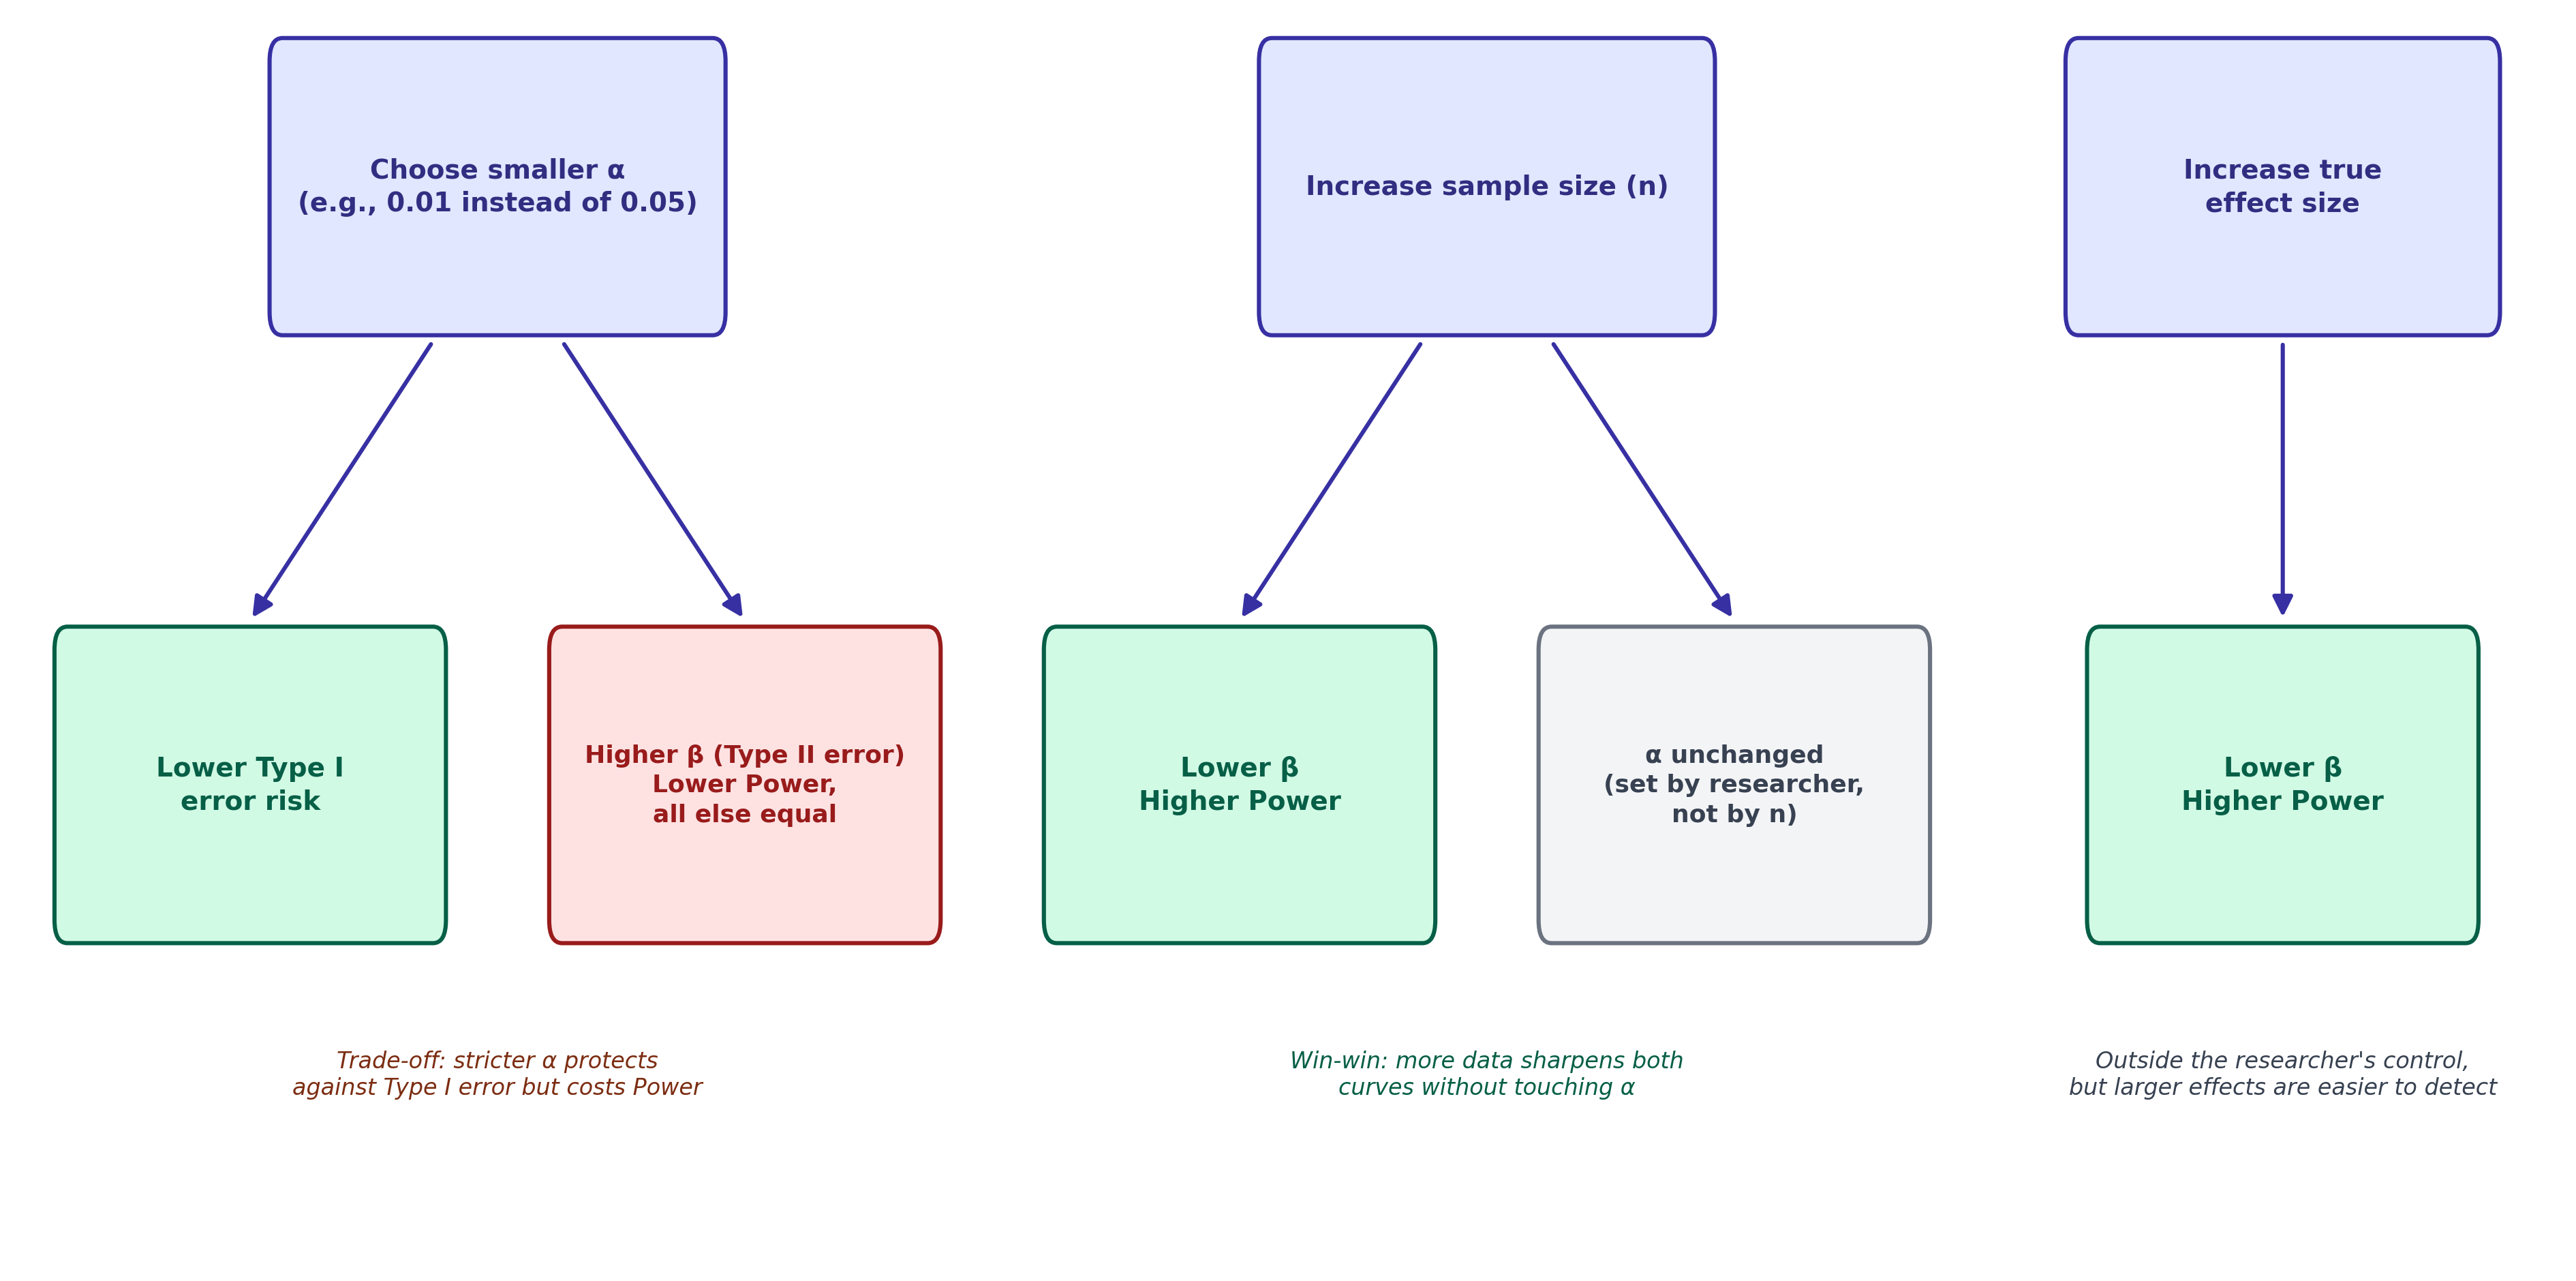
\includegraphics[keepaspectratio]{Section2/images/alpha_beta_power_relationships.png}}

}

\caption{Relationship between alpha error , beta error and power}

\end{figure}%

\begin{tcolorbox}[enhanced jigsaw, bottomrule=.15mm, breakable, opacityback=0, toptitle=1mm, titlerule=0mm, bottomtitle=1mm, colback=white, arc=.35mm, rightrule=.15mm, toprule=.15mm, leftrule=.75mm, title=\textcolor{quarto-callout-important-color}{\faExclamation}\hspace{0.5em}{Important}, colbacktitle=quarto-callout-important-color!10!white, colframe=quarto-callout-important-color-frame, coltitle=black, left=2mm, opacitybacktitle=0.6]

There is an inherent \textbf{trade-off between} \(\alpha\) and \(\beta\)
for a \emph{fixed} sample size: reducing the Type I error rate (using a
smaller \(\alpha\), e.g., 0.01 instead of 0.05) makes it harder to
reject \(H_0\), which \textbf{increases} the Type II error rate
(\(\beta\)) and \textbf{decreases} power --- unless sample size is also
increased to compensate. Increasing sample size is the primary way to
reduce \(\beta\) (increase power) \textbf{without} increasing
\(\alpha\).

\end{tcolorbox}

\section{Worked Example (Illustrating the
Trade-off)}\label{worked-example-illustrating-the-trade-off}

A clinical trial is designed to detect a 5 mmHg reduction in blood
pressure. With \(n=30\) per group, the study has 60\% power at
\(\alpha=0.05\) --- meaning there is a 40\% chance (\(\beta=0.40\)) of
\textbf{missing} a true 5 mmHg effect (a Type II error) if it exists. To
increase power to the conventional 80\% threshold while keeping
\(\alpha=0.05\) fixed, the researcher must \textbf{increase the sample
size} (e.g., to \(n=64\) per group, calculated using standard
power-analysis formulas) --- sample size calculation is covered in a
dedicated chapter later in this book.

\section{\texorpdfstring{Diagram: Overlapping Sampling Distributions
Under \(H_0\) and
\(H_a\)}{Diagram: Overlapping Sampling Distributions Under H\_0 and H\_a}}\label{diagram-overlapping-sampling-distributions-under-h_0-and-h_a}

\pandocbounded{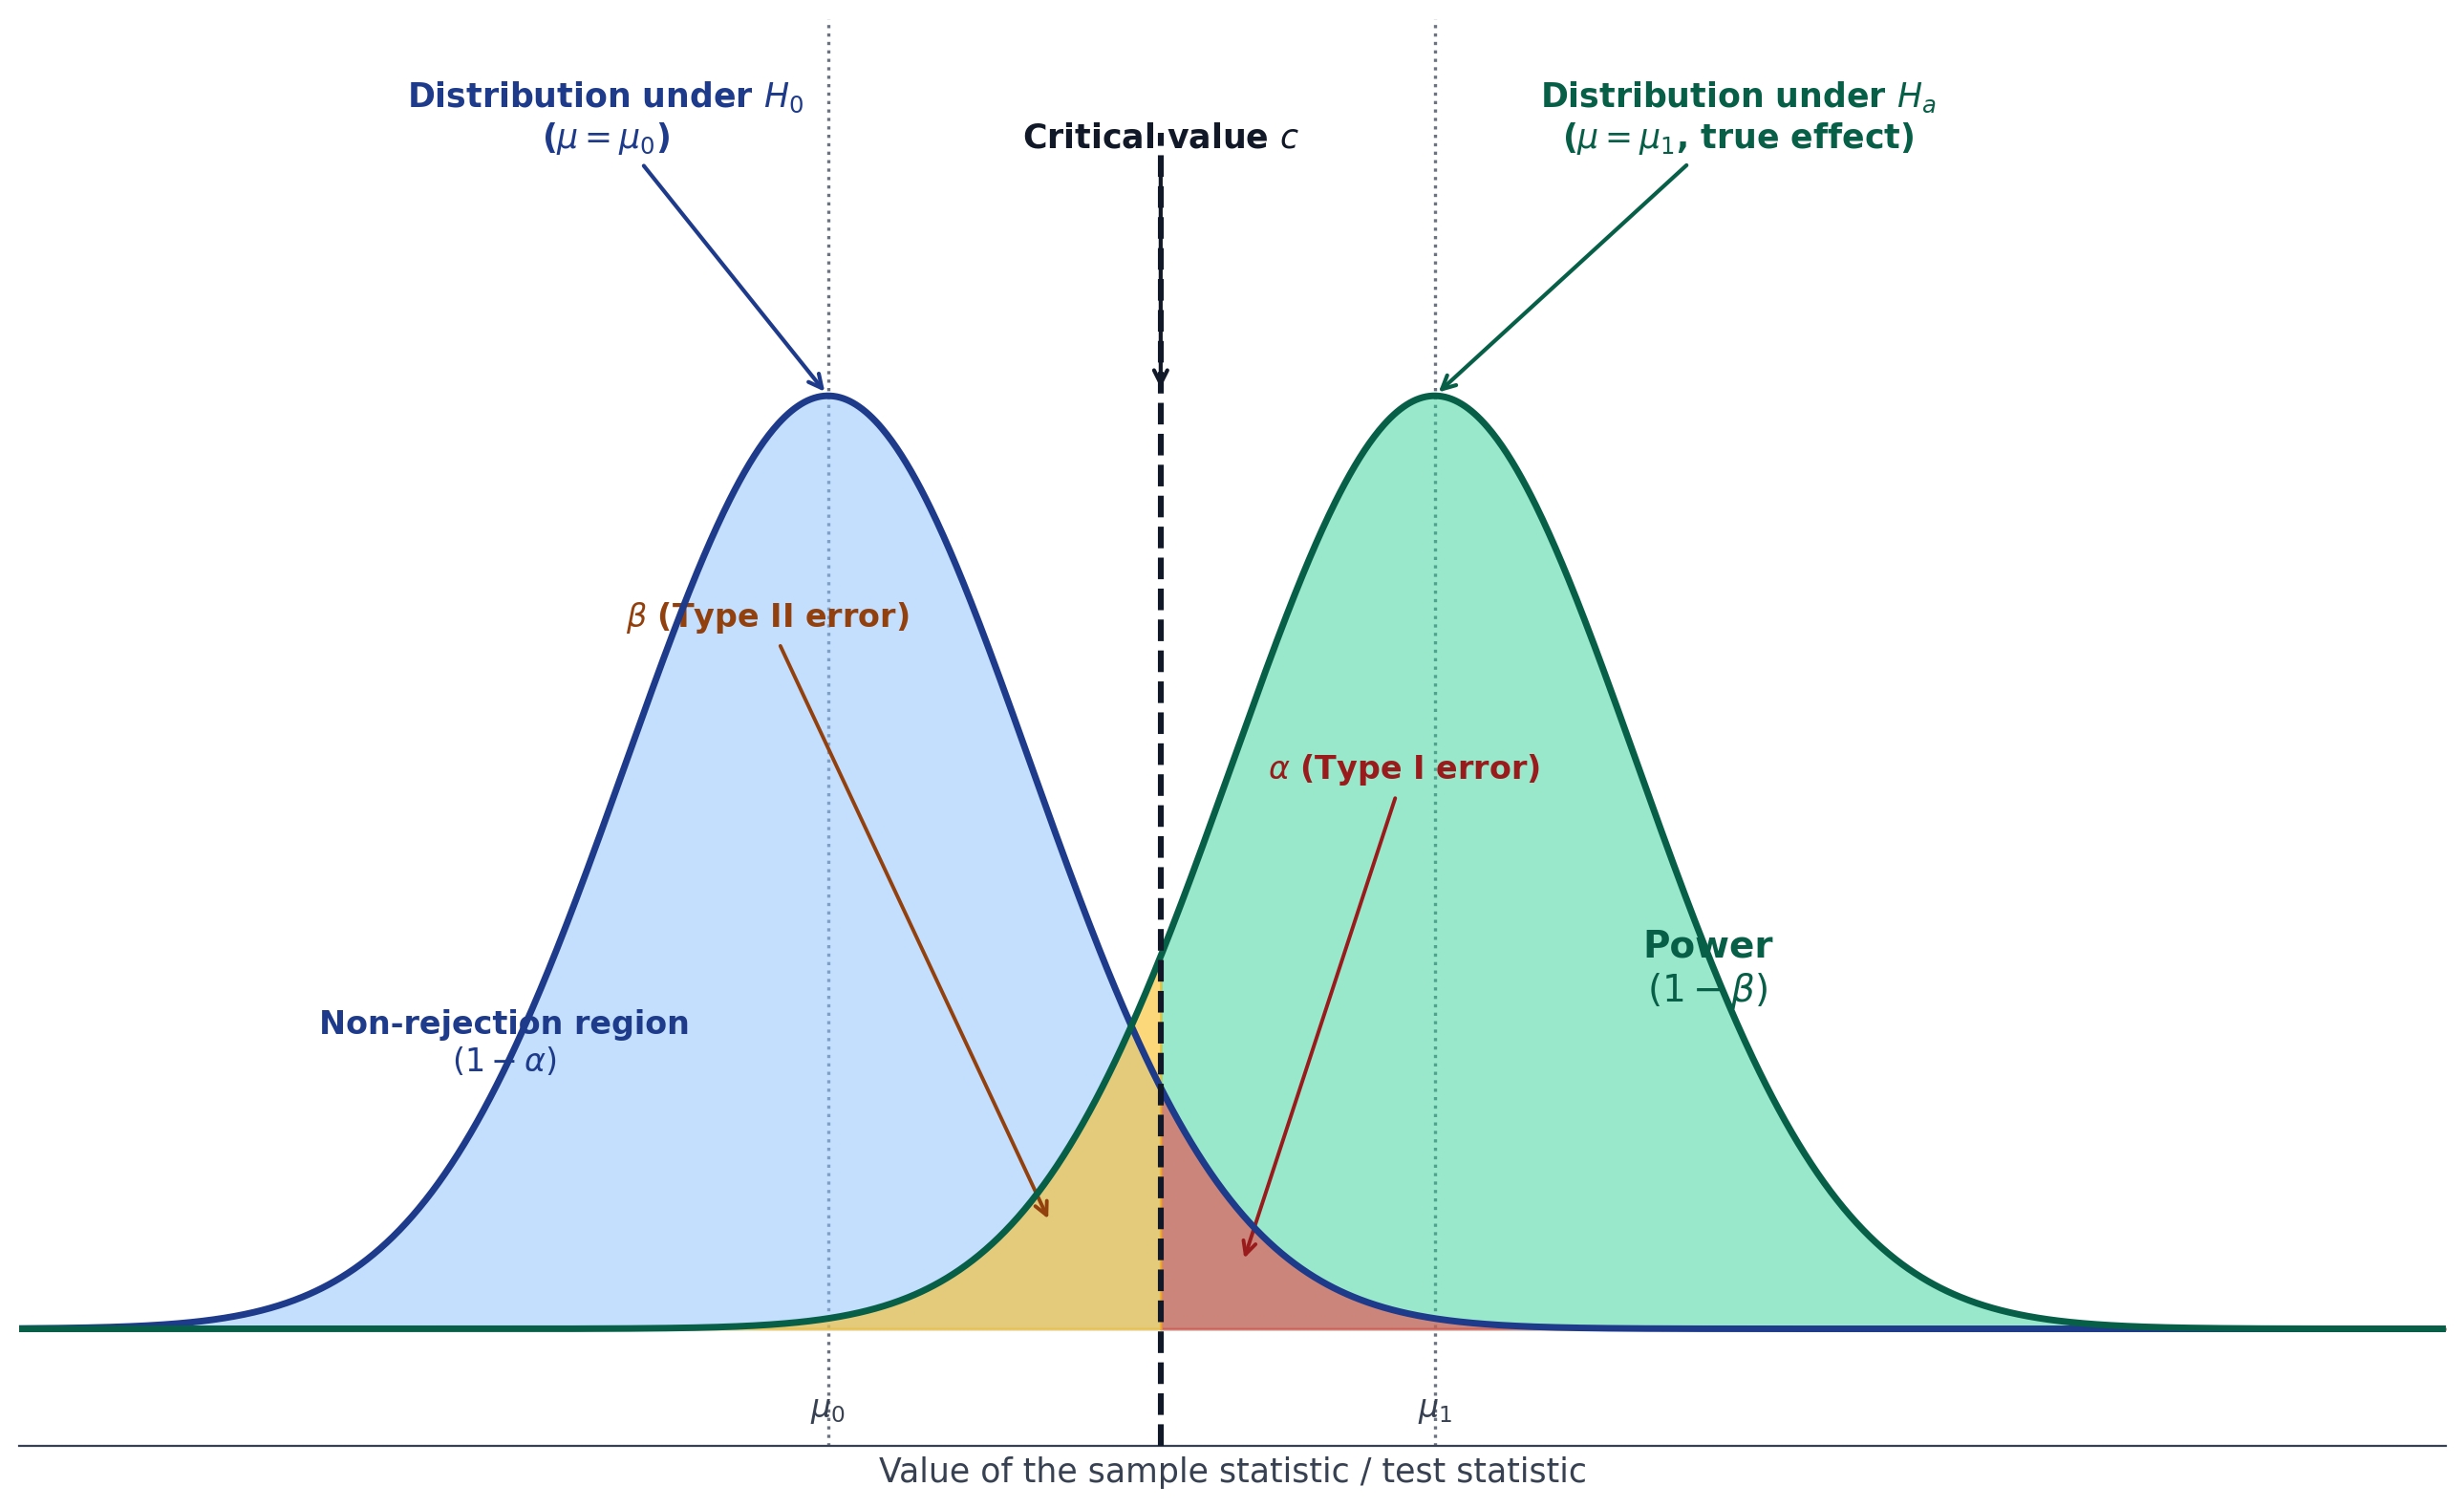
\includegraphics[keepaspectratio]{Section2/images/h0_ha_alpha_beta_power.png}}

The critical value that defines \(\alpha\) under \(H_0\) simultaneously
defines \(\beta\) under \(H_a\) --- the two error rates are linked
through the same decision threshold, which is why changing \(\alpha\)
mechanically changes \(\beta\) (for fixed \(n\) and effect size).

\chapter{Estimation}\label{estimation}

\textbf{Estimation} is the process of using sample data to infer the
value of an unknown population parameter. There are two complementary
approaches: \textbf{point estimation} (a single best-guess value) and
\textbf{interval estimation} (a range of plausible values that also
conveys the precision of the estimate).

\section{Point Estimation}\label{point-estimation}

A \textbf{point estimate} is a single numeric value, calculated from
sample data, that serves as the ``best guess'' for a population
parameter.

\begin{longtable}[]{@{}
  >{\raggedright\arraybackslash}p{(\linewidth - 2\tabcolsep) * \real{0.5132}}
  >{\raggedright\arraybackslash}p{(\linewidth - 2\tabcolsep) * \real{0.4868}}@{}}
\toprule\noalign{}
\begin{minipage}[b]{\linewidth}\raggedright
Population Parameter
\end{minipage} & \begin{minipage}[b]{\linewidth}\raggedright
Point Estimator (Sample Statistic)
\end{minipage} \\
\midrule\noalign{}
\endhead
\bottomrule\noalign{}
\endlastfoot
\(\mu\) (population mean) & \(\bar{x}\) (sample mean) \\
\(\sigma^2\) (population variance) & \(s^2\) (sample variance) \\
\(\pi\) or \(P\) (population proportion) & \(\hat{p}\) (sample
proportion) \\
\end{longtable}

\textbf{Desirable properties of a good point estimator:} unbiasedness
(its expected value equals the true parameter, e.g.,
\(E(\bar{x})=\mu\)), consistency (it converges to the true parameter as
\(n\to\infty\)), and efficiency (it has the smallest possible variance
among unbiased estimators).

\begin{tcolorbox}[enhanced jigsaw, bottomrule=.15mm, breakable, opacityback=0, toptitle=1mm, titlerule=0mm, bottomtitle=1mm, colback=white, arc=.35mm, rightrule=.15mm, toprule=.15mm, leftrule=.75mm, title=\textcolor{quarto-callout-important-color}{\faExclamation}\hspace{0.5em}{Important}, colbacktitle=quarto-callout-important-color!10!white, colframe=quarto-callout-important-color-frame, coltitle=black, left=2mm, opacitybacktitle=0.6]

A point estimate alone gives \textbf{no information about its precision
or reliability}. A sample mean of \(\bar{x}=126\) mmHg conveys nothing
about how much uncertainty surrounds that estimate. Was it based on 10
patients or 10,000? \textbf{Interval estimation} solves this problem.

\end{tcolorbox}

\section{Standard Error}\label{standard-error}

The \textbf{standard error (SE)} is the standard deviation of the
sampling distribution of a statistic --- it quantifies how much a sample
statistic (like \(\bar{x}\)) would vary from sample to sample if we
repeated the sampling process many times.

\[SE(\bar{x}) = \frac{s}{\sqrt{n}} \qquad SE(\hat{p}) = \sqrt{\frac{\hat{p}(1-\hat{p})}{n}}\]

\begin{tcolorbox}[enhanced jigsaw, bottomrule=.15mm, breakable, opacityback=0, toptitle=1mm, titlerule=0mm, bottomtitle=1mm, colback=white, arc=.35mm, rightrule=.15mm, toprule=.15mm, leftrule=.75mm, title=\textcolor{quarto-callout-tip-color}{\faLightbulb}\hspace{0.5em}{Tip}, colbacktitle=quarto-callout-tip-color!10!white, colframe=quarto-callout-tip-color-frame, coltitle=black, left=2mm, opacitybacktitle=0.6]

Do not confuse \textbf{standard deviation (SD)} with \textbf{standard
error (SE)}. The SD describes variability of \textbf{individual
observations} in the data; the SE describes variability of the
\textbf{sample statistic itself} (e.g., the mean) across repeated
samples. As \(n\) increases, SD stays roughly constant (it reflects the
population), but SE \textbf{shrinks} (larger samples give more
precise/stable estimates of the mean), because \(SE = s/\sqrt{n}\).

\end{tcolorbox}

\section{Interval Estimation and the Confidence
Interval}\label{interval-estimation-and-the-confidence-interval}

\subsection{Definition}\label{definition-25}

A \textbf{confidence interval (CI)} is a range of values, calculated
from sample data, that is likely to contain the true population
parameter, along with a stated \textbf{confidence level} (e.g., 95\%)
reflecting the long-run reliability of the method used to construct it.

\subsection{General Formula}\label{general-formula}

\[\text{Point estimate} \pm (\text{Critical value}) \times (\text{Standard error})\]
where,

\(Margin.of.error(ME)=critical.value \times standard.error\)

\subsection{Confidence Interval for a
Mean}\label{confidence-interval-for-a-mean}

When \(\sigma\) is unknown, we use \(t\) statistics,

\[\bar{x} \pm t_{\alpha/2, n-1} \times \frac{s}{\sqrt{n}}\]

\subsection{Confidence Interval for a
Proportion}\label{confidence-interval-for-a-proportion}

\[\hat{p} \pm z_{\alpha/2}\times\sqrt{\frac{\hat{p}(1-\hat{p})}{n}}\]

\section{Margin of Error}\label{margin-of-error}

The \textbf{margin of error (ME)} is the ``plus-or-minus'' part of the
confidence interval:
\[ME = (\text{Critical value})\times(\text{Standard error})\]

A larger margin of error means a wider, less precise interval; margin of
error decreases as sample size increases (since \(SE\) shrinks) and
increases as the desired confidence level increases (a higher critical
value is needed for more confidence).

\section{Confidence Level and Its
Interpretation}\label{confidence-level-and-its-interpretation}

Common confidence levels and their corresponding critical \(z\)-values
(for large samples/known \(\sigma\)):

\begin{longtable}[]{@{}lll@{}}
\toprule\noalign{}
Confidence Level & \(\alpha\) & Critical \(z_{\alpha/2}\) \\
\midrule\noalign{}
\endhead
\bottomrule\noalign{}
\endlastfoot
90\% & 0.10 & 1.645 \\
95\% & 0.05 & 1.96 \\
99\% & 0.01 & 2.576 \\
\end{longtable}

\begin{tcolorbox}[enhanced jigsaw, bottomrule=.15mm, breakable, opacityback=0, toptitle=1mm, titlerule=0mm, bottomtitle=1mm, colback=white, arc=.35mm, rightrule=.15mm, toprule=.15mm, leftrule=.75mm, title=\textcolor{quarto-callout-important-color}{\faExclamation}\hspace{0.5em}{Important}, colbacktitle=quarto-callout-important-color!10!white, colframe=quarto-callout-important-color-frame, coltitle=black, left=2mm, opacitybacktitle=0.6]

\textbf{Correct interpretation of a 95\% CI:} ``If we were to repeat
this study many times, drawing a new random sample each time and
constructing a CI the same way, approximately 95\% of those intervals
would contain the true population parameter.'' \textbf{It is incorrect}
to say ``there is a 95\% probability that the true parameter lies in
this particular interval''. Under the frequentist framework, the true
parameter is a fixed (though unknown) constant, and any single computed
interval either contains it or does not (this is closer to the Bayesian
\emph{credible interval} interpretation).

\end{tcolorbox}

\section{Worked Example (Confidence interval for a
mean)}\label{worked-example-confidence-interval-for-a-mean}

Using our earlier sample: \(n=36\) patients, \(\bar{x}=126\) mmHg,
\(s=12\) mmHg. Construct a 95\% CI for the true mean blood pressure.

\textbf{Step 1:} Compute the standard error:
\(SE = s/\sqrt{n} = 12/\sqrt{36} = 2.0\).

\textbf{Step 2:} Find the critical value: for a 95\% CI with \(n-1=35\)
df

\(t_{0.025,35}\approx 2.03\) (close to the \(z\) value of 1.96 for large
\(n\)).

\textbf{Step 3:} Compute the margin of error:
\(ME = 2.03\times2.0=4.06\).

\textbf{Step 4:} Construct the interval:
\[126 \pm 4.06 = (121.9,\ 130.1) \text{ mmHg}\]

\textbf{Interpretation:} We are 95\% confident that the true mean blood
pressure of the population from which this sample was drawn lies between
121.9 and 130.1 mmHg. Note this interval \textbf{includes} 130 mmHg, the
value tested in Section 9's hypothesis test --- consistent with that
test's borderline result (p = 0.046, just below 0.05, so technically
still significant, illustrating that CIs and hypothesis tests can appear
to be right at the boundary of agreement/disagreement when a result is
only marginally significant).

\section{Determine the confidence interval around mean in
R}\label{determine-the-confidence-interval-around-mean-in-r}

We can use \texttt{meanCI()} from \textbf{DescTools} to calculate CI
around mean in R.

\begin{Shaded}
\begin{Highlighting}[]
\CommentTok{\# CI around mean for problem above}
\NormalTok{mean\_sbp }\OtherTok{\textless{}{-}} \DecValTok{126}
\NormalTok{sd\_sbp }\OtherTok{\textless{}{-}} \DecValTok{12}
\NormalTok{n }\OtherTok{\textless{}{-}} \DecValTok{36}

\NormalTok{se }\OtherTok{\textless{}{-}}\NormalTok{ sd\_sbp }\SpecialCharTok{/} \FunctionTok{sqrt}\NormalTok{(n)}
\NormalTok{t\_crit }\OtherTok{\textless{}{-}} \FunctionTok{qt}\NormalTok{(}\FloatTok{0.975}\NormalTok{, }\AttributeTok{df =}\NormalTok{ n }\SpecialCharTok{{-}} \DecValTok{1}\NormalTok{)}

\NormalTok{lower }\OtherTok{\textless{}{-}}\NormalTok{ mean\_sbp }\SpecialCharTok{{-}}\NormalTok{ t\_crit }\SpecialCharTok{*}\NormalTok{ se}
\NormalTok{upper }\OtherTok{\textless{}{-}}\NormalTok{ mean\_sbp }\SpecialCharTok{+}\NormalTok{ t\_crit }\SpecialCharTok{*}\NormalTok{ se}

\FunctionTok{print}\NormalTok{(}\FunctionTok{paste}\NormalTok{(}\StringTok{"Confidence interval around"}\NormalTok{, mean\_sbp, }\StringTok{"is"}\NormalTok{, }\FunctionTok{c}\NormalTok{(lower, upper)))}
\end{Highlighting}
\end{Shaded}

\begin{verbatim}
#> [1] "Confidence interval around 126 is 121.939784143499"
#> [2] "Confidence interval around 126 is 130.060215856501"
\end{verbatim}

\begin{Shaded}
\begin{Highlighting}[]
\CommentTok{\# CI around mean for dataset}
\NormalTok{data }\OtherTok{\textless{}{-}}\NormalTok{ readxl}\SpecialCharTok{::}\FunctionTok{read\_excel}\NormalTok{(}\StringTok{"Section2/Categorical data analysis/Datasets/wcgs.xls"}\NormalTok{)}

\CommentTok{\#CI around mean  for data}
\NormalTok{DescTools}\SpecialCharTok{::}\FunctionTok{MeanCI}\NormalTok{(}\AttributeTok{x =}\NormalTok{ data}\SpecialCharTok{$}\NormalTok{bmi, }\AttributeTok{sd =} \FunctionTok{sd}\NormalTok{(data}\SpecialCharTok{$}\NormalTok{bmi), }\AttributeTok{conf.level =} \FloatTok{0.95}\NormalTok{,}\AttributeTok{sides =} \StringTok{"two.sided"}\NormalTok{) }
\end{Highlighting}
\end{Shaded}

\begin{verbatim}
#>     mean   lwr.ci   upr.ci 
#> 24.51837 24.42877 24.60798
\end{verbatim}

\section{Worked Example: Confidence Interval for
Proportion}\label{worked-example-confidence-interval-for-proportion}

In a survey of \(n=400\) adults, 92 report having been vaccinated
against influenza this season. Construct a 95\% CI for the true
population proportion vaccinated.

\textbf{Step 1:} \(\hat{p} = 92/400 = 0.23\).

\textbf{Step 2:}
\(SE(\hat{p}) = \sqrt{\dfrac{0.23(1-0.23)}{400}} = \sqrt{\dfrac{0.1771}{400}} = \sqrt{0.000443}=0.02104\)

\textbf{Step 3:} \(ME = 1.96\times0.02104=0.0412\)

\textbf{Step 4:}
\[0.23 \pm 0.0412 = (0.189,\ 0.271) \text{ or } (18.9\%,\ 27.1\%)\]

\textbf{Interpretation:} We are 95\% confident that the true influenza
vaccination rate in the population is between 18.9\% and 27.1\%.

\section{Determine the confidence interval around proportion in
R}\label{determine-the-confidence-interval-around-proportion-in-r}

Confidence intervals can be produced for either binomial or multinomial
proportions.

The \emph{\texttt{binom.test()}} function in the native \emph{stats}
package will provide the Clopper-Pearson confidence interval for a
binomial proportion. Other methods for a binomial proportion are
provided by the \emph{\texttt{BinomCI()}} function in the
\emph{DescTools} package, as well as by various functions in the
\emph{PropCIs} package. Different methods available for calculating CI
around binary variable include :
\texttt{"wilson",\ "wald",\ "agresti-coull",\ "jeffreys",\ "modified\ wilson",\ "modified\ jeffreys","clopper-pearson",\ "arcsine",\ "logit",\ "witting",\ "pratt"}

Confidence intervals for multinomial proportions can be produced with
the \emph{\texttt{MultinomCI()}} function in the \emph{DescTools}
package.

\begin{Shaded}
\begin{Highlighting}[]
\CommentTok{\# CI for proportion calculation manually for problem above}
\NormalTok{p }\OtherTok{\textless{}{-}} \DecValTok{60} \SpecialCharTok{/} \DecValTok{200}
\NormalTok{k }\OtherTok{\textless{}{-}}\NormalTok{ p }\SpecialCharTok{+} \FunctionTok{c}\NormalTok{(}\SpecialCharTok{{-}}\DecValTok{1}\NormalTok{, }\DecValTok{1}\NormalTok{) }\SpecialCharTok{*} \FunctionTok{qnorm}\NormalTok{(}\FloatTok{0.975}\NormalTok{) }\SpecialCharTok{*} \FunctionTok{sqrt}\NormalTok{(p }\SpecialCharTok{*}\NormalTok{ (}\DecValTok{1} \SpecialCharTok{{-}}\NormalTok{ p) }\SpecialCharTok{/} \DecValTok{200}\NormalTok{)}

\FunctionTok{print}\NormalTok{(}\FunctionTok{paste}\NormalTok{(}\StringTok{"The confidence interval around proportion"}\NormalTok{, p, }\StringTok{"is"}\NormalTok{, }\FunctionTok{round}\NormalTok{(k[}\DecValTok{1}\NormalTok{],}\DecValTok{2}\NormalTok{), }\StringTok{"and "}\NormalTok{, }\FunctionTok{round}\NormalTok{(k[}\DecValTok{2}\NormalTok{],}\DecValTok{2}\NormalTok{) ))}
\end{Highlighting}
\end{Shaded}

\begin{verbatim}
#> [1] "The confidence interval around proportion 0.3 is 0.24 and  0.36"
\end{verbatim}

\begin{Shaded}
\begin{Highlighting}[]
\CommentTok{\# \# CI for proportion calculation for dataset}
\NormalTok{data }\OtherTok{\textless{}{-}}\NormalTok{ readxl}\SpecialCharTok{::}\FunctionTok{read\_excel}\NormalTok{(}\StringTok{"Section2/Categorical data analysis/Datasets/wcgs.xls"}\NormalTok{)}

\CommentTok{\# Confidence interval for binary variable  }
\NormalTok{a}\OtherTok{\textless{}{-}} \FunctionTok{addmargins}\NormalTok{(}\FunctionTok{table}\NormalTok{(data}\SpecialCharTok{$}\NormalTok{chd69))  }
\CommentTok{\# In the above table No is 2897 and yes is 257 and total of 3154 }

\NormalTok{DescTools}\SpecialCharTok{::}\FunctionTok{BinomCI}\NormalTok{(}\AttributeTok{x =}\NormalTok{ a[}\DecValTok{2}\NormalTok{],}\AttributeTok{n =}\NormalTok{ a[}\DecValTok{3}\NormalTok{], }\AttributeTok{method =} \StringTok{"clopper"}\NormalTok{)}\SpecialCharTok{*}\DecValTok{100} \CommentTok{\# we can select different methods depending on need  }
\end{Highlighting}
\end{Shaded}

\begin{verbatim}
#>           est   lwr.ci   upr.ci
#> [1,] 8.148383 7.216913 9.158305
\end{verbatim}

\begin{Shaded}
\begin{Highlighting}[]
\CommentTok{\# Confidence interval around multinomial variable }
\NormalTok{b}\OtherTok{\textless{}{-}} \FunctionTok{addmargins}\NormalTok{(}\FunctionTok{table}\NormalTok{(data}\SpecialCharTok{$}\NormalTok{agec))  }
\CommentTok{\# In the above table for each categories 35{-}40, 41{-}45, 46{-}50, 51{-}55 and 56{-}60, number of observations are 543, 1091, 750, 528, and 242 respectively}

\NormalTok{DescTools}\SpecialCharTok{::}\FunctionTok{MultinomCI}\NormalTok{( }\AttributeTok{x =}\NormalTok{ b, }\AttributeTok{method =} \StringTok{"goodman"}\NormalTok{)}\SpecialCharTok{*}\DecValTok{100} \CommentTok{\# we can select different methods depending on need  }
\end{Highlighting}
\end{Shaded}

\begin{verbatim}
#>             est    lwr.ci    upr.ci
#> 35-40  8.608117  7.721429  9.586049
#> 41-45 17.295498 16.075394 18.587696
#> 46-50 11.889664 10.856290 13.007049
#> 51-55  8.370323  7.495629  9.336787
#> 56-60  3.836398  3.247579  4.526981
#> Sum   50.000000 48.340024 51.659976
\end{verbatim}

\section{}\label{section}

\section{Confidence Interval vs.~Prediction
Interval}\label{confidence-interval-vs.-prediction-interval}

\begin{longtable}[]{@{}
  >{\raggedright\arraybackslash}p{(\linewidth - 4\tabcolsep) * \real{0.0888}}
  >{\raggedright\arraybackslash}p{(\linewidth - 4\tabcolsep) * \real{0.4299}}
  >{\raggedright\arraybackslash}p{(\linewidth - 4\tabcolsep) * \real{0.4766}}@{}}
\toprule\noalign{}
\begin{minipage}[b]{\linewidth}\raggedright
Feature
\end{minipage} & \begin{minipage}[b]{\linewidth}\raggedright
Confidence Interval
\end{minipage} & \begin{minipage}[b]{\linewidth}\raggedright
Prediction Interval
\end{minipage} \\
\midrule\noalign{}
\endhead
\bottomrule\noalign{}
\endlastfoot
Estimates & A \textbf{population parameter} (e.g., the true mean
\(\mu\)) & A \textbf{single future/individual observation} \\
Width & Narrower & \textbf{Always wider} than the CI for the same data
and confidence level \\
Accounts for & Uncertainty in estimating the parameter only &
Uncertainty in estimating the parameter \textbf{plus} the natural
variability of individual observations \\
Formula (mean) & \(\bar{x}\pm t_{\alpha/2,n-1}\dfrac{s}{\sqrt n}\) &
\(\bar{x}\pm t_{\alpha/2,n-1}\, s\sqrt{1+\dfrac{1}{n}}\) \\
Example question & ``What is the plausible range for the \emph{average}
blood pressure of all patients like this?'' & ``What is the plausible
range of blood pressure for \emph{one new} patient?'' \\
\end{longtable}

\begin{tcolorbox}[enhanced jigsaw, bottomrule=.15mm, breakable, opacityback=0, toptitle=1mm, titlerule=0mm, bottomtitle=1mm, colback=white, arc=.35mm, rightrule=.15mm, toprule=.15mm, leftrule=.75mm, title=\textcolor{quarto-callout-tip-color}{\faLightbulb}\hspace{0.5em}{Tip}, colbacktitle=quarto-callout-tip-color!10!white, colframe=quarto-callout-tip-color-frame, coltitle=black, left=2mm, opacitybacktitle=0.6]

A useful way to remember the distinction: a \textbf{confidence interval}
narrows toward zero width as \(n\to\infty\) (we can estimate the
population mean with near-perfect precision given enough data), but a
\textbf{prediction interval} never shrinks below the natural variability
of individual observations (\(s\)), no matter how large \(n\) becomes,
individual patients will always vary, even if we know the population
mean exactly.

\end{tcolorbox}

\section{Summary}\label{summary-6}

\begin{itemize}
\tightlist
\item
  Hypothesis testing formally evaluates whether sample data provide
  sufficient evidence against \(H_0\) in favor of \(H_a\).
\item
  The \textbf{significance level} \(\alpha\) sets the tolerance for Type
  I error; the \textbf{p-value} quantifies the evidence against \(H_0\).
\item
  Reject \(H_0\) when p-value \(\le\alpha\), or equivalently when the
  test statistic exceeds the critical value.
\item
  \textbf{Statistical significance is not the same as clinical
  significance}.
\item
  \textbf{Two-tailed tests} are the standard default. \textbf{One-tailed
  tests} require strong prior justification.
\item
  \textbf{Point estimation} provides a single best-guess value for a
  parameter; \textbf{interval estimation} adds a range reflecting the
  estimate's precision.
\item
  The \textbf{standard error} measures the variability of the sample
  statistic itself (distinct from the SD, which measures variability of
  individual observations) and shrinks as \(n\) increases.
\item
  A \textbf{confidence interval} = point estimate ± (critical value ×
  standard error); wider intervals reflect either smaller sample sizes
  or higher confidence levels.
\item
  The correct interpretation of a 95\% CI concerns the \textbf{long-run
  performance of the method}, not the probability that a specific
  interval contains the true parameter.
\item
  A \textbf{prediction interval} is always wider than a confidence
  interval because it must account for individual-level variability in
  addition to parameter uncertainty.
\end{itemize}

\section{References}\label{references-2}

\chapter{Basic statistical tests}\label{basic-statistical-tests}

\section{\texorpdfstring{\textbf{Which test statistic should we
use?}}{Which test statistic should we use?}}\label{which-test-statistic-should-we-use}

The choice of a test statistic depends on the following:

\begin{enumerate}
\def\labelenumi{\arabic{enumi}.}
\item
  Hypothesis that you are testing
\item
  Measurement scale of dependent and independent variables
\item
  Normality of distribution of numeric variable
\item
  Degree of freedom
\item
  Independent data or paired data
\end{enumerate}

\section{\texorpdfstring{\protect\pandocbounded{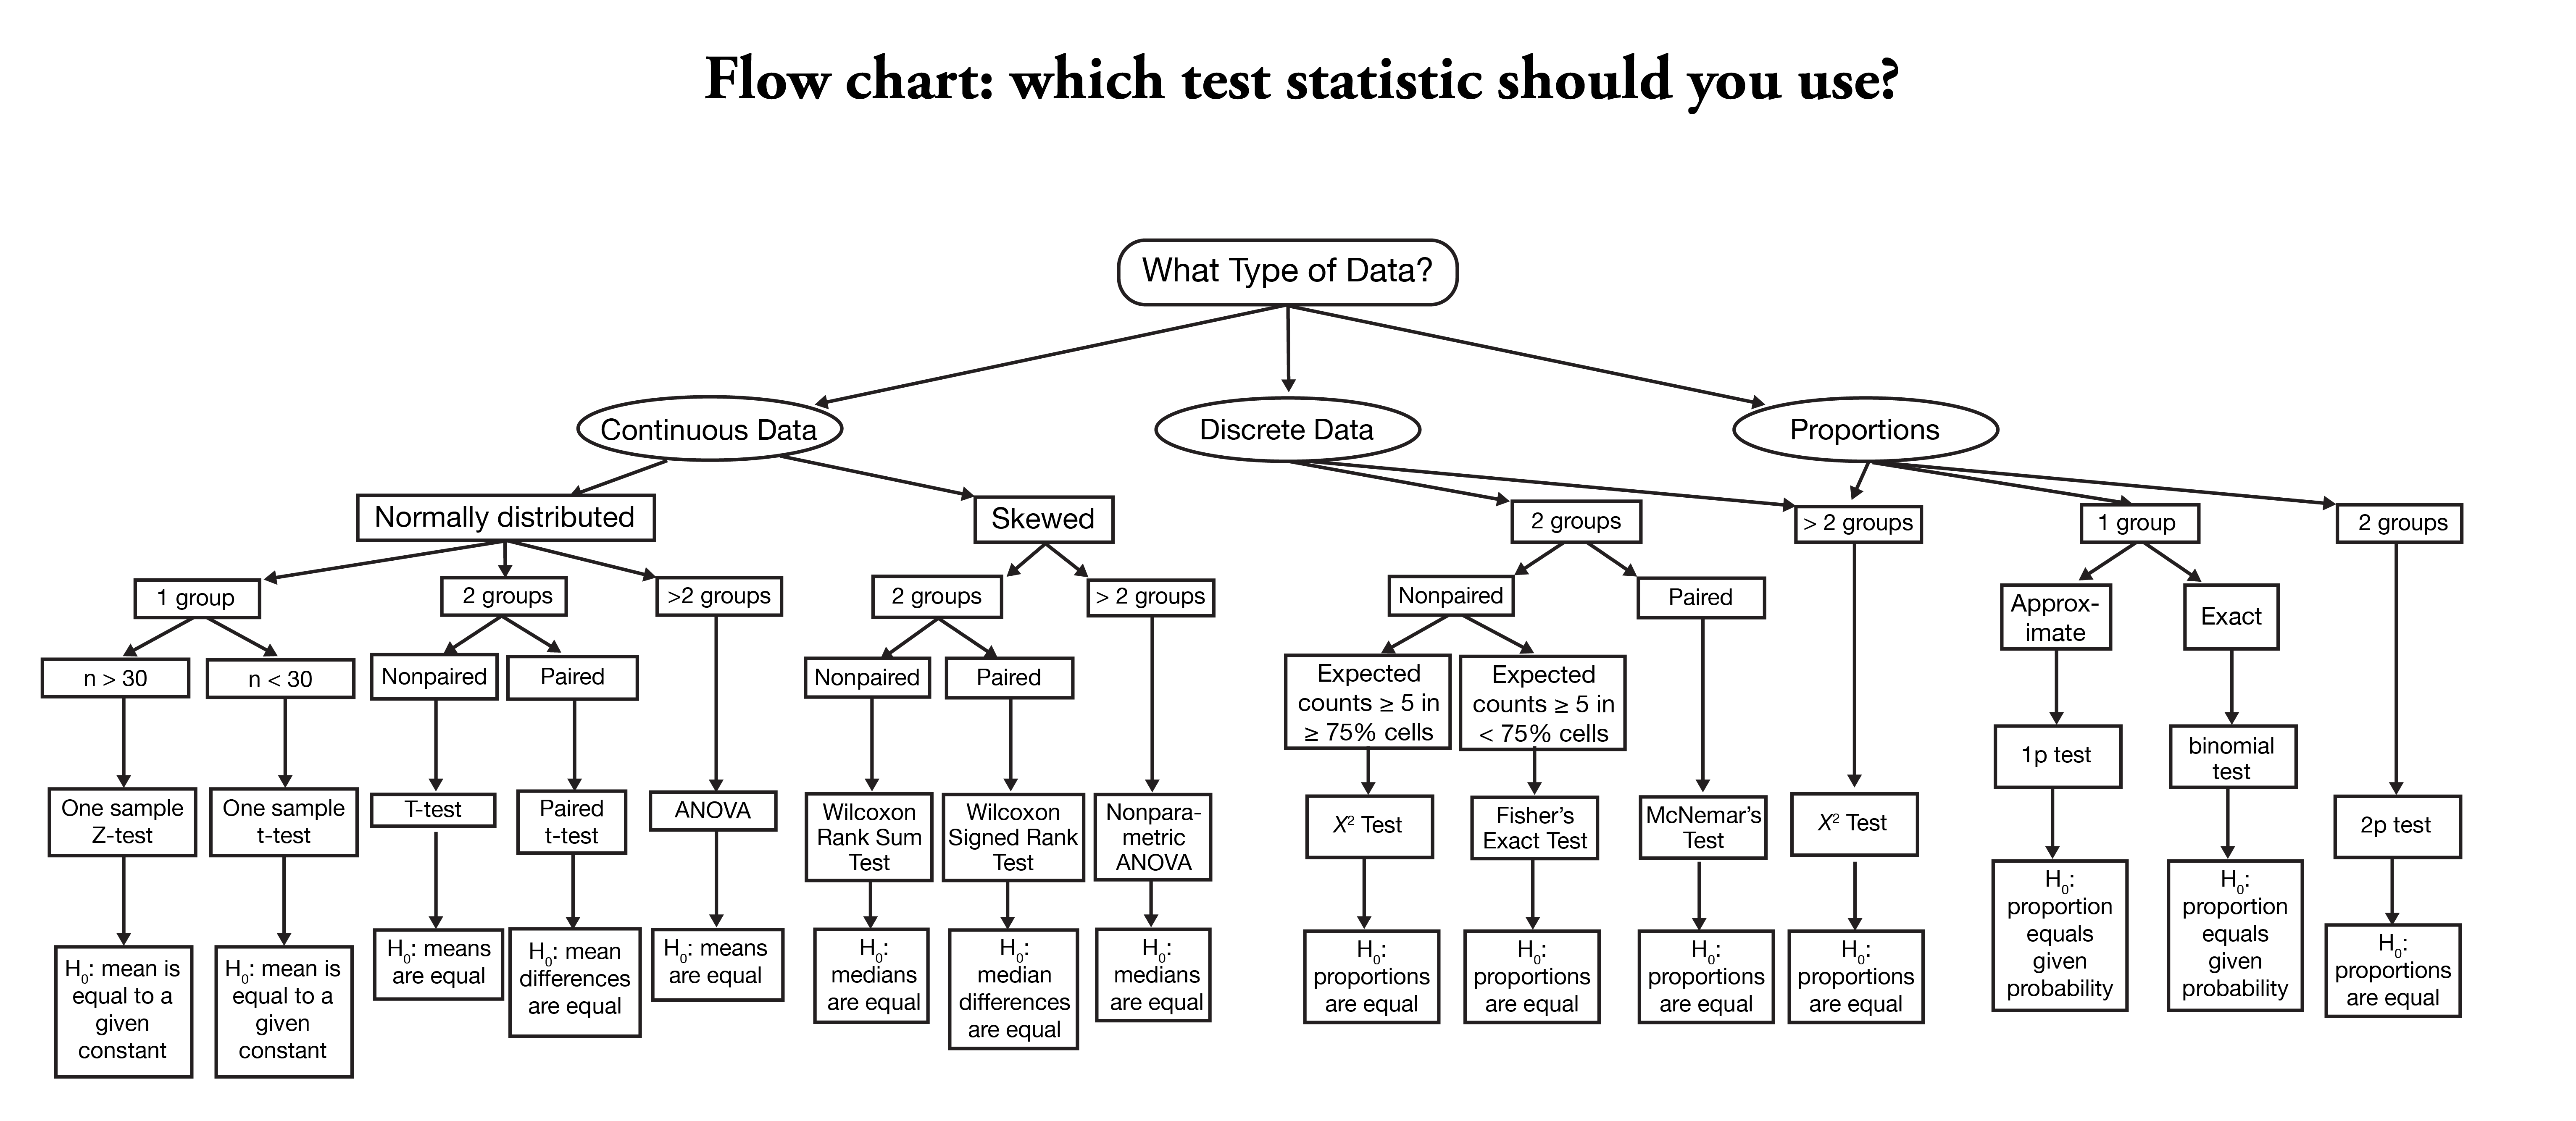
\includegraphics[keepaspectratio]{Section1/Chapter1/Pictures/which_test_flowchart.png}}}{}}\label{section-1}

\section{Different test statistics}\label{different-test-statistics}

\textbf{Chi-square test:} This test statistic is used to determine the
association between categorical dependent and categorical independent
variables. Multiple chi-square tests are used if the degree of freedom
is 1, 2, or more.

\begin{itemize}
\item
  \textbf{Pearson Chi-Square test:} It is used if the degree of freedom
  is 1 or more, variables are independent (not paired), and the expected
  cell count is \textgreater5.
\item
  \textbf{Chi-square test with Yates correction:} It is used if the
  degree of freedom is 1, variables are independent (not paired), and
  the total sample size is \textless50.
\item
  \textbf{Fischer's exact test:} It is used if the degree of freedom is
  1, variables are independent (not paired), and the expected cell count
  is \textless5.
\item
  \textbf{McNemar test:} It is used if the degree of freedom is 1, and
  variables are paired (not independent).
\end{itemize}

\textbf{Correlation:} This test statistic is used to determine the
association between two numerical dependent and independent variables.
There are two correlation coefficients calculated for two different
conditions.

\begin{enumerate}
\def\labelenumi{\arabic{enumi}.}
\item
  \textbf{Pearson's correlation:} This test statistic is used if both
  dependent and independent variables are normally distributed.
\item
  \textbf{Spearman correlation:} This test statistic is used if
  dependent or independent variables are non-normally distributed.
\end{enumerate}

\textbf{One sample Z-test:} This test is used to compare th the mean
from the sample with the hyppthesized value.

\textbf{T-test or Z-test:} These test statistics are used to compare
normally distributed means across two categories. The T-test is used if
the population variance is unknown or the sample size is small.
Otherwise, the Z test can be used.

\textbf{Paired T-test:} These test statistic is used to compare normally
distributed means between pairs.

\textbf{Mann-Whitney U Test :} It is non-parametric alternative of
T-test.

\textbf{Wilcoxon Rank-Sum Test:} It is non-parametric alternative of
paired T-test.

\textbf{ANOVA (Analysis of Variance):} Used when comparing means across
more than two groups. One-way ANOVA is used for one independent
variable, while two-way ANOVA involves two independent variables.

\textbf{Kruskal-Wallis Test:} This is a non-parametric alternative to
ANOVA, used when comparing non-normally distributed mean between three
or more independent categories.

\textbf{Repeated measure ANOVA:} This is used if the normally
distributed numeric variables are compared between three or more
measurements (repeated measure data).

\textbf{Fried Mann test:} This is used if the non-normally distributed
numeric variables are compared between three or more repeated
measurements.

\begin{tcolorbox}[enhanced jigsaw, bottomrule=.15mm, breakable, opacityback=0, toptitle=1mm, titlerule=0mm, bottomtitle=1mm, colback=white, arc=.35mm, rightrule=.15mm, toprule=.15mm, leftrule=.75mm, title=\textcolor{quarto-callout-note-color}{\faInfo}\hspace{0.5em}{Note}, colbacktitle=quarto-callout-note-color!10!white, colframe=quarto-callout-note-color-frame, coltitle=black, left=2mm, opacitybacktitle=0.6]

Always ensure that the assumptions of the chosen test are met for your
data. If you are unsure about which test statistic to use, consulting
with a statistician or using statistical software that guides you based
on your data and research question is a good practice.

\end{tcolorbox}

Before having some practical insights on using R for basic statistical
analysis, Let's explore the dataset that we will be using. In this
section, we will use the
\href{https://docs.google.com/spreadsheets/d/1I48EYm1-Sjqf6bpl86THKRZTestkz8zd/edit?usp=sharing&ouid=104920255804926220816&rtpof=true&sd=true}{WCGS
(Western Collaborative Group Study data) dataset} to demonstrate the
different basic statistical analysis. The variable names and their
description are as follows:

\begin{itemize}
\item
  \texttt{id} Subject ID:
\item
  \texttt{age} Age: age in years
\item
  \texttt{height} Height: height in inches
\item
  \texttt{weight} Weight: weight in pounds
\item
  \texttt{sbp} Systolic blood pressure: mm Hg
\item
  \texttt{dbp} Diastolic blood pressure: mm Hg
\item
  \texttt{chol} Cholesterol: mg/100 ml
\item
  \texttt{behpat} Behavior pattern:
\item
  \texttt{ncigs} Smoking: Cigarettes/day
\item
  \texttt{dibpat} Dichotomous behavior pattern: 0 = Type B; 1 = Type A
\item
  \texttt{chd69} Coronary heart disease event: 0 = none; 1 = yes
\item
  \texttt{typechd} to be done
\item
  \texttt{time169} Observation (follow up) time: Days
\item
  \texttt{arcus} Corneal arcus: 0 = none; 1 = yes
\end{itemize}

\section{Checking Assumptions}\label{checking-assumptions}

Nearly every test in this chapter comes in two ways: a
\textbf{parametric} version (assumes normally distributed data, usually
more powerful when its assumptions hold) and a \textbf{non-parametric}
version (works on ranks instead of raw values, valid under much weaker
assumptions, but somewhat less powerful when the data really are
normal). Before choosing between them, it helps to check the two
assumptions that drive that choice: \textbf{normality} and \textbf{equal
variance (homogeneity of variance)}.

\subsection{Skewness, Kurtosis and
Normality}\label{skewness-kurtosis-and-normality}

\subsubsection{Skewness and Kurtosis}\label{skewness-and-kurtosis-1}

\begin{itemize}
\tightlist
\item
  \textbf{Skewness:} Skewness measures the asymmetry of a distribution.
  It indicates whether the data is skewed to the left (negatively
  skewed) or to the right (positively skewed). A skewness value close to
  0 suggest a roughly symmetric distribution. Negative skewness
  indicates a tail to the left while positive skewness indicates a tail
  to the right
\item
  \textbf{Kurtosis:} Kurtosis measures the ``tailedness'' of a
  distribution. It reflects how much data is in the tails and how sharp
  or flat the peak is. A kurtosis value around 0 is associated to normal
  distribution. Positive kurtosis indicates heavier tails while negative
  kurtosis indicates lighter tails.
\end{itemize}

We can calculate skewness and kurtosis using \textbf{moments} package.
Lets calculate skewness and kurtosis in our dataset.

Function used: \texttt{skewness\ ()} and \texttt{kurtosis()}

\begin{Shaded}
\begin{Highlighting}[]
\CommentTok{\# install.packages("moments")}
\FunctionTok{library}\NormalTok{(moments)}

\CommentTok{\# skewness}
\FunctionTok{skewness}\NormalTok{(data}\SpecialCharTok{$}\NormalTok{age) }\CommentTok{\# Interpretation: slight right ward skew}
\end{Highlighting}
\end{Shaded}

\begin{verbatim}
#> [1] 0.5263655
\end{verbatim}

\begin{Shaded}
\begin{Highlighting}[]
\FunctionTok{kurtosis}\NormalTok{(data}\SpecialCharTok{$}\NormalTok{age) }\CommentTok{\# Interpretation: it is higher than 3 (this indicates heavier tails)}
\end{Highlighting}
\end{Shaded}

\begin{verbatim}
#> [1] 2.227403
\end{verbatim}

\pandocbounded{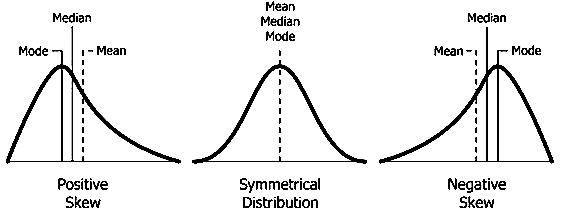
\includegraphics[keepaspectratio]{Section2/images/clipboard-69093760.png}}

\subsubsection{Testing normality of numeric
variables}\label{testing-normality-of-numeric-variables-1}

Normality is an important assumption in many statistical tests, such as
\textbf{t-tests, ANOVA, linear regression, and parametric tests}.
Ensuring that data is normally distributed helps validate the results of
these tests and ensures the reliability of statistical inferences. In
the figure below, only middle one is normally distributed whereas other
two are not.

\pandocbounded{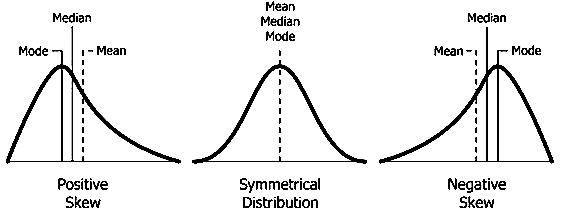
\includegraphics[keepaspectratio]{Section1/Chapter5/Pictures/skewed data.png}}

Normality testing can be conducted using several methods:

\begin{enumerate}
\def\labelenumi{\arabic{enumi}.}
\tightlist
\item
  Statistical test

  \begin{enumerate}
  \def\labelenumii{\arabic{enumii}.}
  \tightlist
  \item
    Shapiro-Wilk test
  \item
    Kolmogorov-Smirnov (KS) test
  \end{enumerate}
\item
  Graphical

  \begin{enumerate}
  \def\labelenumii{\arabic{enumii}.}
  \tightlist
  \item
    Q-Q plot
  \item
    Histogram
  \end{enumerate}
\end{enumerate}

\paragraph{Shapiro-Wilk Test}\label{shapiro-wilk-test-1}

The Shapiro-Wilk test is a widely used statistical test for normality.
It evaluates the null hypothesis that a sample comes from a normally
distributed population. It is particularly effective for small to
moderate sample sizes (typically \textless{} 50).

\textbf{Shapiro-Wilk test} (\texttt{shapiro.test()}) tests \(H_0:\) the
data are drawn from a normal distribution, vs.~\(H_1:\) they are not.
The test statistic, W, compares the observed data to what would be
expected under normality. A p-value \textless{} 0.05 often leads to
rejecting the null hypothesis, indicating non-normality.

\begin{Shaded}
\begin{Highlighting}[]
\NormalTok{dt }\OtherTok{\textless{}{-}} \FunctionTok{rnorm}\NormalTok{(}\DecValTok{1000}\NormalTok{)}

\CommentTok{\# Shapiro wilk test (works for sample \textless{}5000)}
\FunctionTok{shapiro.test}\NormalTok{(dt)}
\end{Highlighting}
\end{Shaded}

\begin{verbatim}
#> 
#>  Shapiro-Wilk normality test
#> 
#> data:  dt
#> W = 0.99825, p-value = 0.4036
\end{verbatim}

\begin{Shaded}
\begin{Highlighting}[]
\FunctionTok{shapiro.test}\NormalTok{(data}\SpecialCharTok{$}\NormalTok{height)   }\CommentTok{\# roughly symmetric, bell{-}shaped variable}
\end{Highlighting}
\end{Shaded}

\begin{verbatim}
#> 
#>  Shapiro-Wilk normality test
#> 
#> data:  data$height
#> W = 0.98357, p-value < 2.2e-16
\end{verbatim}

\begin{Shaded}
\begin{Highlighting}[]
\FunctionTok{shapiro.test}\NormalTok{(data}\SpecialCharTok{$}\NormalTok{ncigs)    }\CommentTok{\# heavily right{-}skewed (many non{-}smokers {-}\textgreater{} many zeros)}
\end{Highlighting}
\end{Shaded}

\begin{verbatim}
#> 
#>  Shapiro-Wilk normality test
#> 
#> data:  data$ncigs
#> W = 0.78164, p-value < 2.2e-16
\end{verbatim}

\begin{tcolorbox}[enhanced jigsaw, bottomrule=.15mm, breakable, opacityback=0, toptitle=1mm, titlerule=0mm, bottomtitle=1mm, colback=white, arc=.35mm, rightrule=.15mm, toprule=.15mm, leftrule=.75mm, title=\textcolor{quarto-callout-caution-color}{\faFire}\hspace{0.5em}{Caution}, colbacktitle=quarto-callout-caution-color!10!white, colframe=quarto-callout-caution-color-frame, coltitle=black, left=2mm, opacitybacktitle=0.6]

Shapiro-Wilk (like most goodness-of-fit tests) becomes extremely
sensitive with large samples in a cohort of 3154 like \texttt{wcgs},
even trivial, practically unimportant deviations from normality will
produce a significant (p \textless{} 0.05) result. For large \(n\),
weigh the Q-Q plot and histogram more heavily than the p-value alone,
and rely on the Central Limit Theorem (sample means are approximately
normal for large \(n\) even when the raw data are not) when deciding
whether a t-test/ANOVA is still reasonable.

\end{tcolorbox}

\textbf{Interpretation:} The test statistic (W) is 0.99786, and the
p-value is 0.7844. With a high p-value, there is no significant evidence
to reject the null hypothesis, suggesting that the data is reasonably
consistent with a normal distribution.

\paragraph{Kolmogorov-Smirnov (KS)
test}\label{kolmogorov-smirnov-ks-test-1}

The Kolmogorov-Smirnov test is a non-parametric test used to compare a
sample distribution to a reference distribution (e.g., normal
distribution). It measures the maximum distance between the empirical
distribution function of the sample and the cumulative distribution
function of the reference distribution. While it can be used for
normality testing, it is less powerful than the Shapiro-Wilk test for
this purpose, especially for small samples.

\begin{Shaded}
\begin{Highlighting}[]
\CommentTok{\# KS test}
\FunctionTok{ks.test}\NormalTok{(dt,}\StringTok{"pnorm"}\NormalTok{, }\AttributeTok{exact =}\NormalTok{ T)}
\end{Highlighting}
\end{Shaded}

\begin{verbatim}
#> 
#>  Exact one-sample Kolmogorov-Smirnov test
#> 
#> data:  dt
#> D = 0.030564, p-value = 0.3015
#> alternative hypothesis: two-sided
\end{verbatim}

\textbf{Interpretation:} The test statistic (D) is 0.017067, and the
p-value is 0.9982. With a high p-value, there is no significant evidence
to reject the null hypothesis, indicating that the data does not
significantly differ from the assumed distribution in a two-sided test.

\paragraph{Q-Q plot}\label{q-q-plot-1}

A Q-Q plot is a graphical tool to assess whether a dataset follows a
particular distribution, such as the normal distribution. It plots the
quantiles of the sample data against the quantiles of the theoretical
distribution. If the points fall approximately along a straight line,
the data is likely normally distributed. Deviations from the line (e.g.,
curves or outliers) suggest departures from normality.

\begin{Shaded}
\begin{Highlighting}[]
\CommentTok{\# QQ plot}
\FunctionTok{qqnorm}\NormalTok{(data}\SpecialCharTok{$}\NormalTok{age)}
\end{Highlighting}
\end{Shaded}

\begin{center}
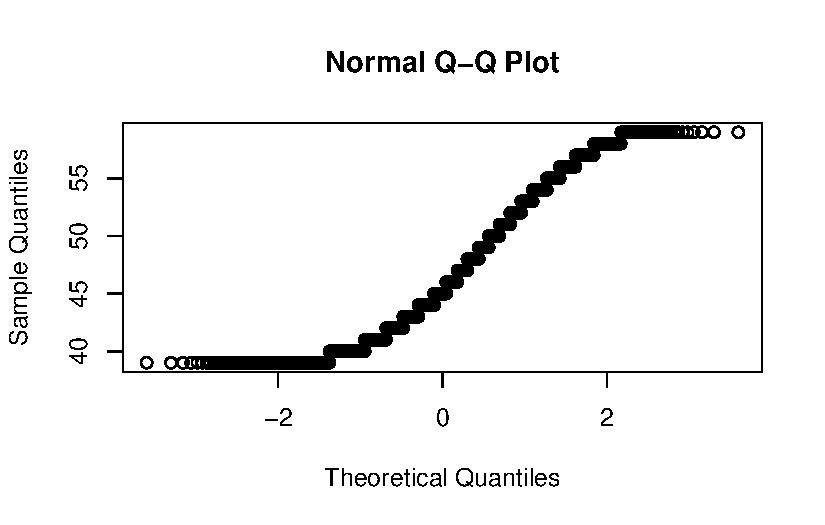
\includegraphics[width=0.85\linewidth,height=\textheight,keepaspectratio]{Section2/05_bivariate_files/figure-pdf/unnamed-chunk-6-1.pdf}
\end{center}

\textbf{Interpretation:} In the first chart, the points do not deviate
significantly from the line, indicating that the data, \texttt{dt}, is
normally distributed. However, in the second chart, the points deviate
from the line, forming an S-shaped curve, which suggests that the data
is not normally distributed.

\paragraph{Histogram}\label{histogram-2}

A histogram is a visual representation of the distribution of a dataset.
It divides the data into bins and displays the frequency of observations
in each bin.For normality testing, the shape of the histogram is
compared to the bell-shaped curve of a normal distribution. Symmetry,
peak at the mean, and tapering tails are indicators of normality. While
useful for a quick visual check, histograms can be subjective and less
reliable for small sample sizes.

\begin{Shaded}
\begin{Highlighting}[]
\CommentTok{\# Histogram}
\NormalTok{sequence }\OtherTok{\textless{}{-}} \FunctionTok{seq}\NormalTok{(}\FunctionTok{min}\NormalTok{(data}\SpecialCharTok{$}\NormalTok{age), }\FunctionTok{max}\NormalTok{(data}\SpecialCharTok{$}\NormalTok{age), }\DecValTok{1}\NormalTok{)}
\NormalTok{fun }\OtherTok{\textless{}{-}} \FunctionTok{dnorm}\NormalTok{(sequence, }\AttributeTok{mean =} \FunctionTok{mean}\NormalTok{(data}\SpecialCharTok{$}\NormalTok{age), }\AttributeTok{sd =} \FunctionTok{sd}\NormalTok{(data}\SpecialCharTok{$}\NormalTok{age))}
\FunctionTok{hist}\NormalTok{(data}\SpecialCharTok{$}\NormalTok{age,}
     \AttributeTok{main =} \StringTok{"data"}\NormalTok{,}
     \AttributeTok{ylab =} \StringTok{"Frequency"}\NormalTok{,}
     \AttributeTok{xlab=}\StringTok{"dt"}\NormalTok{,}
     \AttributeTok{col=}\StringTok{"skyblue"}\NormalTok{, }\AttributeTok{probability =}\NormalTok{ T)}
\FunctionTok{lines}\NormalTok{(sequence, fun, }\AttributeTok{col=}\StringTok{"blue"}\NormalTok{, }\AttributeTok{lwd=}\DecValTok{2}\NormalTok{)}
\end{Highlighting}
\end{Shaded}

\begin{center}
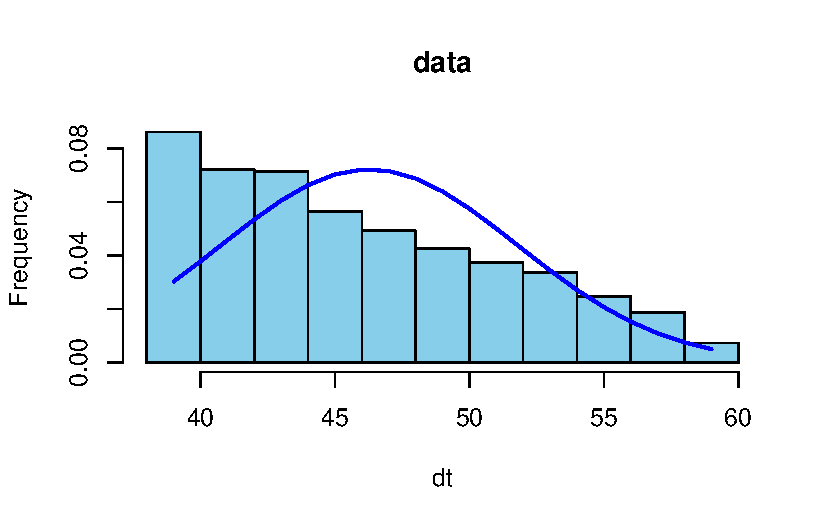
\includegraphics[width=0.85\linewidth,height=\textheight,keepaspectratio]{Section2/05_bivariate_files/figure-pdf/unnamed-chunk-7-1.pdf}
\end{center}

\textbf{Interpretation:} Since, the chart seems to be asymmetric which
indicates that the data is not normally distributed.

\subsection{Equal Variance (Homogeneity of
Variance)}\label{equal-variance-homogeneity-of-variance}

Two-sample and multi-group tests often additionally assume the groups
being compared have similar variances. Three common formal tests:

\begin{itemize}
\tightlist
\item
  \textbf{F-test for two variances} (\texttt{var.test()}): compares the
  variances of exactly two groups; assumes each group is itself normally
  distributed.
\item
  \textbf{Bartlett's test} (\texttt{bartlett.test()}): generalizes the
  F-test to two or more groups; also assumes normality within each
  group.
\item
  \textbf{Levene's test} (\texttt{car::leveneTest()}): tests the same
  hypothesis as Bartlett's test but is \textbf{robust to non-normality},
  making it the preferred default in practice.
\end{itemize}

\begin{Shaded}
\begin{Highlighting}[]
\FunctionTok{var.test}\NormalTok{(chol }\SpecialCharTok{\textasciitilde{}}\NormalTok{ chd69, }\AttributeTok{data =}\NormalTok{ data)                    }\CommentTok{\# two groups only}
\end{Highlighting}
\end{Shaded}

\begin{verbatim}
#> 
#>  F test to compare two variances
#> 
#> data:  chol by chd69
#> F = 0.73046, num df = 2884, denom df = 256, p-value = 0.0003389
#> alternative hypothesis: true ratio of variances is not equal to 1
#> 95 percent confidence interval:
#>  0.6052449 0.8694154
#> sample estimates:
#> ratio of variances 
#>          0.7304583
\end{verbatim}

\begin{Shaded}
\begin{Highlighting}[]
\FunctionTok{bartlett.test}\NormalTok{(chol }\SpecialCharTok{\textasciitilde{}}\NormalTok{ agec, }\AttributeTok{data =}\NormalTok{ data)                 }\CommentTok{\# \textgreater{}= 2 groups, assumes normal within each}
\end{Highlighting}
\end{Shaded}

\begin{verbatim}
#> 
#>  Bartlett test of homogeneity of variances
#> 
#> data:  chol by agec
#> Bartlett's K-squared = 11.227, df = 4, p-value = 0.02413
\end{verbatim}

\begin{Shaded}
\begin{Highlighting}[]
\NormalTok{car}\SpecialCharTok{::}\FunctionTok{leveneTest}\NormalTok{(chol }\SpecialCharTok{\textasciitilde{}} \FunctionTok{factor}\NormalTok{(agec), }\AttributeTok{data =}\NormalTok{ data)        }\CommentTok{\# \textgreater{}= 2 groups, robust to non{-}normality}
\end{Highlighting}
\end{Shaded}

\begin{verbatim}
#> Levene's Test for Homogeneity of Variance (center = median)
#>         Df F value Pr(>F)
#> group    4  0.3182  0.866
#>       3137
\end{verbatim}

For all three, \(H_0:\) the group variances are equal, vs.~\(H_1:\) they
are not. A significant result (p \textless{} 0.05) means the
equal-variance assumption is violated, and a variance-robust version of
the downstream test (Welch's t-test, Welch's ANOVA --- both covered
below) should be used instead of the classic (equal-variance) version.

\section{Decision Summary}\label{decision-summary}

\begin{longtable}[]{@{}
  >{\raggedright\arraybackslash}p{(\linewidth - 4\tabcolsep) * \real{0.3333}}
  >{\raggedright\arraybackslash}p{(\linewidth - 4\tabcolsep) * \real{0.3333}}
  >{\raggedright\arraybackslash}p{(\linewidth - 4\tabcolsep) * \real{0.3333}}@{}}
\toprule\noalign{}
\begin{minipage}[b]{\linewidth}\raggedright
Question
\end{minipage} & \begin{minipage}[b]{\linewidth}\raggedright
Test to use if assumption holds
\end{minipage} & \begin{minipage}[b]{\linewidth}\raggedright
Test to use if normality assumption is violated
\end{minipage} \\
\midrule\noalign{}
\endhead
\bottomrule\noalign{}
\endlastfoot
Association between two numeric variables & Pearson correlation
coefficient & Spearman rank correlation coefficient \\
Compare 1 sample mean to a fixed value & One-sample t-test (or z-test if
\(\sigma\) known) & Wilcoxon signed-rank test \\
Compare 2 independent group means & Student's t-test (equal variance) &
Welch's t-test (unequal variance) or Mann-Whitney U (non-normal) \\
Compare paired/matched measurements & Paired t-test & Wilcoxon
signed-rank test \\
Compare 3+ independent group means & One-way ANOVA & Welch's ANOVA
(unequal variance) or Kruskal-Wallis (non-normal) \\
Compare 3+ repeated/matched measurements & Repeated-measures ANOVA &
Friedman test \\
Association between two independent categorical variables & & Chi-square
test \\
Association between two dependent categorical variables & & McNemar
Chi-square test \\
\end{longtable}

\section{\texorpdfstring{\textbf{Association between two numeric
variables}}{Association between two numeric variables}}\label{association-between-two-numeric-variables}

\section{Correlation}\label{correlation}

Correlation is used to measure the \textbf{strength and direction of
association between two numerical variables}. A \textbf{scatter plot}
ideally comes immediately before correlation tests because it helps
readers visually understand what correlation is measuring.The
correlation coefficient is scale-free, meaning that it does not depend
on the measurement units of the variables. It can be \textbf{Pearson
correlation coefficient} or \textbf{Spearman rank correlation
coefficient}.

The \textbf{Pearson correlation coefficient} is commonly used when both
variables are continuous and the relationship between them is
approximately linear, with no substantial influence from extreme
outliers. The \textbf{Spearman rank correlation coefficient} is a
nonparametric measure that is appropriate when the assumptions required
for Pearson correlation are not satisfied, particularly when the
variables are ordinal, substantially skewed, affected by outliers, or
when the relationship is monotonic but not necessarily linear.

Therefore, the choice between Pearson and Spearman correlation is based
on the characteristics of the data and the assumptions of the analysis
rather than simply labeling a variable as parametric or nonparametric.

In WCGS dataset, lets determine association between age and systolic
blood pressure

\begin{Shaded}
\begin{Highlighting}[]
\CommentTok{\#lets plot a chart}
\FunctionTok{plot}\NormalTok{(data}\SpecialCharTok{$}\NormalTok{age, data}\SpecialCharTok{$}\NormalTok{sbp) }\CommentTok{\# plot scatterplot}
\end{Highlighting}
\end{Shaded}

\begin{center}
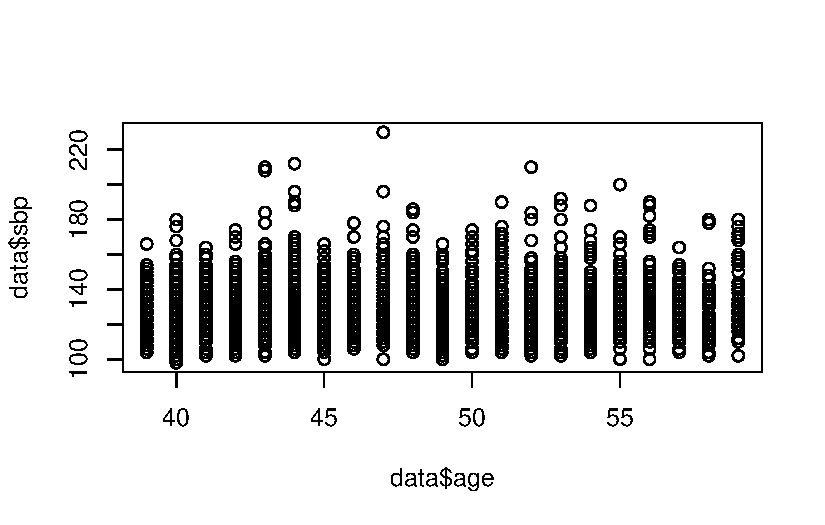
\includegraphics[width=0.85\linewidth,height=\textheight,keepaspectratio]{Section2/05_bivariate_files/figure-pdf/unnamed-chunk-9-1.pdf}
\end{center}

\begin{Shaded}
\begin{Highlighting}[]
\FunctionTok{hist}\NormalTok{(data}\SpecialCharTok{$}\NormalTok{age) }\CommentTok{\# plot histogram for age}
\end{Highlighting}
\end{Shaded}

\begin{center}
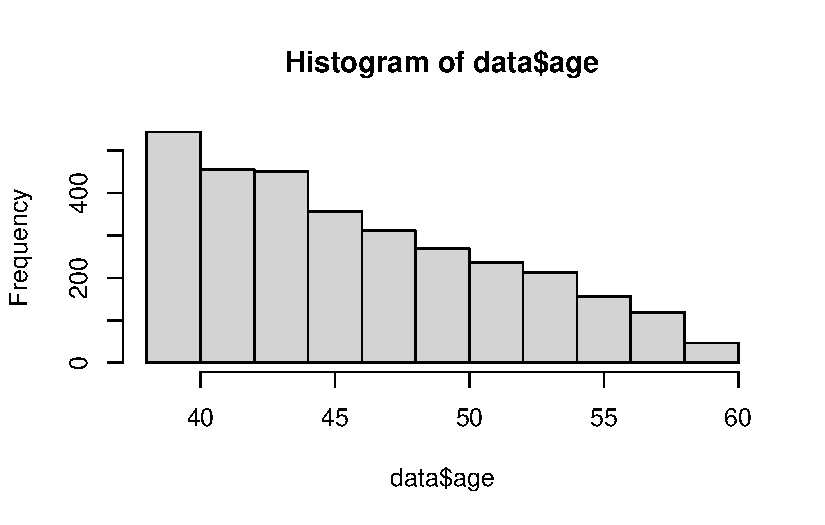
\includegraphics[width=0.85\linewidth,height=\textheight,keepaspectratio]{Section2/05_bivariate_files/figure-pdf/unnamed-chunk-9-2.pdf}
\end{center}

\begin{Shaded}
\begin{Highlighting}[]
\FunctionTok{qqnorm}\NormalTok{(data}\SpecialCharTok{$}\NormalTok{age) }\CommentTok{\#check normality of the age}
\end{Highlighting}
\end{Shaded}

\begin{center}
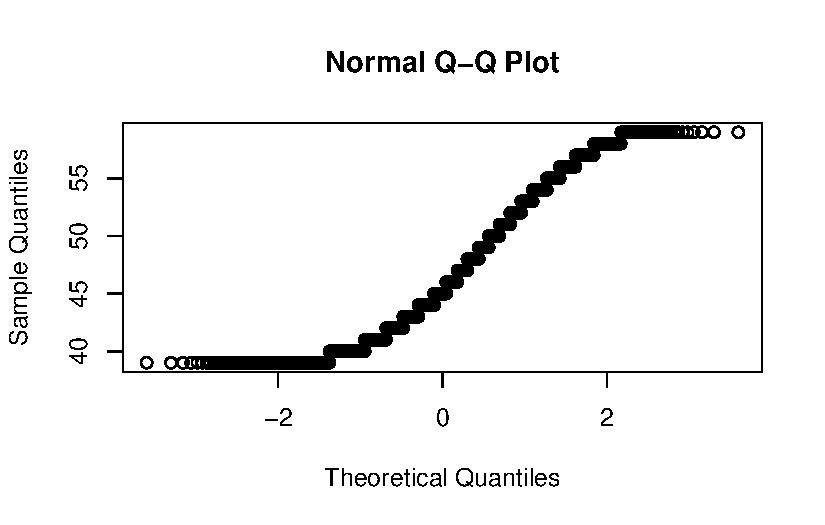
\includegraphics[width=0.85\linewidth,height=\textheight,keepaspectratio]{Section2/05_bivariate_files/figure-pdf/unnamed-chunk-9-3.pdf}
\end{center}

\begin{Shaded}
\begin{Highlighting}[]
\FunctionTok{shapiro.test}\NormalTok{(data}\SpecialCharTok{$}\NormalTok{age) }\CommentTok{\# formal normality test}
\end{Highlighting}
\end{Shaded}

\begin{verbatim}
#> 
#>  Shapiro-Wilk normality test
#> 
#> data:  data$age
#> W = 0.93589, p-value < 2.2e-16
\end{verbatim}

\begin{Shaded}
\begin{Highlighting}[]
\FunctionTok{hist}\NormalTok{(data}\SpecialCharTok{$}\NormalTok{sbp)  }\CommentTok{\# plot histogram for systolic bp}
\end{Highlighting}
\end{Shaded}

\begin{center}
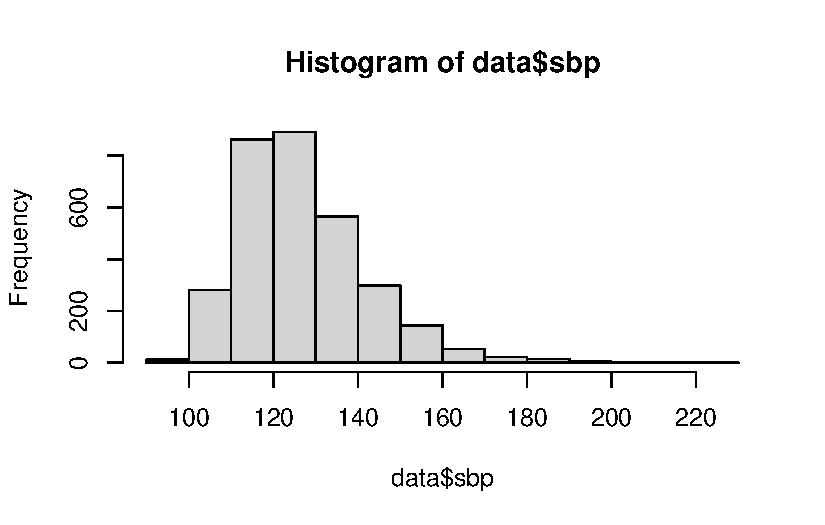
\includegraphics[width=0.85\linewidth,height=\textheight,keepaspectratio]{Section2/05_bivariate_files/figure-pdf/unnamed-chunk-9-4.pdf}
\end{center}

\begin{Shaded}
\begin{Highlighting}[]
\FunctionTok{qqnorm}\NormalTok{(data}\SpecialCharTok{$}\NormalTok{sbp) }\CommentTok{\#check normality of systolic bp}
\end{Highlighting}
\end{Shaded}

\begin{center}
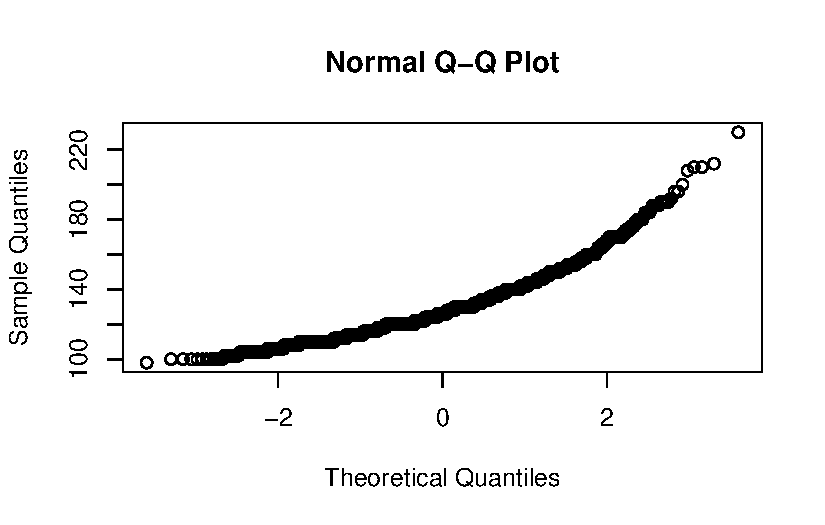
\includegraphics[width=0.85\linewidth,height=\textheight,keepaspectratio]{Section2/05_bivariate_files/figure-pdf/unnamed-chunk-9-5.pdf}
\end{center}

\begin{Shaded}
\begin{Highlighting}[]
\FunctionTok{shapiro.test}\NormalTok{(data}\SpecialCharTok{$}\NormalTok{sbp) }\CommentTok{\# formal normality test}
\end{Highlighting}
\end{Shaded}

\begin{verbatim}
#> 
#>  Shapiro-Wilk normality test
#> 
#> data:  data$sbp
#> W = 0.93218, p-value < 2.2e-16
\end{verbatim}

\begin{Shaded}
\begin{Highlighting}[]
\FunctionTok{cor.test}\NormalTok{(data}\SpecialCharTok{$}\NormalTok{age, data}\SpecialCharTok{$}\NormalTok{sbp,}\AttributeTok{method=}\StringTok{"spearman"}\NormalTok{) }\CommentTok{\# if they were parametric you would have write "pearson" instead of "spearman"}
\end{Highlighting}
\end{Shaded}

\begin{verbatim}
#> 
#>  Spearman's rank correlation rho
#> 
#> data:  data$age and data$sbp
#> S = 4395383487, p-value < 2.2e-16
#> alternative hypothesis: true rho is not equal to 0
#> sample estimates:
#>       rho 
#> 0.1594511
\end{verbatim}

\section{Compare one sample mean with fixed
value}\label{compare-one-sample-mean-with-fixed-value}

\subsection{One-Sample Tests}\label{one-sample-tests}

A one-sample test compares a single sample's central tendency to a
fixed, hypothesized value.

\textbf{One-Sample Z-test vs.~One-Sample T-test}

\[ Z_{stat}=\frac{\bar x-\mu_0}{\sigma/\sqrt n} \qquad\qquad t_{stat}=\frac{\bar x-\mu_0}{s/\sqrt n},\; df=n-1 \]

The \textbf{z-test} requires the population standard deviation
\(\sigma\) to be known in advance --- rare in practice, since if we
don't know the population mean we usually don't know its standard
deviation either. The \textbf{t-test} instead estimates \(\sigma\) from
the sample (\(s\)) and uses the (slightly wider, more conservative)
\(t\)-distribution with \(n-1\) degrees of freedom to account for that
extra estimation uncertainty. As \(n\) grows large, the
\(t\)-distribution converges to the normal (z) distribution, so the two
tests give nearly identical results for large samples.

\begin{Shaded}
\begin{Highlighting}[]
\CommentTok{\# One{-}sample t{-}test: is average cholesterol in this cohort different from a reference value of 220?}
\FunctionTok{t.test}\NormalTok{(data}\SpecialCharTok{$}\NormalTok{chol, }\AttributeTok{mu =} \DecValTok{220}\NormalTok{)}
\end{Highlighting}
\end{Shaded}

\begin{verbatim}
#> 
#>  One Sample t-test
#> 
#> data:  data$chol
#> t = 8.2264, df = 3141, p-value = 2.793e-16
#> alternative hypothesis: true mean is not equal to 220
#> 95 percent confidence interval:
#>  224.8536 227.8912
#> sample estimates:
#> mean of x 
#>  226.3724
\end{verbatim}

\begin{Shaded}
\begin{Highlighting}[]
\CommentTok{\# One{-}sample z{-}test (sigma assumed known from prior literature, e.g. sigma = 45): manual calculation,}
\CommentTok{\# since base R does not include a dedicated one{-}sample z{-}test function}
\NormalTok{xbar }\OtherTok{\textless{}{-}} \FunctionTok{mean}\NormalTok{(data}\SpecialCharTok{$}\NormalTok{chol); n }\OtherTok{\textless{}{-}} \FunctionTok{length}\NormalTok{(data}\SpecialCharTok{$}\NormalTok{chol); sigma0 }\OtherTok{\textless{}{-}} \DecValTok{45}\NormalTok{; mu0 }\OtherTok{\textless{}{-}} \DecValTok{220}
\NormalTok{z\_stat }\OtherTok{\textless{}{-}}\NormalTok{ (xbar }\SpecialCharTok{{-}}\NormalTok{ mu0) }\SpecialCharTok{/}\NormalTok{ (sigma0 }\SpecialCharTok{/} \FunctionTok{sqrt}\NormalTok{(n))}
\NormalTok{p\_val  }\OtherTok{\textless{}{-}} \DecValTok{2} \SpecialCharTok{*} \FunctionTok{pnorm}\NormalTok{(}\SpecialCharTok{{-}}\FunctionTok{abs}\NormalTok{(z\_stat))}
\FunctionTok{c}\NormalTok{(}\AttributeTok{z =}\NormalTok{ z\_stat, }\AttributeTok{p\_value =}\NormalTok{ p\_val)}
\end{Highlighting}
\end{Shaded}

\begin{verbatim}
#>       z p_value 
#>      NA      NA
\end{verbatim}

\begin{tcolorbox}[enhanced jigsaw, bottomrule=.15mm, breakable, opacityback=0, toptitle=1mm, titlerule=0mm, bottomtitle=1mm, colback=white, arc=.35mm, rightrule=.15mm, toprule=.15mm, leftrule=.75mm, title=\textcolor{quarto-callout-note-color}{\faInfo}\hspace{0.5em}{Note}, colbacktitle=quarto-callout-note-color!10!white, colframe=quarto-callout-note-color-frame, coltitle=black, left=2mm, opacitybacktitle=0.6]

\textbf{Five-step hypothesis-testing format:}

\textbf{Step 1:} State hypothesis

\(H_0:\mu=220\) vs.~\(H_1:\mu\ne220\);

\textbf{Step-2:} Level of significance

\(\alpha=0.05\)

\textbf{Step-3:} Determine test statistics

Obtain the t- (or z-) statistic and df from \texttt{t.test()}

Step-4: Read off the p-value or critical value

\textbf{Step-5:} Decision and conclusion

If p-value is less than 0.05 reject \(H_0\) and else accept \(H_0\).
Finally state the conclusion in context.

\end{tcolorbox}

\subsection{One-Sample Wilcoxon Signed-Rank Test (Non-Parametric
Alternative)}\label{one-sample-wilcoxon-signed-rank-test-non-parametric-alternative}

When the one-sample data are not (even approximately) normally
distributed and the sample is small, the \textbf{Wilcoxon signed-rank
test} replaces the one-sample t-test. Rather than working with the raw
values, it ranks the absolute deviations from the hypothesized value
\(\mu_0\) and tests whether the signed ranks are symmetric around zero,
it tests the \textbf{median}, not the mean.

\begin{Shaded}
\begin{Highlighting}[]
\FunctionTok{wilcox.test}\NormalTok{(data}\SpecialCharTok{$}\NormalTok{ncigs, }\AttributeTok{mu =} \DecValTok{5}\NormalTok{)   }\CommentTok{\# ncigs is heavily skewed {-}{-} median{-}based test is more appropriate}
\end{Highlighting}
\end{Shaded}

\begin{verbatim}
#> 
#>  Wilcoxon signed rank test with continuity correction
#> 
#> data:  data$ncigs
#> V = 3331510, p-value < 2.2e-16
#> alternative hypothesis: true location is not equal to 5
\end{verbatim}

\section{Compare two means}\label{compare-two-means}

\subsection{Two-Independent Sample tests (Parametric
test)}\label{two-independent-sample-tests-parametric-test}

This setting compares a continuous outcome between two \emph{unrelated}
groups --- for example, cholesterol between participants with and
without coronary heart disease.

\subsection{Student's T-test vs.~Welch's
T-test}\label{students-t-test-vs.-welchs-t-test}

\[ t_{stat}=\frac{\bar x_1-\bar x_2}{s_p\sqrt{\tfrac1{n_1}+\tfrac1{n_2}}},\; s_p^2=\frac{(n_1-1)s_1^2+(n_2-1)s_2^2}{n_1+n_2-2}\; (\text{Student's, assumes equal variance}) \]

\[ t_{stat}=\frac{\bar x_1-\bar x_2}{\sqrt{\tfrac{s_1^2}{n_1}+\tfrac{s_2^2}{n_2}}}\; (\text{Welch's, does not assume equal variance; df approximated by the Welch-Satterthwaite equation}) \]

\textbf{Student's t-test} pools the two groups' variances into a single
common estimate \(s_p^2\) and assumes the two population variances are
equal (check first with \texttt{var.test()} or
\texttt{car::leveneTest()}). \textbf{Welch's t-test} does not pool
variances and instead uses each group's own variance separately, with an
adjusted (often non-integer) degrees of freedom --- this makes it valid
whether or not the variances are equal, which is why \textbf{R's
\texttt{t.test()} defaults to Welch's version}
(\texttt{var.equal\ =\ FALSE}) unless told otherwise.

\begin{Shaded}
\begin{Highlighting}[]
\CommentTok{\# Check the equal{-}variance assumption first}
\FunctionTok{var.test}\NormalTok{(chol }\SpecialCharTok{\textasciitilde{}}\NormalTok{ chd69, }\AttributeTok{data =}\NormalTok{ data)}
\end{Highlighting}
\end{Shaded}

\begin{verbatim}
#> 
#>  F test to compare two variances
#> 
#> data:  chol by chd69
#> F = 0.73046, num df = 2884, denom df = 256, p-value = 0.0003389
#> alternative hypothesis: true ratio of variances is not equal to 1
#> 95 percent confidence interval:
#>  0.6052449 0.8694154
#> sample estimates:
#> ratio of variances 
#>          0.7304583
\end{verbatim}

\begin{Shaded}
\begin{Highlighting}[]
\CommentTok{\# Lets compare cholesterol level between participants with and without coronary heart disease}
\FunctionTok{qqnorm}\NormalTok{(data}\SpecialCharTok{$}\NormalTok{chol)}
\end{Highlighting}
\end{Shaded}

\begin{center}
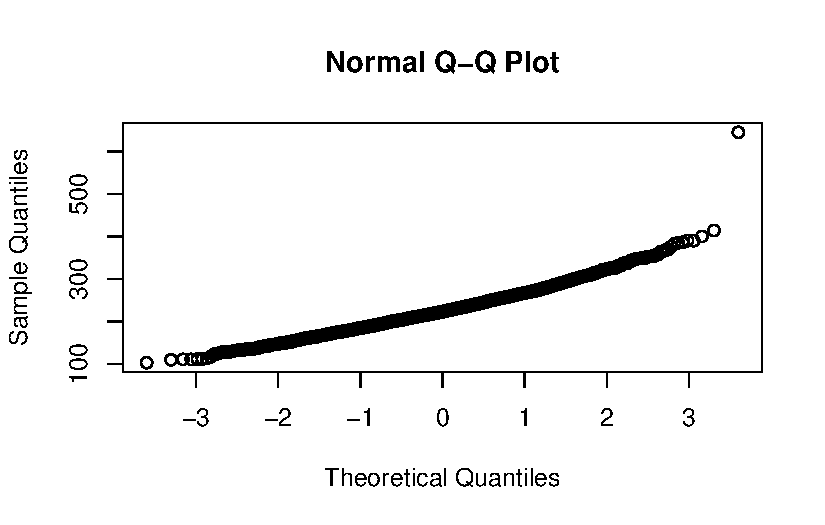
\includegraphics[width=0.85\linewidth,height=\textheight,keepaspectratio]{Section2/05_bivariate_files/figure-pdf/unnamed-chunk-12-1.pdf}
\end{center}

\begin{Shaded}
\begin{Highlighting}[]
\FunctionTok{hist}\NormalTok{(data}\SpecialCharTok{$}\NormalTok{chol)}
\end{Highlighting}
\end{Shaded}

\begin{center}
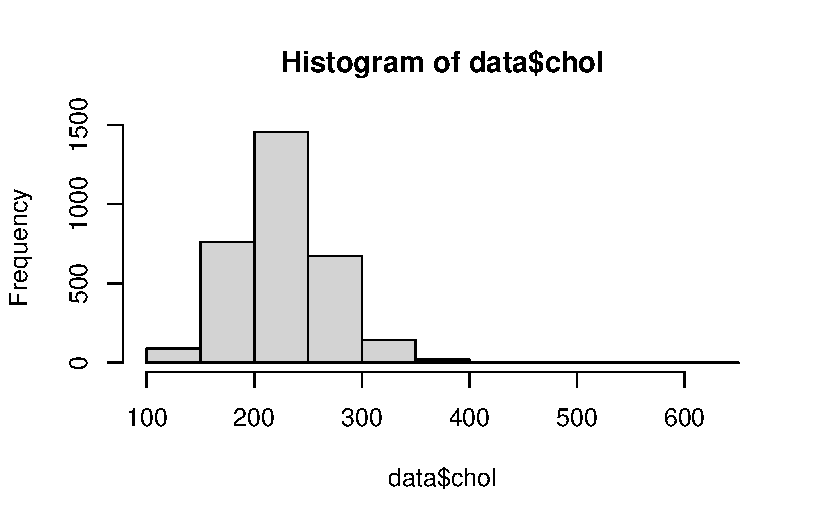
\includegraphics[width=0.85\linewidth,height=\textheight,keepaspectratio]{Section2/05_bivariate_files/figure-pdf/unnamed-chunk-12-2.pdf}
\end{center}

\begin{Shaded}
\begin{Highlighting}[]
\FunctionTok{boxplot}\NormalTok{(data}\SpecialCharTok{$}\NormalTok{chol}\SpecialCharTok{\textasciitilde{}}\NormalTok{data}\SpecialCharTok{$}\NormalTok{chd69)}
\end{Highlighting}
\end{Shaded}

\begin{center}
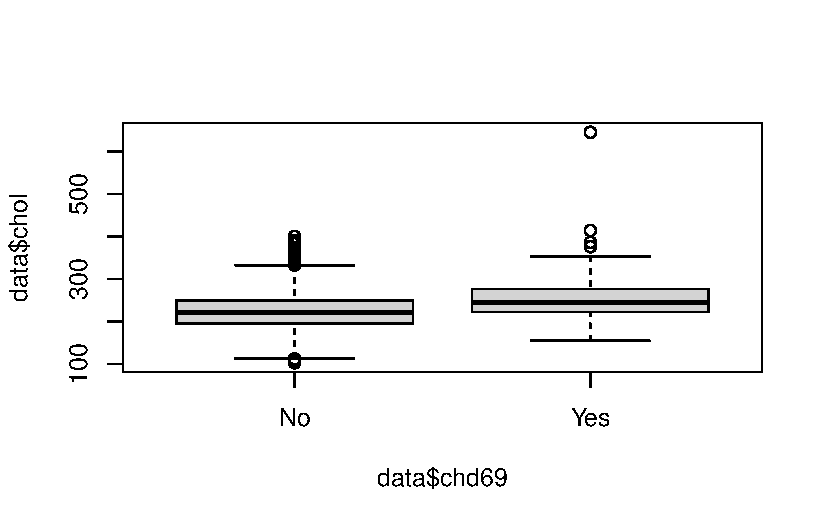
\includegraphics[width=0.85\linewidth,height=\textheight,keepaspectratio]{Section2/05_bivariate_files/figure-pdf/unnamed-chunk-12-3.pdf}
\end{center}

\begin{Shaded}
\begin{Highlighting}[]
\FunctionTok{t.test}\NormalTok{(chol}\SpecialCharTok{\textasciitilde{}}\NormalTok{chd69, }\AttributeTok{data=}\NormalTok{data,}\AttributeTok{conf=}\FloatTok{0.99}\NormalTok{)                     }\CommentTok{\# Welch\textquotesingle{}s t{-}test (R default)}
\end{Highlighting}
\end{Shaded}

\begin{verbatim}
#> 
#>  Welch Two Sample t-test
#> 
#> data:  chol by chd69
#> t = -8.1163, df = 290.29, p-value = 1.377e-14
#> alternative hypothesis: true difference in means between group No and group Yes is not equal to 0
#> 99 percent confidence interval:
#>  -34.05369 -17.56368
#> sample estimates:
#>  mean in group No mean in group Yes 
#>          224.2614          250.0700
\end{verbatim}

\begin{Shaded}
\begin{Highlighting}[]
\FunctionTok{t.test}\NormalTok{(chol}\SpecialCharTok{\textasciitilde{}}\NormalTok{chd69, }\AttributeTok{data=}\NormalTok{data, }\AttributeTok{conf=}\FloatTok{0.99}\NormalTok{, }\AttributeTok{var.equal =} \ConstantTok{TRUE}\NormalTok{)   }\CommentTok{\# Student\textquotesingle{}s t{-}test (equal{-}variance assumed)}
\end{Highlighting}
\end{Shaded}

\begin{verbatim}
#> 
#>  Two Sample t-test
#> 
#> data:  chol by chd69
#> t = -9.253, df = 3140, p-value < 2.2e-16
#> alternative hypothesis: true difference in means between group No and group Yes is not equal to 0
#> 99 percent confidence interval:
#>  -32.99765 -18.61972
#> sample estimates:
#>  mean in group No mean in group Yes 
#>          224.2614          250.0700
\end{verbatim}

\subsection{\texorpdfstring{Effect Size: Cohen's
\emph{d}}{Effect Size: Cohen's d}}\label{effect-size-cohens-d}

A p-value only indicates whether a difference is \emph{statistically
detectable}; it says nothing about how \emph{large} the difference is.
\textbf{Cohen's \emph{d}} standardizes the mean difference by the pooled
standard deviation, making the effect size comparable across studies and
variables:

\[ d=\frac{\bar x_1-\bar x_2}{s_p} \]

\begin{Shaded}
\begin{Highlighting}[]
\NormalTok{g1 }\OtherTok{\textless{}{-}}\NormalTok{ data}\SpecialCharTok{$}\NormalTok{chol[data}\SpecialCharTok{$}\NormalTok{chd69 }\SpecialCharTok{==} \DecValTok{1}\NormalTok{]; g2 }\OtherTok{\textless{}{-}}\NormalTok{ data}\SpecialCharTok{$}\NormalTok{chol[data}\SpecialCharTok{$}\NormalTok{chd69 }\SpecialCharTok{==} \DecValTok{0}\NormalTok{]}
\NormalTok{sp }\OtherTok{\textless{}{-}} \FunctionTok{sqrt}\NormalTok{(((}\FunctionTok{length}\NormalTok{(g1)}\SpecialCharTok{{-}}\DecValTok{1}\NormalTok{)}\SpecialCharTok{*}\FunctionTok{var}\NormalTok{(g1) }\SpecialCharTok{+}\NormalTok{ (}\FunctionTok{length}\NormalTok{(g2)}\SpecialCharTok{{-}}\DecValTok{1}\NormalTok{)}\SpecialCharTok{*}\FunctionTok{var}\NormalTok{(g2)) }\SpecialCharTok{/}\NormalTok{ (}\FunctionTok{length}\NormalTok{(g1)}\SpecialCharTok{+}\FunctionTok{length}\NormalTok{(g2)}\SpecialCharTok{{-}}\DecValTok{2}\NormalTok{))}
\NormalTok{cohens\_d }\OtherTok{\textless{}{-}}\NormalTok{ (}\FunctionTok{mean}\NormalTok{(g1) }\SpecialCharTok{{-}} \FunctionTok{mean}\NormalTok{(g2)) }\SpecialCharTok{/}\NormalTok{ sp}
\NormalTok{cohens\_d}
\end{Highlighting}
\end{Shaded}

\begin{verbatim}
#> [1] NaN
\end{verbatim}

Rule-of-thumb magnitudes (Cohen, 1988): \(|d|\approx0.2\) small, \(0.5\)
medium, \(0.8\) large --- useful context alongside the p-value,
especially in a large cohort like \texttt{wcgs} where even a small,
clinically unimportant difference can be statistically significant.

\subsection{Mann-Whitney U / Wilcoxon Rank-Sum Test (Non-Parametric
Alternative)}\label{mann-whitney-u-wilcoxon-rank-sum-test-non-parametric-alternative}

When the normality assumption for a two-sample comparison is not met,
the non-parametric \textbf{Mann-Whitney U test} (also called the
Wilcoxon rank-sum test) is the standard alternative --- it ranks
\emph{all} observations from both groups together and compares the rank
sums, testing whether one group tends to produce larger values than the
other (a shift in location/distribution), without requiring normally
distributed data.

\begin{Shaded}
\begin{Highlighting}[]
\CommentTok{\# Lets compare the systolic bp between participants with and without coronary heart disease}
\FunctionTok{shapiro.test}\NormalTok{(data}\SpecialCharTok{$}\NormalTok{sbp)   }\CommentTok{\# formally confirms sbp departs from normality}
\end{Highlighting}
\end{Shaded}

\begin{verbatim}
#> 
#>  Shapiro-Wilk normality test
#> 
#> data:  data$sbp
#> W = 0.93218, p-value < 2.2e-16
\end{verbatim}

\begin{Shaded}
\begin{Highlighting}[]
\FunctionTok{wilcox.test}\NormalTok{(data}\SpecialCharTok{$}\NormalTok{sbp}\SpecialCharTok{\textasciitilde{}}\NormalTok{data}\SpecialCharTok{$}\NormalTok{chd69)}
\end{Highlighting}
\end{Shaded}

\begin{verbatim}
#> 
#>  Wilcoxon rank sum test with continuity correction
#> 
#> data:  data$sbp by data$chd69
#> W = 274442, p-value = 2.471e-12
#> alternative hypothesis: true location shift is not equal to 0
\end{verbatim}

\subsection{Interpretation}\label{interpretation-15}

For the two-sample t-test of cholesterol by CHD status, a p-value below
0.05 supports concluding that mean cholesterol genuinely differs between
those who did and did not develop CHD; the sign of the difference in
group means tells us the direction (higher cholesterol in the CHD group,
consistent with clinical expectation), and Cohen's \emph{d} quantifies
how large that difference is in standardized units. Because \texttt{sbp}
is right-skewed in this cohort (confirmed by the Shapiro-Wilk test
above), the Wilcoxon/Mann-Whitney test is the more defensible choice for
that comparison --- it tests whether the \emph{distribution} of systolic
blood pressure differs between groups rather than assuming normality of
the means.

\section{Paired (Dependent Samples)
Tests}\label{paired-dependent-samples-tests}

Paired tests apply when two measurements are taken on the \emph{same}
subjects (e.g., pre- and post-treatment) or on naturally matched pairs.
Because paired observations are correlated, the analysis is run on the
within-subject \textbf{differences}, \(d_i = x_{i,\,post}-x_{i,\,pre}\).

\subsection{Paired T-test}\label{paired-t-test}

\[ t_{stat}=\frac{\bar d - 0}{s_d/\sqrt n}, \qquad df = n-1, \qquad H_0:\mu_d=0 \]

\begin{Shaded}
\begin{Highlighting}[]
\CommentTok{\# Illustrative paired example: pre{-} and post{-}intervention scores on the same 15 subjects}
\FunctionTok{set.seed}\NormalTok{(}\DecValTok{123}\NormalTok{)}
\NormalTok{pre  }\OtherTok{\textless{}{-}} \FunctionTok{rnorm}\NormalTok{(}\DecValTok{15}\NormalTok{, }\AttributeTok{mean =} \DecValTok{130}\NormalTok{, }\AttributeTok{sd =} \DecValTok{10}\NormalTok{)}
\NormalTok{post }\OtherTok{\textless{}{-}}\NormalTok{ pre }\SpecialCharTok{{-}} \FunctionTok{rnorm}\NormalTok{(}\DecValTok{15}\NormalTok{, }\AttributeTok{mean =} \DecValTok{5}\NormalTok{, }\AttributeTok{sd =} \DecValTok{8}\NormalTok{)   }\CommentTok{\# simulate a modest average reduction}

\NormalTok{paired\_df }\OtherTok{\textless{}{-}} \FunctionTok{data.frame}\NormalTok{(}\AttributeTok{subject =} \DecValTok{1}\SpecialCharTok{:}\DecValTok{15}\NormalTok{, }\AttributeTok{pre =}\NormalTok{ pre, }\AttributeTok{post =}\NormalTok{ post)}
\FunctionTok{shapiro.test}\NormalTok{(paired\_df}\SpecialCharTok{$}\NormalTok{post }\SpecialCharTok{{-}}\NormalTok{ paired\_df}\SpecialCharTok{$}\NormalTok{pre)   }\CommentTok{\# check normality of the DIFFERENCES, not the raw values}
\end{Highlighting}
\end{Shaded}

\begin{verbatim}
#> 
#>  Shapiro-Wilk normality test
#> 
#> data:  paired_df$post - paired_df$pre
#> W = 0.97293, p-value = 0.8988
\end{verbatim}

\begin{Shaded}
\begin{Highlighting}[]
\FunctionTok{t.test}\NormalTok{(paired\_df}\SpecialCharTok{$}\NormalTok{post, paired\_df}\SpecialCharTok{$}\NormalTok{pre, }\AttributeTok{paired =} \ConstantTok{TRUE}\NormalTok{)}
\end{Highlighting}
\end{Shaded}

\begin{verbatim}
#> 
#>  Paired t-test
#> 
#> data:  paired_df$post and paired_df$pre
#> t = -1.3414, df = 14, p-value = 0.2011
#> alternative hypothesis: true mean difference is not equal to 0
#> 95 percent confidence interval:
#>  -7.867632  1.813102
#> sample estimates:
#> mean difference 
#>       -3.027265
\end{verbatim}

\begin{Shaded}
\begin{Highlighting}[]
\CommentTok{\# Equivalent: one{-}sample t{-}test on the differences}
\FunctionTok{t.test}\NormalTok{(paired\_df}\SpecialCharTok{$}\NormalTok{post }\SpecialCharTok{{-}}\NormalTok{ paired\_df}\SpecialCharTok{$}\NormalTok{pre, }\AttributeTok{mu =} \DecValTok{0}\NormalTok{)}
\end{Highlighting}
\end{Shaded}

\begin{verbatim}
#> 
#>  One Sample t-test
#> 
#> data:  paired_df$post - paired_df$pre
#> t = -1.3414, df = 14, p-value = 0.2011
#> alternative hypothesis: true mean is not equal to 0
#> 95 percent confidence interval:
#>  -7.867632  1.813102
#> sample estimates:
#> mean of x 
#> -3.027265
\end{verbatim}

\textbf{Interpretation:} the paired t-test evaluates \(H_0:\mu_d=0\) (no
average change) against \(H_1:\mu_d\ne0\), using only the within-subject
differences --- this removes between-subject variability from the
comparison entirely, which is why a paired design is typically more
powerful (able to detect a smaller true effect) than an
independent-samples design with the same number of observations. Notice
that the normality assumption for a paired test applies to the
\textbf{differences}, not to the raw pre/post values individually.

\subsection{Wilcoxon Signed-Rank Test for Paired Data (Non-Parametric
Alternative)}\label{wilcoxon-signed-rank-test-for-paired-data-non-parametric-alternative}

When the differences are not normally distributed, the \textbf{Wilcoxon
signed-rank test} (the same test introduced for the one-sample case
above) is the paired-data non-parametric alternative --- it is applied
directly to the paired differences and tests whether they are
symmetrically distributed around zero (testing the median difference
rather than the mean).

\begin{Shaded}
\begin{Highlighting}[]
\FunctionTok{wilcox.test}\NormalTok{(paired\_df}\SpecialCharTok{$}\NormalTok{post, paired\_df}\SpecialCharTok{$}\NormalTok{pre, }\AttributeTok{paired =} \ConstantTok{TRUE}\NormalTok{)}
\end{Highlighting}
\end{Shaded}

\begin{verbatim}
#> 
#>  Wilcoxon signed rank exact test
#> 
#> data:  paired_df$post and paired_df$pre
#> V = 41, p-value = 0.3028
#> alternative hypothesis: true location shift is not equal to 0
\end{verbatim}

\section{Compare 3+ independent sample
means}\label{compare-3-independent-sample-means}

\section{One-Way ANOVA}\label{one-way-anova}

ANOVA (ANalysis Of VAriance) is a statistical test to determine whether
two or more population means are different. In other words, it is used
to \textbf{compare two or more groups} to see if they are significantly
\textbf{different}. \textbf{ANOVA} generalizes the t-test beyond 2
groups, so it is used to compare \textbf{3 or more groups.} There are
several versions of ANOVA (e.g., one-way ANOVA, two-way ANOVA, mixed
ANOVA, repeated measures ANOVA, etc.). This section covers the simplest
form --- the \textbf{one-way ANOVA} --- before extending to two-way and
repeated-measures designs below.

Although ANOVA is used to make inference about means of different
groups, the method is called ``analysis of \emph{variance}''. It is
called like this because it compares the ``between'' variance (the
variance between the different groups) and the variance ``within'' (the
variance within each group). If the between variance is significantly
larger than the within variance, the group means are declared to be
different. Otherwise, we cannot conclude one way or the other.

\subsection{Hypotheses and the ANOVA
Table}\label{hypotheses-and-the-anova-table}

For \(g\) groups with \(N\) total observations, the hypotheses are:

\[ H_0: \mu_1=\mu_2=\dots=\mu_g \qquad \text{vs.} \qquad H_1: \text{at least one } \mu_i \text{ differs} \]

Total variability is partitioned into a between-groups and a
within-groups component, exactly as in the regression ANOVA table
(Numerical data analysis chapter):

\begin{longtable}[]{@{}
  >{\raggedright\arraybackslash}p{(\linewidth - 8\tabcolsep) * \real{0.2000}}
  >{\centering\arraybackslash}p{(\linewidth - 8\tabcolsep) * \real{0.2000}}
  >{\centering\arraybackslash}p{(\linewidth - 8\tabcolsep) * \real{0.2000}}
  >{\centering\arraybackslash}p{(\linewidth - 8\tabcolsep) * \real{0.2000}}
  >{\centering\arraybackslash}p{(\linewidth - 8\tabcolsep) * \real{0.2000}}@{}}
\toprule\noalign{}
\begin{minipage}[b]{\linewidth}\raggedright
Source
\end{minipage} & \begin{minipage}[b]{\linewidth}\centering
df
\end{minipage} & \begin{minipage}[b]{\linewidth}\centering
SS
\end{minipage} & \begin{minipage}[b]{\linewidth}\centering
MS
\end{minipage} & \begin{minipage}[b]{\linewidth}\centering
F
\end{minipage} \\
\midrule\noalign{}
\endhead
\bottomrule\noalign{}
\endlastfoot
Between groups & \(g-1\) & \(SS_{Between}=\sum n_i(\bar x_i-\bar x)^2\)
& \(SS_{Between}/(g-1)\) & \(F_0=MS_{Between}/MS_{Within}\) \\
Within groups & \(N-g\) & \(SS_{Within}=\sum\sum(x_{ij}-\bar x_i)^2\) &
\(SS_{Within}/(N-g)\) & \\
Total & \(N-1\) & \(SS_{Total}\) & & \\
\end{longtable}

The test statistic \(F_0 = MS_{Between}/MS_{Within}\) follows an \(F\)
distribution with \((g-1, N-g)\) degrees of freedom under \(H_0\),
compared to a threshold from the Fisher probability distribution at the
chosen significance level (usually 5\%). \textbf{Rejecting} \(H_0\) only
tells us that \emph{at least one} group mean differs from the others ---
it does \textbf{not} tell us which one(s), and it is \textbf{not} valid
to conclude that all group means differ. Identifying \emph{which} pairs
differ requires a post-hoc test.

\subsection{Checking ANOVA's
Assumptions}\label{checking-anovas-assumptions}

One-way ANOVA carries the same LINE-style assumptions as regression
(unsurprising, since ANOVA \emph{is} a special case of linear regression
with an all-categorical predictor): independence of observations,
normally distributed residuals within each group, and equal variance
across groups.

\begin{Shaded}
\begin{Highlighting}[]
\NormalTok{k}\OtherTok{\textless{}{-}}\FunctionTok{aov}\NormalTok{(data}\SpecialCharTok{$}\NormalTok{bmi}\SpecialCharTok{\textasciitilde{}}\NormalTok{data}\SpecialCharTok{$}\NormalTok{agec)}
\FunctionTok{print}\NormalTok{(k)}
\end{Highlighting}
\end{Shaded}

\begin{verbatim}
#> Call:
#>    aov(formula = data$bmi ~ data$agec)
#> 
#> Terms:
#>                 data$agec Residuals
#> Sum of Squares     17.693 20766.990
#> Deg. of Freedom         4      3149
#> 
#> Residual standard error: 2.568032
#> Estimated effects may be unbalanced
\end{verbatim}

\begin{Shaded}
\begin{Highlighting}[]
\FunctionTok{summary}\NormalTok{(k)}
\end{Highlighting}
\end{Shaded}

\begin{verbatim}
#>               Df Sum Sq Mean Sq F value Pr(>F)
#> data$agec      4     18   4.423   0.671  0.612
#> Residuals   3149  20767   6.595
\end{verbatim}

\begin{Shaded}
\begin{Highlighting}[]
\CommentTok{\# Formal assumption checks}
\FunctionTok{shapiro.test}\NormalTok{(}\FunctionTok{residuals}\NormalTok{(k))                      }\CommentTok{\# normality of residuals}
\end{Highlighting}
\end{Shaded}

\begin{verbatim}
#> 
#>  Shapiro-Wilk normality test
#> 
#> data:  residuals(k)
#> W = 0.97812, p-value < 2.2e-16
\end{verbatim}

\begin{Shaded}
\begin{Highlighting}[]
\NormalTok{car}\SpecialCharTok{::}\FunctionTok{leveneTest}\NormalTok{(bmi }\SpecialCharTok{\textasciitilde{}} \FunctionTok{factor}\NormalTok{(agec), }\AttributeTok{data =}\NormalTok{ data)  }\CommentTok{\# equal variance across groups}
\end{Highlighting}
\end{Shaded}

\begin{verbatim}
#> Levene's Test for Homogeneity of Variance (center = median)
#>         Df F value Pr(>F)
#> group    4   1.308 0.2646
#>       3149
\end{verbatim}

\subsection{Welch's ANOVA (Unequal-Variance
Alternative)}\label{welchs-anova-unequal-variance-alternative}

If Levene's test flags unequal variances, \textbf{Welch's ANOVA} (the
multi-group extension of Welch's t-test) relaxes the equal-variance
assumption without requiring a switch to a fully non-parametric test:

\begin{Shaded}
\begin{Highlighting}[]
\FunctionTok{oneway.test}\NormalTok{(bmi }\SpecialCharTok{\textasciitilde{}}\NormalTok{ agec, }\AttributeTok{data =}\NormalTok{ data, }\AttributeTok{var.equal =} \ConstantTok{FALSE}\NormalTok{)   }\CommentTok{\# Welch\textquotesingle{}s ANOVA}
\end{Highlighting}
\end{Shaded}

\begin{verbatim}
#> 
#>  One-way analysis of means (not assuming equal variances)
#> 
#> data:  bmi and agec
#> F = 0.66743, num df = 4.0, denom df = 1088.6, p-value = 0.6147
\end{verbatim}

\begin{Shaded}
\begin{Highlighting}[]
\FunctionTok{oneway.test}\NormalTok{(bmi }\SpecialCharTok{\textasciitilde{}}\NormalTok{ agec, }\AttributeTok{data =}\NormalTok{ data, }\AttributeTok{var.equal =} \ConstantTok{TRUE}\NormalTok{)    }\CommentTok{\# classic (equal{-}variance) ANOVA, for comparison}
\end{Highlighting}
\end{Shaded}

\begin{verbatim}
#> 
#>  One-way analysis of means
#> 
#> data:  bmi and agec
#> F = 0.67071, num df = 4, denom df = 3149, p-value = 0.6123
\end{verbatim}

\subsection{\texorpdfstring{Effect Size: Eta-Squared
(\(\eta^2\))}{Effect Size: Eta-Squared (\textbackslash eta\^{}2)}}\label{effect-size-eta-squared-eta2}

Analogous to \(R^2\) in regression, \textbf{eta-squared} reports the
proportion of total variance explained by group membership:

\[ \eta^2 = \frac{SS_{Between}}{SS_{Total}} \]

\begin{Shaded}
\begin{Highlighting}[]
\NormalTok{anova\_tab }\OtherTok{\textless{}{-}} \FunctionTok{summary}\NormalTok{(k)[[}\DecValTok{1}\NormalTok{]]}
\NormalTok{eta2 }\OtherTok{\textless{}{-}}\NormalTok{ anova\_tab[}\StringTok{"data$agec"}\NormalTok{, }\StringTok{"Sum Sq"}\NormalTok{] }\SpecialCharTok{/} \FunctionTok{sum}\NormalTok{(anova\_tab[, }\StringTok{"Sum Sq"}\NormalTok{])}
\NormalTok{eta2}
\end{Highlighting}
\end{Shaded}

\begin{verbatim}
#> [1] 0.0008512351
\end{verbatim}

\subsection{Post-Hoc Tests}\label{post-hoc-tests}

After performing an ANOVA, if you find a significant difference among
groups, it's common to conduct post hoc tests to identify which specific
groups differ from each other. In R, the \textbf{\texttt{TukeyHSD()}}
function is often used for post hoc tests following ANOVA (assumes equal
variances). In addition to Tukey's post hoc test, there are several
other post hoc tests available in R, depending on the assumptions and
characteristics of your data.

\begin{Shaded}
\begin{Highlighting}[]
\CommentTok{\#In order to apply post{-}hoc test}
\CommentTok{\# For Tukey test}
\NormalTok{k1}\OtherTok{\textless{}{-}}\FunctionTok{TukeyHSD}\NormalTok{(k)}
\NormalTok{k1}
\end{Highlighting}
\end{Shaded}

\begin{verbatim}
#>   Tukey multiple comparisons of means
#>     95% family-wise confidence level
#> 
#> Fit: aov(formula = data$bmi ~ data$agec)
#> 
#> $`data$agec`
#>                      diff        lwr       upr     p adj
#> 41-45-35-40  0.0880748109 -0.2800325 0.4561821 0.9661131
#> 46-50-35-40  0.2059834255 -0.1889550 0.6009219 0.6124588
#> 51-55-35-40  0.1726809520 -0.2557083 0.6010702 0.8065128
#> 56-60-35-40  0.2064044916 -0.3353318 0.7481408 0.8367975
#> 46-50-41-45  0.1179086146 -0.2145554 0.4503726 0.8695824
#> 51-55-41-45  0.0846061411 -0.2869760 0.4561883 0.9716968
#> 56-60-41-45  0.1183296807 -0.3797006 0.6163599 0.9669600
#> 51-55-46-50 -0.0333024735 -0.4314817 0.3648767 0.9993992
#> 56-60-46-50  0.0004210661 -0.5177561 0.5185982 1.0000000
#> 56-60-51-55  0.0337235396 -0.5103798 0.5778269 0.9998168
\end{verbatim}

\begin{Shaded}
\begin{Highlighting}[]
\CommentTok{\# pair{-}wise t test using bonforroni}
\NormalTok{k2}\OtherTok{\textless{}{-}}\FunctionTok{pairwise.t.test}\NormalTok{(data}\SpecialCharTok{$}\NormalTok{bmi,data}\SpecialCharTok{$}\NormalTok{agec,}\AttributeTok{p.adj =} \StringTok{"bonferroni"}\NormalTok{)}
\NormalTok{k2}
\end{Highlighting}
\end{Shaded}

\begin{verbatim}
#> 
#>  Pairwise comparisons using t tests with pooled SD 
#> 
#> data:  data$bmi and data$agec 
#> 
#>       35-40 41-45 46-50 51-55
#> 41-45 1     -     -     -    
#> 46-50 1     1     -     -    
#> 51-55 1     1     1     -    
#> 56-60 1     1     1     1    
#> 
#> P value adjustment method: bonferroni
\end{verbatim}

\begin{tcolorbox}[enhanced jigsaw, bottomrule=.15mm, breakable, opacityback=0, toptitle=1mm, titlerule=0mm, bottomtitle=1mm, colback=white, arc=.35mm, rightrule=.15mm, toprule=.15mm, leftrule=.75mm, title=\textcolor{quarto-callout-tip-color}{\faLightbulb}\hspace{0.5em}{Tip}, colbacktitle=quarto-callout-tip-color!10!white, colframe=quarto-callout-tip-color-frame, coltitle=black, left=2mm, opacitybacktitle=0.6]

When Levene's test indicates unequal variances, Tukey's HSD is no longer
strictly valid (it assumes a common within-group variance); the
\textbf{Games-Howell} post-hoc test (available via
\texttt{rstatix::games\_howell\_test()} or
\texttt{PMCMRplus::gamesHowellTest()}) is the standard unequal-variance
alternative to Tukey's HSD, mirroring how Welch's ANOVA relaxes the
equal-variance assumption of the overall F-test.

\end{tcolorbox}

\subsection{Interpretation}\label{interpretation-16}

The overall F-test from \texttt{summary(k)} tests whether mean BMI
differs across the age categories; a p-value below 0.05 supports
concluding that BMI differs by age group somewhere, without specifying
where. \texttt{TukeyHSD()} then reports, for every pair of age groups,
the difference in means, a 95\% confidence interval, and an adjusted
p-value that controls the family-wise error rate across all pairwise
comparisons --- a CI that excludes 0 (or an adjusted p \textless{} 0.05)
identifies that specific pair as significantly different. The
Bonferroni-adjusted pairwise t-tests (\texttt{k2}) provide an
alternative, generally more conservative correction for the same
multiple-comparisons problem.

\subsection{Kruskal-Wallis Test (Non-Parametric Alternative to One-Way
ANOVA)}\label{kruskal-wallis-test-non-parametric-alternative-to-one-way-anova}

When the normality assumption is not reasonable (e.g., a strongly skewed
outcome, or a small sample per group), the \textbf{Kruskal-Wallis test}
is the non-parametric analogue of one-way ANOVA --- like the
Mann-Whitney test, it compares ranks across groups rather than means,
and extends naturally to more than two groups.

\begin{Shaded}
\begin{Highlighting}[]
\FunctionTok{kruskal.test}\NormalTok{(bmi }\SpecialCharTok{\textasciitilde{}}\NormalTok{ agec, }\AttributeTok{data =}\NormalTok{ data)}
\end{Highlighting}
\end{Shaded}

\begin{verbatim}
#> 
#>  Kruskal-Wallis rank sum test
#> 
#> data:  bmi by agec
#> Kruskal-Wallis chi-squared = 2.2191, df = 4, p-value = 0.6955
\end{verbatim}

Just as a significant one-way ANOVA calls for a post-hoc test
(Tukey/Bonferroni), a significant Kruskal-Wallis result calls for its
own post-hoc procedure --- \textbf{pairwise Wilcoxon rank-sum tests with
a multiple-comparison correction} (the rank-based analogue of Dunn's
test):

\begin{Shaded}
\begin{Highlighting}[]
\FunctionTok{pairwise.wilcox.test}\NormalTok{(data}\SpecialCharTok{$}\NormalTok{bmi, data}\SpecialCharTok{$}\NormalTok{agec, }\AttributeTok{p.adjust.method =} \StringTok{"bonferroni"}\NormalTok{)}
\end{Highlighting}
\end{Shaded}

\begin{verbatim}
#> 
#>  Pairwise comparisons using Wilcoxon rank sum test with continuity correction 
#> 
#> data:  data$bmi and data$agec 
#> 
#>       35-40 41-45 46-50 51-55
#> 41-45 1     -     -     -    
#> 46-50 1     1     -     -    
#> 51-55 1     1     1     -    
#> 56-60 1     1     1     1    
#> 
#> P value adjustment method: bonferroni
\end{verbatim}

\section{Two-Way ANOVA and
Interaction}\label{two-way-anova-and-interaction}

\textbf{Two-way ANOVA} extends the same logic to two categorical factors
simultaneously, and can additionally test whether the two factors
\textbf{interact} (whether the effect of one factor on the outcome
depends on the level of the other) --- this is the ANOVA-table
equivalent of testing a product term in regression (see the Interaction
and Confounding chapter). In R,
\texttt{aov(y\ \textasciitilde{}\ factor1\ *\ factor2)} fits both main
effects and their interaction;
\texttt{aov(y\ \textasciitilde{}\ factor1\ +\ factor2)} fits only the
main effects (no interaction).

\begin{Shaded}
\begin{Highlighting}[]
\CommentTok{\# Two{-}way ANOVA: does BMI differ by smoking status and behavior pattern, and do they interact?}
\NormalTok{k3 }\OtherTok{\textless{}{-}} \FunctionTok{aov}\NormalTok{(bmi }\SpecialCharTok{\textasciitilde{}}\NormalTok{ smoke }\SpecialCharTok{*}\NormalTok{ dibpat, }\AttributeTok{data =}\NormalTok{ data)}
\FunctionTok{summary}\NormalTok{(k3)}
\end{Highlighting}
\end{Shaded}

\begin{verbatim}
#>                Df Sum Sq Mean Sq F value   Pr(>F)    
#> smoke           1    418   417.6  64.687 1.23e-15 ***
#> dibpat          1     29    28.6   4.430   0.0354 *  
#> smoke:dibpat    1      6     5.6   0.863   0.3531    
#> Residuals    3150  20333     6.5                     
#> ---
#> Signif. codes:  0 '***' 0.001 '**' 0.01 '*' 0.05 '.' 0.1 ' ' 1
\end{verbatim}

\begin{tcolorbox}[enhanced jigsaw, bottomrule=.15mm, breakable, opacityback=0, toptitle=1mm, titlerule=0mm, bottomtitle=1mm, colback=white, arc=.35mm, rightrule=.15mm, toprule=.15mm, leftrule=.75mm, title=\textcolor{quarto-callout-important-color}{\faExclamation}\hspace{0.5em}{Important}, colbacktitle=quarto-callout-important-color!10!white, colframe=quarto-callout-important-color-frame, coltitle=black, left=2mm, opacitybacktitle=0.6]

As in regression, \textbf{always check the interaction term first.} If
the interaction (\texttt{smoke:dibpat}) is not significant, drop it and
re-fit the additive (main-effects-only) model before interpreting either
main effect --- an insignificant interaction left in the model can
obscure or distort the individual main-effect tests. If the interaction
\emph{is} significant, report and interpret group differences separately
within each level of the other factor, rather than reporting a single
``overall'' effect for either factor.

\end{tcolorbox}

\subsection{Type I vs.~Type III Sums of
Squares}\label{type-i-vs.-type-iii-sums-of-squares}

Base R's \texttt{aov()}/\texttt{summary.aov()} computes \textbf{Type I
(sequential)} sums of squares by default --- each term's SS is computed
\emph{after} accounting for the terms listed before it in the formula,
so the result can depend on the order the predictors are entered. This
is only appropriate for a \textbf{balanced} design (equal sample sizes
in every group combination). For an \textbf{unbalanced} design (unequal
group sizes, common in observational data like \texttt{wcgs}), use
\textbf{Type III SS} via \texttt{car::Anova()}, which evaluates each
term's contribution after adjusting for \emph{all} other terms in the
model, regardless of entry order --- the same ``Type III SS table''
logic already introduced for multiple regression.

\begin{Shaded}
\begin{Highlighting}[]
\FunctionTok{options}\NormalTok{(}\AttributeTok{contrasts =} \FunctionTok{c}\NormalTok{(}\StringTok{"contr.sum"}\NormalTok{, }\StringTok{"contr.poly"}\NormalTok{))   }\CommentTok{\# required for Type III SS to be computed correctly}
\NormalTok{car}\SpecialCharTok{::}\FunctionTok{Anova}\NormalTok{(}\FunctionTok{lm}\NormalTok{(bmi }\SpecialCharTok{\textasciitilde{}}\NormalTok{ smoke }\SpecialCharTok{*}\NormalTok{ dibpat, }\AttributeTok{data =}\NormalTok{ data), }\AttributeTok{type =} \StringTok{"III"}\NormalTok{)}
\end{Highlighting}
\end{Shaded}

\begin{verbatim}
#> Anova Table (Type III tests)
#> 
#> Response: bmi
#>               Sum Sq   Df    F value    Pr(>F)    
#> (Intercept)  1881870    1 2.9154e+05 < 2.2e-16 ***
#> smoke            428    1 6.6316e+01 5.476e-16 ***
#> dibpat            27    1 4.2307e+00   0.03978 *  
#> smoke:dibpat       6    1 8.6260e-01   0.35308    
#> Residuals      20333 3150                         
#> ---
#> Signif. codes:  0 '***' 0.001 '**' 0.01 '*' 0.05 '.' 0.1 ' ' 1
\end{verbatim}

\subsection{Post-Hoc Tests for Two-Way
ANOVA}\label{post-hoc-tests-for-two-way-anova}

\texttt{TukeyHSD()} works directly on a two-way \texttt{aov} object and
reports pairwise comparisons for each factor and, if requested, for the
interaction cell means:

\begin{Shaded}
\begin{Highlighting}[]
\FunctionTok{TukeyHSD}\NormalTok{(k3, }\AttributeTok{which =} \StringTok{"smoke"}\NormalTok{)}
\end{Highlighting}
\end{Shaded}

\begin{verbatim}
#>   Tukey multiple comparisons of means
#>     95% family-wise confidence level
#> 
#> Fit: aov(formula = bmi ~ smoke * dibpat, data = data)
#> 
#> $smoke
#>              diff        lwr        upr p adj
#> Yes-No -0.7285276 -0.9061309 -0.5509243     0
\end{verbatim}

\section{Repeated-Measures ANOVA}\label{repeated-measures-anova}

\textbf{Repeated-measures ANOVA} is the appropriate design when a
normally distributed continuous outcome is measured on the \emph{same}
subjects three or more times (e.g., three follow-up visits), rather than
on three independent groups. Because repeated observations on the same
subject are correlated, treating them as independent groups (ordinary
one-way ANOVA) understates the standard errors and inflates Type I error
--- exactly the problem described in detail in the dedicated Repeated
Measures Analysis chapter, which covers the full mixed-model machinery
(\texttt{nlme::gls()}/\texttt{lme()}) needed for unbalanced or more
complex repeated-measures designs.

For a simple, balanced case (every subject measured at the same fixed
time points, no missing visits), base R's \texttt{aov()} can fit a
repeated-measures ANOVA directly using an \texttt{Error()} term to
partition out the between-subject variability:

\begin{Shaded}
\begin{Highlighting}[]
\CommentTok{\# Illustrative repeated{-}measures example: 12 subjects, each measured at 3 time points}
\FunctionTok{set.seed}\NormalTok{(}\DecValTok{1}\NormalTok{)}
\NormalTok{rm\_df }\OtherTok{\textless{}{-}} \FunctionTok{data.frame}\NormalTok{(}
  \AttributeTok{subject =} \FunctionTok{factor}\NormalTok{(}\FunctionTok{rep}\NormalTok{(}\DecValTok{1}\SpecialCharTok{:}\DecValTok{12}\NormalTok{, }\AttributeTok{each =} \DecValTok{3}\NormalTok{)),}
  \AttributeTok{time    =} \FunctionTok{factor}\NormalTok{(}\FunctionTok{rep}\NormalTok{(}\FunctionTok{c}\NormalTok{(}\StringTok{"Baseline"}\NormalTok{, }\StringTok{"Month1"}\NormalTok{, }\StringTok{"Month3"}\NormalTok{), }\AttributeTok{times =} \DecValTok{12}\NormalTok{)),}
  \AttributeTok{score   =} \FunctionTok{rnorm}\NormalTok{(}\DecValTok{36}\NormalTok{, }\AttributeTok{mean =} \FunctionTok{rep}\NormalTok{(}\FunctionTok{c}\NormalTok{(}\DecValTok{50}\NormalTok{, }\DecValTok{47}\NormalTok{, }\DecValTok{44}\NormalTok{), }\AttributeTok{times =} \DecValTok{12}\NormalTok{), }\AttributeTok{sd =} \DecValTok{4}\NormalTok{)}
\NormalTok{)}

\NormalTok{rm\_aov }\OtherTok{\textless{}{-}} \FunctionTok{aov}\NormalTok{(score }\SpecialCharTok{\textasciitilde{}}\NormalTok{ time }\SpecialCharTok{+} \FunctionTok{Error}\NormalTok{(subject}\SpecialCharTok{/}\NormalTok{time), }\AttributeTok{data =}\NormalTok{ rm\_df)}
\FunctionTok{summary}\NormalTok{(rm\_aov)}
\end{Highlighting}
\end{Shaded}

\begin{verbatim}
#> 
#> Error: subject
#>           Df Sum Sq Mean Sq F value Pr(>F)
#> Residuals 11  145.5   13.22               
#> 
#> Error: subject:time
#>           Df Sum Sq Mean Sq F value   Pr(>F)    
#> time       2  271.6  135.79   9.655 0.000977 ***
#> Residuals 22  309.4   14.06                     
#> ---
#> Signif. codes:  0 '***' 0.001 '**' 0.01 '*' 0.05 '.' 0.1 ' ' 1
\end{verbatim}

\subsection{Friedman Test (Non-Parametric
Alternative)}\label{friedman-test-non-parametric-alternative}

When the repeated-measures outcome is not normally distributed, the
\textbf{Friedman test} is the non-parametric alternative --- the
repeated-measures analogue of the Kruskal-Wallis test, it ranks the
measurements \emph{within each subject} across time points and tests
whether those within-subject ranks differ systematically across
occasions.

\begin{Shaded}
\begin{Highlighting}[]
\FunctionTok{friedman.test}\NormalTok{(score }\SpecialCharTok{\textasciitilde{}}\NormalTok{ time }\SpecialCharTok{|}\NormalTok{ subject, }\AttributeTok{data =}\NormalTok{ rm\_df)}
\end{Highlighting}
\end{Shaded}

\begin{verbatim}
#> 
#>  Friedman rank sum test
#> 
#> data:  score and time and subject
#> Friedman chi-squared = 7.1667, df = 2, p-value = 0.02778
\end{verbatim}

\begin{tcolorbox}[enhanced jigsaw, bottomrule=.15mm, breakable, opacityback=0, toptitle=1mm, titlerule=0mm, bottomtitle=1mm, colback=white, arc=.35mm, rightrule=.15mm, toprule=.15mm, leftrule=.75mm, title=\textcolor{quarto-callout-tip-color}{\faLightbulb}\hspace{0.5em}{Tip}, colbacktitle=quarto-callout-tip-color!10!white, colframe=quarto-callout-tip-color-frame, coltitle=black, left=2mm, opacitybacktitle=0.6]

For anything beyond a small, perfectly balanced repeated-measures design
--- unequal numbers of observations per subject, continuous time, or a
need to model different within-subject correlation structures (compound
symmetry, AR(1), unstructured) --- use the mixed-model approach
(\texttt{nlme}/\texttt{lme4}) covered in the Repeated Measures Analysis
chapter rather than \texttt{aov()} with an \texttt{Error()} term.

\end{tcolorbox}

\subsection{Chi-square-test}\label{chi-square-test}

The Chi-Square test is a statistical method used to determine whether
there is a significant association between two categorical variables. It
is particularly useful when dealing with data that can be arranged in a
contingency table, which is a table that displays the frequency
distribution of the variables.

\begin{Shaded}
\begin{Highlighting}[]
\CommentTok{\# In order to perform chi{-}square test , you need to create cross{-}table. Here, we are finding the associaiton of age with the coronary heart disease}

\NormalTok{tbl1}\OtherTok{\textless{}{-}}\FunctionTok{table}\NormalTok{(data}\SpecialCharTok{$}\NormalTok{agec, data}\SpecialCharTok{$}\NormalTok{chd69)}
\FunctionTok{round}\NormalTok{(}\FunctionTok{prop.table}\NormalTok{(tbl1, }\AttributeTok{margin =} \DecValTok{1}\NormalTok{)}\SpecialCharTok{*}\DecValTok{100}\NormalTok{, }\DecValTok{2}\NormalTok{)}
\end{Highlighting}
\end{Shaded}

\begin{verbatim}
#>        
#>            No   Yes
#>   35-40 94.29  5.71
#>   41-45 94.96  5.04
#>   46-50 90.67  9.33
#>   51-55 87.69 12.31
#>   56-60 85.12 14.88
\end{verbatim}

\begin{Shaded}
\begin{Highlighting}[]
\FunctionTok{chisq.test}\NormalTok{(tbl1,}\AttributeTok{correct =}\NormalTok{ T) }\CommentTok{\# use correct=T for yates contingency correction}
\end{Highlighting}
\end{Shaded}

\begin{verbatim}
#> 
#>  Pearson's Chi-squared test
#> 
#> data:  tbl1
#> X-squared = 46.653, df = 4, p-value = 1.801e-09
\end{verbatim}

\begin{tcolorbox}[enhanced jigsaw, bottomrule=.15mm, breakable, opacityback=0, toptitle=1mm, titlerule=0mm, bottomtitle=1mm, colback=white, arc=.35mm, rightrule=.15mm, toprule=.15mm, leftrule=.75mm, title=\textcolor{quarto-callout-note-color}{\faInfo}\hspace{0.5em}{Note}, colbacktitle=quarto-callout-note-color!10!white, colframe=quarto-callout-note-color-frame, coltitle=black, left=2mm, opacitybacktitle=0.6]

When more than 20\% of expected cell counts fall below 5, switch to
\textbf{Fisher's exact test}; for paired categorical data (e.g., the
same subjects classified twice), use \textbf{McNemar's test} instead of
the chi-square test. Both are covered in full, with worked examples, in
the Categorical Data Analysis chapter.

\end{tcolorbox}

\section{Summary Table: Choosing the Right
Test}\label{summary-table-choosing-the-right-test}

\begin{longtable}[]{@{}
  >{\raggedright\arraybackslash}p{(\linewidth - 4\tabcolsep) * \real{0.3333}}
  >{\raggedright\arraybackslash}p{(\linewidth - 4\tabcolsep) * \real{0.3333}}
  >{\raggedright\arraybackslash}p{(\linewidth - 4\tabcolsep) * \real{0.3333}}@{}}
\toprule\noalign{}
\begin{minipage}[b]{\linewidth}\raggedright
Design
\end{minipage} & \begin{minipage}[b]{\linewidth}\raggedright
Parametric test
\end{minipage} & \begin{minipage}[b]{\linewidth}\raggedright
Non-parametric alternative
\end{minipage} \\
\midrule\noalign{}
\endhead
\bottomrule\noalign{}
\endlastfoot
1 sample vs.~fixed value & One-sample t-test (or z-test if \(\sigma\)
known) & Wilcoxon signed-rank test \\
2 independent groups & Student's t-test (equal var.) / Welch's t-test
(unequal var.) & Mann-Whitney U / Wilcoxon rank-sum test \\
2 paired/matched measurements & Paired t-test & Wilcoxon signed-rank
test (on the differences) \\
3+ independent groups & One-way ANOVA / Welch's ANOVA (unequal var.) &
Kruskal-Wallis test \\
3+ paired/repeated measurements & Repeated-measures ANOVA & Friedman
test \\
2 categorical variables (independent) & Chi-square test (or Fisher's
exact if sparse) & --- (already rank/distribution-free) \\
2 categorical variables (paired) & McNemar's test & --- (already
distribution-free) \\
Association between 2 continuous variables & Pearson correlation &
Spearman correlation \\
\end{longtable}

\section{Practice Questions}\label{practice-questions}

\begin{enumerate}
\def\labelenumi{\arabic{enumi}.}
\tightlist
\item
  A researcher wants to compare systolic blood pressure between two
  independent groups but finds, via Levene's test, that the two groups
  have significantly different variances (p = 0.01). Which version of
  the t-test should be used, and does R's default \texttt{t.test()}
  already handle this correctly?
\item
  Explain why the normality assumption for a paired t-test is checked on
  the \emph{differences} between pre- and post-measurements, rather than
  on the pre- and post-values separately.
\item
  A one-way ANOVA of BMI across 4 age groups gives \(F=6.2\),
  \(p=0.0003\). A colleague concludes ``all four age groups have
  significantly different BMI from each other.'' Is this conclusion
  valid? What analysis is needed to support (or refute) it?
\item
  Your outcome variable is heavily right-skewed with several extreme
  outliers, and you want to compare it across 3 independent groups. Name
  the appropriate test, and explain in one sentence what it actually
  tests (as opposed to what one-way ANOVA tests).
\item
  You have 25 subjects each measured at 4 time points (a repeated,
  balanced design), and the outcome is not normally distributed. Which
  test is most appropriate, and how does it differ conceptually from the
  Kruskal-Wallis test?
\item
  A study compares recovery time (a continuous outcome) across four
  groups of surgical patients: (1) neither intervention, (2)
  intervention 1 only, (3) intervention 2 only, (4) both interventions.
  What kind of analysis should be used to test whether the four groups
  have the same mean recovery time?
\item
  In
  \texttt{aov(yield\ \textasciitilde{}\ fertilizer,\ data\ =\ ferdata)},
  \texttt{fertilizer} is a categorical variable with three levels but
  was entered into the model without first being declared as a
  factor/categorical variable. What is wrong with this, and how would
  you fix it in R?
\item
  A two-way ANOVA of birth weight on smoking status and gender finds the
  \texttt{smoke:gender} interaction term has p = 0.97 in the Type III
  table. What should be done next, and why?
\item
  True or false, and explain: ``If the overall F-test in a one-way ANOVA
  is significant, we can conclude that every pair of group means is
  significantly different from every other pair.''
\item
  Why does base R's \texttt{aov()} (Type I / sequential sums of squares)
  give potentially misleading results for a two-way ANOVA on an
  unbalanced dataset like \texttt{wcgs}, and what R function/argument
  should be used instead?
\end{enumerate}

\begin{tcolorbox}[enhanced jigsaw, bottomrule=.15mm, breakable, opacityback=0, toptitle=1mm, titlerule=0mm, bottomtitle=1mm, colback=white, arc=.35mm, rightrule=.15mm, toprule=.15mm, leftrule=.75mm, title=\textcolor{quarto-callout-note-color}{\faInfo}\hspace{0.5em}{Answer Key}, colbacktitle=quarto-callout-note-color!10!white, colframe=quarto-callout-note-color-frame, coltitle=black, left=2mm, opacitybacktitle=0.6]

\begin{enumerate}
\def\labelenumi{\arabic{enumi}.}
\tightlist
\item
  Welch's t-test (unequal-variance version) should be used. Yes, R's
  \texttt{t.test()} defaults to Welch's version
  (\texttt{var.equal\ =\ FALSE}) unless \texttt{var.equal\ =\ TRUE} is
  explicitly specified, so the default call already handles unequal
  variances correctly.
\item
  The paired t-test is mathematically identical to a one-sample t-test
  performed on the within-subject differences \(d_i\); its normality
  assumption therefore applies to the distribution of those differences,
  not to the two raw variables individually --- two non-normal variables
  can still produce approximately normal differences (or vice versa), so
  checking the raw values would check the wrong thing.
\item
  Not valid. A significant overall F-test only establishes that \emph{at
  least one} group mean differs from the others somewhere among the four
  groups; it does not identify which specific pair(s) differ, and it
  does not imply every pair differs. A post-hoc test (e.g., Tukey's HSD
  or Bonferroni-adjusted pairwise comparisons) is needed to determine
  which specific age-group pairs are significantly different.
\item
  The Kruskal-Wallis test. Unlike one-way ANOVA (which compares group
  \emph{means}), Kruskal-Wallis compares the \emph{ranks} of
  observations across groups and effectively tests whether the groups'
  distributions (and hence, roughly, their medians) differ, without
  assuming normality or being unduly influenced by extreme outliers.
\item
  The Friedman test is most appropriate, the non-parametric analogue of
  repeated-measures ANOVA for this exact design (same subjects, multiple
  time points, non-normal outcome). It differs from Kruskal-Wallis
  conceptually because Friedman accounts for the fact that the same 25
  subjects are measured repeatedly (ranking \emph{within} each subject
  across time points), whereas Kruskal-Wallis assumes the groups being
  compared are independent, unrelated samples.
\item
  One-way ANOVA (four independent groups, one continuous outcome) ---
  or, if the four groups are being defined by two separate binary
  interventions, this is equivalently a two-way ANOVA with intervention
  1 and intervention 2 as the two factors, which additionally allows
  testing whether the two interventions interact.
\item
  In R, a variable used as a categorical predictor in
  \texttt{aov()}/\texttt{lm()} should be converted to a factor first
  (e.g.,
  \texttt{ferdata\$fertilizer\ \textless{}-\ as.factor(ferdata\$fertilizer)}),
  analogous to declaring it in a \texttt{class} statement in SAS;
  otherwise R may treat a numerically coded categorical variable as
  continuous, which fits an incorrect (linear-trend) model rather than
  estimating a separate mean for each level.
\item
  Since p = 0.97 is far above 0.05, fail to reject \(H_0\) for the
  interaction, it is not significant. Remove the interaction term from
  the model and re-fit with only the main effects (\texttt{smoke} and
  \texttt{gender}) before interpreting either main effect.
\item
  False. A significant overall F-test only tells us that \emph{at least
  one} group mean differs from the others somewhere among the groups; it
  does not identify which specific pair(s) differ. Determining which
  groups differ requires a post-hoc test such as Tukey's HSD or
  Bonferroni-adjusted pairwise comparisons.
\item
  Type I (sequential) sums of squares depend on the order predictors are
  entered into the formula and only give an unambiguous,
  order-independent answer when the design is balanced (equal group
  sizes in every factor combination); \texttt{wcgs} and most
  observational data are unbalanced.
  \texttt{car::Anova(model,\ type\ =\ "III")} (with sum-to-zero
  contrasts set via
  \texttt{options(contrasts\ =\ c("contr.sum","contr.poly"))}) computes
  Type III sums of squares, which evaluate each term after adjusting for
  all others regardless of entry order, and is the appropriate choice
  for unbalanced designs.
\end{enumerate}

\end{tcolorbox}

\chapter{Linear regression Analysis}\label{linear-regression-analysis}

Linear regression is a statistical method used to model the relationship
between a dependent (outcome) variable and one or more independent
variables (predictors) by fitting a linear equation to the observed
data. The goal is to find the best-fitting line that minimizes the sum
of squared differences between the observed and predicted values --- the
\textbf{method of ordinary least squares (OLS)}. This chapter builds
simple linear regression (SLR, one predictor) up to multiple linear
regression (MLR, several predictors), covers how to check whether the
model is trustworthy, and shows how to use the fitted model to predict
new values. Examples below use the Western Collaborative Group Study
(\texttt{wcgs}) data already introduced in Section 5, modeling serum
cholesterol (\texttt{chol}) as a function of systolic blood pressure
(\texttt{sbp}), age category (\texttt{agec}), smoking (\texttt{smoke}),
and body mass index (\texttt{bmi}).

\section{Simple Linear Regression}\label{simple-linear-regression}

With one continuous predictor \(x\), the \textbf{theoretical
(population) model} is:

\[ y = \beta_0 + \beta_1 x + \varepsilon, \qquad \varepsilon \sim N(0,\sigma^2) \]

\begin{itemize}
\tightlist
\item
  \(y\): dependent (response/outcome) variable
\item
  \(x\): independent (explanatory/predictor) variable --- ``simple''
  means there is only one
\item
  \(\beta_0\): the intercept --- the average value of \(y\) when
  \(x = 0\)
\item
  \(\beta_1\): the slope --- how much the average of \(y\) changes for a
  one-unit increase in \(x\)
\item
  \(\varepsilon\): the error term, the part of \(y\) not explained by
  \(x\); assumed normally distributed with mean 0 and constant variance
  \(\sigma^2\)
\end{itemize}

Because \(\beta_0\) and \(\beta_1\) are population parameters and are
never known exactly, we estimate them from sample data, denoted with a
``hat'': \(\hat\beta_0\), \(\hat\beta_1\). The resulting
\textbf{prediction equation} is
\(\hat y = \hat\beta_0 + \hat\beta_1 x\).

\subsection{Estimating the Coefficients: Ordinary Least
Squares}\label{estimating-the-coefficients-ordinary-least-squares}

Among all possible lines through the data, OLS chooses the one that
minimizes the sum of squared \textbf{residuals} (the vertical distances
between each observed point \(y_i\) and the line's predicted value
\(\hat y_i\)):

\[ \sum_{i=1}^n (y_i - \hat y_i)^2 = \sum_{i=1}^n e_i^2 \]

This yields closed-form estimates:

\[ \hat\beta_1 = \frac{SS_{xy}}{SS_{xx}} = \frac{\sum(x_i-\bar x)(y_i-\bar y)}{\sum(x_i-\bar x)^2} \qquad \hat\beta_0 = \bar y - \hat\beta_1 \bar x \]

In R, \texttt{lm()} computes these estimates directly --- you will never
need to compute them by hand, but the formulas explain \emph{why} the
``best fit'' line is the one it is: it minimizes total squared error.

\subsection{Model Assumptions (LINE)}\label{model-assumptions-line}

Simple and multiple linear regression share the same four assumptions,
conveniently remembered by the acronym \textbf{LINE}:

\begin{itemize}
\tightlist
\item
  \textbf{L : Linear relationship:} the true relationship between \(x\)
  and \(y\) is a straight line
\item
  \textbf{I : Independence:} the error terms (and hence residuals) are
  independent of one another; violated most often when observations are
  correlated over time (autocorrelation) or clustered within subjects
\item
  \textbf{N : Normality:} the error terms are normally distributed with
  mean 0
\item
  \textbf{E : Equal variances (homoscedasticity):} the error terms have
  constant variance across all levels of \(x\)
\end{itemize}

\begin{tcolorbox}[enhanced jigsaw, bottomrule=.15mm, breakable, opacityback=0, toptitle=1mm, titlerule=0mm, bottomtitle=1mm, colback=white, arc=.35mm, rightrule=.15mm, toprule=.15mm, leftrule=.75mm, title=\textcolor{quarto-callout-caution-color}{\faFire}\hspace{0.5em}{Caution}, colbacktitle=quarto-callout-caution-color!10!white, colframe=quarto-callout-caution-color-frame, coltitle=black, left=2mm, opacitybacktitle=0.6]

If any of these assumptions are seriously violated, the resulting
p-values, confidence intervals, and predictions may be unreliable or
misleading. Assumptions should always be checked \emph{before}
interpreting the model output. See the diagnostics section below.

\end{tcolorbox}

\subsection{Worked Example: Fitting and Interpreting an SLR
Model}\label{worked-example-fitting-and-interpreting-an-slr-model}

\begin{Shaded}
\begin{Highlighting}[]
\CommentTok{\# Simple linear regression: cholesterol as a function of systolic blood pressure}
\NormalTok{model1}\OtherTok{\textless{}{-}}\FunctionTok{lm}\NormalTok{(}\AttributeTok{formula =}\NormalTok{ chol}\SpecialCharTok{\textasciitilde{}}\NormalTok{sbp,}\AttributeTok{data =}\NormalTok{data )}
\FunctionTok{summary}\NormalTok{(model1)}
\end{Highlighting}
\end{Shaded}

\begin{verbatim}
#> 
#> Call:
#> lm(formula = chol ~ sbp, data = data)
#> 
#> Residuals:
#>     Min      1Q  Median      3Q     Max 
#> -123.39  -28.93   -3.11   26.26  409.61 
#> 
#> Coefficients:
#>              Estimate Std. Error t value Pr(>|t|)    
#> (Intercept) 180.71893    6.61496  27.320  < 2e-16 ***
#> sbp           0.35498    0.05109   6.949 4.47e-12 ***
#> ---
#> Signif. codes:  0 '***' 0.001 '**' 0.01 '*' 0.05 '.' 0.1 ' ' 1
#> 
#> Residual standard error: 43.1 on 3140 degrees of freedom
#>   (12 observations deleted due to missingness)
#> Multiple R-squared:  0.01514,    Adjusted R-squared:  0.01483 
#> F-statistic: 48.28 on 1 and 3140 DF,  p-value: 4.466e-12
\end{verbatim}

\begin{Shaded}
\begin{Highlighting}[]
\NormalTok{sjPlot}\SpecialCharTok{::}\FunctionTok{tab\_model}\NormalTok{(model1) }\CommentTok{\# Generate sleek table out of the model}
\end{Highlighting}
\end{Shaded}

\begin{longtable}[]{@{}cccc@{}}
\toprule\noalign{}
\endhead
\bottomrule\noalign{}
\endlastfoot
~ & \multicolumn{3}{c@{}}{%
chol} \\
Predictors & Estimates & CI & p \\
(Intercept) & 180.72 & 167.75~--~193.69 & \textbf{\textless0.001} \\
sbp & 0.35 & 0.25~--~0.46 & \textbf{\textless0.001} \\
Observations & \multicolumn{3}{l@{}}{%
3142} \\
R\textsuperscript{2} / R\textsuperscript{2} adjusted &
\multicolumn{3}{l@{}}{%
0.015 / 0.015} \\
\end{longtable}

\textbf{Interpretation of} \(\hat\beta_1\): for every one mmHg increase
in systolic blood pressure, average cholesterol increases by
\(\hat\beta_1\) units (read directly from \texttt{summary(model1)}),
provided the p-value for \texttt{sbp} is below 0.05 --- an estimate is
only meaningful as a real association once it clears the significance
threshold.

\subsection{Testing the Slope: Is There a Linear Relationship at
All?}\label{testing-the-slope-is-there-a-linear-relationship-at-all}

If \(x\) and \(y\) are truly unrelated, the population regression line
is horizontal, i.e.~\(\beta_1 = 0\). This gives the central hypothesis
test of SLR:

\[ H_0: \beta_1 = 0 \qquad \text{vs.} \qquad H_1: \beta_1 \ne 0 \]

There are two equivalent ways to test this in simple linear regression:

\begin{enumerate}
\def\labelenumi{\arabic{enumi}.}
\tightlist
\item
  \textbf{Partial t-test} on the slope:
  \(t = \dfrac{\hat\beta_1 - 0}{SE(\hat\beta_1)}\), with \(n-2\) degrees
  of freedom (the row for \texttt{sbp} in \texttt{summary(model1)})
\item
  \textbf{Overall F-test} from the regression ANOVA table (below)
\end{enumerate}

For \emph{simple} linear regression only (one predictor), these two
tests always give the identical p-value, because the ``effect of all
X's'' and the ``effect of the one X'' are the same question. This
equivalence breaks down once there is more than one predictor (multiple
regression, below).

\begin{tcolorbox}[enhanced jigsaw, bottomrule=.15mm, breakable, opacityback=0, toptitle=1mm, titlerule=0mm, bottomtitle=1mm, colback=white, arc=.35mm, rightrule=.15mm, toprule=.15mm, leftrule=.75mm, title=\textcolor{quarto-callout-note-color}{\faInfo}\hspace{0.5em}{Note}, colbacktitle=quarto-callout-note-color!10!white, colframe=quarto-callout-note-color-frame, coltitle=black, left=2mm, opacitybacktitle=0.6]

\textbf{Five-step hypothesis-testing format} (used throughout this
book): (1) state \(H_0\) vs.~\(H_1\); (2) set \(\alpha\) (usually 0.05);
(3) obtain the test statistic from the model output; (4) obtain the
p-value; (5) reject or fail to reject \(H_0\) and state the conclusion
in the context of the research question.

\end{tcolorbox}

\subsection{\texorpdfstring{The Regression ANOVA Table and
\(R^2\)}{The Regression ANOVA Table and R\^{}2}}\label{the-regression-anova-table-and-r2}

Just as with one-way ANOVA (Section 5), the total variability in \(y\)
can be partitioned into the part explained by the model and the part
left unexplained:

\[ SS_{Total} = SS_{Model} + SS_{Error}, \qquad SS_{Total}=\sum(y_i-\bar y)^2,\; SS_{Model}=\sum(\hat y_i-\bar y)^2,\; SS_{Error}=\sum(y_i-\hat y_i)^2 \]

\begin{longtable}[]{@{}
  >{\raggedright\arraybackslash}p{(\linewidth - 8\tabcolsep) * \real{0.1000}}
  >{\centering\arraybackslash}p{(\linewidth - 8\tabcolsep) * \real{0.0875}}
  >{\centering\arraybackslash}p{(\linewidth - 8\tabcolsep) * \real{0.1750}}
  >{\centering\arraybackslash}p{(\linewidth - 8\tabcolsep) * \real{0.2500}}
  >{\centering\arraybackslash}p{(\linewidth - 8\tabcolsep) * \real{0.3875}}@{}}
\toprule\noalign{}
\begin{minipage}[b]{\linewidth}\raggedright
Source
\end{minipage} & \begin{minipage}[b]{\linewidth}\centering
df
\end{minipage} & \begin{minipage}[b]{\linewidth}\centering
SS
\end{minipage} & \begin{minipage}[b]{\linewidth}\centering
MS
\end{minipage} & \begin{minipage}[b]{\linewidth}\centering
F
\end{minipage} \\
\midrule\noalign{}
\endhead
\bottomrule\noalign{}
\endlastfoot
Model & 1 & \(SS_{Model}\) & \(SS_{Model}/1\) &
\(F_0 = MS_{Model}/MS_{Error}\) \\
Error & \(n-2\) & \(SS_{Error}\) & \(SS_{Error}/(n-2)\) & \\
Total & \(n-1\) & \(SS_{Total}\) & & \\
\end{longtable}

The \textbf{coefficient of determination},
\(R^2 = SS_{Model}/SS_{Total}\), measures the proportion of the total
variation in \(y\) explained by the model --- for SLR only, \(R^2\)
equals the square of the Pearson correlation coefficient between \(x\)
and \(y\). A larger \(R^2\) indicates a better-fitting model, though
\(R^2\) alone should never be used to judge whether a model is adequate
(see the diagnostics and model-building chapters).

\begin{Shaded}
\begin{Highlighting}[]
\NormalTok{performance}\SpecialCharTok{::}\FunctionTok{model\_performance}\NormalTok{(model1) }\CommentTok{\# AIC, BIC, R2, RMSE}
\end{Highlighting}
\end{Shaded}

\begin{verbatim}
#> # Indices of model performance
#> 
#> AIC     |    AICc |     BIC |    R2 | R2 (adj.) |   RMSE |  Sigma
#> -----------------------------------------------------------------
#> 32570.2 | 32570.2 | 32588.3 | 0.015 |     0.015 | 43.084 | 43.097
\end{verbatim}

\subsection{Prediction: Confidence Interval vs.~Prediction
Interval}\label{prediction-confidence-interval-vs.-prediction-interval}

Once a model is fit, it can be used to predict \(y\) at a new value of
\(x\). Two different intervals answer two different questions:

\begin{itemize}
\tightlist
\item
  \textbf{Confidence interval for the mean of} \(y\): how precisely do
  we know the \emph{average} \(y\) for all subjects with this \(x\)?
\item
  \textbf{Prediction interval:} how precisely can we predict \emph{one
  individual's} \(y\) at this \(x\)?
\end{itemize}

The prediction interval is always \textbf{wider} than the confidence
interval for the same \(x\) and confidence level, because predicting a
single future observation carries more uncertainty (both the uncertainty
in estimating the mean, \emph{and} the individual's own random deviation
\(\varepsilon\) from that mean) than estimating the mean itself.

\begin{Shaded}
\begin{Highlighting}[]
\CommentTok{\# Prediction of new\_data}
\NormalTok{data\_new}\OtherTok{\textless{}{-}}\NormalTok{data[}\FunctionTok{seq}\NormalTok{(}\DecValTok{4}\NormalTok{,}\DecValTok{100}\NormalTok{,}\DecValTok{4}\NormalTok{),]}

\CommentTok{\# predict() function helps to predict the results from in the new data}
\FunctionTok{predict}\NormalTok{(model1,data\_new)}
\end{Highlighting}
\end{Shaded}

\begin{verbatim}
#>        1        2        3        4        5        6        7        8 
#> 225.4462 226.8661 222.6064 221.8964 223.3163 219.7665 221.8964 223.3163 
#>        9       10       11       12       13       14       15       16 
#> 224.0263 223.3163 232.5457 228.2860 219.7665 226.8661 224.0263 231.8358 
#>       17       18       19       20       21       22       23       24 
#> 222.6064 226.1561 229.7059 224.7362 224.0263 234.6756 222.6064 223.3163 
#>       25 
#> 221.8964
\end{verbatim}

\begin{Shaded}
\begin{Highlighting}[]
\CommentTok{\# Add predicted  value to the new data}
\NormalTok{data\_new}\SpecialCharTok{$}\NormalTok{predicted}\OtherTok{\textless{}{-}}\FunctionTok{predict}\NormalTok{(model1,data\_new)}

\CommentTok{\# Confidence interval for the mean, and prediction interval for an individual, at each new x}
\FunctionTok{predict}\NormalTok{(model1, data\_new, }\AttributeTok{interval =} \StringTok{"confidence"}\NormalTok{)[}\DecValTok{1}\SpecialCharTok{:}\DecValTok{5}\NormalTok{,]}
\end{Highlighting}
\end{Shaded}

\begin{verbatim}
#>        fit      lwr      upr
#> 1 225.4462 223.9162 226.9762
#> 2 226.8661 225.3522 228.3800
#> 3 222.6064 220.7619 224.4508
#> 4 221.8964 219.9297 223.8631
#> 5 223.3163 221.5796 225.0530
\end{verbatim}

\begin{Shaded}
\begin{Highlighting}[]
\FunctionTok{predict}\NormalTok{(model1, data\_new, }\AttributeTok{interval =} \StringTok{"prediction"}\NormalTok{)[}\DecValTok{1}\SpecialCharTok{:}\DecValTok{5}\NormalTok{,]}
\end{Highlighting}
\end{Shaded}

\begin{verbatim}
#>        fit      lwr      upr
#> 1 225.4462 140.9307 309.9617
#> 2 226.8661 142.3509 311.3813
#> 3 222.6064 138.0846 307.1281
#> 4 221.8964 137.3719 306.4209
#> 5 223.3163 138.7968 307.8358
\end{verbatim}

\section{Regression with a Categorical
Predictor}\label{regression-with-a-categorical-predictor}

When \(x\) is categorical rather than continuous, R (like SAS) creates
\textbf{dummy (indicator) variables}: for a two-level predictor (e.g.,
sex), one dummy variable coded 0/1 is created, and the level coded 0 is
the \textbf{reference level}. The model \(y=\hat\beta_0+\hat\beta_1x\)
is interpreted as:

\begin{itemize}
\tightlist
\item
  When \(x=0\) (reference level): \(\hat y = \hat\beta_0\), i.e., the
  intercept is the average \(y\) in the reference group
\item
  When \(x=1\): \(\hat y = \hat\beta_0+\hat\beta_1\), i.e.,
  \(\hat\beta_1\) is the difference in average \(y\) between the
  non-reference and reference groups
\end{itemize}

For a categorical predictor with \(L>2\) levels, R creates \(L-1\) dummy
variables, all compared against a single reference level. \textbf{This
is exactly a two-sample (or one-way ANOVA--style) comparison expressed
as a regression} --- testing \(H_0:\beta_1=0\) for a two-level predictor
gives an identical p-value to an independent-samples t-test on the same
two groups, and testing all dummy variables jointly (the overall F-test)
for an \(L\)-level predictor gives an identical p-value to one-way
ANOVA.

\begin{Shaded}
\begin{Highlighting}[]
\CommentTok{\# Categorical predictor with 2 levels: does CHD status relate to cholesterol?}
\NormalTok{model1b }\OtherTok{\textless{}{-}} \FunctionTok{lm}\NormalTok{(chol }\SpecialCharTok{\textasciitilde{}}\NormalTok{ chd69, }\AttributeTok{data =}\NormalTok{ data)}
\FunctionTok{summary}\NormalTok{(model1b)}
\end{Highlighting}
\end{Shaded}

\begin{verbatim}
#> 
#> Call:
#> lm(formula = chol ~ chd69, data = data)
#> 
#> Residuals:
#>     Min      1Q  Median      3Q     Max 
#> -121.26  -29.26   -3.26   25.74  394.93 
#> 
#> Coefficients:
#>             Estimate Std. Error t value Pr(>|t|)    
#> (Intercept) 224.2614     0.7977 281.129   <2e-16 ***
#> chd69Yes     25.8087     2.7892   9.253   <2e-16 ***
#> ---
#> Signif. codes:  0 '***' 0.001 '**' 0.01 '*' 0.05 '.' 0.1 ' ' 1
#> 
#> Residual standard error: 42.85 on 3140 degrees of freedom
#>   (12 observations deleted due to missingness)
#> Multiple R-squared:  0.02654,    Adjusted R-squared:  0.02623 
#> F-statistic: 85.62 on 1 and 3140 DF,  p-value: < 2.2e-16
\end{verbatim}

\textbf{Interpretation:} the coefficient on \texttt{chd69} is the
difference in average cholesterol between the CHD and no-CHD groups
(non-reference minus reference level) --- compare this p-value to
\texttt{t.test(chol\ \textasciitilde{}\ chd69,\ data\ =\ data)} and note
they agree.

\section{Multiple Linear Regression}\label{multiple-linear-regression}

\textbf{Multiple linear regression (MLR)} extends SLR to more than one
predictor:

\[ y = \beta_0 + \beta_1x_1 + \beta_2x_2 + \dots + \beta_kx_k + \varepsilon, \qquad \varepsilon \sim N(0,\sigma^2) \]

The same LINE assumptions apply. Predictors \(x_1,\dots,x_k\) can be any
mix of continuous and categorical variables.

\begin{Shaded}
\begin{Highlighting}[]
\CommentTok{\# Multivariable linear regression}
\NormalTok{model2}\OtherTok{\textless{}{-}}\FunctionTok{lm}\NormalTok{(}\AttributeTok{formula =}\NormalTok{ chol}\SpecialCharTok{\textasciitilde{}}\NormalTok{sbp}\SpecialCharTok{+}\NormalTok{agec}\SpecialCharTok{+}\NormalTok{smoke}\SpecialCharTok{+}\NormalTok{bmi,}\AttributeTok{data =}\NormalTok{data )}
\FunctionTok{summary}\NormalTok{(model2)}
\end{Highlighting}
\end{Shaded}

\begin{verbatim}
#> 
#> Call:
#> lm(formula = chol ~ sbp + agec + smoke + bmi, data = data)
#> 
#> Residuals:
#>     Min      1Q  Median      3Q     Max 
#> -129.32  -28.31   -2.73   25.48  411.82 
#> 
#> Coefficients:
#>              Estimate Std. Error t value Pr(>|t|)    
#> (Intercept) 158.53332    8.89798  17.817  < 2e-16 ***
#> sbp           0.26974    0.05375   5.018 5.51e-07 ***
#> agec41-45     4.11521    2.25224   1.827 0.067771 .  
#> agec46-50     5.55842    2.42417   2.293 0.021919 *  
#> agec51-55    10.20177    2.64539   3.856 0.000117 ***
#> agec56-60    10.34669    3.33657   3.101 0.001946 ** 
#> smokeYes      9.05564    1.54501   5.861 5.07e-09 ***
#> bmi           0.96241    0.31432   3.062 0.002218 ** 
#> ---
#> Signif. codes:  0 '***' 0.001 '**' 0.01 '*' 0.05 '.' 0.1 ' ' 1
#> 
#> Residual standard error: 42.74 on 3134 degrees of freedom
#>   (12 observations deleted due to missingness)
#> Multiple R-squared:  0.03308,    Adjusted R-squared:  0.03092 
#> F-statistic: 15.32 on 7 and 3134 DF,  p-value: < 2.2e-16
\end{verbatim}

\begin{Shaded}
\begin{Highlighting}[]
\NormalTok{sjPlot}\SpecialCharTok{::}\FunctionTok{tab\_model}\NormalTok{(model2)}
\end{Highlighting}
\end{Shaded}

\begin{longtable}[]{@{}cccc@{}}
\toprule\noalign{}
\endhead
\bottomrule\noalign{}
\endlastfoot
~ & \multicolumn{3}{c@{}}{%
chol} \\
Predictors & Estimates & CI & p \\
(Intercept) & 158.53 & 141.09~--~175.98 & \textbf{\textless0.001} \\
sbp & 0.27 & 0.16~--~0.38 & \textbf{\textless0.001} \\
agec41-45 & 4.12 & -0.30~--~8.53 & 0.068 \\
agec46-50 & 5.56 & 0.81~--~10.31 & \textbf{0.022} \\
agec51-55 & 10.20 & 5.01~--~15.39 & \textbf{\textless0.001} \\
agec56-60 & 10.35 & 3.80~--~16.89 & \textbf{0.002} \\
smoke {[}Yes{]} & 9.06 & 6.03~--~12.08 & \textbf{\textless0.001} \\
bmi & 0.96 & 0.35~--~1.58 & \textbf{0.002} \\
Observations & \multicolumn{3}{l@{}}{%
3142} \\
R\textsuperscript{2} / R\textsuperscript{2} adjusted &
\multicolumn{3}{l@{}}{%
0.033 / 0.031} \\
\end{longtable}

\begin{Shaded}
\begin{Highlighting}[]
\NormalTok{gtsummary}\SpecialCharTok{::}\FunctionTok{tbl\_regression}\NormalTok{(model2)}
\end{Highlighting}
\end{Shaded}

\begin{table}
\fontsize{12.0pt}{14.4pt}\selectfont
\begin{tabular*}{\linewidth}{@{\extracolsep{\fill}}lccc}
\toprule
\textbf{Characteristic} & \textbf{Beta} & \textbf{95\% CI} & \textbf{p-value} \\ 
\midrule\addlinespace[2.5pt]
sbp & 0.27 & 0.16, 0.38 & <0.001 \\ 
agec &  &  &  \\ 
    35-40 & — & — &  \\ 
    41-45 & 4.1 & -0.30, 8.5 & 0.068 \\ 
    46-50 & 5.6 & 0.81, 10 & 0.022 \\ 
    51-55 & 10 & 5.0, 15 & <0.001 \\ 
    56-60 & 10 & 3.8, 17 & 0.002 \\ 
smoke &  &  &  \\ 
    No & — & — &  \\ 
    Yes & 9.1 & 6.0, 12 & <0.001 \\ 
bmi & 0.96 & 0.35, 1.6 & 0.002 \\ 
\bottomrule
\end{tabular*}
\begin{minipage}{\linewidth}
Abbreviation: CI = Confidence Interval\\
\end{minipage}
\end{table}

\subsection{The Overall F-test vs.~Individual (Partial)
t-tests}\label{the-overall-f-test-vs.-individual-partial-t-tests}

With more than one predictor, the \textbf{overall F-test} and the
\textbf{individual partial t-tests} answer different questions and
generally give different p-values:

\[ \text{Overall: } H_0: \beta_1=\beta_2=\dots=\beta_k=0 \;\text{ vs. }\; H_1: \text{at least one } \beta_i \ne 0 \]
\[ \text{Partial (per predictor): } H_0: \beta_i=0 \;\text{ vs. }\; H_1: \beta_i \ne 0, \qquad df = n-k-1 \]

The overall F-test asks whether the predictors \emph{as a set} explain a
significant amount of variation in \(y\); each partial t-test asks
whether that \emph{specific} predictor contributes significantly
\textbf{after adjusting for (holding constant) all the other predictors
already in the model}. A predictor can be significant on its own (in an
SLR) but not in a partial test once other, correlated predictors are
added --- this is the regression analogue of confounding and is explored
fully in the Interaction and Confounding chapter.

\begin{tcolorbox}[enhanced jigsaw, bottomrule=.15mm, breakable, opacityback=0, toptitle=1mm, titlerule=0mm, bottomtitle=1mm, colback=white, arc=.35mm, rightrule=.15mm, toprule=.15mm, leftrule=.75mm, title=\textcolor{quarto-callout-tip-color}{\faLightbulb}\hspace{0.5em}{Tip}, colbacktitle=quarto-callout-tip-color!10!white, colframe=quarto-callout-tip-color-frame, coltitle=black, left=2mm, opacitybacktitle=0.6]

When a categorical predictor has more than two levels, its dummy
variables should be tested \textbf{jointly} (an F-test across all its
dummy variables, sometimes called a Type III test) to assess the overall
effect of that variable, in addition to (or instead of) the individual
pairwise t-tests against the reference level.

\end{tcolorbox}

\textbf{Interpretation of a multivariable coefficient:} each coefficient
represents the change in average \(y\) per one-unit increase in that
predictor, \textbf{holding all other predictors in the model constant}
(``adjusting for'' the others). For example, the coefficient on
\texttt{sbp} in \texttt{model2} is the effect of blood pressure on
cholesterol \emph{after adjusting for} age category, smoking, and BMI
--- this adjusted estimate is generally different from (and more
trustworthy than) the crude, unadjusted \texttt{sbp} coefficient from
\texttt{model1}.

\begin{Shaded}
\begin{Highlighting}[]
\CommentTok{\# Prediction from the multivariable model}
\NormalTok{data\_new}\OtherTok{\textless{}{-}}\NormalTok{data[}\FunctionTok{seq}\NormalTok{(}\DecValTok{4}\NormalTok{,}\DecValTok{100}\NormalTok{,}\DecValTok{4}\NormalTok{),]}
\FunctionTok{predict}\NormalTok{(model2,data\_new)}
\end{Highlighting}
\end{Shaded}

\begin{verbatim}
#>        1        2        3        4        5        6        7        8 
#> 224.0378 228.8619 223.4730 224.1690 218.5089 232.5596 220.9478 219.4407 
#>        9       10       11       12       13       14       15       16 
#> 219.6986 225.4763 222.8331 231.5806 219.4468 225.7398 227.2196 236.4880 
#>       17       18       19       20       21       22       23       24 
#> 223.5357 229.4957 229.5001 234.6487 218.1000 235.6816 229.6918 230.5059 
#>       25 
#> 233.2383
\end{verbatim}

\begin{Shaded}
\begin{Highlighting}[]
\NormalTok{data\_new}\SpecialCharTok{$}\NormalTok{predicted}\OtherTok{\textless{}{-}}\FunctionTok{predict}\NormalTok{(model2,data\_new)}
\end{Highlighting}
\end{Shaded}

\section{Regression Diagnostics: Checking the LINE
Assumptions}\label{regression-diagnostics-checking-the-line-assumptions}

Fitting a model is easy; trusting it requires checking that the LINE
assumptions are reasonably satisfied. R's base \texttt{plot()} method
for a fitted \texttt{lm} object, and the more complete
\texttt{performance::check\_model()}, both provide the standard
diagnostic plots.

\begin{Shaded}
\begin{Highlighting}[]
\CommentTok{\# Model plots in 2 by 2 arrangement (base R)}
\FunctionTok{par}\NormalTok{(}\AttributeTok{mfrow=}\FunctionTok{c}\NormalTok{(}\DecValTok{2}\NormalTok{,}\DecValTok{2}\NormalTok{))}
\FunctionTok{plot}\NormalTok{(model2)}
\end{Highlighting}
\end{Shaded}

\begin{center}
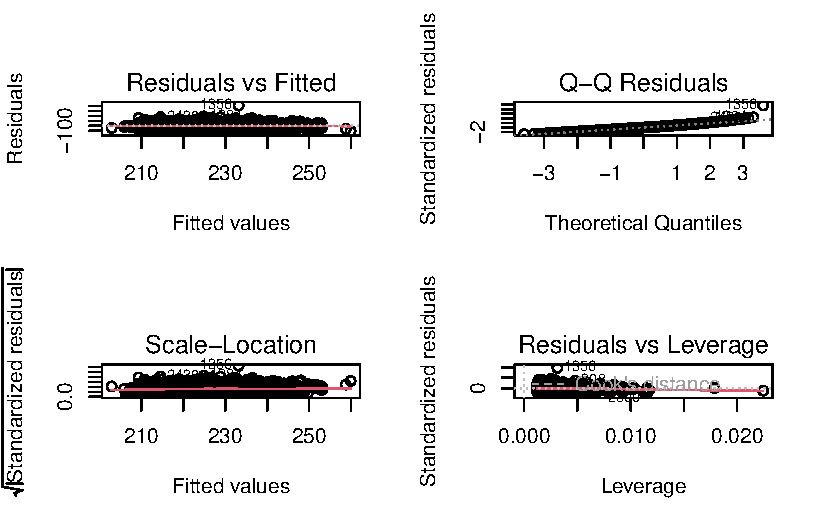
\includegraphics[width=0.85\linewidth,height=\textheight,keepaspectratio]{Section2/Numerical data analysis/06_linear_regression_files/figure-pdf/unnamed-chunk-9-1.pdf}
\end{center}

\begin{Shaded}
\begin{Highlighting}[]
\CommentTok{\# Perform model diagnostics and allow us to see if any of the assumptions failed to meet}
\NormalTok{performance}\SpecialCharTok{::}\FunctionTok{check\_model}\NormalTok{(model2)}
\end{Highlighting}
\end{Shaded}

\begin{itemize}
\tightlist
\item
  \textbf{Linearity:} plot observed \(y\) (or residuals) against fitted
  \(\hat y\). Points should scatter evenly around a horizontal line at
  zero with no curved pattern; a curved pattern suggests a nonlinear
  relationship is being forced into a straight line.
\item
  \textbf{Independence:} plot residuals in the order they were collected
  (or against time, if applicable). Random scatter with no runs or
  oscillating pattern supports independence; long runs of same-signed
  residuals suggest autocorrelation, common in time-series or
  repeated-measures data (see the Repeated Measures chapter for the
  proper fix).
\item
  \textbf{Normality:} a histogram of residuals should be roughly
  bell-shaped and centered near zero, and points on a Q-Q plot should
  fall close to the diagonal reference line.
\item
  \textbf{Equal variance (homoscedasticity):} plot residuals against
  fitted values; the spread should stay roughly constant across the
  range of fitted values. A ``funnel'' or ``fan'' shape --- residuals
  spreading out as fitted values increase --- indicates
  \textbf{heteroscedasticity}, which inflates or deflates standard
  errors and makes p-values unreliable.
\end{itemize}

\begin{tcolorbox}[enhanced jigsaw, bottomrule=.15mm, breakable, opacityback=0, toptitle=1mm, titlerule=0mm, bottomtitle=1mm, colback=white, arc=.35mm, rightrule=.15mm, toprule=.15mm, leftrule=.75mm, title=\textcolor{quarto-callout-note-color}{\faInfo}\hspace{0.5em}{Note}, colbacktitle=quarto-callout-note-color!10!white, colframe=quarto-callout-note-color-frame, coltitle=black, left=2mm, opacitybacktitle=0.6]

\textbf{How to report an assumption check (matches the standard 5-step
template used for hypothesis testing in this book):} ``\emph{Linearity}:
the fitted-vs-residual plot shows no curved pattern.
\emph{Independence}: residuals appear randomly scattered with no
discernible pattern. \emph{Normality}: the residual histogram is
unimodal and roughly symmetric, and the Q-Q plot points fall close to
the reference line. \emph{Equal variance}: residual spread looks
approximately constant across fitted values. In summary, all assumptions
appear reasonably satisfied.''

\end{tcolorbox}

\subsection{AIC, BIC, and RMSE}\label{aic-bic-and-rmse}

\begin{Shaded}
\begin{Highlighting}[]
\CommentTok{\# Determine the AIC, BIC, RMSE of the model}
\NormalTok{performance}\SpecialCharTok{::}\FunctionTok{model\_performance}\NormalTok{(model2)}
\end{Highlighting}
\end{Shaded}

\begin{verbatim}
#> # Indices of model performance
#> 
#> AIC     |    AICc |     BIC |    R2 | R2 (adj.) |   RMSE |  Sigma
#> -----------------------------------------------------------------
#> 32524.4 | 32524.5 | 32578.9 | 0.033 |     0.031 | 42.689 | 42.744
\end{verbatim}

AIC and BIC are \textbf{model-comparison} statistics --- lower values
indicate a better-fitting model relative to its complexity --- and are
most useful when comparing two or more candidate models (see the Model
Building and Selection chapter), rather than interpreted in isolation
for a single model. RMSE (root mean squared error) summarizes the
typical size of prediction error in the original units of \(y\).

\section{Worked Example: A Complete Analysis (Categorical + Continuous
Predictors)}\label{worked-example-a-complete-analysis-categorical-continuous-predictors}

Consider a classic textbook example: modeling baby birth weight (grams)
as a function of gestation length (\texttt{weeks}, continuous) and
maternal smoking status (\texttt{smoke}, categorical:
smoker/non-smoker), for \(n=100\) births. The fitted model is:

\[ \widehat{\text{BirthWeight}} = -2018.8 + 130.05\,\text{weeks} + 294.4\,\text{smoke(non-smoker vs. smoker)} \]

\textbf{Testing gestation length:} \(H_0:\beta_{weeks}=0\)
vs.~\(H_1:\beta_{weeks}\ne0\); \(t=8.96\), \(p<0.0001\) --- reject
\(H_0\); gestation length is significantly associated with birth weight.

\textbf{Testing smoking status:} \(H_0:\beta_{smoke}=0\)
vs.~\(H_1:\beta_{smoke}\ne0\); \(t=2.17\), \(p=0.0326\) --- reject
\(H_0\); smoking status is significantly associated with birth weight
after adjusting for gestation length.

\textbf{Interpretation:} for every additional week of gestation, average
birth weight increases by 130.05 g, holding smoking status constant; and
average birth weight for non-smoking mothers is 294.4 g higher than for
smoking mothers, holding gestation length constant.

We reproduce the same style of analysis on the \texttt{wcgs} data,
modeling cholesterol from age category and smoking status:

\begin{Shaded}
\begin{Highlighting}[]
\NormalTok{model3 }\OtherTok{\textless{}{-}} \FunctionTok{lm}\NormalTok{(chol }\SpecialCharTok{\textasciitilde{}}\NormalTok{ agec }\SpecialCharTok{+}\NormalTok{ smoke, }\AttributeTok{data =}\NormalTok{ data)}
\FunctionTok{summary}\NormalTok{(model3)}
\end{Highlighting}
\end{Shaded}

\begin{verbatim}
#> 
#> Call:
#> lm(formula = chol ~ agec + smoke, data = data)
#> 
#> Residuals:
#>     Min      1Q  Median      3Q     Max 
#> -133.90  -28.77   -3.09   26.22  424.23 
#> 
#> Coefficients:
#>             Estimate Std. Error t value Pr(>|t|)    
#> (Intercept)  216.115      1.983 108.991  < 2e-16 ***
#> agec41-45      4.655      2.267   2.054 0.040083 *  
#> agec46-50      6.956      2.431   2.861 0.004245 ** 
#> agec51-55     12.319      2.638   4.670 3.14e-06 ***
#> agec56-60     12.428      3.340   3.721 0.000202 ***
#> smokeYes       8.359      1.539   5.433 5.97e-08 ***
#> ---
#> Signif. codes:  0 '***' 0.001 '**' 0.01 '*' 0.05 '.' 0.1 ' ' 1
#> 
#> Residual standard error: 43.05 on 3136 degrees of freedom
#>   (12 observations deleted due to missingness)
#> Multiple R-squared:  0.01841,    Adjusted R-squared:  0.01685 
#> F-statistic: 11.76 on 5 and 3136 DF,  p-value: 2.718e-11
\end{verbatim}

\begin{Shaded}
\begin{Highlighting}[]
\NormalTok{sjPlot}\SpecialCharTok{::}\FunctionTok{tab\_model}\NormalTok{(model3)}
\end{Highlighting}
\end{Shaded}

\begin{longtable}[]{@{}cccc@{}}
\toprule\noalign{}
\endhead
\bottomrule\noalign{}
\endlastfoot
~ & \multicolumn{3}{c@{}}{%
chol} \\
Predictors & Estimates & CI & p \\
(Intercept) & 216.11 & 212.23~--~220.00 & \textbf{\textless0.001} \\
agec41-45 & 4.66 & 0.21~--~9.10 & \textbf{0.040} \\
agec46-50 & 6.96 & 2.19~--~11.72 & \textbf{0.004} \\
agec51-55 & 12.32 & 7.15~--~17.49 & \textbf{\textless0.001} \\
agec56-60 & 12.43 & 5.88~--~18.98 & \textbf{\textless0.001} \\
smoke {[}Yes{]} & 8.36 & 5.34~--~11.38 & \textbf{\textless0.001} \\
Observations & \multicolumn{3}{l@{}}{%
3142} \\
R\textsuperscript{2} / R\textsuperscript{2} adjusted &
\multicolumn{3}{l@{}}{%
0.018 / 0.017} \\
\end{longtable}

\begin{Shaded}
\begin{Highlighting}[]
\NormalTok{performance}\SpecialCharTok{::}\FunctionTok{check\_model}\NormalTok{(model3)}
\end{Highlighting}
\end{Shaded}

Chapter 6 introduced multiple linear regression and showed that a
coefficient's interpretation always comes with the phrase ``holding the
other predictors constant.'' This chapter asks two follow-up questions
that determine which predictors belong in a model, and how to interpret
them correctly once they're there: does the effect of my primary
predictor \textbf{change} across levels of another variable
(\textbf{interaction} / effect modification), and does another variable
\textbf{distort} the crude relationship between my primary predictor and
the outcome (\textbf{confounding})? These are two distinct phenomena,
checked with two distinct procedures, and confusing one for the other is
one of the most common errors in applied regression analysis.

\section{Interaction}\label{interaction}

An \textbf{interaction} (also called \textbf{effect modification}) is
present when the relationship between \(y\) and a predictor \(x_1\)
changes across the different values or levels of a second predictor
\(x_2\). We say \(x_2\) \textbf{moderates} the relationship between
\(y\) and \(x_1\) --- \(x_2\) is called an \textbf{effect modifier}.
Interaction is tested by adding a product term to the model:

\[ y = \beta_0 + \beta_1 x_1 + \beta_2 x_2 + \beta_3\,(x_1 \times x_2) + \varepsilon \]

Here \(x_1\) and \(x_2\) are the \textbf{main effects} and
\(x_1\times x_2\) is the \textbf{interaction term}; \(x_1\) and \(x_2\)
can each be continuous or categorical, in any combination
(continuous--continuous, continuous--categorical,
categorical--categorical).

\subsection{Hypothesis Test for
Interaction}\label{hypothesis-test-for-interaction}

\[ H_0: \beta_3 = 0 \qquad \text{vs.} \qquad H_1: \beta_3 \ne 0 \]

\begin{itemize}
\tightlist
\item
  If we \textbf{fail to reject} \(H_0\): interaction is not
  statistically significant. Remove the interaction term and re-fit the
  model with only the main effects.
\item
  If we \textbf{reject} \(H_0\): the relationship between \(x_1\) and
  \(y\) genuinely differs across values/levels of \(x_2\). The
  interaction term must be \textbf{kept}, and \(\beta_1\) can no longer
  be interpreted on its own --- the model must be interpreted by
  ``unfolding'' the interaction (below).
\end{itemize}

\begin{tcolorbox}[enhanced jigsaw, bottomrule=.15mm, breakable, opacityback=0, toptitle=1mm, titlerule=0mm, bottomtitle=1mm, colback=white, arc=.35mm, rightrule=.15mm, toprule=.15mm, leftrule=.75mm, title=\textcolor{quarto-callout-important-color}{\faExclamation}\hspace{0.5em}{Important}, colbacktitle=quarto-callout-important-color!10!white, colframe=quarto-callout-important-color-frame, coltitle=black, left=2mm, opacitybacktitle=0.6]

\textbf{Interaction is hierarchical.} If \(\beta_3\) (the interaction)
is significant, \emph{both} main effects \(x_1\) and \(x_2\) must remain
in the model regardless of whether their own individual p-values are
significant. It is not valid to drop a main effect while keeping the
interaction term that involves it.

\end{tcolorbox}

\subsection{Unfolding the Interaction
Term}\label{unfolding-the-interaction-term}

``Unfolding'' means holding the effect-modifying variable at a specific
value and simplifying the model algebraically to see the resulting slope
or group difference at that value.

\textbf{Two continuous predictors.} Plug a specific value of \(x_2\)
(e.g., \(x_2=10\)) into the model:

\[ \hat y = \hat\beta_0 + \hat\beta_1 x_1 + \hat\beta_2(10) + \hat\beta_3\,x_1(10) = \big[\hat\beta_0+10\hat\beta_2\big] + \big[\hat\beta_1+10\hat\beta_3\big]x_1 \]

The slope of \(x_1\) when \(x_2=10\) is \(\hat\beta_1+10\hat\beta_3\).
Repeating this at a few representative values of \(x_2\) (e.g., its
25th, 50th, and 75th percentiles) shows how the \(x_1\)--\(y\)
relationship shifts across the range of \(x_2\).

\textbf{One continuous, one categorical predictor.} If \(x_1\) is
continuous and \(x_2\) is a 0/1 categorical variable, plugging in
\(x_2=1\) gives the slope of \(x_1\) in that group
(\(\hat\beta_1+\hat\beta_3\)), and \(x_2=0\) gives the slope in the
reference group (\(\hat\beta_1\)). Alternatively, holding the continuous
variable fixed (e.g., age = 20) and simplifying shows the between-group
difference at that specific age.

\textbf{Two categorical predictors.} Holding each categorical variable
at a specific level in turn shows the group difference on the
\emph{other} variable, specific to that level (e.g., ``the male--female
difference in effectiveness for treatment method A'' vs.~``\ldots for
method B'').

\subsection{Worked Example: Interaction Between Two Continuous
Predictors}\label{worked-example-interaction-between-two-continuous-predictors}

Using the \texttt{wcgs} data, we test whether the relationship between
cholesterol and age depends on BMI:

\begin{Shaded}
\begin{Highlighting}[]
\NormalTok{model\_int1 }\OtherTok{\textless{}{-}} \FunctionTok{lm}\NormalTok{(chol }\SpecialCharTok{\textasciitilde{}}\NormalTok{ age }\SpecialCharTok{*}\NormalTok{ bmi, }\AttributeTok{data =}\NormalTok{ data)}
\FunctionTok{summary}\NormalTok{(model\_int1)}
\end{Highlighting}
\end{Shaded}

\begin{verbatim}
#> 
#> Call:
#> lm(formula = chol ~ age * bmi, data = data)
#> 
#> Residuals:
#>     Min      1Q  Median      3Q     Max 
#> -128.89  -28.28   -2.90   25.70  413.14 
#> 
#> Coefficients:
#>             Estimate Std. Error t value Pr(>|t|)  
#> (Intercept) 93.20940   61.83744   1.507   0.1318  
#> age          2.26130    1.32476   1.707   0.0879 .
#> bmi          4.13526    2.51092   1.647   0.0997 .
#> age:bmi     -0.06420    0.05376  -1.194   0.2325  
#> ---
#> Signif. codes:  0 '***' 0.001 '**' 0.01 '*' 0.05 '.' 0.1 ' ' 1
#> 
#> Residual standard error: 43.16 on 3138 degrees of freedom
#>   (12 observations deleted due to missingness)
#> Multiple R-squared:  0.01308,    Adjusted R-squared:  0.01213 
#> F-statistic: 13.86 on 3 and 3138 DF,  p-value: 5.619e-09
\end{verbatim}

If \texttt{age:bmi} is significant, the slope of cholesterol on age
differs across BMI values. We unfold by evaluating the age-slope at
representative BMI values (25th, 50th, 75th percentiles):

\begin{Shaded}
\begin{Highlighting}[]
\NormalTok{bmi\_q }\OtherTok{\textless{}{-}} \FunctionTok{quantile}\NormalTok{(data}\SpecialCharTok{$}\NormalTok{bmi, }\AttributeTok{probs =} \FunctionTok{c}\NormalTok{(}\FloatTok{0.25}\NormalTok{, }\FloatTok{0.5}\NormalTok{, }\FloatTok{0.75}\NormalTok{), }\AttributeTok{na.rm =} \ConstantTok{TRUE}\NormalTok{)}
\NormalTok{b }\OtherTok{\textless{}{-}} \FunctionTok{coef}\NormalTok{(model\_int1)}

\CommentTok{\# slope of age at each BMI quantile: beta\_age + beta\_(age:bmi) * bmi}
\NormalTok{slopes }\OtherTok{\textless{}{-}}\NormalTok{ b[}\StringTok{"age"}\NormalTok{] }\SpecialCharTok{+}\NormalTok{ b[}\StringTok{"age:bmi"}\NormalTok{] }\SpecialCharTok{*}\NormalTok{ bmi\_q}
\FunctionTok{data.frame}\NormalTok{(}\AttributeTok{bmi =}\NormalTok{ bmi\_q, }\AttributeTok{slope\_of\_age =}\NormalTok{ slopes)}
\end{Highlighting}
\end{Shaded}

\begin{verbatim}
#>          bmi slope_of_age
#> 25% 22.95510    0.7875816
#> 50% 24.38980    0.6954741
#> 75% 25.84016    0.6023603
\end{verbatim}

\subsection{Worked Example: Interaction Between a Continuous and a
Categorical
Predictor}\label{worked-example-interaction-between-a-continuous-and-a-categorical-predictor}

\begin{Shaded}
\begin{Highlighting}[]
\NormalTok{model\_int2 }\OtherTok{\textless{}{-}} \FunctionTok{lm}\NormalTok{(chol }\SpecialCharTok{\textasciitilde{}}\NormalTok{ sbp }\SpecialCharTok{*}\NormalTok{ dibpat, }\AttributeTok{data =}\NormalTok{ data)}
\FunctionTok{summary}\NormalTok{(model\_int2)}
\end{Highlighting}
\end{Shaded}

\begin{verbatim}
#> 
#> Call:
#> lm(formula = chol ~ sbp * dibpat, data = data)
#> 
#> Residuals:
#>     Min      1Q  Median      3Q     Max 
#> -124.99  -29.00   -3.25   26.60  408.01 
#> 
#> Coefficients:
#>                   Estimate Std. Error t value Pr(>|t|)    
#> (Intercept)      185.10952    9.02373  20.514  < 2e-16 ***
#> sbp                0.33688    0.06903   4.880 1.11e-06 ***
#> dibpatType B      -6.24784   13.31228  -0.469    0.639    
#> sbp:dibpatType B   0.01639    0.10292   0.159    0.874    
#> ---
#> Signif. codes:  0 '***' 0.001 '**' 0.01 '*' 0.05 '.' 0.1 ' ' 1
#> 
#> Residual standard error: 43.06 on 3138 degrees of freedom
#>   (12 observations deleted due to missingness)
#> Multiple R-squared:  0.01741,    Adjusted R-squared:  0.01647 
#> F-statistic: 18.54 on 3 and 3138 DF,  p-value: 6.423e-12
\end{verbatim}

\begin{Shaded}
\begin{Highlighting}[]
\CommentTok{\# If interaction is significant, examine the slope of sbp within each dibpat group directly}
\NormalTok{data }\SpecialCharTok{|\textgreater{}}
  \FunctionTok{group\_by}\NormalTok{(dibpat) }\SpecialCharTok{|\textgreater{}}
  \FunctionTok{summarise}\NormalTok{(}\AttributeTok{slope =} \FunctionTok{coef}\NormalTok{(}\FunctionTok{lm}\NormalTok{(chol }\SpecialCharTok{\textasciitilde{}}\NormalTok{ sbp))[}\DecValTok{2}\NormalTok{], }\AttributeTok{.groups =} \StringTok{"drop"}\NormalTok{)}
\end{Highlighting}
\end{Shaded}

\begin{verbatim}
#> # A tibble: 2 x 2
#>   dibpat slope
#>   <chr>  <dbl>
#> 1 Type A 0.337
#> 2 Type B 0.353
\end{verbatim}

\begin{tcolorbox}[enhanced jigsaw, bottomrule=.15mm, breakable, opacityback=0, toptitle=1mm, titlerule=0mm, bottomtitle=1mm, colback=white, arc=.35mm, rightrule=.15mm, toprule=.15mm, leftrule=.75mm, title=\textcolor{quarto-callout-tip-color}{\faLightbulb}\hspace{0.5em}{Tip}, colbacktitle=quarto-callout-tip-color!10!white, colframe=quarto-callout-tip-color-frame, coltitle=black, left=2mm, opacitybacktitle=0.6]

R and most modeling packages can ``unfold'' an interaction automatically
using estimated marginal means --- the \texttt{emmeans} package's
\texttt{emtrends()} (for continuous-by-group slopes) and
\texttt{emmeans()} (for group comparisons at fixed covariate values)
save you from doing the by-hand algebra shown above.

\end{tcolorbox}

\section{Confounding}\label{confounding}

Even when interaction is absent, a third variable can still distort the
crude (unadjusted) relationship between a primary predictor \(x\) and
outcome \(y\) if it is associated with \textbf{both}. Such a variable is
called a \textbf{confounder}.

A variable \(z\) is a confounder of the \(x\)--\(y\) relationship if:
(1) \(z\) is associated with the outcome \(y\); (2) \(z\) is associated
with the predictor \(x\); and (3) \(z\) is \textbf{not} an intermediate
step on the causal pathway from \(x\) to \(y\) (i.e., not a mediator).
Classic example: studying the relationship between physical exercise
(\(x\)) and blood pressure (\(y\)), age (\(z\)) is a likely confounder
--- older individuals tend to exercise less \emph{and} have higher blood
pressure, so a naive analysis could show a spurious association between
exercise and blood pressure that is really just an age effect.

\subsection{Detecting Confounding: The 10\%
Rule}\label{detecting-confounding-the-10-rule}

Compare the coefficient for \(x\) in the \textbf{crude} (unadjusted)
model to the coefficient for \(x\) in the \textbf{adjusted} model (with
\(z\) added):

\[ \text{Crude: } \hat y = \hat\beta_0 + \hat\beta_1 x \qquad \qquad \text{Adjusted: } \hat y = \hat\beta_0 + \hat\beta_1 x + \hat\beta_2 z \]

\[ \%\ \text{change} = \frac{\hat\beta_{1,\,adjusted} - \hat\beta_{1,\,crude}}{\hat\beta_{1,\,adjusted}} \times 100\% \]

\begin{tcolorbox}[enhanced jigsaw, bottomrule=.15mm, breakable, opacityback=0, toptitle=1mm, titlerule=0mm, bottomtitle=1mm, colback=white, arc=.35mm, rightrule=.15mm, toprule=.15mm, leftrule=.75mm, title=\textcolor{quarto-callout-note-color}{\faInfo}\hspace{0.5em}{Note}, colbacktitle=quarto-callout-note-color!10!white, colframe=quarto-callout-note-color-frame, coltitle=black, left=2mm, opacitybacktitle=0.6]

Two versions of this formula circulate --- an ``epidemiological''
version (dividing by the \textbf{adjusted} coefficient, shown above) and
a ``statistical'' version (dividing by the \textbf{crude} coefficient).
They can give different percentages when the crude and adjusted
estimates differ substantially. This book follows the epidemiological
convention (divide by the adjusted coefficient), consistent with
standard epidemiology practice.

\end{tcolorbox}

If the crude and adjusted coefficients for \(x\) differ by \textbf{more
than 10\%}, \(z\) is considered a confounder and should be retained in
the model, \emph{regardless of whether} \(z\)'s own coefficient is
statistically significant --- confounding is a property of how much
\(z\) changes the \(x\) estimate, not whether \(z\) itself is
``significant.''

\subsection{Worked Example: Testing for
Confounding}\label{worked-example-testing-for-confounding}

Does behavior pattern (\texttt{dibpat}) confound the relationship
between smoking and cholesterol?

\begin{Shaded}
\begin{Highlighting}[]
\CommentTok{\# Crude model}
\NormalTok{crude }\OtherTok{\textless{}{-}} \FunctionTok{lm}\NormalTok{(chol }\SpecialCharTok{\textasciitilde{}}\NormalTok{ smoke, }\AttributeTok{data =}\NormalTok{ data)}
\FunctionTok{coef}\NormalTok{(crude)[}\StringTok{"smoke1"}\NormalTok{]}
\end{Highlighting}
\end{Shaded}

\begin{verbatim}
#> <NA> 
#>   NA
\end{verbatim}

\begin{Shaded}
\begin{Highlighting}[]
\CommentTok{\# Adjusted model}
\NormalTok{adjusted }\OtherTok{\textless{}{-}} \FunctionTok{lm}\NormalTok{(chol }\SpecialCharTok{\textasciitilde{}}\NormalTok{ smoke }\SpecialCharTok{+}\NormalTok{ dibpat, }\AttributeTok{data =}\NormalTok{ data)}
\FunctionTok{coef}\NormalTok{(adjusted)[}\StringTok{"smoke1"}\NormalTok{]}
\end{Highlighting}
\end{Shaded}

\begin{verbatim}
#> <NA> 
#>   NA
\end{verbatim}

\begin{Shaded}
\begin{Highlighting}[]
\NormalTok{pct\_change }\OtherTok{\textless{}{-}}\NormalTok{ (}\FunctionTok{coef}\NormalTok{(adjusted)[}\StringTok{"smoke1"}\NormalTok{] }\SpecialCharTok{{-}} \FunctionTok{coef}\NormalTok{(crude)[}\StringTok{"smoke1"}\NormalTok{]) }\SpecialCharTok{/} \FunctionTok{coef}\NormalTok{(adjusted)[}\StringTok{"smoke1"}\NormalTok{] }\SpecialCharTok{*} \DecValTok{100}
\NormalTok{pct\_change}
\end{Highlighting}
\end{Shaded}

\begin{verbatim}
#> <NA> 
#>   NA
\end{verbatim}

\textbf{Interpretation:} if \texttt{pct\_change} exceeds 10\% in
magnitude, \texttt{dibpat} is a confounder of the smoking--cholesterol
relationship and should remain in the model even if its own p-value is
not significant; if it is under 10\%, \texttt{dibpat} is not an
important confounder here and can be dropped for parsimony (assuming it
also shows no significant interaction with smoking).

\section{Interaction and Confounding Can
Co-Occur}\label{interaction-and-confounding-can-co-occur}

A variable can simultaneously be an effect modifier \emph{and} a
confounder. The recommended order of operations, used throughout this
book and consistent with standard model-building practice (see the Model
Building and Selection chapter):

\begin{enumerate}
\def\labelenumi{\arabic{enumi}.}
\tightlist
\item
  \textbf{Test for interaction first.} Fit the model with the product
  term and test \(H_0:\beta_3=0\).
\item
  \textbf{If interaction is significant}, keep it (with both main
  effects) and interpret the model by unfolding --- do \textbf{not}
  proceed to a confounding check, since a single ``adjusted''
  coefficient is no longer meaningful when the effect genuinely varies
  across the modifier's levels.
\item
  \textbf{If interaction is not significant}, drop the interaction term,
  re-fit the main-effects-only model, and \textbf{then} test the same
  variable for confounding using the 10\% rule.
\end{enumerate}

\begin{tcolorbox}[enhanced jigsaw, bottomrule=.15mm, breakable, opacityback=0, toptitle=1mm, titlerule=0mm, bottomtitle=1mm, colback=white, arc=.35mm, rightrule=.15mm, toprule=.15mm, leftrule=.75mm, title=\textcolor{quarto-callout-tip-color}{\faLightbulb}\hspace{0.5em}{Tip}, colbacktitle=quarto-callout-tip-color!10!white, colframe=quarto-callout-tip-color-frame, coltitle=black, left=2mm, opacitybacktitle=0.6]

Epidemiologists often use the term ``effect modification'' for what
statisticians call interaction, and reserve ``confounding'' strictly for
the distortion of a crude estimate by a third variable that is
\emph{not} a mediator. Keeping this distinction in mind avoids
``adjusting away'' a genuine, biologically meaningful
effect-modification finding, and avoids reporting a single misleading
adjusted estimate when the true relationship is not uniform across
subgroups.

\end{tcolorbox}

Every regression model requires a decision about which predictors to
include. That decision should be driven by the goal of the analysis,
which falls into one of two categories, and the two categories call for
genuinely different strategies.

\section{Two Goals of Regression
Modeling}\label{two-goals-of-regression-modeling}

\begin{itemize}
\tightlist
\item
  \textbf{Aim 1 --- Association.} The research question centers on a
  single exposure of primary interest (e.g., how does smoking, together
  with age and other factors, relate to lung cancer risk?). The other
  variables are included only to the extent that they meaningfully
  influence the exposure--outcome relationship (as confounders or effect
  modifiers) --- not for their own sake.
\item
  \textbf{Aim 2 --- Prediction.} The research question is about building
  the best possible predictive model for the outcome, without a single
  variable of primary interest (e.g., predicting whether a loan
  applicant will default, using whatever combination of variables
  improves accuracy). Here it is reasonable to consider many candidate
  predictors and let a selection procedure decide which combination
  performs best.
\end{itemize}

\begin{tcolorbox}[enhanced jigsaw, bottomrule=.15mm, breakable, opacityback=0, toptitle=1mm, titlerule=0mm, bottomtitle=1mm, colback=white, arc=.35mm, rightrule=.15mm, toprule=.15mm, leftrule=.75mm, title=\textcolor{quarto-callout-important-color}{\faExclamation}\hspace{0.5em}{Important}, colbacktitle=quarto-callout-important-color!10!white, colframe=quarto-callout-important-color-frame, coltitle=black, left=2mm, opacitybacktitle=0.6]

These two aims call for different procedures. \textbf{Automated
stepwise-style selection techniques should not be used for Aim 1
(association) studies} --- for a study with a primary exposure of
interest, the model is built by explicitly checking each candidate
covariate for interaction and confounding with the exposure, described
next, not by an automated algorithm that could drop or retain the
exposure itself based on statistical significance.

\end{tcolorbox}

\section{Aim 1: Building an Association
Model}\label{aim-1-building-an-association-model}

When the goal is a valid, interpretable estimate of one primary
exposure's effect, follow this sequence:

\begin{enumerate}
\def\labelenumi{\arabic{enumi}.}
\tightlist
\item
  Fit the \textbf{crude model}: \(y = \beta_0+\beta_1 x + \varepsilon\),
  with \(x\) the primary exposure, to establish the baseline
  (unadjusted) relationship.
\item
  \textbf{Screen} all other variables the dataset has available that
  might plausibly influence the exposure--outcome relationship,
  biologically or through prior literature.
\item
  For each candidate variable \(z\), \textbf{check for interaction} with
  \(x\) (fit
  \(y=\beta_0+\beta_1x+\beta_2z+\beta_3(x{\times}z)+\varepsilon\) and
  test \(H_0:\beta_3=0\), per the Interaction and Confounding chapter).
\item
  For candidates whose interaction with \(x\) is \textbf{not}
  significant, \textbf{check for confounding} using the 10\% rule
  (compare \(\hat\beta_1\) crude vs.~adjusted for \(z\)).
\item
  Build the \textbf{final model} including \(x\), all significant
  interaction terms (with their required main effects), and all
  identified confounders. There is no algorithmic ``model selection''
  step in an association study --- every included/excluded variable is
  justified individually by interaction or confounding, not by an
  automated fit-improvement criterion.
\end{enumerate}

\begin{Shaded}
\begin{Highlighting}[]
\CommentTok{\# Aim 1 example: primary exposure = smoke, outcome = chol, candidate covariates = agec, bmi, dibpat}
\NormalTok{crude }\OtherTok{\textless{}{-}} \FunctionTok{lm}\NormalTok{(chol }\SpecialCharTok{\textasciitilde{}}\NormalTok{ smoke, }\AttributeTok{data =}\NormalTok{ data)}
\FunctionTok{coef}\NormalTok{(crude)[}\StringTok{"smokeYes"}\NormalTok{]}
\end{Highlighting}
\end{Shaded}

\begin{verbatim}
#> smokeYes 
#> 8.474704
\end{verbatim}

\begin{Shaded}
\begin{Highlighting}[]
\CommentTok{\# Step: check interaction between smoke and each candidate}
\FunctionTok{summary}\NormalTok{(}\FunctionTok{lm}\NormalTok{(chol }\SpecialCharTok{\textasciitilde{}}\NormalTok{ smoke }\SpecialCharTok{*}\NormalTok{ bmi, }\AttributeTok{data =}\NormalTok{ data))}\SpecialCharTok{$}\NormalTok{coefficients[}\StringTok{"smokeYes:bmi"}\NormalTok{, ]}
\end{Highlighting}
\end{Shaded}

\begin{verbatim}
#>   Estimate Std. Error    t value   Pr(>|t|) 
#>  0.4100055  0.6059834  0.6765953  0.4987127
\end{verbatim}

\begin{Shaded}
\begin{Highlighting}[]
\CommentTok{\# Step: for candidates without significant interaction, check confounding (10\% rule)}
\NormalTok{adj\_bmi }\OtherTok{\textless{}{-}} \FunctionTok{lm}\NormalTok{(chol }\SpecialCharTok{\textasciitilde{}}\NormalTok{ smoke }\SpecialCharTok{+}\NormalTok{ bmi, }\AttributeTok{data =}\NormalTok{ data)}
\NormalTok{(}\FunctionTok{coef}\NormalTok{(adj\_bmi)[}\StringTok{"smokeYes"}\NormalTok{] }\SpecialCharTok{{-}} \FunctionTok{coef}\NormalTok{(crude)[}\StringTok{"smokeYes"}\NormalTok{]) }\SpecialCharTok{/} \FunctionTok{coef}\NormalTok{(adj\_bmi)[}\StringTok{"smokeYes"}\NormalTok{] }\SpecialCharTok{*} \DecValTok{100}
\end{Highlighting}
\end{Shaded}

\begin{verbatim}
#> smokeYes 
#> 11.22982
\end{verbatim}

\section{Aim 2: Building a Prediction
Model}\label{aim-2-building-a-prediction-model}

When the goal is pure prediction, it is reasonable to include as many
candidate predictors as are available, then use a selection procedure to
find the subset that best balances fit against complexity.

\subsection{Step 1: Initial Screening}\label{step-1-initial-screening}

Fit a separate simple regression of \(y\) on each candidate predictor,
and retain any predictor with p \textless{} 0.5 (a deliberately
\textbf{generous} threshold for this first pass, wider than the usual
0.05, so that predictors with only weak individual associations are not
prematurely excluded before the multivariable selection step gets a
chance to evaluate them jointly).

\begin{Shaded}
\begin{Highlighting}[]
\NormalTok{candidates }\OtherTok{\textless{}{-}} \FunctionTok{c}\NormalTok{(}\StringTok{"sbp"}\NormalTok{, }\StringTok{"agec"}\NormalTok{, }\StringTok{"bmi"}\NormalTok{, }\StringTok{"smoke"}\NormalTok{, }\StringTok{"dibpat"}\NormalTok{, }\StringTok{"ncigs"}\NormalTok{)}
\NormalTok{screen }\OtherTok{\textless{}{-}}\NormalTok{ purrr}\SpecialCharTok{::}\FunctionTok{map\_dfr}\NormalTok{(candidates, }\ControlFlowTok{function}\NormalTok{(v) \{}
\NormalTok{  f }\OtherTok{\textless{}{-}} \FunctionTok{as.formula}\NormalTok{(}\FunctionTok{paste}\NormalTok{(}\StringTok{"chol \textasciitilde{}"}\NormalTok{, v))}
\NormalTok{  m }\OtherTok{\textless{}{-}} \FunctionTok{lm}\NormalTok{(f, }\AttributeTok{data =}\NormalTok{ data)}
\NormalTok{  broom}\SpecialCharTok{::}\FunctionTok{tidy}\NormalTok{(}\FunctionTok{anova}\NormalTok{(m))[}\DecValTok{1}\NormalTok{, ] }\SpecialCharTok{|\textgreater{}}\NormalTok{ dplyr}\SpecialCharTok{::}\FunctionTok{mutate}\NormalTok{(}\AttributeTok{variable =}\NormalTok{ v)}
\NormalTok{\})}
\NormalTok{screen }\SpecialCharTok{|\textgreater{}}\NormalTok{ dplyr}\SpecialCharTok{::}\FunctionTok{select}\NormalTok{(variable, p.value)}
\end{Highlighting}
\end{Shaded}

\begin{verbatim}
#> # A tibble: 6 x 2
#>   variable  p.value
#>   <chr>       <dbl>
#> 1 sbp      4.47e-12
#> 2 agec     8.12e- 6
#> 3 bmi      7.44e- 5
#> 4 smoke    4.36e- 8
#> 5 dibpat   1.39e- 3
#> 6 ncigs    6.92e- 8
\end{verbatim}

\subsection{Step 2: Model Selection
Techniques}\label{step-2-model-selection-techniques}

Three classic iterative procedures search the space of predictor
subsets:

\begin{itemize}
\tightlist
\item
  \textbf{Forward selection:} start with no predictors; at each step,
  add the one variable that most improves the model (e.g., largest
  increase in adjusted \(R^2\), or smallest p-value); stop when no
  remaining variable improves the model further.
\item
  \textbf{Backward selection:} start with \textbf{all} candidate
  predictors; at each step, remove the least useful variable (smallest
  adjusted \(R^2\) drop, or largest p-value above a cutoff, e.g., 0.10);
  stop when every remaining variable clears the cutoff.
\item
  \textbf{Stepwise selection:} a combination of the two --- after each
  addition, previously added variables are re-examined for possible
  removal, and vice versa.
\end{itemize}

\begin{Shaded}
\begin{Highlighting}[]
\CommentTok{\# R implementation using AIC{-}based stepwise selection (step()), the R analogue of PROC GLMSELECT}
\NormalTok{full\_model }\OtherTok{\textless{}{-}} \FunctionTok{lm}\NormalTok{(chol }\SpecialCharTok{\textasciitilde{}}\NormalTok{ sbp }\SpecialCharTok{+}\NormalTok{ agec }\SpecialCharTok{+}\NormalTok{ bmi }\SpecialCharTok{+}\NormalTok{ smoke }\SpecialCharTok{+}\NormalTok{ dibpat }\SpecialCharTok{+}\NormalTok{ ncigs, }\AttributeTok{data =}\NormalTok{ data)}
\NormalTok{null\_model }\OtherTok{\textless{}{-}} \FunctionTok{lm}\NormalTok{(chol }\SpecialCharTok{\textasciitilde{}} \DecValTok{1}\NormalTok{, }\AttributeTok{data =}\NormalTok{ data)}

\CommentTok{\# Forward}
\NormalTok{step\_fwd }\OtherTok{\textless{}{-}} \FunctionTok{step}\NormalTok{(null\_model, }\AttributeTok{scope =} \FunctionTok{list}\NormalTok{(}\AttributeTok{lower =}\NormalTok{ null\_model, }\AttributeTok{upper =}\NormalTok{ full\_model),}
                  \AttributeTok{direction =} \StringTok{"forward"}\NormalTok{, }\AttributeTok{trace =} \ConstantTok{FALSE}\NormalTok{)}
\FunctionTok{summary}\NormalTok{(step\_fwd)}
\end{Highlighting}
\end{Shaded}

\begin{verbatim}
#> 
#> Call:
#> lm(formula = chol ~ sbp + smoke + agec + bmi + dibpat, data = data)
#> 
#> Residuals:
#>     Min      1Q  Median      3Q     Max 
#> -130.57  -27.87   -2.85   26.04  410.23 
#> 
#> Coefficients:
#>               Estimate Std. Error t value Pr(>|t|)    
#> (Intercept)  161.30071    8.99516  17.932  < 2e-16 ***
#> sbp            0.26350    0.05381   4.897 1.02e-06 ***
#> smokeYes       8.85966    1.54717   5.726 1.12e-08 ***
#> agec41-45      4.21478    2.25161   1.872  0.06131 .  
#> agec46-50      5.49047    2.42316   2.266  0.02353 *  
#> agec51-55      9.96307    2.64659   3.764  0.00017 ***
#> agec56-60     10.03027    3.33843   3.004  0.00268 ** 
#> bmi            0.95171    0.31420   3.029  0.00247 ** 
#> dibpatType B  -3.15496    1.53796  -2.051  0.04031 *  
#> ---
#> Signif. codes:  0 '***' 0.001 '**' 0.01 '*' 0.05 '.' 0.1 ' ' 1
#> 
#> Residual standard error: 42.72 on 3133 degrees of freedom
#>   (12 observations deleted due to missingness)
#> Multiple R-squared:  0.03437,    Adjusted R-squared:  0.03191 
#> F-statistic: 13.94 on 8 and 3133 DF,  p-value: < 2.2e-16
\end{verbatim}

\begin{Shaded}
\begin{Highlighting}[]
\CommentTok{\# Backward}
\NormalTok{step\_back }\OtherTok{\textless{}{-}} \FunctionTok{step}\NormalTok{(full\_model, }\AttributeTok{direction =} \StringTok{"backward"}\NormalTok{, }\AttributeTok{trace =} \ConstantTok{FALSE}\NormalTok{)}
\FunctionTok{summary}\NormalTok{(step\_back)}
\end{Highlighting}
\end{Shaded}

\begin{verbatim}
#> 
#> Call:
#> lm(formula = chol ~ sbp + agec + bmi + smoke + dibpat, data = data)
#> 
#> Residuals:
#>     Min      1Q  Median      3Q     Max 
#> -130.57  -27.87   -2.85   26.04  410.23 
#> 
#> Coefficients:
#>               Estimate Std. Error t value Pr(>|t|)    
#> (Intercept)  161.30071    8.99516  17.932  < 2e-16 ***
#> sbp            0.26350    0.05381   4.897 1.02e-06 ***
#> agec41-45      4.21478    2.25161   1.872  0.06131 .  
#> agec46-50      5.49047    2.42316   2.266  0.02353 *  
#> agec51-55      9.96307    2.64659   3.764  0.00017 ***
#> agec56-60     10.03027    3.33843   3.004  0.00268 ** 
#> bmi            0.95171    0.31420   3.029  0.00247 ** 
#> smokeYes       8.85966    1.54717   5.726 1.12e-08 ***
#> dibpatType B  -3.15496    1.53796  -2.051  0.04031 *  
#> ---
#> Signif. codes:  0 '***' 0.001 '**' 0.01 '*' 0.05 '.' 0.1 ' ' 1
#> 
#> Residual standard error: 42.72 on 3133 degrees of freedom
#>   (12 observations deleted due to missingness)
#> Multiple R-squared:  0.03437,    Adjusted R-squared:  0.03191 
#> F-statistic: 13.94 on 8 and 3133 DF,  p-value: < 2.2e-16
\end{verbatim}

\begin{Shaded}
\begin{Highlighting}[]
\CommentTok{\# Stepwise (both directions)}
\NormalTok{step\_both }\OtherTok{\textless{}{-}} \FunctionTok{step}\NormalTok{(full\_model, }\AttributeTok{direction =} \StringTok{"both"}\NormalTok{, }\AttributeTok{trace =} \ConstantTok{FALSE}\NormalTok{)}
\FunctionTok{summary}\NormalTok{(step\_both)}
\end{Highlighting}
\end{Shaded}

\begin{verbatim}
#> 
#> Call:
#> lm(formula = chol ~ sbp + agec + bmi + smoke + dibpat, data = data)
#> 
#> Residuals:
#>     Min      1Q  Median      3Q     Max 
#> -130.57  -27.87   -2.85   26.04  410.23 
#> 
#> Coefficients:
#>               Estimate Std. Error t value Pr(>|t|)    
#> (Intercept)  161.30071    8.99516  17.932  < 2e-16 ***
#> sbp            0.26350    0.05381   4.897 1.02e-06 ***
#> agec41-45      4.21478    2.25161   1.872  0.06131 .  
#> agec46-50      5.49047    2.42316   2.266  0.02353 *  
#> agec51-55      9.96307    2.64659   3.764  0.00017 ***
#> agec56-60     10.03027    3.33843   3.004  0.00268 ** 
#> bmi            0.95171    0.31420   3.029  0.00247 ** 
#> smokeYes       8.85966    1.54717   5.726 1.12e-08 ***
#> dibpatType B  -3.15496    1.53796  -2.051  0.04031 *  
#> ---
#> Signif. codes:  0 '***' 0.001 '**' 0.01 '*' 0.05 '.' 0.1 ' ' 1
#> 
#> Residual standard error: 42.72 on 3133 degrees of freedom
#>   (12 observations deleted due to missingness)
#> Multiple R-squared:  0.03437,    Adjusted R-squared:  0.03191 
#> F-statistic: 13.94 on 8 and 3133 DF,  p-value: < 2.2e-16
\end{verbatim}

\begin{tcolorbox}[enhanced jigsaw, bottomrule=.15mm, breakable, opacityback=0, toptitle=1mm, titlerule=0mm, bottomtitle=1mm, colback=white, arc=.35mm, rightrule=.15mm, toprule=.15mm, leftrule=.75mm, title=\textcolor{quarto-callout-note-color}{\faInfo}\hspace{0.5em}{Note}, colbacktitle=quarto-callout-note-color!10!white, colframe=quarto-callout-note-color-frame, coltitle=black, left=2mm, opacitybacktitle=0.6]

\texttt{step()} in R uses \textbf{AIC} as its default selection
criterion rather than adjusted \(R^2\) or a fixed p-value cutoff, but
the underlying logic (add/remove one variable at a time, re-evaluate,
repeat until no improvement) is identical to the manual
forward/backward/stepwise procedures. Different criteria can
occasionally select different ``best'' models; in practice, forward,
backward, and stepwise selection tend to agree more often than not,
especially when predictors are not highly correlated with one another.

\end{tcolorbox}

\subsection{Selection Criteria}\label{selection-criteria}

\begin{longtable}[]{@{}
  >{\raggedright\arraybackslash}p{(\linewidth - 4\tabcolsep) * \real{0.3333}}
  >{\raggedright\arraybackslash}p{(\linewidth - 4\tabcolsep) * \real{0.3333}}
  >{\raggedright\arraybackslash}p{(\linewidth - 4\tabcolsep) * \real{0.3333}}@{}}
\toprule\noalign{}
\begin{minipage}[b]{\linewidth}\raggedright
Criterion
\end{minipage} & \begin{minipage}[b]{\linewidth}\raggedright
Interpretation
\end{minipage} & \begin{minipage}[b]{\linewidth}\raggedright
Rule of thumb
\end{minipage} \\
\midrule\noalign{}
\endhead
\bottomrule\noalign{}
\endlastfoot
Adjusted \(R^2\) & \(R^2\) penalized for the number of predictors \(p\):
\(R_a^2 = 1-\dfrac{MS_{Error}}{SS_{Total}/(n-p-1)}\) & Larger is
better \\
AIC / BIC & Likelihood-based fit penalized for model complexity &
Smaller is better \\
\(MS_{Error}\) & Estimate of \(\sigma^2\); large values indicate a
poorly fitting model & Smaller is better \\
\(C_p\) (Mallows') & Balances bias and variance; compare to \(p+1\) &
\(C_p\) close to (or below) \(p+1\) is good \\
PRESS & Sum of squared \textbf{leave-one-out} prediction errors --- a
direct check of predictive (not just fitted) performance & Smaller is
better \\
\end{longtable}

Ordinary \(R^2\) is a poor selection criterion on its own because it can
never decrease when a new predictor is added (even a useless one) --- it
will always favor the largest possible model. Adjusted \(R^2\), AIC, and
BIC all correct for this by penalizing model size.

\section{\texorpdfstring{Comparing Two Nested Models Directly: The Delta
(\(\Delta\))
Method}{Comparing Two Nested Models Directly: The Delta (\textbackslash Delta) Method}}\label{comparing-two-nested-models-directly-the-delta-delta-method}

Rather than relying on a general-purpose criterion, two specific
\textbf{nested} models (a ``full'' model and a ``reduced'' model that
drops a subset of the full model's predictors) can be compared directly
with a partial F-test:

\[ H_0: R^2_{full} - R^2_{reduced} = 0 \qquad \text{vs.} \qquad H_1: R^2_{full} - R^2_{reduced} > 0 \]

\[ F_0 = \frac{\left(SS_{Error,\,reduced} - SS_{Error,\,full}\right)/\left(df_{reduced}-df_{full}\right)}{MS_{Error,\,full}} \]

If we \textbf{fail to reject} \(H_0\), the extra predictors in the full
model do not explain significantly more variation than the reduced model
--- by the principle of \textbf{parsimony}, prefer the simpler (reduced)
model. If we \textbf{reject} \(H_0\), the additional predictors matter,
and the full model should be kept.

\begin{Shaded}
\begin{Highlighting}[]
\NormalTok{full  }\OtherTok{\textless{}{-}} \FunctionTok{lm}\NormalTok{(chol }\SpecialCharTok{\textasciitilde{}}\NormalTok{ sbp }\SpecialCharTok{+}\NormalTok{ agec }\SpecialCharTok{+}\NormalTok{ bmi }\SpecialCharTok{+}\NormalTok{ smoke, }\AttributeTok{data =}\NormalTok{ data)}
\NormalTok{reduced }\OtherTok{\textless{}{-}} \FunctionTok{lm}\NormalTok{(chol }\SpecialCharTok{\textasciitilde{}}\NormalTok{ sbp }\SpecialCharTok{+}\NormalTok{ agec, }\AttributeTok{data =}\NormalTok{ data)}

\FunctionTok{anova}\NormalTok{(reduced, full)   }\CommentTok{\# R\textquotesingle{}s anova() on two nested lm objects performs exactly this partial F{-}test}
\end{Highlighting}
\end{Shaded}

\begin{verbatim}
#> Analysis of Variance Table
#> 
#> Model 1: chol ~ sbp + agec
#> Model 2: chol ~ sbp + agec + bmi + smoke
#>   Res.Df     RSS Df Sum of Sq      F    Pr(>F)    
#> 1   3136 5797619                                  
#> 2   3134 5725957  2     71662 19.611 3.434e-09 ***
#> ---
#> Signif. codes:  0 '***' 0.001 '**' 0.01 '*' 0.05 '.' 0.1 ' ' 1
\end{verbatim}

\textbf{Interpretation:} the \texttt{anova(reduced,\ full)} output
reports \(F_0\), its degrees of freedom, and a p-value directly. A
p-value below 0.05 supports keeping the full model (the added predictors
--- \texttt{bmi} and \texttt{smoke} here, jointly improve the fit
significantly); a p-value above 0.05 supports the simpler, reduced
model.

\section{Model Assumption Violations:
Collinearity}\label{model-assumption-violations-collinearity}

\textbf{Collinearity} occurs when one predictor is (nearly) a linear
combination of one or more other predictors in the model; with two or
more such relationships, this is called \textbf{multicollinearity}.
Collinearity does not bias the coefficient estimates, but it inflates
their standard errors which makes coefficients unstable, sometimes
flipping sign or losing significance simply because the model cannot
distinguish the separate contributions of highly correlated predictors.

\subsection{Detecting Collinearity: The Variance Inflation Factor
(VIF)}\label{detecting-collinearity-the-variance-inflation-factor-vif}

For predictor \(x_j\), regress \(x_j\) on all the \emph{other}
predictors in the model, obtain that auxiliary regression's \(R_j^2\),
and compute:

\[ VIF_j = \frac{1}{1-R_j^2} \]

A large \(VIF_j\) means \(x_j\) is well explained by the other
predictors (i.e., largely redundant with them). A conservative cutoff is
\(VIF>10\); a more permissive cutoff sometimes used in practice is
\(VIF>100\).

\begin{Shaded}
\begin{Highlighting}[]
\NormalTok{vif\_model }\OtherTok{\textless{}{-}} \FunctionTok{lm}\NormalTok{(chol }\SpecialCharTok{\textasciitilde{}}\NormalTok{ sbp }\SpecialCharTok{+}\NormalTok{ agec }\SpecialCharTok{+}\NormalTok{ bmi }\SpecialCharTok{+}\NormalTok{ ncigs }\SpecialCharTok{+}\NormalTok{ height }\SpecialCharTok{+}\NormalTok{ weight, }\AttributeTok{data =}\NormalTok{ data)}
\NormalTok{performance}\SpecialCharTok{::}\FunctionTok{check\_collinearity}\NormalTok{(vif\_model)}
\end{Highlighting}
\end{Shaded}

\begin{verbatim}
#> # Check for Multicollinearity
#> 
#> Low Correlation
#> 
#>   Term  VIF       VIF 95% CI adj. VIF Tolerance Tolerance 95% CI
#>    sbp 1.13 [  1.09,   1.18]     1.06      0.88     [0.85, 0.91]
#>   agec 1.05 [  1.02,   1.11]     1.02      0.96     [0.90, 0.98]
#>  ncigs 1.02 [  1.00,   1.14]     1.01      0.98     [0.88, 1.00]
#> 
#> High Correlation
#> 
#>    Term    VIF       VIF 95% CI adj. VIF Tolerance Tolerance 95% CI
#>     bmi 164.95 [153.89, 176.82]    12.84  6.06e-03     [0.01, 0.01]
#>  height  79.94 [ 74.59,  85.67]     8.94      0.01     [0.01, 0.01]
#>  weight 229.24 [213.85, 245.74]    15.14  4.36e-03     [0.00, 0.00]
\end{verbatim}

\textbf{Remediation:} when a variable's VIF exceeds the chosen
threshold, drop the variable with the \textbf{largest} VIF, re-fit, and
recompute VIFs for the remaining predictors, collinearity is often
driven by one or two clearly redundant variables (e.g., both
\texttt{height} and \texttt{weight} when \texttt{bmi}, derived from
both, is also in the model), and removing the worst offender is often
enough to bring all remaining VIFs below the cutoff.

\begin{Shaded}
\begin{Highlighting}[]
\CommentTok{\# Example remediation: drop the variable with the highest VIF (often weight, if highly correlated with bmi/height)}
\NormalTok{vif\_model2 }\OtherTok{\textless{}{-}} \FunctionTok{lm}\NormalTok{(chol }\SpecialCharTok{\textasciitilde{}}\NormalTok{ sbp }\SpecialCharTok{+}\NormalTok{ agec }\SpecialCharTok{+}\NormalTok{ bmi }\SpecialCharTok{+}\NormalTok{ ncigs }\SpecialCharTok{+}\NormalTok{ height, }\AttributeTok{data =}\NormalTok{ data)}
\NormalTok{performance}\SpecialCharTok{::}\FunctionTok{check\_collinearity}\NormalTok{(vif\_model2)}
\end{Highlighting}
\end{Shaded}

\begin{verbatim}
#> # Check for Multicollinearity
#> 
#> Low Correlation
#> 
#>    Term  VIF   VIF 95% CI adj. VIF Tolerance Tolerance 95% CI
#>     sbp 1.13 [1.09, 1.18]     1.06      0.88     [0.85, 0.91]
#>    agec 1.04 [1.02, 1.10]     1.02      0.96     [0.91, 0.98]
#>     bmi 1.11 [1.08, 1.17]     1.06      0.90     [0.86, 0.93]
#>   ncigs 1.02 [1.00, 1.14]     1.01      0.98     [0.88, 1.00]
#>  height 1.02 [1.00, 1.16]     1.01      0.98     [0.86, 1.00]
\end{verbatim}

\section{Balancing Fit, Bias, and
Parsimony}\label{balancing-fit-bias-and-parsimony}

When different selection techniques or criteria disagree, remember the
goal is not the single largest \(R^2\), but a model that balances: (1) a
good fit to the data, (2) low bias, and (3) \textbf{parsimony},
preferring the simpler model when two models fit comparably well, since
a simpler model is easier to interpret, less prone to overfitting, and
more likely to generalize to new data.

\section{Practice Questions}\label{practice-questions-1}

\begin{enumerate}
\def\labelenumi{\arabic{enumi}.}
\tightlist
\item
  A researcher has one exposure of primary interest (physical activity)
  and wants to know its association with resting heart rate, screening
  age, BMI, and smoking as potential confounders/effect modifiers.
  Should this researcher use automated stepwise selection? Why or why
  not?
\item
  In a forward-selection procedure using adjusted \(R^2\), the first
  variable added is \texttt{asthma} (\(R_a^2=0.693\)). Adding
  \texttt{duration} next raises \(R_a^2\) to 0.772, while adding
  \texttt{age} raises it to 0.814. Which variable should be added at
  this step, and why?
\item
  Two nested models are compared: full model (\(R^2=0.857\), 5
  predictors) vs.~reduced model (\(R^2=0.823\), 3 predictors), with
  \(n=42\). The partial F-test gives \(F_0=9.88\), \(p=0.0004\). Which
  model should be preferred, and why?
\item
  A model has three predictors with Type II tolerances of 0.0117,
  0.0301, and 0.0010. Compute the VIF for the variable with tolerance
  0.0301, and state whether it exceeds the conservative cutoff of 10.
\item
  Explain why plain \(R^2\) is a poor criterion for choosing among
  models with different numbers of predictors, and name two criteria
  that correct for this problem.
\end{enumerate}

\begin{tcolorbox}[enhanced jigsaw, bottomrule=.15mm, breakable, opacityback=0, toptitle=1mm, titlerule=0mm, bottomtitle=1mm, colback=white, arc=.35mm, rightrule=.15mm, toprule=.15mm, leftrule=.75mm, title=\textcolor{quarto-callout-note-color}{\faInfo}\hspace{0.5em}{Answer Key}, colbacktitle=quarto-callout-note-color!10!white, colframe=quarto-callout-note-color-frame, coltitle=black, left=2mm, opacitybacktitle=0.6]

\begin{enumerate}
\def\labelenumi{\arabic{enumi}.}
\tightlist
\item
  No.~This is an Aim 1 (association) study with a single primary
  exposure. The correct approach is to keep physical activity in the
  model always, then individually screen age, BMI, and smoking for
  interaction with physical activity, and (for those without significant
  interaction) check each for confounding using the 10\% rule --- not to
  run an automated stepwise algorithm that could drop the exposure of
  interest itself based on statistical significance.
\item
  Add \texttt{age}, since it produces the highest adjusted \(R^2\)
  (0.814) among the candidates evaluated at this step; forward selection
  adds the variable that most improves the model at each iteration.
\item
  The full model should be preferred: \(p=0.0004 < 0.05\), so we reject
  \(H_0:R^2_{full}-R^2_{reduced}=0\), meaning the two additional
  predictors in the full model explain significantly more variation than
  the reduced model accounts for.
\item
  \(VIF = 1/\text{tolerance} = 1/0.0301 \approx 33.2\). This exceeds the
  conservative cutoff of 10, indicating a collinearity problem for this
  variable.
\item
  Plain \(R^2\) can never decrease when an additional predictor is added
  to a model, even a completely irrelevant one, so it will always favor
  the largest available model regardless of whether the added predictors
  are meaningful, making it unsuitable for comparing models of different
  sizes. Adjusted \(R^2\) and AIC/BIC both correct for this by
  explicitly penalizing the number of predictors in the model.
\end{enumerate}

\section{Practice Questions}\label{practice-questions-2}

\begin{enumerate}
\def\labelenumi{\arabic{enumi}.}
\tightlist
\item
  A crude model gives \(\hat\beta_{exercise} = 2\) (in a model of blood
  pressure on exercise alone). After adjusting for age, the adjusted
  coefficient is \(\hat\beta_{exercise}=1.5\). Using the epidemiological
  10\% rule, is age a confounder? Show your calculation.
\item
  In a model
  \(CI = 1 + 2\,MCVP + 3\,MCT + 4\,(MCT\times MCVP) + 5\,BSI\), what is
  the correct interpretation of the MCT coefficient when \(MCVP=10\)?
\item
  You fit a model with an interaction term and find the interaction
  p-value is 0.97. What should you do next, and why?
\item
  Explain, in your own words, why a confounder must be checked for
  association with \emph{both} the exposure and the outcome, and why a
  mediator (an intermediate step on the causal pathway) should not be
  treated as a confounder even if it satisfies those two associations.
\item
  True or false: if a potential confounder's own regression coefficient
  is not statistically significant (p \textgreater{} 0.05), it cannot be
  a confounder and should be dropped from the model. Justify your
  answer.
\end{enumerate}

\begin{quote}
\textbf{Answer Key}

\begin{enumerate}
\def\labelenumi{\arabic{enumi}.}
\tightlist
\item
  \(\%\ \text{change} = (1.5-2)/1.5 \times 100\% = -33\%\). Since
  \(|{-33\%}| > 10\%\), age is a confounder of the exercise--blood
  pressure relationship and should be retained in the model.
\item
  Plugging \(MCVP=10\) into the model:
  \(CI = 1+2(10)+3\,MCT+4\,MCT(10)+5\,BSI = 21 + 43\,MCT+5\,BSI\). So
  when \(MCVP=10\), for every one-unit increase in MCT, average CI
  increases by 43, after adjusting for BSI (BSI's own coefficient, 5, is
  unaffected by the interaction and remains in the model as an
  adjustment term).
\item
  With interaction p = 0.97, fail to reject \(H_0:\beta_3=0\), the
  interaction term is not significant. Remove the interaction term from
  the model, re-fit with only the main effects, and then (if relevant)
  proceed to check the same variable for confounding using the 10\%
  rule.
\item
  A confounder must be associated with both the exposure and the outcome
  because that dual association is exactly the mechanism by which it can
  create a spurious (or masked) exposure--outcome relationship, if it
  were unrelated to either, adjusting for it could not change the
  exposure coefficient. A mediator, by contrast, lies \emph{on the
  causal pathway} (exposure → mediator → outcome); adjusting for a
  mediator would remove part of the exposure's true causal effect rather
  than removing bias, so mediators should not be adjusted for as if they
  were confounders even though they are statistically associated with
  both variables.
\item
  False. Confounding is judged by how much the \emph{exposure's}
  coefficient changes when the third variable is added (the 10\% rule),
  not by whether the third variable's own coefficient is statistically
  significant. A variable can meaningfully confound an estimate (shift
  it by \textgreater10\%) while itself having a large p-value,
  especially in smaller samples, so significance of the confounder
  itself is not the correct criterion for retaining or dropping it.
\end{enumerate}
\end{quote}

\section{Practice Questions}\label{practice-questions-3}

\begin{enumerate}
\def\labelenumi{\arabic{enumi}.}
\tightlist
\item
  A simple linear regression of cholesterol on age gives
  \(R^2 = 0.045\). What proportion of the variation in cholesterol is
  explained by age, and what proportion is left unexplained?
\item
  In a multiple regression of birth weight on gestation weeks and
  maternal smoking (0 = no, 1 = yes), the fitted equation is
  \(\widehat{Birthweight} = 3200 - 250\,\text{smoke} + 40\,\text{weeks}\).
  Interpret the coefficient on \texttt{smoke}.
\item
  You fit \texttt{lm(y\ \textasciitilde{}\ x)} and the
  residual-vs-fitted plot shows a clear funnel shape (residual spread
  increasing with fitted value). Which LINE assumption is violated, and
  what is this violation called?
\item
  For a \emph{single} continuous predictor in simple linear regression,
  explain why the overall F-test and the partial t-test on the slope
  always produce the same p-value, and why this is no longer true once a
  second predictor is added.
\item
  A categorical predictor \texttt{region} has 4 levels (Northeast,
  Midwest, South, West), with West as the reference. How many dummy
  variables does R create, and how would you test whether
  \texttt{region} has \emph{any} overall association with the outcome
  (as opposed to testing one region at a time)?
\end{enumerate}

\begin{quote}
\textbf{Answer Key}

\begin{enumerate}
\def\labelenumi{\arabic{enumi}.}
\tightlist
\item
  4.5\% of the variation in cholesterol is explained by age; the
  remaining 95.5\% is unexplained (attributable to other factors and
  random error).
\item
  Holding gestation length (weeks) constant, average birth weight is 250
  g lower for babies of mothers who smoked during pregnancy compared to
  those who did not.
\item
  The equal-variance (homoscedasticity) assumption is violated; this
  pattern is called heteroscedasticity.
\item
  With one predictor, ``the effect of all X's'' (overall F-test) and
  ``the effect of the one X'' (partial t-test) are the same question, so
  they agree exactly. With two or more predictors, the overall F-test
  asks about the joint contribution of all predictors while each partial
  t-test asks about one predictor's contribution \emph{after adjusting
  for the others} --- these are different questions and generally give
  different p-values.
\item
  R creates 3 dummy variables (Northeast vs.~West, Midwest vs.~West,
  South vs.~West). The overall association is tested with a joint (Type
  III / overall F) test of all three dummy-variable coefficients
  simultaneously, i.e., \(H_0:\beta_{NE}=\beta_{MW}=\beta_{S}=0\),
  rather than three separate pairwise t-tests.
\end{enumerate}
\end{quote}

\end{tcolorbox}

\chapter{Categorical data analysis}\label{categorical-data-analysis}

This chapter reviews the core tools for analyzing categorical data using
proportions, chi-square and Fisher's exact tests, McNemar's test for
paired data, risk ratios and odds ratios, screening test
characteristics, and stratified (Mantel-Haenszel) analysis. These
methods answer the same substantive question that logistic regression
answers later in this chapter --- whether an outcome is associated with
an exposure, and how strong that association is --- but do so without
fitting a model, and several of them (the odds ratio, the chi-square
test, stratified analysis) reappear directly inside logistic regression
once covariates are added. Examples below use the Western Collaborative
Group Study (\texttt{wcgs}) data already introduced in this chapter,
with ten-year coronary heart disease status (\texttt{chd69}) as the
outcome.

\section{Types of Categorical Data}\label{types-of-categorical-data}

Categorical variables come in three forms, and knowing which one you
have determines which test applies:

\begin{itemize}
\tightlist
\item
  \textbf{Binary}: exactly two categories (e.g., \texttt{chd69}: Yes/No)
\item
  \textbf{Nominal}: more than two categories with no inherent order
  (e.g., blood type, \texttt{behpat})
\item
  \textbf{Ordinal}: more than two categories with a meaningful order but
  unequal or unknown spacing between them (e.g., pain severity:
  none/mild/moderate/severe)
\end{itemize}

Two probability distributions underlie most of the methods in this
section. The \textbf{binomial distribution} describes the number of
``successes'' in \emph{n} independent trials with a constant probability
of success, and applies whenever the outcome is binary. The
\textbf{multinomial distribution} extends this to outcomes with more
than two categories. Nearly every method below --- proportions,
chi-square tests, risk ratios, odds ratios --- is a way of comparing
observed binomial or multinomial counts to what would be expected under
a null hypothesis.

\section{Inference for a Single
Proportion}\label{inference-for-a-single-proportion}

For a binary outcome observed in a sample of size \(n\) with \(x\)
successes, the sample proportion is \(\hat{p}=x/n\). When both
\(n\hat p\) and \(n(1-\hat p)\) exceed 5, \(\hat p\) is approximately
normal, which justifies the Wald test and confidence interval:

\[ Z_{stat}=\frac{\hat{p}-\pi_0}{\sqrt{\pi_0(1-\pi_0)/n}} \qquad \hat{p} \pm Z_{1-\alpha/2}\sqrt{\frac{\hat p(1-\hat p)}{n}} \]

When the sample is small, or \(\hat p\) is close to 0 or 1, the Wald
interval is known to under-cover; the exact (Clopper-Pearson) interval
or the \textbf{Agresti-Coull} interval (Agresti \& Coull, 1998,
\emph{The American Statistician}, 52, 119-126) are preferred in that
setting.

\begin{Shaded}
\begin{Highlighting}[]
\CommentTok{\# Overall proportion of CHD in the wcgs cohort}
\FunctionTok{table}\NormalTok{(data}\SpecialCharTok{$}\NormalTok{chd69)}
\end{Highlighting}
\end{Shaded}

\begin{verbatim}
#> 
#>   No  Yes 
#> 2897  257
\end{verbatim}

\begin{Shaded}
\begin{Highlighting}[]
\NormalTok{x }\OtherTok{\textless{}{-}} \FunctionTok{sum}\NormalTok{(data}\SpecialCharTok{$}\NormalTok{chd69 }\SpecialCharTok{==} \StringTok{"Yes"}\NormalTok{)}
\NormalTok{n }\OtherTok{\textless{}{-}} \FunctionTok{nrow}\NormalTok{(data)}

\CommentTok{\# One{-}sample test: is the CHD rate different from 10\%?}
\FunctionTok{prop.test}\NormalTok{(x, n, }\AttributeTok{p =} \FloatTok{0.10}\NormalTok{, }\AttributeTok{correct =} \ConstantTok{FALSE}\NormalTok{)}
\end{Highlighting}
\end{Shaded}

\begin{verbatim}
#> 
#>  1-sample proportions test without continuity correction
#> 
#> data:  x out of n, null probability 0.1
#> X-squared = 12.015, df = 1, p-value = 0.0005278
#> alternative hypothesis: true p is not equal to 0.1
#> 95 percent confidence interval:
#>  0.07243754 0.09154836
#> sample estimates:
#>          p 
#> 0.08148383
\end{verbatim}

\begin{Shaded}
\begin{Highlighting}[]
\CommentTok{\# Exact binomial test and confidence interval}
\FunctionTok{binom.test}\NormalTok{(x, n, }\AttributeTok{p =} \FloatTok{0.10}\NormalTok{)}
\end{Highlighting}
\end{Shaded}

\begin{verbatim}
#> 
#>  Exact binomial test
#> 
#> data:  x and n
#> number of successes = 257, number of trials = 3154, p-value = 0.0004093
#> alternative hypothesis: true probability of success is not equal to 0.1
#> 95 percent confidence interval:
#>  0.07216913 0.09158305
#> sample estimates:
#> probability of success 
#>             0.08148383
\end{verbatim}

\subsection{Interpretation}\label{interpretation-17}

Of the 3,154 participants, 257 developed CHD, giving \(\hat p = 0.081\)
(95\% Wald CI: 7.2\%, 9.1\%). Testing against \(\pi_0 = 0.10\) gives Z =
-3.47, p = 0.0005, so the CHD rate in this cohort is significantly lower
than 10\%.

For small subgroups the choice of interval matters more. Restricting to
the youngest age category (\texttt{agec\ ==\ "35-40"}, n = 543, 31
events, \(\hat p = 0.057\)), the Wald interval (3.8\%, 7.7\%) sits
slightly lower than the exact interval (3.9\%, 8.0\%) --- a reminder
that the Wald method is not the recommended choice once \(n\) or
\(\hat p\) is small.

\begin{Shaded}
\begin{Highlighting}[]
\NormalTok{young }\OtherTok{\textless{}{-}}\NormalTok{ data }\SpecialCharTok{|\textgreater{}}\NormalTok{ dplyr}\SpecialCharTok{::}\FunctionTok{filter}\NormalTok{(agec }\SpecialCharTok{==} \StringTok{"35{-}40"}\NormalTok{)}
\NormalTok{x2 }\OtherTok{\textless{}{-}} \FunctionTok{sum}\NormalTok{(young}\SpecialCharTok{$}\NormalTok{chd69 }\SpecialCharTok{==} \StringTok{"Yes"}\NormalTok{); n2 }\OtherTok{\textless{}{-}} \FunctionTok{nrow}\NormalTok{(young)}
\NormalTok{phat }\OtherTok{\textless{}{-}}\NormalTok{ x2 }\SpecialCharTok{/}\NormalTok{ n2}

\CommentTok{\# Wald interval}
\NormalTok{phat }\SpecialCharTok{+} \FunctionTok{c}\NormalTok{(}\SpecialCharTok{{-}}\DecValTok{1}\NormalTok{, }\DecValTok{1}\NormalTok{) }\SpecialCharTok{*} \FloatTok{1.96} \SpecialCharTok{*} \FunctionTok{sqrt}\NormalTok{(phat }\SpecialCharTok{*}\NormalTok{ (}\DecValTok{1} \SpecialCharTok{{-}}\NormalTok{ phat) }\SpecialCharTok{/}\NormalTok{ n2)}
\end{Highlighting}
\end{Shaded}

\begin{verbatim}
#> [1] 0.03757508 0.07660540
\end{verbatim}

\begin{Shaded}
\begin{Highlighting}[]
\CommentTok{\# Exact (Clopper{-}Pearson) interval}
\FunctionTok{binom.test}\NormalTok{(x2, n2)}\SpecialCharTok{$}\NormalTok{conf.int}
\end{Highlighting}
\end{Shaded}

\begin{verbatim}
#> [1] 0.03911595 0.08005924
#> attr(,"conf.level")
#> [1] 0.95
\end{verbatim}

\section{Comparing Two Independent
Proportions}\label{comparing-two-independent-proportions}

To compare proportions between two independent groups, the Wald test
statistic and confidence interval are:

\[ Z_{stat}=\frac{(\hat p_1-\hat p_2)-\delta_0}{\sqrt{\dfrac{\hat p_1(1-\hat p_1)}{n_1}+\dfrac{\hat p_2(1-\hat p_2)}{n_2}}} \qquad (\hat p_1-\hat p_2)\pm Z_{1-\alpha/2}\sqrt{\frac{\hat p_1(1-\hat p_1)}{n_1}+\frac{\hat p_2(1-\hat p_2)}{n_2}} \]

\begin{Shaded}
\begin{Highlighting}[]
\NormalTok{tab\_sc }\OtherTok{\textless{}{-}} \FunctionTok{table}\NormalTok{(data}\SpecialCharTok{$}\NormalTok{smoke, data}\SpecialCharTok{$}\NormalTok{chd69)[}\FunctionTok{c}\NormalTok{(}\StringTok{"Yes"}\NormalTok{,}\StringTok{"No"}\NormalTok{), }\FunctionTok{c}\NormalTok{(}\StringTok{"Yes"}\NormalTok{,}\StringTok{"No"}\NormalTok{)]}
\NormalTok{tab\_sc  }\CommentTok{\# rows = smoker, columns = chd69}
\end{Highlighting}
\end{Shaded}

\begin{verbatim}
#>      
#>        Yes   No
#>   Yes  159 1343
#>   No    98 1554
\end{verbatim}

\begin{Shaded}
\begin{Highlighting}[]
\FunctionTok{prop.test}\NormalTok{(tab\_sc, }\AttributeTok{correct =} \ConstantTok{FALSE}\NormalTok{)}
\end{Highlighting}
\end{Shaded}

\begin{verbatim}
#> 
#>  2-sample test for equality of proportions without continuity correction
#> 
#> data:  tab_sc
#> X-squared = 22.764, df = 1, p-value = 1.831e-06
#> alternative hypothesis: two.sided
#> 95 percent confidence interval:
#>  0.02725364 0.06582000
#> sample estimates:
#>     prop 1     prop 2 
#> 0.10585885 0.05932203
\end{verbatim}

\subsection{Interpretation}\label{interpretation-18}

The CHD rate is 10.6\% among smokers versus 5.9\% among non-smokers, a
difference of 4.7 percentage points (95\% CI: 2.7, 6.6). The test
statistic (Z ≈ 4.8, equivalent to the χ² statistic below) gives p
\textless{} 0.0001, so smokers have a significantly higher CHD rate than
non-smokers in this cohort.

\section{McNemar's Test for Matched
Pairs}\label{mcnemars-test-for-matched-pairs}

The tests above assume independent samples. When the same subjects are
measured twice (before/after, matched pairs, two raters), the two
proportions are correlated and the ordinary two-proportion test no
longer applies. McNemar's test instead uses only the \emph{discordant}
pairs --- the cases where the two measurements disagree:

\[ \chi^2_{stat}=\frac{(b-c)^2}{b+c}, \quad df=1 \]

where \(b\) and \(c\) are the two off-diagonal (discordant) cell counts
of the \(2\times2\) paired table.

\begin{Shaded}
\begin{Highlighting}[]
\CommentTok{\# Illustrative matched{-}pairs example: outcome (improved/not) under two paired treatments}
\NormalTok{pairs\_tab }\OtherTok{\textless{}{-}} \FunctionTok{matrix}\NormalTok{(}\FunctionTok{c}\NormalTok{(}\DecValTok{2}\NormalTok{, }\DecValTok{2}\NormalTok{, }\DecValTok{6}\NormalTok{, }\DecValTok{6}\NormalTok{), }\AttributeTok{nrow =} \DecValTok{2}\NormalTok{, }\AttributeTok{byrow =} \ConstantTok{TRUE}\NormalTok{,}
                     \AttributeTok{dimnames =} \FunctionTok{list}\NormalTok{(}\StringTok{"Treatment B"} \OtherTok{=} \FunctionTok{c}\NormalTok{(}\StringTok{"Improved"}\NormalTok{, }\StringTok{"Not improved"}\NormalTok{),}
                                      \StringTok{"Treatment A"} \OtherTok{=} \FunctionTok{c}\NormalTok{(}\StringTok{"Improved"}\NormalTok{, }\StringTok{"Not improved"}\NormalTok{)))}
\NormalTok{pairs\_tab}
\end{Highlighting}
\end{Shaded}

\begin{verbatim}
#>               Treatment A
#> Treatment B    Improved Not improved
#>   Improved            2            2
#>   Not improved        6            6
\end{verbatim}

\begin{Shaded}
\begin{Highlighting}[]
\FunctionTok{mcnemar.test}\NormalTok{(pairs\_tab, }\AttributeTok{correct =} \ConstantTok{FALSE}\NormalTok{)   }\CommentTok{\# matches the hand formula above}
\end{Highlighting}
\end{Shaded}

\begin{verbatim}
#> 
#>  McNemar's Chi-squared test
#> 
#> data:  pairs_tab
#> McNemar's chi-squared = 2, df = 1, p-value = 0.1573
\end{verbatim}

\begin{Shaded}
\begin{Highlighting}[]
\FunctionTok{mcnemar.test}\NormalTok{(pairs\_tab)                    }\CommentTok{\# default applies Yates\textquotesingle{} continuity correction}
\end{Highlighting}
\end{Shaded}

\begin{verbatim}
#> 
#>  McNemar's Chi-squared test with continuity correction
#> 
#> data:  pairs_tab
#> McNemar's chi-squared = 1.125, df = 1, p-value = 0.2888
\end{verbatim}

\subsection{Interpretation}\label{interpretation-19}

Here \(\chi^2=(2-6)^2/(2+6)=2\), df = 1, p = 0.157. There is not enough
evidence that the two treatments differ in their probability of
improvement.

\section{Chi-Square Test of
Independence}\label{chi-square-test-of-independence}

For two independent categorical variables laid out in an \(r\times c\)
contingency table, the chi-square test compares observed to expected
cell counts under independence:

\[ \chi^2_{stat}=\sum_{\text{all cells}}\frac{(f_o-f_e)^2}{f_e}, \qquad f_e=\frac{(\text{row total})(\text{column total})}{n}, \qquad df=(r-1)(c-1) \]

The approximation is reliable when at least 80\% of expected cell counts
are \(\ge5\) and none is below 1; otherwise use Fisher's exact test.

\begin{Shaded}
\begin{Highlighting}[]
\FunctionTok{chisq.test}\NormalTok{(tab\_sc, }\AttributeTok{correct =} \ConstantTok{FALSE}\NormalTok{)              }\CommentTok{\# standard chi{-}square test}
\end{Highlighting}
\end{Shaded}

\begin{verbatim}
#> 
#>  Pearson's Chi-squared test
#> 
#> data:  tab_sc
#> X-squared = 22.764, df = 1, p-value = 1.831e-06
\end{verbatim}

\begin{Shaded}
\begin{Highlighting}[]
\FunctionTok{chisq.test}\NormalTok{(tab\_sc, }\AttributeTok{correct =} \ConstantTok{FALSE}\NormalTok{)}\SpecialCharTok{$}\NormalTok{expected      }\CommentTok{\# check the \textgreater{}=5 rule}
\end{Highlighting}
\end{Shaded}

\begin{verbatim}
#>      
#>            Yes       No
#>   Yes 122.3887 1379.611
#>   No  134.6113 1517.389
\end{verbatim}

\begin{Shaded}
\begin{Highlighting}[]
\FunctionTok{chisq.test}\NormalTok{(tab\_sc, }\AttributeTok{correct =} \ConstantTok{TRUE}\NormalTok{)               }\CommentTok{\# Yates\textquotesingle{} continuity correction}
\end{Highlighting}
\end{Shaded}

\begin{verbatim}
#> 
#>  Pearson's Chi-squared test with Yates' continuity correction
#> 
#> data:  tab_sc
#> X-squared = 22.147, df = 1, p-value = 2.526e-06
\end{verbatim}

\begin{Shaded}
\begin{Highlighting}[]
\CommentTok{\# Extending to an r x c table: behavior pattern (4 levels) by CHD status}
\FunctionTok{table}\NormalTok{(data}\SpecialCharTok{$}\NormalTok{behpat, data}\SpecialCharTok{$}\NormalTok{chd69)}
\end{Highlighting}
\end{Shaded}

\begin{verbatim}
#>     
#>        No  Yes
#>   A1  234   30
#>   A2 1177  148
#>   B3 1155   61
#>   B4  331   18
\end{verbatim}

\begin{Shaded}
\begin{Highlighting}[]
\FunctionTok{chisq.test}\NormalTok{(}\FunctionTok{table}\NormalTok{(data}\SpecialCharTok{$}\NormalTok{behpat, data}\SpecialCharTok{$}\NormalTok{chd69))}
\end{Highlighting}
\end{Shaded}

\begin{verbatim}
#> 
#>  Pearson's Chi-squared test
#> 
#> data:  table(data$behpat, data$chd69)
#> X-squared = 39.916, df = 3, p-value = 1.11e-08
\end{verbatim}

\subsection{Interpretation}\label{interpretation-20}

For smoking status by CHD, \(\chi^2=22.76\), df = 1, p \textless{}
0.0001 (Yates-corrected: \(\chi^2=22.15\), p \textless{} 0.0001) ---
smoking status and CHD are not independent. The
\texttt{behpat}-by-\texttt{chd69} table extends the same logic to a
\(4\times2\) table without changing the test statistic or its
interpretation, only the degrees of freedom.

\section{Fisher's Exact Test}\label{fishers-exact-test}

When one or more expected cell counts fall below 5, the chi-square
approximation is unreliable. Fisher's exact test instead conditions on
the observed row and column totals and computes the exact probability of
the observed table (and all more extreme tables) from the hypergeometric
distribution:

\[ p(a)=\frac{\binom{a+b}{a}\binom{c+d}{c}}{\binom{n}{a+c}} \]

Unlike the chi-square test, Fisher's exact test has no test statistic or
critical value --- only a p-value --- and it remains valid even with
very small samples, zero cells, or highly unbalanced tables.

\begin{Shaded}
\begin{Highlighting}[]
\FunctionTok{fisher.test}\NormalTok{(tab\_sc)}
\end{Highlighting}
\end{Shaded}

\begin{verbatim}
#> 
#>  Fisher's Exact Test for Count Data
#> 
#> data:  tab_sc
#> p-value = 2.366e-06
#> alternative hypothesis: true odds ratio is not equal to 1
#> 95 percent confidence interval:
#>  1.434194 2.466073
#> sample estimates:
#> odds ratio 
#>   1.876954
\end{verbatim}

\subsection{Interpretation}\label{interpretation-21}

Fisher's exact test gives p \textless{} 0.0001 for the smoking/CHD
table, agreeing with the chi-square result above (expected counts here
are all well above 5, so either test is valid; Fisher's test is shown
for comparison, and it is the correct choice whenever that condition
fails).

\section{Risk Ratio and Odds Ratio}\label{risk-ratio-and-odds-ratio}

For a \(2\times2\) table of exposure by disease,

\begin{longtable}[]{@{}lll@{}}
\toprule\noalign{}
& Disease + & Disease − \\
\midrule\noalign{}
\endhead
\bottomrule\noalign{}
\endlastfoot
Exposed & a & b \\
Unexposed & c & d \\
\end{longtable}

the \textbf{risk ratio} compares the probability of disease between
exposed and unexposed groups, and the \textbf{odds ratio} compares the
odds:

\[ \hat{RR}=\frac{a/(a+b)}{c/(c+d)} \qquad \hat{OR}=\frac{ad}{bc} \]

Both are tested and estimated on the log scale, since \(\ln(\hat{RR})\)
and \(\ln(\hat{OR})\) are approximately normal:

\[ SE[\ln(\hat{RR})]=\sqrt{\frac1a-\frac1{a+b}+\frac1c-\frac1{c+d}} \qquad SE[\ln(\hat{OR})]=\sqrt{\frac1a+\frac1b+\frac1c+\frac1d} \]

\begin{Shaded}
\begin{Highlighting}[]
\NormalTok{a  }\OtherTok{\textless{}{-}}\NormalTok{ tab\_sc[}\StringTok{"Yes"}\NormalTok{,}\StringTok{"Yes"}\NormalTok{]; b }\OtherTok{\textless{}{-}}\NormalTok{ tab\_sc[}\StringTok{"Yes"}\NormalTok{,}\StringTok{"No"}\NormalTok{]}
\NormalTok{c\_ }\OtherTok{\textless{}{-}}\NormalTok{ tab\_sc[}\StringTok{"No"}\NormalTok{,}\StringTok{"Yes"}\NormalTok{];  d }\OtherTok{\textless{}{-}}\NormalTok{ tab\_sc[}\StringTok{"No"}\NormalTok{,}\StringTok{"No"}\NormalTok{]}

\CommentTok{\# Risk ratio and 95\% CI}
\NormalTok{RR }\OtherTok{\textless{}{-}}\NormalTok{ (a}\SpecialCharTok{/}\NormalTok{(a}\SpecialCharTok{+}\NormalTok{b)) }\SpecialCharTok{/}\NormalTok{ (c\_}\SpecialCharTok{/}\NormalTok{(c\_}\SpecialCharTok{+}\NormalTok{d))}
\NormalTok{se\_lnRR }\OtherTok{\textless{}{-}} \FunctionTok{sqrt}\NormalTok{(}\DecValTok{1}\SpecialCharTok{/}\NormalTok{a }\SpecialCharTok{{-}} \DecValTok{1}\SpecialCharTok{/}\NormalTok{(a}\SpecialCharTok{+}\NormalTok{b) }\SpecialCharTok{+} \DecValTok{1}\SpecialCharTok{/}\NormalTok{c\_ }\SpecialCharTok{{-}} \DecValTok{1}\SpecialCharTok{/}\NormalTok{(c\_}\SpecialCharTok{+}\NormalTok{d))}
\FunctionTok{c}\NormalTok{(}\AttributeTok{RR =}\NormalTok{ RR, }\FunctionTok{exp}\NormalTok{(}\FunctionTok{log}\NormalTok{(RR) }\SpecialCharTok{+} \FunctionTok{c}\NormalTok{(}\SpecialCharTok{{-}}\DecValTok{1}\NormalTok{, }\DecValTok{1}\NormalTok{) }\SpecialCharTok{*} \FloatTok{1.96} \SpecialCharTok{*}\NormalTok{ se\_lnRR))}
\end{Highlighting}
\end{Shaded}

\begin{verbatim}
#>       RR                   
#> 1.784478 1.401165 2.272653
\end{verbatim}

\begin{Shaded}
\begin{Highlighting}[]
\CommentTok{\# Odds ratio and 95\% CI}
\NormalTok{OR }\OtherTok{\textless{}{-}}\NormalTok{ (a}\SpecialCharTok{*}\NormalTok{d) }\SpecialCharTok{/}\NormalTok{ (b}\SpecialCharTok{*}\NormalTok{c\_)}
\NormalTok{se\_lnOR }\OtherTok{\textless{}{-}} \FunctionTok{sqrt}\NormalTok{(}\DecValTok{1}\SpecialCharTok{/}\NormalTok{a }\SpecialCharTok{+} \DecValTok{1}\SpecialCharTok{/}\NormalTok{b }\SpecialCharTok{+} \DecValTok{1}\SpecialCharTok{/}\NormalTok{c\_ }\SpecialCharTok{+} \DecValTok{1}\SpecialCharTok{/}\NormalTok{d)}
\FunctionTok{c}\NormalTok{(}\AttributeTok{OR =}\NormalTok{ OR, }\FunctionTok{exp}\NormalTok{(}\FunctionTok{log}\NormalTok{(OR) }\SpecialCharTok{+} \FunctionTok{c}\NormalTok{(}\SpecialCharTok{{-}}\DecValTok{1}\NormalTok{, }\DecValTok{1}\NormalTok{) }\SpecialCharTok{*} \FloatTok{1.96} \SpecialCharTok{*}\NormalTok{ se\_lnOR))}
\end{Highlighting}
\end{Shaded}

\begin{verbatim}
#>       OR                   
#> 1.877353 1.444508 2.439901
\end{verbatim}

\begin{tcolorbox}[enhanced jigsaw, bottomrule=.15mm, breakable, opacityback=0, toptitle=1mm, titlerule=0mm, bottomtitle=1mm, colback=white, arc=.35mm, rightrule=.15mm, toprule=.15mm, leftrule=.75mm, title=\textcolor{quarto-callout-tip-color}{\faLightbulb}\hspace{0.5em}{Tip}, colbacktitle=quarto-callout-tip-color!10!white, colframe=quarto-callout-tip-color-frame, coltitle=black, left=2mm, opacitybacktitle=0.6]

The odds ratio and risk ratio answer slightly different questions and
are not interchangeable, although they converge when the outcome is rare
(here CHD is uncommon enough --- about 8\% --- that RR = 1.78 and OR =
1.88 are close). The odds ratio is the quantity produced directly by
logistic regression coefficients after exponentiating, which is why it,
rather than the risk ratio, carries over into the regression models
later in this chapter.

\end{tcolorbox}

\subsection{Interpretation}\label{interpretation-22}

Smokers have 1.78 times the risk of developing CHD compared to
non-smokers (95\% CI: 1.40, 2.27), and 1.88 times the odds (95\% CI:
1.44, 2.44). Both intervals exclude 1, confirming the association
already identified by the chi-square and Fisher's exact tests.

\section{Screening Test
Characteristics}\label{screening-test-characteristics}

Diagnostic and screening tests are evaluated against a \(2\times2\)
table of test result by true disease status:

\begin{longtable}[]{@{}lll@{}}
\toprule\noalign{}
& Disease + & Disease − \\
\midrule\noalign{}
\endhead
\bottomrule\noalign{}
\endlastfoot
Test + & True Positive (TP) & False Positive (FP) \\
Test − & False Negative (FN) & True Negative (TN) \\
\end{longtable}

\[ Se=P(+|D)=\frac{TP}{TP+FN} \qquad Sp=P(-|\bar D)=\frac{TN}{TN+FP} \]
\[ PPV=P(D|+)=\frac{TP}{TP+FP} \qquad NPV=P(\bar D|-)=\frac{TN}{TN+FN} \]

Sensitivity and specificity are properties of the test itself and do not
depend on how common the disease is. PPV and NPV, by contrast, depend
heavily on disease prevalence --- the same test performs very
differently (in PPV terms) in a high-prevalence versus a low-prevalence
population --- and PPV/NPV cannot be validly calculated from a
case-control sample where disease prevalence was fixed by the study
design rather than observed.

\begin{Shaded}
\begin{Highlighting}[]
\NormalTok{screen }\OtherTok{\textless{}{-}} \FunctionTok{matrix}\NormalTok{(}\FunctionTok{c}\NormalTok{(}\DecValTok{180}\NormalTok{, }\DecValTok{16}\NormalTok{, }\DecValTok{20}\NormalTok{, }\DecValTok{184}\NormalTok{), }\AttributeTok{nrow =} \DecValTok{2}\NormalTok{, }\AttributeTok{byrow =} \ConstantTok{TRUE}\NormalTok{,}
                  \AttributeTok{dimnames =} \FunctionTok{list}\NormalTok{(}\AttributeTok{Test =} \FunctionTok{c}\NormalTok{(}\StringTok{"Positive"}\NormalTok{, }\StringTok{"Negative"}\NormalTok{),}
                                   \AttributeTok{Disease =} \FunctionTok{c}\NormalTok{(}\StringTok{"Yes"}\NormalTok{, }\StringTok{"No"}\NormalTok{)))}
\NormalTok{screen}
\end{Highlighting}
\end{Shaded}

\begin{verbatim}
#>           Disease
#> Test       Yes  No
#>   Positive 180  16
#>   Negative  20 184
\end{verbatim}

\begin{Shaded}
\begin{Highlighting}[]
\NormalTok{sensitivity }\OtherTok{\textless{}{-}}\NormalTok{ screen[}\StringTok{"Positive"}\NormalTok{,}\StringTok{"Yes"}\NormalTok{] }\SpecialCharTok{/} \FunctionTok{sum}\NormalTok{(screen[,}\StringTok{"Yes"}\NormalTok{])}
\NormalTok{specificity }\OtherTok{\textless{}{-}}\NormalTok{ screen[}\StringTok{"Negative"}\NormalTok{,}\StringTok{"No"}\NormalTok{]  }\SpecialCharTok{/} \FunctionTok{sum}\NormalTok{(screen[,}\StringTok{"No"}\NormalTok{])}
\NormalTok{ppv }\OtherTok{\textless{}{-}}\NormalTok{ screen[}\StringTok{"Positive"}\NormalTok{,}\StringTok{"Yes"}\NormalTok{] }\SpecialCharTok{/} \FunctionTok{sum}\NormalTok{(screen[}\StringTok{"Positive"}\NormalTok{,])}
\NormalTok{npv }\OtherTok{\textless{}{-}}\NormalTok{ screen[}\StringTok{"Negative"}\NormalTok{,}\StringTok{"No"}\NormalTok{]  }\SpecialCharTok{/} \FunctionTok{sum}\NormalTok{(screen[}\StringTok{"Negative"}\NormalTok{,])}
\FunctionTok{round}\NormalTok{(}\FunctionTok{c}\NormalTok{(}\AttributeTok{Sensitivity =}\NormalTok{ sensitivity, }\AttributeTok{Specificity =}\NormalTok{ specificity, }\AttributeTok{PPV =}\NormalTok{ ppv, }\AttributeTok{NPV =}\NormalTok{ npv), }\DecValTok{3}\NormalTok{)}
\end{Highlighting}
\end{Shaded}

\begin{verbatim}
#> Sensitivity Specificity         PPV         NPV 
#>       0.900       0.920       0.918       0.902
\end{verbatim}

\subsection{Interpretation}\label{interpretation-23}

This hypothetical test has 90\% sensitivity and 92\% specificity, both
comfortably above the commonly cited 80\% threshold for a ``good''
screening test. In this sample (50\% disease prevalence by design), PPV
is 92\% and NPV is 90\%; in a lower-prevalence population, the same
test's PPV would be lower even though sensitivity and specificity stay
the same.

\section{Stratified 2×2 Tables and the Mantel-Haenszel
Method}\label{stratified-22-tables-and-the-mantel-haenszel-method}

A crude (unstratified) odds ratio, like the one computed above for
smoking and CHD, can be confounded by a third variable that is
associated with both the exposure and the outcome. The Mantel-Haenszel
approach addresses this by splitting the data into strata of a potential
confounder, testing for association \emph{within} each stratum, and then
pooling the stratum-specific evidence into a single adjusted test and
effect estimate.

The Cochran-Mantel-Haenszel (CMH) test statistic, summed across \(q\)
strata, is:

\[ Q_{MH}=\frac{\left[\sum_{h=1}^{q}(n_{h11}-m_{h11})\right]^2}{\sum_{h=1}^{q}v_{h11}}, \qquad m_{h11}=\frac{n_{h1.}n_{h.1}}{n_h}, \qquad v_{h11}=\frac{n_{h1.}n_{h2.}n_{h.1}n_{h.2}}{n_h^2(n_h-1)} \]

and the Mantel-Haenszel estimate of a \textbf{common} odds ratio across
strata is:

\[ \hat\theta_{MH}=\frac{\sum_{h=1}^{q} n_{h11}n_{h22}/n_h}{\sum_{h=1}^{q} n_{h12}n_{h21}/n_h} \]

Here we stratify the smoking/CHD association by behavior pattern
(\texttt{dibpat}: Type A vs.~Type B), a variable known in this cohort to
be associated with both smoking and CHD risk.

\begin{Shaded}
\begin{Highlighting}[]
\NormalTok{strat\_tab }\OtherTok{\textless{}{-}} \FunctionTok{xtabs}\NormalTok{(}\SpecialCharTok{\textasciitilde{}}\NormalTok{ smoke }\SpecialCharTok{+}\NormalTok{ chd69 }\SpecialCharTok{+}\NormalTok{ dibpat, }\AttributeTok{data =}\NormalTok{ data)}
\NormalTok{strat\_tab}
\end{Highlighting}
\end{Shaded}

\begin{verbatim}
#> , , dibpat = Type A
#> 
#>      chd69
#> smoke  No Yes
#>   No  714  70
#>   Yes 697 108
#> 
#> , , dibpat = Type B
#> 
#>      chd69
#> smoke  No Yes
#>   No  840  28
#>   Yes 646  51
\end{verbatim}

\begin{Shaded}
\begin{Highlighting}[]
\CommentTok{\# Stratum{-}specific odds ratios}
\FunctionTok{apply}\NormalTok{(strat\_tab, }\DecValTok{3}\NormalTok{, }\ControlFlowTok{function}\NormalTok{(t) (t[}\DecValTok{1}\NormalTok{,}\DecValTok{1}\NormalTok{]}\SpecialCharTok{*}\NormalTok{t[}\DecValTok{2}\NormalTok{,}\DecValTok{2}\NormalTok{]) }\SpecialCharTok{/}\NormalTok{ (t[}\DecValTok{1}\NormalTok{,}\DecValTok{2}\NormalTok{]}\SpecialCharTok{*}\NormalTok{t[}\DecValTok{2}\NormalTok{,}\DecValTok{1}\NormalTok{]))}
\end{Highlighting}
\end{Shaded}

\begin{verbatim}
#>   Type A   Type B 
#> 1.580488 2.368421
\end{verbatim}

\begin{Shaded}
\begin{Highlighting}[]
\CommentTok{\# Cochran{-}Mantel{-}Haenszel test and common odds ratio}
\FunctionTok{mantelhaen.test}\NormalTok{(strat\_tab, }\AttributeTok{correct =} \ConstantTok{FALSE}\NormalTok{)}
\end{Highlighting}
\end{Shaded}

\begin{verbatim}
#> 
#>  Mantel-Haenszel chi-squared test without continuity correction
#> 
#> data:  strat_tab
#> Mantel-Haenszel X-squared = 19.486, df = 1, p-value = 1.013e-05
#> alternative hypothesis: true common odds ratio is not equal to 1
#> 95 percent confidence interval:
#>  1.380054 2.337230
#> sample estimates:
#> common odds ratio 
#>          1.795969
\end{verbatim}

\subsection{Test of Homogeneity (Breslow-Day
Test)}\label{test-of-homogeneity-breslow-day-test}

Before pooling stratum-specific odds ratios into a single MH estimate,
it is important to check that the strata actually share a common odds
ratio (i.e., that behavior pattern is a confounder rather than an effect
modifier). The Breslow-Day test evaluates
\(H_0:\theta_1=\theta_2=\dots=\theta_q\) against a \(\chi^2_{q-1}\)
distribution.

\begin{Shaded}
\begin{Highlighting}[]
\NormalTok{DescTools}\SpecialCharTok{::}\FunctionTok{BreslowDayTest}\NormalTok{(strat\_tab)}
\end{Highlighting}
\end{Shaded}

\begin{verbatim}
#> 
#>  Breslow-Day test on Homogeneity of Odds Ratios
#> 
#> data:  strat_tab
#> X-squared = 1.9456, df = 1, p-value = 0.1631
\end{verbatim}

\subsection{Interpretation}\label{interpretation-24}

The stratum-specific odds ratios (Type A: 1.58; Type B: 2.37) differ
numerically, but the Breslow-Day test does not find this difference
statistically significant (\(\chi^2\approx1.9\), p = 0.16), so it is
reasonable to pool them. The CMH test rejects independence after
adjusting for behavior pattern (\(Q_{MH}\approx19.5\), p \textless{}
0.0001), and the Mantel-Haenszel common odds ratio is about 1.80 ---
close to the crude, unadjusted odds ratio of 1.88 computed earlier,
indicating that behavior pattern is not a strong confounder of the
smoking-CHD association in this cohort. Had the stratum-specific and
crude odds ratios diverged sharply, that would signal confounding
requiring an adjusted (or model-based) estimate rather than the crude
one.

\subsection{Simpson's Paradox}\label{simpsons-paradox}

Stratified analysis exists because an association observed in aggregated
data can behave very differently --- even reverse direction --- once a
confounder is taken into account. A classic illustration comes from a
comparison of two kidney stone treatments (Charig et al., 1986,
\emph{BMJ}):

\begin{Shaded}
\begin{Highlighting}[]
\NormalTok{kidney }\OtherTok{\textless{}{-}}\NormalTok{ tibble}\SpecialCharTok{::}\FunctionTok{tribble}\NormalTok{(}
  \SpecialCharTok{\textasciitilde{}}\NormalTok{Stratum,       }\SpecialCharTok{\textasciitilde{}}\NormalTok{Treatment, }\SpecialCharTok{\textasciitilde{}}\NormalTok{Success, }\SpecialCharTok{\textasciitilde{}}\NormalTok{Failure,}
  \StringTok{"Small stones"}\NormalTok{, }\StringTok{"A"}\NormalTok{,         }\DecValTok{81}\NormalTok{,        }\DecValTok{6}\NormalTok{,}
  \StringTok{"Small stones"}\NormalTok{, }\StringTok{"B"}\NormalTok{,        }\DecValTok{234}\NormalTok{,       }\DecValTok{36}\NormalTok{,}
  \StringTok{"Large stones"}\NormalTok{, }\StringTok{"A"}\NormalTok{,        }\DecValTok{192}\NormalTok{,       }\DecValTok{71}\NormalTok{,}
  \StringTok{"Large stones"}\NormalTok{, }\StringTok{"B"}\NormalTok{,         }\DecValTok{55}\NormalTok{,       }\DecValTok{25}\NormalTok{,}
  \StringTok{"Overall"}\NormalTok{,       }\StringTok{"A"}\NormalTok{,       }\DecValTok{273}\NormalTok{,       }\DecValTok{77}\NormalTok{,}
  \StringTok{"Overall"}\NormalTok{,       }\StringTok{"B"}\NormalTok{,       }\DecValTok{289}\NormalTok{,       }\DecValTok{61}
\NormalTok{)}
\NormalTok{kidney }\SpecialCharTok{|\textgreater{}}\NormalTok{ dplyr}\SpecialCharTok{::}\FunctionTok{mutate}\NormalTok{(}\AttributeTok{Success\_rate =} \FunctionTok{round}\NormalTok{(Success }\SpecialCharTok{/}\NormalTok{ (Success }\SpecialCharTok{+}\NormalTok{ Failure), }\DecValTok{3}\NormalTok{))}
\end{Highlighting}
\end{Shaded}

\begin{verbatim}
#> # A tibble: 6 x 5
#>   Stratum      Treatment Success Failure Success_rate
#>   <chr>        <chr>       <dbl>   <dbl>        <dbl>
#> 1 Small stones A              81       6        0.931
#> 2 Small stones B             234      36        0.867
#> 3 Large stones A             192      71        0.73 
#> 4 Large stones B              55      25        0.688
#> 5 Overall      A             273      77        0.78 
#> 6 Overall      B             289      61        0.826
\end{verbatim}

Treatment A has the higher success rate for both small stones (93\%
vs.~87\%) and large stones (73\% vs.~69\%) individually, yet Treatment B
has the higher success rate overall (83\% vs.~78\%). The reversal
happens because stone size is a confounder: Treatment A was used
disproportionately on harder-to-treat large stones, while Treatment B
was used mostly on easier small stones, which drags the
\emph{unadjusted} success rate for B upward. This is exactly the
scenario the CMH test and Mantel-Haenszel odds ratio are designed to
guard against, and it is also the core motivation for adjusting for
covariates in the multivariable logistic regression models that follow.

\chapter{Logistic regression
Analysis}\label{logistic-regression-analysis}

This chapter began with the foundational tools for analyzing categorical
data directly from contingency tables --- proportions, chi-square and
Fisher's exact tests, McNemar's test, risk ratios and odds ratios,
screening test characteristics, and Mantel-Haenszel stratified analysis
--- and now turns to regression-based approaches for binary, nominal,
and ordinal outcomes. We begin with logistic regression (univariate,
multivariable, and interaction models), and then cover five extensions
of logistic regression: exact logistic regression, Firth's penalized
logistic regression, generalized estimating equations (GEE), multinomial
logistic regression, and ordinal logistic regression.

Logistic regression is a type of regression analysis used when the
dependent variable is binary or categorical. It models the probability
of an event occurring by fitting a logistic function to the observed
data. The logistic regression equation is:

\[ P(Y=1) = \frac{1}{1 + e^{-(\beta_0 + \beta_1 X)}} \]

\begin{itemize}
\tightlist
\item
  \(P(Y=1)\) : Probability of the event occurring
\item
  \(X\) : Independent variable
\item
  \(\beta_0\) : Y-intercept
\item
  \(\beta_1\) : Slope
\item
  \(e\) : Base of the natural logarithm
\end{itemize}

Logistic regression is widely used in classification problems, such as
predicting whether an email is spam or not, based on various features.
It provides the probability of the event rather than predicting the
exact outcome.

Both linear and logistic regression play crucial roles in statistical
modeling, each serving specific purposes based on the nature of the
dependent variable.

\section{\texorpdfstring{\textbf{Univariate Logistic
regression}}{Univariate Logistic regression}}\label{univariate-logistic-regression}

\begin{Shaded}
\begin{Highlighting}[]
\NormalTok{model3}\OtherTok{\textless{}{-}}\FunctionTok{glm}\NormalTok{(}\AttributeTok{formula =}\NormalTok{ chd69}\SpecialCharTok{\textasciitilde{}}\NormalTok{agec,}\AttributeTok{family =} \FunctionTok{binomial}\NormalTok{(}\AttributeTok{link=}\StringTok{"logit"}\NormalTok{),}\AttributeTok{data =}\NormalTok{ data)}
\FunctionTok{summary}\NormalTok{(model3)}
\end{Highlighting}
\end{Shaded}

\begin{verbatim}
#> 
#> Call:
#> glm(formula = chd69 ~ agec, family = binomial(link = "logit"), 
#>     data = data)
#> 
#> Coefficients:
#>             Estimate Std. Error z value Pr(>|z|)    
#> (Intercept)  -2.8043     0.1850 -15.162  < 2e-16 ***
#> agec41-45    -0.1315     0.2310  -0.569 0.569298    
#> agec46-50     0.5307     0.2235   2.374 0.017580 *  
#> agec51-55     0.8410     0.2275   3.697 0.000218 ***
#> agec56-60     1.0600     0.2585   4.100 4.13e-05 ***
#> ---
#> Signif. codes:  0 '***' 0.001 '**' 0.01 '*' 0.05 '.' 0.1 ' ' 1
#> 
#> (Dispersion parameter for binomial family taken to be 1)
#> 
#>     Null deviance: 1781.2  on 3153  degrees of freedom
#> Residual deviance: 1736.3  on 3149  degrees of freedom
#> AIC: 1746.3
#> 
#> Number of Fisher Scoring iterations: 5
\end{verbatim}

\begin{Shaded}
\begin{Highlighting}[]
\CommentTok{\# Model plots in 2 by 2 arrangement}
\FunctionTok{par}\NormalTok{(}\AttributeTok{mfrow=}\FunctionTok{c}\NormalTok{(}\DecValTok{2}\NormalTok{,}\DecValTok{2}\NormalTok{))}
\FunctionTok{plot}\NormalTok{(model3)}
\end{Highlighting}
\end{Shaded}

\begin{center}
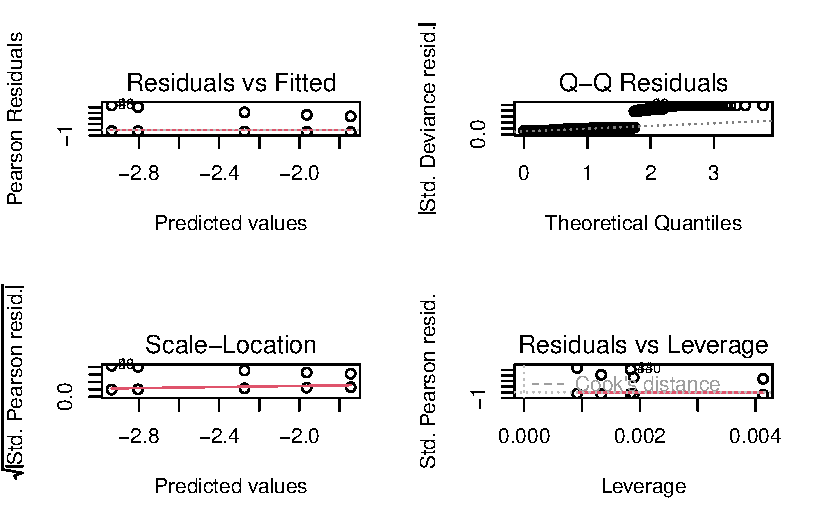
\includegraphics[width=0.85\linewidth,height=\textheight,keepaspectratio]{Section2/Categorical data analysis/Categorical_data_analysis2_files/figure-pdf/unnamed-chunk-14-1.pdf}
\end{center}

\begin{Shaded}
\begin{Highlighting}[]
\CommentTok{\# Determine odds ratio and its 95\% CI (process{-}1)}
\FunctionTok{exp}\NormalTok{(model3}\SpecialCharTok{$}\NormalTok{coefficients) }\CommentTok{\# odds ratio only}
\end{Highlighting}
\end{Shaded}

\begin{verbatim}
#> (Intercept)   agec41-45   agec46-50   agec51-55   agec56-60 
#>  0.06054688  0.87682153  1.70018975  2.31867902  2.88631381
\end{verbatim}

\begin{Shaded}
\begin{Highlighting}[]
\FunctionTok{exp}\NormalTok{(}\FunctionTok{confint}\NormalTok{(model3)) }\CommentTok{\# 95\% CI of odds ratio}
\end{Highlighting}
\end{Shaded}

\begin{verbatim}
#>                 2.5 %     97.5 %
#> (Intercept) 0.0412715 0.08543233
#> agec41-45   0.5613828 1.39311253
#> agec46-50   1.1072235 2.66755273
#> agec51-55   1.4971848 3.66364452
#> agec56-60   1.7402843 4.81378167
\end{verbatim}

\begin{Shaded}
\begin{Highlighting}[]
\FunctionTok{cbind}\NormalTok{(}\AttributeTok{oddsratio=}\FunctionTok{exp}\NormalTok{(model3}\SpecialCharTok{$}\NormalTok{coefficients),}\AttributeTok{CI=}\FunctionTok{exp}\NormalTok{(}\FunctionTok{confint}\NormalTok{(model3))) }\CommentTok{\# odds ratio with 95\% CI}
\end{Highlighting}
\end{Shaded}

\begin{verbatim}
#>              oddsratio     2.5 %     97.5 %
#> (Intercept) 0.06054688 0.0412715 0.08543233
#> agec41-45   0.87682153 0.5613828 1.39311253
#> agec46-50   1.70018975 1.1072235 2.66755273
#> agec51-55   2.31867902 1.4971848 3.66364452
#> agec56-60   2.88631381 1.7402843 4.81378167
\end{verbatim}

\begin{Shaded}
\begin{Highlighting}[]
\CommentTok{\# Determine odds ratio and its 95\% CI (process{-}2)}
\NormalTok{sjPlot}\SpecialCharTok{::}\FunctionTok{tab\_model}\NormalTok{(model3)}
\end{Highlighting}
\end{Shaded}

\begin{longtable}[]{@{}cccc@{}}
\toprule\noalign{}
\endhead
\bottomrule\noalign{}
\endlastfoot
~ & \multicolumn{3}{c@{}}{%
chd 69} \\
Predictors & Odds Ratios & CI & p \\
(Intercept) & 0.06 & 0.04~--~0.09 & \textbf{\textless0.001} \\
agec41-45 & 0.88 & 0.56~--~1.39 & 0.569 \\
agec46-50 & 1.70 & 1.11~--~2.67 & \textbf{0.018} \\
agec51-55 & 2.32 & 1.50~--~3.66 & \textbf{\textless0.001} \\
agec56-60 & 2.89 & 1.74~--~4.81 & \textbf{\textless0.001} \\
Observations & \multicolumn{3}{l@{}}{%
3154} \\
R\textsuperscript{2} Tjur & \multicolumn{3}{l@{}}{%
0.015} \\
\end{longtable}

\begin{Shaded}
\begin{Highlighting}[]
\CommentTok{\# Determine odds ratio and its 95\% CI (process{-}3)}
\NormalTok{gtsummary}\SpecialCharTok{::}\FunctionTok{tbl\_regression}\NormalTok{(model3,}\AttributeTok{exponentiate =}\NormalTok{ T) }\SpecialCharTok{|\textgreater{}}
\NormalTok{  gtsummary}\SpecialCharTok{::}\FunctionTok{as\_hux\_xlsx}\NormalTok{(}\StringTok{"regression\_table.xlsx"}\NormalTok{) }\CommentTok{\# It helps to extract the result to excel}



\CommentTok{\# Determine the AIC, BIC , RMSE of the model}
\NormalTok{performance}\SpecialCharTok{::}\FunctionTok{model\_performance}\NormalTok{(model3)}
\end{Highlighting}
\end{Shaded}

\begin{verbatim}
#> # Indices of model performance
#> 
#> AIC    |   AICc |    BIC | Tjur's R2 |  RMSE | Sigma | Log_loss | Score_log
#> ---------------------------------------------------------------------------
#> 1746.3 | 1746.3 | 1776.6 |     0.015 | 0.272 |     1 |    0.275 |   -21.753
#> 
#> AIC    | Score_spherical |   PCP
#> --------------------------------
#> 1746.3 |           0.006 | 0.853
\end{verbatim}

\begin{Shaded}
\begin{Highlighting}[]
\CommentTok{\# Prediction of new\_data}
\NormalTok{data\_new}\OtherTok{\textless{}{-}}\NormalTok{data[}\FunctionTok{seq}\NormalTok{(}\DecValTok{4}\NormalTok{,}\DecValTok{100}\NormalTok{,}\DecValTok{4}\NormalTok{),]}

\CommentTok{\# predict() function helps to predict the results from in the new data}
\FunctionTok{predict}\NormalTok{(model3,data\_new)}
\end{Highlighting}
\end{Shaded}

\begin{verbatim}
#>         1         2         3         4         5         6         7         8 
#> -1.963340 -2.935789 -1.963340 -1.963340 -2.935789 -1.963340 -1.963340 -2.273598 
#>         9        10        11        12        13        14        15        16 
#> -2.935789 -2.935789 -2.935789 -2.935789 -2.804337 -2.273598 -2.935789 -2.935789 
#>        17        18        19        20        21        22        23        24 
#> -1.963340 -1.963340 -2.273598 -1.963340 -2.273598 -2.273598 -2.273598 -1.963340 
#>        25 
#> -1.963340
\end{verbatim}

\begin{Shaded}
\begin{Highlighting}[]
\CommentTok{\# Add predicted  value to the new data}
\NormalTok{data\_new}\SpecialCharTok{$}\NormalTok{predicted}\OtherTok{\textless{}{-}}\FunctionTok{predict}\NormalTok{(model3,data\_new)}

\CommentTok{\# View head 10 of the data\_new}
\FunctionTok{head}\NormalTok{(data\_new[,}\FunctionTok{c}\NormalTok{(}\DecValTok{1}\SpecialCharTok{:}\DecValTok{11}\NormalTok{,}\DecValTok{23}\NormalTok{)], }\DecValTok{10}\NormalTok{)}
\end{Highlighting}
\end{Shaded}

\begin{verbatim}
#> # A tibble: 10 x 12
#>      age arcus behpat   bmi chd69  chol   dbp dibpat height    id lnsbp
#>    <dbl> <dbl> <chr>  <dbl> <fct> <dbl> <dbl> <fct>   <dbl> <dbl> <dbl>
#>  1    51     1 A1      22.1 No      173    80 Type A     69 22057  4.84
#>  2    41     0 A1      23.0 No      212    84 Type A     70 11389  4.87
#>  3    54     0 A1      23.8 No      214    76 Type A     67 21071  4.77
#>  4    55     1 A1      25.1 No      192    76 Type A     72 13371  4.75
#>  5    44     0 A1      24.4 No      181    80 Type A     72 11249  4.79
#>  6    55     0 A1      26.1 No      185    68 Type A     71  3005  4.70
#>  7    54     0 A1      21.7 No      252    68 Type A     68 12256  4.75
#>  8    46     0 A1      23.9 No      251    74 Type A     74 11358  4.79
#>  9    43     0 A1      25.1 No      213    82 Type A     68 21052  4.80
#> 10    45     0 A1      22.2 No      226    84 Type A     72  3004  4.79
#> # i 1 more variable: predicted <dbl>
\end{verbatim}

\subsection{Interpretation}\label{interpretation-25}

The \texttt{summary(model3)} output reports the log-odds coefficient for
\texttt{agec}, its standard error, z-value, and p-value. Exponentiating
the coefficient (\texttt{exp(model3\$coefficients)}) converts it to an
odds ratio: an OR greater than 1 indicates that CHD (\texttt{chd69})
becomes more likely as age category increases, while an OR less than 1
would indicate lower odds. A 95\% confidence interval
(\texttt{exp(confint(model3))}) that excludes 1 supports a statistically
significant association at the 0.05 level. The \texttt{plot(model3)}
diagnostic panels help check for influential observations and deviance
residual patterns, and \texttt{performance::model\_performance(model3)}
reports fit statistics (AIC, BIC, and pseudo-R²) that are most useful
for comparing this model against alternative specifications rather than
for interpreting in isolation.

\section{\texorpdfstring{\textbf{Multivariable Logistic
regression}}{Multivariable Logistic regression}}\label{multivariable-logistic-regression}

\begin{Shaded}
\begin{Highlighting}[]
\NormalTok{model4}\OtherTok{\textless{}{-}}\FunctionTok{glm}\NormalTok{(}\AttributeTok{formula =}\NormalTok{ chd69}\SpecialCharTok{\textasciitilde{}}\NormalTok{sbp}\SpecialCharTok{+}\NormalTok{agec}\SpecialCharTok{+}\NormalTok{smoke}\SpecialCharTok{+}\NormalTok{bmi,}\AttributeTok{family =} \FunctionTok{binomial}\NormalTok{(}\AttributeTok{link=}\StringTok{"logit"}\NormalTok{),}\AttributeTok{data =}\NormalTok{ data)}
\FunctionTok{summary}\NormalTok{(model4)}
\end{Highlighting}
\end{Shaded}

\begin{verbatim}
#> 
#> Call:
#> glm(formula = chd69 ~ sbp + agec + smoke + bmi, family = binomial(link = "logit"), 
#>     data = data)
#> 
#> Coefficients:
#>              Estimate Std. Error z value Pr(>|z|)    
#> (Intercept) -7.486446   0.739539 -10.123  < 2e-16 ***
#> sbp          0.021540   0.003965   5.433 5.55e-08 ***
#> agec41-45   -0.198522   0.233160  -0.851 0.394523    
#> agec46-50    0.410001   0.226473   1.810 0.070238 .  
#> agec51-55    0.648548   0.232726   2.787 0.005324 ** 
#> agec56-60    0.916249   0.263741   3.474 0.000513 ***
#> smokeYes     0.707014   0.137817   5.130 2.90e-07 ***
#> bmi          0.063477   0.025155   2.523 0.011621 *  
#> ---
#> Signif. codes:  0 '***' 0.001 '**' 0.01 '*' 0.05 '.' 0.1 ' ' 1
#> 
#> (Dispersion parameter for binomial family taken to be 1)
#> 
#>     Null deviance: 1781.2  on 3153  degrees of freedom
#> Residual deviance: 1669.9  on 3146  degrees of freedom
#> AIC: 1685.9
#> 
#> Number of Fisher Scoring iterations: 5
\end{verbatim}

\begin{Shaded}
\begin{Highlighting}[]
\CommentTok{\# Model plots in 2 by 2 arrangement}
\FunctionTok{par}\NormalTok{(}\AttributeTok{mfrow=}\FunctionTok{c}\NormalTok{(}\DecValTok{2}\NormalTok{,}\DecValTok{2}\NormalTok{))}
\FunctionTok{plot}\NormalTok{(model4)}
\end{Highlighting}
\end{Shaded}

\begin{center}
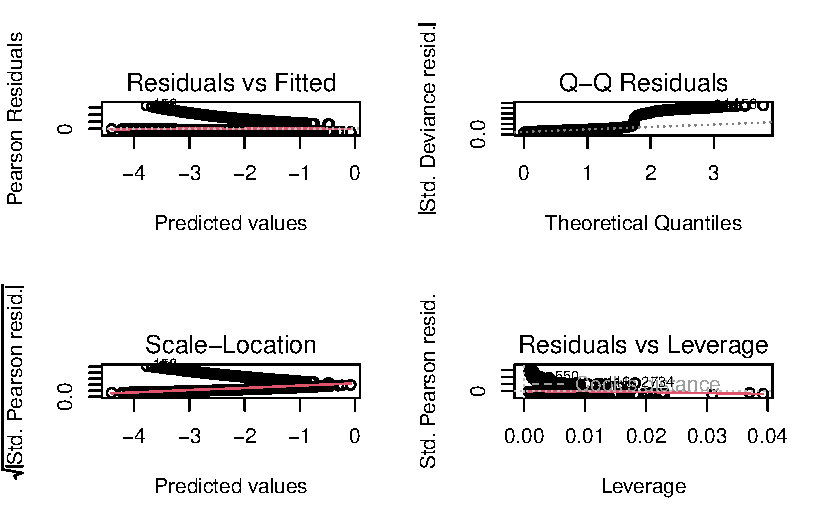
\includegraphics[width=0.85\linewidth,height=\textheight,keepaspectratio]{Section2/Categorical data analysis/Categorical_data_analysis2_files/figure-pdf/unnamed-chunk-15-1.pdf}
\end{center}

\begin{Shaded}
\begin{Highlighting}[]
\CommentTok{\# Determine odds ratio and its 95\% CI (process{-}1)}
\FunctionTok{exp}\NormalTok{(model4}\SpecialCharTok{$}\NormalTok{coefficients) }\CommentTok{\# odds ratio only}
\end{Highlighting}
\end{Shaded}

\begin{verbatim}
#>  (Intercept)          sbp    agec41-45    agec46-50    agec51-55    agec56-60 
#> 0.0005606319 1.0217736501 0.8199414926 1.5068188262 1.9127607823 2.4998947365 
#>     smokeYes          bmi 
#> 2.0279273793 1.0655352259
\end{verbatim}

\begin{Shaded}
\begin{Highlighting}[]
\FunctionTok{exp}\NormalTok{(}\FunctionTok{confint}\NormalTok{(model4)) }\CommentTok{\# 95\% CI of odds ratio}
\end{Highlighting}
\end{Shaded}

\begin{verbatim}
#>                    2.5 %      97.5 %
#> (Intercept) 0.0001308395 0.002381673
#> sbp         1.0137779145 1.029679363
#> agec41-45   0.5226108925 1.307997875
#> agec46-50   0.9752681039 2.376867146
#> agec51-55   1.2215696287 3.051031660
#> agec56-60   1.4915880104 4.210310466
#> smokeYes    1.5511794080 2.664123783
#> bmi         1.0140242588 1.119186342
\end{verbatim}

\begin{Shaded}
\begin{Highlighting}[]
\FunctionTok{cbind}\NormalTok{(}\AttributeTok{oddsratio=}\FunctionTok{exp}\NormalTok{(model4}\SpecialCharTok{$}\NormalTok{coefficients),}\AttributeTok{CI=}\FunctionTok{exp}\NormalTok{(}\FunctionTok{confint}\NormalTok{(model4))) }\CommentTok{\# odds ratio with 95\% CI}
\end{Highlighting}
\end{Shaded}

\begin{verbatim}
#>                oddsratio        2.5 %      97.5 %
#> (Intercept) 0.0005606319 0.0001308395 0.002381673
#> sbp         1.0217736501 1.0137779145 1.029679363
#> agec41-45   0.8199414926 0.5226108925 1.307997875
#> agec46-50   1.5068188262 0.9752681039 2.376867146
#> agec51-55   1.9127607823 1.2215696287 3.051031660
#> agec56-60   2.4998947365 1.4915880104 4.210310466
#> smokeYes    2.0279273793 1.5511794080 2.664123783
#> bmi         1.0655352259 1.0140242588 1.119186342
\end{verbatim}

\begin{Shaded}
\begin{Highlighting}[]
\CommentTok{\# Generate sleek tables from the model and export}
\NormalTok{sjPlot}\SpecialCharTok{::}\FunctionTok{tab\_model}\NormalTok{(model4)}
\end{Highlighting}
\end{Shaded}

\begin{longtable}[]{@{}cccc@{}}
\toprule\noalign{}
\endhead
\bottomrule\noalign{}
\endlastfoot
~ & \multicolumn{3}{c@{}}{%
chd 69} \\
Predictors & Odds Ratios & CI & p \\
(Intercept) & 0.00 & 0.00~--~0.00 & \textbf{\textless0.001} \\
sbp & 1.02 & 1.01~--~1.03 & \textbf{\textless0.001} \\
agec41-45 & 0.82 & 0.52~--~1.31 & 0.395 \\
agec46-50 & 1.51 & 0.98~--~2.38 & 0.070 \\
agec51-55 & 1.91 & 1.22~--~3.05 & \textbf{0.005} \\
agec56-60 & 2.50 & 1.49~--~4.21 & \textbf{0.001} \\
smoke {[}Yes{]} & 2.03 & 1.55~--~2.66 & \textbf{\textless0.001} \\
bmi & 1.07 & 1.01~--~1.12 & \textbf{0.012} \\
Observations & \multicolumn{3}{l@{}}{%
3154} \\
R\textsuperscript{2} Tjur & \multicolumn{3}{l@{}}{%
0.039} \\
\end{longtable}

\begin{Shaded}
\begin{Highlighting}[]
\NormalTok{gtsummary}\SpecialCharTok{::}\FunctionTok{tbl\_regression}\NormalTok{(model4,}\AttributeTok{exponentiate =}\NormalTok{ T) }\SpecialCharTok{|\textgreater{}}
\NormalTok{  gtsummary}\SpecialCharTok{::}\FunctionTok{as\_hux\_xlsx}\NormalTok{(}\StringTok{"regression\_table.xlsx"}\NormalTok{)}

\CommentTok{\# Check model diagnostics}
\NormalTok{performance}\SpecialCharTok{::}\FunctionTok{check\_model}\NormalTok{(model4)}


\CommentTok{\# Determine the AIC, BIC, RMSE of the model}
\NormalTok{performance}\SpecialCharTok{::}\FunctionTok{model\_performance}\NormalTok{(model4)}
\end{Highlighting}
\end{Shaded}

\begin{verbatim}
#> # Indices of model performance
#> 
#> AIC    |   AICc |    BIC | Tjur's R2 |  RMSE | Sigma | Log_loss | Score_log
#> ---------------------------------------------------------------------------
#> 1685.9 | 1685.9 | 1734.3 |     0.039 | 0.268 |     1 |    0.265 |   -22.089
#> 
#> AIC    | Score_spherical |   PCP
#> --------------------------------
#> 1685.9 |           0.004 | 0.856
\end{verbatim}

\begin{Shaded}
\begin{Highlighting}[]
\CommentTok{\# Prediction of new\_data}
\NormalTok{data\_new}\OtherTok{\textless{}{-}}\NormalTok{data[}\FunctionTok{seq}\NormalTok{(}\DecValTok{4}\NormalTok{,}\DecValTok{100}\NormalTok{,}\DecValTok{4}\NormalTok{),]}

\CommentTok{\# predict() function helps to predict the results from in the new data}
\FunctionTok{predict}\NormalTok{(model4,data\_new)}
\end{Highlighting}
\end{Shaded}

\begin{verbatim}
#>         1         2         3         4         5         6         7         8 
#> -2.717921 -2.720629 -2.785170 -2.746757 -3.550708 -2.106103 -2.959220 -2.975913 
#>         9        10        11        12        13        14        15        16 
#> -3.464736 -2.981423 -3.168022 -2.526317 -2.946652 -2.522953 -2.858947 -2.165150 
#>        17        18        19        20        21        22        23        24 
#> -2.781031 -2.350442 -2.244942 -1.915825 -3.056847 -1.675013 -2.197552 -2.204070 
#>        25 
#> -2.038848
\end{verbatim}

\begin{Shaded}
\begin{Highlighting}[]
\CommentTok{\# Add predicted  value to the new data}
\NormalTok{data\_new}\SpecialCharTok{$}\NormalTok{predicted}\OtherTok{\textless{}{-}}\FunctionTok{predict}\NormalTok{(model4,data\_new)}
\end{Highlighting}
\end{Shaded}

\subsection{Interpretation}\label{interpretation-26}

In the multivariable model, each exponentiated coefficient represents
the odds ratio for that predictor holding the other predictors
(\texttt{sbp}, \texttt{agec}, \texttt{smoke}, \texttt{bmi}) constant.
This adjustment is what distinguishes the multivariable estimates from
the crude (unadjusted) odds ratio produced by the univariate model.
\texttt{performance::check\_model(model4)} produces a fuller diagnostic
suite (linearity, homogeneity of variance proxies, influential
observations, and collinearity) than the base \texttt{plot()} method,
and is generally preferred for multivariable models.

\section{\texorpdfstring{\textbf{Interaction in logistic
regression}}{Interaction in logistic regression}}\label{interaction-in-logistic-regression}

An interaction term tests whether the effect of one predictor on the
outcome depends on the level of another predictor. In \texttt{model5},
the term \texttt{sbp*agec} expands to the main effects of \texttt{sbp}
and \texttt{agec} plus their product term (\texttt{sbp:agec}), allowing
the effect of systolic blood pressure on CHD risk to vary across age
categories.

\begin{Shaded}
\begin{Highlighting}[]
\NormalTok{model5}\OtherTok{\textless{}{-}}\FunctionTok{glm}\NormalTok{(}\AttributeTok{formula =}\NormalTok{ chd69}\SpecialCharTok{\textasciitilde{}}\NormalTok{sbp}\SpecialCharTok{*}\NormalTok{agec}\SpecialCharTok{+}\NormalTok{smoke}\SpecialCharTok{+}\NormalTok{bmi,}\AttributeTok{family =} \FunctionTok{binomial}\NormalTok{(}\AttributeTok{link=}\StringTok{"logit"}\NormalTok{),}\AttributeTok{data =}\NormalTok{ data)}
\FunctionTok{summary}\NormalTok{(model5)}
\end{Highlighting}
\end{Shaded}

\begin{verbatim}
#> 
#> Call:
#> glm(formula = chd69 ~ sbp * agec + smoke + bmi, family = binomial(link = "logit"), 
#>     data = data)
#> 
#> Coefficients:
#>                Estimate Std. Error z value Pr(>|z|)    
#> (Intercept)   -4.541067   1.924725  -2.359  0.01831 *  
#> sbp           -0.002297   0.015050  -0.153  0.87868    
#> agec41-45     -3.283702   2.174693  -1.510  0.13105    
#> agec46-50     -2.905318   2.149535  -1.352  0.17650    
#> agec51-55     -2.317372   2.123822  -1.091  0.27521    
#> agec56-60     -3.212210   2.356622  -1.363  0.17286    
#> smokeYes       0.719736   0.138355   5.202 1.97e-07 ***
#> bmi            0.066820   0.025373   2.633  0.00845 ** 
#> sbp:agec41-45  0.024202   0.016989   1.425  0.15428    
#> sbp:agec46-50  0.025912   0.016763   1.546  0.12214    
#> sbp:agec51-55  0.023324   0.016507   1.413  0.15766    
#> sbp:agec56-60  0.031794   0.018064   1.760  0.07838 .  
#> ---
#> Signif. codes:  0 '***' 0.001 '**' 0.01 '*' 0.05 '.' 0.1 ' ' 1
#> 
#> (Dispersion parameter for binomial family taken to be 1)
#> 
#>     Null deviance: 1781.2  on 3153  degrees of freedom
#> Residual deviance: 1666.4  on 3142  degrees of freedom
#> AIC: 1690.4
#> 
#> Number of Fisher Scoring iterations: 6
\end{verbatim}

\begin{Shaded}
\begin{Highlighting}[]
\CommentTok{\# Odds ratio and 95\% CI}
\FunctionTok{exp}\NormalTok{(model5}\SpecialCharTok{$}\NormalTok{coefficients)}
\end{Highlighting}
\end{Shaded}

\begin{verbatim}
#>   (Intercept)           sbp     agec41-45     agec46-50     agec51-55 
#>    0.01066203    0.99770539    0.03748920    0.05473139    0.09853220 
#>     agec56-60      smokeYes           bmi sbp:agec41-45 sbp:agec46-50 
#>    0.04026753    2.05389046    1.06910320    1.02449693    1.02625110 
#> sbp:agec51-55 sbp:agec56-60 
#>    1.02359811    1.03230533
\end{verbatim}

\begin{Shaded}
\begin{Highlighting}[]
\FunctionTok{exp}\NormalTok{(}\FunctionTok{confint}\NormalTok{(model5))}
\end{Highlighting}
\end{Shaded}

\begin{verbatim}
#>                      2.5 %    97.5 %
#> (Intercept)   0.0002646532 0.5152048
#> sbp           0.9673878390 1.0264165
#> agec41-45     0.0004896772 2.5299152
#> agec46-50     0.0007409633 3.4623276
#> agec51-55     0.0013989779 5.9060431
#> agec56-60     0.0003618415 3.8041663
#> smokeYes      1.5695268215 2.7012457
#> bmi           1.0170134637 1.1234531
#> sbp:agec41-45 0.9916460076 1.0602057
#> sbp:agec46-50 0.9939356825 1.0616798
#> sbp:agec51-55 0.9919077874 1.0584460
#> sbp:agec56-60 0.9971848540 1.0705886
\end{verbatim}

\begin{Shaded}
\begin{Highlighting}[]
\FunctionTok{cbind}\NormalTok{(}\AttributeTok{oddsratio=}\FunctionTok{exp}\NormalTok{(model5}\SpecialCharTok{$}\NormalTok{coefficients),}\AttributeTok{CI=}\FunctionTok{exp}\NormalTok{(}\FunctionTok{confint}\NormalTok{(model5)))}
\end{Highlighting}
\end{Shaded}

\begin{verbatim}
#>                oddsratio        2.5 %    97.5 %
#> (Intercept)   0.01066203 0.0002646532 0.5152048
#> sbp           0.99770539 0.9673878390 1.0264165
#> agec41-45     0.03748920 0.0004896772 2.5299152
#> agec46-50     0.05473139 0.0007409633 3.4623276
#> agec51-55     0.09853220 0.0013989779 5.9060431
#> agec56-60     0.04026753 0.0003618415 3.8041663
#> smokeYes      2.05389046 1.5695268215 2.7012457
#> bmi           1.06910320 1.0170134637 1.1234531
#> sbp:agec41-45 1.02449693 0.9916460076 1.0602057
#> sbp:agec46-50 1.02625110 0.9939356825 1.0616798
#> sbp:agec51-55 1.02359811 0.9919077874 1.0584460
#> sbp:agec56-60 1.03230533 0.9971848540 1.0705886
\end{verbatim}

\begin{tcolorbox}[enhanced jigsaw, bottomrule=.15mm, breakable, opacityback=0, toptitle=1mm, titlerule=0mm, bottomtitle=1mm, colback=white, arc=.35mm, rightrule=.15mm, toprule=.15mm, leftrule=.75mm, title=\textcolor{quarto-callout-tip-color}{\faLightbulb}\hspace{0.5em}{Tip}, colbacktitle=quarto-callout-tip-color!10!white, colframe=quarto-callout-tip-color-frame, coltitle=black, left=2mm, opacitybacktitle=0.6]

When an interaction term is included, the main-effect odds ratios for
\texttt{sbp} and \texttt{agec} no longer have a simple standalone
interpretation --- they represent the effect only when the other
interacting variable is held at its reference level (or zero). To
interpret the joint effect, compute the combined odds ratio at specific,
meaningful combinations of both variables (e.g., using the
\texttt{emmeans} or \texttt{ggeffects} packages), or test whether the
interaction coefficient itself is statistically significant.

\end{tcolorbox}

\textbf{Interpretation:} A significant p-value for the \texttt{sbp:agec}
interaction term indicates that the relationship between systolic blood
pressure and CHD risk differs across age categories, and the model
should be interpreted and reported with that interaction in mind rather
than through separate main-effect odds ratios.

\chapter{Extension of Logistic
regression}\label{extension-of-logistic-regression}

There are multiple extensions of logistic regression. Some of them are
as follows:

\begin{enumerate}
\def\labelenumi{\arabic{enumi}.}
\tightlist
\item
  Exact logistic regression
\item
  Firth Penalization logistic regression
\item
  Generalized estimating equation
\item
  Multinomial logistic regression
\item
  Ordinal logistic regression
\end{enumerate}

The details of each type of logistic regression are given below:

\section{Exact logistic regression}\label{exact-logistic-regression}

Exact logistic regression is an extension of logistic regression in
which log odds of the binary outcome is modeled as a linear combination
of the predictor variables. It is used in the following situations:

\begin{enumerate}
\def\labelenumi{\arabic{enumi}.}
\tightlist
\item
  When the sample size is too small for a regular logistic regression
  (which uses the standard maximum-likelihood-based estimator)
\item
  When some of the cells formed by the outcome and categorical predictor
  variable have zero observations.
\item
  When sample size is adequate but the event is rare (sparse data)
\end{enumerate}

The estimates given by exact logistic regression do not depend on
asymptotic results.

Lets take a dataset and work on it

\begin{Shaded}
\begin{Highlighting}[]
\NormalTok{dat }\OtherTok{\textless{}{-}} \FunctionTok{read.table}\NormalTok{(}\AttributeTok{text =} \StringTok{"}
\StringTok{SN Complication Procedure}
\StringTok{1 Yes Old}
\StringTok{2 Yes Old}
\StringTok{3 Yes Old}
\StringTok{4 Yes Old}
\StringTok{5 Yes Old}
\StringTok{6 No New}
\StringTok{7 No New}
\StringTok{8 No New}
\StringTok{9 No New}
\StringTok{10 No New}
\StringTok{11 No New}
\StringTok{12 No New}
\StringTok{13 No New}
\StringTok{14 No New}
\StringTok{15 No New}
\StringTok{16 No New}
\StringTok{17 No New}
\StringTok{18 No New}
\StringTok{19 No New}
\StringTok{20 No New}
\StringTok{21 No New}
\StringTok{22 No New}
\StringTok{23 No New}
\StringTok{24 No New}
\StringTok{25 No New}
\StringTok{26 No New}
\StringTok{27 No New}
\StringTok{28 No New}
\StringTok{29 No New}
\StringTok{31 No New}
\StringTok{32 No New}
\StringTok{33 No New}
\StringTok{34 No New}
\StringTok{35 No New}
\StringTok{36 No New}
\StringTok{37 No Old}
\StringTok{38 No Old}
\StringTok{39 No Old}
\StringTok{40 No Old}
\StringTok{41 No Old}
\StringTok{42 No Old}
\StringTok{43 No Old}
\StringTok{44 No Old}
\StringTok{45 No Old}
\StringTok{46 No Old}
\StringTok{47 No Old}
\StringTok{48 No Old}
\StringTok{49 No Old}
\StringTok{50 No Old}
\StringTok{51 No Old}
\StringTok{52 No Old}
\StringTok{53 No Old}
\StringTok{54 No Old}
\StringTok{55 No Old}
\StringTok{56 No Old}
\StringTok{57 No Old}
\StringTok{58 No Old}
\StringTok{59 No Old}
\StringTok{60 No Old}
\StringTok{61 No Old}
\StringTok{"}\NormalTok{, }\AttributeTok{header =} \ConstantTok{TRUE}\NormalTok{, }\AttributeTok{stringsAsFactors =} \ConstantTok{FALSE}\NormalTok{)}
\end{Highlighting}
\end{Shaded}

Lets generate a table between complication and procedure in the dataset.

\begin{Shaded}
\begin{Highlighting}[]
\FunctionTok{table}\NormalTok{(dat}\SpecialCharTok{$}\NormalTok{Complication, dat}\SpecialCharTok{$}\NormalTok{Procedure)}
\end{Highlighting}
\end{Shaded}

\begin{verbatim}
#>      
#>       New Old
#>   No   30  25
#>   Yes   0   5
\end{verbatim}

Code for exact logistic regression in R

\begin{Shaded}
\begin{Highlighting}[]
\CommentTok{\# Prepare data}
\NormalTok{dat1 }\OtherTok{\textless{}{-}} \FunctionTok{data.frame}\NormalTok{(}\AttributeTok{procedure =} \FunctionTok{c}\NormalTok{(}\StringTok{"New"}\NormalTok{, }\StringTok{"Old"}\NormalTok{), }\AttributeTok{complication =} \FunctionTok{c}\NormalTok{(}\DecValTok{0}\NormalTok{, }\DecValTok{5}\NormalTok{), }\AttributeTok{ntrials =} \FunctionTok{c}\NormalTok{(}\DecValTok{30}\NormalTok{, }\DecValTok{30}\NormalTok{))}
\NormalTok{dat1}\SpecialCharTok{$}\NormalTok{procedure }\OtherTok{\textless{}{-}} \FunctionTok{factor}\NormalTok{(dat1}\SpecialCharTok{$}\NormalTok{procedure, }\AttributeTok{levels =}\FunctionTok{c}\NormalTok{(}\StringTok{"Old"}\NormalTok{, }\StringTok{"New"}\NormalTok{), }\AttributeTok{labels=}\FunctionTok{c}\NormalTok{(}\StringTok{"Old"}\NormalTok{, }\StringTok{"New"}\NormalTok{) )  }\CommentTok{\# Ensure \textquotesingle{}procedure\textquotesingle{} is a factor}

\CommentTok{\# Fit the empirical logistic regression model}
\NormalTok{model }\OtherTok{\textless{}{-}} \FunctionTok{elrm}\NormalTok{(}\AttributeTok{formula =}\NormalTok{ complication}\SpecialCharTok{/}\NormalTok{ntrials }\SpecialCharTok{\textasciitilde{}}\NormalTok{ procedure, }\AttributeTok{r=}\DecValTok{2}\NormalTok{,}
               \AttributeTok{interest =} \SpecialCharTok{\textasciitilde{}}\NormalTok{procedure, }
               \AttributeTok{iter =} \DecValTok{22000}\NormalTok{, }
               \AttributeTok{dataset =}\NormalTok{ dat1, }
               \AttributeTok{burnIn =} \DecValTok{2000}\NormalTok{)}

\CommentTok{\# Summarize the results}
\FunctionTok{summary}\NormalTok{(model)}
\end{Highlighting}
\end{Shaded}

In exact logistic regression there is complete separation, we have to
use firth penalized method.

\section{Firth Penalized Method}\label{firth-penalized-method}

It is a simple solution that can mitigate the bias caused by rare events
in a dataset. It is applicable in the case of complete separation.
Complete separation or perfect separation is the condition where one
covariate/explanatory variable always or never occurs with the event of
interest or outcome variable. It is seen most often when the event is
rare, but it can also occur in non-rare events and even in large
datasets. The evidence of complete separation includes:

\begin{enumerate}
\def\labelenumi{\arabic{enumi}.}
\item
  Infinite estimates
\item
  Large standard error
\item
  Poor fit
\end{enumerate}

Firth logistic regression can be employed to handle complete separation
by introducing penalty terms. It is more robust than traditional
logistic regression in the presence of rare events or small sample
sizes.

In order to use this in R, we can use logistf package, which includes
the \texttt{logistf()} function.

\begin{Shaded}
\begin{Highlighting}[]
\FunctionTok{library}\NormalTok{(logistf)}

\CommentTok{\# prepare data }
\NormalTok{dat}\SpecialCharTok{$}\NormalTok{Complication}\OtherTok{\textless{}{-}}\FunctionTok{as.factor}\NormalTok{(dat}\SpecialCharTok{$}\NormalTok{Complication)}
\NormalTok{dat}\SpecialCharTok{$}\NormalTok{Procedure}\OtherTok{\textless{}{-}}\FunctionTok{as.factor}\NormalTok{(dat}\SpecialCharTok{$}\NormalTok{Procedure)}
\NormalTok{model }\OtherTok{\textless{}{-}} \FunctionTok{logistf}\NormalTok{(Complication}\SpecialCharTok{\textasciitilde{}}\NormalTok{Procedure,}\AttributeTok{data =}\NormalTok{ dat)}

\FunctionTok{summary}\NormalTok{(model)}
\end{Highlighting}
\end{Shaded}

\begin{verbatim}
#> logistf(formula = Complication ~ Procedure, data = dat)
#> 
#> Model fitted by Penalized ML
#> Coefficients:
#>                   coef se(coef) lower 0.95 upper 0.95     Chisq            p
#> (Intercept)  -4.110874 1.425754 -8.9524616  -2.153841 37.856099 7.615991e-10
#> ProcedureOld  2.576944 1.501269  0.3247434   7.472101  5.322758 2.104867e-02
#>              method
#> (Intercept)       2
#> ProcedureOld      2
#> 
#> Method: 1-Wald, 2-Profile penalized log-likelihood, 3-None
#> 
#> Likelihood ratio test=5.322758 on 1 df, p=0.02104867, n=60
#> Wald test = 18.95857 on 1 df, p = 1.335876e-05
\end{verbatim}

\begin{Shaded}
\begin{Highlighting}[]
\NormalTok{sjPlot}\SpecialCharTok{::}\FunctionTok{tab\_model}\NormalTok{(model)}
\end{Highlighting}
\end{Shaded}

\begin{longtable}[]{@{}cccc@{}}
\toprule\noalign{}
\endhead
\bottomrule\noalign{}
\endlastfoot
~ & \multicolumn{3}{c@{}}{%
Complication} \\
Predictors & Odds Ratios & CI & p \\
(Intercept) & 0.02 & 0.00~--~0.27 & \textbf{\textless0.001} \\
Procedure {[}Old{]} & 13.16 & 0.69~--~249.48 & \textbf{0.021} \\
Observations & \multicolumn{3}{l@{}}{%
60} \\
R\textsuperscript{2} & \multicolumn{3}{l@{}}{%
0.088} \\
\end{longtable}

\section{Generalized Estimating Equations
(GEE)}\label{generalized-estimating-equations-gee}

\subsection{Introduction}\label{introduction-5}

Generalized Estimating Equations (GEE) extend the generalized linear
model to correlated or clustered data, such as repeated measurements on
the same subject over time, or observations nested within clusters
(e.g., patients within clinics). Standard logistic regression assumes
independent observations; when that assumption is violated, ignoring the
correlation produces standard errors that are too small (or occasionally
too large), leading to incorrect inference even though the coefficient
estimates themselves may remain roughly unbiased.

GEE addresses this by specifying a \textbf{working correlation
structure} (e.g., independence, exchangeable, autoregressive AR(1), or
unstructured) for the repeated observations within a cluster, and then
uses a robust ``sandwich'' variance estimator that gives valid standard
errors even if the working correlation structure is misspecified.

Unlike mixed-effects (random-effects) models, which give
subject-specific (``conditional'') interpretations, GEE coefficients
have a \textbf{population-averaged} interpretation: the odds ratio
reflects the average effect of a predictor across the population,
marginal over the repeated measurements.

\subsection{When to use GEE}\label{when-to-use-gee}

\begin{enumerate}
\def\labelenumi{\arabic{enumi}.}
\tightlist
\item
  The outcome is measured repeatedly on the same subjects (longitudinal
  data) or subjects are clustered (e.g., by clinic, family, or region).
\item
  The scientific question concerns the population-averaged effect of
  predictors rather than subject-specific effects.
\item
  The primary interest is in correct standard errors and hypothesis
  tests rather than in modeling between-subject variability directly.
\end{enumerate}

\subsection{Fitting a GEE model in R}\label{fitting-a-gee-model-in-r}

We use the \texttt{geepack} package, which provides the
\texttt{geeglm()} function. We will use the classic \texttt{respiratory}
dataset included with \texttt{geepack}: a multi-center clinical trial in
which patients were followed over four visits, with a binary respiratory
status outcome recorded at each visit (clustered by patient
\texttt{id}).

\begin{Shaded}
\begin{Highlighting}[]
\FunctionTok{library}\NormalTok{(geepack)}

\CommentTok{\# load the built{-}in respiratory dataset (repeated measures per patient)}
\FunctionTok{data}\NormalTok{(respiratory)}
\FunctionTok{head}\NormalTok{(respiratory)}
\end{Highlighting}
\end{Shaded}

\begin{verbatim}
#>   center id treat sex age baseline visit outcome
#> 1      1  1     P   M  46        0     1       0
#> 2      1  1     P   M  46        0     2       0
#> 3      1  1     P   M  46        0     3       0
#> 4      1  1     P   M  46        0     4       0
#> 5      1  2     P   M  28        0     1       0
#> 6      1  2     P   M  28        0     2       0
\end{verbatim}

\begin{Shaded}
\begin{Highlighting}[]
\CommentTok{\# Fit a GEE logistic model with an exchangeable working correlation,}
\CommentTok{\# since repeated visits within the same patient are correlated}
\NormalTok{gee\_model }\OtherTok{\textless{}{-}} \FunctionTok{geeglm}\NormalTok{(outcome }\SpecialCharTok{\textasciitilde{}}\NormalTok{ treat }\SpecialCharTok{+}\NormalTok{ sex }\SpecialCharTok{+}\NormalTok{ baseline }\SpecialCharTok{+}\NormalTok{ age,}
                     \AttributeTok{id =}\NormalTok{ id,}
                     \AttributeTok{data =}\NormalTok{ respiratory,}
                     \AttributeTok{family =} \FunctionTok{binomial}\NormalTok{(}\AttributeTok{link =} \StringTok{"logit"}\NormalTok{),}
                     \AttributeTok{corstr =} \StringTok{"exchangeable"}\NormalTok{)}

\NormalTok{gee\_model\_summary}\OtherTok{\textless{}{-}}\FunctionTok{summary}\NormalTok{(gee\_model)}

\CommentTok{\# Odds ratio and 95\% CI}
\NormalTok{coef\_est }\OtherTok{\textless{}{-}}\NormalTok{ gee\_model\_summary}\SpecialCharTok{$}\NormalTok{coefficients[, }\StringTok{"Estimate"}\NormalTok{]}
\NormalTok{se }\OtherTok{\textless{}{-}}\NormalTok{ gee\_model\_summary}\SpecialCharTok{$}\NormalTok{coefficients[, }\StringTok{"Std.err"}\NormalTok{]}

\NormalTok{lower }\OtherTok{\textless{}{-}}\NormalTok{ coef\_est }\SpecialCharTok{{-}} \FloatTok{1.96} \SpecialCharTok{*}\NormalTok{ se}
\NormalTok{upper }\OtherTok{\textless{}{-}}\NormalTok{ coef\_est }\SpecialCharTok{+} \FloatTok{1.96} \SpecialCharTok{*}\NormalTok{ se}

\NormalTok{CI }\OtherTok{\textless{}{-}} \FunctionTok{cbind}\NormalTok{(}\AttributeTok{Estimate =}\NormalTok{ coef\_est,}
            \AttributeTok{Lower95 =}\NormalTok{ lower,}
            \AttributeTok{Upper95 =}\NormalTok{ upper)}

\FunctionTok{exp}\NormalTok{(CI)}
\end{Highlighting}
\end{Shaded}

\begin{verbatim}
#>       Estimate   Lower95    Upper95
#> [1,] 2.1091310 0.5226750  8.5108980
#> [2,] 0.2772380 0.1393793  0.5514513
#> [3,] 0.7623601 0.3329734  1.7454632
#> [4,] 7.3645242 3.8773182 13.9880747
#> [5,] 0.9863820 0.9609202  1.0125184
\end{verbatim}

\begin{tcolorbox}[enhanced jigsaw, bottomrule=.15mm, breakable, opacityback=0, toptitle=1mm, titlerule=0mm, bottomtitle=1mm, colback=white, arc=.35mm, rightrule=.15mm, toprule=.15mm, leftrule=.75mm, title=\textcolor{quarto-callout-tip-color}{\faLightbulb}\hspace{0.5em}{Tip}, colbacktitle=quarto-callout-tip-color!10!white, colframe=quarto-callout-tip-color-frame, coltitle=black, left=2mm, opacitybacktitle=0.6]

Model comparison statistics such as AIC/BIC are not defined for GEE
models in the usual likelihood-based sense (GEE is estimated via
quasi-likelihood, not full likelihood). Use the QIC (Quasi-likelihood
under the Independence model Criterion) instead, available via
\texttt{MuMIn::QIC()} or \texttt{geepack::QIC()} depending on package
version, to compare working correlation structures or nested predictor
sets.

\end{tcolorbox}

\textbf{Interpretation:} The exponentiated coefficients from
\texttt{gee\_model} are population-averaged odds ratios. For example,
the odds ratio for \texttt{treat} represents how much more (or less)
likely a patient is to have the outcome of interest under the active
treatment versus control, averaged across the population and adjusted
for \texttt{sex}, \texttt{baseline} status, and \texttt{age}, while
accounting for the within-patient correlation across the four visits.

\section{Multinomial Logistic regression
Analysis}\label{multinomial-logistic-regression-analysis}

\subsection{Introduction}\label{introduction-6}

It is the extension of the logistic regression model to accommodate a
categorical outcome variable that has more than two categories. The
multinomial logistic regression model for an outcome variable with G
levels is as follows:

\[ ln(\frac{P(Y=g|X)} {P(Y=0|X)}) = \alpha_k + \beta_1 X_1 +\beta_2X_2 +\beta_3X_3 +\dots +\beta_gX_g \]

where g =1, 2, 3,\ldots{} G-1

X are the independent variables

If there are n categories in the outcome variable, then there will be
n-1 odds like ratio comparing with one reference group to each of the
other categories.

The exponentiated coefficient obtained from multinomial logistic
regression is not a true odds ratio in the classical sense --- it is an
``odds-like'' ratio comparing category \emph{g} to the reference
category, since it does not meet the strict definition of odds (ratio of
success to failure) that applies to a two-category outcome.

\subsection{Assumptions}\label{assumptions-1}

\begin{itemize}
\item
  It assumes the outcome variable as nominal
\item
  It doesn't account ordering in the outcome variables
\end{itemize}

For the demonstration of multinomial logistic regression analysis, we
will be using data from NDHS 2021. The sample data used can be
downloaded from the
\href{https://drive.google.com/file/d/10ZTS_xTzaG432oBly6OFp2PvHBOgOpfO}{link
here}. The list of variables are as follows:

\begin{itemize}
\item
  \texttt{Combined2\_1}: It is the outcome variable with four levels:
  Normal/Anemia only/Undernutrition Only/Coexistence
\item
  \texttt{Wealth\_quintile}: Wealth quintile
\item
  \texttt{motheredu} : Mother's education
\item
  \texttt{housedecision}: Mother's participation in household decision
  making
\item
  \texttt{health\_program}: Exposure of mother to health related program
  in TV/radio
\item
  \texttt{age2}: Age of child
\item
  \texttt{Sex}: Sex of child
\item
  \texttt{Place\_of\_residence}: Place of residence of child
\item
  \texttt{fatheredu}: Father's education level
\item
  \texttt{Ecological\_region}: Ecological belt
\item
  \texttt{parity}: Parity
\item
  \texttt{maternal\_nut}: Mother's nutritional status
\item
  \texttt{nt\_wm\_any\_anem}: Mother's anemia status
\end{itemize}

\begin{Shaded}
\begin{Highlighting}[]
\CommentTok{\# load dataset}
\NormalTok{dt}\OtherTok{\textless{}{-}}\FunctionTok{readRDS}\NormalTok{(}\StringTok{"D:/Epi Biostat with R/Biostat\_with\_R/Section2/Categorical data analysis/Datasets/dt.RDS"}\NormalTok{)}

\CommentTok{\# load libraries}
\FunctionTok{library}\NormalTok{(nnet) }\CommentTok{\# "multinom()" function is from nnet}
\FunctionTok{library}\NormalTok{(sjPlot) }\CommentTok{\# to make ready{-}made tables and charts}
\FunctionTok{library}\NormalTok{(ggeffects) }\CommentTok{\# to plot models}
\FunctionTok{library}\NormalTok{(performance) }\CommentTok{\# to check assumptions}
\end{Highlighting}
\end{Shaded}

The code to use multinomial logistic regression is as follows:

\begin{Shaded}
\begin{Highlighting}[]
\NormalTok{mdel1}\OtherTok{\textless{}{-}}\FunctionTok{multinom}\NormalTok{(}\AttributeTok{formula =}\NormalTok{ Combined2\_1}\SpecialCharTok{\textasciitilde{}}\NormalTok{Wealth\_quintile}\SpecialCharTok{+}\NormalTok{motheredu}\SpecialCharTok{+}\NormalTok{housedecision}\SpecialCharTok{+}\NormalTok{health\_program}\SpecialCharTok{+}\NormalTok{age2}\SpecialCharTok{+}\NormalTok{Sex}\SpecialCharTok{+}\NormalTok{Place\_of\_residence}\SpecialCharTok{+}\NormalTok{fatheredu}\SpecialCharTok{+}\NormalTok{Ecological\_region}\SpecialCharTok{+}\NormalTok{parity}\SpecialCharTok{+}\NormalTok{maternal\_nut}\SpecialCharTok{+}\NormalTok{nt\_wm\_any\_anem, }\AttributeTok{data=}\NormalTok{dt)}
\end{Highlighting}
\end{Shaded}

\begin{verbatim}
#> # weights:  92 (66 variable)
#> initial  value 2617.323754 
#> iter  10 value 2356.751620
#> iter  20 value 2310.420979
#> iter  30 value 2290.536865
#> iter  40 value 2289.133329
#> iter  50 value 2289.050213
#> final  value 2289.046139 
#> converged
\end{verbatim}

\begin{Shaded}
\begin{Highlighting}[]
\FunctionTok{summary}\NormalTok{(mdel1)}
\end{Highlighting}
\end{Shaded}

\begin{verbatim}
#> Call:
#> multinom(formula = Combined2_1 ~ Wealth_quintile + motheredu + 
#>     housedecision + health_program + age2 + Sex + Place_of_residence + 
#>     fatheredu + Ecological_region + parity + maternal_nut + nt_wm_any_anem, 
#>     data = dt)
#> 
#> Coefficients:
#>                     (Intercept) Wealth_quintilepoorer Wealth_quintilemiddle
#> Anemia only           0.9854172          -0.010407023            0.04834015
#> Undernutrition only  -0.6477979          -0.003986444           -0.09799603
#> Coexistence           0.5766046          -0.184151862           -0.44344604
#>                     Wealth_quintilericher Wealth_quintilerichest
#> Anemia only                   -0.04228353             -0.6770043
#> Undernutrition only           -0.74235271             -0.8526707
#> Coexistence                   -0.67105714             -0.8768949
#>                     motheredubasic  mothereduSecondary and Higher
#> Anemia only              0.01146830                     0.1501191
#> Undernutrition only      0.04965992                    -0.1225593
#> Coexistence             -0.33018654                    -0.6422108
#>                     housedecisionParticipation health_programYes
#> Anemia only                         -0.3730769       -0.06091002
#> Undernutrition only                 -0.3526384       -0.13557889
#> Coexistence                         -0.3383432       -0.04715707
#>                     age213-36 months age237-59 months   Sexfemale
#> Anemia only               -1.0851727        -2.003195 -0.08409981
#> Undernutrition only        1.2476138         1.258172 -0.03024442
#> Coexistence               -0.4089829        -1.507620 -0.09316537
#>                     Place_of_residencerural fatheredubasic 
#> Anemia only                     -0.15613950      -0.1946993
#> Undernutrition only              0.02617873      -0.1095205
#> Coexistence                      0.17811935      -0.1783381
#>                     fathereduSecondary and Higher Ecological_regionhill
#> Anemia only                           -0.46807421            -0.3138077
#> Undernutrition only                   -0.17365568            -0.5792796
#> Coexistence                           -0.04204977            -0.7531653
#>                     Ecological_regionterai parityPrimipara parityMultipara
#> Anemia only                     0.26819046      0.42232303      0.56309415
#> Undernutrition only            -0.41830902     -0.58313145     -0.06466644
#> Coexistence                    -0.08372189      0.02709827      0.54950630
#>                     maternal_nutOverwt obese maternal_nutthin nt_wm_any_anemYes
#> Anemia only                       0.26594352       0.05020825         0.4621247
#> Undernutrition only              -0.02098865       0.38562048         0.2059181
#> Coexistence                      -0.04115914       0.42109672         0.7761082
#> 
#> Std. Errors:
#>                     (Intercept) Wealth_quintilepoorer Wealth_quintilemiddle
#> Anemia only           0.2738739             0.1919641             0.2066312
#> Undernutrition only   0.3659968             0.1960567             0.2182094
#> Coexistence           0.3018701             0.2168357             0.2463465
#>                     Wealth_quintilericher Wealth_quintilerichest
#> Anemia only                     0.2241009              0.2650318
#> Undernutrition only             0.2682186              0.3096395
#> Coexistence                     0.2798183              0.3337100
#>                     motheredubasic  mothereduSecondary and Higher
#> Anemia only               0.1920722                     0.2144264
#> Undernutrition only       0.1932469                     0.2245962
#> Coexistence               0.2024112                     0.2389557
#>                     housedecisionParticipation health_programYes
#> Anemia only                          0.1543438         0.1500803
#> Undernutrition only                  0.1691325         0.1616194
#> Coexistence                          0.1769248         0.1825790
#>                     age213-36 months age237-59 months Sexfemale
#> Anemia only                0.1925852        0.2021013 0.1234745
#> Undernutrition only        0.4180860        0.4161420 0.1337545
#> Coexistence                0.2395562        0.2545531 0.1457525
#>                     Place_of_residencerural fatheredubasic 
#> Anemia only                       0.1327872       0.2443898
#> Undernutrition only               0.1433533       0.2504912
#> Coexistence                       0.1561835       0.2601701
#>                     fathereduSecondary and Higher Ecological_regionhill
#> Anemia only                             0.2631055             0.2567353
#> Undernutrition only                     0.2718673             0.2344684
#> Coexistence                             0.2836707             0.2598943
#>                     Ecological_regionterai parityPrimipara parityMultipara
#> Anemia only                      0.2812538       0.1620888       0.1447750
#> Undernutrition only              0.2706417       0.2100337       0.1914079
#> Coexistence                      0.2953945       0.1865385       0.1633622
#>                     maternal_nutOverwt obese maternal_nutthin nt_wm_any_anemYes
#> Anemia only                        0.1581779        0.1923029         0.1369080
#> Undernutrition only                0.1815454        0.1968095         0.1520609
#> Coexistence                        0.2090812        0.2022801         0.1574196
#> 
#> Residual Deviance: 4578.092 
#> AIC: 4704.092
\end{verbatim}

In order to check assumptions of the model we can use performance
package.

\begin{Shaded}
\begin{Highlighting}[]
\CommentTok{\# check for multi{-}collinearity}
\NormalTok{performance}\SpecialCharTok{::}\FunctionTok{check\_collinearity}\NormalTok{(mdel1)}
\end{Highlighting}
\end{Shaded}

\begin{verbatim}
#> # Check for Multicollinearity
#> 
#> Low Correlation
#> 
#>               Term     VIF VIF 95% CI adj. VIF Tolerance Tolerance 95% CI
#>      housedecision  -14.21                         -0.07                 
#>     health_program   -1.70                         -0.59                 
#>               age2  -11.44                         -0.09                 
#>                Sex   -5.11                         -0.20                 
#>          fatheredu -124.78                     -8.01e-03                 
#>  Ecological_region  -57.09                         -0.02                 
#>             parity -205.04                     -4.88e-03                 
#>       maternal_nut   -1.22                         -0.82                 
#>     nt_wm_any_anem  -16.32                         -0.06                 
#> 
#> Moderate Correlation
#> 
#>                Term  VIF     VIF 95% CI adj. VIF Tolerance Tolerance 95% CI
#>           motheredu 5.10 [ 4.71,  5.52]     2.26      0.20     [0.18, 0.21]
#>  Place_of_residence 7.91 [ 7.30,  8.59]     2.81      0.13     [0.12, 0.14]
#> 
#> High Correlation
#> 
#>             Term   VIF     VIF 95% CI adj. VIF Tolerance Tolerance 95% CI
#>  Wealth_quintile 38.58 [35.41, 42.04]     6.21      0.03     [0.02, 0.03]
\end{verbatim}

We can use \texttt{tab\_model()} from the sjPlot package to make a
ready-made table and \texttt{plot\_model()} from sjPlot to create a
sleek chart.

\begin{Shaded}
\begin{Highlighting}[]
\CommentTok{\# readymade table}
\FunctionTok{tab\_model}\NormalTok{(mdel1)}
\end{Highlighting}
\end{Shaded}

\begin{longtable}[]{@{}
  >{\centering\arraybackslash}p{(\linewidth - 8\tabcolsep) * \real{0.2000}}
  >{\centering\arraybackslash}p{(\linewidth - 8\tabcolsep) * \real{0.2000}}
  >{\centering\arraybackslash}p{(\linewidth - 8\tabcolsep) * \real{0.2000}}
  >{\centering\arraybackslash}p{(\linewidth - 8\tabcolsep) * \real{0.2000}}
  >{\centering\arraybackslash}p{(\linewidth - 8\tabcolsep) * \real{0.2000}}@{}}
\toprule\noalign{}
\endhead
\bottomrule\noalign{}
\endlastfoot
~ &
\multicolumn{4}{>{\centering\arraybackslash}p{(\linewidth - 8\tabcolsep) * \real{0.8000} + 6\tabcolsep}@{}}{%
Combined 2 1} \\
Predictors & Odds Ratios & CI & p & Response \\
(Intercept) & 2.68 & 1.57~--~4.58 & \textbf{\textless0.001} & Anemia
only \\
\begin{minipage}[t]{\linewidth}\raggedright
wealth index combined:\\
poorer\strut
\end{minipage} & 0.99 & 0.68~--~1.44 & 0.957 & Anemia only \\
\begin{minipage}[t]{\linewidth}\raggedright
wealth index combined:\\
middle\strut
\end{minipage} & 1.05 & 0.70~--~1.57 & 0.815 & Anemia only \\
\begin{minipage}[t]{\linewidth}\raggedright
wealth index combined:\\
richer\strut
\end{minipage} & 0.96 & 0.62~--~1.49 & 0.850 & Anemia only \\
\begin{minipage}[t]{\linewidth}\raggedright
wealth index combined:\\
richest\strut
\end{minipage} & 0.51 & 0.30~--~0.85 & \textbf{0.011} & Anemia only \\
motheredu: basic & 1.01 & 0.69~--~1.47 & 0.952 & Anemia only \\
\begin{minipage}[t]{\linewidth}\raggedright
motheredu: Secondary and\\
Higher\strut
\end{minipage} & 1.16 & 0.76~--~1.77 & 0.484 & Anemia only \\
\begin{minipage}[t]{\linewidth}\raggedright
housedecision:\\
Participation\strut
\end{minipage} & 0.69 & 0.51~--~0.93 & \textbf{0.016} & Anemia only \\
health program: Yes & 0.94 & 0.70~--~1.26 & 0.685 & Anemia only \\
age213-36 months & 0.34 & 0.23~--~0.49 & \textbf{\textless0.001} &
Anemia only \\
age237-59 months & 0.13 & 0.09~--~0.20 & \textbf{\textless0.001} &
Anemia only \\
sex: female & 0.92 & 0.72~--~1.17 & 0.496 & Anemia only \\
\begin{minipage}[t]{\linewidth}\raggedright
type of place of\\
residence: rural\strut
\end{minipage} & 0.86 & 0.66~--~1.11 & 0.240 & Anemia only \\
fatheredu: basic & 0.82 & 0.51~--~1.33 & 0.426 & Anemia only \\
\begin{minipage}[t]{\linewidth}\raggedright
fatheredu: Secondary and\\
Higher\strut
\end{minipage} & 0.63 & 0.37~--~1.05 & 0.075 & Anemia only \\
ecological region: hill & 0.73 & 0.44~--~1.21 & 0.222 & Anemia only \\
ecological region: terai & 1.31 & 0.75~--~2.27 & 0.340 & Anemia only \\
parity: Primipara & 1.53 & 1.11~--~2.10 & \textbf{0.009} & Anemia
only \\
parity: Multipara & 1.76 & 1.32~--~2.33 & \textbf{\textless0.001} &
Anemia only \\
\begin{minipage}[t]{\linewidth}\raggedright
maternal nut: Overwt\\
obese\strut
\end{minipage} & 1.30 & 0.96~--~1.78 & 0.093 & Anemia only \\
maternal nut: thin & 1.05 & 0.72~--~1.53 & 0.794 & Anemia only \\
Any anemia-women: Yes & 1.59 & 1.21~--~2.08 & \textbf{0.001} & Anemia
only \\
(Intercept) & 0.52 & 0.26~--~1.07 & 0.077 & Undernutrition only \\
\begin{minipage}[t]{\linewidth}\raggedright
wealth index combined:\\
poorer\strut
\end{minipage} & 1.00 & 0.68~--~1.46 & 0.984 & Undernutrition only \\
\begin{minipage}[t]{\linewidth}\raggedright
wealth index combined:\\
middle\strut
\end{minipage} & 0.91 & 0.59~--~1.39 & 0.653 & Undernutrition only \\
\begin{minipage}[t]{\linewidth}\raggedright
wealth index combined:\\
richer\strut
\end{minipage} & 0.48 & 0.28~--~0.81 & \textbf{0.006} & Undernutrition
only \\
\begin{minipage}[t]{\linewidth}\raggedright
wealth index combined:\\
richest\strut
\end{minipage} & 0.43 & 0.23~--~0.78 & \textbf{0.006} & Undernutrition
only \\
motheredu: basic & 1.05 & 0.72~--~1.54 & 0.797 & Undernutrition only \\
\begin{minipage}[t]{\linewidth}\raggedright
motheredu: Secondary and\\
Higher\strut
\end{minipage} & 0.88 & 0.57~--~1.37 & 0.585 & Undernutrition only \\
\begin{minipage}[t]{\linewidth}\raggedright
housedecision:\\
Participation\strut
\end{minipage} & 0.70 & 0.50~--~0.98 & \textbf{0.037} & Undernutrition
only \\
health program: Yes & 0.87 & 0.64~--~1.20 & 0.402 & Undernutrition
only \\
age213-36 months & 3.48 & 1.53~--~7.91 & \textbf{0.003} & Undernutrition
only \\
age237-59 months & 3.52 & 1.56~--~7.96 & \textbf{0.003} & Undernutrition
only \\
sex: female & 0.97 & 0.75~--~1.26 & 0.821 & Undernutrition only \\
\begin{minipage}[t]{\linewidth}\raggedright
type of place of\\
residence: rural\strut
\end{minipage} & 1.03 & 0.77~--~1.36 & 0.855 & Undernutrition only \\
fatheredu: basic & 0.90 & 0.55~--~1.46 & 0.662 & Undernutrition only \\
\begin{minipage}[t]{\linewidth}\raggedright
fatheredu: Secondary and\\
Higher\strut
\end{minipage} & 0.84 & 0.49~--~1.43 & 0.523 & Undernutrition only \\
ecological region: hill & 0.56 & 0.35~--~0.89 & \textbf{0.014} &
Undernutrition only \\
ecological region: terai & 0.66 & 0.39~--~1.12 & 0.122 & Undernutrition
only \\
parity: Primipara & 0.56 & 0.37~--~0.84 & \textbf{0.006} &
Undernutrition only \\
parity: Multipara & 0.94 & 0.64~--~1.36 & 0.736 & Undernutrition only \\
\begin{minipage}[t]{\linewidth}\raggedright
maternal nut: Overwt\\
obese\strut
\end{minipage} & 0.98 & 0.69~--~1.40 & 0.908 & Undernutrition only \\
maternal nut: thin & 1.47 & 1.00~--~2.16 & 0.050 & Undernutrition
only \\
Any anemia-women: Yes & 1.23 & 0.91~--~1.66 & 0.176 & Undernutrition
only \\
(Intercept) & 1.78 & 0.98~--~3.22 & 0.056 & Coexistence \\
\begin{minipage}[t]{\linewidth}\raggedright
wealth index combined:\\
poorer\strut
\end{minipage} & 0.83 & 0.54~--~1.27 & 0.396 & Coexistence \\
\begin{minipage}[t]{\linewidth}\raggedright
wealth index combined:\\
middle\strut
\end{minipage} & 0.64 & 0.40~--~1.04 & 0.072 & Coexistence \\
\begin{minipage}[t]{\linewidth}\raggedright
wealth index combined:\\
richer\strut
\end{minipage} & 0.51 & 0.30~--~0.88 & \textbf{0.017} & Coexistence \\
\begin{minipage}[t]{\linewidth}\raggedright
wealth index combined:\\
richest\strut
\end{minipage} & 0.42 & 0.22~--~0.80 & \textbf{0.009} & Coexistence \\
motheredu: basic & 0.72 & 0.48~--~1.07 & 0.103 & Coexistence \\
\begin{minipage}[t]{\linewidth}\raggedright
motheredu: Secondary and\\
Higher\strut
\end{minipage} & 0.53 & 0.33~--~0.84 & \textbf{0.007} & Coexistence \\
\begin{minipage}[t]{\linewidth}\raggedright
housedecision:\\
Participation\strut
\end{minipage} & 0.71 & 0.50~--~1.01 & 0.056 & Coexistence \\
health program: Yes & 0.95 & 0.67~--~1.36 & 0.796 & Coexistence \\
age213-36 months & 0.66 & 0.42~--~1.06 & 0.088 & Coexistence \\
age237-59 months & 0.22 & 0.13~--~0.36 & \textbf{\textless0.001} &
Coexistence \\
sex: female & 0.91 & 0.68~--~1.21 & 0.523 & Coexistence \\
\begin{minipage}[t]{\linewidth}\raggedright
type of place of\\
residence: rural\strut
\end{minipage} & 1.19 & 0.88~--~1.62 & 0.254 & Coexistence \\
fatheredu: basic & 0.84 & 0.50~--~1.39 & 0.493 & Coexistence \\
\begin{minipage}[t]{\linewidth}\raggedright
fatheredu: Secondary and\\
Higher\strut
\end{minipage} & 0.96 & 0.55~--~1.67 & 0.882 & Coexistence \\
ecological region: hill & 0.47 & 0.28~--~0.78 & \textbf{0.004} &
Coexistence \\
ecological region: terai & 0.92 & 0.52~--~1.64 & 0.777 & Coexistence \\
parity: Primipara & 1.03 & 0.71~--~1.48 & 0.885 & Coexistence \\
parity: Multipara & 1.73 & 1.26~--~2.39 & \textbf{0.001} &
Coexistence \\
\begin{minipage}[t]{\linewidth}\raggedright
maternal nut: Overwt\\
obese\strut
\end{minipage} & 0.96 & 0.64~--~1.45 & 0.844 & Coexistence \\
maternal nut: thin & 1.52 & 1.02~--~2.27 & \textbf{0.038} &
Coexistence \\
Any anemia-women: Yes & 2.17 & 1.60~--~2.96 & \textbf{\textless0.001} &
Coexistence \\
Observations &
\multicolumn{4}{>{\raggedright\arraybackslash}p{(\linewidth - 8\tabcolsep) * \real{0.8000} + 6\tabcolsep}@{}}{%
1888} \\
R\textsuperscript{2} / R\textsuperscript{2} adjusted &
\multicolumn{4}{>{\raggedright\arraybackslash}p{(\linewidth - 8\tabcolsep) * \real{0.8000} + 6\tabcolsep}@{}}{%
0.090 / 0.090} \\
\end{longtable}

\begin{Shaded}
\begin{Highlighting}[]
\CommentTok{\# chart}
\NormalTok{sjPlot}\SpecialCharTok{::}\FunctionTok{plot\_model}\NormalTok{(mdel1,}\AttributeTok{show.intercept =}\NormalTok{ T, }\AttributeTok{vline.color =} \StringTok{"black"}\NormalTok{, }\AttributeTok{show.values =} \ConstantTok{TRUE}\NormalTok{, }\AttributeTok{terms =} \FunctionTok{c}\NormalTok{(}\StringTok{"Wealth\_quintilepoorer"}\NormalTok{,}\StringTok{"Wealth\_quintilemiddle"}\NormalTok{, }\StringTok{"Wealth\_quintilericher"}\NormalTok{,}\StringTok{"Wealth\_quintilerichest"}\NormalTok{, }\StringTok{"motheredubasic"}\NormalTok{,}\StringTok{"mothereduSecondary and Higher"}\NormalTok{,  }\StringTok{"housedecisionParticipation"}\NormalTok{, }\StringTok{"health\_programYes"}\NormalTok{ ),}\AttributeTok{title =} \StringTok{"Factors associated with co{-}existence of undernutrition and anemia"}\NormalTok{, }\AttributeTok{wrap.title =} \DecValTok{1000}\NormalTok{)}\SpecialCharTok{+}
\NormalTok{  ggplot2}\SpecialCharTok{::}\FunctionTok{theme\_bw}\NormalTok{()}
\end{Highlighting}
\end{Shaded}

\begin{center}
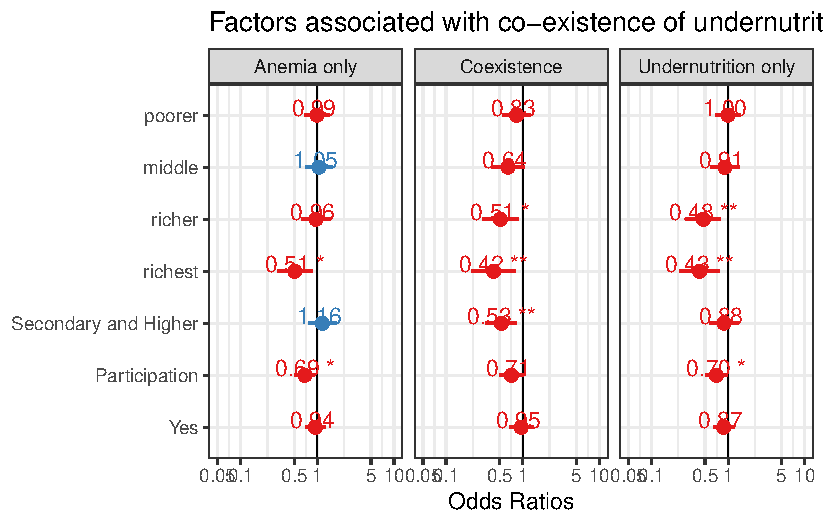
\includegraphics[width=0.85\linewidth,height=\textheight,keepaspectratio]{Section2/Categorical data analysis/Categorical_data_analysis2_files/figure-pdf/unnamed-chunk-26-1.pdf}
\end{center}

\section{Ordinal Logistic regression
Analysis}\label{ordinal-logistic-regression-analysis}

\subsection{Introduction}\label{introduction-7}

Ordinal logistic regression, extension of logistic regression, is a
statistical method used to analyze the relationship between an ordinal
dependent variable and one or more independent variables. An ordinal
variable is a categorical variable for which there is a clear ordering
of the category levels (a variable with ordered categories, such as
``low,'' ``medium,'' and ``high''). The explanatory variables may be
either continuous or categorical.

Estimating ordinal logistic regression models with statistical software
is not difficult, but the interpretation of the model output can be
cumbersome.It can be used to model outcomes such as satisfaction levels
or grades. The goal is to predict the probability of an observation
belonging to a certain category or a higher category, based on the
values of the independent variables

\subsection{Assumptions}\label{assumptions-2}

There are five assumptions that when violated may result in invalid
output. The five assumptions are:

\begin{enumerate}
\def\labelenumi{\arabic{enumi}.}
\tightlist
\item
  The dependent variable is measured on an ordinal level.
\item
  One or more of the independent variables are either continuous,
  categorical or ordinal.
\item
  Independence of observations and the dependent variable should be
  mutually exclusive.
\item
  No multi-collinearity
\item
  Proportional Odds : a major assumption of ordinal logistic regression
  is the assumption of proportional odds: the effect of an independent
  variable is constant for each increase in the level of the response.
  Hence the output of an ordinal logistic regression will contain an
  intercept for each level of the response except one, and a single
  slope for each explanatory variable.
\end{enumerate}

\subsection{Advantages and Disadvantages of Ordinal logistic
regression}\label{advantages-and-disadvantages-of-ordinal-logistic-regression}

\subsubsection{Advantages}\label{advantages-7}

\begin{itemize}
\item
  It handles ordered outcomes and retains the information of ordered
  outcome variable
\item
  It results in fewer parameters compared to multinomial logistic
  regression
\item
  It produces interpretable coefficients.
\end{itemize}

\subsubsection{Disadvantages}\label{disadvantages-7}

\begin{itemize}
\item
  It can only be used if it meets the proportional odds assumption
\item
  Not available in common libraries
\end{itemize}

Let's explore data to apply ordinal logistic regression analysis.

\subsection{Dataset, variables,
libraries}\label{dataset-variables-libraries}

\textbf{Dataset:} We have a subset of mental health data from NDHS 2022.

\textbf{Outcome variable:} \texttt{PHQ9\_Score} is the outcome variable.
We will convert it to a categorical variable named \texttt{depression}.
The categories of depression are Normal, Mild, Moderate, and Moderately
severe to severe. We will convert it to an ordinal variable.

\textbf{Independent variables:} In the following example we will take
four variables: \texttt{Age,\ Religion,\ Wealth,\ and\ Location.}

\textbf{Libraries:} We will use \texttt{tidyverse} (for data
manipulation), \texttt{gsheet} (to import the dataset), \texttt{MASS}
(to fit the ordinal logistic regression model), and \texttt{brant} (to
test the proportional odds assumption) packages.

\subsubsection{Load libraries and import
dataset}\label{load-libraries-and-import-dataset}

\begin{Shaded}
\begin{Highlighting}[]
\CommentTok{\# load library}
\FunctionTok{library}\NormalTok{(tidyverse) }\CommentTok{\# for data manipulation}
\FunctionTok{library}\NormalTok{(gsheet) }\CommentTok{\# to pull data from google sheet}
\FunctionTok{library}\NormalTok{(MASS) }\CommentTok{\# to use functions for ordinal regression}
\FunctionTok{library}\NormalTok{(brant) }\CommentTok{\# to test proportional odds assumption}

\CommentTok{\# import dataset}
\NormalTok{data}\OtherTok{\textless{}{-}}\NormalTok{gsheet}\SpecialCharTok{::}\FunctionTok{gsheet2tbl}\NormalTok{(}\StringTok{\textquotesingle{}https://docs.google.com/spreadsheets/d/1Sdp2kz0BD5x3nXTk8KlK6LtVy1MWnb\_hcWuo67mrWgs\textquotesingle{}}\NormalTok{)}

\FunctionTok{glimpse}\NormalTok{(data)}
\end{Highlighting}
\end{Shaded}

\begin{verbatim}
#> Rows: 12,353
#> Columns: 25
#> $ mcaseid              <chr> "1   1  1", "1   8  3", "1   8  6", "1   8  7", "~
#> $ Cluster              <dbl> 1, 1, 1, 1, 1, 1, 1, 1, 1, 1, 1, 2, 2, 2, 2, 2, 2~
#> $ Household            <dbl> 1, 8, 8, 8, 11, 11, 14, 14, 33, 39, 45, 7, 7, 9, ~
#> $ Line_number          <dbl> 1, 3, 6, 7, 3, 6, 1, 3, 1, 5, 1, 1, 3, 1, 1, 3, 1~
#> $ Sampling_weight      <dbl> 0.871652, 0.871652, 0.871652, 0.871652, 0.871652,~
#> $ Age                  <dbl> 31, 30, 21, 16, 29, 28, 49, 20, 34, 18, 35, 46, 1~
#> $ Sex                  <chr> "Male", "Male", "Male", "Male", "Male", "Male", "~
#> $ Ethnicity            <chr> "Janajati", "Brahmin_chhetri", "Brahmin_chhetri",~
#> $ Religion             <chr> "Hindu", "Hindu", "Hindu", "Hindu", "Hindu", "Hin~
#> $ marital_status       <dbl> 2, 2, 1, 1, 2, 2, 2, 1, 2, 1, 2, 2, 1, 2, 2, 1, 1~
#> $ Education            <dbl> 1, 1, 1, 1, 2, 1, 1, 1, 1, 2, 1, 1, 2, 3, 2, 1, 1~
#> $ occupation           <chr> "Agriculture", "Agriculture", "Agriculture", "Agr~
#> $ Location             <dbl> 1, 1, 1, 1, 1, 1, 1, 1, 1, 1, 1, 1, 1, 1, 1, 1, 1~
#> $ Ecologicalbelt       <chr> "mountain", "mountain", "mountain", "mountain", "~
#> $ Province             <chr> "koshi", "koshi", "koshi", "koshi", "koshi", "kos~
#> $ District             <chr> "taplejung", "taplejung", "taplejung", "taplejung~
#> $ Wealth               <chr> "poorest", "poorest", "poorest", "poorest", "poor~
#> $ Health_insurance     <dbl> 0, 0, 0, 0, 0, 0, 0, 0, 0, 0, 0, 0, 0, 0, 0, 0, 0~
#> $ current_alcohol      <chr> "some drink in past month", "some drink in past m~
#> $ current_smoke        <chr> "Do not smoke", "every day", "Do not smoke", "eve~
#> $ Self_reported_health <chr> "moderate", "good", "good", "good", "moderate", "~
#> $ disability           <dbl> 0, 0, 0, 0, 0, 0, 1, 0, 0, 0, 0, 1, 0, 1, 1, 0, 0~
#> $ Food_insecurity      <chr> "no", "yes", "yes", "yes", "no", "no", "no", "no"~
#> $ PHQ9_Score           <dbl> 0, 3, 0, 1, 1, 4, 0, 3, 0, 1, 0, 1, 0, 0, 3, 7, 0~
#> $ GAD_Score            <dbl> 0, 10, 0, 3, 3, 12, 4, 2, 1, 4, 1, 1, 1, 0, 1, 12~
\end{verbatim}

\subsubsection{Dataset preparation}\label{dataset-preparation}

\begin{Shaded}
\begin{Highlighting}[]
\CommentTok{\# Create categorical outcome variable depression}
\NormalTok{data}\OtherTok{\textless{}{-}}\NormalTok{data }\SpecialCharTok{|\textgreater{}}
  \FunctionTok{mutate}\NormalTok{(}\AttributeTok{depression=}\FunctionTok{case\_when}\NormalTok{(PHQ9\_Score}\SpecialCharTok{\textless{}=}\DecValTok{4}\SpecialCharTok{\textasciitilde{}}\DecValTok{0}\NormalTok{,}
\NormalTok{                          PHQ9\_Score}\SpecialCharTok{\textgreater{}}\DecValTok{4} \SpecialCharTok{\&}\NormalTok{ PHQ9\_Score}\SpecialCharTok{\textless{}}\DecValTok{10}\SpecialCharTok{\textasciitilde{}}\DecValTok{1}\NormalTok{,}
\NormalTok{                        PHQ9\_Score}\SpecialCharTok{\textgreater{}=}\DecValTok{10} \SpecialCharTok{\&}\NormalTok{ PHQ9\_Score}\SpecialCharTok{\textless{}}\DecValTok{15}\SpecialCharTok{\textasciitilde{}}\DecValTok{2}\NormalTok{,}
\NormalTok{                        PHQ9\_Score}\SpecialCharTok{\textgreater{}=}\DecValTok{15} \SpecialCharTok{\&}\NormalTok{ PHQ9\_Score}\SpecialCharTok{\textless{}}\DecValTok{28}\SpecialCharTok{\textasciitilde{}}\DecValTok{3}\NormalTok{))}

\CommentTok{\# converting depression variable to ordinal variable}
\NormalTok{data}\SpecialCharTok{$}\NormalTok{depression}\OtherTok{\textless{}{-}}\FunctionTok{factor}\NormalTok{(data}\SpecialCharTok{$}\NormalTok{depression, }\AttributeTok{levels =} \FunctionTok{c}\NormalTok{(}\DecValTok{0}\SpecialCharTok{:}\DecValTok{3}\NormalTok{), }\AttributeTok{labels=}\FunctionTok{c}\NormalTok{(}\StringTok{"Normal"}\NormalTok{, }\StringTok{"Mild"}\NormalTok{,}\StringTok{"Moderate"}\NormalTok{,}\StringTok{"Moderately severe to severe"}\NormalTok{), }\AttributeTok{ordered =}\NormalTok{T)}
\end{Highlighting}
\end{Shaded}

\subsubsection{Ordinal logistic regression
model}\label{ordinal-logistic-regression-model}

The proportional odds model (cumulative logit model) is the most widely
used ordinal logistic regression model. If the outcome variable M has k
categories (M=0, 1, 2, 3, \ldots, k), there are k-1 ways to dichotomize
the outcome variable. The odds of M\textgreater=k is :

\[ Odds (M \geq k) = \frac{P(M \geq k)}{1-P(M \geq k)} = \frac{P(M \geq k)}{P(M < k)} \]
where k =1, 2, 3,\ldots{} k-1

Under the proportional odds assumption, the odds ratio that compares
categories \textgreater=1 to \textless1 is the same as the odds ratio
that compares between \textgreater=2 to \textless2 or \textgreater=3 to
\textless3. This assumption results in only one coefficient for a
variable but k-1 intercepts.

The general regression model for ordinal logistic regression is as
follow:

\[ ln(\frac{P(M \geq k)} {P(M < k)}) = \alpha_k + \beta_1 X_1 +\beta_2X_2 +\beta_3X_3 \]
where k =1, 2, 3,\ldots{} k-1

\subsubsection{Ordinal logistic regression model
preparation}\label{ordinal-logistic-regression-model-preparation}

In a study to determine the association of depression (Normal/ mild/
moderate/ severe) with age (in years), religion (Hindu/ Non-Hindu),
wealth quintile (richest/ richer/ middle/ poorer/ poorest), and location
(rural/ urban), Lets create a theoretical model

\[ ln(\frac{P(Depression \geq k)} {P(Depression < k)}) = \alpha_k + \beta_1 Age +\beta_2Religion +\beta_3Wealth + \beta_4Location \]

The model in R can be created using \texttt{polr} function from the
\texttt{MASS} package as shown below:

\begin{Shaded}
\begin{Highlighting}[]
\CommentTok{\# Lets fit proportional odds logistic regression model}
\NormalTok{model1 }\OtherTok{\textless{}{-}} \FunctionTok{polr}\NormalTok{(depression }\SpecialCharTok{\textasciitilde{}}\NormalTok{ Age}\SpecialCharTok{+}\NormalTok{Religion}\SpecialCharTok{+}\NormalTok{Wealth}\SpecialCharTok{+}\NormalTok{Location, }\AttributeTok{data =}\NormalTok{ data, }\AttributeTok{Hess =}\NormalTok{ T)}

\CommentTok{\# See summary of the model}
\FunctionTok{summary}\NormalTok{(model1)}
\end{Highlighting}
\end{Shaded}

\begin{verbatim}
#> Call:
#> polr(formula = depression ~ Age + Religion + Wealth + Location, 
#>     data = data, Hess = T)
#> 
#> Coefficients:
#>                       Value Std. Error t value
#> Age                0.007322   0.002354  3.1110
#> ReligionNon_hindu  0.037160   0.064460  0.5765
#> Wealthpoorer       0.197368   0.073981  2.6678
#> Wealthpoorest      0.276796   0.070131  3.9469
#> Wealthricher      -0.129918   0.078599 -1.6529
#> Wealthrichest     -0.289871   0.089293 -3.2463
#> Location           0.075687   0.050717  1.4923
#> 
#> Intercepts:
#>                                      Value   Std. Error t value
#> Normal|Mild                           1.9432  0.1207    16.1061
#> Mild|Moderate                         3.5078  0.1267    27.6916
#> Moderate|Moderately severe to severe  4.9024  0.1467    33.4091
#> 
#> Residual Deviance: 14424.57 
#> AIC: 14444.57
\end{verbatim}

\subsubsection{Calculate p-value of ordinal logistic
regression}\label{calculate-p-value-of-ordinal-logistic-regression}

In order to determine p-value for ordinal logistic regression, we can
use the following code:

\begin{Shaded}
\begin{Highlighting}[]
\CommentTok{\# Generate coefficient table}
\NormalTok{coeff\_tab}\OtherTok{\textless{}{-}}\FunctionTok{round}\NormalTok{(}\FunctionTok{coef}\NormalTok{(}\FunctionTok{summary}\NormalTok{(model1)),}\DecValTok{3}\NormalTok{)}
\CommentTok{\# As the p{-}value is missing, let\textquotesingle{}s calculate the p{-}value table}
\NormalTok{p }\OtherTok{\textless{}{-}} \FunctionTok{pnorm}\NormalTok{(}\FunctionTok{abs}\NormalTok{(coeff\_tab[, }\StringTok{"t value"}\NormalTok{]), }\AttributeTok{lower.tail =}\NormalTok{ F) }\SpecialCharTok{*} \DecValTok{2}

\CommentTok{\# combine tables of coefficient and p{-}values }
\FunctionTok{cbind}\NormalTok{(coeff\_tab, }\StringTok{"p value"} \OtherTok{=} \FunctionTok{round}\NormalTok{(p, }\DecValTok{3}\NormalTok{))}
\end{Highlighting}
\end{Shaded}

\begin{verbatim}
#>                                       Value Std. Error t value p value
#> Age                                   0.007      0.002   3.111   0.002
#> ReligionNon_hindu                     0.037      0.064   0.576   0.565
#> Wealthpoorer                          0.197      0.074   2.668   0.008
#> Wealthpoorest                         0.277      0.070   3.947   0.000
#> Wealthricher                         -0.130      0.079  -1.653   0.098
#> Wealthrichest                        -0.290      0.089  -3.246   0.001
#> Location                              0.076      0.051   1.492   0.136
#> Normal|Mild                           1.943      0.121  16.106   0.000
#> Mild|Moderate                         3.508      0.127  27.692   0.000
#> Moderate|Moderately severe to severe  4.902      0.147  33.409   0.000
\end{verbatim}

\subsubsection{Determine odds ratio and
95\%CI}\label{determine-odds-ratio-and-95ci}

To calculate the odds ratio and 95\% confidence interval around the odds
ratio, we can use confint function to generate 95\% confidence interval
around coefficients. The coefficients can be exponentiated to calculate
odds ratio as shown in the code below.

\begin{tcolorbox}[enhanced jigsaw, bottomrule=.15mm, breakable, opacityback=0, toptitle=1mm, titlerule=0mm, bottomtitle=1mm, colback=white, arc=.35mm, rightrule=.15mm, toprule=.15mm, leftrule=.75mm, title=\textcolor{quarto-callout-tip-color}{\faLightbulb}\hspace{0.5em}{Tip}, colbacktitle=quarto-callout-tip-color!10!white, colframe=quarto-callout-tip-color-frame, coltitle=black, left=2mm, opacitybacktitle=0.6]

If the model contains interaction term then you can't directly calculate
odds ratio by exponentiation.

\end{tcolorbox}

\begin{Shaded}
\begin{Highlighting}[]
\CommentTok{\# Calculation of confidence intervals}
\NormalTok{conf\_int }\OtherTok{\textless{}{-}} \FunctionTok{round}\NormalTok{(}\FunctionTok{confint}\NormalTok{(model1), }\DecValTok{2}\NormalTok{)}

\CommentTok{\# log odds coefficients}
\NormalTok{odds\_ratio }\OtherTok{\textless{}{-}} \FunctionTok{round}\NormalTok{(}\FunctionTok{coef}\NormalTok{(model1), }\DecValTok{2}\NormalTok{)}

\CommentTok{\# convert coefficients into odds ratio, combine with CIs}
\FunctionTok{cbind}\NormalTok{(}\FunctionTok{round}\NormalTok{(}\FunctionTok{exp}\NormalTok{(}\FunctionTok{cbind}\NormalTok{(}\AttributeTok{OR =}\NormalTok{ odds\_ratio, conf\_int)), }\DecValTok{2}\NormalTok{), }\StringTok{"p{-}value"}\OtherTok{=}\FunctionTok{round}\NormalTok{(p,}\DecValTok{3}\NormalTok{))}
\end{Highlighting}
\end{Shaded}

\begin{verbatim}
#>                     OR 2.5 % 97.5 % p-value
#> Age               1.01  1.00   1.01   0.002
#> ReligionNon_hindu 1.04  0.91   1.17   0.565
#> Wealthpoorer      1.22  1.05   1.40   0.008
#> Wealthpoorest     1.32  1.15   1.51   0.000
#> Wealthricher      0.88  0.76   1.02   0.098
#> Wealthrichest     0.75  0.63   0.89   0.001
#> Location          1.08  0.98   1.20   0.136
\end{verbatim}

\subsubsection{Checking proportional odds
assumption}\label{checking-proportional-odds-assumption}

The brant test was defined by Rollin Brant to test the parallel
regression assumption. Assessing proportionality in the proportional
odds model for ordinal logistic regression.

\begin{Shaded}
\begin{Highlighting}[]
\CommentTok{\# testing parallel regression assumption using Brant\textquotesingle{}s test}
\FunctionTok{brant}\NormalTok{(model1)}
\end{Highlighting}
\end{Shaded}

\begin{verbatim}
#> ---------------------------------------------------- 
#> Test for     X2  df  probability 
#> ---------------------------------------------------- 
#> Omnibus          12.3    14  0.58
#> Age          0.84    2   0.66
#> ReligionNon_hindu    0.22    2   0.9
#> Wealthpoorer     0.9 2   0.64
#> Wealthpoorest        0.62    2   0.73
#> Wealthricher     0.78    2   0.68
#> Wealthrichest        3.29    2   0.19
#> Location     0.36    2   0.84
#> ---------------------------------------------------- 
#> 
#> H0: Parallel Regression Assumption holds
\end{verbatim}

Above is the Brant Test result for this dataset. We conclude that the
parallel assumption holds since the probability (p-values) for all
variables are greater than alpha=0.05. The output also contains an
Omnibus variable, which stands for the whole model, and it is still
greater than 0.05. Therefore the proportional odds assumption is not
violated and the model is a valid model for this dataset.

\subsubsection{Checking
multi-collinearity}\label{checking-multi-collinearity}

\begin{Shaded}
\begin{Highlighting}[]
\NormalTok{model2}\OtherTok{\textless{}{-}} \FunctionTok{glm}\NormalTok{(PHQ9\_Score}\SpecialCharTok{\textasciitilde{}}\NormalTok{ Age}\SpecialCharTok{+}\NormalTok{Religion}\SpecialCharTok{+}\NormalTok{Wealth}\SpecialCharTok{+}\NormalTok{Location, }\AttributeTok{data =}\NormalTok{ data, }\AttributeTok{family =} \FunctionTok{gaussian}\NormalTok{(}\AttributeTok{link=}\StringTok{"identity"}\NormalTok{))}

\NormalTok{performance}\SpecialCharTok{::}\FunctionTok{check\_collinearity}\NormalTok{(model2)}
\end{Highlighting}
\end{Shaded}

\begin{verbatim}
#> # Check for Multicollinearity
#> 
#> Low Correlation
#> 
#>      Term  VIF   VIF 95% CI adj. VIF Tolerance Tolerance 95% CI
#>       Age 1.00 [1.00, 1.91]     1.00      1.00     [0.52, 1.00]
#>  Religion 1.01 [1.00, 1.17]     1.00      0.99     [0.85, 1.00]
#>    Wealth 1.16 [1.14, 1.18]     1.08      0.86     [0.85, 0.88]
#>  Location 1.16 [1.14, 1.18]     1.08      0.86     [0.84, 0.88]
\end{verbatim}

Multicollinearity occurs when two or more predictors in the model are
correlated and provide redundant information about the response.
Multicollinearity was measured by variance inflation factors (VIF) and
tolerance. If VIF value exceeding 4.0, or by tol- erance less than 0.2
then there is a problem with multicollinearity (Hair et al., 2010). Here
in our model the VIF is lower than 4 so there is no presence of multi-co
linearity.

\subsubsection{Interpretation of odds
ratio}\label{interpretation-of-odds-ratio}

\begin{Shaded}
\begin{Highlighting}[]
\FunctionTok{cbind}\NormalTok{(}\FunctionTok{round}\NormalTok{(}\FunctionTok{exp}\NormalTok{(}\FunctionTok{cbind}\NormalTok{(}\AttributeTok{OR =}\NormalTok{ odds\_ratio, conf\_int)), }\DecValTok{2}\NormalTok{), }\StringTok{"p{-}value"}\OtherTok{=}\FunctionTok{round}\NormalTok{(p,}\DecValTok{3}\NormalTok{))}
\end{Highlighting}
\end{Shaded}

\begin{verbatim}
#>                     OR 2.5 % 97.5 % p-value
#> Age               1.01  1.00   1.01   0.002
#> ReligionNon_hindu 1.04  0.91   1.17   0.565
#> Wealthpoorer      1.22  1.05   1.40   0.008
#> Wealthpoorest     1.32  1.15   1.51   0.000
#> Wealthricher      0.88  0.76   1.02   0.098
#> Wealthrichest     0.75  0.63   0.89   0.001
#> Location          1.08  0.98   1.20   0.136
\end{verbatim}

The odds of having a higher level of depression compared to a lower
level is 1.01 (95\% CI: 1.00 to 1.01) times higher for each additional
year of age, after adjusting for religion, wealth, and place of
residence. Compared to the middle wealth quintile, the odds of having a
higher level of depression are 25\% lower among participants from the
richest wealth quintile (OR: 0.75; 95\% CI: 0.63 to 0.89) and 32\%
higher among participants from the poorest wealth quintile (OR: 1.32;
95\% CI: 1.15 to 1.51), after adjusting for age, religion, and place of
residence.

\chapter{Summary}\label{summary-7}

This chapter covered logistic regression and its major extensions for
analyzing categorical outcomes. Standard binary logistic regression
(univariate, multivariable, and with interaction terms) is appropriate
for a binary outcome with independent observations. When the outcome is
binary but the data are sparse or perfectly separated, exact logistic
regression or Firth's penalized logistic regression provide more
reliable estimates than standard maximum likelihood. When observations
are clustered or repeated within subjects, generalized estimating
equations (GEE) extend the logistic model to yield valid,
population-averaged inference. When the outcome variable has more than
two unordered categories, multinomial logistic regression is used, while
ordinal logistic regression is preferred when the outcome categories
have a natural order, provided the proportional odds assumption holds.
Selecting among these methods depends primarily on the structure of the
outcome variable (binary, nominal, or ordinal), the independence or
clustering of observations, and the sample size and event frequency.

\chapter{Count Data analysis}\label{count-data-analysis}

\section{Count data}\label{count-data}

The data consisting of non-negative integers values which is the count
of occurrence of events. Due to the discrete nature, the count data
can't be treated as continuous variables. The categorical analysis
methods are also not appropriate. The examples of count data are:

a) Number of risk factors of NCDs present in a person

b) Number of people visiting doctor's office per month

\section{Poisson Distribution}\label{poisson-distribution-1}

It is the distribution if we want to calculate the probabilities of the
number of ocurences of some phenomenon in some space or time interval,
often measured as the rate (average given the measired space).

\[
f(x)= \frac{e^{-\lambda}*\lambda^x}{x!}, x=1,2,...
\]

\[
E(x)=Var(x) = lambda
\]

\(\lambda\) (rate) is the average number of some success in sometime
span.

\section{Poisson Regression}\label{poisson-regression}

Poisson regression is particularly useful for:

\begin{itemize}
\tightlist
\item
  Modeling the count of events occurring within a fixed period or space.
\item
  Predicting counts based on predictor variables.
\end{itemize}

The general form of the Poisson regression model is:

\[
\log(\lambda_i) = \beta_0 + \beta_1 X_1 + \beta_2 X_2 + \ldots + \beta_n X_n
\]

\begin{center}\rule{0.5\linewidth}{0.5pt}\end{center}

\subsection{Assumptions of Poisson
Regression}\label{assumptions-of-poisson-regression}

\begin{enumerate}
\def\labelenumi{\arabic{enumi}.}
\item
  \textbf{Poisson Distribution}: The response variable ( Y\_i ) follows
  a Poisson distribution. \[
  Y_i \sim \text{Poisson}(\lambda_i)
  \]
\item
  \textbf{Log Link Function}: The logarithm of the mean ( \lambda\_i )
  is linearly related to the predictors. \[
  \log(\lambda_i) = X\beta
  \]
\item
  \textbf{Equality of Mean and Variance}: The mean and variance of the
  response variable are equal. \[
  E(Y_i) = Var(Y_i) = \lambda_i
  \]
\item
  \textbf{Independence}: Observations are independent of each other.
\item
  \textbf{No Multi-collinearity}: Predictor variables should not exhibit
  high collinearity.
\end{enumerate}

\begin{center}\rule{0.5\linewidth}{0.5pt}\end{center}

\section{Worked Example: Poisson Regression in
R}\label{worked-example-poisson-regression-in-r}

We use the same simulated dataset as the rest of this chapter
(\texttt{ed\_visits.csv}, \(n=400\)): a cohort of adult patients
followed for one year, with outcome \texttt{ed\_visits} (number of
Emergency Department visits) and predictors \texttt{age},
\texttt{smoker}, \texttt{chronic} (number of chronic conditions), and
\texttt{insured}.

\begin{Shaded}
\begin{Highlighting}[]
\NormalTok{dat }\OtherTok{\textless{}{-}} \FunctionTok{read.csv}\NormalTok{(}\StringTok{"D:/Epi Biostat with R/Biostat\_with\_R/Section2/Count data analysis/ed\_visits.csv"}\NormalTok{)}
\NormalTok{dat}\SpecialCharTok{$}\NormalTok{age\_c }\OtherTok{\textless{}{-}}\NormalTok{ (dat}\SpecialCharTok{$}\NormalTok{age }\SpecialCharTok{{-}} \DecValTok{50}\NormalTok{) }\SpecialCharTok{/} \DecValTok{10}   \CommentTok{\# age centered at 50, scaled per decade}
\FunctionTok{head}\NormalTok{(dat)}
\end{Highlighting}
\end{Shaded}

\begin{verbatim}
#>   age smoker chronic insured ed_visits age_c
#> 1  30      0       2       1         0  -2.0
#> 2  61      0       2       1         1   1.1
#> 3  49      0       2       0         0  -0.1
#> 4  43      0       1       1         0  -0.7
#> 5  42      0       0       1         0  -0.8
#> 6  71      0       1       1         0   2.1
\end{verbatim}

\subsection{Fit the model}\label{fit-the-model}

\begin{Shaded}
\begin{Highlighting}[]
\NormalTok{m\_pois }\OtherTok{\textless{}{-}} \FunctionTok{glm}\NormalTok{(ed\_visits }\SpecialCharTok{\textasciitilde{}}\NormalTok{ age\_c }\SpecialCharTok{+}\NormalTok{ smoker }\SpecialCharTok{+}\NormalTok{ chronic }\SpecialCharTok{+}\NormalTok{ insured,}
              \AttributeTok{family =} \FunctionTok{poisson}\NormalTok{(}\AttributeTok{link =} \StringTok{"log"}\NormalTok{), }\AttributeTok{data =}\NormalTok{ dat)}
\FunctionTok{summary}\NormalTok{(m\_pois)}
\end{Highlighting}
\end{Shaded}

\begin{verbatim}
#> 
#> Call:
#> glm(formula = ed_visits ~ age_c + smoker + chronic + insured, 
#>     family = poisson(link = "log"), data = dat)
#> 
#> Coefficients:
#>             Estimate Std. Error z value Pr(>|z|)    
#> (Intercept) -0.99973    0.11273  -8.868  < 2e-16 ***
#> age_c        0.64145    0.02747  23.348  < 2e-16 ***
#> smoker       0.10107    0.07400   1.366 0.171991    
#> chronic      0.43979    0.03138  14.014  < 2e-16 ***
#> insured      0.29965    0.08769   3.417 0.000633 ***
#> ---
#> Signif. codes:  0 '***' 0.001 '**' 0.01 '*' 0.05 '.' 0.1 ' ' 1
#> 
#> (Dispersion parameter for poisson family taken to be 1)
#> 
#>     Null deviance: 2086.9  on 399  degrees of freedom
#> Residual deviance: 1197.0  on 395  degrees of freedom
#> AIC: 1653.6
#> 
#> Number of Fisher Scoring iterations: 6
\end{verbatim}

\subsection{Interpreting coefficients as Incidence Rate Ratios
(IRRs)}\label{interpreting-coefficients-as-incidence-rate-ratios-irrs}

Because the log link is used, exponentiating the coefficients converts
them from the log scale to \textbf{incidence rate ratios} --- the
multiplicative change in the expected count per one-unit increase in the
predictor.

\begin{Shaded}
\begin{Highlighting}[]
\FunctionTok{exp}\NormalTok{(}\FunctionTok{cbind}\NormalTok{(}\AttributeTok{IRR =} \FunctionTok{coef}\NormalTok{(m\_pois), }\FunctionTok{confint}\NormalTok{(m\_pois)))}
\end{Highlighting}
\end{Shaded}

\begin{verbatim}
#>                   IRR     2.5 %    97.5 %
#> (Intercept) 0.3679788 0.2939149 0.4572799
#> age_c       1.8992313 1.8010611 2.0059258
#> smoker      1.1063528 0.9563549 1.2783456
#> chronic     1.5523778 1.4596413 1.6507482
#> insured     1.3493914 1.1392668 1.6069800
\end{verbatim}

For example, an IRR of 1.68 for \texttt{chronic} means each additional
chronic condition is associated with a 68\% increase in expected ED
visits, holding other predictors constant.

\subsection{Predicted counts}\label{predicted-counts}

\begin{Shaded}
\begin{Highlighting}[]
\NormalTok{dat}\SpecialCharTok{$}\NormalTok{pred\_visits }\OtherTok{\textless{}{-}} \FunctionTok{predict}\NormalTok{(m\_pois, }\AttributeTok{type =} \StringTok{"response"}\NormalTok{)}
\FunctionTok{head}\NormalTok{(dat[, }\FunctionTok{c}\NormalTok{(}\StringTok{"age"}\NormalTok{, }\StringTok{"smoker"}\NormalTok{, }\StringTok{"chronic"}\NormalTok{, }\StringTok{"insured"}\NormalTok{, }\StringTok{"ed\_visits"}\NormalTok{, }\StringTok{"pred\_visits"}\NormalTok{)])}
\end{Highlighting}
\end{Shaded}

\begin{verbatim}
#>   age smoker chronic insured ed_visits pred_visits
#> 1  30      0       2       1         0   0.3317416
#> 2  61      0       2       1         1   2.4232111
#> 3  49      0       2       0         0   0.8316870
#> 4  43      0       1       1         0   0.4919871
#> 5  42      0       0       1         0   0.2972340
#> 6  71      0       1       1         0   2.9646381
\end{verbatim}

\subsection{Modeling rates with an
offset}\label{modeling-rates-with-an-offset}

When counts are observed over varying amounts of time or exposure (e.g.,
person-years of follow-up), an \textbf{offset} is used so the model
estimates a \emph{rate} rather than a raw count. If \texttt{dat\$time}
held each patient's follow-up time, the model would be:

\begin{Shaded}
\begin{Highlighting}[]
\NormalTok{m\_rate }\OtherTok{\textless{}{-}} \FunctionTok{glm}\NormalTok{(ed\_visits }\SpecialCharTok{\textasciitilde{}}\NormalTok{ age\_c }\SpecialCharTok{+}\NormalTok{ smoker }\SpecialCharTok{+}\NormalTok{ chronic }\SpecialCharTok{+}\NormalTok{ insured,}
              \AttributeTok{family =} \FunctionTok{poisson}\NormalTok{(}\AttributeTok{link =} \StringTok{"log"}\NormalTok{),}
              \AttributeTok{offset =} \FunctionTok{log}\NormalTok{(time), }\AttributeTok{data =}\NormalTok{ dat)}
\end{Highlighting}
\end{Shaded}

The offset enters the model with a fixed coefficient of 1, so
\texttt{log(lambda\_i\ /\ time\_i)} is modeled instead of
\texttt{log(lambda\_i)} --- the fitted coefficients are then interpreted
as rate ratios per unit time.

\subsection{Goodness of fit}\label{goodness-of-fit}

\begin{Shaded}
\begin{Highlighting}[]
\DecValTok{1} \SpecialCharTok{{-}} \FunctionTok{pchisq}\NormalTok{(}\FunctionTok{deviance}\NormalTok{(m\_pois), }\AttributeTok{df =}\NormalTok{ m\_pois}\SpecialCharTok{$}\NormalTok{df.residual)}
\end{Highlighting}
\end{Shaded}

\begin{verbatim}
#> [1] 0
\end{verbatim}

A small p-value here suggests the model does not fit well --- this is
the first diagnostic that motivates checking for overdispersion and
excess zeros, covered next.

\section{Overdispersion and Zero-Inflated Count
Models}\label{overdispersion-and-zero-inflated-count-models}

\subsection{Why Poisson Regression Is Often Not
Enough}\label{why-poisson-regression-is-often-not-enough}

Poisson regression, which rests on a strict assumption: \textbf{the mean
and the variance of the count are equal}, \(E(Y_i)=Var(Y_i)=\lambda_i\).
Real health-count data almost never behave this politely. Two problems
show up constantly in clinical and public-health data:

\begin{enumerate}
\def\labelenumi{\arabic{enumi}.}
\tightlist
\item
  \textbf{Overdispersion} --- the observed variance is \emph{larger}
  than the mean (sometimes far larger), because of unmeasured
  heterogeneity between patients, clustering of events within a person,
  or contagion-type processes (one hospitalization increases the risk of
  another).
\item
  \textbf{Excess zeros} --- the data contain more zero counts than a
  Poisson (or even a Negative Binomial) distribution would predict,
  because some individuals are structurally incapable of generating a
  positive count (e.g., a never-smoker cannot have a smoking-related
  complication count above zero) while others simply happened to have a
  zero during the observation window.
\end{enumerate}

Ignoring either problem does not just produce a ``slightly wrong'' model
--- it produces \textbf{standard errors that are too small}, which
inflates Type-I error and makes non-significant predictors look
significant. This chapter builds, step by step, the toolbox used to
diagnose and correct these problems:

\begin{itemize}
\tightlist
\item
  \textbf{Negative Binomial (NB) regression} --- corrects
  overdispersion.
\item
  \textbf{Zero-Inflated Poisson (ZIP) regression} --- corrects excess
  zeros when counts are otherwise equidispersed.
\item
  \textbf{Zero-Inflated Negative Binomial (ZINB) regression} ---
  corrects excess zeros \emph{and} overdispersion simultaneously.
\item
  A short note on \textbf{Hurdle models}, a close relative of the
  zero-inflated family.
\end{itemize}

Every model below is fit on the same worked health example so the
numbers can be compared directly.

\begin{center}\rule{0.5\linewidth}{0.5pt}\end{center}

\subsection{Worked Example: Emergency Department (ED)
Visits}\label{worked-example-emergency-department-ed-visits}

Imagine a cohort of 400 adult patients followed for one year, and we
count each patient's number of \textbf{Emergency Department visits}.
Predictors collected at baseline are:

a) \texttt{age} --- age in years

b) \texttt{smoker} --- current smoker (1) vs.~non-smoker (0)

c) \texttt{chronic} --- number of chronic conditions (0--4): diabetes,
hypertension, COPD, heart disease

d) \texttt{insured} --- has health insurance (1) vs.~does not (0)

This is a realistic setting for \textbf{two separate zero-generating
mechanisms}: some patients are simply not ``at risk'' of an ED visit in
a given year (healthy, well-controlled, good access to primary care ---
a \emph{structural} zero), while others are at risk but simply happened
not to visit during the window (a \emph{sampling} zero, drawn from a
Poisson/NB process). This is exactly the situation zero-inflated models
were built for.

The simulated dataset (\texttt{ed\_visits.csv}, \(n=400\)) used
throughout this chapter is saved alongside this file so every result
below is fully reproducible.

\subsection{Rcode}\label{rcode}

\begin{Shaded}
\begin{Highlighting}[]
\FunctionTok{library}\NormalTok{(MASS)     }\CommentTok{\# glm.nb()}
\FunctionTok{library}\NormalTok{(pscl)      }\CommentTok{\# zeroinfl(), odTest(), vuong()}
\FunctionTok{library}\NormalTok{(AER)        }\CommentTok{\# dispersiontest()}

\NormalTok{dat }\OtherTok{\textless{}{-}} \FunctionTok{read.csv}\NormalTok{(}\StringTok{"ed\_visits.csv"}\NormalTok{)}
\NormalTok{dat}\SpecialCharTok{$}\NormalTok{age\_c }\OtherTok{\textless{}{-}}\NormalTok{ (dat}\SpecialCharTok{$}\NormalTok{age }\SpecialCharTok{{-}} \DecValTok{50}\NormalTok{) }\SpecialCharTok{/} \DecValTok{10}   \CommentTok{\# age centered at 50, scaled per decade}
\FunctionTok{str}\NormalTok{(dat)}
\end{Highlighting}
\end{Shaded}

\begin{verbatim}
#> 'data.frame':    400 obs. of  6 variables:
#>  $ age      : int  30 61 49 43 42 71 79 30 62 38 ...
#>  $ smoker   : int  0 0 0 0 0 0 0 1 0 1 ...
#>  $ chronic  : int  2 2 2 1 0 1 2 2 3 4 ...
#>  $ insured  : int  1 1 0 1 1 1 1 0 1 1 ...
#>  $ ed_visits: int  0 1 0 0 0 0 6 2 2 0 ...
#>  $ age_c    : num  -2 1.1 -0.1 -0.7 -0.8 2.1 2.9 -2 1.2 -1.2 ...
\end{verbatim}

A quick look at the outcome already hints at trouble:

\begin{Shaded}
\begin{Highlighting}[]
\FunctionTok{mean}\NormalTok{(dat}\SpecialCharTok{$}\NormalTok{ed\_visits)}
\end{Highlighting}
\end{Shaded}

\begin{verbatim}
#> [1] 1.8975
\end{verbatim}

\begin{Shaded}
\begin{Highlighting}[]
\FunctionTok{var}\NormalTok{(dat}\SpecialCharTok{$}\NormalTok{ed\_visits)}
\end{Highlighting}
\end{Shaded}

\begin{verbatim}
#> [1] 14.18746
\end{verbatim}

\begin{Shaded}
\begin{Highlighting}[]
\FunctionTok{prop.table}\NormalTok{(}\FunctionTok{table}\NormalTok{(dat}\SpecialCharTok{$}\NormalTok{ed\_visits }\SpecialCharTok{==} \DecValTok{0}\NormalTok{))}
\end{Highlighting}
\end{Shaded}

\begin{verbatim}
#> 
#> FALSE  TRUE 
#>  0.34  0.66
\end{verbatim}

The mean number of visits is about \textbf{1.90}, but the variance is
about \textbf{14.2} --- roughly \textbf{7.5 times larger} than the mean.
Under a true Poisson process these should be equal. In addition,
\textbf{66\%} of patients have zero ED visits. Both signs point away
from a plain Poisson model, but we fit it first anyway, because the
diagnostics it produces are exactly what justify moving to the more
complex models.

\begin{center}\rule{0.5\linewidth}{0.5pt}\end{center}

\subsection{Fit Poisson Regression and Check the
Assumptions}\label{fit-poisson-regression-and-check-the-assumptions}

\begin{Shaded}
\begin{Highlighting}[]
\NormalTok{m\_pois }\OtherTok{\textless{}{-}} \FunctionTok{glm}\NormalTok{(ed\_visits }\SpecialCharTok{\textasciitilde{}}\NormalTok{ age\_c }\SpecialCharTok{+}\NormalTok{ smoker }\SpecialCharTok{+}\NormalTok{ chronic }\SpecialCharTok{+}\NormalTok{ insured,}
              \AttributeTok{family =} \FunctionTok{poisson}\NormalTok{(}\AttributeTok{link =} \StringTok{"log"}\NormalTok{), }\AttributeTok{data =}\NormalTok{ dat)}
\FunctionTok{summary}\NormalTok{(m\_pois)}
\end{Highlighting}
\end{Shaded}

\begin{verbatim}
#> 
#> Call:
#> glm(formula = ed_visits ~ age_c + smoker + chronic + insured, 
#>     family = poisson(link = "log"), data = dat)
#> 
#> Coefficients:
#>             Estimate Std. Error z value Pr(>|z|)    
#> (Intercept) -0.99973    0.11273  -8.868  < 2e-16 ***
#> age_c        0.64145    0.02747  23.348  < 2e-16 ***
#> smoker       0.10107    0.07400   1.366 0.171991    
#> chronic      0.43979    0.03138  14.014  < 2e-16 ***
#> insured      0.29965    0.08769   3.417 0.000633 ***
#> ---
#> Signif. codes:  0 '***' 0.001 '**' 0.01 '*' 0.05 '.' 0.1 ' ' 1
#> 
#> (Dispersion parameter for poisson family taken to be 1)
#> 
#>     Null deviance: 2086.9  on 399  degrees of freedom
#> Residual deviance: 1197.0  on 395  degrees of freedom
#> AIC: 1653.6
#> 
#> Number of Fisher Scoring iterations: 6
\end{verbatim}

\textbf{Formal overdispersion test} (Cameron \& Trivedi regression-based
test):

\begin{Shaded}
\begin{Highlighting}[]
\FunctionTok{dispersiontest}\NormalTok{(m\_pois)}
\end{Highlighting}
\end{Shaded}

\begin{verbatim}
#> 
#>  Overdispersion test
#> 
#> data:  m_pois
#> z = 4.7601, p-value = 9.674e-07
#> alternative hypothesis: true dispersion is greater than 1
#> sample estimates:
#> dispersion 
#>   4.063466
\end{verbatim}

\textbf{Comparing observed vs.~Poisson-predicted zeros:}

\begin{Shaded}
\begin{Highlighting}[]
\NormalTok{mu\_hat }\OtherTok{\textless{}{-}} \FunctionTok{fitted}\NormalTok{(m\_pois)}
\NormalTok{obs\_zero  }\OtherTok{\textless{}{-}} \FunctionTok{mean}\NormalTok{(dat}\SpecialCharTok{$}\NormalTok{ed\_visits }\SpecialCharTok{==} \DecValTok{0}\NormalTok{)}
\NormalTok{pred\_zero }\OtherTok{\textless{}{-}} \FunctionTok{mean}\NormalTok{(}\FunctionTok{exp}\NormalTok{(}\SpecialCharTok{{-}}\NormalTok{mu\_hat))}
\FunctionTok{c}\NormalTok{(}\AttributeTok{observed =}\NormalTok{ obs\_zero, }\AttributeTok{poisson\_predicted =}\NormalTok{ pred\_zero)}
\end{Highlighting}
\end{Shaded}

\begin{verbatim}
#>          observed poisson_predicted 
#>         0.6600000         0.4074593
\end{verbatim}

\subsection{Interpretation}\label{interpretation-27}

The dispersion statistic is about \textbf{4.1} (should be \(\approx 1\)
under a true Poisson model), and \texttt{dispersiontest()} rejects
equidispersion at \(p<0.001\). The model also badly under-predicts
zeros: Poisson expects only about \textbf{41\%} zero visits, but
\textbf{66\%} are observed in the data. Both diagnostics say the same
thing: \textbf{Poisson regression is not adequate here}, and any
p-values from \texttt{m\_pois} should not be trusted --- they are too
optimistic (SEs too small). This is the standard trigger for moving to
Negative Binomial regression.

\section{Negative Binomial
Regression}\label{negative-binomial-regression}

\subsection{The model}\label{the-model}

The Negative Binomial (NB2, the standard parameterization) extends
Poisson by adding a dispersion parameter \(\alpha>0\):

\[
Var(Y_i) = \mu_i + \alpha\,\mu_i^2
\]

When \(\alpha \to 0\), NB collapses back to Poisson (\(Var=\mu\)), which
is why Poisson is a special case of NB and the two can be compared with
a likelihood-ratio test. The mean structure is unchanged,
\(\log(\mu_i)=X_i\beta\), so the \textbf{interpretation of coefficients
is identical to Poisson} (incidence rate ratios, IRRs) --- only the
variance (and therefore the standard errors and p-values) is corrected.

\subsection{When to use Negative Binomial instead of
Poisson}\label{when-to-use-negative-binomial-instead-of-poisson}

\begin{itemize}
\tightlist
\item
  The Pearson/deviance dispersion statistic is noticeably \(>1\)
  (commonly used rule of thumb: \(>1.5\)--\(2\) deserves attention; here
  it is \(4.1\)).
\item
  \texttt{dispersiontest()} (or an equivalent LR/score test) rejects
  equidispersion.
\item
  Overdispersion is plausibly due to \textbf{unobserved heterogeneity}
  between subjects rather than a distinct ``always-zero'' subpopulation
  (if the zeros look structurally different from the rest, consider
  zero-inflated models first --- see below).
\item
  There is \textbf{no strong a-priori reason to model the zeros with a
  separate process} --- NB simply lets the whole distribution be more
  spread out, including allowing more zeros than Poisson.
\end{itemize}

\begin{Shaded}
\begin{Highlighting}[]
\NormalTok{m\_nb }\OtherTok{\textless{}{-}} \FunctionTok{glm.nb}\NormalTok{(ed\_visits }\SpecialCharTok{\textasciitilde{}}\NormalTok{ age\_c }\SpecialCharTok{+}\NormalTok{ smoker }\SpecialCharTok{+}\NormalTok{ chronic }\SpecialCharTok{+}\NormalTok{ insured, }\AttributeTok{data =}\NormalTok{ dat)}
\FunctionTok{summary}\NormalTok{(m\_nb)}
\end{Highlighting}
\end{Shaded}

\begin{verbatim}
#> 
#> Call:
#> glm.nb(formula = ed_visits ~ age_c + smoker + chronic + insured, 
#>     data = dat, init.theta = 0.3862060674, link = log)
#> 
#> Coefficients:
#>             Estimate Std. Error z value Pr(>|z|)    
#> (Intercept) -1.05631    0.23936  -4.413 1.02e-05 ***
#> age_c        0.65827    0.06023  10.929  < 2e-16 ***
#> smoker       0.08189    0.20615   0.397    0.691    
#> chronic      0.51981    0.08733   5.952 2.64e-09 ***
#> insured      0.19036    0.21971   0.866    0.386    
#> ---
#> Signif. codes:  0 '***' 0.001 '**' 0.01 '*' 0.05 '.' 0.1 ' ' 1
#> 
#> (Dispersion parameter for Negative Binomial(0.3862) family taken to be 1)
#> 
#>     Null deviance: 472.86  on 399  degrees of freedom
#> Residual deviance: 304.78  on 395  degrees of freedom
#> AIC: 1143.9
#> 
#> Number of Fisher Scoring iterations: 1
#> 
#> 
#>               Theta:  0.3862 
#>           Std. Err.:  0.0548 
#> 
#>  2 x log-likelihood:  -1131.8870
\end{verbatim}

Incidence rate ratios (IRRs) with 95\% CIs:

\begin{Shaded}
\begin{Highlighting}[]
\FunctionTok{exp}\NormalTok{(}\FunctionTok{cbind}\NormalTok{(}\AttributeTok{IRR =} \FunctionTok{coef}\NormalTok{(m\_nb), }\FunctionTok{confint}\NormalTok{(m\_nb)))}
\end{Highlighting}
\end{Shaded}

\begin{verbatim}
#>                   IRR     2.5 %    97.5 %
#> (Intercept) 0.3477372 0.2127285 0.5681924
#> age_c       1.9314550 1.7199622 2.1814970
#> smoker      1.0853375 0.7264347 1.6309138
#> chronic     1.6817129 1.4115011 2.0185060
#> insured     1.2096867 0.7747641 1.8643213
\end{verbatim}

\textbf{Formal test of whether NB is needed over Poisson}
(likelihood-ratio test on the boundary of \(\alpha=0\), implemented in
\texttt{pscl::odTest}):

\begin{Shaded}
\begin{Highlighting}[]
\FunctionTok{odTest}\NormalTok{(m\_nb)}
\end{Highlighting}
\end{Shaded}

\begin{verbatim}
#> Likelihood ratio test of H0: Poisson, as restricted NB model:
#> n.b., the distribution of the test-statistic under H0 is non-standard
#> e.g., see help(odTest) for details/references
#> 
#> Critical value of test statistic at the alpha= 0.05 level: 2.7055 
#> Chi-Square Test Statistic =  511.7369 p-value = < 2.2e-16
\end{verbatim}

\textbf{Zero-count check for NB:}

\begin{Shaded}
\begin{Highlighting}[]
\NormalTok{mu\_nb    }\OtherTok{\textless{}{-}} \FunctionTok{fitted}\NormalTok{(m\_nb)}
\NormalTok{theta\_nb }\OtherTok{\textless{}{-}}\NormalTok{ m\_nb}\SpecialCharTok{$}\NormalTok{theta}
\NormalTok{p\_nb0 }\OtherTok{\textless{}{-}} \FunctionTok{mean}\NormalTok{((theta\_nb }\SpecialCharTok{/}\NormalTok{ (theta\_nb }\SpecialCharTok{+}\NormalTok{ mu\_nb))}\SpecialCharTok{\^{}}\NormalTok{theta\_nb)}
\FunctionTok{c}\NormalTok{(}\AttributeTok{observed =}\NormalTok{ obs\_zero, }\AttributeTok{nb\_predicted =}\NormalTok{ p\_nb0)}
\end{Highlighting}
\end{Shaded}

\begin{verbatim}
#>     observed nb_predicted 
#>     0.660000     0.622975
\end{verbatim}

\subsection{Interpretation}\label{interpretation-28}

\texttt{odTest()} gives a large LR statistic with \(p<0.001\):
overdispersion is real, and NB is a significantly better fit than
Poisson (AIC drops from about \textbf{1654} to about \textbf{1144}). The
estimated dispersion parameter \(\hat\theta \approx 0.39\) (equivalently
\(\hat\alpha = 1/\theta \approx 2.6\)) is far from the Poisson limit of
\(\theta\to\infty\), confirming strong overdispersion.

Reading the IRRs: each additional chronic condition multiplies the
expected number of ED visits by about \(e^{0.52}\approx1.68\) (68\% more
visits per chronic condition, holding other variables fixed), and each
10-year increase in age multiplies expected visits by about
\(e^{0.66}\approx1.93\). Smoking status and insurance are no longer
significant once overdispersion is properly accounted for (their Poisson
p-values were artificially small).

The NB model also predicts the zero proportion much better than Poisson
(\textbf{62\%} vs.~the \textbf{66\%} observed) --- but not perfectly.
That residual gap is the signature of \textbf{excess zeros that NB alone
cannot fully explain}, which motivates the zero-inflated models next.

\section{Zero-Inflated Poisson (ZIP)
Regression}\label{zero-inflated-poisson-zip-regression}

\subsection{The model}\label{the-model-1}

ZIP treats the data as coming from a \textbf{two-component mixture}:

\begin{itemize}
\tightlist
\item
  With probability \(\pi_i\), the observation is a \textbf{``certain''
  (structural) zero} --- the patient is simply not in the at-risk
  population for this event.
\item
  With probability \(1-\pi_i\), the observation comes from a standard
  \textbf{Poisson} process with mean \(\mu_i\) (which can itself produce
  a zero by chance).
\end{itemize}

\[
P(Y_i = 0) = \pi_i + (1-\pi_i)e^{-\mu_i} \qquad\qquad P(Y_i = y) = (1-\pi_i)\,\frac{e^{-\mu_i}\mu_i^{y}}{y!},\ \ y=1,2,\dots
\]

Two linear predictors are estimated simultaneously:

\[
\log(\mu_i) = X_i\beta \quad \text{(count model — "how many events, if any risk exists")}
\]

\[
\text{logit}(\pi_i) = Z_i\gamma \quad \text{(zero-inflation model — "probability of being structurally not at risk")}
\]

\subsection{When to use ZIP}\label{when-to-use-zip}

\begin{itemize}
\tightlist
\item
  There is a \textbf{substantively meaningful subgroup that cannot
  experience the event at all} (e.g., patients with no disease exposure,
  no relevant risk factor, or excellent disease control), distinct from
  patients who are at risk but simply recorded a zero.
\item
  The proportion of zeros observed is clearly larger than a Poisson
  model predicts.
\item
  Among the ``at-risk'' patients, the counts themselves are close to
  equidispersed once the structural zeros are separated out (if they
  remain overdispersed even after removing structural zeros, ZINB is
  more appropriate --- see the AIC comparison below).
\end{itemize}

\subsection{R code}\label{r-code}

\begin{Shaded}
\begin{Highlighting}[]
\NormalTok{m\_zip }\OtherTok{\textless{}{-}} \FunctionTok{zeroinfl}\NormalTok{(ed\_visits }\SpecialCharTok{\textasciitilde{}}\NormalTok{ age\_c }\SpecialCharTok{+}\NormalTok{ smoker }\SpecialCharTok{+}\NormalTok{ chronic }\SpecialCharTok{+}\NormalTok{ insured }\SpecialCharTok{|}
\NormalTok{                     age\_c }\SpecialCharTok{+}\NormalTok{ smoker }\SpecialCharTok{+}\NormalTok{ chronic,}
                   \AttributeTok{data =}\NormalTok{ dat, }\AttributeTok{dist =} \StringTok{"poisson"}\NormalTok{, }\AttributeTok{link =} \StringTok{"logit"}\NormalTok{)}
\FunctionTok{summary}\NormalTok{(m\_zip)}
\end{Highlighting}
\end{Shaded}

\begin{verbatim}
#> 
#> Call:
#> zeroinfl(formula = ed_visits ~ age_c + smoker + chronic + insured | age_c + 
#>     smoker + chronic, data = dat, dist = "poisson", link = "logit")
#> 
#> Pearson residuals:
#>      Min       1Q   Median       3Q      Max 
#> -1.64135 -0.57889 -0.29944 -0.09502 17.19354 
#> 
#> Count model coefficients (poisson with log link):
#>             Estimate Std. Error z value Pr(>|z|)    
#> (Intercept)  0.55057    0.13025   4.227 2.37e-05 ***
#> age_c        0.27276    0.03022   9.026  < 2e-16 ***
#> smoker       0.14205    0.07655   1.856 0.063514 .  
#> chronic      0.25446    0.03353   7.589 3.23e-14 ***
#> insured      0.31258    0.09135   3.422 0.000622 ***
#> 
#> Zero-inflation model coefficients (binomial with logit link):
#>             Estimate Std. Error z value Pr(>|z|)    
#> (Intercept)  1.58036    0.24861   6.357 2.06e-10 ***
#> age_c       -0.68454    0.08416  -8.134 4.16e-16 ***
#> smoker      -0.13872    0.25791  -0.538 0.590667    
#> chronic     -0.42778    0.11289  -3.789 0.000151 ***
#> ---
#> Signif. codes:  0 '***' 0.001 '**' 0.01 '*' 0.05 '.' 0.1 ' ' 1 
#> 
#> Number of iterations in BFGS optimization: 16 
#> Log-likelihood: -573.7 on 9 Df
\end{verbatim}

The formula has two parts separated by \texttt{\textbar{}}: the left
side is the \textbf{count model}, the right side is the
\textbf{zero-inflation (logit) model} --- here we used age, smoking, and
chronic-disease count to predict whether a patient belongs to the
``never at risk'' group.

\subsection{Interpretation}\label{interpretation-29}

\textbf{Count component (IRR interpretation, same as Poisson/NB):}

\begin{Shaded}
\begin{Highlighting}[]
\FunctionTok{exp}\NormalTok{(}\FunctionTok{coef}\NormalTok{(m\_zip, }\StringTok{"count"}\NormalTok{))}
\end{Highlighting}
\end{Shaded}

\begin{verbatim}
#> (Intercept)       age_c      smoker     chronic     insured 
#>    1.734249    1.313581    1.152634    1.289766    1.366942
\end{verbatim}

Among patients who are ``at risk,'' each additional chronic condition is
associated with about \(e^{0.25}\approx1.29\) times as many ED visits,
and each 10 years of age with about \(e^{0.27}\approx1.31\) times as
many visits.

\textbf{Zero-inflation component (odds-ratio interpretation):}

\begin{Shaded}
\begin{Highlighting}[]
\FunctionTok{exp}\NormalTok{(}\FunctionTok{coef}\NormalTok{(m\_zip, }\StringTok{"zero"}\NormalTok{))}
\end{Highlighting}
\end{Shaded}

\begin{verbatim}
#> (Intercept)       age_c      smoker     chronic 
#>   4.8567241   0.5043240   0.8704710   0.6519543
\end{verbatim}

These coefficients describe the odds of being a \textbf{structural
(certain) zero}. A negative coefficient means the predictor makes
structural-zero membership \emph{less} likely (i.e., pushes the patient
toward the ``at-risk'' group). Here, older age and a higher
chronic-disease count both significantly \textbf{reduce} the odds of
being a ``never visits the ED'' patient (odds ratios around
\(e^{-0.68}\approx0.51\) and \(e^{-0.40}\approx0.67\) per unit,
respectively) --- clinically sensible, since sicker and older patients
are less likely to be entirely free of ED risk.

\section{Zero-Inflated Negative Binomial (ZINB)
Regression}\label{zero-inflated-negative-binomial-zinb-regression}

\subsection{The model}\label{the-model-2}

ZINB is the natural extension when \textbf{both} problems are present:
excess zeros \emph{and} overdispersion among the positive counts. It
uses the same two-part mixture structure as ZIP, but replaces the
Poisson count component with a Negative Binomial:

\[
P(Y_i=0)=\pi_i+(1-\pi_i)\left(\frac{\alpha^{-1}}{\alpha^{-1}+\mu_i}\right)^{\alpha^{-1}}
\]

\[
P(Y_i=y)=(1-\pi_i)\,\frac{\Gamma(y+\alpha^{-1})}{y!\,\Gamma(\alpha^{-1})}\left(\frac{\alpha^{-1}}{\alpha^{-1}+\mu_i}\right)^{\alpha^{-1}}\left(\frac{\mu_i}{\alpha^{-1}+\mu_i}\right)^{y},\ \ y=1,2,\dots
\]

\subsection{When to use ZINB}\label{when-to-use-zinb}

\begin{itemize}
\tightlist
\item
  Excess zeros \textbf{and} overdispersion are both present in the
  non-zero counts (the most common situation in real clinical
  utilization/morbidity data).
\item
  A plain NB model still under-predicts the zero count noticeably.
\item
  A plain ZIP model still shows overdispersion in its Pearson residuals,
  or has a worse AIC/BIC than NB despite fixing the zero problem
  (exactly what happens in this example, below).
\end{itemize}

\subsection{R code}\label{r-code-1}

\begin{Shaded}
\begin{Highlighting}[]
\NormalTok{m\_zinb }\OtherTok{\textless{}{-}} \FunctionTok{zeroinfl}\NormalTok{(ed\_visits }\SpecialCharTok{\textasciitilde{}}\NormalTok{ age\_c }\SpecialCharTok{+}\NormalTok{ smoker }\SpecialCharTok{+}\NormalTok{ chronic }\SpecialCharTok{+}\NormalTok{ insured }\SpecialCharTok{|}
\NormalTok{                      age\_c }\SpecialCharTok{+}\NormalTok{ smoker }\SpecialCharTok{+}\NormalTok{ chronic,}
                    \AttributeTok{data =}\NormalTok{ dat, }\AttributeTok{dist =} \StringTok{"negbin"}\NormalTok{, }\AttributeTok{link =} \StringTok{"logit"}\NormalTok{)}
\FunctionTok{summary}\NormalTok{(m\_zinb)}
\end{Highlighting}
\end{Shaded}

\begin{verbatim}
#> 
#> Call:
#> zeroinfl(formula = ed_visits ~ age_c + smoker + chronic + insured | age_c + 
#>     smoker + chronic, data = dat, dist = "negbin", link = "logit")
#> 
#> Pearson residuals:
#>      Min       1Q   Median       3Q      Max 
#> -1.12746 -0.51566 -0.28277 -0.05883 15.79316 
#> 
#> Count model coefficients (negbin with log link):
#>             Estimate Std. Error z value Pr(>|z|)    
#> (Intercept)  0.46292    0.20687   2.238   0.0252 *  
#> age_c        0.29137    0.04902   5.943 2.79e-09 ***
#> smoker       0.06716    0.13711   0.490   0.6243    
#> chronic      0.28448    0.06188   4.597 4.29e-06 ***
#> insured      0.29158    0.15340   1.901   0.0573 .  
#> Log(theta)   1.03901    0.25054   4.147 3.37e-05 ***
#> 
#> Zero-inflation model coefficients (binomial with logit link):
#>             Estimate Std. Error z value Pr(>|z|)    
#> (Intercept)  1.40046    0.27074   5.173 2.31e-07 ***
#> age_c       -0.67298    0.08917  -7.547 4.44e-14 ***
#> smoker      -0.14550    0.27655  -0.526 0.598793    
#> chronic     -0.40163    0.12005  -3.346 0.000821 ***
#> ---
#> Signif. codes:  0 '***' 0.001 '**' 0.01 '*' 0.05 '.' 0.1 ' ' 1 
#> 
#> Theta = 2.8264 
#> Number of iterations in BFGS optimization: 18 
#> Log-likelihood: -531.1 on 10 Df
\end{verbatim}

\subsection{Interpretation}\label{interpretation-30}

\textbf{Count component (IRR):}

\begin{Shaded}
\begin{Highlighting}[]
\FunctionTok{exp}\NormalTok{(}\FunctionTok{coef}\NormalTok{(m\_zinb, }\StringTok{"count"}\NormalTok{))}
\end{Highlighting}
\end{Shaded}

\begin{verbatim}
#> (Intercept)       age_c      smoker     chronic     insured 
#>    1.588711    1.338261    1.069467    1.329073    1.338538
\end{verbatim}

\textbf{Zero-inflation component (OR of being a structural zero):}

\begin{Shaded}
\begin{Highlighting}[]
\FunctionTok{exp}\NormalTok{(}\FunctionTok{coef}\NormalTok{(m\_zinb, }\StringTok{"zero"}\NormalTok{))}
\end{Highlighting}
\end{Shaded}

\begin{verbatim}
#> (Intercept)       age_c      smoker     chronic 
#>   4.0570830   0.5101870   0.8645866   0.6692264
\end{verbatim}

The estimated dispersion parameter here (\texttt{Log(theta)} in the
output, back-transformed) corresponds to \(\hat\theta\approx2.8\)
(\(\hat\alpha\approx0.35\)) --- much closer to the \emph{true} amount of
overdispersion in the at-risk population than the plain NB model's
inflated \(\hat\alpha\approx2.6\). This is an important lesson:
\textbf{when zero-inflation is ignored, a plain NB model tends to
overestimate the dispersion parameter}, because it is forced to use
\(\alpha\) to absorb both genuine overdispersion and the excess-zero
problem at once. Separating the two mechanisms (as ZINB does) recovers a
more accurate picture of both.

The count-model IRRs and zero-inflation odds ratios are similar in
direction and magnitude to the ZIP model, but the standard errors and
the fit are more appropriate once the leftover overdispersion is modeled
properly.

\section{Comparing All Four Models}\label{comparing-all-four-models}

\begin{Shaded}
\begin{Highlighting}[]
\NormalTok{aic\_tab }\OtherTok{\textless{}{-}} \FunctionTok{data.frame}\NormalTok{(}
  \AttributeTok{Model =} \FunctionTok{c}\NormalTok{(}\StringTok{"Poisson"}\NormalTok{, }\StringTok{"Negative Binomial"}\NormalTok{, }\StringTok{"Zero{-}Inflated Poisson"}\NormalTok{, }\StringTok{"Zero{-}Inflated Negative Binomial"}\NormalTok{),}
  \AttributeTok{AIC   =} \FunctionTok{c}\NormalTok{(}\FunctionTok{AIC}\NormalTok{(m\_pois), }\FunctionTok{AIC}\NormalTok{(m\_nb), }\FunctionTok{AIC}\NormalTok{(m\_zip), }\FunctionTok{AIC}\NormalTok{(m\_zinb))}
\NormalTok{)}
\NormalTok{aic\_tab[}\FunctionTok{order}\NormalTok{(aic\_tab}\SpecialCharTok{$}\NormalTok{AIC), ]}
\end{Highlighting}
\end{Shaded}

\begin{verbatim}
#>                             Model      AIC
#> 4 Zero-Inflated Negative Binomial 1082.263
#> 2               Negative Binomial 1143.887
#> 3           Zero-Inflated Poisson 1165.410
#> 1                         Poisson 1653.624
\end{verbatim}

\begin{longtable}[]{@{}
  >{\raggedright\arraybackslash}p{(\linewidth - 6\tabcolsep) * \real{0.2500}}
  >{\raggedright\arraybackslash}p{(\linewidth - 6\tabcolsep) * \real{0.2500}}
  >{\raggedright\arraybackslash}p{(\linewidth - 6\tabcolsep) * \real{0.2500}}
  >{\raggedright\arraybackslash}p{(\linewidth - 6\tabcolsep) * \real{0.2500}}@{}}
\toprule\noalign{}
\begin{minipage}[b]{\linewidth}\raggedright
Model
\end{minipage} & \begin{minipage}[b]{\linewidth}\raggedright
AIC (approx.)
\end{minipage} & \begin{minipage}[b]{\linewidth}\raggedright
Handles overdispersion?
\end{minipage} & \begin{minipage}[b]{\linewidth}\raggedright
Handles excess zeros?
\end{minipage} \\
\midrule\noalign{}
\endhead
\bottomrule\noalign{}
\endlastfoot
Poisson & 1654 & No & No \\
Zero-Inflated Poisson (ZIP) & 1165 & No & Yes \\
Negative Binomial (NB) & 1144 & Yes & Partially (via wider
distribution) \\
Zero-Inflated Negative Binomial (ZINB) & 1082 & Yes & Yes \\
\end{longtable}

Notice the instructive (and common) pattern: \textbf{fixing only one
problem is not always enough.} ZIP fixes the zero problem but still
assumes an equidispersed Poisson for the count part, so it actually fits
\emph{worse} than plain NB in this example, because the remaining
overdispersion among positive counts is left unmodeled. ZINB, which
fixes both problems simultaneously, gives the lowest AIC by a wide
margin and is the preferred model here.

\subsection{Formal comparison tests}\label{formal-comparison-tests}

\textbf{Nested comparison (Poisson vs.~NB)} --- already shown above with
\texttt{odTest()}.

\textbf{Non-nested / boundary comparisons (Vuong test)} --- Poisson
vs.~ZIP, or NB vs.~ZINB, are not compared cleanly with a standard
likelihood-ratio test because the models are nested only at a parameter
\emph{boundary} (e.g., \(\pi_i \to 0\) for all \(i\)). The conventional
tool is Vuong's (1989) test, implemented in \texttt{pscl::vuong()}:

\begin{Shaded}
\begin{Highlighting}[]
\FunctionTok{vuong}\NormalTok{(m\_pois, m\_zip)}
\end{Highlighting}
\end{Shaded}

\begin{verbatim}
#> Vuong Non-Nested Hypothesis Test-Statistic: 
#> (test-statistic is asymptotically distributed N(0,1) under the
#>  null that the models are indistinguishible)
#> -------------------------------------------------------------
#>               Vuong z-statistic             H_A    p-value
#> Raw                   -7.690100 model2 > model1 7.3510e-15
#> AIC-corrected         -7.566119 model2 > model1 1.9227e-14
#> BIC-corrected         -7.318688 model2 > model1 1.2520e-13
\end{verbatim}

\begin{Shaded}
\begin{Highlighting}[]
\FunctionTok{vuong}\NormalTok{(m\_nb, m\_zinb)}
\end{Highlighting}
\end{Shaded}

\begin{verbatim}
#> Vuong Non-Nested Hypothesis Test-Statistic: 
#> (test-statistic is asymptotically distributed N(0,1) under the
#>  null that the models are indistinguishible)
#> -------------------------------------------------------------
#>               Vuong z-statistic             H_A    p-value
#> Raw                   -4.673061 model2 > model1 1.4837e-06
#> AIC-corrected         -4.136110 model2 > model1 1.7662e-05
#> BIC-corrected         -3.064501 model2 > model1  0.0010902
\end{verbatim}

A significantly positive Vuong statistic favors the first model listed;
a significantly negative statistic favors the second. In this example
both tests favor the zero-inflated model over its non-inflated
counterpart.

\begin{center}\rule{0.5\linewidth}{0.5pt}\end{center}

\subsection{A Related Alternative: Hurdle
Models}\label{a-related-alternative-hurdle-models}

A \textbf{hurdle model} is a close cousin of the zero-inflated family,
and is worth knowing about even though it is not fit in detail here. The
key conceptual difference:

\begin{itemize}
\tightlist
\item
  \textbf{Zero-inflated models (ZIP/ZINB):} zeros can come from
  \emph{two} sources --- structural zeros and sampling zeros from the
  count process (which can also itself produce a zero).
\item
  \textbf{Hurdle models:} \emph{all} zeros come from a single binary
  ``hurdle'' process (did the event occur at all --- yes/no);
  conditional on crossing the hurdle, the positive counts follow a
  \textbf{zero-truncated} Poisson or NB distribution. There is no
  separate ``chance'' zero from the count process --- once the hurdle is
  crossed, the count is guaranteed to be \(\geq1\).
\end{itemize}

Use a hurdle model instead of a zero-inflated model when the two
processes (``does the event happen at all'' vs.~``how many times, given
it happens'') are conceptually cleaner than ``structural vs.~sampling
zero,'' or when you want a single unambiguous interpretation of the zero
mechanism. In R:
\texttt{pscl::hurdle(y\ \textasciitilde{}\ x1\ +\ x2\ \textbar{}\ x1\ +\ x2,\ dist\ =\ "negbin")}.
Model selection between hurdle and zero-inflated forms again relies on
AIC/BIC and substantive reasoning rather than a formal nested test,
since the two are non-nested.

\begin{center}\rule{0.5\linewidth}{0.5pt}\end{center}

\section{Decision Guide: Which Model Should I
Use?}\label{decision-guide-which-model-should-i-use}

\textbf{Start:} you have a count outcome (e.g., number of ED visits,
hospitalizations, symptom episodes).

\textbf{Step 1 --- Check dispersion.} Is \(Var(Y)\) much larger than
\(Mean(Y)\) (dispersion statistic \(\gg1\),
\texttt{dispersiontest()}/\texttt{odTest()} significant)?

\begin{itemize}
\tightlist
\item
  \textbf{No (roughly equidispersed):} go to Step 2a.
\item
  \textbf{Yes (overdispersed):} go to Step 2b.
\end{itemize}

\textbf{Step 2a --- No overdispersion.} Are there more zeros than the
Poisson model predicts?

\begin{itemize}
\tightlist
\item
  \textbf{No:} use \textbf{Poisson regression}.
\item
  \textbf{Yes:} use \textbf{Zero-Inflated Poisson (ZIP)}.
\end{itemize}

\textbf{Step 2b --- Overdispersion present.} Are there still more zeros
than the Negative Binomial model predicts?

\begin{itemize}
\tightlist
\item
  \textbf{No:} use \textbf{Negative Binomial (NB)}.
\item
  \textbf{Yes:} use \textbf{Zero-Inflated Negative Binomial (ZINB)} (or
  a Hurdle NB model if the ``all zeros share one mechanism'' framing
  fits better substantively).
\end{itemize}

\pandocbounded{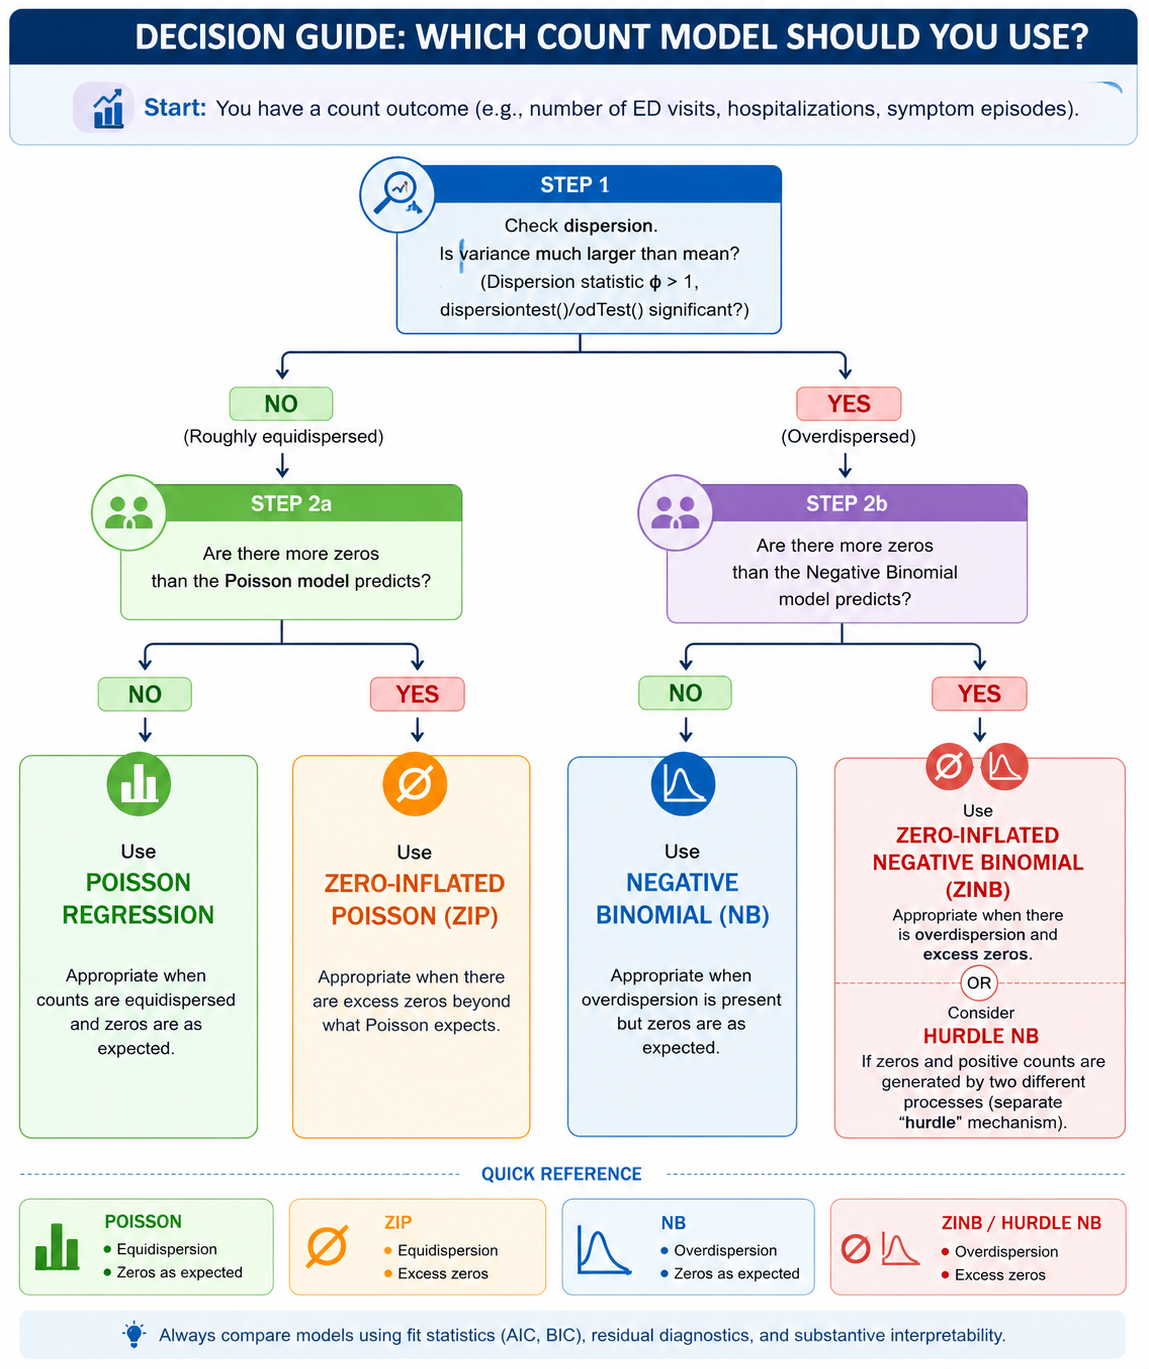
\includegraphics[keepaspectratio]{Section2/Count data analysis/Poisson_pic 1.png}}

\begin{center}\rule{0.5\linewidth}{0.5pt}\end{center}

\section{Summary}\label{summary-8}

Count outcomes in health research (ED visits, hospitalizations, falls,
seizure counts, number of comorbid risk factors) very often violate the
Poisson assumption of equal mean and variance, and frequently show more
zeros than any single, simple distribution predicts. The practical
workflow is:

\begin{enumerate}
\def\labelenumi{\arabic{enumi}.}
\tightlist
\item
  Fit Poisson first; always check the dispersion statistic and compare
  observed vs.~predicted zeros.
\item
  If only overdispersion is present, move to \textbf{Negative Binomial}.
\item
  If only excess zeros are present (counts otherwise well-behaved), move
  to \textbf{Zero-Inflated Poisson}.
\item
  If both problems are present --- the most common situation in practice
  --- move to \textbf{Zero-Inflated Negative Binomial}.
\item
  Use AIC/BIC and the Vuong test to choose between non-nested
  alternatives, and \texttt{odTest()} for the nested Poisson-vs-NB
  comparison; always sanity-check the substantive story (is there really
  a distinct ``not at risk'' subgroup?) rather than choosing a model on
  fit statistics alone.
\item
  Report \textbf{incidence rate ratios (IRRs)} from the count component
  and, for zero-inflated/hurdle models, \textbf{odds ratios} from the
  zero/hurdle component --- these answer two different clinical
  questions (``how many events, given some risk'' vs.~``who is at risk
  at all'') and should be interpreted and reported separately.
\end{enumerate}

\chapter{Survival Analysis}\label{survival-analysis}

\section{Introduction}\label{introduction-8}

Sometime outcome variable may consist of time-to-event consisting of two
components- \textbf{Time and event}. \textbf{Time} means years, months,
weeks or days from the beginning of the follow-up of an individual until
an events occurs. Time can be the age of individual when an event
occurs. It is non negative values. \textbf{Event} means occurrence of
death, disease, incidence, recovery or remission or any experience of
interest that can happen to individual. They are binary. Analytic
alternatives such as \texttt{T-test}, \texttt{ANOVA} ,
\texttt{linear\ models} comparing survival time doesn't incorporate
event component. Logistic regression or other binomial analysis of event
(yes/no) doesn't incorporate time component. In order to incorporate
both component at the same time, there is different analytical approach
which is \textbf{Survival Analysis}. The different examples of survival
analysis problems are:

\begin{itemize}
\item
  Leukemia patients/time in remission (weeks)
\item
  Heart transplants/time until death (months)
\item
  Disease-free cohort/time until heart disease (years)
\end{itemize}

\section{Censoring}\label{censoring}

Censoring occurs when some information about individual survival time is
known, but exact survival time is not known.It can happen: - when study
ended before study participants experienced an event - loss to follow up
- participants withdraw from the study

We should not discard the censored data and if we do, we are ignoring
the partial information available on survival.

\pandocbounded{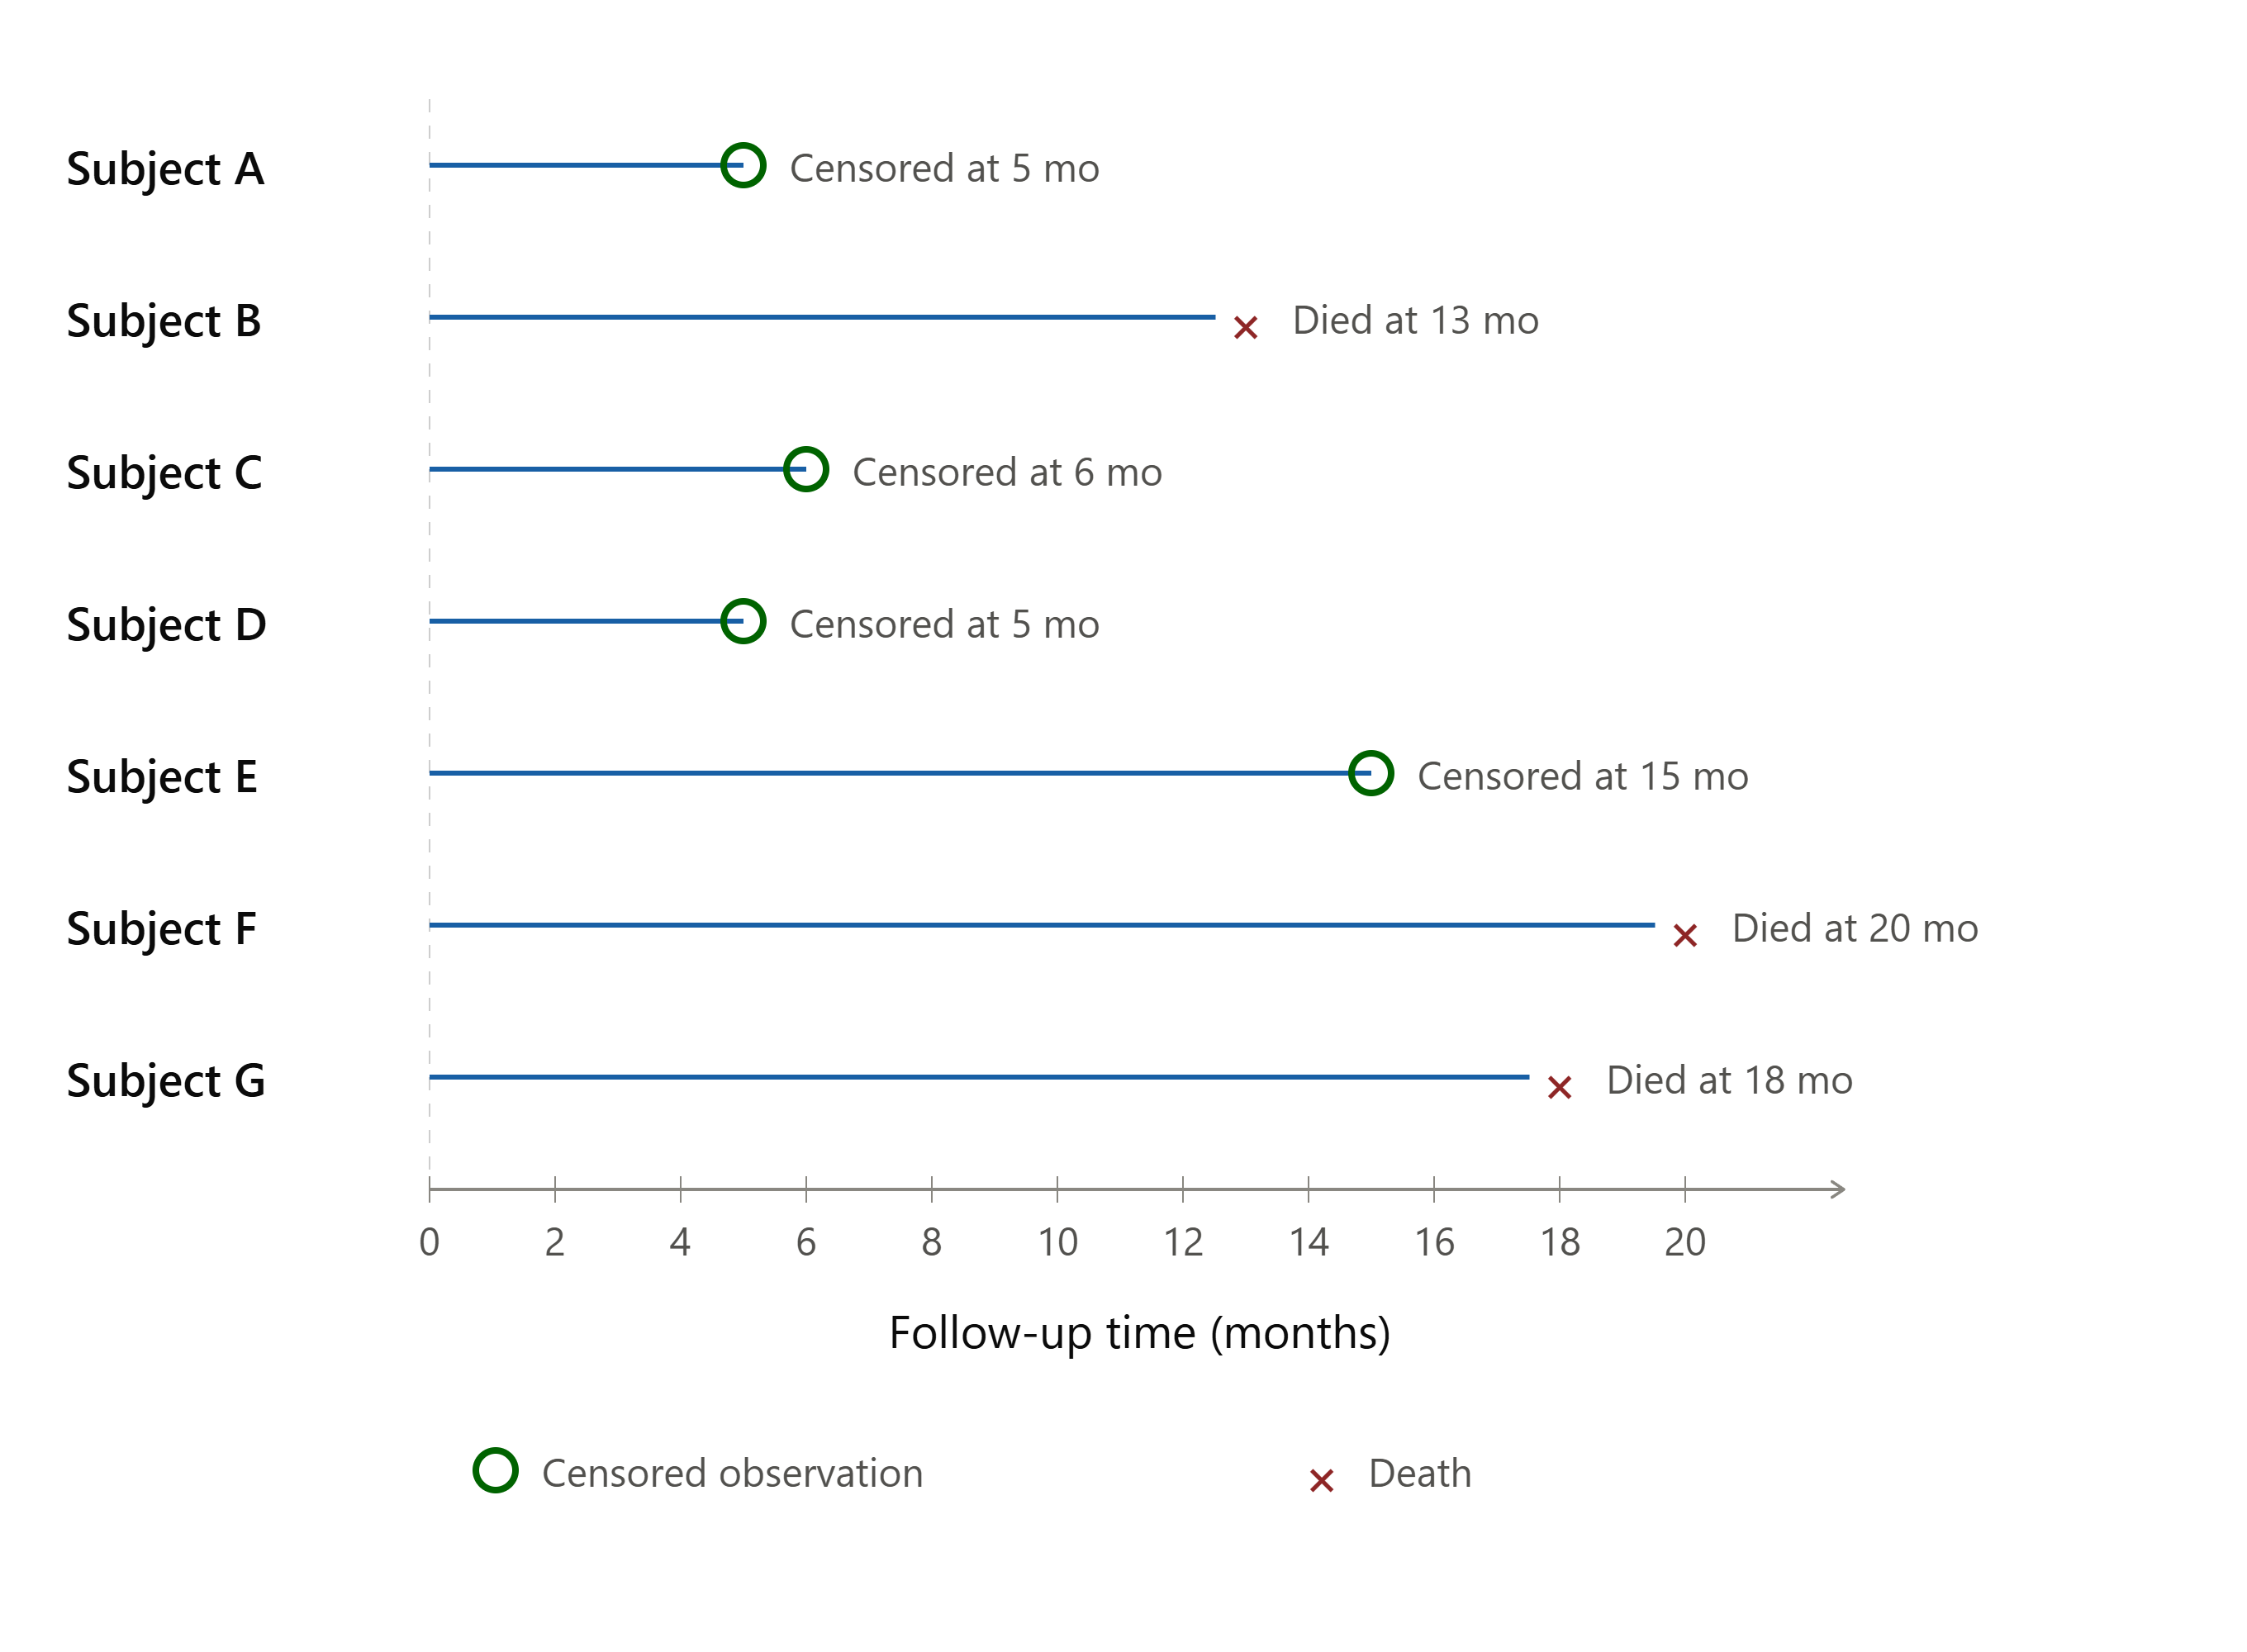
\includegraphics[keepaspectratio]{Section2/Survival analysis/Pictures/survival_pic1.png}}

\subsection{Types}\label{types}

There are three types of censoring

\begin{itemize}
\item
  \textbf{Right Censoring:} It occurs when a true survival time is
  greater than or equal to the observed survival time.
\item
  \textbf{Left Censoring}: It occurs when a true survival time is less
  than or equal to the observed survival time.
\item
  \textbf{Interval censoring}: It occurs when a true survival time lies
  within the know interval but exact time is not known.
\end{itemize}

\subsection{\texorpdfstring{\textbf{Assumptions of
censoring:}}{Assumptions of censoring:}}\label{assumptions-of-censoring}

There are three assumptions of censoring that needed to be considered
during survival data analysis.

\begin{itemize}
\item
  \textbf{Independent censoring:} Within any subgroup of interest, the
  subjects who are censored at time t should be representative of all
  the subjects in that subgroup who remained at risk at time t with
  respect to their survival experience. In other words, censoring is
  independent if it is random within any subgroup of interest.
\item
  \textbf{Random censoring:} Subjects who are censored at time t should
  be representative of all the study subjects who remained at risk at
  time t with respect to their survival experience
\item
  \textbf{Non-informative censoring:} It occurs if the distribution of
  survival times provides no information about the distribution of
  censorship times, and vice versa. Otherwise, the censoring is
  informative. If more than 40\% patients in the treatment arm dropped
  from the study, then censoring is informative about the side effects
  of the treatment.
\end{itemize}

\section{Data structure for survival data
analysis}\label{data-structure-for-survival-data-analysis}

\begin{Shaded}
\begin{Highlighting}[]
\CommentTok{\# install.packages("survival")}
\FunctionTok{library}\NormalTok{(survival)}

\CommentTok{\# cancer data }
\FunctionTok{data}\NormalTok{(}\StringTok{"cancer"}\NormalTok{)}

\FunctionTok{head}\NormalTok{(lung)}
\end{Highlighting}
\end{Shaded}

\begin{verbatim}
#>   inst time status age sex ph.ecog ph.karno pat.karno meal.cal wt.loss
#> 1    3  306      2  74   1       1       90       100     1175      NA
#> 2    3  455      2  68   1       0       90        90     1225      15
#> 3    3 1010      1  56   1       0       90        90       NA      15
#> 4    5  210      2  57   1       1       90        60     1150      11
#> 5    1  883      2  60   1       0      100        90       NA       0
#> 6   12 1022      1  74   1       1       50        80      513       0
\end{verbatim}

\section{Mathematical functions for survival
analysis}\label{mathematical-functions-for-survival-analysis}

There are two mathematical functions for survival analysis:

\begin{itemize}
\item
  Survivorship Function, \texttt{S(t)}
\item
  Hazard Function, \texttt{h(t)}
\end{itemize}

\pandocbounded{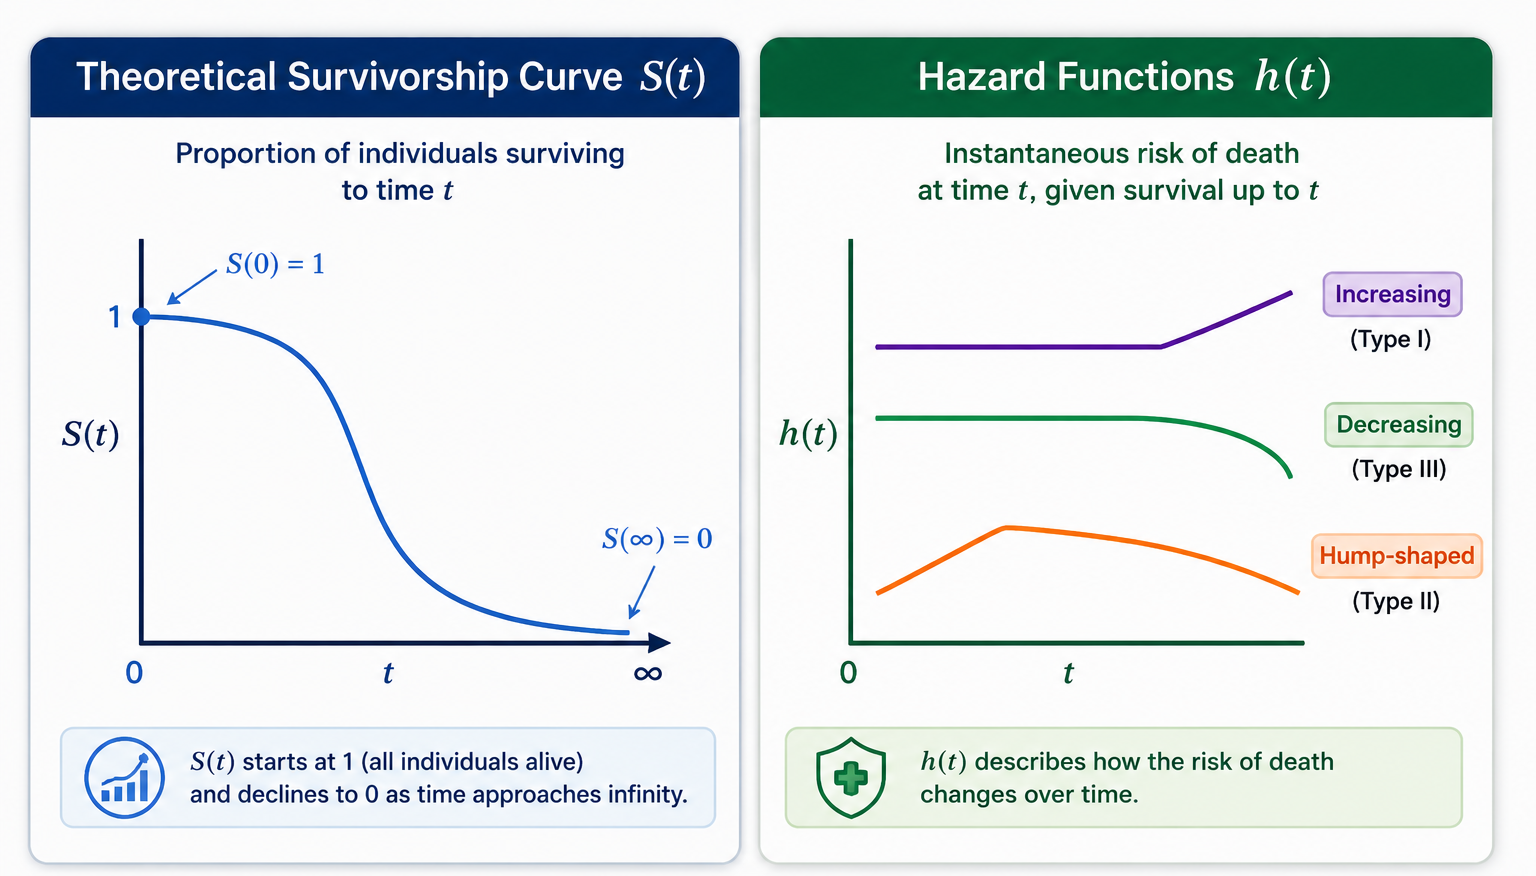
\includegraphics[keepaspectratio]{Section2/Survival analysis/Pictures/survival curve_pic2.png}}

\subsection{\texorpdfstring{\textbf{Survivor
function}}{Survivor function}}\label{survivor-function}

The survivor function \texttt{S(t)} gives the probability that a person
survives longer than some specified time \texttt{t}. That is,
\texttt{S(t)} gives the probability that the random variable \texttt{T}
exceeds the specified time \texttt{t}. The characteristics of survivor
function are:

\begin{itemize}
\item
  non-increasing
\item
  At time \texttt{t\ =\ 0,\ S(t)\ =\ S(0)\ =\ 1}(probability of
  surviving past time 0 is 1)
\item
  At time \texttt{t\ =\ infinity,\ S(t)\ =\ S(infinity)\ =\ 0}
\item
  When using actual data graphs are typically step functions. Because
  the study period is never infinite, it is possible that not everyone
  studied experiences the event. The estimated survivor function may not
  go all the way to zero at the end of the study.
\end{itemize}

\subsection{\texorpdfstring{\textbf{Hazard
function}}{Hazard function}}\label{hazard-function}

Hazard function \texttt{h(t)} measures the instantaneous potential per
unit time for the event to occur, given that the individual has survived
up to time t. While the survivor function focuses on not failing, the
hazard function focuses on failing, that is, on the event occurring. In
some sense, the hazard function can be considered as giving the opposite
side of the information given by the survivor function. Some
characteristics of hazard function are

\begin{itemize}
\item
  It is always non-negative
\item
  It has no upper bound
\item
  Exponential model, Weibull, and log-normal are some mathematical forms
  of hazard functions.
\end{itemize}

\subsection{\texorpdfstring{\textbf{Cummulative hazard},
\texttt{H(t)}:}{Cummulative hazard, H(t):}}\label{cummulative-hazard-ht}

It describes the accumulated risk up to time \texttt{t}.

\[
H(t) = \int_{0}^{t} h(u) d(u)
\]

The expression of survival function in terms of hazard functions:

\[
S(t) =\exp \left [-\int_{0}^{t} h(u) du\right]
\]

The expression of hazard function in terms of survivor function:

\[
h(t) = - \left[ \frac{dS(t) /dt}{S(t)} \right]
\]

\section{Kaplan-Meier Method}\label{kaplan-meier-method}

The survivor function, S(t) gives the probability that an individual
survives longer than a specified time t. In practice, real data are
subject to finite sample size and random variation, so the true survivor
function must be estimated from observed data. One approach is to fit a
parametric model, which imposes a predefined mathematical form on the
data to produce a smooth curve. This offers precision but relies on
strong distributional assumptions that may not hold in real practice. A
non-parametric alternative is the Kaplan-Meier method, which requires
fewer assumptions and allows for a more flexible curve shape. Rather
than forcing the data into a fixed structure, the \textbf{Kaplan-Meier
estimator} let the data ``speak for itself.''

\subsection{The Product-Limit
Estimator}\label{the-product-limit-estimator}

The Kaplan-Meier (KM) estimator is also called the \textbf{product-limit
estimator}, because it is calculated by multiplying together a series of
conditional survival probabilities. Suppose there are \(k\) distinct
observed event times in a sample, ordered as
\(t_{(1)} < t_{(2)} < \dots < t_{(k)}\). At each event time \(t_{(j)}\):

\begin{itemize}
\tightlist
\item
  \(n_j\) = the number of individuals \textbf{at risk} just before
  \(t_{(j)}\) (i.e., still under observation and event-free)
\item
  \(d_j\) = the number of individuals who \textbf{have the event} at
  \(t_{(j)}\)
\end{itemize}

The KM estimator of the survivor function is:

\[
\hat{S}(t) = \prod_{j:\, t_{(j)} \le t} \left(1 - \frac{d_j}{n_j}\right)
\]

In words: the estimated probability of surviving past time \(t\) is the
product, over every event time up to and including \(t\), of the
conditional probability of surviving that event time given survival up
to it. Individuals who are censored are not counted as events, but they
are removed from the risk set at the time they are censored. This is
precisely how the KM method incorporates the partial information
contributed by censored subjects instead of discarding it.

\textbf{Worked example:} Let us consider a small 7-subject data set
which is as below:

\begin{longtable}[]{@{}
  >{\raggedright\arraybackslash}p{(\linewidth - 4\tabcolsep) * \real{0.1389}}
  >{\raggedright\arraybackslash}p{(\linewidth - 4\tabcolsep) * \real{0.0972}}
  >{\raggedright\arraybackslash}p{(\linewidth - 4\tabcolsep) * \real{0.4167}}@{}}
\toprule\noalign{}
\begin{minipage}[b]{\linewidth}\raggedright
Subject
\end{minipage} & \begin{minipage}[b]{\linewidth}\raggedright
Time
\end{minipage} & \begin{minipage}[b]{\linewidth}\raggedright
\textbf{Status}

\textbf{\emph{1: Death/ 0: Censored}}
\end{minipage} \\
\midrule\noalign{}
\endhead
\bottomrule\noalign{}
\endlastfoot
A & 5 & 0 \\
B & 13 & 1 \\
C & 6 & 0 \\
D & 5 & 0 \\
E & 15 & 0 \\
F & 20 & 1 \\
G & 18 & 1 \\
\end{longtable}

\textbf{Step-1:} Order the data by time

\begin{longtable}[]{@{}lll@{}}
\toprule\noalign{}
Subject & Time (in month) & \textbf{Status,} \emph{1: Death/ 0:
Censored} \\
\midrule\noalign{}
\endhead
\bottomrule\noalign{}
\endlastfoot
A & 5 & 0 \\
D & 5 & 0 \\
C & 6 & 0 \\
B & 13 & 1 \\
E & 15 & 0 \\
G & 18 & 1 \\
F & 20 & 1 \\
\end{longtable}

\textbf{Step-2:} Determine the number of subject at risk in the given
time, number of events at that time. Calculate the probability of event
in the risk set by using \(d_j/n_j\) in column 4. There after, calculate
survival probability by substracting the probability of event from 1
like in column 5. At the end, estimate total survival probability by
multiplying survival probabilities from column 5.

\begin{longtable}[]{@{}
  >{\centering\arraybackslash}p{(\linewidth - 10\tabcolsep) * \real{0.1405}}
  >{\centering\arraybackslash}p{(\linewidth - 10\tabcolsep) * \real{0.1322}}
  >{\centering\arraybackslash}p{(\linewidth - 10\tabcolsep) * \real{0.1240}}
  >{\centering\arraybackslash}p{(\linewidth - 10\tabcolsep) * \real{0.0992}}
  >{\centering\arraybackslash}p{(\linewidth - 10\tabcolsep) * \real{0.2727}}
  >{\centering\arraybackslash}p{(\linewidth - 10\tabcolsep) * \real{0.1983}}@{}}
\toprule\noalign{}
\begin{minipage}[b]{\linewidth}\centering
Time \(t_{(j)}\)
\end{minipage} & \begin{minipage}[b]{\linewidth}\centering
At risk \(n_j\)
\end{minipage} & \begin{minipage}[b]{\linewidth}\centering
Events \(d_j\)
\end{minipage} & \begin{minipage}[b]{\linewidth}\centering
\(d_j/n_j\)
\end{minipage} & \begin{minipage}[b]{\linewidth}\centering
survival proportion\(1-d_j/n_j\)
\end{minipage} & \begin{minipage}[b]{\linewidth}\centering
cummulative survival,

\(\hat{S}(t)\)
\end{minipage} \\
\midrule\noalign{}
\endhead
\bottomrule\noalign{}
\endlastfoot
0 & 5 & 0 & 0 & 1.000 & 1.000 \\
13 & 4 & 1 & 0.25 & 0.75 & 0.75 \\
18 & 2 & 1 & 0.50 & 0.50 & 0.375 \\
20 & 1 & 1 & 1 & 0 & 0 \\
\end{longtable}

Censored observations (A and D at month 5, C at 6 months, and E at 15
months) reduce the risk set but do not themselves produce a drop in the
survival curve. The curve only steps down at observed event times.

\begin{Shaded}
\begin{Highlighting}[]
\FunctionTok{library}\NormalTok{(survival)}

\NormalTok{df\_km }\OtherTok{\textless{}{-}} \FunctionTok{data.frame}\NormalTok{(}
  \AttributeTok{subject =} \FunctionTok{c}\NormalTok{(}\StringTok{"A"}\NormalTok{, }\StringTok{"B"}\NormalTok{, }\StringTok{"C"}\NormalTok{, }\StringTok{"D"}\NormalTok{, }\StringTok{"E"}\NormalTok{, }\StringTok{"F"}\NormalTok{, }\StringTok{"G"}\NormalTok{),}
  \AttributeTok{time    =} \FunctionTok{c}\NormalTok{(}\DecValTok{5}\NormalTok{,}\DecValTok{5}\NormalTok{, }\DecValTok{6}\NormalTok{, }\DecValTok{13}\NormalTok{, }\DecValTok{15}\NormalTok{, }\DecValTok{18}\NormalTok{,}\DecValTok{20}\NormalTok{),}
  \AttributeTok{status  =} \FunctionTok{c}\NormalTok{(}\DecValTok{0}\NormalTok{, }\DecValTok{0}\NormalTok{, }\DecValTok{0}\NormalTok{,}\DecValTok{1}\NormalTok{, }\DecValTok{0}\NormalTok{, }\DecValTok{1}\NormalTok{,}\DecValTok{1}\NormalTok{)   }\CommentTok{\# 1 = event (death), 0 = censored}
\NormalTok{)}

\NormalTok{fit\_km }\OtherTok{\textless{}{-}} \FunctionTok{survfit}\NormalTok{(}\FunctionTok{Surv}\NormalTok{(time, status) }\SpecialCharTok{\textasciitilde{}} \DecValTok{1}\NormalTok{, }\AttributeTok{data =}\NormalTok{ df\_km)}
\FunctionTok{summary}\NormalTok{(fit\_km)}
\end{Highlighting}
\end{Shaded}

\begin{verbatim}
#> Call: survfit(formula = Surv(time, status) ~ 1, data = df_km)
#> 
#>  time n.risk n.event survival std.err lower 95% CI upper 95% CI
#>    13      4       1    0.750   0.217       0.4259            1
#>    18      2       1    0.375   0.286       0.0839            1
#>    20      1       1    0.000     NaN           NA           NA
\end{verbatim}

\begin{Shaded}
\begin{Highlighting}[]
\FunctionTok{plot}\NormalTok{(fit\_km, }\AttributeTok{xlab =} \StringTok{"Follow{-}up time (months)"}\NormalTok{, }\AttributeTok{ylab =} \StringTok{"Survival probability"}\NormalTok{,}
     \AttributeTok{main =} \StringTok{"Kaplan{-}Meier Curve"}\NormalTok{, }\AttributeTok{conf.int =} \ConstantTok{FALSE}\NormalTok{, }\AttributeTok{mark.time =} \ConstantTok{TRUE}\NormalTok{)}
\end{Highlighting}
\end{Shaded}

\begin{center}
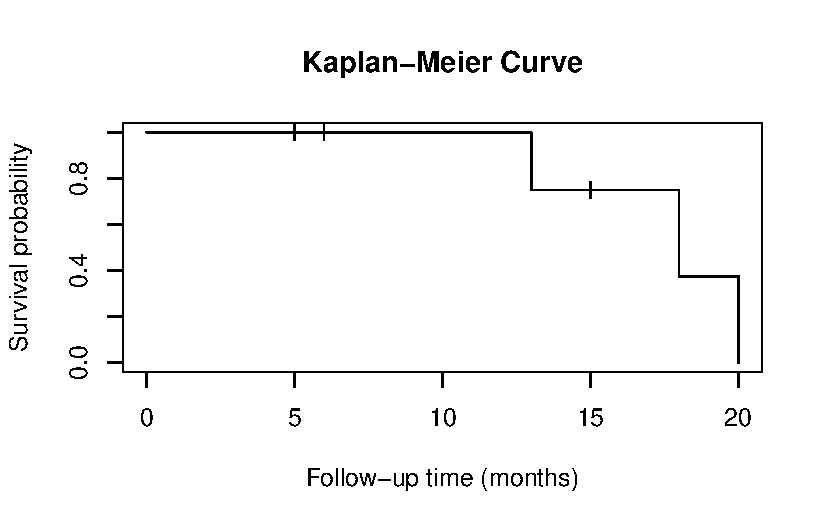
\includegraphics[width=0.85\linewidth,height=\textheight,keepaspectratio]{Section2/Survival analysis/Survival_analysis_files/figure-pdf/unnamed-chunk-2-1.pdf}
\end{center}

\subsection{Standard Error and Confidence Interval for
S(t)}\label{standard-error-and-confidence-interval-for-st}

Because \(\hat{S}(t)\) is estimated from a finite, censored sample, it
has sampling variability that should be reported alongside the point
estimate. The most widely used variance estimator is \textbf{Greenwood's
formula} (Greenwood 1926), derived using a Taylor series (delta method)
approximation:

\[
\widehat{Var}\left[\hat{S}(t)\right] = \left[\hat{S}(t)\right]^2 \sum_{t_{(j)} \le t} \frac{d_j}{n_j(n_j - d_j)}
\]

A large-sample confidence interval for \(S(t)\) follows directly:

\[
\hat{S}(t) \pm z_{1-\alpha/2} \sqrt{\widehat{Var}\left[\hat{S}(t)\right]}
\]

In practice, software typically applies a log or complementary log-log
transformation before constructing the interval and then
back-transforms, which keeps the bounds within \([0,1]\). In R,
\texttt{survfit()} computes Greenwood's standard errors and confidence
limits automatically:

\begin{Shaded}
\begin{Highlighting}[]
\NormalTok{fit\_km\_ci }\OtherTok{\textless{}{-}} \FunctionTok{survfit}\NormalTok{(}\FunctionTok{Surv}\NormalTok{(time, status) }\SpecialCharTok{\textasciitilde{}} \DecValTok{1}\NormalTok{, }\AttributeTok{data =}\NormalTok{ df\_km, }\AttributeTok{conf.type =} \StringTok{"log{-}log"}\NormalTok{)}
\FunctionTok{summary}\NormalTok{(fit\_km\_ci)}
\end{Highlighting}
\end{Shaded}

\begin{verbatim}
#> Call: survfit(formula = Surv(time, status) ~ 1, data = df_km, conf.type = "log-log")
#> 
#>  time n.risk n.event survival std.err lower 95% CI upper 95% CI
#>    13      4       1    0.750   0.217        0.128        0.961
#>    18      2       1    0.375   0.286        0.011        0.808
#>    20      1       1    0.000     NaN           NA           NA
\end{verbatim}

\begin{Shaded}
\begin{Highlighting}[]
\FunctionTok{plot}\NormalTok{(fit\_km\_ci, }\AttributeTok{xlab =} \StringTok{"Follow{-}up time (months)"}\NormalTok{, }\AttributeTok{ylab =} \StringTok{"Survival probability"}\NormalTok{,}
     \AttributeTok{main =} \StringTok{"Kaplan{-}Meier Curve with 95\% CI"}\NormalTok{, }\AttributeTok{conf.int =} \ConstantTok{TRUE}\NormalTok{, }\AttributeTok{mark.time =} \ConstantTok{TRUE}\NormalTok{, }\AttributeTok{col =} \StringTok{"steelblue"}\NormalTok{)}
\end{Highlighting}
\end{Shaded}

\begin{center}
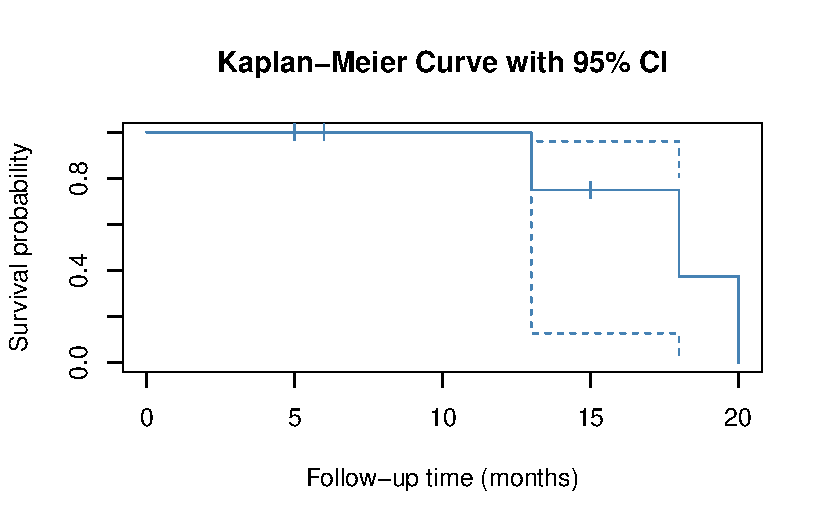
\includegraphics[width=0.85\linewidth,height=\textheight,keepaspectratio]{Section2/Survival analysis/Survival_analysis_files/figure-pdf/unnamed-chunk-3-1.pdf}
\end{center}

\section{Comparing Survival Between Two or More Groups: The Log-Rank
Test}\label{comparing-survival-between-two-or-more-groups-the-log-rank-test}

A common goal in survival analysis is to compare the survival experience
of two or more groups defined by an exposure, treatment, or other
categorical factor. This is done by computing a separate KM curve for
each group and then testing formally whether the underlying survivor
functions differ.

\textbf{Hypotheses:}

\begin{itemize}
\tightlist
\item
  \(H_0\): The survivor functions are identical across groups
\item
  \(H_A\): The survivor functions differ across groups
\end{itemize}

At each distinct event time across the combined data, we can construct a
table of observed events and, under \(H_0\), the number of events
\textbf{expected} in each group (proportional to that group's share of
the risk set at that time). Summing observed minus expected events for a
group across all event times, and appropriately weighting by the
variance, yields the \textbf{log-rank test statistic}:

\[
\chi^2 = \frac{\left(\sum_j (O_{1j} - E_{1j})\right)^2}{\sum_j Var(O_{1j} - E_{1j})} \sim \chi^2_{(g-1)}
\]

where \(g\) is the number of groups being compared. Under \(H_0\), this
statistic follows a chi-square distribution with \(g - 1\) degrees of
freedom (df).

\textbf{Worked example.} In a classical clinical trial, leukemia
patients were randomized to a 6-MP treatment arm versus placebo. In this
study, researcher wanted to answer whether there is difference in
survival between patients with maintenance of chemotherapy versus no
maintenance of chemotherapy. The dataset is as follows:

\begin{Shaded}
\begin{Highlighting}[]
\FunctionTok{data}\NormalTok{(cancer, }\AttributeTok{package =} \StringTok{"survival"}\NormalTok{)}
\FunctionTok{data}\NormalTok{(aml)}
\FunctionTok{head}\NormalTok{(aml)}
\end{Highlighting}
\end{Shaded}

\begin{verbatim}
#>   time status          x
#> 1    9      1 Maintained
#> 2   13      1 Maintained
#> 3   13      0 Maintained
#> 4   18      1 Maintained
#> 5   23      1 Maintained
#> 6   28      0 Maintained
\end{verbatim}

In order to answer the question, we have to perform log rank test. The 5
step hypothesis test is as follows:

\textbf{Step 1: Set up Hypothesis}

\emph{Ho: Two survival functions of chemotherapy Maintained and Not
maintained are identical.}

\emph{Ha: Two survival functions of of Maintained and Not maintained
differ}

\textbf{Step 2: Level of significance}

\[\alpha=0.05\]

\textbf{Step 3: Selection of test statistics}

Since, two survival curve between chemotherapy Maintained and Not
maintained are to be compared, log rank test is the appropriate test to
perform. The formula for log rank test statistics is

\[
\chi^2 = \frac{\left(\sum_j (O_{1j} - E_{1j})\right)^2}{\sum_j Var(O_{1j} - E_{1j})} \sim \chi^2_{(df=1)}
\]

\textbf{Step 4: Calculation of test statistics}

R was used to perform analysis. \texttt{survdiff()} in R performs the
log-rank test directly and reports the chi-square statistic, degrees of
freedom, and p-value. The output of the analysis is as follows:

\begin{Shaded}
\begin{Highlighting}[]
\NormalTok{fit\_aml }\OtherTok{\textless{}{-}} \FunctionTok{survfit}\NormalTok{(}\FunctionTok{Surv}\NormalTok{(time, status) }\SpecialCharTok{\textasciitilde{}}\NormalTok{ x, }\AttributeTok{data =}\NormalTok{ aml)}
\NormalTok{fit\_aml}
\end{Highlighting}
\end{Shaded}

\begin{verbatim}
#> Call: survfit(formula = Surv(time, status) ~ x, data = aml)
#> 
#>                  n events median 0.95LCL 0.95UCL
#> x=Maintained    11      7     31      18      NA
#> x=Nonmaintained 12     11     23       8      NA
\end{verbatim}

\begin{Shaded}
\begin{Highlighting}[]
\FunctionTok{survdiff}\NormalTok{(}\FunctionTok{Surv}\NormalTok{(time, status) }\SpecialCharTok{\textasciitilde{}}\NormalTok{ x, }\AttributeTok{data =}\NormalTok{ aml)}
\end{Highlighting}
\end{Shaded}

\begin{verbatim}
#> Call:
#> survdiff(formula = Surv(time, status) ~ x, data = aml)
#> 
#>                  N Observed Expected (O-E)^2/E (O-E)^2/V
#> x=Maintained    11        7    10.69      1.27       3.4
#> x=Nonmaintained 12       11     7.31      1.86       3.4
#> 
#>  Chisq= 3.4  on 1 degrees of freedom, p= 0.07
\end{verbatim}

\begin{Shaded}
\begin{Highlighting}[]
\FunctionTok{plot}\NormalTok{(fit\_aml, }\AttributeTok{col =} \FunctionTok{c}\NormalTok{(}\StringTok{"blue"}\NormalTok{, }\StringTok{"red"}\NormalTok{), }\AttributeTok{lty =} \DecValTok{1}\SpecialCharTok{:}\DecValTok{2}\NormalTok{,}
     \AttributeTok{xlab =} \StringTok{"Weeks"}\NormalTok{, }\AttributeTok{ylab =} \StringTok{"Survival probability"}\NormalTok{,}
     \AttributeTok{main =} \StringTok{"Kaplan{-}Meier by Maintenance Therapy (aml data)"}\NormalTok{)}
\FunctionTok{legend}\NormalTok{(}\StringTok{"topright"}\NormalTok{, }\AttributeTok{legend =} \FunctionTok{levels}\NormalTok{(aml}\SpecialCharTok{$}\NormalTok{x), }\AttributeTok{col =} \FunctionTok{c}\NormalTok{(}\StringTok{"blue"}\NormalTok{, }\StringTok{"red"}\NormalTok{), }\AttributeTok{lty =} \DecValTok{1}\SpecialCharTok{:}\DecValTok{2}\NormalTok{)}
\end{Highlighting}
\end{Shaded}

\begin{center}
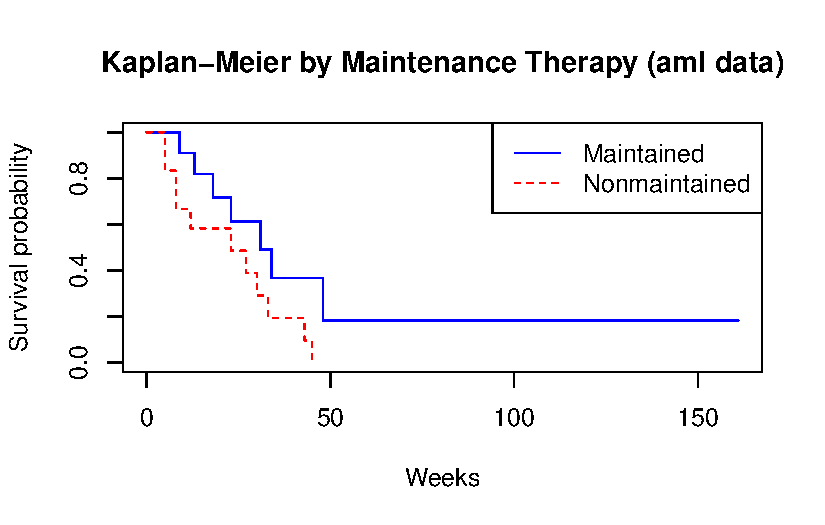
\includegraphics[width=0.85\linewidth,height=\textheight,keepaspectratio]{Section2/Survival analysis/Survival_analysis_files/figure-pdf/unnamed-chunk-5-1.pdf}
\end{center}

\textbf{Manual calculation}

\textbf{Step 1:} Arrange the data in as in the table below. First get
all the time points in assending order. Then, for each time point get
the number of events (m), number of censored observation and number of
subjects at risk (n).

\begin{longtable}[]{@{}
  >{\raggedright\arraybackslash}p{(\linewidth - 12\tabcolsep) * \real{0.1429}}
  >{\raggedright\arraybackslash}p{(\linewidth - 12\tabcolsep) * \real{0.1429}}
  >{\raggedright\arraybackslash}p{(\linewidth - 12\tabcolsep) * \real{0.1429}}
  >{\raggedright\arraybackslash}p{(\linewidth - 12\tabcolsep) * \real{0.1429}}
  >{\raggedright\arraybackslash}p{(\linewidth - 12\tabcolsep) * \real{0.1429}}
  >{\raggedright\arraybackslash}p{(\linewidth - 12\tabcolsep) * \real{0.1429}}
  >{\raggedright\arraybackslash}p{(\linewidth - 12\tabcolsep) * \real{0.1429}}@{}}
\toprule\noalign{}
\begin{minipage}[b]{\linewidth}\raggedright
Time
\end{minipage} & \begin{minipage}[b]{\linewidth}\raggedright
\end{minipage} & \begin{minipage}[b]{\linewidth}\raggedright
\textbf{Maintained}
\end{minipage} & \begin{minipage}[b]{\linewidth}\raggedright
\end{minipage} & \begin{minipage}[b]{\linewidth}\raggedright
\end{minipage} & \begin{minipage}[b]{\linewidth}\raggedright
\textbf{Not maintained}
\end{minipage} & \begin{minipage}[b]{\linewidth}\raggedright
\end{minipage} \\
\midrule\noalign{}
\endhead
\bottomrule\noalign{}
\endlastfoot
& \textbf{Censored (k1)} & \textbf{Events (m1)} & \textbf{At Risk (n1)}
& \textbf{Censored (k2)} & \textbf{Events (m2)} & \textbf{At Risk
(n2)} \\
5 & & & 11 & & 2 & 12 \\
8 & & & 11 & & 2 & 10 \\
9 & & 1 & 11 & & & 8 \\
12 & & & 10 & & 1 & 8 \\
13 & 1 & 1 & 10 & & & 7 \\
16 & & & 8 & 1 & & 7 \\
18 & & 1 & 8 & & & 6 \\
23 & & 1 & 7 & & 1 & 6 \\
27 & & & 6 & & 1 & 5 \\
28 & 1 & & 6 & & & 4 \\
30 & & & 5 & & 1 & 4 \\
31 & & 1 & 5 & & & 3 \\
33 & & & 4 & & 1 & 3 \\
34 & & 1 & 4 & & & 2 \\
43 & & & 3 & & 1 & 2 \\
45 & 1 & & 3 & & 1 & 1 \\
48 & & 1 & 2 & & & 0 \\
161 & 1 & & 1 & & & 0 \\
\end{longtable}

Step-2: Estimate expected number of events for each group using the
formula below\(E_1=\frac{n_1}{(n _1+n_2)}(m_1+m_2)\)

\(E_2=\frac{n_2}{(n_1+n_2)}(m_1+m_2)\) .

\(Variance=\sum Var=\sum\frac{n_1*n_2 (m_1+m_2)(n_1+n_2-m_1-m_2)}{(n_1+n_2)^2 (n_1+n_2-1)}\)

\begin{longtable}[]{@{}
  >{\raggedleft\arraybackslash}p{(\linewidth - 16\tabcolsep) * \real{0.1486}}
  >{\raggedleft\arraybackslash}p{(\linewidth - 16\tabcolsep) * \real{0.0811}}
  >{\raggedleft\arraybackslash}p{(\linewidth - 16\tabcolsep) * \real{0.0811}}
  >{\raggedleft\arraybackslash}p{(\linewidth - 16\tabcolsep) * \real{0.0811}}
  >{\raggedleft\arraybackslash}p{(\linewidth - 16\tabcolsep) * \real{0.0946}}
  >{\raggedleft\arraybackslash}p{(\linewidth - 16\tabcolsep) * \real{0.0946}}
  >{\raggedleft\arraybackslash}p{(\linewidth - 16\tabcolsep) * \real{0.1351}}
  >{\raggedleft\arraybackslash}p{(\linewidth - 16\tabcolsep) * \real{0.1486}}
  >{\raggedleft\arraybackslash}p{(\linewidth - 16\tabcolsep) * \real{0.1351}}@{}}
\toprule\noalign{}
\begin{minipage}[b]{\linewidth}\raggedleft
Time
\end{minipage} & \begin{minipage}[b]{\linewidth}\raggedleft
E₁
\end{minipage} & \begin{minipage}[b]{\linewidth}\raggedleft
E₂
\end{minipage} & \begin{minipage}[b]{\linewidth}\raggedleft
n₁n₂
\end{minipage} & \begin{minipage}[b]{\linewidth}\raggedleft
n1+n2
\end{minipage} & \begin{minipage}[b]{\linewidth}\raggedleft
m1+m2
\end{minipage} & \begin{minipage}[b]{\linewidth}\raggedleft
Var
\end{minipage} & \begin{minipage}[b]{\linewidth}\raggedleft
O₁−E₁
\end{minipage} & \begin{minipage}[b]{\linewidth}\raggedleft
O₂−E₂
\end{minipage} \\
\midrule\noalign{}
\endhead
\bottomrule\noalign{}
\endlastfoot
5 & 0.96 & 1.04 & 132 & 23 & 2 & 0.48 & -0.96 & 0.96 \\
8 & 1.05 & 0.95 & 110 & 21 & 2 & 0.47 & -1.05 & 1.05 \\
9 & 0.58 & 0.42 & 88 & 19 & 1 & 0.24 & 0.42 & -0.42 \\
12 & 0.56 & 0.44 & 80 & 18 & 1 & 0.25 & -0.56 & 0.56 \\
13 & 0.59 & 0.41 & 70 & 17 & 1 & 0.24 & 0.41 & -0.41 \\
16 & 0.00 & 0.00 & 56 & 15 & 0 & 0.00 & 0.00 & 0.00 \\
18 & 0.57 & 0.43 & 48 & 14 & 1 & 0.24 & 0.43 & -0.43 \\
23 & 1.08 & 0.92 & 42 & 13 & 2 & 0.46 & -0.08 & 0.08 \\
27 & 0.55 & 0.45 & 30 & 11 & 1 & 0.25 & -0.55 & 0.55 \\
28 & 0.00 & 0.00 & 24 & 10 & 0 & 0.00 & 0.00 & 0.00 \\
30 & 0.56 & 0.44 & 20 & 9 & 1 & 0.25 & -0.56 & 0.56 \\
31 & 0.63 & 0.38 & 15 & 8 & 1 & 0.23 & 0.38 & -0.38 \\
33 & 0.57 & 0.43 & 12 & 7 & 1 & 0.24 & -0.57 & 0.57 \\
34 & 0.67 & 0.33 & 8 & 6 & 1 & 0.22 & 0.33 & -0.33 \\
43 & 0.60 & 0.40 & 6 & 5 & 1 & 0.24 & -0.60 & 0.60 \\
45 & 0.75 & 0.25 & 3 & 4 & 1 & 0.19 & -0.75 & 0.75 \\
48 & 1.00 & 0.00 & 0 & 2 & 1 & 0.00 & 0.00 & 0.00 \\
161 & 0.00 & 0.00 & 0 & 1 & 0 & & 0.00 & 0.00 \\
\textbf{Total} & & & & & & \textbf{4.01} & \textbf{−3.69} &
\textbf{3.69} \\
\end{longtable}

Log rank test value is calculated using the formula

\[
Log  rank= \frac{(O-E)^2}{Var} = 3.69^2/4.01 =3.4
\]

\textbf{Step 5: Decision and conclusion}

Since p-value is 0.07 which is greater than 0.05 and log rank statistics
is 3.4 which is less than critical value of 3.84, we failed to reject
the null hypothesis. Thus we conclude that there is no significant
difference in two survival curve for chemotherapy Maintained and Not
maintained groups.

\section{Median Survival Time}\label{median-survival-time}

According to National Cancer Institute, \textbf{median survival time} is
the length of time from diagnosis (or start of treatment) at which half
of the patients in a group are still alive({``Definition of Median
Survival - NCI Dictionary of Cancer Terms - NCI''} 2011). It is directly
read from the KM curve as the time at which \(\hat{S}(t) = 0.50\) is
first crossed or first achieved. Because it does not require assuming
the entire tail of the distribution is observed, median survival is
often more useful and more robust to report than mean survival time in
the presence of censoring.

\begin{Shaded}
\begin{Highlighting}[]
\CommentTok{\# Plot}
\FunctionTok{plot}\NormalTok{(fit\_aml,}
     \AttributeTok{col =} \FunctionTok{c}\NormalTok{(}\StringTok{"blue"}\NormalTok{, }\StringTok{"red"}\NormalTok{),}
     \AttributeTok{lty =} \DecValTok{1}\SpecialCharTok{:}\DecValTok{2}\NormalTok{,}
     \AttributeTok{lwd =} \DecValTok{2}\NormalTok{,}
     \AttributeTok{xlab =} \StringTok{"Weeks"}\NormalTok{,}
     \AttributeTok{ylab =} \StringTok{"Survival probability"}\NormalTok{,}
     \AttributeTok{main =} \StringTok{"Kaplan{-}Meier by Maintenance Therapy"}\NormalTok{)}

\FunctionTok{legend}\NormalTok{(}\StringTok{"topright"}\NormalTok{,}
       \AttributeTok{legend =} \FunctionTok{levels}\NormalTok{(aml}\SpecialCharTok{$}\NormalTok{x),}
       \AttributeTok{col =} \FunctionTok{c}\NormalTok{(}\StringTok{"blue"}\NormalTok{, }\StringTok{"red"}\NormalTok{),}
       \AttributeTok{lty =} \DecValTok{1}\SpecialCharTok{:}\DecValTok{2}\NormalTok{,}
       \AttributeTok{lwd =} \DecValTok{2}\NormalTok{,}
       \AttributeTok{bty =} \StringTok{"n"}\NormalTok{)}

\CommentTok{\# Horizontal line at 50\% survival}
\FunctionTok{abline}\NormalTok{(}\AttributeTok{h =} \FloatTok{0.5}\NormalTok{, }\AttributeTok{lty =} \DecValTok{3}\NormalTok{, }\AttributeTok{col =} \StringTok{"darkgray"}\NormalTok{)}

\CommentTok{\# Median survival times}
\NormalTok{med }\OtherTok{\textless{}{-}} \FunctionTok{summary}\NormalTok{(fit\_aml)}\SpecialCharTok{$}\NormalTok{table[, }\StringTok{"median"}\NormalTok{]}

\CommentTok{\# Add vertical lines}
\FunctionTok{abline}\NormalTok{(}\AttributeTok{v =}\NormalTok{ med[}\DecValTok{1}\NormalTok{], }\AttributeTok{col =} \StringTok{"blue"}\NormalTok{, }\AttributeTok{lty =} \DecValTok{3}\NormalTok{)}
\FunctionTok{abline}\NormalTok{(}\AttributeTok{v =}\NormalTok{ med[}\DecValTok{2}\NormalTok{], }\AttributeTok{col =} \StringTok{"red"}\NormalTok{, }\AttributeTok{lty =} \DecValTok{3}\NormalTok{)}

\CommentTok{\# Label median survival times}
\FunctionTok{text}\NormalTok{(med[}\DecValTok{1}\NormalTok{]}\SpecialCharTok{+}\FloatTok{0.5}\NormalTok{, }\FloatTok{0.05}\NormalTok{,}
     \AttributeTok{labels =} \FunctionTok{paste0}\NormalTok{(}\StringTok{"Median = "}\NormalTok{, med[}\DecValTok{1}\NormalTok{]),}
     \AttributeTok{col =} \StringTok{"blue"}\NormalTok{,}
     \AttributeTok{pos =} \DecValTok{4}\NormalTok{,)}

\FunctionTok{text}\NormalTok{(med[}\DecValTok{2}\NormalTok{]}\SpecialCharTok{{-}}\DecValTok{30}\NormalTok{, }\FloatTok{0.05}\NormalTok{,}
     \AttributeTok{labels =} \FunctionTok{paste0}\NormalTok{(}\StringTok{"Median = "}\NormalTok{, med[}\DecValTok{2}\NormalTok{]),}
     \AttributeTok{col =} \StringTok{"red"}\NormalTok{,}
     \AttributeTok{pos =} \DecValTok{4}\NormalTok{)}
\end{Highlighting}
\end{Shaded}

\begin{center}
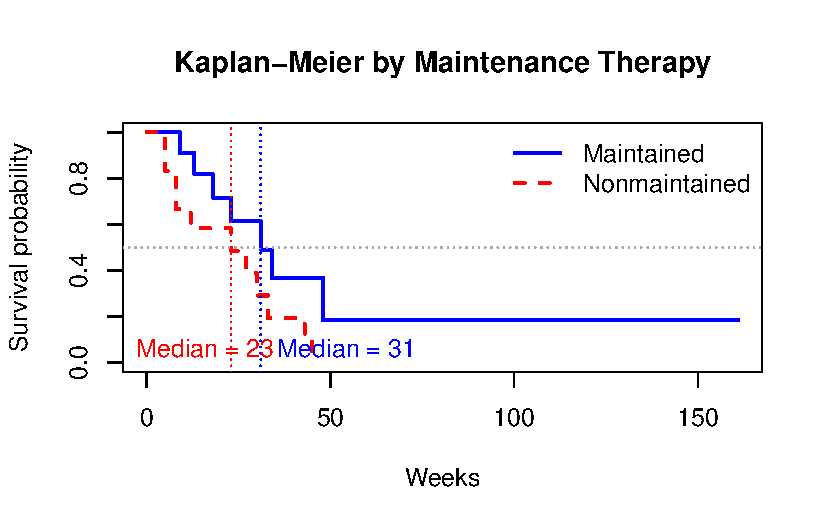
\includegraphics[width=0.85\linewidth,height=\textheight,keepaspectratio]{Section2/Survival analysis/Survival_analysis_files/figure-pdf/unnamed-chunk-6-1.pdf}
\end{center}

If \(\hat{S}(t)\) never falls to 0.50 during the observation period due
to early end of follow up, or treatment is highly effective, median
survival is \textbf{not estimable} and is typically reported as
\textbf{``not reached''}. A 95\% confidence interval for median survival
can also be obtained from the KM curve.

\begin{Shaded}
\begin{Highlighting}[]
\NormalTok{fit\_aml   }\CommentTok{\# printing a survfit object reports median survival and its 95\% CI directly}
\end{Highlighting}
\end{Shaded}

\begin{verbatim}
#> Call: survfit(formula = Surv(time, status) ~ x, data = aml)
#> 
#>                  n events median 0.95LCL 0.95UCL
#> x=Maintained    11      7     31      18      NA
#> x=Nonmaintained 12     11     23       8      NA
\end{verbatim}

The quartiles of survival time divide the estimated survival experience
into four equal parts based on the Kaplan--Meier survival function. They
are defined as the times at which the estimated survival probability
first reaches specific levels.

\begin{itemize}
\item
  \textbf{First quartile (Q1):} The time at which the estimated survival
  probability first falls to \textbf{0.75}. At this point, approximately
  25\% of participants have experienced the event.
\item
  \textbf{Median survival time (Q2):} The time at which the estimated
  survival probability first falls to \textbf{0.50}. By this time,
  approximately 50\% of participants have experienced the event.
\item
  \textbf{Third quartile (Q3):} The time at which the estimated survival
  probability first falls to \textbf{0.25}. By this time, approximately
  75\% of participants have experienced the event.
\end{itemize}

\begin{Shaded}
\begin{Highlighting}[]
\FunctionTok{quantile}\NormalTok{(fit\_aml)}
\end{Highlighting}
\end{Shaded}

\begin{verbatim}
#> $quantile
#>                 25 50 75
#> x=Maintained    18 31 48
#> x=Nonmaintained  8 23 33
#> 
#> $lower
#>                 25 50 75
#> x=Maintained    13 18 34
#> x=Nonmaintained  5  8 27
#> 
#> $upper
#>                 25 50 75
#> x=Maintained    NA NA NA
#> x=Nonmaintained 30 NA NA
\end{verbatim}

\textbf{Interpretation}: The KM estimate indicates that 25\% of patients
experienced the event by 18 weeks(95\%CI: 13, NA) in maintained group,
and by 8 weeks (95\% CI: 5 to 30) in not maintained group. Similarly, it
indicates that 50\% of patients experienced the event by 31
weeks(95\%CI: 18, NA) in maintained group, and by 23 weeks (95\% CI: 8
to NA) in not maintained group. Similarly, it indicates that 75\% of
patients experienced the event by 48 weeks(95\%CI: 34, NA) in maintained
group, and by 33 weeks (95\% CI: 27 to NA) in not maintained group.

\section{The Cox Proportional Hazards
Model}\label{the-cox-proportional-hazards-model}

\subsection{Limitations of the Kaplan-Meier
Approach}\label{limitations-of-the-kaplan-meier-approach}

The KM method and log-rank test are extremely useful, but they have
important limitations:

\begin{itemize}
\tightlist
\item
  They require \textbf{categorical} predictors (grouping variables)
\item
  They do not \textbf{control for covariates} (confounding cannot be
  adjusted for)
\item
  They cannot accommodate \textbf{time-dependent} variables
\end{itemize}

Ordinary linear regression is not a solution either, because it requires
a continuous, uncensored outcome ranging over \((-\infty, \infty)\) ---
not appropriate for time-to-event data with censoring.

\subsection{Sir David Cox and the Proportional Hazards
Model}\label{sir-david-cox-and-the-proportional-hazards-model}

In 1972, the English statistician Sir David Cox introduced the
proportional hazards assumption and, with it, a regression model for
survival data that focuses on the \textbf{hazard function} rather than
on survival time directly (Cox 1972). The Cox model is among the most
heavily cited papers in all of statistics, and the \textbf{Cox
Proportional Hazards (PH) model} remains the most widely used regression
approach for time-to-event data in the health sciences.

The model is built by allowing the hazard for an individual to depend on
a baseline hazard function multiplied by an exponentiated linear
combination of covariates:

\[
h(t, \mathbf{X}) = h_0(t) \exp\left(\beta_1 X_1 + \beta_2 X_2 + \dots + \beta_p X_p\right)
\]

Two features of this formula are essential:

\begin{itemize}
\tightlist
\item
  \(h_0(t)\), the \textbf{baseline hazard function}, depends on \(t\)
  but not on the \(X\)'s. It represents the hazard for an individual
  with all covariates equal to zero, and its functional form is left
  \textbf{completely unspecified}.
\item
  The exponential term \(\exp(\sum \beta_i X_i)\) depends on the \(X\)'s
  but \textbf{not on} \(t\) . These are called time-independent
  covariates, and their effect on the hazard is assumed constant over
  time.
\end{itemize}

Because \(h_0(t)\) is not specified, the Cox model is called
\textbf{semi-parametric}: some structure is assumed for how covariates
act on the hazard, but no particular distributional form is imposed on
survival time itself. This is in contrast to a fully \textbf{parametric}
model, whose functional form is completely specified except for the
values of unknown parameters (discussed later in this chapter). Despite
leaving \(h_0(t)\) unspecified, the Cox model is remarkably robust
regression coefficients, hazard ratios, and adjusted survival curves
obtained from it closely approximate results from the correctly
specified parametric model in a wide range of situations.

\subsection{Assumptions of the Proportional Hazards
Model}\label{assumptions-of-the-proportional-hazards-model}

\begin{enumerate}
\def\labelenumi{\arabic{enumi}.}
\tightlist
\item
  \textbf{Independent observations} across subjects
\item
  \textbf{Independent censoring}
\item
  \textbf{Proportional hazards}: The hazard for one individual is
  proportional to the hazard for any other individual, and this
  proportionality constant does not change over time
\end{enumerate}

\subsection{Fitting the Model: Maximum
Likelihood}\label{fitting-the-model-maximum-likelihood}

The regression coefficients \(\beta_1, \dots, \beta_p\) are estimated
using \textbf{maximum likelihood}, maximizing a \emph{partial}
likelihood function that depends only on the ordering of event times and
the composition of the risk sets, not on the unspecified baseline
hazard. This is analogous to how logistic regression coefficients are
estimated. Because the baseline hazard cancels out of this partial
likelihood, valid inference on the \(\beta\)'s is possible without ever
estimating \(h_0(t)\).

\subsection{The Hazard Ratio}\label{the-hazard-ratio}

Suppose we want to compare the hazard for two individuals (or groups)
with covariate vectors \(\mathbf{X}^*\) and \(\mathbf{X}\). Taking the
ratio of their hazards, the baseline hazard \(h_0(t)\) cancels out
entirely:

\[
\frac{h(t, \mathbf{X}^*)}{h(t, \mathbf{X})} = \frac{h_0(t)\exp(\sum \beta_i X_i^*)}{h_0(t)\exp(\sum \beta_i X_i)} = \exp\left[\sum_i \beta_i (X_i^* - X_i)\right]
\]

This ratio, the \textbf{hazard ratio (HR)}, is the primary measure of
association reported from a Cox model. For a single binary covariate
coded 0/1, comparing \(X_1^*=1\) to \(X_1=0\) gives simply
\(HR = \exp(\beta_1)\). For a continuous covariate,
\(HR = \exp(\beta_1)\) represents the hazard ratio associated with a
\textbf{one-unit increase} in that covariate, holding all other
covariates constant.

\textbf{Interpreting} \(\beta\):

\begin{itemize}
\tightlist
\item
  \(\beta_1\) is the increase in the \emph{log} hazard per one-unit
  increase in \(X_1\)
\item
  \(\exp(\beta_1)\) is the hazard ratio per one-unit increase in \(X_1\)
\item
  \(\beta_1 > 0\) (equivalently \(HR>1\)): increasing \(X_1\) is
  associated with \textbf{increased} hazard (worse survival)
\item
  \(\beta_1 < 0\) (equivalently \(HR<1\)): increasing \(X_1\) is
  associated with \textbf{decreased} hazard (better survival)
\end{itemize}

\textbf{Worked example (single binary predictor).} For lung cancer
data(228 patients), fitting \(h(t)/h_0(t) = \exp(\beta_1 X_1)\) with
\(X_1=1\) for Male produces \(\hat\beta_1 = -0.531\), so
\(\widehat{HR} = \exp(-0.531) = 0.588\) (95\% CI: 0.42, 0.82),
\(\chi^2=10.63\), \(p=0.001\). \textbf{Interpretation:} the hazard of
death for female patients is 41\% lower compared to male patients.

\textbf{Worked example (multiple covariates).} In a lung cancer data,
the hazard of death among female compared to male after adjusting for
age and ph-ecog was determined. , fitting
\(h(t)/h_0(t) = \exp(\beta_1 \text{Sex} + \beta_2 \text{Age}+\beta_3 \text{Ph.ecog})\)
yields \(\widehat{HR}_{sex} = \exp(-0.55) = 0.58\) (95\% CI: 0.41, 0.80)
and \(\widehat{HR}_{age} = \exp(0.011) = 1.01\) (95\% CI: 0.99 to 1.03)
and \(\widehat{HR}_{Ph.ecog} = \exp(0.46) = 1.59\) (95\% CI: 1.27 to
1.99).

\textbf{Interpretation:} After adjustment for age and ECOG performance
status, females had a significantly lower hazard of death than males (HR
= 0.58, 95\% CI: 0.41 to 0.80). Each additional year of age was
associated with an estimated 1\% increase in the hazard of death (HR =
1.01, 95\% CI: 0.99 to 1.03), although this association was not
statistically significant. In contrast, each one-unit increase in ECOG
performance status was associated with a 59\% higher hazard of death (HR
= 1.59, 95\% CI: 1.27 to 1.99), indicating that worse performance status
is an important predictor of mortality after controlling for age and
sex.

\begin{Shaded}
\begin{Highlighting}[]
\FunctionTok{data}\NormalTok{(cancer)}
\FunctionTok{head}\NormalTok{(lung)}
\end{Highlighting}
\end{Shaded}

\begin{verbatim}
#>   inst time status age sex ph.ecog ph.karno pat.karno meal.cal wt.loss
#> 1    3  306      2  74   1       1       90       100     1175      NA
#> 2    3  455      2  68   1       0       90        90     1225      15
#> 3    3 1010      1  56   1       0       90        90       NA      15
#> 4    5  210      2  57   1       1       90        60     1150      11
#> 5    1  883      2  60   1       0      100        90       NA       0
#> 6   12 1022      1  74   1       1       50        80      513       0
\end{verbatim}

\begin{Shaded}
\begin{Highlighting}[]
\CommentTok{\# cleaning}
\NormalTok{lung}\SpecialCharTok{$}\NormalTok{sex }\OtherTok{\textless{}{-}} \FunctionTok{factor}\NormalTok{(lung}\SpecialCharTok{$}\NormalTok{sex, }\AttributeTok{levels =} \FunctionTok{c}\NormalTok{(}\DecValTok{1}\NormalTok{,}\DecValTok{2}\NormalTok{), }\AttributeTok{labels =} \FunctionTok{c}\NormalTok{(}\StringTok{"Male"}\NormalTok{, }\StringTok{"Female"}\NormalTok{))}
\NormalTok{lung}\SpecialCharTok{$}\NormalTok{status }\OtherTok{\textless{}{-}} \FunctionTok{ifelse}\NormalTok{(lung}\SpecialCharTok{$}\NormalTok{status}\SpecialCharTok{==}\DecValTok{1}\NormalTok{, }\DecValTok{0}\NormalTok{, }\DecValTok{1}\NormalTok{)}

\CommentTok{\# Cox model 1}
\NormalTok{cox1 }\OtherTok{\textless{}{-}} \FunctionTok{coxph}\NormalTok{(}\FunctionTok{Surv}\NormalTok{(time, status) }\SpecialCharTok{\textasciitilde{}}\NormalTok{ sex, }\AttributeTok{data =}\NormalTok{ lung)}
\FunctionTok{summary}\NormalTok{(cox1)}
\end{Highlighting}
\end{Shaded}

\begin{verbatim}
#> Call:
#> coxph(formula = Surv(time, status) ~ sex, data = lung)
#> 
#>   n= 228, number of events= 165 
#> 
#>              coef exp(coef) se(coef)      z Pr(>|z|)   
#> sexFemale -0.5310    0.5880   0.1672 -3.176  0.00149 **
#> ---
#> Signif. codes:  0 '***' 0.001 '**' 0.01 '*' 0.05 '.' 0.1 ' ' 1
#> 
#>           exp(coef) exp(-coef) lower .95 upper .95
#> sexFemale     0.588      1.701    0.4237     0.816
#> 
#> Concordance= 0.579  (se = 0.021 )
#> Likelihood ratio test= 10.63  on 1 df,   p=0.001
#> Wald test            = 10.09  on 1 df,   p=0.001
#> Score (logrank) test = 10.33  on 1 df,   p=0.001
\end{verbatim}

\begin{Shaded}
\begin{Highlighting}[]
\CommentTok{\# cox model 2}
\NormalTok{cox2 }\OtherTok{\textless{}{-}} \FunctionTok{coxph}\NormalTok{(}\FunctionTok{Surv}\NormalTok{(time, status) }\SpecialCharTok{\textasciitilde{}}\NormalTok{ age }\SpecialCharTok{+}\NormalTok{ sex }\SpecialCharTok{+}\NormalTok{ ph.ecog, }\AttributeTok{data =}\NormalTok{ lung)}
\FunctionTok{summary}\NormalTok{(cox2)}
\end{Highlighting}
\end{Shaded}

\begin{verbatim}
#> Call:
#> coxph(formula = Surv(time, status) ~ age + sex + ph.ecog, data = lung)
#> 
#>   n= 227, number of events= 164 
#>    (1 observation deleted due to missingness)
#> 
#>                coef exp(coef)  se(coef)      z Pr(>|z|)    
#> age        0.011067  1.011128  0.009267  1.194 0.232416    
#> sexFemale -0.552612  0.575445  0.167739 -3.294 0.000986 ***
#> ph.ecog    0.463728  1.589991  0.113577  4.083 4.45e-05 ***
#> ---
#> Signif. codes:  0 '***' 0.001 '**' 0.01 '*' 0.05 '.' 0.1 ' ' 1
#> 
#>           exp(coef) exp(-coef) lower .95 upper .95
#> age          1.0111     0.9890    0.9929    1.0297
#> sexFemale    0.5754     1.7378    0.4142    0.7994
#> ph.ecog      1.5900     0.6289    1.2727    1.9864
#> 
#> Concordance= 0.637  (se = 0.025 )
#> Likelihood ratio test= 30.5  on 3 df,   p=1e-06
#> Wald test            = 29.93  on 3 df,   p=1e-06
#> Score (logrank) test = 30.5  on 3 df,   p=1e-06
\end{verbatim}

The \texttt{exp(coef)} column in the R output is precisely the estimated
hazard ratio for each covariate, with the associated 95\% confidence
interval given in the \texttt{summary()} output, and the Wald test
p-value indicating whether that covariate is significantly associated
with survival after adjusting for the others in the model.

\section{Assessing the Proportional Hazards
Assumption}\label{assessing-the-proportional-hazards-assumption}

Because the Cox model is \emph{named} after the proportional hazards
assumption, this assumption deserves careful evaluation rather than
being taken for granted. Three general approaches are used to check it.

\subsection{Approach 1: Graphical
Evaluation}\label{approach-1-graphical-evaluation}

\textbf{Log-log survival curves.} A log-log survival curve is obtained
by taking the natural log of the KM survival estimate, twice:
\(-\ln[-\ln \hat{S}(t)]\) (we negate the first log because probabilities
are always \(\le 1\), making \(\ln \hat S(t)\) negative). If the PH
assumption holds for a categorical predictor, the log-log curves for its
categories should be roughly \textbf{parallel} --- non-parallel or
crossing curves suggest a violation.

\begin{Shaded}
\begin{Highlighting}[]
\FunctionTok{plot}\NormalTok{(}\FunctionTok{survfit}\NormalTok{(}\FunctionTok{Surv}\NormalTok{(time, status) }\SpecialCharTok{\textasciitilde{}}\NormalTok{ sex, }\AttributeTok{data =}\NormalTok{ lung), }\AttributeTok{fun =} \StringTok{"cloglog"}\NormalTok{,}
     \AttributeTok{xlab =} \StringTok{"Time in days (log scale)"}\NormalTok{, }\AttributeTok{ylab =} \StringTok{"log({-}log(S(t)))"}\NormalTok{,}
     \AttributeTok{col =} \FunctionTok{c}\NormalTok{(}\StringTok{"blue"}\NormalTok{, }\StringTok{"red"}\NormalTok{), }\AttributeTok{main =} \StringTok{"Log{-}log Survival Curves by Sex (lung data)"}\NormalTok{)}
\FunctionTok{legend}\NormalTok{(}\StringTok{"bottomright"}\NormalTok{, }\AttributeTok{legend =} \FunctionTok{c}\NormalTok{(}\StringTok{"Male"}\NormalTok{, }\StringTok{"Female"}\NormalTok{), }\AttributeTok{col =} \FunctionTok{c}\NormalTok{(}\StringTok{"blue"}\NormalTok{, }\StringTok{"red"}\NormalTok{), }\AttributeTok{lty =} \DecValTok{1}\NormalTok{)}
\end{Highlighting}
\end{Shaded}

\begin{center}
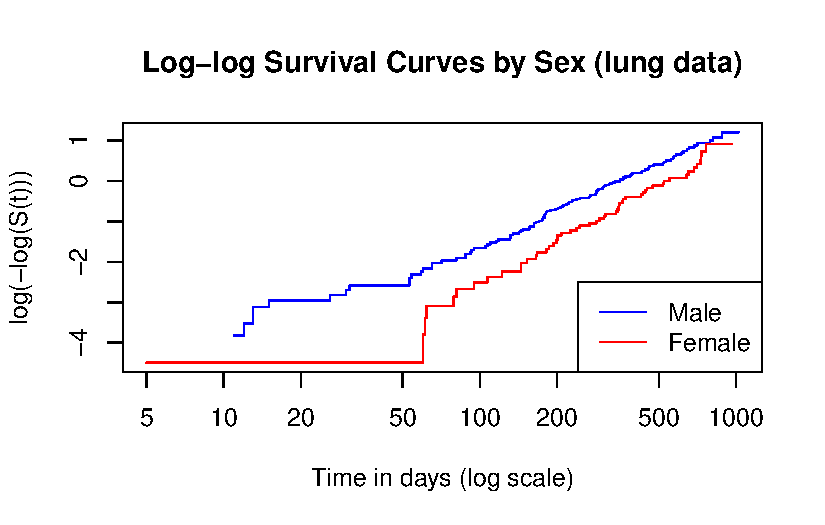
\includegraphics[width=0.85\linewidth,height=\textheight,keepaspectratio]{Section2/Survival analysis/Survival_analysis_files/figure-pdf/unnamed-chunk-10-1.pdf}
\end{center}

\textbf{Observed vs.~expected plots} are a related graphical device: fit
a Cox model containing the predictor of interest, obtain ``expected''
survival curves for each category from the fitted model, and overlay
them on the ``observed'' (KM) curves for the same categories. Close
agreement supports the PH assumption; substantial, systematic divergence
suggests a violation.

Both graphical approaches share a common weakness: judging ``parallel
enough'' or ``close enough'' is inherently subjective. Kleinbaum and
Klein recommend assuming PH is reasonable unless the evidence against it
is fairly convincing.

\subsection{Approach 2: Goodness-of-Fit (Schoenfeld
Residuals)}\label{approach-2-goodness-of-fit-schoenfeld-residuals}

Schoenfeld (1982) proposed a formal hypothesis test based on residuals
which is now called \textbf{Schoenfeld residuals}. It is defined for
each predictor, for each subject who experiences an event. If the PH
assumption holds for a given covariate, its Schoenfeld residuals should
show \textbf{no systematic relationship with time}. The test correlates
the scaled Schoenfeld residuals with (a function of) survival time;
under \(H_0\) (hazards proportional) this correlation is zero.

\begin{itemize}
\tightlist
\item
  \(H_0\): hazards are proportional
\item
  \(H_1\): hazards are not proportional
\item
  Test statistic follows a \(\chi^2\) distribution with 1 df per
  covariate
\end{itemize}

In R, the entire procedure for every covariate in a fitted Cox model
plus a global test is implemented directly by \texttt{cox.zph()}
function.

\begin{Shaded}
\begin{Highlighting}[]
\NormalTok{zph2 }\OtherTok{\textless{}{-}} \FunctionTok{cox.zph}\NormalTok{(cox2)}
\NormalTok{zph2}
\end{Highlighting}
\end{Shaded}

\begin{verbatim}
#>         chisq df    p
#> age     0.188  1 0.66
#> sex     2.305  1 0.13
#> ph.ecog 2.054  1 0.15
#> GLOBAL  4.464  3 0.22
\end{verbatim}

\begin{Shaded}
\begin{Highlighting}[]
\FunctionTok{plot}\NormalTok{(zph2)}
\end{Highlighting}
\end{Shaded}

\begin{center}
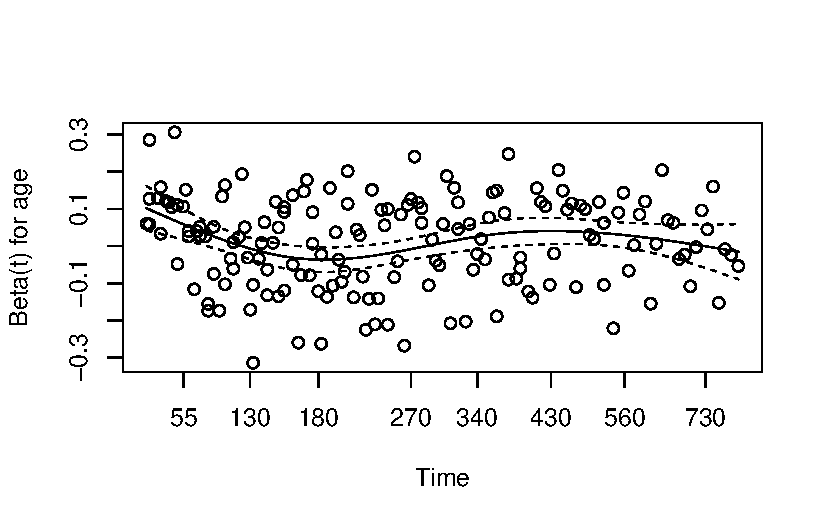
\includegraphics[width=0.85\linewidth,height=\textheight,keepaspectratio]{Section2/Survival analysis/Survival_analysis_files/figure-pdf/unnamed-chunk-11-1.pdf}
\end{center}

\begin{center}
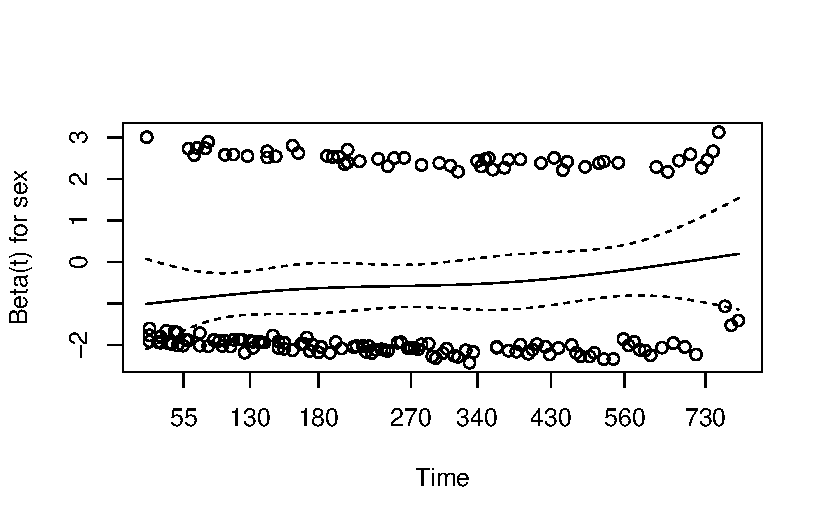
\includegraphics[width=0.85\linewidth,height=\textheight,keepaspectratio]{Section2/Survival analysis/Survival_analysis_files/figure-pdf/unnamed-chunk-11-2.pdf}
\end{center}

\begin{center}
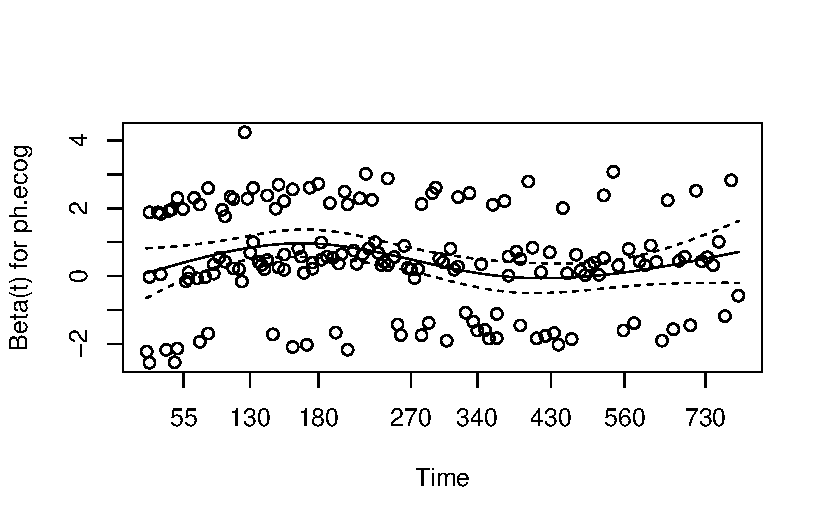
\includegraphics[width=0.85\linewidth,height=\textheight,keepaspectratio]{Section2/Survival analysis/Survival_analysis_files/figure-pdf/unnamed-chunk-11-3.pdf}
\end{center}

A small p-value for any row flags a possible PH violation for that
covariate (or globally). The accompanying plot shows the scaled
Schoenfeld residuals against time with a smoothed trend line. A roughly
flat, horizontal trend supports PH, while a clearly sloped or curved
trend suggests the covariate's effect changes over time.

\subsection{Approach 3: Time-Dependent
Covariates}\label{approach-3-time-dependent-covariates}

A third approach re-fits the Cox model with an added interaction term
between the covariate being assessed and a function of time (e.g.,
\(X \times t\), or a step/``Heaviside'' function of time). If this
interaction term is statistically significant, the PH assumption is
violated for that covariate --- its effect on the hazard changes over
time. This approach doubles as the foundation for the \textbf{extended
Cox model}, discussed later in this chapter.

\section{Model Building: Interaction and
Confounding}\label{model-building-interaction-and-confounding}

\subsection{Assessing Interaction}\label{assessing-interaction}

A statistical \textbf{interaction} (effect modification) is present when
the effect of one exposure on the outcome differs across levels of a
third variable. In the PH model, because we work with hazard ratios (a
multiplicative scale), we are primarily concerned with
\textbf{multiplicative interaction}. No interaction, on this scale,
means:

\[
HR_{11} = HR_{10} \times HR_{01}
\]

That is, the combined effect of two factors acting together equals the
product of their separate effects. This can be tested by adding a
product term to the model:

\[
h(t,\mathbf{X}) = h_0(t)\exp(\beta_1 A + \beta_2 B + \beta_3 A{\times}B), \qquad H_0: \beta_3 = 0
\]

The interaction coefficient can be tested with a Wald test (from the
model output directly) or, preferably, with a \textbf{likelihood ratio
(LR) test} comparing the full (with interaction) and reduced (without
interaction) models:

\[
F_0 = LR_{reduced} - LR_{full} \sim \chi^2_{df}
\]

Statisticians generally consider the LR test to have better statistical
properties than the Wald test for this purpose, though the two usually
agree. When an interaction is statistically significant, hazard ratios
should be reported \emph{separately} for meaningful values or categories
of the effect-modifying variable (or the modifier can be treated as a
stratifying variable, see below), rather than reporting a single
``overall'' hazard ratio that obscures the effect modification.

\subsection{Assessing Confounding}\label{assessing-confounding}

A \textbf{confounder} distorts the observed association between an
exposure and outcome because of its own associations with both. Three
conditions must all hold for a variable to be a confounder: (1) it must
be associated with the outcome, (2) it must be associated with the
exposure, and (3) it must \textbf{not} be an intermediate step on the
causal pathway between exposure and outcome.

From the Cox model, we can compare a \textbf{crude} hazard ratio
(exposure alone) to an \textbf{adjusted} hazard ratio (exposure plus the
potential confounder):

\[
\text{Magnitude of confounding} = \frac{HR_{crude} - HR_{adjusted}}{HR_{adjusted}} \times 100\%
\]

A common rule of thumb (the \textbf{10\% rule}) retains a variable in
the model as a confounder if adjusting for it changes the exposure
hazard ratio by more than 10\%. When several potential confounders are
being screened, they are typically evaluated one at a time against the
fully adjusted model.

It is worth distinguishing the two phenomena clearly:
\textbf{confounding} is a distortion of the true association caused by
an imbalance in another risk factor --- the stratum-specific estimates
will be similar to each other but different from the crude estimate.
\textbf{Effect modification}, by contrast, is a real biological/clinical
phenomenon in which the stratum-specific estimates genuinely differ from
one another; it should be described and reported, not ``adjusted away.''

\subsection{Model-Building Strategy (E-V-W
Framework)}\label{model-building-strategy-e-v-w-framework}

When the primary study goal is a valid \textbf{exposure--disease (E-D)}
association (as opposed to pure outcome prediction), Kleinbaum and Klein
recommend a structured strategy rather than automated stepwise
procedures:

\begin{enumerate}
\def\labelenumi{\arabic{enumi}.}
\tightlist
\item
  \textbf{Variable specification} --- designate one exposure of interest
  (\(E\)), and classify remaining covariates as potential confounders
  (\(V_1,\dots,V_p\)) and/or potential effect modifiers
  (\(W_1,\dots,W_p\)), based on subject-matter knowledge, prior
  literature, and (optionally) causal diagrams
\item
  \textbf{Check the PH assumption} for each variable
\item
  \textbf{Assess interaction} (\(E \times W\) terms), retaining
  significant ones
\item
  \textbf{Assess confounding} among the \(V\)'s using the 10\% rule, in
  a \textbf{hierarchically well-formulated (HWF)} framework --- i.e., if
  a higher-order term (like \(E{\times}V_1{\times}V_2\)) is retained,
  all its lower-order components (\(E\), \(V_1\), \(V_2\),
  \(E{\times}V_1\), \(E{\times}V_2\), \(V_1{\times}V_2\)) must also
  remain in the model, so that hypothesis tests do not depend
  arbitrarily on how variables happen to be coded
\end{enumerate}

When the goal is instead a good \textbf{prediction} model rather than a
specific E-D estimate, standard iterative procedures (forward selection,
backward elimination, stepwise regression) are more appropriate.

\subsection{Evaluating Predictive Accuracy: The
C-Statistic}\label{evaluating-predictive-accuracy-the-c-statistic}

The \textbf{concordance index (C-statistic)}, also known as Harrell's C,
measures how well a fitted survival model discriminates between subjects
who fail sooner versus later, based on their predicted risk scores
\(\hat\eta_i = \sum \hat\beta_k X_{ik}\). For every comparable pair of
subjects, the pair is \textbf{concordant} if the subject with the higher
risk score has the shorter observed survival time. The C-statistic is
the proportion of concordant pairs among all pairs that can be
evaluated:

\begin{itemize}
\tightlist
\item
  \(C = 0.5\): no better than chance
\item
  \(C = 1.0\): perfect discrimination
\end{itemize}

\begin{Shaded}
\begin{Highlighting}[]
\CommentTok{\# Harrels\textquotesingle{} C index}
\FunctionTok{concordance}\NormalTok{(cox2)}
\end{Highlighting}
\end{Shaded}

\begin{verbatim}
#> Call:
#> concordance.coxph(object = cox2)
#> 
#> n= 227 
#> Concordance= 0.6371 se= 0.02507
#> concordant discordant     tied.x     tied.y    tied.xy 
#>      12544       7117        126         28          0
\end{verbatim}

Because heavy censoring can bias the ordinary C-statistic, \textbf{Uno's
C-statistic} uses inverse probability of censoring weighting (IPCW) and
is generally preferred when censoring exceeds roughly 30\%. The R-code
to calculate Uno's C-statistic is as follows:

\begin{Shaded}
\begin{Highlighting}[]
\CommentTok{\#install.packages("survAUC")}

\FunctionTok{library}\NormalTok{(survAUC)}

\CommentTok{\# Cox model}
\NormalTok{cox1 }\OtherTok{\textless{}{-}} \FunctionTok{coxph}\NormalTok{(}\FunctionTok{Surv}\NormalTok{(time, status) }\SpecialCharTok{\textasciitilde{}}\NormalTok{ age }\SpecialCharTok{+}\NormalTok{ sex,}
              \AttributeTok{data =}\NormalTok{ lung)}

\FunctionTok{UnoC}\NormalTok{(}
  \FunctionTok{Surv}\NormalTok{(lung}\SpecialCharTok{$}\NormalTok{time, lung}\SpecialCharTok{$}\NormalTok{status),}
  \FunctionTok{Surv}\NormalTok{(lung}\SpecialCharTok{$}\NormalTok{time, lung}\SpecialCharTok{$}\NormalTok{status),}
  \FunctionTok{predict}\NormalTok{(cox1, }\AttributeTok{type =} \StringTok{"lp"}\NormalTok{) }\CommentTok{\# linear predictor}
\NormalTok{)}
\end{Highlighting}
\end{Shaded}

\begin{verbatim}
#> [1] 0.5848518
\end{verbatim}

\section{The Stratified Cox Model}\label{the-stratified-cox-model}

When one or more categorical covariates clearly violate the PH
assumption, but we still want to control for them, the
\textbf{stratified Cox (SC) model} offers a solution. Suppose
\(X_1,\dots,X_p\) satisfy the PH assumption and \(Z_1,\dots,Z_k\) do
not. We form a single stratification variable \(Z^*\) from combinations
of categories of the \(Z\)'s, and fit:

\[
h_g(t,\mathbf{X}) = h_{0g}(t)\exp\left(\sum_i \beta_i X_i\right), \qquad g = 1,\dots,\text{(number of strata)}
\]

Each stratum \(g\) is allowed its \textbf{own, unspecified baseline
hazard function} \(h_{0g}(t)\), but the regression coefficients for
\(X_1,\dots,X_p\) are assumed to be the \textbf{same across strata} ---
this is the ``no-interaction'' assumption underlying the SC model. Its
major advantage is that it lets us \textbf{control for} a variable that
violates PH; its major limitation is that we can \textbf{no longer
estimate a hazard ratio for the stratification variable itself}.

The no-interaction assumption can (and should) be checked with a
likelihood ratio test comparing a model that allows separate
coefficients per stratum against the common-coefficient stratified
model. If interaction is present, it is generally better to fit separate
models within each stratum than to force a single stratified Cox model.

\begin{Shaded}
\begin{Highlighting}[]
\FunctionTok{data}\NormalTok{(veteran)}
\FunctionTok{head}\NormalTok{(veteran)}
\end{Highlighting}
\end{Shaded}

\begin{verbatim}
#>   trt celltype time status karno diagtime age prior
#> 1   1 squamous   72      1    60        7  69     0
#> 2   1 squamous  411      1    70        5  64    10
#> 3   1 squamous  228      1    60        3  38     0
#> 4   1 squamous  126      1    60        9  63    10
#> 5   1 squamous  118      1    70       11  65    10
#> 6   1 squamous   10      1    20        5  49     0
\end{verbatim}

\begin{Shaded}
\begin{Highlighting}[]
\CommentTok{\# check PH assumption first}
\NormalTok{cox\_v }\OtherTok{\textless{}{-}} \FunctionTok{coxph}\NormalTok{(}\FunctionTok{Surv}\NormalTok{(time, status) }\SpecialCharTok{\textasciitilde{}}\NormalTok{ trt }\SpecialCharTok{+}\NormalTok{ age }\SpecialCharTok{+} \FunctionTok{factor}\NormalTok{(celltype), }\AttributeTok{data =}\NormalTok{ veteran)}
\FunctionTok{cox.zph}\NormalTok{(cox\_v)}
\end{Highlighting}
\end{Shaded}

\begin{verbatim}
#>                   chisq df     p
#> trt               0.892  1 0.345
#> age               1.231  1 0.267
#> factor(celltype)  9.213  3 0.027
#> GLOBAL           12.598  5 0.027
\end{verbatim}

\begin{Shaded}
\begin{Highlighting}[]
\CommentTok{\# stratify on the variable(s) that violate PH (here, illustratively, celltype)}
\NormalTok{cox\_strat }\OtherTok{\textless{}{-}} \FunctionTok{coxph}\NormalTok{(}\FunctionTok{Surv}\NormalTok{(time, status) }\SpecialCharTok{\textasciitilde{}}\NormalTok{ trt }\SpecialCharTok{+}\NormalTok{ age }\SpecialCharTok{+} \FunctionTok{strata}\NormalTok{(celltype), }\AttributeTok{data =}\NormalTok{ veteran)}
\FunctionTok{summary}\NormalTok{(cox\_strat)}
\end{Highlighting}
\end{Shaded}

\begin{verbatim}
#> Call:
#> coxph(formula = Surv(time, status) ~ trt + age + strata(celltype), 
#>     data = veteran)
#> 
#>   n= 137, number of events= 128 
#> 
#>         coef exp(coef) se(coef)     z Pr(>|z|)
#> trt 0.159202  1.172575 0.203399 0.783    0.434
#> age 0.002104  1.002106 0.009820 0.214    0.830
#> 
#>     exp(coef) exp(-coef) lower .95 upper .95
#> trt     1.173     0.8528    0.7871     1.747
#> age     1.002     0.9979    0.9830     1.022
#> 
#> Concordance= 0.522  (se = 0.032 )
#> Likelihood ratio test= 0.77  on 2 df,   p=0.7
#> Wald test            = 0.77  on 2 df,   p=0.7
#> Score (logrank) test = 0.77  on 2 df,   p=0.7
\end{verbatim}

In this formulation, \texttt{celltype} no longer produces its own hazard
ratio --- it defines four separate baseline hazards, one per cell type
--- while \texttt{trt} and \texttt{age} retain interpretable,
celltype-adjusted hazard ratios.

\section{The Extended Cox Model for Time-Dependent
Covariates}\label{the-extended-cox-model-for-time-dependent-covariates}

\subsection{Time-Dependent Variables}\label{time-dependent-variables}

A \textbf{time-dependent} variable is one whose value for a given
subject can change over the course of follow-up, in contrast to a
time-independent variable, which is fixed at baseline. Time-dependent
variables arise in two ways:

\begin{enumerate}
\def\labelenumi{\arabic{enumi}.}
\tightlist
\item
  \textbf{Inherently time-dependent} variables change by nature ---
  smoking status, employment status, air pollution exposure, or (the
  classic example) heart-transplant status for a patient awaiting a
  transplant. A patient's transplant indicator is 0 until the day of
  transplant and 1 thereafter, for the remainder of follow-up.
\item
  \textbf{Defined} time-dependent variables are constructed specifically
  to test or relax the PH assumption for a time-independent predictor
  whose \emph{effect}, not its value, appears to change over time.
\end{enumerate}

Time can enter the extended Cox model in three ways: (1) directly, as
\(X \times t\); (2) as a general function \(X \times g(t)\) (e.g.,
\(g(t)=\log t\)); or (3) as a \textbf{Heaviside function} --- a step
function that lets a covariate's effect take one value before a
pre-specified time \(t_0\) and a different value after it:

\[
h(t,\mathbf{X}) = h_0(t)\exp\left(\beta_1 X + \delta \, X\, g(t)\right), \qquad g(t) = \begin{cases} 0 & t < t_0 \\ 1 & t \ge t_0 \end{cases}
\]

Before \(t_0\) the effect of \(X\) is \(\beta_1\); at or after \(t_0\)
it becomes \(\beta_1 + \delta\). Heaviside functions are attractive
because they are simple to interpret and model an abrupt,
known-timepoint change in effect (e.g., after a protocol amendment); a
general (continuous) function of time is more appropriate when the
change in effect is gradual.

Because the general hazard-ratio formula now involves the difference in
time-dependent covariate values \emph{at time} \(t\), \textbf{the hazard
ratio itself becomes a function of time} --- this is precisely why a
model with time-dependent covariates no longer satisfies (and doesn't
need to satisfy) the ordinary PH assumption. Estimation still proceeds
by maximum (partial) likelihood, and Wald/LR tests and confidence
intervals are constructed the same way as for the standard Cox model,
though the risk sets used to build the partial likelihood are more
complex.

\subsection{A Worked Example in R: The Stanford Heart Transplant
Data}\label{a-worked-example-in-r-the-stanford-heart-transplant-data}

The \texttt{heart} data set built into the \textbf{survival} package is
the classic time-dependent covariate example --- patients awaiting a
heart transplant, where \texttt{transplant} status changes value partway
through a patient's follow-up time. The data are already arranged in
\emph{counting-process} \texttt{(start,\ stop,\ event)} format, which is
the standard way R represents time-dependent covariates:

\begin{Shaded}
\begin{Highlighting}[]
\FunctionTok{data}\NormalTok{(heart)}
\FunctionTok{head}\NormalTok{(heart)}
\end{Highlighting}
\end{Shaded}

\begin{verbatim}
#>   start stop event        age      year surgery transplant id
#> 1     0   50     1 -17.155373 0.1232033       0          0  1
#> 2     0    6     1   3.835729 0.2546201       0          0  2
#> 3     0    1     0   6.297057 0.2655715       0          0  3
#> 4     1   16     1   6.297057 0.2655715       0          1  3
#> 5     0   36     0  -7.737166 0.4900753       0          0  4
#> 6    36   39     1  -7.737166 0.4900753       0          1  4
\end{verbatim}

\begin{Shaded}
\begin{Highlighting}[]
\NormalTok{cox\_td }\OtherTok{\textless{}{-}} \FunctionTok{coxph}\NormalTok{(}\FunctionTok{Surv}\NormalTok{(start, stop, event) }\SpecialCharTok{\textasciitilde{}}\NormalTok{ age }\SpecialCharTok{+}\NormalTok{ surgery }\SpecialCharTok{+}\NormalTok{ transplant, }\AttributeTok{data =}\NormalTok{ heart)}
\FunctionTok{summary}\NormalTok{(cox\_td)}
\end{Highlighting}
\end{Shaded}

\begin{verbatim}
#> Call:
#> coxph(formula = Surv(start, stop, event) ~ age + surgery + transplant, 
#>     data = heart)
#> 
#>   n= 172, number of events= 75 
#> 
#>                 coef exp(coef) se(coef)      z Pr(>|z|)  
#> age          0.03054   1.03101  0.01389  2.198   0.0279 *
#> surgery     -0.77333   0.46147  0.35967 -2.150   0.0315 *
#> transplant1  0.01610   1.01623  0.30859  0.052   0.9584  
#> ---
#> Signif. codes:  0 '***' 0.001 '**' 0.01 '*' 0.05 '.' 0.1 ' ' 1
#> 
#>             exp(coef) exp(-coef) lower .95 upper .95
#> age            1.0310     0.9699     1.003    1.0595
#> surgery        0.4615     2.1670     0.228    0.9339
#> transplant1    1.0162     0.9840     0.555    1.8606
#> 
#> Concordance= 0.6  (se = 0.036 )
#> Likelihood ratio test= 10.72  on 3 df,   p=0.01
#> Wald test            = 9.68  on 3 df,   p=0.02
#> Score (logrank) test = 10  on 3 df,   p=0.02
\end{verbatim}

Each subject contributes one row per time interval during which their
covariate values are constant; a subject who receives a transplant
partway through follow-up contributes (at least) two rows --- one with
\texttt{transplant\ =\ 0} up to the transplant date, and one with
\texttt{transplant\ =\ 1} from the transplant date onward. This
\texttt{(start,\ stop)} counting-process layout is the general mechanism
R uses to fit both the extended Cox model and the Heaviside-function
formulation described above (a Heaviside term is simply an additional
column, computed as the covariate multiplied by an indicator for
\texttt{stop\ \textgreater{}=\ t0}, included alongside the
time-independent version of the same covariate).

\section{Parametric Survival Models}\label{parametric-survival-models}

\subsection{Motivation}\label{motivation}

The Cox model is semi-parametric --- it leaves the baseline hazard
\(h_0(t)\) completely unspecified. A \textbf{parametric survival model},
by contrast, assumes survival time follows a specific probability
distribution (exponential, Weibull, log-logistic, log-normal, or
generalized gamma, among others), fully specified except for a small
number of unknown parameters. Once a probability density function
\(f(t)\) is specified, the corresponding survival function
\(S(t) = \int_t^\infty f(u)\,du\) and hazard function
\(h(t) = f(t)/S(t)\) follow directly --- specifying any one of the three
(\(f\), \(S\), or \(h\)) determines the other two.

Parametric models produce smooth theoretical survival curves (rather
than the step functions typical of KM and Cox-adjusted estimates), and,
if the distributional assumption is reasonable, they yield more precise
and more easily summarized estimates (e.g., closed-form expressions for
median survival). The trade-off is the added distributional assumption
itself, which should be checked.

\subsection{The Exponential Model}\label{the-exponential-model}

The simplest parametric survival model assumes a \textbf{constant
hazard} over time, \(h(t) = \lambda\), which implies
\(S(t) = \exp(-\lambda t)\). Re-parameterizing
\(\lambda = \exp(\beta_0 + \beta_1 X_1 + \dots)\) allows covariates to
be incorporated. Note that assuming a constant hazard is a \emph{much
stronger} assumption than proportional hazards --- if the hazards
themselves are constant, their ratio is automatically constant, but a
constant ratio does not require either hazard individually to be
constant.

\subsection{The Weibull Model}\label{the-weibull-model}

The \textbf{Weibull distribution} is the most widely used parametric
survival model. It generalizes the exponential by adding a shape
parameter \(p\) that governs whether the hazard increases, decreases, or
stays constant over time (the exponential is the special case \(p=1\)).
A convenient property of the Weibull model is that \textbf{if the AFT
assumption holds, the PH assumption also holds} for a
Weibull-distributed outcome --- making it something of a bridge between
the two frameworks. Another useful property: \(\log[-\log S(t)]\) is
linear in \(\log(t)\) under a Weibull model, which provides a simple
graphical check --- plotting the log-log KM curves against \(\log(t)\)
for each group should produce roughly straight, parallel lines if the
Weibull (and PH) assumptions are reasonable.

\subsection{Accelerated Failure Time (AFT)
Models}\label{accelerated-failure-time-aft-models}

Many parametric survival models --- including the exponential, Weibull,
and log-logistic --- can be formulated as \textbf{accelerated failure
time (AFT)} models, an alternative to the proportional-hazards
framework. Where the PH model assumes covariates act multiplicatively on
the \textbf{hazard}, the AFT model assumes covariates act
multiplicatively on \textbf{survival time} itself:

\[
\log T = \alpha_0 + \alpha_1 X_1 + \alpha_2 X_2 + \dots + \alpha_p X_p + \sigma\varepsilon
\]

where \(\sigma\) is a scale parameter and \(\varepsilon\) is a random
error term whose assumed distribution determines the AFT model family
(e.g., a standard extreme-value distribution for \(\varepsilon\) gives
the Weibull/exponential AFT model).

A helpful intuition: it is often said dogs age about seven times faster
than humans, so that a dog surviving to age 10 is, in some sense,
``equivalent'' to a human surviving to age 70. Formally,
\(S_{dog}(t) = S_{human}(7t)\) --- dogs are accelerated through life by
a factor of 7 relative to humans. The AFT model quantifies exactly this
kind of ``stretching'' or ``contraction'' of the survival time scale as
a function of covariates. The key measure of association is the
\textbf{acceleration factor}, \(\gamma = \exp(\alpha_1)\): it is the
ratio of times at which two groups reach the \emph{same} survival
probability. An acceleration factor greater than 1 for an exposure means
that exposure is \textbf{beneficial} (survival time is stretched out)
--- note this is the opposite direction from a hazard ratio, where
\(HR>1\) indicates \textbf{harm}.

\textbf{Interpreting AFT coefficients:} increasing \(X_1\) by one unit,
holding other covariates fixed, changes the expected log survival time
by \(\alpha_1\), i.e., it multiplies expected survival time by
\(\exp(\alpha_1)\). If \(\alpha_1 > 0\) survival time increases (better
survival); if \(\alpha_1 < 0\) survival time decreases (worse survival)
--- again the reverse sign convention from the Cox hazard ratio.

\textbf{Worked example.} In the leukemia remission-time trial, fitting
an exponential AFT model with treatment as the sole predictor gives an
acceleration factor of \(\gamma = \exp(1.5266) = 4.60\) --- treatment
stretches expected remission time by a factor of 4.6 relative to
placebo. Fitting the richer Weibull AFT model to the same data gives a
similar acceleration factor (3.55, 95\% CI 1.93--6.53) with a slightly
better model fit, since the Weibull relaxes the strong constant-hazard
assumption of the exponential model.

\begin{Shaded}
\begin{Highlighting}[]
\NormalTok{aft\_exp  }\OtherTok{\textless{}{-}} \FunctionTok{survreg}\NormalTok{(}\FunctionTok{Surv}\NormalTok{(time, status) }\SpecialCharTok{\textasciitilde{}}\NormalTok{ age }\SpecialCharTok{+}\NormalTok{ sex, }\AttributeTok{data =}\NormalTok{ lung, }\AttributeTok{dist =} \StringTok{"exponential"}\NormalTok{)}
\FunctionTok{summary}\NormalTok{(aft\_exp)}
\end{Highlighting}
\end{Shaded}

\begin{verbatim}
#> 
#> Call:
#> survreg(formula = Surv(time, status) ~ age + sex, data = lung, 
#>     dist = "exponential")
#>                Value Std. Error     z      p
#> (Intercept)  6.84061    0.58748 11.64 <2e-16
#> age         -0.01562    0.00911 -1.72  0.086
#> sexFemale    0.48093    0.16709  2.88  0.004
#> 
#> Scale fixed at 1 
#> 
#> Exponential distribution
#> Loglik(model)= -1156.1   Loglik(intercept only)= -1162.3
#>  Chisq= 12.48 on 2 degrees of freedom, p= 0.002 
#> Number of Newton-Raphson Iterations: 4 
#> n= 228
\end{verbatim}

\begin{Shaded}
\begin{Highlighting}[]
\NormalTok{aft\_weib }\OtherTok{\textless{}{-}} \FunctionTok{survreg}\NormalTok{(}\FunctionTok{Surv}\NormalTok{(time, status) }\SpecialCharTok{\textasciitilde{}}\NormalTok{ age }\SpecialCharTok{+}\NormalTok{ sex, }\AttributeTok{data =}\NormalTok{ lung, }\AttributeTok{dist =} \StringTok{"weibull"}\NormalTok{)}
\FunctionTok{summary}\NormalTok{(aft\_weib)}
\end{Highlighting}
\end{Shaded}

\begin{verbatim}
#> 
#> Call:
#> survreg(formula = Surv(time, status) ~ age + sex, data = lung, 
#>     dist = "weibull")
#>                Value Std. Error     z       p
#> (Intercept)  6.65694    0.44752 14.88 < 2e-16
#> age         -0.01226    0.00696 -1.76  0.0781
#> sexFemale    0.38209    0.12748  3.00  0.0027
#> Log(scale)  -0.28230    0.06188 -4.56 5.1e-06
#> 
#> Scale= 0.754 
#> 
#> Weibull distribution
#> Loglik(model)= -1147.1   Loglik(intercept only)= -1153.9
#>  Chisq= 13.59 on 2 degrees of freedom, p= 0.0011 
#> Number of Newton-Raphson Iterations: 5 
#> n= 228
\end{verbatim}

Note that \texttt{survreg()} reports coefficients on the \(\log T\)
scale directly (the AFT parameterization), which is the \emph{opposite}
sign convention from \texttt{coxph()}'s hazard-ratio scale --- a
positive \texttt{survreg} coefficient means \textbf{longer} survival,
while a positive \texttt{coxph} coefficient means \textbf{higher hazard}
(shorter survival). Model fit for a parametric model can be checked
graphically using \textbf{Cox-Snell residuals}: if the model is
correctly specified, the Cox-Snell residuals should themselves behave
like a censored sample from a unit-exponential distribution, i.e., a
plot of the cumulative hazard of the residuals against the residuals
should fall approximately on a straight line through the origin with
slope 1.

\subsection{Comparing AFT and Cox
Regression}\label{comparing-aft-and-cox-regression}

\begin{longtable}[]{@{}
  >{\raggedright\arraybackslash}p{(\linewidth - 4\tabcolsep) * \real{0.3333}}
  >{\raggedright\arraybackslash}p{(\linewidth - 4\tabcolsep) * \real{0.3333}}
  >{\raggedright\arraybackslash}p{(\linewidth - 4\tabcolsep) * \real{0.3333}}@{}}
\toprule\noalign{}
\begin{minipage}[b]{\linewidth}\raggedright
\end{minipage} & \begin{minipage}[b]{\linewidth}\raggedright
AFT Model
\end{minipage} & \begin{minipage}[b]{\linewidth}\raggedright
Cox PH Model
\end{minipage} \\
\midrule\noalign{}
\endhead
\bottomrule\noalign{}
\endlastfoot
Assumption & Specific error distribution (exponential, Weibull, etc.) &
Proportional hazards \\
Coefficient interpretation & Change in (log) survival time & Change in
log hazard (hazard ratio) \\
Baseline hazard & Fully specified & Left unspecified \\
Typical use & Comparing survival times directly; some high-dimensional /
variable-selection settings & The default choice in most biomedical
survival studies \\
\end{longtable}

\section{Design and Sample Size Considerations for Survival
Studies}\label{design-and-sample-size-considerations-for-survival-studies}

Designing a study with a time-to-event outcome requires answering
several linked questions: how many subjects are needed, how long should
the accrual (recruitment) period be, how long should follow-up continue
after accrual ends, and how should the analysis handle subjects who
switch treatment groups partway through?

\subsection{Basic Statistical
Principles}\label{basic-statistical-principles}

As with any hypothesis test, four quantities are linked in sample-size
planning for survival studies:

\begin{itemize}
\tightlist
\item
  \(\alpha\) (Type I error) --- the probability of rejecting \(H_0\)
  when it is actually true; conventionally set to 0.05
\item
  \textbf{Power (}\(1-\beta\)) --- the probability of correctly
  rejecting \(H_0\) when a true difference exists; power increases with
  sample size
\item
  \textbf{Effect size (}\(\Delta\)) --- the magnitude of the true
  difference between groups, expressed as a hazard ratio, a ratio of
  survival probabilities, or a ratio of median survival times; larger
  effect sizes require fewer subjects to detect
\item
  \textbf{Sample size / number of events} --- the quantity we are
  usually solving for
\end{itemize}

A key distinction in survival study design is between the \textbf{study
size} (\(N\), total number of participants enrolled) and the
\textbf{number of events} (\(NEV\), the number of participants who
actually experience the outcome during the study). Because the
statistical power of a survival analysis is driven primarily by the
number of \emph{events} observed --- not simply the number of subjects
enrolled --- sample size calculations typically proceed in two stages:
first determine the required number of events, then back-calculate the
total study size needed to observe that many events given the assumed
event rate, accrual period, and follow-up duration.

\subsection{Freedman's Formula for the Number of
Events}\label{freedmans-formula-for-the-number-of-events}

Assuming proportional hazards, a widely used formula (Freedman, 1982)
for the number of events required to detect a hazard ratio (or
equivalently a ratio of median survival times) \(\Delta\) with two-sided
significance level \(\alpha\) and power \(1-\beta\) is:

\[
NEV = \frac{\left(z_{1-\alpha/2} + z_{1-\beta}\right)^2 (\Delta+1)^2}{(\Delta - 1)^2}
\]

\begin{Shaded}
\begin{Highlighting}[]
\NormalTok{alpha }\OtherTok{\textless{}{-}} \FloatTok{0.05}
\NormalTok{power }\OtherTok{\textless{}{-}} \FloatTok{0.80}
\NormalTok{delta }\OtherTok{\textless{}{-}} \DecValTok{2}          \CommentTok{\# e.g., a 2{-}fold increase in median survival time (14 vs 7 months)}

\NormalTok{z\_alpha }\OtherTok{\textless{}{-}} \FunctionTok{qnorm}\NormalTok{(}\DecValTok{1} \SpecialCharTok{{-}}\NormalTok{ alpha }\SpecialCharTok{/} \DecValTok{2}\NormalTok{)}
\NormalTok{z\_beta  }\OtherTok{\textless{}{-}} \FunctionTok{qnorm}\NormalTok{(power)}

\NormalTok{NEV }\OtherTok{\textless{}{-}}\NormalTok{ ((z\_alpha }\SpecialCharTok{+}\NormalTok{ z\_beta)}\SpecialCharTok{\^{}}\DecValTok{2} \SpecialCharTok{*}\NormalTok{ (delta }\SpecialCharTok{+} \DecValTok{1}\NormalTok{)}\SpecialCharTok{\^{}}\DecValTok{2}\NormalTok{) }\SpecialCharTok{/}\NormalTok{ (delta }\SpecialCharTok{{-}} \DecValTok{1}\NormalTok{)}\SpecialCharTok{\^{}}\DecValTok{2}
\NormalTok{NEV}
\end{Highlighting}
\end{Shaded}

\begin{verbatim}
#> [1] 70.63992
\end{verbatim}

For example, detecting a doubling of median survival time (7 vs.~14
months) with 80\% power at \(\alpha=0.05\) requires roughly 71 events
(per the formula above); accruing events faster than anticipated
increases the realized power for a fixed effect size.

Converting the required number of events into a required study size
additionally requires the length of the accrual period, the length of
additional follow-up after accrual closes, and an assumed event-time
distribution (exponential is common, since it yields simple closed-form
results and is usually adequate for planning purposes even if it will
not be assumed for the final analysis). In practice, these calculations
are performed by software. Dedicated tools such as
\texttt{powerSurvEpi::ssizeCT.default()}, \texttt{Hmisc::cpower()}, or
the \texttt{gsDesign} package implement these formulas (including
accrual/follow-up adjustments) directly; SAS's \texttt{PROC\ POWER} with
\texttt{twosamplesurvival} performs the equivalent calculation.

\subsection{Additional Design
Considerations}\label{additional-design-considerations}

\begin{itemize}
\tightlist
\item
  \textbf{Unequal allocation.} Sample size formulas can be adapted for
  allocation ratios other than 1:1 (e.g., 2:1 randomization).
\item
  \textbf{Loss to follow-up.} If a known or anticipated proportion of
  subjects will be lost before experiencing the event, the required
  study size (with full follow-up) must be inflated accordingly.
\item
  \textbf{Treatment cross-over.} Under the intention-to-treat (ITT)
  principle, subjects are analyzed according to their original
  randomized assignment regardless of whether they later switch
  treatments --- this preserves the benefits of randomization. However,
  cross-over dilutes the observed effect size, so the study size must be
  inflated by a \textbf{cross-over adjustment / sample size inflation
  factor} to maintain the originally planned power.
\end{itemize}

\subsection{Multiple Comparisons}\label{multiple-comparisons}

Whenever a study involves several hypothesis tests on the same data set
(pairwise group comparisons, multiple outcomes, subgroup analyses), the
probability of at least one \textbf{false positive} across the whole
family of tests --- the \textbf{familywise (experimentwise) error rate}
--- climbs well above the nominal per-test \(\alpha\). For example, with
10 independent tests each conducted at \(\alpha=0.05\), the probability
of at least one Type I error is \(1-(1-0.05)^{10} \approx 0.40\).

Common corrections for the familywise error rate include:

\begin{itemize}
\tightlist
\item
  \textbf{Bonferroni}: use \(\alpha/m\) for \(m\) comparisons (simple
  but conservative)
\item
  \textbf{Šidák}: \(\alpha_{SID} = 1-(1-\alpha)^{1/m}\) (slightly less
  conservative than Bonferroni)
\item
  \textbf{Benjamini-Hochberg (FDR)}: controls the \emph{expected
  proportion} of false discoveries rather than the probability of any
  false discovery, and is less conservative when many tests are
  performed
\end{itemize}

\begin{Shaded}
\begin{Highlighting}[]
\NormalTok{raw\_p }\OtherTok{\textless{}{-}} \FunctionTok{c}\NormalTok{(}\FloatTok{0.01}\NormalTok{, }\FloatTok{0.02}\NormalTok{, }\FloatTok{0.04}\NormalTok{, }\FloatTok{0.20}\NormalTok{, }\FloatTok{0.03}\NormalTok{)}
\FunctionTok{p.adjust}\NormalTok{(raw\_p, }\AttributeTok{method =} \StringTok{"bonferroni"}\NormalTok{)}
\end{Highlighting}
\end{Shaded}

\begin{verbatim}
#> [1] 0.05 0.10 0.20 1.00 0.15
\end{verbatim}

\begin{Shaded}
\begin{Highlighting}[]
\FunctionTok{p.adjust}\NormalTok{(raw\_p, }\AttributeTok{method =} \StringTok{"BH"}\NormalTok{)}
\end{Highlighting}
\end{Shaded}

\begin{verbatim}
#> [1] 0.05 0.05 0.05 0.20 0.05
\end{verbatim}

Not all statisticians agree that adjustment is always appropriate ---
Rothman (1990) famously argued that routine multiplicity adjustment
sacrifices power (inflating Type II error) in exchange for protecting
the null hypothesis, which may not always be the right trade-off.
Whether (and how) to adjust should be guided by the study's goals, its
exploratory vs.~confirmatory nature, and the relative costs of false
positive versus false negative conclusions.

\section{Competing Risks}\label{competing-risks}

\subsection{The Problem}\label{the-problem}

\textbf{Competing risks} arise when each subject can experience only one
of several distinct types of event, and the occurrence of one type
precludes (or ``competes with'') observing the others. Classic examples
include a patient who can die of cancer \emph{or} of cardiovascular
disease (but not both), or a soldier who can die in combat \emph{or} in
a traffic accident. When competing risks are present, the standard
KM/Cox toolbox needs modification, because:

\begin{itemize}
\tightlist
\item
  Treating competing events simply as ``censored'' observations in a
  cause-specific analysis requires assuming the competing risks are
  \textbf{independent} of the event of interest
\item
  The KM curve for a specific cause, computed this way, can have a
  questionable interpretation --- in an extreme example, if an entire
  cohort dies simultaneously in an unrelated accident, the KM
  ``survival'' curve for, say, cancer death remains at 1 (implying no
  one ever dies of cancer), which is clearly misleading
\end{itemize}

\subsection{Cause-Specific Hazards (Method
1)}\label{cause-specific-hazards-method-1}

The most common approach fits a \textbf{separate Cox model for each
event type}, treating all \emph{other} event types (in addition to
ordinary loss-to-follow-up and study-end censoring) as censored
observations. This gives a cause-specific hazard ratio for each event
type, e.g., \(h_{ca}(t,\mathbf{X}) = h_{0,ca}(t)\exp(\sum \beta_i X_i)\)
for cancer death specifically. This approach is intuitive and easy to
implement but still assumes the competing risks are independent, and the
resulting ``1 minus cause-specific KM'' curve overestimates the true
cumulative probability of that specific event.

\subsection{Cumulative Incidence Functions (Fine \&
Gray)}\label{cumulative-incidence-functions-fine-gray}

The \textbf{cumulative incidence function (CIF)} is a more appropriate
summary curve in the presence of competing risks. It starts at 0 (rather
than 1) and increases as events of the specific type of interest occur,
appropriately accounting for the fact that subjects who experience a
competing event are no longer at risk for the event of interest. Unlike
the naive ``1 − KM'' curve, the CIF does not require assuming the
competing risks are independent. \textbf{Gray's test} (1988) is a
log-rank-like test for comparing CIFs between groups (again without the
independence assumption, though it does not adjust for covariates), and
the \textbf{Fine-Gray model} (1999) extends the proportional-hazards
framework to model the CIF (technically, the ``subdistribution hazard'')
directly as a function of covariates.

R's \texttt{survival} package supports multi-state \texttt{Surv()}
objects that directly produce cumulative incidence estimates via
\texttt{survfit()}. Using the built-in \texttt{mgus2} data set
(monoclonal gammopathy patients who may progress to a plasma cell
malignancy or die of another cause before progressing --- two competing
risks):

\begin{Shaded}
\begin{Highlighting}[]
\FunctionTok{data}\NormalTok{(mgus2)}
\FunctionTok{str}\NormalTok{(mgus2)}
\end{Highlighting}
\end{Shaded}

\begin{verbatim}
#> 'data.frame':    1384 obs. of  11 variables:
#>  $ id    : num  1 2 3 4 5 6 7 8 9 10 ...
#>  $ age   : num  88 78 94 68 90 90 89 87 86 79 ...
#>   ..- attr(*, "label")= chr "AGE AT mgus_sp"
#>  $ sex   : Factor w/ 2 levels "F","M": 1 1 2 2 1 2 1 1 1 1 ...
#>   ..- attr(*, "label")= chr "Sex"
#>   ..- attr(*, "format")= chr "$desex"
#>  $ dxyr  : num  1981 1968 1980 1977 1973 ...
#>  $ hgb   : num  13.1 11.5 10.5 15.2 10.7 12.9 10.5 12.3 14.5 9.4 ...
#>  $ creat : num  1.3 1.2 1.5 1.2 0.8 1 0.9 1.2 0.9 1.1 ...
#>  $ mspike: num  0.5 2 2.6 1.2 1 0.5 1.3 1.6 2.4 2.3 ...
#>   ..- attr(*, "label")= chr "SEP SPIKE AT mgus_sp"
#>  $ ptime : num  30 25 46 92 8 4 151 2 57 136 ...
#>  $ pstat : num  0 0 0 0 0 0 0 0 0 0 ...
#>  $ futime: num  30 25 46 92 8 4 151 2 57 136 ...
#>  $ death : num  1 1 1 1 1 1 1 1 0 1 ...
\end{verbatim}

\begin{Shaded}
\begin{Highlighting}[]
\NormalTok{mgus2}\SpecialCharTok{$}\NormalTok{etime }\OtherTok{\textless{}{-}} \FunctionTok{with}\NormalTok{(mgus2, }\FunctionTok{ifelse}\NormalTok{(pstat }\SpecialCharTok{==} \DecValTok{0}\NormalTok{, futime, ptime))}
\NormalTok{mgus2}\SpecialCharTok{$}\NormalTok{event }\OtherTok{\textless{}{-}} \FunctionTok{with}\NormalTok{(mgus2, }\FunctionTok{ifelse}\NormalTok{(pstat }\SpecialCharTok{==} \DecValTok{0}\NormalTok{, }\DecValTok{2} \SpecialCharTok{*}\NormalTok{ death, }\DecValTok{1}\NormalTok{))}
\NormalTok{mgus2}\SpecialCharTok{$}\NormalTok{event }\OtherTok{\textless{}{-}} \FunctionTok{factor}\NormalTok{(mgus2}\SpecialCharTok{$}\NormalTok{event, }\DecValTok{0}\SpecialCharTok{:}\DecValTok{2}\NormalTok{, }\AttributeTok{labels =} \FunctionTok{c}\NormalTok{(}\StringTok{"censor"}\NormalTok{, }\StringTok{"pcm"}\NormalTok{, }\StringTok{"death"}\NormalTok{))}

\NormalTok{fit\_cif }\OtherTok{\textless{}{-}} \FunctionTok{survfit}\NormalTok{(}\FunctionTok{Surv}\NormalTok{(etime, event) }\SpecialCharTok{\textasciitilde{}}\NormalTok{ sex, }\AttributeTok{data =}\NormalTok{ mgus2)}
\NormalTok{fit\_cif}
\end{Highlighting}
\end{Shaded}

\begin{verbatim}
#> Call: survfit(formula = Surv(etime, event) ~ sex, data = mgus2)
#> 
#>                n nevent     rmean se(rmean)*
#> sex=F, (s0)  631      0 139.01247   5.682211
#> sex=M, (s0)  753      0 122.97693   5.742051
#> sex=F, pcm   631     59  42.77078   4.495519
#> sex=M, pcm   753     56  31.82962   4.185262
#> sex=F, death 631    370 242.21675   6.745244
#> sex=M, death 753    490 269.19344   6.630760
#>    *restricted mean time in state (max time = 424 )
\end{verbatim}

\begin{Shaded}
\begin{Highlighting}[]
\FunctionTok{plot}\NormalTok{(fit\_cif, }\AttributeTok{col =} \FunctionTok{c}\NormalTok{(}\DecValTok{1}\NormalTok{, }\DecValTok{1}\NormalTok{, }\DecValTok{2}\NormalTok{, }\DecValTok{2}\NormalTok{), }\AttributeTok{lty =} \FunctionTok{c}\NormalTok{(}\DecValTok{1}\NormalTok{, }\DecValTok{2}\NormalTok{, }\DecValTok{1}\NormalTok{, }\DecValTok{2}\NormalTok{),}
     \AttributeTok{xlab =} \StringTok{"Years from diagnosis"}\NormalTok{, }\AttributeTok{ylab =} \StringTok{"Cumulative incidence"}\NormalTok{,}
     \AttributeTok{main =} \StringTok{"Cumulative Incidence of PCM and Death, by Sex"}\NormalTok{)}
\FunctionTok{legend}\NormalTok{(}\StringTok{"topleft"}\NormalTok{, }\AttributeTok{legend =} \FunctionTok{c}\NormalTok{(}\StringTok{"F: PCM"}\NormalTok{, }\StringTok{"F: Death"}\NormalTok{, }\StringTok{"M: PCM"}\NormalTok{, }\StringTok{"M: Death"}\NormalTok{),}
       \AttributeTok{col =} \FunctionTok{c}\NormalTok{(}\DecValTok{1}\NormalTok{, }\DecValTok{2}\NormalTok{, }\DecValTok{1}\NormalTok{, }\DecValTok{2}\NormalTok{), }\AttributeTok{lty =} \FunctionTok{c}\NormalTok{(}\DecValTok{1}\NormalTok{, }\DecValTok{1}\NormalTok{, }\DecValTok{2}\NormalTok{, }\DecValTok{2}\NormalTok{), }\AttributeTok{cex =} \FloatTok{0.8}\NormalTok{)}
\end{Highlighting}
\end{Shaded}

\begin{center}
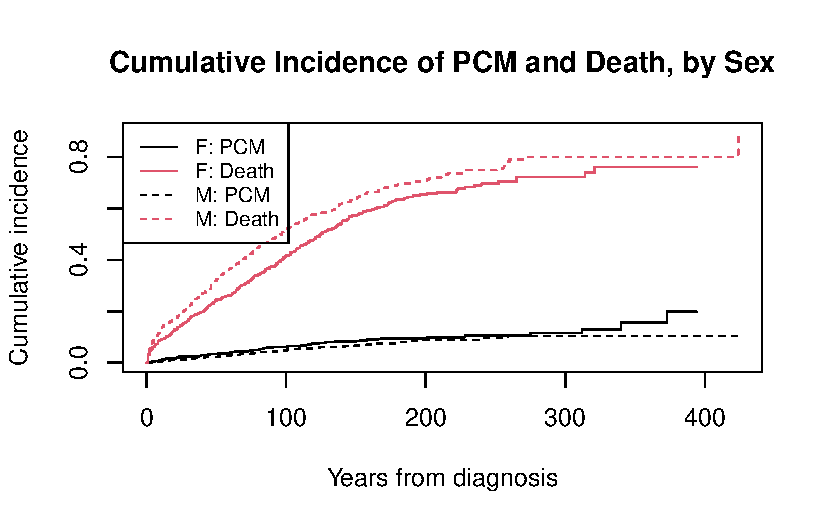
\includegraphics[width=0.85\linewidth,height=\textheight,keepaspectratio]{Section2/Survival analysis/Survival_analysis_files/figure-pdf/unnamed-chunk-19-1.pdf}
\end{center}

When a \texttt{Surv()} object has more than two states (with the first
factor level treated as censoring), \texttt{survfit()} automatically
returns the cumulative incidence for each competing event type rather
than an ordinary KM survival curve --- this is the modern R equivalent
of the Fine-and-Gray cumulative incidence approach.

\subsection{The Lunn-McNeil Alternative (Method
2)}\label{the-lunn-mcneil-alternative-method-2}

An alternative strategy, the \textbf{Lunn-McNeil approach}, duplicates
each subject's data row once per competing risk type and fits a single
\textbf{stratified} Cox model (stratified on event type) to the
augmented data set, rather than fitting separate models for each cause.
With appropriate coding, this reproduces the same hazard ratios as the
cause-specific approach, but additionally allows direct statistical
tests of whether a covariate's effect differs across event types (i.e.,
whether a no-interaction model, with one common coefficient per
covariate across event types, is adequate, versus needing separate
coefficients per event type) --- a comparison that is awkward to make
when the cause-specific models are fit completely separately.

\section{Extensions: Machine Learning Approaches to Survival
Analysis}\label{extensions-machine-learning-approaches-to-survival-analysis}

Beyond the classical toolbox covered in this chapter, a growing set of
machine-learning methods extend survival analysis to high-dimensional
and more flexible settings:

\begin{itemize}
\tightlist
\item
  \textbf{Regularized Cox models} (ridge, LASSO, elastic net via, e.g.,
  the \texttt{glmnet} package) add a penalty to the partial likelihood,
  which stabilizes estimation and performs implicit variable selection
  when the number of predictors is large relative to the number of
  events (common in genomic or high-dimensional EHR data), addressing
  the multicollinearity and overfitting problems of an unpenalized Cox
  model in that setting.
\item
  \textbf{Survival trees} recursively split the covariate space (like a
  classification/regression tree) using a dissimilarity measure ---
  often the log-rank statistic --- to find the split that maximizes the
  survival difference between resulting nodes.
\item
  \textbf{Random survival forests} ensemble many survival trees
  (analogous to random forests for regression/classification) for
  improved prediction accuracy and reduced overfitting.
\item
  \textbf{Deep learning approaches} (e.g., DeepSurv, a deep Cox
  proportional-hazards network) replace the linear predictor
  \(\sum \beta_i X_i\) with a neural network, allowing flexible,
  non-linear modeling of covariate effects on the hazard, and have been
  extended to convolutional architectures (for imaging data), transfer
  learning, and active learning settings for censored data.
\end{itemize}

These methods trade some of the interpretability of the classical Cox
model for greater flexibility and predictive performance, and are an
active area of ongoing methodological research.

\section{Summary of Key R Functions for Survival
Analysis}\label{summary-of-key-r-functions-for-survival-analysis}

\begin{longtable}[]{@{}
  >{\raggedright\arraybackslash}p{(\linewidth - 4\tabcolsep) * \real{0.3333}}
  >{\raggedright\arraybackslash}p{(\linewidth - 4\tabcolsep) * \real{0.3333}}
  >{\raggedright\arraybackslash}p{(\linewidth - 4\tabcolsep) * \real{0.3333}}@{}}
\toprule\noalign{}
\begin{minipage}[b]{\linewidth}\raggedright
Function
\end{minipage} & \begin{minipage}[b]{\linewidth}\raggedright
Package
\end{minipage} & \begin{minipage}[b]{\linewidth}\raggedright
Purpose
\end{minipage} \\
\midrule\noalign{}
\endhead
\bottomrule\noalign{}
\endlastfoot
\texttt{Surv()} & survival & Creates the survival outcome object (time,
status, or start/stop/status) \\
\texttt{survfit()} & survival & Estimates Kaplan-Meier curves; produces
cumulative incidence for multi-state outcomes \\
\texttt{survdiff()} & survival & Performs the log-rank test comparing
survival across groups \\
\texttt{coxph()} & survival & Fits the (semi-parametric) Cox
proportional hazards model, including stratified and time-dependent
(counting-process) extensions \\
\texttt{cox.zph()} & survival & Tests and plots the proportional hazards
assumption via scaled Schoenfeld residuals \\
\texttt{survreg()} & survival & Fits fully parametric survival models
(exponential, Weibull, log-normal, log-logistic AFT models) \\
\texttt{concordance()} & survival & Computes Harrell's (and, with
weighting, Uno's) C-statistic \\
\texttt{p.adjust()} & stats & Adjusts p-values for multiple comparisons
(Bonferroni, BH/FDR, etc.) \\
\end{longtable}

\section{A Complete Worked Example: The NCCTG Lung Cancer
Data}\label{a-complete-worked-example-the-ncctg-lung-cancer-data}

To tie the chapter together, the \texttt{lung} data set (North Central
Cancer Treatment Group, Loprinzi et al.~1994; \(N=228\), 63 censored)
--- already introduced at the start of this chapter --- can be carried
through the full analytic pipeline described above: descriptive KM
curves, a log-rank comparison, a multivariable Cox model, a PH
assumption check, and a parametric alternative.

\begin{Shaded}
\begin{Highlighting}[]
\CommentTok{\# 1. Kaplan{-}Meier by sex, with log{-}rank test}
\NormalTok{km\_sex }\OtherTok{\textless{}{-}} \FunctionTok{survfit}\NormalTok{(}\FunctionTok{Surv}\NormalTok{(time, status) }\SpecialCharTok{\textasciitilde{}}\NormalTok{ sex, }\AttributeTok{data =}\NormalTok{ lung)}
\NormalTok{km\_sex}
\end{Highlighting}
\end{Shaded}

\begin{verbatim}
#> Call: survfit(formula = Surv(time, status) ~ sex, data = lung)
#> 
#>              n events median 0.95LCL 0.95UCL
#> sex=Male   138    112    270     212     310
#> sex=Female  90     53    426     348     550
\end{verbatim}

\begin{Shaded}
\begin{Highlighting}[]
\FunctionTok{survdiff}\NormalTok{(}\FunctionTok{Surv}\NormalTok{(time, status) }\SpecialCharTok{\textasciitilde{}}\NormalTok{ sex, }\AttributeTok{data =}\NormalTok{ lung)}
\end{Highlighting}
\end{Shaded}

\begin{verbatim}
#> Call:
#> survdiff(formula = Surv(time, status) ~ sex, data = lung)
#> 
#>              N Observed Expected (O-E)^2/E (O-E)^2/V
#> sex=Male   138      112     91.6      4.55      10.3
#> sex=Female  90       53     73.4      5.68      10.3
#> 
#>  Chisq= 10.3  on 1 degrees of freedom, p= 0.001
\end{verbatim}

\begin{Shaded}
\begin{Highlighting}[]
\FunctionTok{plot}\NormalTok{(km\_sex, }\AttributeTok{col =} \FunctionTok{c}\NormalTok{(}\StringTok{"blue"}\NormalTok{, }\StringTok{"red"}\NormalTok{), }\AttributeTok{xlab =} \StringTok{"Days"}\NormalTok{, }\AttributeTok{ylab =} \StringTok{"Survival probability"}\NormalTok{,}
     \AttributeTok{main =} \StringTok{"NCCTG Lung Cancer: Survival by Sex"}\NormalTok{)}
\FunctionTok{legend}\NormalTok{(}\StringTok{"topright"}\NormalTok{, }\AttributeTok{legend =} \FunctionTok{c}\NormalTok{(}\StringTok{"Male"}\NormalTok{, }\StringTok{"Female"}\NormalTok{), }\AttributeTok{col =} \FunctionTok{c}\NormalTok{(}\StringTok{"blue"}\NormalTok{, }\StringTok{"red"}\NormalTok{), }\AttributeTok{lty =} \DecValTok{1}\NormalTok{)}
\end{Highlighting}
\end{Shaded}

\begin{center}
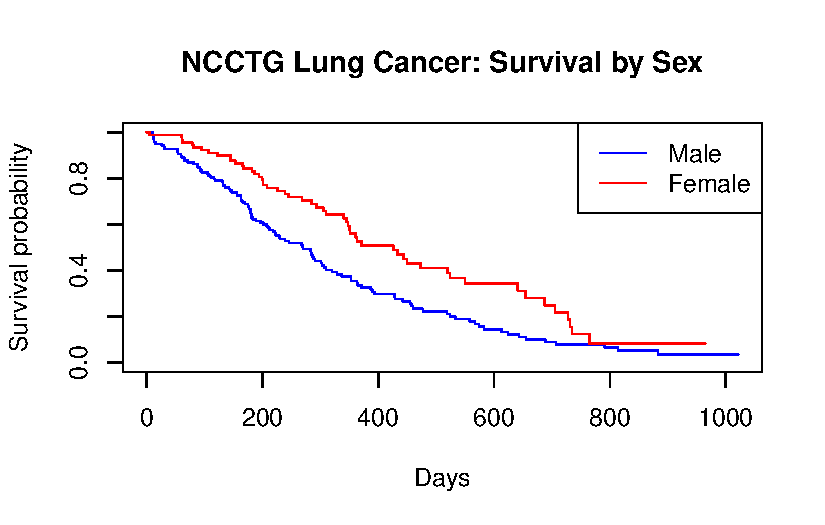
\includegraphics[width=0.85\linewidth,height=\textheight,keepaspectratio]{Section2/Survival analysis/Survival_analysis_files/figure-pdf/unnamed-chunk-20-1.pdf}
\end{center}

\begin{Shaded}
\begin{Highlighting}[]
\CommentTok{\# 2. Multivariable Cox PH model}
\NormalTok{cox\_lung }\OtherTok{\textless{}{-}} \FunctionTok{coxph}\NormalTok{(}\FunctionTok{Surv}\NormalTok{(time, status) }\SpecialCharTok{\textasciitilde{}}\NormalTok{ age }\SpecialCharTok{+}\NormalTok{ sex }\SpecialCharTok{+}\NormalTok{ ph.ecog }\SpecialCharTok{+}\NormalTok{ wt.loss, }\AttributeTok{data =}\NormalTok{ lung)}
\FunctionTok{summary}\NormalTok{(cox\_lung)}
\end{Highlighting}
\end{Shaded}

\begin{verbatim}
#> Call:
#> coxph(formula = Surv(time, status) ~ age + sex + ph.ecog + wt.loss, 
#>     data = lung)
#> 
#>   n= 213, number of events= 151 
#>    (15 observations deleted due to missingness)
#> 
#>                coef exp(coef)  se(coef)      z Pr(>|z|)    
#> age        0.013369  1.013459  0.009628  1.389 0.164951    
#> sexFemale -0.590775  0.553898  0.175339 -3.369 0.000754 ***
#> ph.ecog    0.515111  1.673824  0.125988  4.089 4.34e-05 ***
#> wt.loss   -0.009006  0.991034  0.006658 -1.353 0.176135    
#> ---
#> Signif. codes:  0 '***' 0.001 '**' 0.01 '*' 0.05 '.' 0.1 ' ' 1
#> 
#>           exp(coef) exp(-coef) lower .95 upper .95
#> age          1.0135     0.9867    0.9945    1.0328
#> sexFemale    0.5539     1.8054    0.3928    0.7811
#> ph.ecog      1.6738     0.5974    1.3076    2.1427
#> wt.loss      0.9910     1.0090    0.9782    1.0041
#> 
#> Concordance= 0.647  (se = 0.026 )
#> Likelihood ratio test= 31.02  on 4 df,   p=3e-06
#> Wald test            = 29.94  on 4 df,   p=5e-06
#> Score (logrank) test = 30.65  on 4 df,   p=4e-06
\end{verbatim}

\begin{Shaded}
\begin{Highlighting}[]
\CommentTok{\# 3. Check the PH assumption}
\FunctionTok{cox.zph}\NormalTok{(cox\_lung)}
\end{Highlighting}
\end{Shaded}

\begin{verbatim}
#>          chisq df    p
#> age     0.4353  1 0.51
#> sex     2.6731  1 0.10
#> ph.ecog 1.6355  1 0.20
#> wt.loss 0.0457  1 0.83
#> GLOBAL  4.7516  4 0.31
\end{verbatim}

\begin{Shaded}
\begin{Highlighting}[]
\CommentTok{\# 4. Parametric (Weibull AFT) alternative}
\NormalTok{weib\_lung }\OtherTok{\textless{}{-}} \FunctionTok{survreg}\NormalTok{(}\FunctionTok{Surv}\NormalTok{(time, status) }\SpecialCharTok{\textasciitilde{}}\NormalTok{ age }\SpecialCharTok{+}\NormalTok{ sex }\SpecialCharTok{+}\NormalTok{ ph.ecog }\SpecialCharTok{+}\NormalTok{ wt.loss, }\AttributeTok{data =}\NormalTok{ lung,}
                      \AttributeTok{dist =} \StringTok{"weibull"}\NormalTok{)}
\FunctionTok{summary}\NormalTok{(weib\_lung)}
\end{Highlighting}
\end{Shaded}

\begin{verbatim}
#> 
#> Call:
#> survreg(formula = Surv(time, status) ~ age + sex + ph.ecog + 
#>     wt.loss, data = lung, dist = "weibull")
#>                Value Std. Error     z       p
#> (Intercept)  6.75737    0.43508 15.53 < 2e-16
#> age         -0.00889    0.00688 -1.29   0.196
#> sexFemale    0.41616    0.12698  3.28   0.001
#> ph.ecog     -0.36643    0.09040 -4.05 5.0e-05
#> wt.loss      0.00613    0.00473  1.30   0.194
#> Log(scale)  -0.33381    0.06375 -5.24 1.6e-07
#> 
#> Scale= 0.716 
#> 
#> Weibull distribution
#> Loglik(model)= -1047.5   Loglik(intercept only)= -1062.6
#>  Chisq= 30.14 on 4 degrees of freedom, p= 4.6e-06 
#> Number of Newton-Raphson Iterations: 5 
#> n=213 (15 observations deleted due to missingness)
\end{verbatim}

Across the KM/log-rank, Cox, and parametric analyses, female sex and
better ECOG performance status are consistently associated with longer
survival in this cohort --- illustrating how the different tools in this
chapter (non-parametric, semi-parametric, and fully parametric) are
complementary lenses on the same underlying data, and typically tell a
consistent story when their respective assumptions are reasonably
satisfied.

\section{Chapter Summary}\label{chapter-summary}

This chapter developed survival analysis from first principles through
to modern extensions:

\begin{itemize}
\tightlist
\item
  Time-to-event outcomes require \textbf{specialized methods} because
  they combine a (possibly censored) time component with a binary event
  indicator, information that neither pure time-based methods (t-test,
  ANOVA) nor pure binary methods (logistic regression) can fully exploit
\item
  \textbf{Censoring} --- right, left, and interval --- must be handled
  explicitly, under assumptions of independent, random, non-informative
  censoring
\item
  The \textbf{Kaplan-Meier estimator} provides a non-parametric estimate
  of the survivor function, and the \textbf{log-rank test} compares
  survival between groups
\item
  The \textbf{Cox proportional hazards model} is the workhorse
  regression tool for survival data, estimating hazard ratios while
  leaving the baseline hazard unspecified; its core assumption ---
  proportional hazards --- should always be checked graphically (log-log
  plots) and/or formally (Schoenfeld residuals via \texttt{cox.zph()})
\item
  When PH is violated, the \textbf{stratified Cox model} (for
  categorical variables that can be stratified) and the \textbf{extended
  Cox model} (for variables whose effect changes continuously, or
  abruptly via a Heaviside function, over time) offer principled
  solutions
\item
  \textbf{Parametric survival models} (exponential, Weibull, and other
  AFT models) provide an alternative, fully specified framework, with
  the acceleration factor as an intuitive, time-scale measure of
  association
\item
  Careful attention to \textbf{model building} (interaction,
  confounding, the E-V-W framework), \textbf{study design} (power,
  sample size, cross-over, multiplicity), and \textbf{competing risks}
  rounds out the practical toolkit needed to plan, analyze, and
  correctly interpret time-to-event data
\item
  Modern \textbf{machine learning extensions} (regularized Cox
  regression, survival trees, random survival forests, and deep survival
  networks) extend this classical framework to higher-dimensional and
  more flexible settings
\end{itemize}

\section{References}\label{references-3}

\chapter{Sample Size estimation}\label{sample-size-estimation}

\subsection{\texorpdfstring{\textbf{Introduction}}{Introduction}}\label{introduction-9}

Sample size estimation is a important step in the design of any research
study. It determines how many participants or data points are needed to
draw reliable conclusions from the study. An adequately sized sample
ensures that the study has sufficient power to detect a true effect if
one exists, avoids wastage of resources, and protects against ethical
concerns about using either too many or too few research subjects.

\subsection{Characteristics of Sample}\label{characteristics-of-sample}

\subsection{\texorpdfstring{\textbf{1.
Representative}}{1. Representative}}\label{representative}

A representative sample accurately reflects the demographics, behaviors,
or characteristics of the larger population from which it is drawn. This
characteristic is essential to generalize the findings from the sample
to the population. A sample that is not representative may lead to
biased results if the participants have different characteristics from
the general population.

\textbf{Methods to Achieve Representativeness:}

\begin{itemize}
\item
  \textbf{Random Sampling:} Every member of the population has an equal
  chance of being selected.
\item
  \textbf{Stratified Sampling:} The population is divided into subgroups
  (strata) that are known to exist, and random samples are drawn from
  each stratum.
\item
  \textbf{Cluster Sampling:} Randomly selecting entire clusters or
  groups from a population, where each cluster reflects the
  characteristics of the whole.
\end{itemize}

\subsection{\texorpdfstring{\textbf{2. Sufficiently
Large}}{2. Sufficiently Large}}\label{sufficiently-large}

The sample must be large enough to provide reliable, statistically valid
results. The size needed depends on the expected effect size, the
variability in the data, the desired power of the study (i.e., the
probability of detecting an effect if one exists), and the acceptable
level of type I and type II errors.

\textbf{Benefits of Adequate Sample Size:}

\begin{itemize}
\item
  \textbf{Increased Precision:} Larger samples tend to yield more
  precise estimates of the population parameters.
\item
  \textbf{Reduced Sampling Error:} The error between the sample
  statistic and the population parameter is likely to be smaller.
\end{itemize}

\subsection{\texorpdfstring{\textbf{3.
Efficient}}{3. Efficient}}\label{efficient}

An efficient sample is one that provides the maximum amount of
information needed for the study while using the least amount of
resources (time, money, effort). Efficiency is particularly important in
studies with limited resources or when the study involves hard-to-reach
populations.

\textbf{Strategies for Efficiency:}

\begin{itemize}
\item
  \textbf{Optimal Allocation in Stratified Sampling:} Dividing resources
  in a way that maximizes the variability captured by each part of the
  sample.
\item
  \textbf{Multistage Sampling:} Combining several sampling methods can
  be more resource-efficient than a simple random sample, especially for
  large, geographically dispersed populations.
\end{itemize}

\subsection{\texorpdfstring{\textbf{4. Easy to
Draw}}{4. Easy to Draw}}\label{easy-to-draw}

The sample should be such that it can be drawn without undue difficulty.
This means considering logistical aspects of sampling, such as the ease
of accessing the population, the availability of contact information,
and the willingness of individuals to participate.

\textbf{Considerations for Easy Sampling:}

\begin{itemize}
\item
  \textbf{Accessibility of the Population:} Choosing a population that
  is readily accessible and willing to participate can significantly
  simplify the process of sample collection.
\item
  \textbf{Practicality of Sampling Methods:} Employing sampling methods
  that are practical and feasible under the circumstances of the study,
  like using existing databases or online platforms for surveys when
  face-to-face interaction is not possible.
\end{itemize}

\subsection{How large sample size should
be?}\label{how-large-sample-size-should-be}

Determining the appropriate sample size for a study is crucial because
both excessively small and overly large sample sizes can lead to
significant drawbacks. Let's explore these conditions in more detail:

\subsubsection{\texorpdfstring{\textbf{When the Sample Size is Too
Small}}{When the Sample Size is Too Small}}\label{when-the-sample-size-is-too-small}

\begin{enumerate}
\def\labelenumi{\arabic{enumi}.}
\item
  \textbf{Failure to Detect Clinically Important Associations or
  Differences:} A small sample size has limited statistical power, which
  means the study might not be able to detect significant effects or
  differences that are clinically meaningful. This inability to observe
  a true effect can lead to false negatives (Type II errors).
\item
  \textbf{Imprecise Estimation of Associations or Differences:} With
  fewer data points, the estimates of parameters such as means,
  proportions, or correlations become less precise. This lack of
  precision is reflected in wider confidence intervals, making it
  difficult to draw firm conclusions from the data.
\item
  \textbf{Failure to Answer Research Questions:} If the sample size is
  insufficient to provide clear, reliable results, the primary research
  questions may remain unanswered. This ambiguity can render the
  research inconclusive and, in many cases, necessitates further study,
  delaying potential advancements in the field.
\item
  \textbf{Waste of Participant Input:} Participants who contribute their
  time and information to a study that is too small may feel their
  effort is wasted if the study fails to provide meaningful results.
  This can affect participant morale and willingness to engage in future
  research.
\end{enumerate}

\subsubsection{\texorpdfstring{\textbf{When the Sample Size is Too
Large}}{When the Sample Size is Too Large}}\label{when-the-sample-size-is-too-large}

\begin{enumerate}
\def\labelenumi{\arabic{enumi}.}
\item
  \textbf{Waste of Resources:} Excessively large samples involve more
  logistical arrangements, more staff time, and potentially more
  equipment and materials than are actually needed to achieve the
  objectives of the study.
\item
  \textbf{Waste of Money:} The costs associated with data collection,
  data management, and analysis increase with the size of the sample.
  Over-recruitment can lead to unnecessary expenditure that could have
  been allocated to other important aspects of the study or other
  research projects.
\item
  \textbf{Waste of Time:} Managing a larger sample size often requires
  additional time for data collection, entry, and analysis. This not
  only extends the timeline of the current project but may also delay
  the initiation of subsequent studies.
\item
  \textbf{Difficulty in Maintaining Quality of Data:} As sample sizes
  increase, maintaining consistency and accuracy in data collection
  across many subjects and settings can become challenging. Larger
  datasets can introduce more opportunities for errors in data entry,
  loss of data fidelity, and complications in data management.
\end{enumerate}

Thus sample size should be optimum. Optimum sample size can be
identified through sample size calculation. The importance of sample
size calculation are :

\begin{enumerate}
\def\labelenumi{\arabic{enumi}.}
\tightlist
\item
  Allow appropriate analysis'
\item
  Provide desired level of accuracy
\item
  Allow validity of significance test
\item
  Required for ethical approval
\end{enumerate}

\subsection{\texorpdfstring{\textbf{Fundamentals of Sample Size
Estimation}}{Fundamentals of Sample Size Estimation}}\label{fundamentals-of-sample-size-estimation}

\subsubsection{\texorpdfstring{\textbf{1. Objective of the
Study}}{1. Objective of the Study}}\label{objective-of-the-study}

The purpose of the study heavily influences sample size. Objectives can
vary from estimating a parameter (like an average or proportion) with a
specified precision, to detecting a difference between groups, or to
establishing a correlation between variables.

\subsubsection{\texorpdfstring{\textbf{2. Significance Level
(α)}}{2. Significance Level (α)}}\label{significance-level-ux3b1}

The significance level is the probability of rejecting the null
hypothesis when it is actually true (Type I error). A common value used
is 0.05, implying a 5\% risk of a Type I error.

\subsubsection{\texorpdfstring{\textbf{3. Power (1 -
β)}}{3. Power (1 - β)}}\label{power-1---ux3b2}

Power is the probability of correctly rejecting the null hypothesis when
it is false, essentially avoiding a Type II error. A typical power used
in studies is 80\% or 90\%, depending on the importance of the outcome
being studied.

\subsubsection{\texorpdfstring{\textbf{4. Effect
Size}}{4. Effect Size}}\label{effect-size}

Effect size is a quantitative measure of the magnitude of the
experimental effect that the researcher seeks to detect. The larger the
effect size, the smaller the sample size required to detect it.

Sample size calculation for different scenarios

\section{Sample size calculation for Cross-section study estimating
simple
prevalence}\label{sample-size-calculation-for-cross-section-study-estimating-simple-prevalence}

\subsection{Using precision based
approach}\label{using-precision-based-approach}

\subsubsection{When population is finite and anticipated population
proportion is not
known.}\label{when-population-is-finite-and-anticipated-population-proportion-is-not-known.}

In this scenario, we can use Yamane formula

\[ n = \frac{1}{1 + N.d^2} \] where N is total count of finite
population and d is the absolute error

Lets create a function to calculate sample size by Yamane formula

\begin{Shaded}
\begin{Highlighting}[]
\CommentTok{\# lets generate a function for yamane formula}
\NormalTok{yamane}\OtherTok{\textless{}{-}}\ControlFlowTok{function}\NormalTok{(N, abs.err)\{}
\NormalTok{  n}\OtherTok{=}\NormalTok{N}\SpecialCharTok{/}\NormalTok{(}\DecValTok{1}\SpecialCharTok{+}\NormalTok{N}\SpecialCharTok{*}\NormalTok{abs.err}\SpecialCharTok{\^{}}\DecValTok{2}\NormalTok{)}
  \FunctionTok{cat}\NormalTok{(}\StringTok{"Sample size is :"}\NormalTok{, }\StringTok{"}\SpecialCharTok{\textbackslash{}n}\StringTok{"}\NormalTok{, }\FunctionTok{ceiling}\NormalTok{(n))}
\NormalTok{\}}
\end{Highlighting}
\end{Shaded}

\textbf{Example:} Let us consider, you are interested in carrying a
prevalence study using simple random sampling from a population of over
12000 university students. There were no previous studies to anticipate
prevalence. What is the required sample size to estimate prevalence
within 5\% point of the true prevalence.

\textbf{Solution:}

Here, N=12000; d=0.05

\begin{Shaded}
\begin{Highlighting}[]
\CommentTok{\# Calculate sample size using our own function}
\FunctionTok{yamane}\NormalTok{(}\DecValTok{12000}\NormalTok{, }\FloatTok{0.05}\NormalTok{)}
\end{Highlighting}
\end{Shaded}

\begin{verbatim}
#> Sample size is : 
#>  388
\end{verbatim}

\subsubsection{When anticipated population proportion is known and
population is not
finite.}\label{when-anticipated-population-proportion-is-known-and-population-is-not-finite.}

To calculate sample size for this scenario, we require anticipated
population proportion (p), confidence level (1-alpha) and absolute
precision (d). The required formula is chchrane formula as follow:

\[ n = \frac{Z^2. p(1-p)}{d^2} \] where Z=1.96 at 95\% confidence level,
p=anticipated population proportion and d is absolute precision.

To calculated sample size for this situation, we can use
\texttt{epi.sssimpleestb()} function from \texttt{epiR} package or we
can use the following function.

\begin{Shaded}
\begin{Highlighting}[]
\CommentTok{\# Lets generate our own function to calculate sample size when anticipated population proportion is known and population is not finite}

\NormalTok{sscal\_oneprop\_precision\_based}\OtherTok{\textless{}{-}}\ControlFlowTok{function}\NormalTok{(P, error, }\AttributeTok{error\_type=}\FunctionTok{c}\NormalTok{(}\StringTok{"absolute"}\NormalTok{, }\StringTok{"relative"}\NormalTok{), }\AttributeTok{conf.int=}\FloatTok{0.95}\NormalTok{, }\AttributeTok{N=}\ConstantTok{NA}\NormalTok{)\{}
\NormalTok{  alpha}\OtherTok{=}\DecValTok{1}\SpecialCharTok{{-}}\NormalTok{conf.int}
\NormalTok{  Za}\OtherTok{=}\FunctionTok{qnorm}\NormalTok{(}\AttributeTok{p=}\DecValTok{1}\SpecialCharTok{{-}}\NormalTok{alpha}\SpecialCharTok{/}\DecValTok{2}\NormalTok{, }\AttributeTok{mean=}\DecValTok{0}\NormalTok{, }\AttributeTok{sd=}\DecValTok{1}\NormalTok{)}
  \ControlFlowTok{if}\NormalTok{(error\_type}\SpecialCharTok{==}\StringTok{"relative"}\NormalTok{)\{}
\NormalTok{  n}\OtherTok{=}\NormalTok{Za}\SpecialCharTok{\^{}}\DecValTok{2}\SpecialCharTok{*}\NormalTok{(}\DecValTok{1}\SpecialCharTok{{-}}\NormalTok{P)}\SpecialCharTok{/}\NormalTok{(P}\SpecialCharTok{*}\NormalTok{error}\SpecialCharTok{\^{}}\DecValTok{2}\NormalTok{)}
\NormalTok{  n }\OtherTok{\textless{}{-}} \FunctionTok{ifelse}\NormalTok{(}\FunctionTok{is.na}\NormalTok{(N), n, (n }\SpecialCharTok{*}\NormalTok{ N)}\SpecialCharTok{/}\NormalTok{(n }\SpecialCharTok{+}\NormalTok{ (N }\SpecialCharTok{{-}} \DecValTok{1}\NormalTok{)))}
\NormalTok{  \}}
  \ControlFlowTok{else}\NormalTok{\{}
\NormalTok{    n}\OtherTok{=}\NormalTok{Za}\SpecialCharTok{\^{}}\DecValTok{2}\SpecialCharTok{*}\NormalTok{(P}\SpecialCharTok{*}\NormalTok{(}\DecValTok{1}\SpecialCharTok{{-}}\NormalTok{P)}\SpecialCharTok{/}\NormalTok{error}\SpecialCharTok{\^{}}\DecValTok{2}\NormalTok{)}
\NormalTok{    n }\OtherTok{\textless{}{-}} \FunctionTok{ifelse}\NormalTok{(}\FunctionTok{is.na}\NormalTok{(N), n, (n }\SpecialCharTok{*}\NormalTok{ N)}\SpecialCharTok{/}\NormalTok{(n }\SpecialCharTok{+}\NormalTok{ (N }\SpecialCharTok{{-}} \DecValTok{1}\NormalTok{)))}
\NormalTok{    \}}
  
  \FunctionTok{cat}\NormalTok{(}\StringTok{"Sample size is:"}\NormalTok{, }\StringTok{"}\SpecialCharTok{\textbackslash{}n}\StringTok{"}\NormalTok{, }\FunctionTok{ceiling}\NormalTok{(n))}
\NormalTok{\}}
\end{Highlighting}
\end{Shaded}

\textbf{Example:} Let us consider, we wanted to calculate prevalence of
hepatitis among adults age 15-49 years old. How many adults should be
included in the study so that the estimated prevalence is within 2\%
point of the true value with 95\% confidence level and it is estimated
from the previous study that prevalence is 10\%.

\textbf{Solution:}

Here, p=10\%; 1-alpha =95\%; d=2\%

\begin{Shaded}
\begin{Highlighting}[]
\CommentTok{\# install.packages("epiR")}
\FunctionTok{library}\NormalTok{(epiR)}

\CommentTok{\# Error: package or namespace load failed for ‘epiR’ in loadNamespace(j \textless{}{-} i[[1L]], c(lib.loc, .libPaths()), versionCheck = vI[[j]]):}
\CommentTok{\#  there is no package called ‘gfonts’}
\CommentTok{\# In addition: Warning message:}
\CommentTok{\# package ‘epiR’ was built under R version 4.4.2}

\CommentTok{\# I got error due to absenence of \textquotesingle{}gfonts\textquotesingle{} so i\textquotesingle{}m installing it.}

\CommentTok{\# install.packages(\textquotesingle{}gfonts\textquotesingle{})}

\CommentTok{\# use epi.sssimpleestb() function from epiR package}
\FunctionTok{epi.sssimpleestb}\NormalTok{(}\AttributeTok{Py =} \FloatTok{0.10}\NormalTok{, }\AttributeTok{epsilon =} \FloatTok{0.02}\NormalTok{,}\AttributeTok{error =} \StringTok{"absolute"}\NormalTok{,}\AttributeTok{conf.level =} \FloatTok{0.95}\NormalTok{, }\AttributeTok{se =}\DecValTok{1}\NormalTok{, }\AttributeTok{sp =} \DecValTok{1}\NormalTok{)}
\end{Highlighting}
\end{Shaded}

\begin{verbatim}
#> [1] 865
\end{verbatim}

\begin{Shaded}
\begin{Highlighting}[]
\CommentTok{\# using created function}
\FunctionTok{sscal\_oneprop\_precision\_based}\NormalTok{(}\AttributeTok{P =} \FloatTok{0.10}\NormalTok{, }\AttributeTok{error =} \FloatTok{0.02}\NormalTok{, }\AttributeTok{error\_type =} \StringTok{"absolute"}\NormalTok{, }\AttributeTok{conf.int =} \FloatTok{0.95}\NormalTok{)}
\end{Highlighting}
\end{Shaded}

\begin{verbatim}
#> Sample size is: 
#>  865
\end{verbatim}

\subsubsection{When anticipated population proportion is known and
population is
finite}\label{when-anticipated-population-proportion-is-known-and-population-is-finite}

When population is finite, we have to correct our sample size which can
be carried out by using following formula

\[ n = \frac{n_0.N}{n_0 +(N-1)} \] where n0 is the calculated sample
size from the previous formula.

We can calculate sample size using \texttt{epi.sssimpleestb()} from epiR
package or function created before.

\textbf{Example:} Let us consider, we wanted to calculate prevalence of
hepatitis among adults age 15-49 years old in the hotel of population
1500. How many adults should be included in the study so that the
estimated prevalence is within 20\% relative error and 95\% confidence
level and it is estimated from the previous study that prevalence is
10\%.

\textbf{Solution:}

p=10\%; 1-alpha =95\%; d=2\%; N=1500

Now lets calculate sample size using R

\begin{Shaded}
\begin{Highlighting}[]
\CommentTok{\# Using epiR package}
\FunctionTok{epi.sssimpleestb}\NormalTok{(}\AttributeTok{Py =} \FloatTok{0.10}\NormalTok{, }\AttributeTok{epsilon =} \FloatTok{0.2}\NormalTok{,}\AttributeTok{error =} \StringTok{"relative"}\NormalTok{,}\AttributeTok{conf.level =} \FloatTok{0.95}\NormalTok{, }\AttributeTok{se =}\DecValTok{1}\NormalTok{, }\AttributeTok{sp =} \DecValTok{1}\NormalTok{, }\AttributeTok{N =} \DecValTok{1500}\NormalTok{)}
\end{Highlighting}
\end{Shaded}

\begin{verbatim}
#> [1] 549
\end{verbatim}

\begin{Shaded}
\begin{Highlighting}[]
\CommentTok{\# using own function}
\FunctionTok{sscal\_oneprop\_precision\_based}\NormalTok{(}\AttributeTok{P =} \FloatTok{0.10}\NormalTok{, }\AttributeTok{error =} \FloatTok{0.2}\NormalTok{, }\AttributeTok{error\_type =} \StringTok{"relative"}\NormalTok{, }\AttributeTok{conf.int =} \FloatTok{0.95}\NormalTok{, }\AttributeTok{N=}\DecValTok{1500}\NormalTok{)}
\end{Highlighting}
\end{Shaded}

\begin{verbatim}
#> Sample size is: 
#>  549
\end{verbatim}

\subsection{Using power based
approach)}\label{using-power-based-approach}

When studies are designed to test hypothesis that the anticipated
prevalence of condition is less than, greater than or equal to the
hypothesized value. To calculate prevalence through this approach, we
require prevalence under null hypothesis , test prevalence, level of
significance, power of the test and type of alternative hypothesis
(one-sided or both sided).

\subsubsection{One Sample proportion with hypothesis
testing}\label{one-sample-proportion-with-hypothesis-testing}

For the study conducting asymptotic z-test for a single proportion (one
sample test), the sample size can be calculated using the formula that
uses normal approximation to the distribution of the test statistic. The
formula is as follow:

\[
n=\frac{\left( Z_a \sqrt{P_0 (1 - P_0)} + Z_b \sqrt{P (1 - P)} \right)^2}{(P_0 - P)^2}
\]

where,

P0 is population proportion under null hypothesis

Pa is anticipated value of the population proportion (proportion under
alternative hypothesis)

Za is Z value at x\% CI (one sided or two sided)

Zb is Z value at y\% power

\begin{Shaded}
\begin{Highlighting}[]
\CommentTok{\# Function}
\NormalTok{sscal\_oneprop\_power\_based}\OtherTok{\textless{}{-}}\ControlFlowTok{function}\NormalTok{(P0, P, }\AttributeTok{sided.test=}\FunctionTok{c}\NormalTok{(}\StringTok{"one sided"}\NormalTok{, }\StringTok{"two sided"}\NormalTok{), }\AttributeTok{conf.int=}\FloatTok{0.95}\NormalTok{, }\AttributeTok{power=}\FloatTok{0.80}\NormalTok{)\{}
\NormalTok{  alpha}\OtherTok{=}\DecValTok{1}\SpecialCharTok{{-}}\NormalTok{conf.int}
  \ControlFlowTok{if}\NormalTok{(sided.test}\SpecialCharTok{==}\StringTok{"two sided"}\NormalTok{)\{}
\NormalTok{  Za}\OtherTok{=}\FunctionTok{qnorm}\NormalTok{(}\AttributeTok{p=}\DecValTok{1}\SpecialCharTok{{-}}\NormalTok{alpha}\SpecialCharTok{/}\DecValTok{2}\NormalTok{, }\AttributeTok{mean=}\DecValTok{0}\NormalTok{, }\AttributeTok{sd=}\DecValTok{1}\NormalTok{)}
\NormalTok{  \} }\ControlFlowTok{else}\NormalTok{\{Za}\OtherTok{=}\FunctionTok{qnorm}\NormalTok{(}\AttributeTok{p=}\DecValTok{1}\SpecialCharTok{{-}}\NormalTok{alpha, }\AttributeTok{mean=}\DecValTok{0}\NormalTok{, }\AttributeTok{sd=}\DecValTok{1}\NormalTok{)\}}
  
\NormalTok{  beta}\OtherTok{=}\DecValTok{1}\SpecialCharTok{{-}}\NormalTok{power}
\NormalTok{  Zb}\OtherTok{=}\FunctionTok{qnorm}\NormalTok{(}\AttributeTok{p=}\DecValTok{1}\SpecialCharTok{{-}}\NormalTok{beta, }\AttributeTok{mean=}\DecValTok{0}\NormalTok{, }\AttributeTok{sd=}\DecValTok{1}\NormalTok{)}
  
\NormalTok{  n}\OtherTok{=}\NormalTok{(\{Za}\SpecialCharTok{*}\FunctionTok{sqrt}\NormalTok{(P0}\SpecialCharTok{*}\NormalTok{(}\DecValTok{1}\SpecialCharTok{{-}}\NormalTok{P0))}\SpecialCharTok{+}\NormalTok{Zb}\SpecialCharTok{*}\FunctionTok{sqrt}\NormalTok{(P}\SpecialCharTok{*}\NormalTok{(}\DecValTok{1}\SpecialCharTok{{-}}\NormalTok{P))\}}\SpecialCharTok{\^{}}\DecValTok{2}\NormalTok{)}\SpecialCharTok{/}\NormalTok{(P0}\SpecialCharTok{{-}}\NormalTok{P)}\SpecialCharTok{\^{}}\DecValTok{2}
  
  \FunctionTok{cat}\NormalTok{(}\StringTok{"Sample size is:"}\NormalTok{, }\StringTok{"}\SpecialCharTok{\textbackslash{}n}\StringTok{"}\NormalTok{, }\FunctionTok{ceiling}\NormalTok{(n))}
\NormalTok{\}}

\CommentTok{\# Calculation}
\FunctionTok{sscal\_oneprop\_power\_based}\NormalTok{(}\AttributeTok{P0 =}\FloatTok{0.25}\NormalTok{, }\AttributeTok{P =} \FloatTok{0.2}\NormalTok{,}\AttributeTok{sided.test =} \StringTok{"two sided"}\NormalTok{, }\AttributeTok{power =} \FloatTok{0.9}\NormalTok{,}\AttributeTok{conf.int =} \FloatTok{0.95}\NormalTok{ )}
\end{Highlighting}
\end{Shaded}

\begin{verbatim}
#> Sample size is: 
#>  742
\end{verbatim}

\textbf{Example:} The success rate for a surgical treatment of a
particular heart condition is widely reported in the literature to be
70\%. A new medical treatment has been proposed that is alleged to offer
equivalent treatment success. A hospital without the necessary
facilities or staff to provide the surgical treatment has decided to use
the new medical treatment for all new patients presenting with this
condition. How many patients must be studied to test the hypothesis that
the success rate of the new method of treatment is 70\% against an
alternative hypothesis that it is not 70\% at the 5\% level of
significance? The investigators wish to have a 90\% power of detecting a
difference between the success rates of 10 percentage points or more in
either direction.

\textbf{Solution:}

test success rate (p0)= 0.7

anticipated success rate (p)=0.8 or 0.6

alpha=0.05

power =0.9

sided test = two sided

\begin{Shaded}
\begin{Highlighting}[]
\CommentTok{\# install.packages("pwrss")}
\FunctionTok{library}\NormalTok{(pwrss)}

\FunctionTok{pwrss.z.prop}\NormalTok{(}\AttributeTok{p =} \FloatTok{0.8}\NormalTok{, }\AttributeTok{p0 =} \FloatTok{0.7}\NormalTok{, }\AttributeTok{alpha =} \FloatTok{0.05}\NormalTok{, }\AttributeTok{power =} \FloatTok{0.90}\NormalTok{,}
\NormalTok{      ,}
             \AttributeTok{arcsin.trans =} \ConstantTok{FALSE}\NormalTok{)}
\end{Highlighting}
\end{Shaded}

\begin{verbatim}
#> +--------------------------------------------------+
#> |             SAMPLE SIZE CALCULATION              |
#> +--------------------------------------------------+
#> 
#> One Proportion
#> 
#>   Method                 : Normal Approximation
#>   Continuity Correction  : FALSE
#>   Arcsine Transformation : FALSE
#>   Standard Error         : Calculated From Null
#> 
#> ----------------------------------------------------
#> Hypotheses
#> ----------------------------------------------------
#>   H0 (Null)        : prob  = null.prob
#>   H1 (Alternative) : prob != null.prob
#> 
#> ----------------------------------------------------
#> Results
#> ----------------------------------------------------
#>   Target Effect (prob) = 0.800 (vs. null.prob = 0.700)
#>   Sample Size          = 200  <<
#>   Type 1 Error (alpha) = 0.050
#>   Type 2 Error (beta)  = 0.099
#>   Statistical Power    = 0.901
\end{verbatim}

\section{Sample size calculation for study estimating difference in two
proportions}\label{sample-size-calculation-for-study-estimating-difference-in-two-proportions}

This can be done by two approach:

a) precision based approach

b) power based approach

\subsection{Using precision based
approach}\label{using-precision-based-approach-1}

In this approach, we required anticipated population proportions for two
groups, confidence level, precision level. The formula to calculate
sample size is as follows: \[
n= \frac{Z_a^2 *V^2}{d^2}
\]

Where\\
\[
V=P_1 *(1-P_1)+P_2*(1-P_2)
\]

\textbf{Example:} What sample size should be selected from each of two
groups in order to estimate the risk difference within 5 percentage
points of the true difference, with 95\% confidence, when no reliable
estimates of P1 and P2 are available?

\textbf{Solution:}

precision = 5\% (0.05)

P1, P2 are unknown so lets take 50\% each

confidence level =95\%

\begin{Shaded}
\begin{Highlighting}[]
\CommentTok{\# Using own function}
\NormalTok{sscal\_twoprop\_precision\_based}\OtherTok{\textless{}{-}}\ControlFlowTok{function}\NormalTok{(P1, P2, abs.error, }\AttributeTok{conf.int=}\FloatTok{0.95}\NormalTok{, }\AttributeTok{N=}\ConstantTok{NA}\NormalTok{)\{}
\NormalTok{  alpha}\OtherTok{=}\DecValTok{1}\SpecialCharTok{{-}}\NormalTok{conf.int}
\NormalTok{  Za}\OtherTok{=}\FunctionTok{qnorm}\NormalTok{(}\AttributeTok{p=}\DecValTok{1}\SpecialCharTok{{-}}\NormalTok{alpha}\SpecialCharTok{/}\DecValTok{2}\NormalTok{, }\AttributeTok{mean=}\DecValTok{0}\NormalTok{, }\AttributeTok{sd=}\DecValTok{1}\NormalTok{)}
  
\NormalTok{  V}\OtherTok{=}\NormalTok{P1}\SpecialCharTok{*}\NormalTok{(}\DecValTok{1}\SpecialCharTok{{-}}\NormalTok{P1)}\SpecialCharTok{+}\NormalTok{P2}\SpecialCharTok{*}\NormalTok{(}\DecValTok{1}\SpecialCharTok{{-}}\NormalTok{P2)}
  
\NormalTok{  n}\OtherTok{=}\NormalTok{Za}\SpecialCharTok{\^{}}\DecValTok{2}\SpecialCharTok{*}\NormalTok{V}\SpecialCharTok{/}\NormalTok{(abs.error}\SpecialCharTok{\^{}}\DecValTok{2}\NormalTok{)}
  
  \FunctionTok{cat}\NormalTok{(}\StringTok{"Sample size required }\SpecialCharTok{\textbackslash{}n}\StringTok{ group1: "}\NormalTok{, }\FunctionTok{ceiling}\NormalTok{(n), }\StringTok{"}\SpecialCharTok{\textbackslash{}n}\StringTok{"}\NormalTok{, }\StringTok{"group2:"}\NormalTok{, }\FunctionTok{ceiling}\NormalTok{(n))}
\NormalTok{\}}


\FunctionTok{sscal\_twoprop\_precision\_based}\NormalTok{(}\AttributeTok{P1 =} \FloatTok{0.5}\NormalTok{, }\AttributeTok{P2 =} \FloatTok{0.5}\NormalTok{,}\AttributeTok{abs.error =} \FloatTok{0.05}\NormalTok{,}\AttributeTok{conf.int =} \FloatTok{0.95}\NormalTok{)}
\end{Highlighting}
\end{Shaded}

\begin{verbatim}
#> Sample size required 
#>  group1:  769 
#>  group2: 769
\end{verbatim}

\subsection{Using power based
approach}\label{using-power-based-approach-1}

In power based approach, we required anticipated population proportions
(p1 and p2) , level of significance, power of test and type of test (one
sided or two sided).

\textbf{Example:} An investigator wants to compare the complication
rates between two types of surgery: one with a 15\% complication rate
and the other with a 25\% complication rate. How large should the sample
size be in each group to detect, with 80\% power and a significance
level of 5\%, whether the complication rate of the second surgery is
significantly higher than that of the first?

\textbf{Solution:}

complication rate for the one group (p1)=5\%

complication rate for the another group (p2)=15\%

power: 90\%

Confidence level=95\%

sided test= one sided

\begin{Shaded}
\begin{Highlighting}[]
\NormalTok{sscal\_twoprop\_power\_based}\OtherTok{\textless{}{-}}\ControlFlowTok{function}\NormalTok{(P1, P2, }\AttributeTok{sided.test=}\FunctionTok{c}\NormalTok{(}\StringTok{"one.sided"}\NormalTok{, }\StringTok{"two.sided"}\NormalTok{), }\AttributeTok{conf.int=}\FloatTok{0.95}\NormalTok{, }\AttributeTok{power=}\FloatTok{0.80}\NormalTok{)\{}
\NormalTok{  P}\OtherTok{=}\NormalTok{(P1}\SpecialCharTok{+}\NormalTok{P2)}\SpecialCharTok{/}\DecValTok{2}
\NormalTok{  alpha}\OtherTok{=}\DecValTok{1}\SpecialCharTok{{-}}\NormalTok{conf.int}
  \ControlFlowTok{if}\NormalTok{(sided.test}\SpecialCharTok{==}\StringTok{"two.sided"}\NormalTok{)\{}
\NormalTok{  Za}\OtherTok{=}\FunctionTok{qnorm}\NormalTok{(}\AttributeTok{p=}\DecValTok{1}\SpecialCharTok{{-}}\NormalTok{alpha}\SpecialCharTok{/}\DecValTok{2}\NormalTok{, }\AttributeTok{mean=}\DecValTok{0}\NormalTok{, }\AttributeTok{sd=}\DecValTok{1}\NormalTok{)}
\NormalTok{  \} }\ControlFlowTok{else}\NormalTok{\{Za}\OtherTok{=}\FunctionTok{qnorm}\NormalTok{(}\AttributeTok{p=}\DecValTok{1}\SpecialCharTok{{-}}\NormalTok{alpha, }\AttributeTok{mean=}\DecValTok{0}\NormalTok{, }\AttributeTok{sd=}\DecValTok{1}\NormalTok{)\}}
  
\NormalTok{  beta}\OtherTok{=}\DecValTok{1}\SpecialCharTok{{-}}\NormalTok{power}
\NormalTok{  Zb}\OtherTok{=}\FunctionTok{qnorm}\NormalTok{(}\AttributeTok{p=}\DecValTok{1}\SpecialCharTok{{-}}\NormalTok{beta, }\AttributeTok{mean=}\DecValTok{0}\NormalTok{, }\AttributeTok{sd=}\DecValTok{1}\NormalTok{)}
  
\NormalTok{  n}\OtherTok{=}\NormalTok{(\{Za}\SpecialCharTok{*}\FunctionTok{sqrt}\NormalTok{(}\DecValTok{2}\SpecialCharTok{*}\NormalTok{P}\SpecialCharTok{*}\NormalTok{(}\DecValTok{1}\SpecialCharTok{{-}}\NormalTok{P))}\SpecialCharTok{+}\NormalTok{Zb}\SpecialCharTok{*}\FunctionTok{sqrt}\NormalTok{(P1}\SpecialCharTok{*}\NormalTok{(}\DecValTok{1}\SpecialCharTok{{-}}\NormalTok{P1)}\SpecialCharTok{+}\NormalTok{P2}\SpecialCharTok{*}\NormalTok{(}\DecValTok{1}\SpecialCharTok{{-}}\NormalTok{P2))\}}\SpecialCharTok{\^{}}\DecValTok{2}\NormalTok{)}\SpecialCharTok{/}\NormalTok{(P1}\SpecialCharTok{{-}}\NormalTok{P2)}\SpecialCharTok{\^{}}\DecValTok{2}
  
  \FunctionTok{cat}\NormalTok{(}\StringTok{"Sample size required }\SpecialCharTok{\textbackslash{}n}\StringTok{ group1: "}\NormalTok{, }\FunctionTok{ceiling}\NormalTok{(n), }\StringTok{"}\SpecialCharTok{\textbackslash{}n}\StringTok{"}\NormalTok{, }\StringTok{"group2:"}\NormalTok{, }\FunctionTok{ceiling}\NormalTok{(n))}
\NormalTok{\}}

\CommentTok{\# Calculation}
\FunctionTok{sscal\_twoprop\_power\_based}\NormalTok{(}\AttributeTok{P1 =}\FloatTok{0.15}\NormalTok{, }\AttributeTok{P2 =} \FloatTok{0.25}\NormalTok{,}\AttributeTok{sided.test =} \StringTok{"one.sided"}\NormalTok{, }\AttributeTok{power =} \FloatTok{0.8}\NormalTok{,}\AttributeTok{conf.int =} \FloatTok{0.95}\NormalTok{ )}
\end{Highlighting}
\end{Shaded}

\begin{verbatim}
#> Sample size required 
#>  group1:  197 
#>  group2: 197
\end{verbatim}

\begin{Shaded}
\begin{Highlighting}[]
\CommentTok{\# function from package }
\FunctionTok{power.prop.test}\NormalTok{(}\AttributeTok{p1 =} \FloatTok{0.15}\NormalTok{, }\AttributeTok{p2 =} \FloatTok{0.25}\NormalTok{, }\AttributeTok{sig.level =} \FloatTok{0.05}\NormalTok{, }\AttributeTok{power =} \FloatTok{0.8}\NormalTok{,}\AttributeTok{alternative =} \StringTok{"one.sided"}\NormalTok{)}
\end{Highlighting}
\end{Shaded}

\begin{verbatim}
#> 
#>      Two-sample comparison of proportions power calculation 
#> 
#>               n = 196.7928
#>              p1 = 0.15
#>              p2 = 0.25
#>       sig.level = 0.05
#>           power = 0.8
#>     alternative = one.sided
#> 
#> NOTE: n is number in *each* group
\end{verbatim}

Thus, Th

\section{Sample size calculation for study estimating single group
mean}\label{sample-size-calculation-for-study-estimating-single-group-mean}

\subsection{Using precision based
approach}\label{using-precision-based-approach-2}

Formula:

\[
n=\frac{Z_{\alpha/2}* s^2}{d^2}
\]

where

s is standard deviation obtained from the previous study or pilot study

d is the estimated absolute margin of error

Zα/2 is the normal deviate for 2-tailed test

\begin{Shaded}
\begin{Highlighting}[]
\CommentTok{\# function from package}
\NormalTok{epiR}\SpecialCharTok{::}\FunctionTok{epi.sssimpleestc}\NormalTok{(}\AttributeTok{sigma =} \FloatTok{0.2}\NormalTok{,}\AttributeTok{epsilon =} \FloatTok{0.02}\NormalTok{,}\AttributeTok{error =} \StringTok{"absolute"}\NormalTok{,}\AttributeTok{xbar =} \DecValTok{2}\NormalTok{)}
\end{Highlighting}
\end{Shaded}

\begin{verbatim}
#> [1] 385
\end{verbatim}

\begin{Shaded}
\begin{Highlighting}[]
\CommentTok{\# own function}
\NormalTok{sscal\_onemean\_precision\_based}\OtherTok{\textless{}{-}}\ControlFlowTok{function}\NormalTok{(mean,sd, err, }\AttributeTok{err.type=}\FunctionTok{c}\NormalTok{(}\StringTok{"asolute"}\NormalTok{, }\StringTok{"relative"}\NormalTok{), }\AttributeTok{conf.int=}\FloatTok{0.95}\NormalTok{)\{}
\NormalTok{  alpha}\OtherTok{=}\DecValTok{1}\SpecialCharTok{{-}}\NormalTok{conf.int}
\NormalTok{  Za}\OtherTok{=}\FunctionTok{qnorm}\NormalTok{(}\AttributeTok{p=}\DecValTok{1}\SpecialCharTok{{-}}\NormalTok{alpha}\SpecialCharTok{/}\DecValTok{2}\NormalTok{, }\AttributeTok{mean=}\DecValTok{0}\NormalTok{, }\AttributeTok{sd=}\DecValTok{1}\NormalTok{)}
  
  \ControlFlowTok{if}\NormalTok{(err.type}\SpecialCharTok{==}\StringTok{"absolute"}\NormalTok{)\{}
\NormalTok{   error}\OtherTok{=}\NormalTok{err}
\NormalTok{  \} }\ControlFlowTok{else}\NormalTok{\{}
\NormalTok{   error}\OtherTok{=}\NormalTok{err}\SpecialCharTok{*}\NormalTok{mean}
\NormalTok{  \}}
  
\NormalTok{  n}\OtherTok{=}\NormalTok{(\{Za}\SpecialCharTok{*}\NormalTok{sd\}}\SpecialCharTok{\^{}}\DecValTok{2}\NormalTok{)}\SpecialCharTok{/}\NormalTok{(error)}\SpecialCharTok{\^{}}\DecValTok{2}
  
  \FunctionTok{cat}\NormalTok{(}\StringTok{"Sample size is:"}\NormalTok{, }\StringTok{"}\SpecialCharTok{\textbackslash{}n}\StringTok{"}\NormalTok{, }\FunctionTok{ceiling}\NormalTok{(n))}
\NormalTok{\}}

\FunctionTok{sscal\_onemean\_precision\_based}\NormalTok{(}\AttributeTok{mean =} \DecValTok{1500} \SpecialCharTok{*} \FloatTok{0.05}\NormalTok{,}\AttributeTok{sd =}\NormalTok{(}\DecValTok{300} \SpecialCharTok{*} \FloatTok{0.05}\NormalTok{),}\AttributeTok{err =} \FloatTok{0.20}\NormalTok{, }\AttributeTok{err.type =} \StringTok{"absolute"}\NormalTok{,}\AttributeTok{conf.int =} \FloatTok{0.95}\NormalTok{ )}
\end{Highlighting}
\end{Shaded}

\begin{verbatim}
#> Sample size is: 
#>  21609
\end{verbatim}

\subsection{}\label{section-2}

\section{Sample size calculation for two independent mean
situation}\label{sample-size-calculation-for-two-independent-mean-situation}

The formula to calculate sample size are taken from the Book of
Bernard{[}(\textbf{rosner2011?}). The formula to caculate sample size in
two groups are not equal (r\textgreater1) is as follows:

\[n1=\frac{(\sigma_1^2+\frac{\sigma_2^2}{r})(Z_{\alpha/2}+Z_\beta)^2* \sigma}{(u_1-u_2)}
\]

\[n2=\frac{(r*\sigma_1^2+\sigma_2^2)*(Z_{\alpha/2}+Z_\beta)^2}{(u_1-u_2)^2}
\]

The formula to caculate sample size in two groups are equal (r=1) is as
follows:

\[n=\frac{(\sigma_1^2+\sigma_2^2)*(Z_{\alpha/2}+Z_\beta)^2}{(u_1-u_2)^2}
\]

The function to calculate sample size for the given condition is as
follows:

\begin{Shaded}
\begin{Highlighting}[]
\NormalTok{sscal\_twoimean}\OtherTok{\textless{}{-}}\ControlFlowTok{function}\NormalTok{(u1, u2,}\AttributeTok{sd1=}\ConstantTok{NA}\NormalTok{, }\AttributeTok{sd2=}\ConstantTok{NA}\NormalTok{, }\AttributeTok{sided.test=}\FunctionTok{c}\NormalTok{(}\StringTok{"one.sided"}\NormalTok{, }\StringTok{"two.sided"}\NormalTok{), }\AttributeTok{conf.int=}\FloatTok{0.95}\NormalTok{, }\AttributeTok{power=}\FloatTok{0.80}\NormalTok{, }\AttributeTok{nratio=}\DecValTok{1}\NormalTok{)\{}
  
  
  
\NormalTok{  alpha}\OtherTok{=}\DecValTok{1}\SpecialCharTok{{-}}\NormalTok{conf.int}
  \ControlFlowTok{if}\NormalTok{(sided.test}\SpecialCharTok{==}\StringTok{"two.sided"}\NormalTok{)\{}
\NormalTok{  Za}\OtherTok{=}\FunctionTok{qnorm}\NormalTok{(}\AttributeTok{p=}\DecValTok{1}\SpecialCharTok{{-}}\NormalTok{alpha}\SpecialCharTok{/}\DecValTok{2}\NormalTok{, }\AttributeTok{mean=}\DecValTok{0}\NormalTok{, }\AttributeTok{sd=}\DecValTok{1}\NormalTok{)}
\NormalTok{  \} }\ControlFlowTok{else}\NormalTok{\{Za}\OtherTok{=}\FunctionTok{qnorm}\NormalTok{(}\AttributeTok{p=}\DecValTok{1}\SpecialCharTok{{-}}\NormalTok{alpha, }\AttributeTok{mean=}\DecValTok{0}\NormalTok{, }\AttributeTok{sd=}\DecValTok{1}\NormalTok{)\}}
  
\NormalTok{  beta}\OtherTok{=}\DecValTok{1}\SpecialCharTok{{-}}\NormalTok{power}
\NormalTok{  Zb}\OtherTok{=}\FunctionTok{qnorm}\NormalTok{(}\AttributeTok{p=}\DecValTok{1}\SpecialCharTok{{-}}\NormalTok{beta, }\AttributeTok{mean=}\DecValTok{0}\NormalTok{, }\AttributeTok{sd=}\DecValTok{1}\NormalTok{)}
  
\NormalTok{  n}\OtherTok{=}\NormalTok{ (sd1}\SpecialCharTok{\^{}}\DecValTok{2}\SpecialCharTok{+}\NormalTok{sd2}\SpecialCharTok{\^{}}\DecValTok{2}\NormalTok{)}\SpecialCharTok{*}\NormalTok{(Za}\SpecialCharTok{+}\NormalTok{Zb)}\SpecialCharTok{\^{}}\DecValTok{2}\SpecialCharTok{/}\NormalTok{(u1}\SpecialCharTok{{-}}\NormalTok{u2)}\SpecialCharTok{\^{}}\DecValTok{2}
  
\NormalTok{ n2}\OtherTok{=}\NormalTok{ (sd1}\SpecialCharTok{\^{}}\DecValTok{2}\SpecialCharTok{+}\NormalTok{sd2}\SpecialCharTok{\^{}}\DecValTok{2}\SpecialCharTok{/}\NormalTok{nratio)}\SpecialCharTok{*}\NormalTok{(Za}\SpecialCharTok{+}\NormalTok{Zb)}\SpecialCharTok{\^{}}\DecValTok{2}\SpecialCharTok{/}\NormalTok{(u1}\SpecialCharTok{{-}}\NormalTok{u2)}\SpecialCharTok{\^{}}\DecValTok{2}
\NormalTok{  n1}\OtherTok{=}\NormalTok{ (nratio}\SpecialCharTok{*}\NormalTok{sd1}\SpecialCharTok{\^{}}\DecValTok{2}\SpecialCharTok{+}\NormalTok{sd2}\SpecialCharTok{\^{}}\DecValTok{2}\NormalTok{)}\SpecialCharTok{*}\NormalTok{(Za}\SpecialCharTok{+}\NormalTok{Zb)}\SpecialCharTok{\^{}}\DecValTok{2}\SpecialCharTok{/}\NormalTok{(u1}\SpecialCharTok{{-}}\NormalTok{u2)}\SpecialCharTok{\^{}}\DecValTok{2}
  \ControlFlowTok{if}\NormalTok{(nratio}\SpecialCharTok{==}\DecValTok{1}\NormalTok{)\{}
  \FunctionTok{cat}\NormalTok{(}\StringTok{"Sample size required }\SpecialCharTok{\textbackslash{}n}\StringTok{ group1: "}\NormalTok{, }\FunctionTok{ceiling}\NormalTok{(n), }\StringTok{"}\SpecialCharTok{\textbackslash{}n}\StringTok{"}\NormalTok{, }\StringTok{"group2:"}\NormalTok{, }\FunctionTok{ceiling}\NormalTok{(n), }\StringTok{"}\SpecialCharTok{\textbackslash{}n\textbackslash{}n}\StringTok{"}\NormalTok{)}
\NormalTok{  \} }\ControlFlowTok{else}\NormalTok{\{}
    \FunctionTok{cat}\NormalTok{(}\StringTok{"Sample size required }\SpecialCharTok{\textbackslash{}n}\StringTok{ group1: "}\NormalTok{, }\FunctionTok{ceiling}\NormalTok{(n1), }\StringTok{"}\SpecialCharTok{\textbackslash{}n}\StringTok{"}\NormalTok{, }\StringTok{"group2:"}\NormalTok{, }\FunctionTok{ceiling}\NormalTok{(n2), }\StringTok{"}\SpecialCharTok{\textbackslash{}n\textbackslash{}n}\StringTok{"}\NormalTok{)}
\NormalTok{  \}}
\NormalTok{\}}
\end{Highlighting}
\end{Shaded}

\textbf{Example:} How many non-OC users and OC users are required in a
study to compare mean between them. The anticipated mean for group 1 is
132.86 (SD=15.34) and for group 2 is 127.44 (SD=18.23), power of 80\%
and 95\% confidence level. Assume that you chose ratio of sample size is
1:1, 2:1 and 1:3.

(This example is taken from (\textbf{rosner2011?}).)

\textbf{Solution:}

u1=132.86; u2=15.34 ; sd1=15.34; sd2=18.23, nratio=1:1, 2:1 or 3:1

power=80\%

Confidence level= 95\%

\begin{Shaded}
\begin{Highlighting}[]
\CommentTok{\# when nratio=1:1}
\FunctionTok{sscal\_twoimean}\NormalTok{(}\AttributeTok{u1=}\FloatTok{132.86}\NormalTok{, }\AttributeTok{u2=}\FloatTok{127.44}\NormalTok{, }\AttributeTok{sd1=}\FloatTok{15.34}\NormalTok{, }\AttributeTok{sd2=}\FloatTok{18.23}\NormalTok{,}\AttributeTok{sided.test =} \StringTok{"two.sided"}\NormalTok{, }\AttributeTok{power =} \FloatTok{0.8}\NormalTok{,}\AttributeTok{conf.int =} \FloatTok{0.95}\NormalTok{,}\AttributeTok{nratio =}\DecValTok{1}\NormalTok{  )}
\end{Highlighting}
\end{Shaded}

\begin{verbatim}
#> Sample size required 
#>  group1:  152 
#>  group2: 152
\end{verbatim}

\begin{Shaded}
\begin{Highlighting}[]
\CommentTok{\# when nratio=2:1}
\FunctionTok{sscal\_twoimean}\NormalTok{(}\AttributeTok{u1=}\FloatTok{132.86}\NormalTok{, }\AttributeTok{u2=}\FloatTok{127.44}\NormalTok{, }\AttributeTok{sd1=}\FloatTok{15.34}\NormalTok{, }\AttributeTok{sd2=}\FloatTok{18.23}\NormalTok{,}\AttributeTok{sided.test =} \StringTok{"two.sided"}\NormalTok{, }\AttributeTok{power =} \FloatTok{0.8}\NormalTok{,}\AttributeTok{conf.int =} \FloatTok{0.95}\NormalTok{,}\AttributeTok{nratio =}\DecValTok{2}\NormalTok{  )}
\end{Highlighting}
\end{Shaded}

\begin{verbatim}
#> Sample size required 
#>  group1:  215 
#>  group2: 108
\end{verbatim}

\begin{Shaded}
\begin{Highlighting}[]
\CommentTok{\# when nratio=1:3}
\FunctionTok{sscal\_twoimean}\NormalTok{(}\AttributeTok{u1=}\FloatTok{132.86}\NormalTok{, }\AttributeTok{u2=}\FloatTok{127.44}\NormalTok{, }\AttributeTok{sd1=}\FloatTok{15.34}\NormalTok{, }\AttributeTok{sd2=}\FloatTok{18.23}\NormalTok{,}\AttributeTok{sided.test =} \StringTok{"two.sided"}\NormalTok{, }\AttributeTok{power =} \FloatTok{0.8}\NormalTok{,}\AttributeTok{conf.int =} \FloatTok{0.95}\NormalTok{,}\AttributeTok{nratio =}\FloatTok{0.3333}\NormalTok{)}
\end{Highlighting}
\end{Shaded}

\begin{verbatim}
#> Sample size required 
#>  group1:  110 
#>  group2: 330
\end{verbatim}

Sample size for estimating minimum detectable odds ratio

~

\begin{Shaded}
\begin{Highlighting}[]
\NormalTok{sscal\_odds\_precision\_based}\OtherTok{\textless{}{-}}\ControlFlowTok{function}\NormalTok{(P1, }\AttributeTok{P2=}\ConstantTok{NA}\NormalTok{,}\AttributeTok{OR=}\ConstantTok{NA}\NormalTok{, rel.error, }\AttributeTok{conf.int=}\FloatTok{0.95}\NormalTok{, }\AttributeTok{power=}\FloatTok{0.80}\NormalTok{)\{}
  \ControlFlowTok{if}\NormalTok{(OR}\SpecialCharTok{\textgreater{}=}\DecValTok{1}\NormalTok{)\{}
  \ControlFlowTok{if}\NormalTok{(}\FunctionTok{is.na}\NormalTok{(P2))\{}
\NormalTok{  P2}\OtherTok{=}\NormalTok{P1}\SpecialCharTok{/}\NormalTok{(OR}\SpecialCharTok{*}\NormalTok{(}\DecValTok{1}\SpecialCharTok{{-}}\NormalTok{P1)}\SpecialCharTok{+}\NormalTok{P1)\}}
  \ControlFlowTok{else}\NormalTok{\{}
\NormalTok{    P2}\OtherTok{=}\NormalTok{P2}
\NormalTok{  \}}
\NormalTok{  \}}\ControlFlowTok{else}\NormalTok{ \{}
    \ControlFlowTok{if}\NormalTok{(}\FunctionTok{is.na}\NormalTok{(P1))\{}
  \StringTok{"must enter value of P1"}\NormalTok{\}}
  \ControlFlowTok{else}\NormalTok{\{}
\NormalTok{    OR}\OtherTok{=}\DecValTok{1}\SpecialCharTok{/}\NormalTok{OR}
\NormalTok{  \}}
    
\NormalTok{  \}}
    
 
  
\NormalTok{  alpha}\OtherTok{=}\DecValTok{1}\SpecialCharTok{{-}}\NormalTok{conf.int}
  
\NormalTok{  Za}\OtherTok{=}\FunctionTok{qnorm}\NormalTok{(}\AttributeTok{p=}\DecValTok{1}\SpecialCharTok{{-}}\NormalTok{alpha}\SpecialCharTok{/}\DecValTok{2}\NormalTok{, }\AttributeTok{mean=}\DecValTok{0}\NormalTok{, }\AttributeTok{sd=}\DecValTok{1}\NormalTok{)}
  
\NormalTok{  n}\OtherTok{=}\NormalTok{Za}\SpecialCharTok{\^{}}\DecValTok{2}\SpecialCharTok{*}\NormalTok{((}\DecValTok{1}\SpecialCharTok{/}\NormalTok{(P1}\SpecialCharTok{*}\NormalTok{(}\DecValTok{1}\SpecialCharTok{{-}}\NormalTok{P1))}\SpecialCharTok{+} \DecValTok{1}\SpecialCharTok{/}\NormalTok{(P2}\SpecialCharTok{*}\NormalTok{(}\DecValTok{1}\SpecialCharTok{{-}}\NormalTok{P2))))}\SpecialCharTok{/}\NormalTok{(}\FunctionTok{log}\NormalTok{(}\DecValTok{1}\SpecialCharTok{{-}}\NormalTok{rel.error))}\SpecialCharTok{\^{}}\DecValTok{2}
  
  \FunctionTok{cat}\NormalTok{(}\StringTok{"Sample size required }\SpecialCharTok{\textbackslash{}n}\StringTok{ n: "}\NormalTok{, }\FunctionTok{ceiling}\NormalTok{(n))}
\NormalTok{\}}

\CommentTok{\# Calculation}
\FunctionTok{sscal\_odds\_precision\_based}\NormalTok{(}\AttributeTok{P1 =}\FloatTok{0.3}\NormalTok{, }\AttributeTok{P2 =} \ConstantTok{NA}\NormalTok{, }\AttributeTok{OR=}\DecValTok{2}\NormalTok{, }\AttributeTok{rel.error =} \FloatTok{0.25}\NormalTok{,}\AttributeTok{conf.int =} \FloatTok{0.95}\NormalTok{ )}
\end{Highlighting}
\end{Shaded}

\begin{verbatim}
#> Sample size required 
#>  n:  541
\end{verbatim}

\cleardoublepage
\phantomsection
\addcontentsline{toc}{part}{Appendices}
\appendix

\chapter*{Preface}\label{preface-1}
\addcontentsline{toc}{chapter}{Preface}

\markboth{Preface}{Preface}

I'm writing this note book as a student, and I wrote it for students.

When I first started working with epidemiology and biostatistics, I
found plenty of resources explaining concepts, but very few showing how
to actually apply them using real data. I often struggled with cleaning
datasets, choosing the right methods, or understanding why my results
didn't make sense. Most explanations were either too technical or too
vague. I kept wishing for a practical, clear guide written from a
learner's perspective.

This book is my attempt to do exactly that.

It begins with the basics such as data import, cleaning, and descriptive
analysis, and gradually builds toward regression models, study design,
and interpretation. The focus is on practical application using R, with
clear explanations before code and simple interpretations after.

This is not a theoretical textbook. It is a hands-on guide to real
problems researchers face.

I hope it helps you learn, apply, and grow with confidence.

\phantomsection\label{refs}
\begin{CSLReferences}{1}{0}
\bibitem[\citeproctext]{ref-collier2009}
Collier, Roger. 2009. {``Legumes, Lemons and Streptomycin: A Short
History of the Clinical Trial.''}

\bibitem[\citeproctext]{ref-cox1972}
Cox, David R. 1972. {``Regression Models and Life{-}Tables.''}
\emph{Journal of the Royal Statistical Society: Series B
(Methodological)} 34 (2): 187--202.

\bibitem[\citeproctext]{ref-definiti2011}
{``Definition of Median Survival - NCI Dictionary of Cancer Terms -
NCI.''} 2011.
\url{https://www.cancer.gov/publications/dictionaries/cancer-terms/def/median-survival}.

\bibitem[\citeproctext]{ref-doll1992}
Doll, R. 1992. {``Sir Austin Bradford Hill and the progress of medical
science.''} \emph{BMJ} 305 (6868): 1521--26.
\url{https://doi.org/10.1136/bmj.305.6868.1521}.

\bibitem[\citeproctext]{ref-farewell2016}
Farewell, Vern, and Tony Johnson. 2016. {``Major Greenwood (1880-1949):
a biographical and bibliographical study.''} \emph{Statistics in
Medicine} 35 (5): 645--70. \url{https://doi.org/10.1002/sim.6772}.

\bibitem[\citeproctext]{ref-greenwood1926}
Greenwood, Major. 1926. {``The Natural Duration of Cancer.''}
\emph{Reports on Public Health and Medical Subjects} 33: 1--26.

\bibitem[\citeproctext]{ref-ihaka}
Ihaka, Ross. n.d.a. {``R : Past and Future History.''}

\bibitem[\citeproctext]{ref-ihakaa}
---------. n.d.b. {``R : Past and Future History.''}

\bibitem[\citeproctext]{ref-matthews2016}
Matthews, Rosser. 2016. {``History of Biostatistics.''} \emph{Medical
Writing} 25: 8--11.

\bibitem[\citeproctext]{ref-rforda}
{``R for Data Analysis - 1 What Is R?''} n.d.
\url{https://trevorfrench.github.io/R-for-Data-Analysis/p0c1-what-is-r.html}.

\bibitem[\citeproctext]{ref-rstudio2026}
{``RStudio IDE User Guide.''} 2026.
\url{https://docs.posit.co/ide/user/\#rstudio-ide-oss-downloads}.

\bibitem[\citeproctext]{ref-rusnock2002}
Rusnock, Andrea A. 2002. \emph{Vital Accounts: Quantifying Health and
Population in Eighteenth-Century England and France}. Cambridge
University Press.

\bibitem[\citeproctext]{ref-stevens1946}
Stevens, S. S. 1946. {``On the Theory of Scales of Measurement.''}
\emph{Science} 103 (2684): 677--80.
\url{https://doi.org/10.1126/science.103.2684.677}.

\bibitem[\citeproctext]{ref-thecomp}
{``The Comprehensive r Archive Network.''} n.d.
\url{https://cran.r-project.org/}.

\end{CSLReferences}




\end{document}
